%!TEX encoding = UTF-8 Unicode

%!TEX root = ../RPA_for_Creating_Program_Note.tex

%%%%%%%%%%%%%%%%%%%%%%%%%%%%%%%%%%%%%%%%%%%%%%
%%%%% DOCUMENTCLASS %%%%%%%%%%%%%%%%%%%%%%%%%%
%%%%%%%%%%%%%%%%%%%%%%%%%%%%%%%%%%%%%%%%%%%%%%
\documentclass[11pt, twoside, open=any]{scrbook}

\let\tmpcleardoublepage\cleardoublepage
\let\tmpclearpage\clearpage
\let\tmpnewpage\newpage
%!TEX root = ../RPA_for_Creating_Program_Note.tex

% Encoding and Language Settings
\usepackage[utf8]{inputenc} % Allows input of utf8 characters.
\usepackage{babel} % Multilingual support for LaTeX.
\usepackage[japanese]{pxbabel} % Japanese support for babel.
\usepackage[style=english]{csquotes} % Context sensitive quotation facilities.

% Font and Math Settings
%\usepackage[T1]{fontenc} % for _ in \jobname
\usepackage{amsmath, amssymb} % Enhanced math support in LaTeX.
\usepackage{eulervm} % Euler virtual math fonts.

%%%%%%%%%%%%%%%%%%%%%%%%%%%%%%%%%%%%%%%%%%%%%%
%%%%% DOTFILL %%%%%%%%%%%%%%%%%%%%%%%%%%%%%%%%
%%%%%%%%%%%%%%%%%%%%%%%%%%%%%%%%%%%%%%%%%%%%%%
%\patchcmd{\@dottedtocline}{\hbox{.}}{\hbox{$\cdot$}}{}{}
% Layout and Table Settings
\usepackage{geometry} % Provides an easy and flexible user interface to customize page layout.
\usepackage{array} % Extends array and tabular environments.
\usepackage{tabularray} % Allows tables to break across pages.
\UseTblrLibrary{booktabs, diagbox}
\usepackage{colortbl} % Adds color to LaTeX tables.

% Graphics and Color Settings
\usepackage[dvipsnames]{xcolor} % Provides driver-independent color extensions for LaTeX and pdfLaTeX.
%%% tikz, pgf %%%
\def\pgfsysdriver{pgfsys-dvipdfmx.def} % Specifies the driver for PGF, a lower-level language for creating graphics.
\usepackage{pgfplots} % A tool to create 2D and 3D plots in LaTeX.
\pgfplotsset{compat=1.18} % Specifies the version of pgfplots to use for compatibility.

% Box Settings
\usepackage[most]{tcolorbox} % Provides an environment for colored and framed text boxes with a heading line.
\usepackage{tikzpagenodes}

% Bibliography Settings
\usepackage[backend=biber, style=numeric-comp, natbib=true]{biblatex} % references
\addbibresource{./RfCPN_a0_preamble/RfCPN_reference.bib}

% List Settings
\usepackage{enumitem} % Control layout of itemize, enumerate, description.

% Footnote
\usepackage{footnotehyper} % Improve on LaTeX's footnote handling.

% Make index
\usepackage{makeidx}
\makeindex

% Hyperlink Settings
\usepackage[dvipdfmx]{hyperref} % Adds support for hyperlinks.
\usepackage{pxjahyper} % Adjusts hyperref for pLaTeX and upLaTeX.

% Header and Footer Settings
\usepackage{scrlayer-fancyhdr} % Combines the features of fancyhdr with KOMA-Script's scrlayer.

% Date and Time
\usepackage{datetime} % Date and time handling.
\usepackage{bxjaholiday} % Support for Japanese holidays.

% Page Layout
\usepackage{lastpage} % Reference last page for Page N of M type footers.
\usepackage{pdflscape} % Make landscape pages display as landscape.
\usepackage{afterpage} % Execute command after the next page break.

% Table of Contents and Headers
\usepackage{titletoc} % Alternative headings for toc/lof/lot.
\usepackage{appendix} % Extra control of appendices.

% Caption
\usepackage{caption} % Customizes captions in floating environments.
%\usepackage{subcaption} % Support for sub-captions.

% Line Spacing
\usepackage{setspace} % Set space between lines.

% Citation
%\usepackage{cite} % Improved citation handling.
%\usepackage{cleveref} % Intelligent cross-referencing.

% Conditional Processing
\usepackage{ifthen} % Conditional commands.

% Loop
\usepackage{pgffor} % Foreach loop structure.

% Arrow
\usepackage{extarrows} % Extra Arrows beyond those provided in AMSmath.

% Units
\usepackage{units} % Typeset units.

% Box Adjustment
\usepackage{adjustbox} % Graphics package-alike macros for "general" boxes.

%
\usepackage{subfiles}

% List Display
\usepackage{jvlisting} % For including code listings with Japanese comments.

% Other
\usepackage{scrhack} % Fix koma-script interaction with other packages.

%%%%% TIKZ LIBRARY etc %%%%%%%%%%%%%%%%%%%%%%%%%%%%
% Arrows
%\usetikzlibrary{arrows} % Arrow tip library.
\usetikzlibrary{arrows.meta} % Advanced arrow tip library.
% Calculations
\usetikzlibrary{calc} % Coordinate calculations.
% Decorations
%\usetikzlibrary{decorations} % General decoration library.
%\usetikzlibrary{decorations.fractals} % Fractal decorations.
%\usetikzlibrary{decorations.markings} % Arbitrary markings on paths.
%\usetikzlibrary{decorations.pathmorphing} % "Morphing" decorations.
%\usetikzlibrary{decorations.shapes} % Shape decorations.
%\usetikzlibrary{decorations.text} % Text decorations.
%\usepgfmodule{decorations} % Decoration library module.
% Matrix
%\usetikzlibrary{matrix} % Matrix library.
% Plot Marks
%\usetikzlibrary{plotmarks} % Plot mark library.
% Positioning
%\usetikzlibrary{positioning} % Improved positioning of nodes.
% Shadows
%\usetikzlibrary{shadows} % Shadow library.
% Shapes
\usetikzlibrary{shapes} % Shape library.
% Trees
%\usetikzlibrary{trees} % Tree library.
% tcolorbox Libraries
\tcbuselibrary{listings} % Enables the use of listings within tcolorboxes.
\tcbuselibrary{breakable} % Allows tcolorboxes to break across pages.
%\tcbuselibrary{skins} % Provides additional skins to customize the appearance of tcolorboxes.
%\tcbuselibrary{theorems} % Provides theorem environments within tcolorboxes.
%!TEX root = ../RPA_for_Creating_Program_Note.tex

\makeatletter

%!TEX root = ../RPA_for_Creating_Program_Note.tex


%%%%%%%%%%%%%%%%%%%%%%%%%%%%%%%%%%%%%%%%%%%%%%
%%%%% MOULDCOODINATE %%%%%%%%%%%%%%%%%%%%%%%%%
%%%%%%%%%%%%%%%%%%%%%%%%%%%%%%%%%%%%%%%%%%%%%%
\def\mouldCoordinate{%
\begin{tikzpicture}[scale=1, every node/.style={scale=0.8}]
% 値の計算
\pgfmathsetmacro{\Ax}{9.6} %A:T_iのx座標
\pgfmathsetmacro{\Ay}{3.5} %A:T_iのy座標
\pgfmathsetmacro{\Bx}{2.0+(\Ax)} %B:T_oのx座標
\pgfmathsetmacro{\Cy}{-4.2}                  %C:B_iのy座標
\pgfmathsetmacro{\Ri}{sqrt((\Ax)^2+(\Ay)^2)} %R_iの長さ
\pgfmathsetmacro{\Cx}{sqrt((\Ri)^2-(\Cy)^2)} %C:B_iのx座標
\pgfmathsetmacro{\Ro}{sqrt((\Bx)^2+(\Ay)^2)} %R_oの長さ
\pgfmathsetmacro{\Dx}{sqrt((\Ro)^2-(\Cy)^2)} %D:B_oのx座標
\pgfmathsetmacro{\Rc}{(\Ri+\Ro)/2}           %R_cの長さ
\pgfmathsetmacro{\Ex}{sqrt((\Rc)^2-(\Ay)^2)} %E:湾曲中心線トップ端のx座標
\pgfmathsetmacro{\Fx}{sqrt((\Rc)^2-(\Cy)^2)} %F:湾曲中心線ボトム端のx座標
\pgfmathsetmacro{\Ub}{2.4}                   %Ub:受板-モールド接点のy座標
\pgfmathsetmacro{\Ux}{sqrt((\Ri)^2-(\Ub)^2)} %Ux:受板-モールド接点のx座標
\pgfmathsetmacro{\Uxo}{sqrt((\Ro)^2-(\Ub)^2)} %Ux:受板-モールド接点のx座標
\pgfmathsetmacro{\Hx}{1+(\Ri)} %H:テーブルの中心
\pgfmathsetmacro{\Ix}{1.90} %I:テーブルx方向の長さの半分
% 座標系を描画
\draw[-latex, line width=0.5pt] (-0.4, 0) -- (14.5, 0) node[below] {\textbf{Re}};
\draw[-latex, line width=0.5pt] (0, -4) -- (0, 4) node[below right] {\textbf{Im}};
% 座標を定義
\coordinate (O) at (  0, 0); % 原点
\coordinate (A) at (\Ax, \Ay); %
\coordinate (B) at (\Bx, \Ay);
\coordinate (C) at (\Cx, \Cy);
\coordinate (D) at (\Dx, \Cy);
\coordinate (E) at (\Ex, \Ay);
\coordinate (F) at (\Fx, \Cy);
\coordinate (Rc) at (\Rc, 0);
\coordinate (Ri) at (\Ri, 0);
\coordinate (Ro) at (\Ro, 0);
\coordinate (Ut) at (\Ux, \Ub);
\coordinate (Ub) at (\Ux, -\Ub);
\coordinate (Uto) at (\Uxo, \Ub);
\coordinate (Ubo) at (\Uxo, -\Ub);
\coordinate (Tal) at (\Hx-\Ix, \Ub);
\coordinate (Tbl) at (\Hx-\Ix, -\Ub);
\coordinate (Tar) at (\Hx+\Ix, \Ub);
\coordinate (Tbr) at (\Hx+\Ix, -\Ub);
\coordinate (Lt) at (\Hx+\Ix+0.4, \Ub);
\coordinate (Lb) at (\Hx+\Ix+0.4, -\Ub);
\coordinate (Lc) at (\Hx+\Ix+0.4, 0);
\coordinate (Fc) at (\Hx+\Ix+1.0, 0);
\coordinate (Ft) at (\Hx+\Ix+1.0, \Ay);
\coordinate (Fb) at (\Hx+\Ix+1.0, \Cy);
% 点を描画
\fill (O) circle (2pt);
\fill (A) circle (2pt);
\fill (B) circle (2pt);
\fill (C) circle (2pt);
\fill (D) circle (2pt);
\fill (E) circle (2pt);
\fill (Rc) circle (2pt);
\fill (Ro) circle (2pt);
\fill (Ri) circle (2pt);
\fill (Ut) circle (2pt);
\fill (Ub) circle (2pt);
% 点にラベルを付ける
\node at (O) [below left] {O};
\node at (A) [above] {T$_\mathrm i$};
\node at (B) [above] {T$_\mathrm o$};
\node at (C) [below] {B$_\mathrm i$};
\node at (D) [below] {B$_\mathrm o$};
\node at (Rc) [above right] {$R_\mathrm c$};
\node at (Ro) [below right] {$R_\mathrm o$};
\node at (Ri) [below left] {$R_\mathrm i$};
\node at (Ut) [right] {U$_\mathrm T$};
\node at (Ub) [right] {U$_\mathrm B$};
% モールド外形
\draw[line width=0.75pt, fill=ffwwqq, fill opacity=0.1]
  let \p1=(A), \p2=(C), \p3=(B), \p4=(D), \n1={atan2(\y1,\x1)}, \n2={atan2(\y2,\x2)}, \n3={atan2(\y3,\x3)}, \n4={atan2(\y4,\x4)}
    in (A) -- (B) -- (\n3:\Ro) arc (\n3:\n4:\Ro) -- (C) -- (\n2:\Ri) arc (\n2:\n1:\Ri) -- cycle;
% モールド中心線
\draw[dotted, line width=0.5pt] let \p1=(E), \p2=(F), \n1={atan2(\y1,\x1)}, \n2={atan2(\y2,\x2)}
  in (\n1:\Rc) arc (\n1:\n2:\Rc);
% テーブル
\draw (Ut) -- (Tal) -- (Tbl) -- (Ub);
\draw (Uto) -- (Tar) -- (Tbr) -- (Ubo);
\draw[dotted] (Tar) -- (Lt);
\draw[dotted] (Tbr) -- (Lb);
\draw[dotted] (Tar) -- (Lt);
\draw[latex-latex, line width=0.5pt] (Lc) -- (Lt) node[midway, right] {$l$};
\draw[latex-latex, line width=0.5pt] (Lc) -- (Lb) node[midway, right] {$l$};
% 振分け
\draw[dotted] (B) -- (Ft);
\draw[dotted] (D) -- (Fb);
\draw[latex-latex, line width=0.5pt] (Fc) -- (Ft) node[midway, right] {$f_\mathrm T$};
\draw[latex-latex, line width=0.5pt] (Fc) -- (Fb) node[midway, right] {$f_\mathrm B$};
% 半径
\draw[dotted, line width=0.5pt] (O) -- (A) node[midway, above left] {$R_\mathrm i$} ;
\draw[dotted, line width=0.5pt] (O) -- (B) node[midway, below right] {$R_\mathrm o$} ;
\draw[dotted, line width=0.5pt] (O) -- (Ub) node[midway, above right] {$R_\mathrm i$} ;
% 角度
\draw[line width=0.5pt, fill=ffwwqq, fill opacity=0.1]
  let \p1=(Ri), \p2=(A), \n1={atan2(\y1,\x1)}, \n2={atan2(\y2,\x2)}
   in (\n1:2) arc (\n1:\n2:2) node[midway, right, opacity=1] {$\alpha_{\mathrm T_\mathrm i}$} -- (O);
\draw[line width=0.5pt, fill=qqzzqq, fill opacity=0.1]
  let \p1=(Ro), \p2=(B), \n1={atan2(\y1,\x1)}, \n2={atan2(\y2,\x2)}
  in (\n1:3.2) arc (\n1:\n2:3.2) node[midway, right, opacity=1] {$\alpha_{\mathrm T_\mathrm o}$} -- (O) -- cycle ;
\draw[line width=0.5pt, fill=wwqqcc, fill opacity=0.1]
  let \p1=(Ri), \p2=(Ub), \n1={atan2(\y1,\x1)}, \n2={atan2(\y2,\x2)}
  in (\n1:2.7) arc (\n1:\n2:2.7) node[midway, right, opacity=1] {$\alpha_{\mathrm U_\mathrm B}$} -- (O);
\end{tikzpicture}%
}

%%%%%%%%%%%%%%%%%%%%%%%%%%%%%%%%%%%%%%%%%%%%%%
%%%%% MOULDWITHUKEITA %%%%%%%%%%%%%%%%%%%%%%%%
%%%%%%%%%%%%%%%%%%%%%%%%%%%%%%%%%%%%%%%%%%%%%%
\def\mouldwithukeita{%
\begin{tikzpicture}[scale=0.5,
                    every node/.style={scale=0.4},
                    >={Latex[length=1mm, width=0.75mm]},]
% 値の計算
\pgfmathsetmacro{\Ax}{12}                    %A:T_iのx座標
\pgfmathsetmacro{\Ay}{3.5}                   %A:T_iのy座標
\pgfmathsetmacro{\Bx}{2.0+(\Ax)}             %B:T_oのx座標
\pgfmathsetmacro{\Cy}{-4.2}                  %C:B_iのy座標
\pgfmathsetmacro{\TUb}{2.4}                  %TUb:テーブル-モールドの交点y座標
\pgfmathsetmacro{\Ix}{2.7}                   %I:テーブルx方向の長さの半分
\pgfmathsetmacro{\Uw}{0.75}                  %Uw:受板の幅
\pgfmathsetmacro{\Ul}{0.45}                  %Ul:受板の長さ
\pgfmathsetmacro{\Ur}{1.35}                   %Uw:受板の半径
\pgfmathsetmacro{\Ri}{sqrt((\Ax)^2+(\Ay)^2)} %R_iの長さ
\pgfmathsetmacro{\Hx}{0.1+(\Ri)}             %H:テーブルの中心
% 値の計算
\pgfmathsetmacro{\Cx}{sqrt((\Ri)^2-(\Cy)^2)}    %C:B_iのx座標
\pgfmathsetmacro{\Ro}{sqrt((\Bx)^2+(\Ay)^2)}    %R_oの長さ
\pgfmathsetmacro{\Dx}{sqrt((\Ro)^2-(\Cy)^2)}    %D:B_oのx座標
\pgfmathsetmacro{\Rc}{(\Ri+\Ro)/2}              %R_cの長さ
\pgfmathsetmacro{\Ex}{sqrt((\Rc)^2-(\Ay)^2)}    %E:湾曲中心線トップ端のx座標
\pgfmathsetmacro{\Fx}{sqrt((\Rc)^2-(\Cy)^2)}    %F:湾曲中心線ボトム端のx座標
\pgfmathsetmacro{\TUx}{sqrt((\Ri)^2-(\TUb)^2)}  %TUx:テーブル-モールド内側との交点のx座標
\pgfmathsetmacro{\TUxo}{sqrt((\Ro)^2-(\TUb)^2)} %TUxo:テーブル-モールド外側との交点x座標
\pgfmathsetmacro{\Ub}{\Ri*sin(asin((\TUb-\Uw/2)/(\Ri-\Ur)))} %Ub:ボトム側受板-モールド接点のy座標
\pgfmathsetmacro{\Ux}{sqrt((\Ri)^2-(\Ub)^2)}    %Ux:トップ側受板-モールド接点のx座標
\pgfmathsetmacro{\Ucx}{\Ux-sqrt((\Ur)^2-((\Uw)/2-(\TUb-\Ub))^2)} %Uw:受板の半径
\pgfmathsetmacro{\TBUx}{\Ucx+sqrt((\Ur)^2-((\Uw)/2)^2)} %TBUx:テーブルと受板の交点x座標
% 座標の定義
\coordinate (A) at (\Ax, \Ay); %
\coordinate (B) at (\Bx, \Ay);
\coordinate (C) at (\Cx, \Cy);
\coordinate (D) at (\Dx, \Cy);
\coordinate (E) at (\Ex, \Ay);
\coordinate (F) at (\Fx, \Cy);
\coordinate (Ut) at (\Ux, \Ub);
\coordinate (TUt) at (\TUx, \TUb);
\coordinate (Ub) at (\Ux, -\Ub);
\coordinate (TUb) at (\TUx, -\TUb);
\coordinate (TUto) at (\TUxo, \TUb);
\coordinate (TUbo) at (\TUxo, -\TUb);
\coordinate (Tal) at (\Hx-\Ix, \TUb);
\coordinate (Tbl) at (\Hx-\Ix, -\TUb);
\coordinate (Tar) at (\Hx+\Ix, \TUb);
\coordinate (Tbr) at (\Hx+\Ix, -\TUb);
\coordinate (Lt) at (\Hx+\Ix+0.4, \TUb);
\coordinate (Lb) at (\Hx+\Ix+0.4, -\TUb);
\coordinate (Lc) at (\Hx+\Ix+0.4, 0);
\coordinate (Fc) at (\Hx+\Ix+1.0, 0);
\coordinate (TUc) at (\Ucx, \TUb-\Uw/2);
\coordinate (BUc) at (\Ucx, \Uw/2-\TUb);
\coordinate (TTU) at (\TBUx, \TUb);
\coordinate (TTUex) at (\TBUx-\Ul, \TUb);
\coordinate (TUex) at (\TBUx-\Ul, \TUb-\Uw);
\coordinate (TU) at (\TBUx, \TUb-\Uw);
\coordinate (TBU) at (\TBUx, -\TUb);
\coordinate (TBUex) at (\TBUx-\Ul, -\TUb);
\coordinate (BUex) at (\TBUx-\Ul, -\TUb+\Uw);
\coordinate (BU) at (\TBUx, -\TUb+\Uw);
% モールド外形
\draw[line width=0.5pt, fill=ffwwqq, fill opacity=0.1]
  let \p1=(A), \p2=(C), \p3=(B), \p4=(D), \n1={atan2(\y1,\x1)}, \n2={atan2(\y2,\x2)}, \n3={atan2(\y3,\x3)}, \n4={atan2(\y4,\x4)}
    in (A) -- (B) -- (\n3:\Ro) arc (\n3:\n4:\Ro) -- (C) -- (\n2:\Ri) arc (\n2:\n1:\Ri) -- cycle;
% モールド中心線
\draw[dotted, line width=0.5pt] let \p1=(E), \p2=(F), \n1={atan2(\y1,\x1)}, \n2={atan2(\y2,\x2)}
  in (\n1:\Rc) arc (\n1:\n2:\Rc);
% テーブル
\draw (TUt) -- (Tal) -- (Tbl) -- (TUb);
\draw (TUto) -- (Tar) -- (Tbr) -- (TUbo);
% 受板
\draw[fill=gray!15!] let \p1=(TUc), \p2=(TU), \p3=(TTU), \n1={atan2(\y2-\y1,\x2-\x1)}, \n2={atan2(\y3-\y1,\x3-\x1)},
    in (TTU) -- (TTUex) -- (TUex) -- (TU) arc[start angle=\n1, end angle=\n2, radius=\Ur] -- cycle;
\draw[fill=gray!15!] let \p1=(BUc), \p2=(BU), \p3=(TBU), \n1={atan2(\y2-\y1,\x2-\x1)}, \n2={atan2(\y3-\y1,\x3-\x1)},
    in (TBU) -- (TBUex) -- (BUex) -- (BU) arc[start angle=\n1, end angle=\n2, radius=\Ur] -- cycle;
\draw[<->] (BUc) -- (Ub) node[midway, above] {$\rho$};
\draw[<->] ([xshift=-1.25mm]TTUex) -- ([xshift=-1.25mm]TUex) node[midway, left] {$\sigma$};
% 点を描画
\fill (Ut) circle (1pt);
\fill (Ub) circle (1pt);
\fill (TUc) circle (1pt);
\fill (BUc) circle (1pt);
% 点にラベルを付ける
\node at (Ut) [right] {$R_\mathrm ie^{i\alpha_{\mathrm U_\mathrm T}}$};
\node at (Ub) [right] {$R_\mathrm ie^{i\alpha_{\mathrm U_\mathrm B}}$};
\node at (TUc) [above] {U$_\mathrm T$};
\node at (BUc) [below] {U$_\mathrm B$};
\end{tikzpicture}%
}


%%%%%%%%%%%%%%%%%%%%%%%%%%%%%%%%%%%%%%%%%%%%%%
%%%%% DATE %%%%%%%%%%%%%%%%%%%%%%%%%%%%%%%%%%%
%%%%%%%%%%%%%%%%%%%%%%%%%%%%%%%%%%%%%%%%%%%%%%
\newcommand{\customtoday}{\the\year/\two@digits{\the\month}/\two@digits{\the\day}}
\newcommand{\customdate}{\customtoday\ \currenttime\ (\jadayofweek{\the\year}{\the\month}{\the\day})}
\newcommand{\customtodayap}{\ifnum\currenthour<12 \customtoday\,a.m.\else\customtoday\,p.m.\fi}
%%%%%%%%%%%%%%%%%%%%%%%%%%%%%%%%%%%%%%%%%%%%%%
%%%%% NEWIF %%%%%%%%%%%%%%%%%%%%%%%%%%%%%%%%%%
%%%%%%%%%%%%%%%%%%%%%%%%%%%%%%%%%%%%%%%%%%%%%%
\newif\if@backmatter%\@backmattertrue
\newif\if@frontmatter%\@frontmattertrue
\newif\if@appendix%\@appendixfalse
%%%%%%%%%%%%%%%%%%%%%%%%%%%%%%%%%%%%%%%%%%%%%%
%%%%% CLEARLEFTPAGE %%%%%%%%%%%%%%%%%%%%%%%%%%
%%%%%%%%%%%%%%%%%%%%%%%%%%%%%%%%%%%%%%%%%%%%%%
\newcommand{\thispageNum}{\the\value{page}}
\newcommand{\clearleftpage}{%
  \if@twoside%
    \ifodd\thispageNum%
      \clearpage%
    \else
      \cleardoublepage%
    \fi
  \else%
    \clearpage%
  \fi
}
\newcommand{\clearrightpage}{%
  \if@twoside%
    \ifodd\thispageNum%
      \cleardoublepage%
    \else%
      \clearpage%
    \fi
  \else%
    \clearpage%
  \fi
}
%%%%%%%%%%%%%%%%%%%%%%%%%%%%%%%%%%%%%%%%%%%%%%
%%%%% DIMENSION %%%%%%%%%%%%%%%%%%%%%%%%%%%%%%
%%%%%%%%%%%%%%%%%%%%%%%%%%%%%%%%%%%%%%%%%%%%%%
\ifluatex
  \usepackage{luatexja}
  \ltjsetparameter{kanjiskip=0.0pt plus 0.4pt minus 0.5pt}
  \ltjsetparameter{xkanjiskip=2.40555pt plus 1.0pt minus 1.0pt}
  \newcommand{\hk}{\hspace{\ltjgetparameter{kanjiskip}}}
  \newcommand{\hx}{\hspace{\ltjgetparameter{xkanjiskip}}}
\else
  \setlength{\kanjiskip}{0.0pt plus 0.4pt minus 0.5pt}
  \setlength{\xkanjiskip}{2.40555pt plus 1.0pt minus 1.0pt}
  \newcommand{\hk}{\hspace{\kanjiskip}}
  \newcommand{\hx}{\hspace{\xkanjiskip}}
\fi
%%%%%%%%%%%%%%%%%%%%%%%%%%%%%%%%%%%%%%%%%%%%%%
%%%%% CDOTFILL LIKE TOC %%%%%%%%%%%%%%%%%%%%%%
%%%%%%%%%%%%%%%%%%%%%%%%%%%%%%%%%%%%%%%%%%%%%%
%\newcommand\cdotfill{%
%  \leaders\hbox{$\m@th\mkern\@dotsep mu\hbox{$\cdot$}\mkern \@dotsep mu$}\hfill\kern\z@
%}
%%%%%%%%%%%%%%%%%%%%%%%%%%%%%%%%%%%%%%%%%%%%%%
%%%%% COLOR %%%%%%%%%%%%%%%%%%%%%%%%%%%%%%%%%%
%%%%%%%%%%%%%%%%%%%%%%%%%%%%%%%%%%%%%%%%%%%%%%
\definecolor{ai}     {rgb}{0.2039, 0.3765, 0.4314}
\definecolor{kon}    {rgb}{0.0000, 0.2000, 0.4000}
\definecolor{konpeki}{rgb}{0.0902, 0.5098, 0.7333}
\definecolor{moegi}  {rgb}{0.3020, 0.5961, 0.1882}
\definecolor{sssec}  {rgb}{0.7333, 0.5, 0.7333}
\definecolor{sora}   {rgb}{0.1451, 0.7216, 0.8039}
\definecolor{sumire} {rgb}{0.3882, 0.2157, 0.5922}
\definecolor{wwqqcc} {rgb}{0.4, 0, 0.8}
\definecolor{qqzzqq} {rgb}{0, 0.6, 0}
\definecolor{ffwwqq} {rgb}{1, 0.4, 0}
%%%%%%%%%%%%%%%%%%%%%%%%%%%%%%%%%%%%%%%%%%%%%%
%%%%% REF %%%%%%%%%%%%%%%%%%%%%%%%%%%%%%%%%%%%
%%%%%%%%%%%%%%%%%%%%%%%%%%%%%%%%%%%%%%%%%%%%%%
%%%%% AUTOREFNAME %%%%%%%%%%%%%%%%%%%%%%%%%%%%
%\newcommand{\subfigureautorefname}{\figureautorefname} % subfigure --> figure
%\newcommand{\subtableautorefname}{\tableautorefname}
%%%%% PAGEREF %%%%%%%%%%%%%%%%%%%%%%%%%%%%%%%%%%%
\newcommand{\pageautoref}[1]{%
  \ifthenelse{\equal{\pageref{#1}}{\thepage}}%
    {\autoref{#1}}%
    {\autoref{#1}~[p.\pageref{#1}]}%
}
\newcommand{\pageeqref}[1]{%
  \ifthenelse{\equal{\pageref{#1}}{\thepage}}%
    {\eqref{#1}}%
    {\eqref{#1}~[p.\pageref{#1}]}%
}
%%%%%%%%%%%%%%%%%%%%%%%%%%%%%%%%%%%%%%%%%%%%%%
%%%%% FOR LISTINGS %%%%%%%%%%%%%%%%%%%%%%%%%%%
%%%%%%%%%%%%%%%%%%%%%%%%%%%%%%%%%%%%%%%%%%%%%%
%%%%% CAPTOINOF %%%%%%%%%%%%%%%%%%%%%%%%%%%%%%
\setlength{\abovecaptionskip}{0pt}
\newcommand{\modcaptionof}[2]{%
  \captionof{#1}{%
    \csname #1name\endcsname\thechapter.%
    \ifnum\value{#1}<10 0\fi
      \arabic{#1}. #2}}
%%%%%%%%%%%%%%%%%%%%%%%%%%%%%%%%%%%%%%%%%%%%%%
%%%%% FOR TOC %%%%%%%%%%%%%%%%%%%%%%%%%%%%%%%%
%%%%%%%%%%%%%%%%%%%%%%%%%%%%%%%%%%%%%%%%%%%%%%
%%%%% TOC LINE %%%%%%%%%%%%%%%%%%%%%%%%%%%%%%%
\newcommand\PartSeparateline[1]{\addtocontents{#1}{\protect\par\protect\hrulefill\protect\par\protect\vspace*{-10pt}}}%
\newcommand\tocAPartSeparateline[3]{\addtocontents{#1}{\protect\par\protect\vspace*{#2}\protect\hrule width 0.5\linewidth\protect\par\protect\vspace*{#3}}}%
%\newcommand\tableAPartSeparateline{\tocAPartSeparateline{lot}{2pt}{2pt}}
%%%%% PART FOR APPENDIX %%%%%%%%%%%%%%%%%%%%%%%%%%%%%%%%%%%%%%%%%
\newcommand{\Appendixpart}{
  \clearrightpage
  \part*{\partname\ \thepart\hx の補遺\label{Apart:\thepart}}
  \addcontentsline{toc}{part}{\partname\ \thepart\hx の補遺}
}
%%%%%%%%%%%%%%%%%%%%%%%%%%%%%%%%%%%%%%%%%%%%%%
%%%%% AUTO LABELING %%%%%%%%%%%%%%%%%%%%%%%%%%
%%%%%%%%%%%%%%%%%%%%%%%%%%%%%%%%%%%%%%%%%%%%%%
%%%%% FOR CHAPTER OR APPENDIX %%%%%%%%%%%%%%%%%%%%%%%%%%%%%
\newcommand{\modHeadchapter}[2][]{%
  \clearrightpage\clearleftpage
  \let\newpage\relax
  \ifx\relax#1\relax
    \ifx\@chapapp\appendixname
      \chapter{#2\label{app:\thechapter}}%
    \else
      \chapter{#2\label{chap:\thechapter}}%
    \fi
  \else%
    \ifx\@chapapp\appendixname
      \chapter[#1]{#2\label{app:\thechapter}}%
    \else
      \chapter[#1]{#2\label{chap:\thechapter}}%
    \fi
  \fi
  \thispagestyle{main}%
  \indentspace%
  \let\newpage\tmpnewpage
}
%%%%% FOR SECTION %%%%%%%%%%%%%%%%%%%%%%%%%%%%%
%%%%% TO LABEL SECTION  %%%%%%
\newcommand{\modHeadsection}[2][]{%
  \ifx\relax#1\relax
    \section{#2\label{sec:\thesection}}%
  \else%
    \section[#1]{#2\label{sec:\thesection}}%
  \fi
}
%%%%%%%%%%%%%%%%%%%%%%%%%%%%%%%%%%%%%%%%%%%%%%
%%%%% NEWCOLORBOX %%%%%%%%%%%%%%%%%%%%%%%%%%%%
%%%%%%%%%%%%%%%%%%%%%%%%%%%%%%%%%%%%%%%%%%%%%%
\newcounter{GlobalFootnote}% difine a counter Global Footnote
%%%%% PART %%%%%
\newcommand{\tablePartnname}{\thepart}
\newtcolorbox[auto counter, number within=part]{tablePart}[2][]{Columnbox, title={\termblue{\tablePartnname:#2}}, #1, after title={}}
%%%%% COLUMN %%%%%
\newcommand{\Columnname}{Column}
\newtcolorbox[auto counter, number within=chapter, list inside=loC]{Column}[2][]{%
  Columnbox, title={#2}, #1, list entry={\numberline{\Columnname~\thetcbcounter}{\protect\hspace*{41pt}#2}}}
%\newcommand{\tcb@cnt@Columnautorefname}{Column}
%%%%% FIGBOX %%%%%
\newtcolorbox{Figbox}[1][]{Figurebox, #1}
%%%%% TABBOX %%%%%
\newtcolorbox{Tabbox}[1][]{Tabularbox, #1}
%\renewcommand{\tableautorefname}{表}
%%%%% HOSOKU %%%%%
\newcommand{\hosokuname}{補}
\definecolor{hosoku}{cmyk}{0, 0, 0, .15}
\newtcolorbox[auto counter, number within=chapter]{hosoku}[1][]{hosokubox, #1}
\newcommand{\tcb@cnt@hosokuautorefname}{補足}
%%%%% TWOCTABLE %%%%%
\newtcolorbox[number within=chapter]{twoCtable}[2][]{twoCtablebox, title={#2}, #1}
%%%%% OTHER TIKZ DEFINITION %%%%%%%%%%%%%%%%%%
\def\pgfname{\textsc{pgf}}
\def\tikzname{Ti\textit{k}Z}
\tikzfading[name=fade ball, inner color=transparent!60, outer color=transparent!30]
\def\sball#1{\tikz \shade [ball color=#1, path fading=fade ball] (0,0) circle (.7ex);}
\def\terminal#1#2{\tikz[baseline=(a.base)] \node (a) [terminal, bottom color=#2] {\small #1};}
\def\termblue#1{\terminal{\color{blue}\fontsize{8pt}{0pt}\textbf{#1}}{gray!25}\hskip6pt}
%%%%%%%%%%%%%%%%%%%%%%%%%%%%%%%%%%%%%%%%%%%%%%
%%%%% DECLARE %%%%%%%%%%%%%%%%%%%%%%%%%%%%%%%%
%%%%%%%%%%%%%%%%%%%%%%%%%%%%%%%%%%%%%%%%%%%%%%
%%%%% DECLAREMATHOPERATOR %%%%%%%%%%%%%%%%%%%%
\DeclareMathOperator{\IP}{Im}
\DeclareMathOperator{\RP}{Re}
%%%%% DECLAREROBUSTCOMMAND %%%%%%%%%%%%%%%%%%%%
\DeclareRobustCommand{\bDiv}{\nonscript\mskip-\medmuskip\mkern5mu\mathbin
  {\operator@font div}\penalty900
  \mkern5mu\nonscript\mskip-\medmuskip}
\DeclareRobustCommand{\pod}[1]{\allowbreak
  \if@display\mkern18mu\else\mkern8mu\fi(#1)}
\DeclareRobustCommand{\pDiv}[1]{\pod{{\operator@font div}\mkern6mu#1}}
\DeclareRobustCommand{\Div}[1]{\allowbreak\if@display\mkern18mu
  \else\mkern12mu\fi{\operator@font div}\,\,#1}
%%%%% DECLARENEWTOC %%%%%%%%%%%%%%%%%%%%
\DeclareNewTOC[owner=\jobname, name=Part]{lop}
\DeclareNewTOC[owner=\jobname, name=Column]{loC}
%%%%% DECLARENEWLAYER %%%%%%%%%%%%%%%%%%%%
\newcommand{\setallpageWatermark}[4]{%
  \DeclareNewLayer[
    foreground,
    page,
    contents={%
      \begin{tikzpicture}[remember picture, overlay]
        \node[rotate=#2, scale=#3, anchor=center, opacity=#4, text=lightgray] at (current page.center){\scshape#1};%
      \end{tikzpicture}%
    }%
  ]{WatermarkLayer}
}
%%%%%%%%%%%%%%%%%%%%%%%%%%%%%%%%%%%%%%%%%%%%%%
%%%%% LINK %%%%%%%%%%%%%%%%%%%%%%%%%%%%%%%%%%%
%%%%%%%%%%%%%%%%%%%%%%%%%%%%%%%%%%%%%%%%%%%%%%
%%%%% LINK NAME %%%%%%%%%%%%%%%%%%
\newcommand{\linkLaTeX}{\href{https://www.latex-project.org/}{\LaTeX}}
\newcommand{\linkLaTeXProject}{\href{https://www.latex-project.org/}{\LaTeX\ Project}}
\newcommand{\linkAMS}{\href{https://www.latex-project.org/}{American Mathematical Society}}
\newcommand{\linkTeXLive}{\href{https://tug.org/texlive/}{\TeX\ Live}}
\newcommand{\linkTeXUsersGroup}{\href{http://www.tug.org/}{\TeX\ Users Group}}
\newcommand{\linkBibLaTeX}{\href{https://ctan.org/pkg/biblatex}{Bib\LaTeX}}
\newcommand{\linkBiber}{\href{https://ctan.org/pkg/biber}{Biber}}
\newcommand{\linkupmendex}{\href{https://ctan.org/pkg/upmendex}{upmendex}}
\newcommand{\linkPGFTikZ}{\href{https://github.com/pgf-tikz/pgf}{\pgfname/\tikzname}}
\newcommand{\linkTeXStudio}{\href{https://texstudio.org/}{\TeX\ Studio}}
\newcommand{\linkSumatraPDF}{\href{https://www.sumatrapdfreader.org/}{Sumatra PDF}}
\newcommand{\linkVSCode}{\href{https://code.visualstudio.com/}{VS Code}}
\newcommand{\linkExcel}{\href{https://www.microsoft.com/ja-jp/microsoft-365/excel}{Excel}}
\newcommand{\linkMicrosoftCopilot}{\href{https://www.bing.com/}{Microsoft Copilot}}
\newcommand{\linkMicrosoftCorp}{\href{https://www.microsoft.com/}{Microsoft Corporation}}
\newcommand{\linkPython}{\href{https://www.python.org/}{Python}}
\newcommand{\linkPythonSF}{\href{https://www.python.org/psf-landing/}{Python Software Foundation}}
\newcommand{\linkGitHub}{\href{https://github.com/}{GitHub}}
\newcommand{\linkGitHubInc}{\href{https://github.com/}{GitHub, Inc}}
\newcommand{\linkDocker}{\href{https://www.docker.com/}{Docker}}
\newcommand{\linkDockerInc}{\href{https://www.docker.com/}{Docker, Inc}}
\newcommand{\linkUbuntu}{\href{https://ubuntu.com/}{Ubuntu}}
\newcommand{\linkCanonicalLtd}{\href{https://canonical.com/}{Canonical Ltd}}
\newcommand{\linkSQLite}{\href{https://www.sqlite.org/}{SQLite}}
\newcommand{\linkSQLiteConsortium}{\href{https://www.sqlite.org/consortium.html}{SQLite Consortium}}
\newcommand{\linkChatGPT}{\href{https://openai.com/chatgpt}{ChatGPT}}
\newcommand{\linkOpenAI}{\href{https://www.openai.com/}{OpenAI}}
%\newcommand\nextsectionlink[1]{\addtocounter{section}\@ne
%                               \hyperlink{section.\thechapter.\the\c@section}{#1}%
%                               \addtocounter{section}{-\@ne}}
%\newcommand\previoussectionlink[1]{\addtocounter{section}{-\@ne}
%                                   \hyperlink{section.\thechapter.\the\c@section}{#1}%
%                                   \addtocounter{section}{\@ne}}
%\newcommand\previouschapterlink[1]{\addtocounter{chapter}{-\@ne}
%                                   \hyperlink{chapter.\the\c@chapter}{#1}%
%                                   \addtocounter{chapter}{\@ne}}
%%%%%%%%%%%%%%%%%%%%%%%%%%%%%%%%%%%%%%%%%%%%%%
%%%%% OTHER DEFINITION %%%%%%%%%%%%%%%%%%%%%%%
%%%%%%%%%%%%%%%%%%%%%%%%%%%%%%%%%%%%%%%%%%%%%%
%%%%% TO GET CHAPTER TITLE %%%%%%
\newcommand\Chaptername{} % initialize \Chaptername
\let\old@chapter\@chapter
\def\@chapter[#1]#2{\gdef\Chaptername{#2}\old@chapter[#1]{#2}}
%%%%% TO GET SECTION TITLE %%%%%%
\newcommand\Sectionname{} % initialize \Sectionname
\let\Sectionmark\sectionmark
\def\sectionmark#1{\def\Sectionname{#1}\Sectionmark{#1}}
%%%%% TO PRG NAME %%%%%%
\newcommand\MainEx{O1916} % an example for main program
\newcommand\MXOThickness{O110001} % X外側中心計測
\newcommand\MYOThickness{O110002} % Y外側中心計測
\newcommand\MXIWidth{O130001} % X内側中心計測
\newcommand\MYIWidth{O130002} % Y内側中心計測
\newcommand\MXface{O140001} % 外削X基準面計測
\newcommand\MYcenterline{O150002} % 通り芯Y
\newcommand\MXcenterline{O150003} % 通り芯X(Z測定)
\newcommand\DLone{O210003} % 内面溝用 レベル1
\newcommand\DLtwoAC{O220001} % 内面溝用 レベル2 AC
\newcommand\DLtwoBD{O220002} % 内面溝用 レベル2 BD
\newcommand\DMLthreeAC{O230001} % 内面溝 測定用 レベル3 AC
\newcommand\DMLthreeBD{O230002} % 内面溝 測定用 レベル3 BD
\newcommand\KTanmenRight{O410000} % 端面用 右回り
\newcommand\KGaisakuRLeft{O420000} % 外側 左回り
\newcommand\KMizoConerLeft{O430000} % 溝用 左回り
\newcommand\KSotoMentoriRLeft{O440000} % 外側面取用 左回り
\newcommand\KUchiMentoriRLeft{O450000} % 内側面取用 左回り
\newcommand\KOLeft{O490005} % 外 左回り
\newcommand\DKLthreeAC{O530001} % 内面溝 加工用 レベル3 AC
\newcommand\DKLthreeBD{O530002} % 内面溝 加工用 レベル3 BD
\newcommand\OsensorOn{O910001} % タッチセンサーON
\newcommand\OsensorOff{O910002} % タッチセンサーOFF
%%%%% MACHINING NAME %%%%%%%%%%%%%%%%%%
\newcommand{\DMname}{Dマシニング}
\newcommand{\MMname}{Mマシニング}
%%%%% OTHER DEFINITION %%%%%%%%%%%%%%%%%%
\newcommand\ttNum{\ifmmode{\text{\texttt\#}}\else\texttt\#\fi}
\newcommand\cf{{\itshape cf.\,}}
\newcommand{\TBW}{\texorpdfstring{\small{\color{red}\,*}}{}}
%%%%% FOR PART WITH TABLE %%%%%%%%%%%%%%%%%%
\newcommand{\tPart}[4][]{
  \begingroup
  \clearrightpage
%  \@openrightfalse
  \let\oldnewpage\newpage
  \let\newpage\relax
  \part{#2\label{part:\thepart}}
  \addcontentsline{lop}{part}{\protect\numberline{\thepart}#2}%
  \ifx#1\relax\else\addcontentsline{#1}{part}{\protect\numberline{\thepart}#2}\fi
  \let\newpage\oldnewpage
  \clearpage
%  \@openrightfalse
  \thispagestyle{emptydate}
  \vspace*{0.1\textheight}%
  \begin{tablePart}{#3}
  #4
  \end{tablePart}%
%  \@openrightfalse
  \@mainmattertrue\pagestyle{main}
  \endgroup
}
%%%%% NOTATION TABLE %%%%%%%%%%%%%%%%%%
\newenvironment{Notation}[2]
{%
  \rowcolors{3}{gray!10}{white}
  \setlength\cellspacetoplimit{4pt}
  \setlength\cellspacebottomlimit{4pt}
  \if\relax\detokenize{#1}\relax
  \else
    \captionsetup{justification=centering}
    \setlength{\abovecaptionskip}{-7pt}
    \modcaptionof{table}{#1} % 追加したキャプション
    \addtocounter{table}{-1}
  \fi
  \begin{longtable}{|c|Sl|c|}
  \hline
  \rowcolor{orange!20}
  \textbf{記号} & \textbf{内容}\hspace*{0.75\textwidth} & \textbf{#2}\\
  \hline
  \endfirsthead
  \hline
  \rowcolor{orange!20}
  \textbf{記号} & \textbf{内容} & \textbf{#2}\\
  \hline
  \endhead
  \hline
  \multicolumn{3}{|r|}{\scriptsize 次ページへ続く} \\
  \hline
  \endfoot
  \hline
  \endlastfoot
}
{%
  \end{longtable}
}

%%%%%%%%%%%%%%%%%%%%%%%%%%%%%%%%%%%%%%%%%%%%%%
%%%%% GEOMETRY %%%%%%%%%%%%%%%%%%%%%%%%%%%%%%%
%%%%%%%%%%%%%%%%%%%%%%%%%%%%%%%%%%%%%%%%%%%%%%
\geometry{
  a4paper, % paper size
  centering,
  textwidth={6.5in},
  includehead,  % include the head of the page
%  headheight = 13.6pt,
  includefoot,  % include the foot of the page
  top=15.0truemm,
  bottom=-0.5truemm,
}
%%%%%%%%%%%%%%%%%%%%%%%%%%%%%%%%%%%%%%%%%%%%%%
%%%%% HEYPERSETUP %%%%%%%%%%%%%%%%%%%%%%%%%%%%
%%%%%%%%%%%%%%%%%%%%%%%%%%%%%%%%%%%%%%%%%%%%%%
\hypersetup{
%  pdfcreationdate=date,
%  pdfcreator={upLaTeX with hyperref}, % creator for PDF subjct field
  pdftitle={RPAに向けたRDBSの構築と応用}, % title for PDF subjct field
  pdfsubject={プログラム作成業務の自動化}, % text for PDF subjct field
  pdfauthor={Kurahashi Nobuaki},  % text for PDF Author field
  pdfkeywords={
    mold,
    mould,
    RDB,
    RDBS,
    RPA,
  }, % keywords
%  pdfproducer=producer, % dvipdfmx
  linktoc=all,
%  linktocpage=false,   % (if it is true) make page number, not text, be link on TOC, LOF and LOT
  pdfcenterwindow=false, % position the document window center of the screen
  pdffitwindow=true,     % resize document window to fit document size
  bookmarksnumbered=true,
  bookmarksopen=true, %bookmarks open
  pdfstartview={FitH}, % Fit, FitV, FitH, FitB
  pdfpagemode=UseThumbs, % set default mode of PDF display
  unicode=true,
  pdfencoding=unicode,   % PDFDocEncoding or Unicode
  colorlinks=true,     % color links
  linkcolor=ai,      % color of links
  urlcolor=ai,         % color of urls
  citecolor=sora,      % color of citation links
}
%%%%%%%%%%%%%%%%%%%%%%%%%%%%%%%%%%%%%%%%%%%%%%
%%%%% DISPLAYBREAK %%%%%%%%%%%%%%%%%%%%%%%%%%%
%%%%%%%%%%%%%%%%%%%%%%%%%%%%%%%%%%%%%%%%%%%%%%
\allowdisplaybreaks
%%%%% TO NO PAGE BREAK IN TOC %%%
%\pretocmd{\modHeadchapter}{\addtocontents{lot}{\protect\nopagebreak}}{}{}
%\pretocmd{\modHeadsection}{\ifnum\value{section}=0\addtocontents{lot}{\protect\nopagebreak}\fi}{}{}
%\pretocmd{\subsection}{\ifnum\value{subsection}=0\addtocontents{toc}{\protect\nopagebreak[4]}\fi}{}{}
%\pretocmd{\subsubsection}{\ifnum\value{subsubsection}=0\addtocontents{toc}{\protect\nopagebreak}\fi}{}{}
%%%%%%%%%%%%%%%%%%%%%%%%%%%%%%%%%%%%%%%%%%%%%%
%%%%% UNIT LENGTH %%%%%%%%%%%%%%%%%%%%%%%%%%%%
%%%%%%%%%%%%%%%%%%%%%%%%%%%%%%%%%%%%%%%%%%%%%%
\setlength{\unitlength}{1pt}
%%%%%%%%%%%%%%%%%%%%%%%%%%%%%%%%%%%%%%%%%%%%%%
%%%%% LINESPREAD %%%%%%%%%%%%%%%%%%%%%%%%%%%%%
%%%%%%%%%%%%%%%%%%%%%%%%%%%%%%%%%%%%%%%%%%%%%%
\linespread{1.15}\selectfont
%%%%%%%%%%%%%%%%%%%%%%%%%%%%%%%%%%%%%%%%%%%%%%
%%%%% PARINDENT %%%%%%%%%%%%%%%%%%%%%%%%%%%%%%
%%%%%%%%%%%%%%%%%%%%%%%%%%%%%%%%%%%%%%%%%%%%%%
\newcommand{\indentspace}{\setlength\parindent{11pt}}
\indentspace
%\def \globalscale {0.83}
%%%%%%%%%%%%%%%%%%%%%%%%%%%%%%%%%%%%%%%%%%%%%%
%%%%% FOOTNOTE %%%%%%%%%%%%%%%%%%%%%%%%%%%%%%%
%%%%%%%%%%%%%%%%%%%%%%%%%%%%%%%%%%%%%%%%%%%%%%
\renewcommand*{\footnoteautorefname}{脚注}
\interfootnotelinepenalty=10000
\counterwithout{footnote}{chapter}
\def\@makefnmark{\hbox{}\hbox{\@textsuperscript{\normalfont\@thefnmark}}\hbox{}}
\deffootnote[1em]{1em}{1em}{\textsuperscript{\thefootnotemark}}
\renewcommand\footnoterule{%
  \kern3pt
  \hrule\@width.75\columnwidth
  \kern2.6pt
}
\makesavenoteenv{longtable}
\makesavenoteenv{tablePart}
\makesavenoteenv{Column}
%%%%%%%%%%%%%%%%%%%%%%%%%%%%%%%%%%%%%%%%%%%%%%
%%%%% HEADER AND FOOTER %%%%%%%%%%%%%%%%%%%%%%
%%%%%%%%%%%%%%%%%%%%%%%%%%%%%%%%%%%%%%%%%%%%%%
%\pagestyle{fancy}
\renewcommand{\headrulewidth}{1.5pt}
\renewcommand{\footrulewidth}{0pt}
%%%%% commonheadfoot %%%%%
\newcommand{\commonheadfoot}{
  \fancyhead{}
  \fancyfoot{}
  \fancyfoot[C]{\scriptsize
    \hyperref[chap:IV.16]{コモン変数}\quad
    \hyperref[chap:IV.A]{システム変数}\quad
    \hyperref[part:V]{解析計算}\quad
    \hyperref[chap:VII.H]{Gコード}\quad
    \hyperref[sec:VII.H.2]{Mコード}\quad
    \hyperref[chap:VII.I]{プログラム}}
  \fancyfoot[LO]{\tiny\customdate} % footer left fields for main odd pages
  \fancyfoot[RE]{\tiny\customdate} % footer right fields for main even pages
}
%%%%% emptydate %%%%%
\fancypagestyle{emptydate}{\renewcommand{\headrulewidth}{0pt}\commonheadfoot}
%%%%% front %%%%%
\fancypagestyle{front}{
  \commonheadfoot
  \fancyhead[RO]{\thepage}
  \fancyhead[LE]{\thepage}
}
%%%%% main %%%%%
\fancypagestyle{main}{
  \commonheadfoot
  \fancyhead[RO]{\hyperref[sec:\thesection]{{\small\nouppercase\rightmark}}}
  \fancyhead[LO]{$\nicefrac{\thepage\,}{\pageref{LastPage}}$~~{\hyperref[part:\thepart]{\small\partname.\,\thepart}}} % header right fields for all main odd pages
  \fancyhead[RE]{{\hyperref[part:\thepart]{\small\partname.\,\thepart}}~~$\nicefrac{\thepage\,}{\pageref{LastPage}}$} % header right fields for all main odd pages
  \fancyhead[LE]{\hyperref[\ifx\@chapapp\appendixname app:\else chap:\fi\thechapter]{{\sffamily\bfseries\thechapter.\hskip0.75em\nouppercase\Chaptername}}} % header right fields for all main even pages
}
%%%%% plainheadfront %%%%%
\fancypagestyle{plainheadfront}{
  \commonheadfoot
  %\fancyhead[C]{}
  \fancyhead[LO]{$\nicefrac{\thepage\,}{\pageref{LastPage}}$}
  \fancyhead[RE]{$\nicefrac{\thepage\,}{\pageref{LastPage}}$}
}
%%%%% plainhead %%%%%
\fancypagestyle{plainhead}{
  \commonheadfoot
  \fancyhead[RO]{\hyperref[part:\thepart]{\small\partname.\,\thepart}~~~$\nicefrac{\thepage\,}{\pageref{LastPage}}$}
  \fancyhead[LE]{$\nicefrac{\thepage\,}{\pageref{LastPage}}$}
}
%%%%% plainheadback %%%%%
\fancypagestyle{plainheadback}{
  \commonheadfoot
  \fancyhead[LO]{$\nicefrac{\thepage\,}{\pageref{LastPage}}$}
  \fancyhead[RE]{$\nicefrac{\thepage\,}{\pageref{LastPage}}$}
}
%%%%% FOR FRONTMATTER %%%%%
\renewcommand*\frontmatter{%
  \if@twoside\cleardoubleoddpage\else\clearpage\fi
  \@frontmattertrue\@mainmatterfalse\@backmatterfalse\pagenumbering{arabic}\pagestyle{plainheadfront}%
}
%%%%% FOR MAINMATTER %%%%%
\renewcommand*\mainmatter{%
  \if@twoside\cleardoubleoddpage\else\clearpage\fi
  \@frontmatterfalse\@mainmattertrue\@backmatterfalse\pagestyle{main}%
}
%%%%% FOR BACKMATTER %%%%%
\renewcommand*\backmatter{%
  \if@openright\cleardoubleoddpage\else\clearpage\fi
  \@frontmatterfalse\@mainmatterfalse\@backmattertrue\pagestyle{plainheadback}
}
%%%%% FOR THEINDEX %%%%%
%\AtBeginEnvironment{theindex}{%
%  \let\oldhyperpage\hyperpage
%  \renewcommand{\hyperpage}[1]{\cdotfill~\oldhyperpage{#1}~}
%}
\AtEndEnvironment{theindex}{%
  \thispagestyle{plainheadback}
  \pagestyle{plainheadback}
}
%%%%% WATERMARK %%%%%%%%%%%%%%%%%%%%%%%%%%%%%%%%
\AddLayersToPageStyle{@everystyle@}{WatermarkLayer}
%%%%% SETLIST %%%%%%%%%%%%%%%%%%%%%%%%%%%%%%%%
\setlist[enumerate]{listparindent=\parindent, parsep=0pt, partopsep=0pt, topsep=3pt, itemsep=3pt, leftmargin=*}
\setlist[enumerate, 1]{leftmargin=\leftmargini}
%%%%% EQUATION %%%%%%%%%%%%%%%%%%%%%%%%%%%%
\renewcommand{\theequation}{\thesection.\arabic{equation}}
\@addtoreset{equation}{section}
%%%%% CAPTION STYLE %%%%%%%%%%%%%%%%%%%%%%%%%%%%
\captionsetup[figure]{%
  width=.8\textwidth,
  format=hang,
  labelfont={bf, sf},
  labelsep={colon},
  labelformat=simple,
  font={small},
}
\captionsetup[lstlisting]{
  justification=raggedright,
  singlelinecheck=false,
  position=above,
  aboveskip=1.1pt,
  belowskip=0pt,
  labelformat={empty},
  labelfont={bf, sf},
  labelsep={space},
  font={bf, large, sf},
  hypcap=false,
}
\captionsetup[table]{
  justification=raggedright,
  singlelinecheck=false,
  position=above,
  aboveskip=4pt,
  belowskip=5pt,
  labelformat={empty},
  labelfont={bf, sf},
  labelsep={space},
  font={bf, large, sf},
  hypcap=false,
}
%%%%%%%%%%%%%%%%%%%%%%%%%%%%%%%%%%%%%%%%%%%%%%
%%%%% FOR STYLE OF TOC %%%%%%%%%%%%%%%%%%%%%%%
%%%%%%%%%%%%%%%%%%%%%%%%%%%%%%%%%%%%%%%%%%%%%%
%\RedeclareSectionCommand[
%  tocindent=0em,
%  tocnumwidth=4.25em
%]{part}
%\addtokomafont{partentry}{\def\autodot{}}
%\RedeclareSectionCommand[
%  tocindent=1.5em,
%  tocnumwidth=1.5em
%]{chapter}
%\RedeclareSectionCommand[
%  tocindent=3em,
%  tocnumwidth=2.5em,
%  tocentrynumberformat=\entrynumberwithdot
%]{section}
%\RedeclareSectionCommand[
%  tocindent=4.5em,
%  tocnumwidth=2.5em,
%  tocentrynumberformat=\entrynumberwithdot
%]{subsection}
\setcounter{tocdepth}{3}
\renewcommand\contentsname{\texorpdfstring{\hbox to 1.9em{目次}}{目次}}
%%%%% FOR PART %%%%%
\patchcmd{\l@part}{\begingroup}{\begingroup\begingroup\tikzset{every node/.style={rectangle,fill=blue!20,rounded corners}}}{}{}
\patchcmd{\l@part}{\endgroup}{\endgroup\endgroup}{}{}
\DeclareTOCStyleEntry[
  indent=0em, % エントリのインデントを調整
  numwidth=2.35em % エントリ番号の幅を調整
]{tocline}{part}
%%%%% FOR CHAPTER %%%%%
\DeclareTOCStyleEntry[
  level=\chaptertocdepth,
  indent=0.85em, % エントリのインデントを調整
  numwidth=1.5em % エントリ番号の幅を調整
]{tocline}{chapter}
%%%%% FOR SECTION %%%%%
\DeclareTOCStyleEntry[
  level=\sectiontocdepth,
  indent=2.35em, % エントリのインデントを調整
  numwidth=2.71em % エントリ番号の幅を調整
]{tocline}{section}
%%%%% FOR SUBSECTION %%%%%
\DeclareTOCStyleEntry[
  indent=5.06em, % エントリのインデントを調整
  numwidth=3.25em % エントリ番号の幅を調整
]{tocline}{subsection}
%%%%% FOR SUBSUBSECTION %%%%%
\DeclareTOCStyleEntry[
  indent=8.31em, % エントリのインデントを調整
  numwidth=3.79em % エントリ番号の幅を調整
]{tocline}{subsubsection}
\renewcommand*{\l@table}[2]{\@dottedtocline{1}{2.35em}{2.3em}{#1}{#2}}
%%%%% STYLE OF LIST FOR APPENDIX %%%%%
\AtBeginEnvironment{appendices}{%
  \@appendixtrue%
  \patchcmd{\part}{\newpage}{\relax}{}{}%
  \pretocmd{\part}{\tocAPartSeparateline{toc}{15pt}{-10pt}}{}{}{}% add page break before parts, except part 1
 % \patchcmd{\part}{\tableAPartSeparateline}{\relax}{}{}%
}
\AfterEndEnvironment{appendices}{%
  \patchcmd{\part}{\tocAPartSeparateline}{\relax}{}{}%
%  \addtocontents{toc}{\protect\cleardoublepage}% add page break before parts, except the first one
  \@appendixfalse%
}
%%%%%%%%%%%%%%%%%%%%%%%%%%%%%%%%%%%%%%%%%%%%%%
%%%%% FOR STYLE OF LOP %%%%%%%%%%%%%%%%%%%%%%%
%%%%%%%%%%%%%%%%%%%%%%%%%%%%%%%%%%%%%%%%%%%%%%
\renewcommand\listoflopname{\texorpdfstring{\hbox to 2.75em{大目次}}{大目次}}
%%%%%%%%%%%%%%%%%%%%%%%%%%%%%%%%%%%%%%%%%%%%%%
%%%%% FOR STYLE OF LOF %%%%%%%%%%%%%%%%%%%%%%%
%%%%%%%%%%%%%%%%%%%%%%%%%%%%%%%%%%%%%%%%%%%%%%
\renewcommand\listfigurename{\texorpdfstring{\hbox to 2.75em{図目次}}{図目次}}
\renewcommand{\figurename}{図}
\renewcommand{\figureautorefname}{\figurename} % figure --> 図
%\AtBeginDocument{\renewcommand{\thefigure}{図}}
\renewcommand*\l@figure{\@dottedtocline{1}{2.35em}{2.35em}}
%\renewcommand*{\l@subfigure}{\@dottedxxxline{\ext@subfigure}{2}{4.7em}{2.3em}}
%%%%%%%%%%%%%%%%%%%%%%%%%%%%%%%%%%%%%%%%%%%%%%
%%%%% FOR STYLE OF LOC %%%%%%%%%%%%%%%%%%%%%%%
%%%%%%%%%%%%%%%%%%%%%%%%%%%%%%%%%%%%%%%%%%%%%%
\renewcommand\listofloCname{Column一覧}
%%%%%%%%%%%%%%%%%%%%%%%%%%%%%%%%%%%%%%%%%%%%%%
%%%%% FOR STYLE OF LOT %%%%%%%%%%%%%%%%%%%%%%%
%%%%%%%%%%%%%%%%%%%%%%%%%%%%%%%%%%%%%%%%%%%%%%
\renewcommand\listtablename{\texorpdfstring{\hbox to 2.75em{表目次}}{表目次}}
\renewcommand{\tablename}{表}
\renewcommand*\l@table{\@dottedtocline{1}{0.0em}{2.35em}}
\AtBeginDocument{\renewcommand{\thetable}{}}
%%%%%%%%%%%%%%%%%%%%%%%%%%%%%%%%%%%%%%%%%%%%%%
%%%%% FOR STYLE OF LISTLINGS %%%%%%%%%%%%%%%%%
%%%%%%%%%%%%%%%%%%%%%%%%%%%%%%%%%%%%%%%%%%%%%%
\renewcommand{\lstlistlistingname}{プログラム 目次}
\renewcommand{\lstlistingname}{{\scshape Prg: }}
\AtBeginDocument{%
%  \counterwithout{lstlisting}{chapter}
  \renewcommand{\thelstlisting}{}%
}
\renewcommand*\l@lstlisting{\@dottedtocline{1}{0.0em}{2.35em}}
\lstdefinelanguage{GcodeBasic}{
  sensitive=true,%
  basicstyle=\footnotesize\ttfamily\linespread{1}\selectfont,%
  abovecaptionskip=0pt,
  belowcaptionskip=0pt,
%  aboveskip=0\baselineskip,
%  belowskip=0\baselineskip,
  numbers=left,%
  numbersep=6pt,%
  numberstyle=\ttfamily\scriptsize\color{black!75!},%
  breaklines=true,%
  breakindent=3pt,%
  postbreak=\mbox{\textcolor{blue}{$\hookrightarrow$}\,},%
  frame=single,%
  columns=fixed,%
  basewidth=0.53em,%
  lineskip=-1.2pt,
  comment=[l]{(},%
  commentstyle=\footnotesize\color{black!60!green!100}\slshape,%
  stringstyle={},%
  alsoletter={},%
  keywords={},%
  keywordstyle=\bfseries,%
}
\lstdefinestyle{Gcode-more}{
  language=GcodeBasic,
  nolol,
  morekeywords={[20]IF, GOTO, THEN, WHILE, DO1, DO2, END1, END2},%
  keywordstyle={[20]\fontfamily{pcr}\selectfont\bfseries},%
  emph={G90, G91},
  emphstyle={\bfseries\color{red}},
  emph={[2]G53, G54, G55, G56, G57},
  emphstyle={[2]\bfseries\color{blue}},
  emph={[3]G40, G41, G42, G43, G44},
  emphstyle={[3]\bfseries\color{orange}},
  emph={[4]G00, G01, G02, G03, G31},
  emphstyle={[4]\bfseries\color{magenta}},
  emph={[5]G28, G30},
  emphstyle={[5]\bfseries\color{violet}},
  emph={[6]G04, G10, G13, G17, G49, G58, G65, G80, M98},
  emphstyle={[6]\bfseries\color{cyan}},
  emph={[11]
    T01, T02, T06, T11, T12, T13, T16, T31, T32, T50,
    M00, M01, M03, M04, M05, M06, M07, M08, M09,
    M10, M11, M19,
    M28, M29,
    M30, M32, M33,
    M48, M49,
    M60, M61, M62, M63,
    M71, M72, M73, M74, M78, M79,
    M99,
    M117, M151, M214, M262},
  emphstyle={[11]\fontfamily{pcr}\bfseries\color{yellow!100!green!80!black!100!}},
  emph={[22]SIN, COS, SQRT, FIX, FUP, ROUND, ABS},%
  emphstyle={[22]\fontfamily{pcr}\selectfont\bfseries},%
  emph={[31]
    P140001, P110002, P130001, P130002, P150002, P150003,
    P210003, P220001, P220002, P230001, P230002, P530001, P530002,
    P410000, P420000, P430000, P440000, P450000, P490005, P490007,
    P900003, P905100, P905101, P907100, P909100, P910001, P910002},%
  emphstyle={[31]\bfseries\color{cyan}},%
}
%\lstdefinestyle{Gcode-bundle}{
%  language=GcodeBasic,
%  nolol,
%  morekeywords={[120]WHILE, THEN, DO1, DO2, END1, END2},%
%  keywordstyle={[120]\fontfamily{pcr}\selectfont\bfseries},%
%  emph={[102]},
%  emphstyle={[102]\bfseries\color{blue}},
%  emph={[111]M10, M11, M19, M30, M32, M33, M48, M49,  M61, M62, M74, M78, M262},
%  emphstyle={[111]\fontfamily{pcr}\bfseries\color{yellow!100!green!80!black!100!}},
%  emph={[112]M98P9001},
%  emphstyle={[112]\bfseries\color{cyan}},
%  emph={[122]SIN, COS, SQRT, FIX, FUP, ABS},%
%  emphstyle={[122]\fontfamily{pcr}\selectfont\bfseries},%
%}
%\lstdefinestyle{Gcode-ren}{
%  language=GcodeBasic,
%  nolol,
%  morekeywords={[220]IF, WHILE, THEN, DO1, DO2, END1, END2},%
%  keywordstyle={[220]\fontfamily{pcr}\selectfont\bfseries},%
%  emph={[202]},
%  emphstyle={[202]\bfseries\color{blue}},
%  emph={[211]M0, M5, M19, M32, M33, M99, M214},
%  emphstyle={[211]\fontfamily{pcr}\bfseries\color{yellow!100!green!80!black!100!}},
%  emph={[222]SIN, COS, TAN, ATAN, SQRT, FIX, FUP, ROUND, DPRNT},%
%  emphstyle={[222]\fontfamily{pcr}\selectfont\bfseries},%
%}
%%%%%%%%%%%%%%%%%%%%%%%%%%%%%%%%%%%%%%%%%%%%%%
%%%%% FOR STYLE OF INDEX %%%%%%%%%%%%%%%%%%%%%
%%%%%%%%%%%%%%%%%%%%%%%%%%%%%%%%%%%%%%%%%%%%%%
\renewcommand{\indexname}{\texorpdfstring{\hbox to 1.9em{索引}}{索引}}
%%%%%%%%%%%%%%%%%%%%%%%%%%%%%%%%%%%%%%%%%%%%%%
%%%%% FOR STYLE OF BIBLATEX %%%%%%%%%%%%%%%%%%
%%%%%%%%%%%%%%%%%%%%%%%%%%%%%%%%%%%%%%%%%%%%%%
\renewcommand{\bibname}{\texorpdfstring{\hbox to 3.75em{参考文献}}{参考文献}}
\ExecuteBibliographyOptions{
  sorting=none,
  defernumbers=false,
%  refsegment=chapter,
  hyperref=true,
  block=nbpar,
  subentry=true,
  citecounter=true,
}
\appto\bibfont{\footnotesize\setstretch{1.1}}
\DeclareFieldFormat{labelnumberwidth}{\mkbibbrackets{#1}\hspace{-6pt}}
%%%%%%%%%%%%%%%%%%%%%%%%%%%%%%%%%%%%%%%%%%%%%%
%%%%% FOR STYLE OF PART %%%%%%%%%%%%%%%%%%%%%%
%%%%%%%%%%%%%%%%%%%%%%%%%%%%%%%%%%%%%%%%%%%%%%
\renewcommand{\partautorefname}{part}  % part --> part
\renewcommand\partpagestyle{emptydate}
%\renewcommand*{\partformat}{\begin{gtfamily}\thepart\end{gtfamily}}
%\renewcommand{\partname}{}
%\renewcommand{\thepart}{第\hspace{2truemm}\Roman{part}\hspace{2truemm}部} %
%\renewcommand*{\addparttocentry}[2]{\addtocentrydefault{part}{#1}{第#2部}}
%%%%%%%%%%%%%%%%%%%%%%%%%%%%%%%%
%%%%% FOR STYLE OF CHAPTER %%%%%
%%%%%%%%%%%%%%%%%%%%%%%%%%%%%%%%
\renewcommand{\chapterautorefname}{章}  % chapter --> 章
\renewcommand\chapterpagestyle{\if@frontmatter plainheadfront\else plainhead\fi}
\renewcommand*{\chapterformat}{%
  \begin{tikzpicture}[every node/.style={signal, draw, text=white, signal to=nowhere},
                      baseline=-8.5pt]
    \node[fill=\if@appendix white\else Maroon!65\fi,
          text=\if@appendix Maroon!65\else white\fi,
          signal from=east,
          inner sep=5pt,
          text height=1.5ex,
          text depth=2pt]
      at (0, 0) {\LARGE{\fontfamily{pplx}\bfseries\,\thepart.~\thechapter~~\relax}};
  \end{tikzpicture}~~%
}
%%%%% STYLE OF APPENDICES %%%%%%%%%%%%%%%%%%%%%%%%%%%%
\renewcommand{\setthesection}{\Alph{section}}
%\renewcommand{\appendixname}{補\hskip0.5em 遺} % appendix --> 補 遺
\renewcommand{\appendixautorefname}{補遺\!} % appendix --> 補遺
%%%%%%%%%%%%%%%%%%%%%%%%%%%%%%%%%%%%%%%%%%%%%%
%%%%% FOR STYLE OF SECTION %%%%%%%%%%%%%%%%%%%
%%%%%%%%%%%%%%%%%%%%%%%%%%%%%%%%%%%%%%%%%%%%%%
\renewcommand{\sectionautorefname}{節\!} % section --> 節
\setcounter{secnumdepth}{4}
\renewcommand*{\sectionformat}{%
  \begin{tikzpicture}[every node/.style={signal, draw, text=white, signal to=nowhere},
                      baseline=-5.25pt]
    \node[fill=Green!65!,
          text=white,
          signal from=east,
          inner sep=5pt,
          text height=1.3ex,
          text depth=0pt]
      at (0, 0) {\Large{\fontfamily{pplx}\bfseries\,\thesection~\relax}};
  \end{tikzpicture}~~%
}
%%%%%%%%%%%%%%%%%%%%%%%%%%%%%%%%%%%%%%%%%%%%%%
%%%%% FOR STYLE OF SUBSECTION %%%%%%%%%%%%%%%%
%%%%%%%%%%%%%%%%%%%%%%%%%%%%%%%%%%%%%%%%%%%%%%
\renewcommand{\subsectionautorefname}{\sectionautorefname} % subsection --> section
\renewcommand*{\subsectionformat}{%
  \begin{tikzpicture}[every node/.style={signal, draw, text=white, signal to=nowhere},
                      baseline=-4pt]
    \node[fill=blue!50!,
          text=white,
          signal from=east,
          inner sep=5pt,
          text height=1.25ex,
          text depth=0pt]
      at (0, 0) {\large{\fontfamily{pplx}\bfseries\,\thesubsection~\relax}};
  \end{tikzpicture}~~%
}
%%%%%%%%%%%%%%%%%%%%%%%%%%%%%%%%%%%%%%%%%%%%%%
%%%%% FOR STYLE OF SUBSUBSECTION %%%%%%%%%%%%%
%%%%%%%%%%%%%%%%%%%%%%%%%%%%%%%%%%%%%%%%%%%%%%
\renewcommand{\subsubsectionautorefname}{\sectionautorefname} % subsubsection --> section
\renewcommand*{\subsubsectionformat}{%
  \begin{tikzpicture}[every node/.style={signal, draw, text=white, signal to=nowhere},
                      baseline=-3.75pt]
    \node[fill=Green!50!Blue!40!,
          text=white,
          signal from=east,
          inner sep=5pt,
          text height=1.25ex,
          text depth=0pt]
      at (0, 0) {\small{\fontfamily{pplx}\bfseries\,\thesubsubsection~\relax}};
  \end{tikzpicture}~~%
}
%%%%%%%%%%%%%%%%%%%%%%%%%%%%%%%%%%%%%%%%%%%%%%
%%%%% FOR STYLE OF PARAGRAPH %%%%%%%%%%%%%%%%%
%%%%%%%%%%%%%%%%%%%%%%%%%%%%%%%%%%%%%%%%%%%%%%
%for scrbook.cls
\RedeclareSectionCommand[%
  style=section,%
  level=4,%
  indent=0pt,%
  afterindent=false,
  beforeskip=3.25ex \@plus1ex \@minus.2ex,%
  afterskip=0.1ex \@plus.1ex \@minus.1ex,% -1em から変更
  tocindentfollows=subsubsection,%
  tocstyle=section,%
  tocindent=10em,%
  tocnumwidth=5em,% def: 5em
  font=\raggedsection\normalfont\sectfont\gtfamily\nobreak\sball{blue}~
]{paragraph}
%for book.cls
%\renewcommand\paragraph[1]{%
%  \@startsection{paragraph}{\paragraphnumdepth}{0pt}%
%  {3.25ex \@plus1ex \@minus.2ex}% \@plus, \@minusは伸び縮みできるスペースの長さ
%  {0.1ex\@plus.1ex \@minus.1ex}% ここが正だと改行されて、値だけ垂直スペースが入る
%  {\raggedsection\normalfont\sectfont\gtfamily\nobreak\size@paragraph\sball{blue}~}{#1}\noindent
%}
%%%%%%%%%%%%%%%%%%%%%%%%%%%%%%%%%%%%%%%%%%%%%%
%%%%% FOR STYLE OF SUBPARAGRAPH %%%%%%%%%%%%%%
%%%%%%%%%%%%%%%%%%%%%%%%%%%%%%%%%%%%%%%%%%%%%%
\RedeclareSectionCommand[%
  style=section,%
  level=5,%
  indent=0pt, % default: \scr@parindent,%
  afterindent=false,
  beforeskip=0.5ex \@plus1ex \@minus.2ex,% 3.25ex \@plus1ex \@minus .2ex から変更
  afterskip=0.1ex \@plus.1ex \@minus.1ex,% -1em から変更
  tocstyle=section,%
  tocindent=12em,%
  tocnumwidth=6em%
]{subparagraph}
%%%%% 2 ROWS TABLE %%%%%%%%%%%%%%%%%%
%%%%%%%%%%%%%%%%%%%%%%%%%%%%%%%%%%%%%%%%%%%%%%
%%%%% FOR STYLE OF TCBSET %%%%%%%%%%%%%%%%%%%%
%%%%%%%%%%%%%%%%%%%%%%%%%%%%%%%%%%%%%%%%%%%%%%
\definecolor{myheadercolor}{rgb}{0.68, 0.85, 0.90}
\tcbset{%
  %%%%% COLUMNBOX STYLE %%%%%
  Tabularbox/.style={%
    fonttitle=\gtfamily\bfseries,%
    breakable,%
    enhanced jigsaw,%
    left=.5ex,%
    right=.5ex,%
    bicolor,%
    colbacklower=black!10!white,%
    before upper={%
      \setcounter{GlobalFootnote}{\value{footnote}}% GlobalFootnoteValue=footnoteValue
      \let\oldfootnote=\footnote% \oldfootnote=\footnote
      \def\footnote{\stepcounter{GlobalFootnote}\oldfootnote[\arabic{GlobalFootnote}]}% define \footnote to \footnote using counter GlobalFootnote
      \renewcommand\thempfootnote{\arabic{mpfootnote}}% arabic footnote
    },
    after upper={%
      \setcounter{footnote}{\value{GlobalFootnote}}% footnoteValue=GlobalFootnoteValue
      \let\footnote=\oldfootnote% \footnote=\oldfootnote
    },
  },%
  %%%%% COLUMNBOX STYLE %%%%%
  Columnbox/.style={%
    Tabularbox,
    colback=black!02!white!,%
    after title=\hfill\termblue{\Columnname~\thetcbcounter},%
  },%
  %%%%% FORMULA STYLE %%%%%
  Formulabox/.style={%
    Tabularbox,
    after title=\hfill\termblue{\Formulaname~\thetcbcounter},%
  },%
  %%%%% FIGUREBOX STYLE %%%%%
  Figurebox/.style={%
    notitle,%
    height=\textwidth,
%    width=\textwidth,
    center upper,%
    center lower,%
    arc=5pt,%
    outer arc=2pt,%
    boxrule=1pt,%
    boxsep=3mm,%
    valign=center,%
    halign=center,%
    left=0pt,%
    right=0pt,%
    colback=green!3!white,%
    colframe=black!25!white,%
    before={\centering},
  },
  %%%%% HIGHLIGHT MATH STYLE %%%%%
%  highlight math/.style={%
%    enhanced,%
%    arc=2pt,%
%    boxrule=0pt,%
%    frame hidden,%
%    fuzzy halo=1pt with blue,%
%    left=0pt,%
%    right=0pt,%
%    top=.4mm,%
%    bottom=.4mm,%
%    colback=yellow!40!white,%
%  },%
  %%%%% HOSOKUBOX STYLE %%%%%
  hosokubox/.style={%
    title={\termblue{\hosokuname~\thetcbcounter}~},%
    attach title to upper,%
    breakable,%
    enhanced jigsaw,%
    size=fbox,%
    arc=0pt,%
    middle=1mm,%
    colback=hosoku,%
    colframe=hosoku,%
    drop lifted shadow={blue!100!white!50!},%
    skin first is subskin of={enhanced jigsaw}{no shadow},%
    skin middle is subskin of={enhanced jigsaw}{no shadow},%
    skin last is subskin of={enhanced jigsaw}{drop lifted shadow={blue!100!white!50!}},%
    segmentation style={draw=black!50!white},%
    after=\smallskip\noindent{\color{white}},%
  },
  %%%%% PARTTOCSTYLE STYLE %%%%%
  parttocstyle/.style 2 args={%
    breakable,%
    enhanced jigsaw,%
    title={#1},%
    fonttitle=\bfseries\Large,%
    colback=yellow!5!white,%
    colframe=red!50!black!75!,%
    before=\par\bigskip\noindent,%
    colbacktitle=red!50!yellow!75!black!75!,%
    enlargepage flexible=\baselineskip,%
    pad at break*=3mm,%
    before skip=0mm,%
    top=5mm,%
    height fixed for=first and middle,%
    watermark color=yellow!80!red!20!white,%
    watermark text={\bfseries\Large{#2}},%
    attach boxed title to top left={%
      xshift=10mm,%
      yshift=-0.25mm-\tcboxedtitleheight/2,%
      yshifttext=2mm-\tcboxedtitleheight/2,%
    },
    boxed title style={%
      enhanced,%
      boxrule=0.5mm,%
      frame code={%
        \path[tcb fill frame] ([xshift=-4mm]frame.west) -- (frame.north west)
        -- (frame.north east) -- ([xshift=4mm]frame.east)
        -- (frame.south east) -- (frame.south west) -- cycle; },
        interior code={ \path[tcb fill interior] ([xshift=-2mm]interior.west)
        -- (interior.north west) -- (interior.north east)
        -- ([xshift=2mm]interior.east) -- (interior.south east) -- (interior.south west)
        -- cycle;
      },
    },
    drop fuzzy shadow,
  },
}
%%%%%%%%%%%%%%%%%%%%%%%%%%%%%%%%%%%%%%%%%%%%%%
%%%%% FOR STYLE OF TABLE %%%%%%%%%%%%%%%%%%%%%
%%%%%%%%%%%%%%%%%%%%%%%%%%%%%%%%%%%%%%%%%%%%%%
%%%%% 2columnstable %%%%%
\newenvironment{2columnstable}[4]{%
  \setlength\cellspacetoplimit{4.5pt}%
  \setlength\cellspacebottomlimit{4.5pt}%
  \commonTable{#1}{|#4|Sl|}{\textbf{#2} & \textbf{#3}}{2}%
}
{\endcommonTable}
%%%%% 3columnstable %%%%%
\newenvironment{3columnstable}[7]{%
  \setlength\cellspacetoplimit{4.5pt}%
  \setlength\cellspacebottomlimit{4.5pt}%
  \commonTable{#1}{|#5|#6|#7|}{\textbf{#2} & \textbf{#3} & \textbf{#4}}{3}%
}
{\endcommonTable}
%%%%% 4columnstable %%%%%
\newenvironment{4columnstable}[9]{%
  \setlength\cellspacetoplimit{4.5pt}%
  \setlength\cellspacebottomlimit{4.5pt}%
  \commonTable{#1}{|#6|#7|#8|#9|}{\textbf{#2} & \textbf{#3} & \textbf{#4} & \textbf{#5}}{4}%
}
{\endcommonTable}
%%%%% 2commonvariables %%%%%
\newenvironment{2commonvariables}[3]{%
  \setlength\cellspacetoplimit{4.5pt}%
  \setlength\cellspacebottomlimit{4.5pt}%
  \commonvariables{#1}{|Sc|Sl|}{\textbf{#2} & \textbf{#3}}{2}%
}
{\endcommonvariables}
%%%%% 3commonvariables %%%%%
\newenvironment{3commonvariables}[4]{%
  \setlength\cellspacetoplimit{4.5pt}%
  \setlength\cellspacebottomlimit{4.5pt}%
  \commonvariables{#1}{|Sc|Sl|Sc|}{\textbf{#2} & \textbf{#3} & \textbf{#4}}{3}%
}
{\endcommonvariables}
%%%%%%%%%%%%%%%%%%%%%%%%%%%%%%%%%%%%%%%%%%%%%%
%%%%% FOR STYLE OF TIKZSET %%%%%%%%%%%%%%%%%%%
%%%%%%%%%%%%%%%%%%%%%%%%%%%%%%%%%%%%%%%%%%%%%%
\tikzset{
  %%%%% SECTIONFORMAT STYLE %%%%%
%  sect/.style={signal, draw, text=white},
%  section/.style={sect, fill=konpeki!100!, signal to=east, inner sep=3pt},
%  subsection/.style={sect, fill=moegi!90!, signal to=nowhere, inner sep=3pt},
%  subsubsection/.style={sect, fill=sssec!100!, signal to=nowhere, inner sep=3pt},
  %%%%% TERMINAL STYLE %%%%%
  terminal/.style={%
    rectangle,%
    minimum size=10pt,%
    rounded corners=1.5mm,%
    thin,%
    draw=black!75,%
    top color=white,%
    font=\fontfamily{pplx},%
    inner sep=3pt,%
    inner xsep=3pt,%
    text height=1ex,%
    text depth=0pt,%
  },
  %%%%% BMATRIX STYLE %%%%%
%  every left delimiter/.style={xshift=.5em},
%  every right delimiter/.style={xshift=-.5em},
%  bmatrix/.style={matrix of math nodes, left delimiter=[, right delimiter=],},
}
%%%%%%%%%%%%%%%%%%%%%%%%%%%%%%%%%%%%%%%%%%%%%%
%%%%% OTHER %%%%%%%%%%%%%%%%%%%%%%%%%%%%%%%%%%
%%%%%%%%%%%%%%%%%%%%%%%%%%%%%%%%%%%%%%%%%%%%%%
\setlength\baselineskip{16pt}
\setlength\normalbaselineskip{\baselineskip}
\let\cleardoublepage\tmpcleardoublepage
\let\clearpage\tmpclearpage
%!TEX root = ../RPA_for_Creating_Program_Note.tex

\titlehead{\hfill\small 発行日時 (Publication date): \customdate}

\subject{\Large--- プログラム作成業務の自動化 ---}

\title{\huge RPAに向けたRDBSの構築と応用}

\subtitle{\ \\(\thisdocumentversion)}


\date{}

\author{\ \\\small Author: Kurahashi Nobuaki}

\publishers{%
\begin{marker}
\scriptsize\normalfont
本書は一時的に複製されたものです。
発行日から6ヶ月以上経過したもの、または新たなバージョンのものが存在する場合は、本書は速やかに破棄してください。
\tcbline*
This document is a temporary copy.
If more than 6 months have passed since the publication date, or if a new version exists, please dispose of this document promptly.
\end{marker}%
}

\uppertitleback{\small
This document was created using \TeX{} (\linkLaTeX\kern.15em2$_{\textstyle\varepsilon}$), specifically utilizing tools such as \linkTeXLive{} 2023, up\LaTeX, \linkBibLaTeX\ (\linkBiber), \linkupmendex, \linkPGFTikZ, and many useful packages.\\
The \TeX{} documents were edited using \linkTeXStudio{} and \linkSumatraPDF.\\
The analytical approximations were computed using \linkWolframAlpha.\\
Numerical calculations were performed using \linkExcel{}.\\% and \linkPython.\\
The source codes for the G-code programs were written using \linkVSCode.\\
Version and issue control for these documents were managed using \linkGitHub{} and \linkGitHubDesktop.\\
%The environment for these tools was managed using \linkDocker{} and \linkUbuntu.\\
%The database used was \linkSQLite.\\
Thanks to these tools, with the all-around support of \linkChatGPT-4 (\linkMicrosoftCopilot), the creation of the document and system was made possible,
even while navigating solo and finding my way in the quiet corners.
}

\lowertitleback{{\scriptsize\relax%
\begin{spacing}{1.2}%
\setlength{\tabcolsep}{1.8pt}%
\hfill%
\begin{tabular}{rl}
\TeX{} and \linkLaTeX & are trademarks of the \linkAMS.\\
%\linkTeXLive & is developed by Karl Berry and \linkTeXUsersGroup.\\
%\linkBibLaTeX & is developed by PhilippLehman and Fran\c cois Charette.\\
%\linkPGFTikZ & are developed by TillTantau.\\
%\linkTeXStudio & is developed by Benito van der Zander.\\
%\linkSumatraPDF & is developed by KrzysztofKowalczyk and SimonB\"unzli.\\
\linkWolframAlpha & is a trademark of \linkWolfram.\\
\linkExcel, \linkVSCode{} and \linkMicrosoftCopilot & are trademarks of \linkMicrosoftCorp.\\
%\linkPython & is a trademark of \linkPythonSF.\\
\linkGitHub{} and \linkGitHubDesktop & are trademarks of \linkGitHubInc.\\
%\linkDocker & is a trademark of \linkDockerInc.\\
%\linkUbuntu & is a trademark of \linkCanonicalLtd.\\
%\linkSQLite & is a trademark of \linkSQLiteConsortium.\\
\linkChatGPT & is a trademark of \linkOpenAI.
\end{tabular}\\
\hrulefill\\
Copyright © 2023, 2024.\\
This document and the system are owned by the individual writer, not any corporation. All rights reserved.
\end{spacing}
\thispagestyle{emptydate}%
}}
\makeatother

\usepackage{refcheck}
\newcommand{\thisdocumentversion}{version 0.1.0}
\newcommand{\dateTourokuKougu}{2024/02\hx}
\newcommand{\dateKouguSpeed}{2024/02/16\hx}
\newcommand{\dateKouguRotation}{2024/02/16\hx}
\newcommand{\dateUnusedVariables}{2024/02/16\hx}
\setallpageWatermark{Copy}{atan(297/210)+5.1}{32.1}{0.2}
%\setallpageWatermark{Draft}{atan(297/210)+5.1}{25.3}
%\RequirePackage{plautopatch}

\begin{document}
%%%%%%%%%%%%%%%%%%%%%%%%%%%%%%%%%%%%%%%%%%%%%%%%%%%%%%%%%%%%%%%%%%%%
%%       %%%%%%%%%%%%%%%%%%%%%%%%%%%%%%%%%%%%%%%%%%%%%%%%%%%%%%%%%%%
%% TITLE %%%%%%%%%%%%%%%%%%%%%%%%%%%%%%%%%%%%%%%%%%%%%%%%%%%%%%%%%%%
%%       %%%%%%%%%%%%%%%%%%%%%%%%%%%%%%%%%%%%%%%%%%%%%%%%%%%%%%%%%%%
%%%%%%%%%%%%%%%%%%%%%%%%%%%%%%%%%%%%%%%%%%%%%%%%%%%%%%%%%%%%%%%%%%%%
\addtocounter{page}{1}
\let\cleardoublepage\relax
\maketitle
\let\cleardoublepage\tmpcleardoublepage



%%%%%%%%%%%%%%%%%%%%%%%%%%%%%%%%%%%%%%%%%%%%%%%%%%%%%%%%%%%
%%             %%%%%%%%%%%%%%%%%%%%%%%%%%%%%%%%%%%%%%%%%%%%
%%             %%%%%%%%%%%%%%%%%%%%%%%%%%%%%%%%%%%%%%%%%%%%
%% FRONTMATTER %%%%%%%%%%%%%%%%%%%%%%%%%%%%%%%%%%%%%%%%%%%%
%%             %%%%%%%%%%%%%%%%%%%%%%%%%%%%%%%%%%%%%%%%%%%%
%%             %%%%%%%%%%%%%%%%%%%%%%%%%%%%%%%%%%%%%%%%%%%%
%%%%%%%%%%%%%%%%%%%%%%%%%%%%%%%%%%%%%%%%%%%%%%%%%%%%%%%%%%%
\frontmatter



%%%%%%%%%%%%%%%%%%%%%%%%%%%%%%%%%%%%%%%%%%%%%%%%%%%%%%%%%%%%%%%%%%%%
%%               %%%%%%%%%%%%%%%%%%%%%%%%%%%%%%%%%%%%%%%%%%%%%%%%%%%
%% LIST OF PARTS %%%%%%%%%%%%%%%%%%%%%%%%%%%%%%%%%%%%%%%%%%%%%%%%%%%
%%               %%%%%%%%%%%%%%%%%%%%%%%%%%%%%%%%%%%%%%%%%%%%%%%%%%%
%%%%%%%%%%%%%%%%%%%%%%%%%%%%%%%%%%%%%%%%%%%%%%%%%%%%%%%%%%%%%%%%%%%%
\setcounter{page}{2}
\begingroup
\let\cleardoublepage\relax
\renewcommand{\contentsname}{\partcontentsname}
\phantomsection
\addchaptertocentry{}{\listoflopname}
\listoftoc{lop} % insert lop
\let\cleardoublepage\tmpcleardoublepage
\endgroup



%%%%%%%%%%%%%%%%%%%%%%%%%%%%%%%%%%%%%%%%%%%%%%%%%%%%%%%%%%%%%%%%%%%%
%%                   %%%%%%%%%%%%%%%%%%%%%%%%%%%%%%%%%%%%%%%%%%%%%%%
%% TABLE OF CONTENTS %%%%%%%%%%%%%%%%%%%%%%%%%%%%%%%%%%%%%%%%%%%%%%%
%%                   %%%%%%%%%%%%%%%%%%%%%%%%%%%%%%%%%%%%%%%%%%%%%%%
%%%%%%%%%%%%%%%%%%%%%%%%%%%%%%%%%%%%%%%%%%%%%%%%%%%%%%%%%%%%%%%%%%%%
\clearrightpage\clearpage
\phantomsection
\addchaptertocentry{}{\contentsname}
\tableofcontents % insert toc



%%%%%%%%%%%%%%%%%%%%%%%%%%%%%%%%%%%%%%%%%%%%%%%%%%%%%%%%%%%%%%%%%%%%
%%                  %%%%%%%%%%%%%%%%%%%%%%%%%%%%%%%%%%%%%%%%%%%%%%%%
%% LIST OF TABLES   %%%%%%%%%%%%%%%%%%%%%%%%%%%%%%%%%%%%%%%%%%%%%%%%
%%                  %%%%%%%%%%%%%%%%%%%%%%%%%%%%%%%%%%%%%%%%%%%%%%%%
%%%%%%%%%%%%%%%%%%%%%%%%%%%%%%%%%%%%%%%%%%%%%%%%%%%%%%%%%%%%%%%%%%%%
\clearrightpage
\phantomsection
\addchaptertocentry{}{\listtablename}
\listoftables  % insert lot



%%%%%%%%%%%%%%%%%%%%%%%%%%%%%%%%%%%%%%%%%%%%%%%%%%%%%%%%%%%%%%%%%%%%
%%                  %%%%%%%%%%%%%%%%%%%%%%%%%%%%%%%%%%%%%%%%%%%%%%%%
%% LIST OF LISTINGS %%%%%%%%%%%%%%%%%%%%%%%%%%%%%%%%%%%%%%%%%%%%%%%%
%%                  %%%%%%%%%%%%%%%%%%%%%%%%%%%%%%%%%%%%%%%%%%%%%%%%
%%%%%%%%%%%%%%%%%%%%%%%%%%%%%%%%%%%%%%%%%%%%%%%%%%%%%%%%%%%%%%%%%%%%
\clearrightpage
\phantomsection
\addchaptertocentry{}{\lstlistlistingname}
\lstlistoflistings % insert lol



\PartSeparateline{toc}%
\addtocontents{toc}{\protect\vspace*{8mm}}
%%%%%%%%%%%%%%%%%%%%%%%%%%%%%%%%%%%%%%%%%%%%%%%%%%%%%%%%%%
%%            %%%%%%%%%%%%%%%%%%%%%%%%%%%%%%%%%%%%%%%%%%%%
%%            %%%%%%%%%%%%%%%%%%%%%%%%%%%%%%%%%%%%%%%%%%%%
%% MAINMATTER %%%%%%%%%%%%%%%%%%%%%%%%%%%%%%%%%%%%%%%%%%%%
%%            %%%%%%%%%%%%%%%%%%%%%%%%%%%%%%%%%%%%%%%%%%%%
%%            %%%%%%%%%%%%%%%%%%%%%%%%%%%%%%%%%%%%%%%%%%%%
%%%%%%%%%%%%%%%%%%%%%%%%%%%%%%%%%%%%%%%%%%%%%%%%%%%%%%%%%%
\mainmatter




%%%%%%%%%%%%%%%%%%%%%%%%%%%%%%%%%%%%%%%%%%%%%%%%%%%%%%%%%
%%                    %%%%%%%%%%%%%%%%%%%%%%%%%%%%%%%%%%%
%%                    %%%%%%%%%%%%%%%%%%%%%%%%%%%%%%%%%%%
%% Part Work Flow     %%%%%%%%%%%%%%%%%%%%%%%%%%%%%%%%%%%
%%                    %%%%%%%%%%%%%%%%%%%%%%%%%%%%%%%%%%%
%%                    %%%%%%%%%%%%%%%%%%%%%%%%%%%%%%%%%%%
%%%%%%%%%%%%%%%%%%%%%%%%%%%%%%%%%%%%%%%%%%%%%%%%%%%%%%%%%
\edef\temp{\protect{\the\numexpr\value{part}+1\relax}}
\addtocontents{toc}{\protect\begin{tcolorbox}[parttocstyle={Contents}{\temp}]}
\tPart{業務フロー}{概要}{%
\paragraph*{目標(なにがしたいか?)}
\textbf{ソフトウェアの視点}から、横型マシニングセンタにおける\textbf{現在の業務の流れを明確に}する。
それに基づき、新たなマシニング\textbf{導入後の業務の流れを明確に}する。

\tcbline*
\paragraph*{手段(どうやって?)}
関係者に詳しく聞き取りを行い、ソフトウェアの観点における現在の業務の流れを把握する。
それに基づいて解決可能な課題を抽出し、改善を行った上で導入後の業務の流れを取り決める。

\tcbline*
\paragraph*{背景(なぜ?)}
新たなマシニングについて、ハードウェア視点では大きな問題はないという形で設置に至った。

 しかしソフトウェアの観点から見ると、事態は惨憺たるものである。
「ソフトウェア関する管理・業務」を行う部門はおろか、担当者(特に管理職)さえ社内に存在しない。
そのため業務の流れすら体系的に把握されておらず、したがって\index{ぎょうむきてい@業務規程}業務規程や開発プロセスの計画も事実上皆無に等しい
%% footnote %%%%%%%%%%%%%%%%%%%%%
\footnote{つまり、ソフトウェアの観点からすると、もはや企業としての体をなしていない。}。
%%%%%%%%%%%%%%%%%%%%%%%%%%%%%%%%%

 このような状況のため、システム開発プロセスの最初期の段階である、\index{ぎょうむフロー@業務フロー}\textbf{業務フロー}の把握から初めなければならない。

\tcbline*
\paragraph*{結論(どうなった?)}
ソフトウェアの視点に立って\MMname における業務の流れを把握し、それに基づいて\DMname 導入後の業務の流れを取り決めた。
}
%!TEX root = ../RPA_for_Creating_Program_Note.tex


%%%%%%%%%%%%%%%%%%%%%%%%%%%%%%%%%%%%%%%%%%%%%%%%%%%%%%%%%
%%                    %%%%%%%%%%%%%%%%%%%%%%%%%%%%%%%%%%%
%% Part Work Flow     %%%%%%%%%%%%%%%%%%%%%%%%%%%%%%%%%%%
%%                    %%%%%%%%%%%%%%%%%%%%%%%%%%%%%%%%%%%
%%%%%%%%%%%%%%%%%%%%%%%%%%%%%%%%%%%%%%%%%%%%%%%%%%%%%%%%%
\addtocontents{toc}{\protect\begin{tocBox}{\tmppartnum}}%
\tPart{業務フロー}{概要}{%
\paragraph*{目標(なにがしたいか?)}
\textbf{ソフトウェアの視点}から、横型マシニングセンタにおける\textbf{現在の業務の流れを明確に}する。
それに基づき、新たなマシニング\textbf{導入後の業務の流れを明確に}する。

\tcbline*
\paragraph*{手段(どうやって?)}
関係者に詳しく聞き取りを行い、ソフトウェアの観点における現在の業務の流れを把握する。
それに基づいて解決可能な課題を抽出し、改善策を考慮した上で導入後の業務の流れを取り決める。

\tcbline*
\paragraph*{背景(なぜ?)}
新たなマシニングについて、ハードウェア視点では大きな問題はないという形で設置に至った。

 しかしソフトウェアの観点から見ると、事態は惨憺たるものである。
「ソフトウェア関する管理・業務」を行う部門はおろか、担当者(特に管理職)さえ社内に存在しない。
そのため業務の流れすら体系的に把握されておらず、したがって\index{ぎょうむきてい@業務規程}業務規程や開発プロセスの計画も事実上皆無に等しい
%% footnote %%%%%%%%%%%%%%%%%%%%%
\footnote{つまり、ソフトウェアの観点からすると、もはや企業としての体をなしていない。}。
%%%%%%%%%%%%%%%%%%%%%%%%%%%%%%%%%

 このような状況のため、システム開発プロセスの最初期の段階である、\index{ぎょうむフロー@業務フロー}\textbf{業務フロー}の把握から初めなければならない。

\tcbline*
\paragraph*{結論(どうなった?)}
ソフトウェアの視点に立って\MMname における業務の流れを把握し、それに基づいて\DMname 導入後の業務の流れを取り決めた。
}


%%%%%%%%%%%%%%%%%%%%%%%%%%%%%%%%%%%%%%%%%%%%%%%%%%%%%%%%%%
%% chapter 1 %%%%%%%%%%%%%%%%%%%%%%%%%%%%%%%%%%%%%%%%%%%%%
%%%%%%%%%%%%%%%%%%%%%%%%%%%%%%%%%%%%%%%%%%%%%%%%%%%%%%%%%%
\modHeadchapter{横型マシニングにおける業務フロー}
%!TEX root = ../RfCPN.tex


\modHeadchapter[lot]{現状の\index{よこがたマシニングセンタ@横型マシニングセンタ}横型マシニングセンタの\index{ぎょうむフロー@業務フロー}業務フロー}
新たに導入する\index{よこがたマシニングセンタ@横型マシニングセンタ}横型マシニングセンタ(以下、\textbf{\DMC})での\expandafterindex{こうてい(\yomiDMC)@工程(\yomiDMC)}工程は、\Dimple や\ReliefGroove の測定・加工を除けば三菱製横型マシニングセンタ(以下、\textbf{\MMC})とほぼ同様である。
そこで、まずは\MMC ではどのようなフローで業務が行われているかを(ソフトウェアの観点から)みることにする。
%%%%%%%%%%%%%%%%%%%%%%%%%%%%%%%%%%%%%%%%%%%%%%%%%%%%%%%%%%
%% marker %%%%%%%%%%%%%%%%%%%%%%%%%%%%%%%%%%%%%%%%%%%%%%%%
%%%%%%%%%%%%%%%%%%%%%%%%%%%%%%%%%%%%%%%%%%%%%%%%%%%%%%%%%%
\begin{marker}
ここでは主に\MMC の\expandafterindex{\yomiNoOnePalette(\yomiMMC)@\nameNoOnePalette(\nameMMC)}\nameNoOnePalette で加工を行うものを対象とする
%% footnote %%%%%%%%%%%%%%%%%%%%%
\footnote{\expandafterindex{\yomiNoTwoPalette(\yomiMMC)@\nameNoTwoPalette(\nameMMC)}\nameNoTwoPalette では、\index{おおがたのモールド@大型のモールド}大型なものや\index{まるがたのモールド@丸型のモールド}丸形のもの等の加工が主に行われる。}。
%%%%%%%%%%%%%%%%%%%%%%%%%%%%%%%%%
\end{marker}
%%%%%%%%%%%%%%%%%%%%%%%%%%%%%%%%%%%%%%%%%%%%%%%%%%%%%%%%%%
%%%%%%%%%%%%%%%%%%%%%%%%%%%%%%%%%%%%%%%%%%%%%%%%%%%%%%%%%%
%%%%%%%%%%%%%%%%%%%%%%%%%%%%%%%%%%%%%%%%%%%%%%%%%%%%%%%%%%



%%%%%%%%%%%%%%%%%%%%%%%%%%%%%%%%%%%%%%%%%%%%%%%%%%%%%%%%%%
%% section 01.01 %%%%%%%%%%%%%%%%%%%%%%%%%%%%%%%%%%%%%%%%%
%%%%%%%%%%%%%%%%%%%%%%%%%%%%%%%%%%%%%%%%%%%%%%%%%%%%%%%%%%
\modHeadsection{\MMC における\expandafterindex{こうてい(\yomiMMC)@工程(\nameMMC)}工程および\expandafterindex{しようツール(\yomiMMC)@使用ツール(\nameMMC)}使用ツール}


%%%%%%%%%%%%%%%%%%%%%%%%%%%%%%%%%%%%%%%%%%%%%%%%%%%%%%%%%%
%% subsection 01.01.1 %%%%%%%%%%%%%%%%%%%%%%%%%%%%%%%%%%%%
%%%%%%%%%%%%%%%%%%%%%%%%%%%%%%%%%%%%%%%%%%%%%%%%%%%%%%%%%%
\subsection{\expandafterindex{こうていのしゅるい(\yomiMMC)@工程の種類(\nameMMC)}工程の種類(\yomiMMC)}
\MMC について、直接的な\index{ワーク}ワークに対する測定・加工に関するものに着目すると、主に以下のような\expandafterindex{こうてい(\yomiMMC)@工程(\nameMMC)}工程が行われる。\\

\begin{multicollongtblr}{\index{ワーク}ワークワークに直接関わる主な\expandafterindex{こうていのしゅるい(\yomiMMC)@工程の種類(\nameMMC)}工程の種類(\yomiMMC)}{X[l] X[l]}
測定 & 加工\\
\EndFace 外側AC方向 芯出し(外側 両側$X$測定) & \EndFacecutMilling\\
\EndFace 外側BD方向 芯出し(外側 両側$Y$測定) & \OutcutMilling\\
\OutcutWidth AC方向 芯出し(内側 片側$X$測定) & \KeywayMilling\\
\EndFace 内側AC方向 芯出し(内側 両側$X$測定) & \EndFaceOutCChamferMilling\\
\EndFace 内側BD方向 芯出し(内側 両側$Y$測定) & \EndFaceInCChamferMilling\\
\CenterlineEndFaceDifAC 測定(外側 片側$Z$測定) & \EndFaceBoringMilling\\
\CenterlineEndFaceDifBD 測定(外側 片側$Y$測定) & \IncutBoringMilling\\
\end{multicollongtblr}


\clearpage
%%%%%%%%%%%%%%%%%%%%%%%%%%%%%%%%%%%%%%%%%%%%%%%%%%%%%%%%%%
%% subsection 01.01.2 %%%%%%%%%%%%%%%%%%%%%%%%%%%%%%%%%%%%
%%%%%%%%%%%%%%%%%%%%%%%%%%%%%%%%%%%%%%%%%%%%%%%%%%%%%%%%%%
\subsection{\expandafterindex{しようツール(\yomiMMC)@使用ツール(\nameMMC)}使用ツール(\yomiMMC)\label{subsec:using_tool}}
ソフトウェアに着目すると、\MMC による加工では主に以下のようなツールが使用されている。\\

\begin{multicollongtblr}{\expandafterindex{しようソフトウェア(\yomiMMC)@使用ソフトウェア(\nameMMC)}使用ソフトウェアおよび\expandafterindex{しようツール(\yomiMMC)@使用ツール(\nameMMC)}ツール(\yomiMMC)}{l X[l]}
ツール & 主な用途\\
\MMC 操作盤 & \index{NCプログラム}NCプログラムや各種\index{へんすう(NCプログラム)@変数(NCプログラム)}変数の編集\\
\index{みつびしマシニングセンタむじんかシステム@三菱マシニングセンタ無人化システム}三菱マシニングセンタ無人化システム & \index{タッチセンサープローブ}タッチセンサープローブ測定\\
\expandafterindex{さくせいしたNCプログラム(\yomiMMC)@作成したNCプログラム(\nameMMC)}作成したNCプログラム & 各々の加工\\
振分調整用スペーサ計算プログラム & 振分調整用スペーサの選定 および \ReAlocationLength の決定\\
\index{かんすうでんたく@関数電卓}関数電卓 & 四則演算・根号の計算\\
\end{multicollongtblr}

\noindent
\MMC では、各々の\index{こうてい(しんだしそくてい)@工程(芯出し測定)}芯出し測定の工程では「\index{みつびしマシニングセンタむじんかシステム@三菱マシニングセンタ無人化システム}三菱マシニングセンタ無人化システム」を、各々の加工工程では当社の従業員(一般職)により作成された\index{サブプログラム}サブプログラムを用いている。
これらの\index{サブプログラム}サブプログラムを用いることにより、各々の\index{めいさい(モールド)@明細(モールド)}明細における必要な\index{すんぽう@寸法}寸法値等を\index{ひきすう(NCプログラム)@引数(NCプログラム)}引数に格納して用いればよい状態になっている。
%%%%%%%%%%%%%%%%%%%%%%%%%%%%%%%%%%%%%%%%%%%%%%%%%%%%%%%%%%
%% marker %%%%%%%%%%%%%%%%%%%%%%%%%%%%%%%%%%%%%%%%%%%%%%%%
%%%%%%%%%%%%%%%%%%%%%%%%%%%%%%%%%%%%%%%%%%%%%%%%%%%%%%%%%%
\begin{marker}
つまり、\MMC において「NCプログラムの作成」とは、主にこの具体的な\index{ひきすう(NCプログラム)@引数(NCプログラム)}引数等を計算することを意味している。
\end{marker}
%%%%%%%%%%%%%%%%%%%%%%%%%%%%%%%%%%%%%%%%%%%%%%%%%%%%%%%%%%
%%%%%%%%%%%%%%%%%%%%%%%%%%%%%%%%%%%%%%%%%%%%%%%%%%%%%%%%%%
%%%%%%%%%%%%%%%%%%%%%%%%%%%%%%%%%%%%%%%%%%%%%%%%%%%%%%%%%%



\clearpage
%%%%%%%%%%%%%%%%%%%%%%%%%%%%%%%%%%%%%%%%%%%%%%%%%%%%%%%%%%
%% section 01.02 %%%%%%%%%%%%%%%%%%%%%%%%%%%%%%%%%%%%%%%%%
%%%%%%%%%%%%%%%%%%%%%%%%%%%%%%%%%%%%%%%%%%%%%%%%%%%%%%%%%%
\modHeadsection{加工の流れ(加工前)}
\MMC において、ある\index{めいさい@明細}明細のワークを加工をする際に、以下のような流れで作業が行われる。
%%%%%%%%%%%%%%%%%%%%%%%%%%%%%%%%%%%%%%%%%%%%%%%%%%%%%%%%%%
%% marker %%%%%%%%%%%%%%%%%%%%%%%%%%%%%%%%%%%%%%%%%%%%%%%%
%%%%%%%%%%%%%%%%%%%%%%%%%%%%%%%%%%%%%%%%%%%%%%%%%%%%%%%%%%
\begin{marker}
ここで挙げている必要なパラメタ(\index{すんぽう@寸法}寸法)には、その\index{こうさ@公差}公差も考慮されているものとする。
\end{marker}
%%%%%%%%%%%%%%%%%%%%%%%%%%%%%%%%%%%%%%%%%%%%%%%%%%%%%%%%%%
%%%%%%%%%%%%%%%%%%%%%%%%%%%%%%%%%%%%%%%%%%%%%%%%%%%%%%%%%%
%%%%%%%%%%%%%%%%%%%%%%%%%%%%%%%%%%%%%%%%%%%%%%%%%%%%%%%%%%


%%%%%%%%%%%%%%%%%%%%%%%%%%%%%%%%%%%%%%%%%%%%%%%%%%%%%%%%%%
%% subsection 01.1.1 %%%%%%%%%%%%%%%%%%%%%%%%%%%%%%%%%%%%%
%%%%%%%%%%%%%%%%%%%%%%%%%%%%%%%%%%%%%%%%%%%%%%%%%%%%%%%%%%
\subsection{\expandafterindex{\yomiDrawing(モールド)@\nameDrawing(モールド)}\nameDrawing の確認}
\begin{enumerate}[label=\sarrow]
\item 対象となる\index{めいさい@明細}明細の\expandafterindex{\yomiDrawing(モールド)@\nameDrawing(モールド)}\nameDrawing を用意する
\item 他に内容が類似する\index{めいさい@明細}明細の\expandafterindex{\yomiDrawing(モールド)@\nameDrawing(モールド)}\nameDrawing があれば、それも併せて用意する
\end{enumerate}
%%%%%%%%%%%%%%%%%%%%%%%%%%%%%%%%%%%%%%%%%%%%%%%%%%%%%%%%%%
%% PARAMETER %%%%%%%%%%%%%%%%%%%%%%%%%%%%%%%%%%%%%%%%%%%%%
%%%%%%%%%%%%%%%%%%%%%%%%%%%%%%%%%%%%%%%%%%%%%%%%%%%%%%%%%%
\begin{Parameter}{必要なパラメタ}
\PMDrawingExists%
\PMDrawingNumber%
\end{Parameter}
%%%%%%%%%%%%%%%%%%%%%%%%%%%%%%%%%%%%%%%%%%%%%%%%%%%%%%%%%%
%%%%%%%%%%%%%%%%%%%%%%%%%%%%%%%%%%%%%%%%%%%%%%%%%%%%%%%%%%
%%%%%%%%%%%%%%%%%%%%%%%%%%%%%%%%%%%%%%%%%%%%%%%%%%%%%%%%%%


%%%%%%%%%%%%%%%%%%%%%%%%%%%%%%%%%%%%%%%%%%%%%%%%%%%%%%%%%%
%% subsection 01.1.2 %%%%%%%%%%%%%%%%%%%%%%%%%%%%%%%%%%%%%
%%%%%%%%%%%%%%%%%%%%%%%%%%%%%%%%%%%%%%%%%%%%%%%%%%%%%%%%%%
\subsection{加工部分の有無の確認}

%%%%%%%%%%%%%%%%%%%%%%%%%%%%%%%%%%%%%%%%%%%%%%%%%%%%%%%%%%
%% subsubsection 01.1.2.2 %%%%%%%%%%%%%%%%%%%%%%%%%%%%%%%%
%%%%%%%%%%%%%%%%%%%%%%%%%%%%%%%%%%%%%%%%%%%%%%%%%%%%%%%%%%
\subsubsection{\EndFacecutMilling 部分}
\EndFacecutMilling については、全明細に共通の形で存在する。

%%%%%%%%%%%%%%%%%%%%%%%%%%%%%%%%%%%%%%%%%%%%%%%%%%%%%%%%%%
%% subsubsection 01.1.2.2 %%%%%%%%%%%%%%%%%%%%%%%%%%%%%%%%
%%%%%%%%%%%%%%%%%%%%%%%%%%%%%%%%%%%%%%%%%%%%%%%%%%%%%%%%%%
\subsubsection{\OutcutMilling 部分}
\OutcutMilling については、\index{めいさい@明細}明細により\OutcutExists または\OutcutTaperExists の違いが存在する。
\begin{enumerate}[label=\sarrow]
\item \TopOutcutExists または\BottomOutcutExists を確認する
\item \TopOutcutTaperExists および\BottomOutcutTaperExists を確認し、使用する\expandafterindex{こうぐ(\yomiOutcut)@工具(\nameOutcut)}工具を決定する
\item \nameOutcut が\CurvedOutcut かどうかも確認する
\end{enumerate}
%\clearpage
%%%%%%%%%%%%%%%%%%%%%%%%%%%%%%%%%%%%%%%%%%%%%%%%%%%%%%%%%%
%% PARAMETER %%%%%%%%%%%%%%%%%%%%%%%%%%%%%%%%%%%%%%%%%%%%%
%%%%%%%%%%%%%%%%%%%%%%%%%%%%%%%%%%%%%%%%%%%%%%%%%%%%%%%%%%
\begin{Parameter}{必要なパラメタ}
\PMTopOutcutExists%
\PMBottomOutcutExists\\
\PMTopOutcutTaperExists%
\PMBottomOutcutTaperExists%
\end{Parameter}
%%%%%%%%%%%%%%%%%%%%%%%%%%%%%%%%%%%%%%%%%%%%%%%%%%%%%%%%%%
%%%%%%%%%%%%%%%%%%%%%%%%%%%%%%%%%%%%%%%%%%%%%%%%%%%%%%%%%%
%%%%%%%%%%%%%%%%%%%%%%%%%%%%%%%%%%%%%%%%%%%%%%%%%%%%%%%%%%

%\clearpage
%%%%%%%%%%%%%%%%%%%%%%%%%%%%%%%%%%%%%%%%%%%%%%%%%%%%%%%%%%
%% subsubsection 01.02.02.3 %%%%%%%%%%%%%%%%%%%%%%%%%%%%%%
%%%%%%%%%%%%%%%%%%%%%%%%%%%%%%%%%%%%%%%%%%%%%%%%%%%%%%%%%%
\subsubsection{\KeywayMilling 部分}
\KeywayMilling については、全明細のトップ側に存在し、明細により種類の違いが存在する。
\begin{enumerate}[label=\sarrow]
\item \nameKeywayCornerType を確認し、使用する\expandafterindex{サブプログラム(\yomiKeyway)@サブプログラム(\nameKeyway)}サブプログラムの判断を行う
\item \nameKeywayWidth を確認し、使用する\expandafterindex{こうぐ(\yomiKeyway)@工具(\nameKeyway)}工具の判断を行う
\end{enumerate}
%%%%%%%%%%%%%%%%%%%%%%%%%%%%%%%%%%%%%%%%%%%%%%%%%%%%%%%%%%
%% PARAMETER %%%%%%%%%%%%%%%%%%%%%%%%%%%%%%%%%%%%%%%%%%%%%
%%%%%%%%%%%%%%%%%%%%%%%%%%%%%%%%%%%%%%%%%%%%%%%%%%%%%%%%%%
\begin{Parameter}{必要なパラメタ}
\PMKeywayCornerType%
\PMTopOutcutExists%
\PMKeywayWidth%
\end{Parameter}
%%%%%%%%%%%%%%%%%%%%%%%%%%%%%%%%%%%%%%%%%%%%%%%%%%%%%%%%%%
%%%%%%%%%%%%%%%%%%%%%%%%%%%%%%%%%%%%%%%%%%%%%%%%%%%%%%%%%%
%%%%%%%%%%%%%%%%%%%%%%%%%%%%%%%%%%%%%%%%%%%%%%%%%%%%%%%%%%

\clearpage
%%%%%%%%%%%%%%%%%%%%%%%%%%%%%%%%%%%%%%%%%%%%%%%%%%%%%%%%%%
%% subsubsection 01.02.02.04 %%%%%%%%%%%%%%%%%%%%%%%%%%%%%
%%%%%%%%%%%%%%%%%%%%%%%%%%%%%%%%%%%%%%%%%%%%%%%%%%%%%%%%%%
\subsubsection{\EndFaceChamferMilling 部分}
\EndFaceChamferMilling については、全明細に存在し、明細により種類の違いが存在する。
\begin{enumerate}[label=\sarrow]
\item 種類が\EndFaceCChamfer であれば、その\EndFaceCChamferLength により\MMC による加工を行うか判断を行う
\item \EndFaceCChamferAngle を確認し、使用する\expandafterindex{こうぐ(\yomiEndFaceCChamfer)@工具(\nameEndFaceCChamfer)}工具を決定する
\end{enumerate}
%%%%%%%%%%%%%%%%%%%%%%%%%%%%%%%%%%%%%%%%%%%%%%%%%%%%%%%%%%
%% PARAMETER %%%%%%%%%%%%%%%%%%%%%%%%%%%%%%%%%%%%%%%%%%%%%
%%%%%%%%%%%%%%%%%%%%%%%%%%%%%%%%%%%%%%%%%%%%%%%%%%%%%%%%%%
\begin{Parameter}{必要なパラメタ}
\PMChamferType%
\PMTopEndFaceOutCChamferLength
\PMTopEndFaceOutCChamferAngle%
\PMTopOutcutExists\\
\PMBottomEndFaceOutCChamferLength%
\PMBottomEndFaceOutCChamferAngle%
\PMBottomOutcutExists%
\end{Parameter}
%%%%%%%%%%%%%%%%%%%%%%%%%%%%%%%%%%%%%%%%%%%%%%%%%%%%%%%%%%
%%%%%%%%%%%%%%%%%%%%%%%%%%%%%%%%%%%%%%%%%%%%%%%%%%%%%%%%%%
%%%%%%%%%%%%%%%%%%%%%%%%%%%%%%%%%%%%%%%%%%%%%%%%%%%%%%%%%%

%\clearpage
%%%%%%%%%%%%%%%%%%%%%%%%%%%%%%%%%%%%%%%%%%%%%%%%%%%%%%%%%%
%% subsubsection 01.02.02.5 %%%%%%%%%%%%%%%%%%%%%%%%%%%%%%
%%%%%%%%%%%%%%%%%%%%%%%%%%%%%%%%%%%%%%%%%%%%%%%%%%%%%%%%%%
\subsubsection{\EndFaceBoringMilling 部分\TBW}
(to be written...)
%%%%%%%%%%%%%%%%%%%%%%%%%%%%%%%%%%%%%%%%%%%%%%%%%%%%%%%%%%
%% PARAMETER %%%%%%%%%%%%%%%%%%%%%%%%%%%%%%%%%%%%%%%%%%%%%
%%%%%%%%%%%%%%%%%%%%%%%%%%%%%%%%%%%%%%%%%%%%%%%%%%%%%%%%%%
\begin{Parameter}{必要なパラメタ}
\PMEndFaceBoringExists%
\PMEndFaceBoringCornerR%
\end{Parameter}
%%%%%%%%%%%%%%%%%%%%%%%%%%%%%%%%%%%%%%%%%%%%%%%%%%%%%%%%%%
%%%%%%%%%%%%%%%%%%%%%%%%%%%%%%%%%%%%%%%%%%%%%%%%%%%%%%%%%%
%%%%%%%%%%%%%%%%%%%%%%%%%%%%%%%%%%%%%%%%%%%%%%%%%%%%%%%%%%

%\clearpage
%%%%%%%%%%%%%%%%%%%%%%%%%%%%%%%%%%%%%%%%%%%%%%%%%%%%%%%%%%
%% subsubsection 01.02.02.06 %%%%%%%%%%%%%%%%%%%%%%%%%%%%%
%%%%%%%%%%%%%%%%%%%%%%%%%%%%%%%%%%%%%%%%%%%%%%%%%%%%%%%%%%
\subsubsection{\IncutBoringMilling 部分\TBW}
(to be written...)
%%%%%%%%%%%%%%%%%%%%%%%%%%%%%%%%%%%%%%%%%%%%%%%%%%%%%%%%%%
%% PARAMETER %%%%%%%%%%%%%%%%%%%%%%%%%%%%%%%%%%%%%%%%%%%%%
%%%%%%%%%%%%%%%%%%%%%%%%%%%%%%%%%%%%%%%%%%%%%%%%%%%%%%%%%%
\begin{Parameter}{必要なパラメタ}
\PMIncutBoringExists%
\end{Parameter}
%%%%%%%%%%%%%%%%%%%%%%%%%%%%%%%%%%%%%%%%%%%%%%%%%%%%%%%%%%
%%%%%%%%%%%%%%%%%%%%%%%%%%%%%%%%%%%%%%%%%%%%%%%%%%%%%%%%%%
%%%%%%%%%%%%%%%%%%%%%%%%%%%%%%%%%%%%%%%%%%%%%%%%%%%%%%%%%%


\clearpage
%%%%%%%%%%%%%%%%%%%%%%%%%%%%%%%%%%%%%%%%%%%%%%%%%%%%%%%%%%
%% subsection 01.02.01 %%%%%%%%%%%%%%%%%%%%%%%%%%%%%%%%%%%
%%%%%%%%%%%%%%%%%%%%%%%%%%%%%%%%%%%%%%%%%%%%%%%%%%%%%%%%%%
\subsection{加工部分の寸法の確認}

%%%%%%%%%%%%%%%%%%%%%%%%%%%%%%%%%%%%%%%%%%%%%%%%%%%%%%%%%%
%% subsubsection 01.02.01.1 %%%%%%%%%%%%%%%%%%%%%%%%%%%%%%
%%%%%%%%%%%%%%%%%%%%%%%%%%%%%%%%%%%%%%%%%%%%%%%%%%%%%%%%%%
\subsubsection{\EndFacecutMilling における寸法}
\begin{enumerate}[label=\sarrow]
\item \expandafterindex{こうさ(\yomiWorkTotalLength)@公差(\nameWorkTotalLength)}\nameWorkTotalLength の公差を確認し、\TopAlocationLength および\BottomAlocationLength の\expandafterindex{こうさ(\yomiAlocationLength)@公差(\nameAlocationLength)}公差の判断を行う
\item \TopAlocationLength・\BottomAlocationLength を確認し、\Spacer による調整が必要か判断を行う
\item 使用する\Spacer および\ReAlocationLength は、専用の計算プログラム(\linkExcelVBA)を用いて決定する
\item \OuterDiameter・\expandafterindex{\yomiThickness(\yomiEndFace)@\nameThickness(\nameEndFace)}\nameEndFace 部\nameThickness・\EndFaceOuterCornerR を確認し、それに応じて\TDCValue を決定する
\item \ReAlocationLength に応じて、$Z$方向の\index{クリアランスへいめん(Zほうこう)@クリアランス平面($Z$方向)}クリアランス平面の位置を決定する
\end{enumerate}
%%%%%%%%%%%%%%%%%%%%%%%%%%%%%%%%%%%%%%%%%%%%%%%%%%%%%%%%%%
%% PARAMETER %%%%%%%%%%%%%%%%%%%%%%%%%%%%%%%%%%%%%%%%%%%%%
%%%%%%%%%%%%%%%%%%%%%%%%%%%%%%%%%%%%%%%%%%%%%%%%%%%%%%%%%%
\begin{Parameter}{必要なパラメタ}
\paragraph*{\ReAlocationLength}
\PMWorkTotalLength
\PMTopAlocationLength
\PMBottomAlocationLength
\PMACOD
\PMJigLength
\GPMbox{受板の幅}
\tcbline*
\paragraph*{\TopEndFacecut}
\PMTopReAlocationLength
\PMACOD
\PMBDOD
\PMODCornerR\\
\PMTopEndACID
\PMTopEndBDID
\GPMbox{トップ側$Z$方向クリアランス平面距離}
\tcbline*
\paragraph*{\BottomEndFacecut}
\PMBottomReAlocationLength
\PMACOD
\PMBDOD
\PMODCornerR\\
\PMBottomEndACID
\PMBottomEndBDID
\GPMbox{ボトム側$Z$方向クリアランス平面距離}
\tcbline*
\paragraph*{\TopEndFacecut・\BottomEndFacecut~共通}
\GPMbox{\EndFacecutMilling 用\TDCValue}
\end{Parameter}
%%%%%%%%%%%%%%%%%%%%%%%%%%%%%%%%%%%%%%%%%%%%%%%%%%%%%%%%%%
%%%%%%%%%%%%%%%%%%%%%%%%%%%%%%%%%%%%%%%%%%%%%%%%%%%%%%%%%%
%%%%%%%%%%%%%%%%%%%%%%%%%%%%%%%%%%%%%%%%%%%%%%%%%%%%%%%%%%

\clearpage
%%%%%%%%%%%%%%%%%%%%%%%%%%%%%%%%%%%%%%%%%%%%%%%%%%%%%%%%%%
%% subsubsection 01.01.03.2 %%%%%%%%%%%%%%%%%%%%%%%%%%%%%%
%%%%%%%%%%%%%%%%%%%%%%%%%%%%%%%%%%%%%%%%%%%%%%%%%%%%%%%%%%
\subsubsection{\OutcutMilling における寸法}
\begin{enumerate}[label=\sarrow]
\item \OutcutLength と\Keyway の位置を確認し、実際に加工する\OutcutLength の判断を行う
\item トップ側・ボトム側の両方に\Outcut のある場合は、どちら側が\expandafterindex{きじゅん(\yomiOutcutCenter)@基準(\nameOutcutCenter)}基準であるのかを確認する
\item \EndFaceID・\OutcutAsideThickness・内面の\PlatingThk から、\OutcutCenter$X$位置用のパラメタを手動による計算で決定する
\item \CurvedOutcut の場合は、\CurvedOutcutAngle を手動による計算で決定する
\end{enumerate}
%%%%%%%%%%%%%%%%%%%%%%%%%%%%%%%%%%%%%%%%%%%%%%%%%%%%%%%%%%
%% PARAMETER %%%%%%%%%%%%%%%%%%%%%%%%%%%%%%%%%%%%%%%%%%%%%
%%%%%%%%%%%%%%%%%%%%%%%%%%%%%%%%%%%%%%%%%%%%%%%%%%%%%%%%%%
\begin{Parameter}{必要なパラメタ}
\paragraph*{ボトム側の\Outcut のみの場合}
\PMBottomOutcutACWidth
\PMBottomOutcutBDWidth
\PMBottomOutcutConerR
\PMBottomOutcutLength\\
\PMBottomEndACID
\PMBottomOutcutAsideThickness
\PMPlatingThk
\tcbline*
\paragraph*{トップ側の\Outcut のみの場合}
\PMTopOutcutACWidth
\PMTopOutcutBDWidth
\PMTopOutcutCornerR\\
\PMTopOutcutLength
\PMKeywayPos
\PMKeywayWidth\\
\PMTopEndACID
\PMTopOutcutAsideThickness
\PMPlatingThk
\tcbline*
\paragraph*{両方に\Outcut があり、ボトム側が基準の場合}
\PMBottomOutcutACWidth
\PMBottomOutcutBDWidth
\PMBottomOutcutConerR
\PMBottomOutcutLength\\
\PMBottomEndACID
\PMBottomOutcutAsideThickness
\PMPlatingThk\\
\PMTopOutcutACWidth
\PMTopOutcutBDWidth
\PMTopOutcutCornerR
\PMTopOutcutLength\\
\PMKeywayPos
\PMKeywayWidth
\PMCenterlineEndFaceDifAC
\tcbline*
\paragraph*{両方に\Outcut があり、トップ側が基準の場合}
\PMTopOutcutACWidth
\PMTopOutcutBDWidth
\PMTopOutcutCornerR\\
\PMTopOutcutLength
\PMKeywayPos
\PMKeywayWidth\\
\PMTopEndACID
\PMTopOutcutAsideThickness
\PMPlatingThk\\
\PMBottomOutcutACWidth
\PMBottomOutcutBDWidth
\PMBottomOutcutConerR
\PMBottomOutcutLength\\
\PMCenterlineEndFaceDifAC
\tcbline*
\paragraph*{\CurvedOutcut の場合}
(以上に加えて)\PMCenterCurvatureRadius
\end{Parameter}
%%%%%%%%%%%%%%%%%%%%%%%%%%%%%%%%%%%%%%%%%%%%%%%%%%%%%%%%%%
%%%%%%%%%%%%%%%%%%%%%%%%%%%%%%%%%%%%%%%%%%%%%%%%%%%%%%%%%%
%%%%%%%%%%%%%%%%%%%%%%%%%%%%%%%%%%%%%%%%%%%%%%%%%%%%%%%%%%

\clearpage
%%%%%%%%%%%%%%%%%%%%%%%%%%%%%%%%%%%%%%%%%%%%%%%%%%%%%%%%%%
%% subsubsection 01.02.03.3 %%%%%%%%%%%%%%%%%%%%%%%%%%%%%%
%%%%%%%%%%%%%%%%%%%%%%%%%%%%%%%%%%%%%%%%%%%%%%%%%%%%%%%%%%
\subsubsection{\KeywayMilling における寸法}
\begin{enumerate}[label=\sarrow]
\item \KeywayCornerType を確認し、必要に応じて加工における径の決定する
\item \expandafterindex{きじゅん(\yomiKeywayCenter)@基準(\nameKeywayCenter)}\nameKeywayCenter の基準を確認し、\KeywayCenter の$X$位置を手動で計算し、決定する
\item \KeywayWidth を確認し、\expandafterindex{かこうかいすう(\yomiKeywayWidth)@加工回数(\nameKeywayWidth)}加工の回数を決定する
\end{enumerate}
%%%%%%%%%%%%%%%%%%%%%%%%%%%%%%%%%%%%%%%%%%%%%%%%%%%%%%%%%%
%% PARAMETER %%%%%%%%%%%%%%%%%%%%%%%%%%%%%%%%%%%%%%%%%%%%%
%%%%%%%%%%%%%%%%%%%%%%%%%%%%%%%%%%%%%%%%%%%%%%%%%%%%%%%%%%
\begin{Parameter}{必要なパラメタ}
\paragraph*{\CenterCurvatureLine が基準の場合}
\PMKeywayACOD
\PMKeywayBDOD
\PMKeywayPos
\PMKeywayWidth
\PMCenterCurvatureRadius\\
\PMKeywayCornerR または\PMKeywayCornerC
\tcbline*
\paragraph*{\OutcutCenter が基準の場合}
\PMKeywayACOD
\PMKeywayBDOD
\PMKeywayPos
\PMKeywayWidth\\
\PMKeywayCornerR または\PMKeywayCornerC
\tcbline*
\paragraph*{\AsideKeywayDepth が基準の場合}
(以上に加えて)\PMAsideKeywayDepth
\end{Parameter}
%%%%%%%%%%%%%%%%%%%%%%%%%%%%%%%%%%%%%%%%%%%%%%%%%%%%%%%%%%
%%%%%%%%%%%%%%%%%%%%%%%%%%%%%%%%%%%%%%%%%%%%%%%%%%%%%%%%%%
%%%%%%%%%%%%%%%%%%%%%%%%%%%%%%%%%%%%%%%%%%%%%%%%%%%%%%%%%%

\clearpage
%%%%%%%%%%%%%%%%%%%%%%%%%%%%%%%%%%%%%%%%%%%%%%%%%%%%%%%%%%
%% subsubsection 01.02.03.4 %%%%%%%%%%%%%%%%%%%%%%%%%%%%%%
%%%%%%%%%%%%%%%%%%%%%%%%%%%%%%%%%%%%%%%%%%%%%%%%%%%%%%%%%%
\subsubsection{\EndFaceChamferMilling における寸法}
\begin{enumerate}[label=\sarrow]
\item \EndFaceOutCChamfer の場合は、\OutcutExists を確認し、加工の径を決定する
\item \expandafterindex{Cめんとり(\yomiOutcut ようこうぐせんたん)@C面取(\nameOutcut 用工具先端)}\nameOutcut 用工具先端部がC面取の場合は、\expandafterindex{\yomiOutcut のけいじょう@\nameOutcut の形状}\nameOutcut の形状を確認し、\expandafterindex{こうぐ(\yomiOutcut)@工具(\nameOutcut)}工具を決定する
\end{enumerate}
%%%%%%%%%%%%%%%%%%%%%%%%%%%%%%%%%%%%%%%%%%%%%%%%%%%%%%%%%%
%% PARAMETER %%%%%%%%%%%%%%%%%%%%%%%%%%%%%%%%%%%%%%%%%%%%%
%%%%%%%%%%%%%%%%%%%%%%%%%%%%%%%%%%%%%%%%%%%%%%%%%%%%%%%%%%
\begin{Parameter}{必要なパラメタ}
\paragraph*{トップ\EndFaceOutCChamfer:\Outcut のない場合}
\PMACOD
\PMBDOD
\PMTopEndFaceOutCChamferLength
\PMODCornerR
\tcbline*
\paragraph*{トップ\EndFaceOutCChamfer:\Outcut のある場合}
\PMTopOutcutACWidth
\PMTopOutcutBDWidth
\PMTopOutcutCornerR
\PMTopEndFaceOutCChamferLength
\tcbline*
\paragraph*{ボトム\EndFaceOutCChamfer:\Outcut のない場合}
\PMACOD
\PMBDOD
\PMBottomEndFaceOutCChamferLength
\PMODCornerR
\tcbline*
\paragraph*{ボトム\EndFaceOutCChamfer:\Outcut のある場合}
\PMBottomOutcutACWidth
\PMBottomOutcutBDWidth
\PMBottomOutcutConerR
\PMBottomEndFaceOutCChamferLength
\tcbline*
\paragraph*{トップ\EndFaceInCChamfer}
\PMTopEndACID
\PMTopEndBDID
\PMTopEndIDCornerR\\
\PMTopEndFaceInCChamferLength
\PMPlatingThk
\tcbline*
\paragraph*{ボトム\EndFaceInCChamfer}
\PMBottomEndACID
\PMBottomEndBDID
\PMBottomEndIDCornerR\\
\PMBottomEndFaceInCChamferLength
\PMPlatingThk
\end{Parameter}
%%%%%%%%%%%%%%%%%%%%%%%%%%%%%%%%%%%%%%%%%%%%%%%%%%%%%%%%%%
%%%%%%%%%%%%%%%%%%%%%%%%%%%%%%%%%%%%%%%%%%%%%%%%%%%%%%%%%%
%%%%%%%%%%%%%%%%%%%%%%%%%%%%%%%%%%%%%%%%%%%%%%%%%%%%%%%%%%

%\clearpage
%%%%%%%%%%%%%%%%%%%%%%%%%%%%%%%%%%%%%%%%%%%%%%%%%%%%%%%%%%
%% subsubsection 01.02.03.5 %%%%%%%%%%%%%%%%%%%%%%%%%%%%%%
%%%%%%%%%%%%%%%%%%%%%%%%%%%%%%%%%%%%%%%%%%%%%%%%%%%%%%%%%%
\subsubsection{\EndFaceBoringMilling における寸法\TBW}
(to be written...)
%%%%%%%%%%%%%%%%%%%%%%%%%%%%%%%%%%%%%%%%%%%%%%%%%%%%%%%%%%
%% PARAMETER %%%%%%%%%%%%%%%%%%%%%%%%%%%%%%%%%%%%%%%%%%%%%
%%%%%%%%%%%%%%%%%%%%%%%%%%%%%%%%%%%%%%%%%%%%%%%%%%%%%%%%%%
\begin{Parameter}{必要なパラメタ}
\PMEndFaceBoringAsideDistance%
\PMEndFaceBoringWidth%
\PMEndFaceBoringDepth%
\PMEndFaceBoringCornerR\\
\PMACOD%
\PMBDOD%
\PMEndFaceBoringLength
\end{Parameter}
%%%%%%%%%%%%%%%%%%%%%%%%%%%%%%%%%%%%%%%%%%%%%%%%%%%%%%%%%%
%%%%%%%%%%%%%%%%%%%%%%%%%%%%%%%%%%%%%%%%%%%%%%%%%%%%%%%%%%
%%%%%%%%%%%%%%%%%%%%%%%%%%%%%%%%%%%%%%%%%%%%%%%%%%%%%%%%%%

%\clearpage
%%%%%%%%%%%%%%%%%%%%%%%%%%%%%%%%%%%%%%%%%%%%%%%%%%%%%%%%%%
%% subsubsection 01.02.03.6 %%%%%%%%%%%%%%%%%%%%%%%%%%%%%%
%%%%%%%%%%%%%%%%%%%%%%%%%%%%%%%%%%%%%%%%%%%%%%%%%%%%%%%%%%
\subsubsection{\IncutBoringMilling における寸法\TBW}
(to be written...)
%%%%%%%%%%%%%%%%%%%%%%%%%%%%%%%%%%%%%%%%%%%%%%%%%%%%%%%%%%
%% PARAMETER %%%%%%%%%%%%%%%%%%%%%%%%%%%%%%%%%%%%%%%%%%%%%
%%%%%%%%%%%%%%%%%%%%%%%%%%%%%%%%%%%%%%%%%%%%%%%%%%%%%%%%%%
\begin{Parameter}{必要なパラメタ}
\PMIncutBoringACWidth%
\PMIncutBoringBDWidth%
\PMIncutBoringCornerR%
\PMIncutBoringLength%
\end{Parameter}
%%%%%%%%%%%%%%%%%%%%%%%%%%%%%%%%%%%%%%%%%%%%%%%%%%%%%%%%%%
%%%%%%%%%%%%%%%%%%%%%%%%%%%%%%%%%%%%%%%%%%%%%%%%%%%%%%%%%%
%%%%%%%%%%%%%%%%%%%%%%%%%%%%%%%%%%%%%%%%%%%%%%%%%%%%%%%%%%


\clearpage
%%%%%%%%%%%%%%%%%%%%%%%%%%%%%%%%%%%%%%%%%%%%%%%%%%%%%%%%%%
%% subsection 01.01.04 %%%%%%%%%%%%%%%%%%%%%%%%%%%%%%%%%%%
%%%%%%%%%%%%%%%%%%%%%%%%%%%%%%%%%%%%%%%%%%%%%%%%%%%%%%%%%%
\subsection{NCプログラムの入力}
\begin{enumerate}[label=\sarrow]
\item 原則として、\index{プログラムばんごう@プログラム番号}プログラム番号は\DrawingExists と一致させる\\
ただし、加工内容が同一のものである場合は、既存のNCプログラムをそのまま流用する
\item 各々の加工部分およびその形状に対する\index{サブプログラム}サブプログラムを決定する
\item 各々のサブプログラムに対し、適切な寸法値を手動で計算する
\item 各々のサブプログラムに対し、計算した寸法値・\index{こうぐばんごう@工具番号}工具番号・\index{おくりはやさ@送り速さ}送り速さ・\index{しゅじくかいてんすう@主軸回転数}主軸回転数を格納する
\item \ReAlocationLength の寸法に応じて、\index{クリアランスへいめん(Zほうこう)@クリアランス平面($Z$方向)}$Z$方向クリアランス平面の位置を決定する
\item マシニングセンタの操作画面にて\index{メインプログラム}メインプログラムを直接編集し、必要なコードまたは数値を記入する
\item 必要に応じて、\index{いちじていし(NCプログラム)@一時停止(NCプログラム)}一時停止用のコードを代入する
\item \TDCorrection または\TLCorrection が必要な場合は、別途専用画面にて手動で編集を行う
\end{enumerate}


%\clearpage
%%%%%%%%%%%%%%%%%%%%%%%%%%%%%%%%%%%%%%%%%%%%%%%%%%%%%%%%%%
%% subsection 01.1.4 %%%%%%%%%%%%%%%%%%%%%%%%%%%%%%%%%%%%%
%%%%%%%%%%%%%%%%%%%%%%%%%%%%%%%%%%%%%%%%%%%%%%%%%%%%%%%%%%
\subsection{\index{ワーク}ワークの設置}
\begin{enumerate}[label=\sarrow]
\item \Spacer が必要な場合は、適切なスペーサを\Jig の\ReceiverPlate に設置する
\item \index{ワーク}ワークの大きさを考慮して、\FixtureBoltLength を目分量で適宜決定し、\Jig に設置する
\item \ReAlocationLength に応じた位置に\index{ワーク}ワークを設置し、固定する
\item トップ側およびボトム側の、\Jig からの\index{はりだしちょう@張出長}張出長を\index{メジャー}メジャーを用いて測定する
\item 測定した\index{はりだしちょう@張出長}張出長から、\EndFacecutMilling における\index{ぜんけずりしろ(\yomiEndFacecut)@全削り代(\nameEndFacecut)}全削り代を手動でおおまかに計算する
\end{enumerate}
%%%%%%%%%%%%%%%%%%%%%%%%%%%%%%%%%%%%%%%%%%%%%%%%%%%%%%%%%%
%% PARAMETER %%%%%%%%%%%%%%%%%%%%%%%%%%%%%%%%%%%%%%%%%%%%%
%%%%%%%%%%%%%%%%%%%%%%%%%%%%%%%%%%%%%%%%%%%%%%%%%%%%%%%%%%
\begin{Parameter}{必要なパラメタ}
\paragraph*{\FixtureBolt}
\PMACOD
\PMBDOD\\
\GPMbox{\nameJig 床面とボルト取付具(上)間の距離}
\GPMbox{\ReceiverPlate とボルト取付具(横)間の距離}
\tcbline*
\paragraph*{\EndFacecut の削り代}
\PMJigLength
\PMTopReAlocationLength
\PMBottomReAlocationLength
\GPMbox{\nameEndFacecutMilling 1回あたりの削り代}\\
\GPMbox{トップ側張出長実測値}
\GPMbox{ボトム側張出長実測値}
\end{Parameter}
%%%%%%%%%%%%%%%%%%%%%%%%%%%%%%%%%%%%%%%%%%%%%%%%%%%%%%%%%%
%%%%%%%%%%%%%%%%%%%%%%%%%%%%%%%%%%%%%%%%%%%%%%%%%%%%%%%%%%
%%%%%%%%%%%%%%%%%%%%%%%%%%%%%%%%%%%%%%%%%%%%%%%%%%%%%%%%%%


\clearpage
%%%%%%%%%%%%%%%%%%%%%%%%%%%%%%%%%%%%%%%%%%%%%%%%%%%%%%%%%%
%% subsection 01.1.5 %%%%%%%%%%%%%%%%%%%%%%%%%%%%%%%%%%%%%
%%%%%%%%%%%%%%%%%%%%%%%%%%%%%%%%%%%%%%%%%%%%%%%%%%%%%%%%%%
\subsection{\index{ワーク}ワーク設置後の調整}
\begin{enumerate}[label=\sarrow]
\item トップ側およびボトム側の\expandafterindex{ぜんけずりしろ(\yomiEndFacecut)@全削り代(\nameEndFacecut)}全削り代に応じて、\index{かこうかいすう(\yomiEndFacecutMilling)@加工回数(\nameEndFacecutMilling)}\nameEndFacecutMilling の回数を設定する
\item \TopODCenter および\BottomODCenter の位置を\index{メジャー}メジャーで測定する
\item 測定した中心位置を用いて、\index{ワークざひょうけいげんてん@ワーク座標系原点}ワーク座標系原点の設定を行う
\item \expandafterindex{\yomiTableCenter(\yomiMMC)@\nameTableCenter(\nameMMC)}\nameTableCenter とのずれを考慮して、\EndFace の$Z$方向の長さを調整する
\item \CenterlineEndFaceDif がある場合\expandafterindex{\yomiTableCenter(\yomiMMC)@\nameTableCenter(\nameMMC)}\nameTableCenter とのずれを考慮して、\OutcutCenter の$X$方向の位置を調整する
\end{enumerate}
これらの設定は、\MMC の操作盤から\index{メインプログラム}メインプログラムを直接手動で編集する形で行われる。



\clearpage
%%%%%%%%%%%%%%%%%%%%%%%%%%%%%%%%%%%%%%%%%%%%%%%%%%%%%%%%%%
%% section 1.2 %%%%%%%%%%%%%%%%%%%%%%%%%%%%%%%%%%%%%%%%%%%
%%%%%%%%%%%%%%%%%%%%%%%%%%%%%%%%%%%%%%%%%%%%%%%%%%%%%%%%%%
\modHeadsection{\expandafterindex{こうてい(\yomiMMC)@工程(\nameMMC)}\nameMMC における工程(加工中)}


%%%%%%%%%%%%%%%%%%%%%%%%%%%%%%%%%%%%%%%%%%%%%%%%%%%%%%%%%%
%% subsection 01.2.1 %%%%%%%%%%%%%%%%%%%%%%%%%%%%%%%%%%%%%
%%%%%%%%%%%%%%%%%%%%%%%%%%%%%%%%%%%%%%%%%%%%%%%%%%%%%%%%%%
\subsection{芯出し測定後}
\begin{enumerate}[label=\sarrow]
\item 各々の\index{ワークざひょうけいげんてん@ワーク座標系原点}ワーク座標系原点の測定後、必要に応じて\index{ワークざひょうけいげんてん@ワーク座標系原点}ワーク座標系原点の設定変更を行う
\item 各々の測定箇所の$Z$位置の変更を、必要に応じて行う
\end{enumerate}
これらの設定は、\MMC の操作盤から\index{メインプログラム}メインプログラムを直接手動で編集する形で行われる。


%%%%%%%%%%%%%%%%%%%%%%%%%%%%%%%%%%%%%%%%%%%%%%%%%%%%%%%%%%
%% subsection 01.2.1 %%%%%%%%%%%%%%%%%%%%%%%%%%%%%%%%%%%%%
%%%%%%%%%%%%%%%%%%%%%%%%%%%%%%%%%%%%%%%%%%%%%%%%%%%%%%%%%%
\subsection{\EndFacecutMilling 中}
\begin{enumerate}[label=\sarrow]
\item 必要に応じて、\expandafterindex{1かいあたりのけずりしろ(\yomiEndFacecut)@1回あたりの削り代(\nameEndFacecut)}1回あたりの削り代を調整する
\end{enumerate}


%%%%%%%%%%%%%%%%%%%%%%%%%%%%%%%%%%%%%%%%%%%%%%%%%%%%%%%%%%
%% subsection 01.2.1 %%%%%%%%%%%%%%%%%%%%%%%%%%%%%%%%%%%%%
%%%%%%%%%%%%%%%%%%%%%%%%%%%%%%%%%%%%%%%%%%%%%%%%%%%%%%%%%%
\subsection{\OutcutMilling 中}
\begin{enumerate}[label=\sarrow]
\item 必要に応じて\expandafterindex{しあげかこう(\yomiOutcut)@仕上げ加工(\nameOutcut)}仕上加工前に\index{いちじていし(NCプログラム)@一時停止(NCプログラム)}一時停止を行い、\OutcutAsideThickness および\OutcutWidth の測定を行う
\item \OutcutAsideThickness を調整する場合は、該当する\expandafterindex{しんだしそくてい(\yomiOutcutCenter)@芯出し測定(\nameOutcutCenter)}芯出し測定部分のパラメタを\index{メインプログラム}メインプログラムから直接手動で編集する
\item \OutcutWidth を調整する場合は、該当する加工部分のパラメタを\MMC の操作盤から\index{メインプログラム}メインプログラムを直接手動で編集する
\item \expandafterindex{かこうかいすう(\yomiOutcut)@加工回数(\nameOutcut)}加工の回数を変更する場合は、該当する加工部分を\MMC の操作盤から\index{メインプログラム}メインプログラムを直接手動で編集する
\end{enumerate}


%%%%%%%%%%%%%%%%%%%%%%%%%%%%%%%%%%%%%%%%%%%%%%%%%%%%%%%%%%
%% subsection 01.2.1 %%%%%%%%%%%%%%%%%%%%%%%%%%%%%%%%%%%%%
%%%%%%%%%%%%%%%%%%%%%%%%%%%%%%%%%%%%%%%%%%%%%%%%%%%%%%%%%%
\subsection{\KeywayMilling 中}
\begin{enumerate}[label=\sarrow]
\item 必要に応じて\expandafterindex{しあげかこう(\yomiKeyway)@仕上げ加工(\nameKeyway)}仕上加工前に\index{いちじていし(NCプログラム)@一時停止(NCプログラム)}一時停止を行い、\AsideKeywayDepth および\KeywayDiameter の測定を行う
\item \AsideKeywayDepth を調整する場合は、該当する\expandafterindex{しんだしそくてい(\yomiKeywayCenter)@芯出し測定(\nameKeywayCenter)}芯出し測定部分のパラメタを\MMC の操作画面から\index{メインプログラム}メインプログラムを直接手動で編集する
\item \KeywayDiameter を調整する場合は、該当する加工部分のパラメタを\MMC の操作画面から\index{メインプログラム}メインプログラムを直接手動で編集する
\item \expandafterindex{かこうかいすう(\yomiKeyway)@加工回数(\nameKeyway)}加工の回数を変更する場合は、該当する加工部分を\MMC の操作画面から\index{メインプログラム}メインプログラムを直接手動で編集する
\item 必要に応じて、\index{ブロックゲージ}ブロックゲージによる\KeywayWidth の測定を行う
\end{enumerate}


%%%%%%%%%%%%%%%%%%%%%%%%%%%%%%%%%%%%%%%%%%%%%%%%%%%%%%%%%%
%% subsection 01.2.1 %%%%%%%%%%%%%%%%%%%%%%%%%%%%%%%%%%%%%
%%%%%%%%%%%%%%%%%%%%%%%%%%%%%%%%%%%%%%%%%%%%%%%%%%%%%%%%%%
\subsection{\EndFaceCChamferMilling 中}
\begin{enumerate}[label=\sarrow]
\item 必要に応じて\expandafterindex{しあげかこう(\yomiEndFaceOutCChamfer)@仕上げ加工(\nameEndFaceOutCChamfer)}仕上加工前に\index{いちじていし(NCプログラム)@一時停止(NCプログラム)}一時停止を行い、\EndFaceOutCChamfer の測定・位置の確認を行う
\item \EndFaceOutCChamfer の位置を調整する場合は、該当する加工部分のパラメタを\MMC の操作画面から\index{メインプログラム}メインプログラムを直接手動で編集する
\item \expandafterindex{かこうかいすう(\yomiEndFaceOutCChamfer)@加工回数(\nameEndFaceOutCChamfer)}加工の回数を変更する場合は、該当する加工部分を\MMC の操作画面からメインプログラムを直接手動で編集する
\end{enumerate}


\clearpage
%%%%%%%%%%%%%%%%%%%%%%%%%%%%%%%%%%%%%%%%%%%%%%%%%%%%%%%%%%
%% subsection 01.2.1 %%%%%%%%%%%%%%%%%%%%%%%%%%%%%%%%%%%%%
%%%%%%%%%%%%%%%%%%%%%%%%%%%%%%%%%%%%%%%%%%%%%%%%%%%%%%%%%%
\subsection{\EndFaceInCChamferMilling 中}
\begin{enumerate}[label=\sarrow]
\item 必要に応じて\expandafterindex{しあげかこう(\yomiEndFaceInCChamfer)@仕上げ加工(\nameEndFaceInCChamfer)}仕上加工前に\index{いちじていし(NCプログラム)@一時停止(NCプログラム)}一時停止を行い、\EndFaceInCChamfer の状態の確認を行う
\item \EndFaceInCChamfer の位置を調整する場合は、該当する加工部分のパラメタを\MMC の操作画面から\index{メインプログラム}メインプログラムを直接手動で編集する
\item \expandafterindex{かこうかいすう(\yomiEndFaceInCChamfer)@加工回数(\nameEndFaceInCChamfer)}加工の回数を変更する場合は、該当する加工部分を\MMC の操作画面から\index{メインプログラム}メインプログラムを直接手動で編集する
\end{enumerate}


%\clearpage
%%%%%%%%%%%%%%%%%%%%%%%%%%%%%%%%%%%%%%%%%%%%%%%%%%%%%%%%%%
%% subsection 01.2.1 %%%%%%%%%%%%%%%%%%%%%%%%%%%%%%%%%%%%%
%%%%%%%%%%%%%%%%%%%%%%%%%%%%%%%%%%%%%%%%%%%%%%%%%%%%%%%%%%
\subsection{\EndFaceBoringMilling 中\TBW}
(to be written...)


%\clearpage
%%%%%%%%%%%%%%%%%%%%%%%%%%%%%%%%%%%%%%%%%%%%%%%%%%%%%%%%%%
%% subsection 01.03.7 %%%%%%%%%%%%%%%%%%%%%%%%%%%%%%%%%%%%
%%%%%%%%%%%%%%%%%%%%%%%%%%%%%%%%%%%%%%%%%%%%%%%%%%%%%%%%%%
\subsection{\IncutBoringMilling 中\TBW}
(to be written...)



\clearpage
%%%%%%%%%%%%%%%%%%%%%%%%%%%%%%%%%%%%%%%%%%%%%%%%%%%%%%%%%%
%% section 01.3 %%%%%%%%%%%%%%%%%%%%%%%%%%%%%%%%%%%%%%%%%%
%%%%%%%%%%%%%%%%%%%%%%%%%%%%%%%%%%%%%%%%%%%%%%%%%%%%%%%%%%
\modHeadsection{\expandafterindex{こうてい(\yomiMMC)@工程(\nameMMC)}\nameMMC における工程(加工後)}


%%%%%%%%%%%%%%%%%%%%%%%%%%%%%%%%%%%%%%%%%%%%%%%%%%%%%%%%%%
%% subsection 01.3.1 %%%%%%%%%%%%%%%%%%%%%%%%%%%%%%%%%%%%%
%%%%%%%%%%%%%%%%%%%%%%%%%%%%%%%%%%%%%%%%%%%%%%%%%%%%%%%%%%
\subsection{\index{ワークのとりはずし@ワークの取外し}ワークの取外し}
\begin{enumerate}[label=\sarrow]
\item 必要に応じて、\FixtureBolt を緩める前に、各種\index{そくていき@測定器}測定器で各々の\index{すんぽう@寸法}寸法を確認する
\item \index{クーラント}クーラントおよび\index{エアーブロー}エアーブローを用いて軽く洗浄を行い、\FixtureBolt を緩めて\index{ワーク}ワークを取り出し、軽く乾拭きを行う
\item \index{リフター}リフターまたは\index{クレーン}クレーンを用いて、\index{めんとりようさぎょうだい@面取用作業台}面取用作業台にワークを移動する
\end{enumerate}


%%%%%%%%%%%%%%%%%%%%%%%%%%%%%%%%%%%%%%%%%%%%%%%%%%%%%%%%%%
%% subsection 01.3.2 %%%%%%%%%%%%%%%%%%%%%%%%%%%%%%%%%%%%%
%%%%%%%%%%%%%%%%%%%%%%%%%%%%%%%%%%%%%%%%%%%%%%%%%%%%%%%%%%
\subsection{外観の確認・寸法の測定}
\begin{enumerate}[label=\sarrow]
\item \index{がいかん(ワーク)@外観(ワーク)}外観に異常がないか確認を行う
\item \index{そくていき@測定器}測定器を用いて\index{すんぽう@寸法}寸法の確認を行う
\item 所定の用紙(\index{きかいかこうすんぽううけいれチェックひょう@機械加工寸法受入チェック表}機械加工寸法受入チェック表)に、指定箇所の\index{こうさ@公差}公差を考慮した寸法値を、手動で計算を行い手動で記入する
\item 必要に応じて、所定の用紙に測定値の記入を行う
\end{enumerate}


%%%%%%%%%%%%%%%%%%%%%%%%%%%%%%%%%%%%%%%%%%%%%%%%%%%%%%%%%%
%% subsection 01.3.3 %%%%%%%%%%%%%%%%%%%%%%%%%%%%%%%%%%%%%
%%%%%%%%%%%%%%%%%%%%%%%%%%%%%%%%%%%%%%%%%%%%%%%%%%%%%%%%%%
\subsection{手動による\EndFaceChamferMilling}
\begin{enumerate}[label=\sarrow]
\item 所定の\index{すんぽう@寸法}寸法の\EndFaceChamfer を、\index{てもちけんまき@手持ち研磨機}手持ち研磨機を用いて手動で行う
\item \index{かえり}かえり等の除去を、\index{やすり}やすりを用いて全体的に手動で行う
\end{enumerate}


%%%%%%%%%%%%%%%%%%%%%%%%%%%%%%%%%%%%%%%%%%%%%%%%%%%%%%%%%%
%% subsection 01.3.4 %%%%%%%%%%%%%%%%%%%%%%%%%%%%%%%%%%%%%
%%%%%%%%%%%%%%%%%%%%%%%%%%%%%%%%%%%%%%%%%%%%%%%%%%%%%%%%%%
\subsection{手動による\index{こくいん@刻印}刻印加工}
\begin{enumerate}[label=\sarrow]
\item \expandafterindex{Cがわにくあつ(\yomiBottomEndFace)@C側肉厚(\nameBottomEndFace)}\nameBottomEndFace のC側肉厚に応じて\index{こくいん@刻印}刻印の大きさを決定する
\item \index{めいさい@明細}明細のによる指定に応じて、\index{こくいん@刻印}刻印の位置を調整する
\item \index{リフター}リフターまたは\index{クレーン}クレーンを用いて、所定の置き場に移動する
\end{enumerate}




%%%%%%%%%%%%%%%%%%%%%%%%%%%%%%%%%%%%%%%%%%%%%%%%%%%%%%%%%%
%% chapter 2 %%%%%%%%%%%%%%%%%%%%%%%%%%%%%%%%%%%%%%%%%%%%%
%%%%%%%%%%%%%%%%%%%%%%%%%%%%%%%%%%%%%%%%%%%%%%%%%%%%%%%%%%
\modHeadchapter{現状の問題点}
%!TEX root = ../RfCPN.tex


\modHeadchapter{イシュー・問題の特定}
先に述べた\expandafterindex{ぎょうむフロー(\yomiMMC)@業務フロー(\nameMMC)}業務フローを通して、\MMC に関する\index{イシュー}イシュー(issue)および\index{もんだい(problem)@問題(problem)}問題(problem)の特定を試みる。



%%%%%%%%%%%%%%%%%%%%%%%%%%%%%%%%%%%%%%%%%%%%%%%%%%%%%%%%%%
%% section 02.01 %%%%%%%%%%%%%%%%%%%%%%%%%%%%%%%%%%%%%%%%%
%%%%%%%%%%%%%%%%%%%%%%%%%%%%%%%%%%%%%%%%%%%%%%%%%%%%%%%%%%
\modHeadsection{安全に関するイシュー・問題}

%%%%%%%%%%%%%%%%%%%%%%%%%%%%%%%%%%%%%%%%%%%%%%%%%%%%%%%%%%
%% Issues %%%%%%%%%%%%%%%%%%%%%%%%%%%%%%%%%%%%%%%%%%%%%%%%
%%%%%%%%%%%%%%%%%%%%%%%%%%%%%%%%%%%%%%%%%%%%%%%%%%%%%%%%%%
\begin{Issues}{作業員の機内の侵入に伴うリスク}
一般に、\index{きないへのしんにゅう@機内への侵入}機内への侵入は、転倒・巻き込まれ等のリスクを伴う
\begin{enumerate}[label=\sarrow]
\item[{\sarrow[red]}]
機内に侵入し直接測定をしないと、ワークの\index{かこうげんてん(がいさんち)@加工原点(概算値)}加工原点の概算値が見出だせない状態にある
\item[{\sarrow[red]}] 機内に侵入しないと、\index{はのこうかん(フェイスミル)@刃の交換(フェイスミル)}フェイスミルの刃の交換ができない状態にある
\item 機内に侵入しないと、内部の掃除ができない状態にある
\end{enumerate}
\end{Issues}
%%%%%%%%%%%%%%%%%%%%%%%%%%%%%%%%%%%%%%%%%%%%%%%%%%%%%%%%%%
%%%%%%%%%%%%%%%%%%%%%%%%%%%%%%%%%%%%%%%%%%%%%%%%%%%%%%%%%%
%%%%%%%%%%%%%%%%%%%%%%%%%%%%%%%%%%%%%%%%%%%%%%%%%%%%%%%%%%
%%%%%%%%%%%%%%%%%%%%%%%%%%%%%%%%%%%%%%%%%%%%%%%%%%%%%%%%%%
%% Issues %%%%%%%%%%%%%%%%%%%%%%%%%%%%%%%%%%%%%%%%%%%%%%%%
%%%%%%%%%%%%%%%%%%%%%%%%%%%%%%%%%%%%%%%%%%%%%%%%%%%%%%%%%%
\begin{Issues}{\index{てもちけんまき@手持ち研磨機}手持ち研磨機の使用に伴うリスク}
一般に、\index{てもちけんまき@手持ち研磨機}手持ち研磨機による加工は、巻き込まれや粉塵の付着・吸引等のリスクを伴う
\begin{enumerate}[label=\sarrow]
\item[{\sarrow[red]}]
寸法の小さな\EndFaceCChamferMilling が\MMC で行われず、\index{てもちけんまき@手持ち研磨機}手持ち研磨機により人手で行われている状態にある
\item[{\sarrow[red]}] \EndFaceCChamferMilling に関する解析的な幾何情報を導出しないまま放置され続けている
\end{enumerate}
\end{Issues}
%%%%%%%%%%%%%%%%%%%%%%%%%%%%%%%%%%%%%%%%%%%%%%%%%%%%%%%%%%
%%%%%%%%%%%%%%%%%%%%%%%%%%%%%%%%%%%%%%%%%%%%%%%%%%%%%%%%%%
%%%%%%%%%%%%%%%%%%%%%%%%%%%%%%%%%%%%%%%%%%%%%%%%%%%%%%%%%%
%%%%%%%%%%%%%%%%%%%%%%%%%%%%%%%%%%%%%%%%%%%%%%%%%%%%%%%%%%
%% Issues %%%%%%%%%%%%%%%%%%%%%%%%%%%%%%%%%%%%%%%%%%%%%%%%
%%%%%%%%%%%%%%%%%%%%%%%%%%%%%%%%%%%%%%%%%%%%%%%%%%%%%%%%%%
\begin{Issues}{柵への衝突に伴うリスク}
\begin{enumerate}[label=\sarrow]
\item 後付けされた\expandafterindex{あんぜんさく(\yomiMMC)@安全柵(\nameMMC)}安全柵(と称されている柵)が、衝突の\index{リスク(しょうとつ)@リスク(衝突)}リスクを生み出している
\item 一部のみ(出入口のみ)を着目し、周囲(柵の周辺)が軽視され、\index{あんぜんたいさく@安全対策}安全対策が機能せず反対に危険リスクを生み出している
\end{enumerate}
\end{Issues}
%%%%%%%%%%%%%%%%%%%%%%%%%%%%%%%%%%%%%%%%%%%%%%%%%%%%%%%%%%
%%%%%%%%%%%%%%%%%%%%%%%%%%%%%%%%%%%%%%%%%%%%%%%%%%%%%%%%%%
%%%%%%%%%%%%%%%%%%%%%%%%%%%%%%%%%%%%%%%%%%%%%%%%%%%%%%%%%%
%%%%%%%%%%%%%%%%%%%%%%%%%%%%%%%%%%%%%%%%%%%%%%%%%%%%%%%%%%
%% Issues %%%%%%%%%%%%%%%%%%%%%%%%%%%%%%%%%%%%%%%%%%%%%%%%
%%%%%%%%%%%%%%%%%%%%%%%%%%%%%%%%%%%%%%%%%%%%%%%%%%%%%%%%%%
\begin{Issues}{\index{リフター}リフターへの衝突に伴うリスク}
\begin{enumerate}[label=\sarrow]
\item ワークの\index{うけいれけんさ(ワーク)@受入検査(ワーク)}受入検査の際に\index{リフター}リフターや\index{クレーン}クレーンが必ず\index{あんぜんつうろ@安全通路}安全通路を通る構造にある
\item 当社の\index{けいえいほうしん(とうしゃ)@経営方針(当社)}経営方針が、\index{じぎょうぶりねん@事業部理念}事業部理念に相反し、安全性より生産性を優先している
\end{enumerate}
\end{Issues}
%%%%%%%%%%%%%%%%%%%%%%%%%%%%%%%%%%%%%%%%%%%%%%%%%%%%%%%%%%
%%%%%%%%%%%%%%%%%%%%%%%%%%%%%%%%%%%%%%%%%%%%%%%%%%%%%%%%%%
%%%%%%%%%%%%%%%%%%%%%%%%%%%%%%%%%%%%%%%%%%%%%%%%%%%%%%%%%%


\clearpage
%%%%%%%%%%%%%%%%%%%%%%%%%%%%%%%%%%%%%%%%%%%%%%%%%%%%%%%%%%
%% section 02.02 %%%%%%%%%%%%%%%%%%%%%%%%%%%%%%%%%%%%%%%%%
%%%%%%%%%%%%%%%%%%%%%%%%%%%%%%%%%%%%%%%%%%%%%%%%%%%%%%%%%%
\modHeadsection{品質に関するイシュー・問題\TBW}
(to be written...)


\clearpage
%%%%%%%%%%%%%%%%%%%%%%%%%%%%%%%%%%%%%%%%%%%%%%%%%%%%%%%%%%
%% section 02.03 %%%%%%%%%%%%%%%%%%%%%%%%%%%%%%%%%%%%%%%%%
%%%%%%%%%%%%%%%%%%%%%%%%%%%%%%%%%%%%%%%%%%%%%%%%%%%%%%%%%%
\modHeadsection{生産効率に関するイシュー・問題\TBW}
(to be written...)



\clearpage
%%%%%%%%%%%%%%%%%%%%%%%%%%%%%%%%%%%%%%%%%%%%%%%%%%%%%%%%%%
%% section 02.04 %%%%%%%%%%%%%%%%%%%%%%%%%%%%%%%%%%%%%%%%%
%%%%%%%%%%%%%%%%%%%%%%%%%%%%%%%%%%%%%%%%%%%%%%%%%%%%%%%%%%
\modHeadsection{根源的な問題点\TBW}
そもそも、「\expandafterindex{\yomiDrawing(モールド)@\nameDrawing(モールド)}\nameDrawing を見て\index{NCプログラム}NCプログラムを作成」するという時点で、明らかに尋常な状態でないことは言うまでもない
%% footnote %%%%%%%%%%%%%%%%%%%%%
\footnote{さらに言及すると、これが問題点(改善可能な点)だということがこれまで一切(スタッフ・管理職を含めて)認識されなかったことが(非常に大きな・根本的な)問題点として挙げられる。
つまり、(\index{せいぞうぎょう@製造業}製造業にも関わらず)当社が\index{ソフトウェアエンジニアリング}ソフトウェアエンジニアリングをあからさまに蔑ろにし続けていることが根本に存在する。
ソフトウェアエンジニアリングに対する意識の低さ、ならびにモラル・マナーの欠如が顕著に露呈している。
このような事態は、この業務に限らず社内のほぼ全ての業務において同様である。

なお、これは客観的な事実を述べたものであるということを、念のために付記しておく。}。
%%%%%%%%%%%%%%%%%%%%%%%%%%%%%%%%%
%%%%%%%%%%%%%%%%%%%%%%%%%%%%%%%%%%%%%%%%%%%%%%%%%%%%%%%%%%
%% Issues %%%%%%%%%%%%%%%%%%%%%%%%%%%%%%%%%%%%%%%%%%%%%%%%
%%%%%%%%%%%%%%%%%%%%%%%%%%%%%%%%%%%%%%%%%%%%%%%%%%%%%%%%%%
\begin{Issues}{NCプログラムの作成}
NCプログラム作成より圧倒的に情報量の多い\expandafterindex{\yomiDrawing のさくせい)@\nameDrawing の作成}\nameDrawing の作成がスタッフまたは管理職によりなされているにも関わらず、NCプログラム作成はその後工程としてなされている
\tcbline*
NCプログラム作成が、現場作業員(一般職)により行われている
\end{Issues}
%%%%%%%%%%%%%%%%%%%%%%%%%%%%%%%%%%%%%%%%%%%%%%%%%%%%%%%%%%
%%%%%%%%%%%%%%%%%%%%%%%%%%%%%%%%%%%%%%%%%%%%%%%%%%%%%%%%%%
%%%%%%%%%%%%%%%%%%%%%%%%%%%%%%%%%%%%%%%%%%%%%%%%%%%%%%%%%%
その\expandafterindex{\yomiDrawing のさくせい)@\nameDrawing の作成}\nameDrawing の作成についても以下のような状態にある。
%%%%%%%%%%%%%%%%%%%%%%%%%%%%%%%%%%%%%%%%%%%%%%%%%%%%%%%%%%
%% Issues %%%%%%%%%%%%%%%%%%%%%%%%%%%%%%%%%%%%%%%%%%%%%%%%
%%%%%%%%%%%%%%%%%%%%%%%%%%%%%%%%%%%%%%%%%%%%%%%%%%%%%%%%%%
\begin{Issues}{\expandafterindex{\yomiDrawing のさくせい)@\nameDrawing の作成}\nameDrawing の作成}
\expandafterindex{\yomiDrawing のさくせい)@\nameDrawing の作成}\nameDrawing の作成が、\index{CADソフトウェア}CADソフトウェアを用いて明細ごとに手動で描かれている
\end{Issues}
%%%%%%%%%%%%%%%%%%%%%%%%%%%%%%%%%%%%%%%%%%%%%%%%%%%%%%%%%%
%%%%%%%%%%%%%%%%%%%%%%%%%%%%%%%%%%%%%%%%%%%%%%%%%%%%%%%%%%
%%%%%%%%%%%%%%%%%%%%%%%%%%%%%%%%%%%%%%%%%%%%%%%%%%%%%%%%%%
これらは単に、モールドに関するデータが管理状態にないことを示している。
%%%%%%%%%%%%%%%%%%%%%%%%%%%%%%%%%%%%%%%%%%%%%%%%%%%%%%%%%%
%% Issues %%%%%%%%%%%%%%%%%%%%%%%%%%%%%%%%%%%%%%%%%%%%%%%%
%%%%%%%%%%%%%%%%%%%%%%%%%%%%%%%%%%%%%%%%%%%%%%%%%%%%%%%%%%
\begin{Issues}{データベースの非存在}
\index{モールド}モールドに関する\index{かんけいデータベース@関係データベース}関係データベース(\index{RDB}RDB)に相当するものが存在しない
\end{Issues}
%%%%%%%%%%%%%%%%%%%%%%%%%%%%%%%%%%%%%%%%%%%%%%%%%%%%%%%%%%
%%%%%%%%%%%%%%%%%%%%%%%%%%%%%%%%%%%%%%%%%%%%%%%%%%%%%%%%%%
%%%%%%%%%%%%%%%%%%%%%%%%%%%%%%%%%%%%%%%%%%%%%%%%%%%%%%%%%%



%%%%%%%%%%%%%%%%%%%%%%%%%%%%%%%%%%%%%%%%%%%%%%%%%%%%%%%%%%
%% chapter 3 %%%%%%%%%%%%%%%%%%%%%%%%%%%%%%%%%%%%%%%%%%%%%
%%%%%%%%%%%%%%%%%%%%%%%%%%%%%%%%%%%%%%%%%%%%%%%%%%%%%%%%%%
\modHeadchapter{\DMname 導入後の業務フロー\TBW}
%!TEX root = ../RPA_for_Creating_Program_Note.tex


\modHeadchapter{改善の余地の特定\TBW}



%%%%%%%%%%%%%%%%%%%%%%%%%%%%%%%%%%%%%%%%%%%%%%%%%%%%%%%%%%
%% section 3.2 %%%%%%%%%%%%%%%%%%%%%%%%%%%%%%%%%%%%%%%%%%%
%%%%%%%%%%%%%%%%%%%%%%%%%%%%%%%%%%%%%%%%%%%%%%%%%%%%%%%%%%
\modHeadsection{新たな技術の導入\TBW}
(to be written...)



%%%%%%%%%%%%%%%%%%%%%%%%%%%%%%%%%%%%%%%%%%%%%%%%%%%%%%%%%%
%% section 3.2 %%%%%%%%%%%%%%%%%%%%%%%%%%%%%%%%%%%%%%%%%%%
%%%%%%%%%%%%%%%%%%%%%%%%%%%%%%%%%%%%%%%%%%%%%%%%%%%%%%%%%%
\modHeadsection{業務プロセスの最適化\TBW}
(to be written...)



%%%%%%%%%%%%%%%%%%%%%%%%%%%%%%%%%%%%%%%%%%%%%%%%%%%%%%%%%%
%% section 3.2 %%%%%%%%%%%%%%%%%%%%%%%%%%%%%%%%%%%%%%%%%%%
%%%%%%%%%%%%%%%%%%%%%%%%%%%%%%%%%%%%%%%%%%%%%%%%%%%%%%%%%%
\modHeadsection{教育・トレーニングの強化}
(to be written...)



\begin{appendices}
%%%%%%%%%%%%%%%%%%%%%%%%%%%%%%%%%%%%%%%%%%%%%%%%%%%%%%%%%
%% Appendix Start %%%%%%%%%%%%%%%%%%%%%%%%%%%%%%%%%%%%%%%
%%%%%%%%%%%%%%%%%%%%%%%%%%%%%%%%%%%%%%%%%%%%%%%%%%%%%%%%%
%\Appendixpart

\end{appendices}
%%%%%%%%%%%%%%%%%%%%%%%%%%%%%%%%%%%%%%%%%%%%%%%%%%%%%%%%%
%% Appendix End %%%%%%%%%%%%%%%%%%%%%%%%%%%%%%%%%%%%%%%%%
%%%%%%%%%%%%%%%%%%%%%%%%%%%%%%%%%%%%%%%%%%%%%%%%%%%%%%%%%
\addtocontents{toc}{\protect\end{tocBox}}
\clearrightpage

\addtocontents{toc}{\protect\end{tcolorbox}}
\addtocontents{toc}{\protect\cleardoublepage} % add page break





%%%%%%%%%%%%%%%%%%%%%%%%%%%%%%%%%%%%%%%%%%%%%%%%%%%%%%%%%
%%               %%%%%%%%%%%%%%%%%%%%%%%%%%%%%%%%%%%%%%%%
%%               %%%%%%%%%%%%%%%%%%%%%%%%%%%%%%%%%%%%%%%%
%% Part Rules    %%%%%%%%%%%%%%%%%%%%%%%%%%%%%%%%%%%%%%%%
%%               %%%%%%%%%%%%%%%%%%%%%%%%%%%%%%%%%%%%%%%%
%%               %%%%%%%%%%%%%%%%%%%%%%%%%%%%%%%%%%%%%%%%
%%%%%%%%%%%%%%%%%%%%%%%%%%%%%%%%%%%%%%%%%%%%%%%%%%%%%%%%%
\addtocontents{toc}{\protect\begin{tcolorbox}[parttocstyle={Contents}{\the\numexpr\value{part}+1\relax}]}
\tPart{諸規程の策定}{概要}{%
\paragraph*{目標(なにがしたいか?)}
ソフトウェアおよびソフトウェアエンジニアリングに関する\textbf{業務を管理状態に}おく。
\tcbline*
\paragraph*{手段(どうやって?)}
マシニングを用いる業務が関わる(特にソフトウェア視点による)\textbf{規程の策定}を試みる。
\tcbline*
\paragraph*{背景(なぜ?)}
すべての業務において、何の決まりごともなく管理状態におくことは不可能である。

 しかし現時点(\DMname 設置時点)において、「ソフトウェアエンジニアリングに関する管理・業務を行う部門」は存在しておらず、専任の担当者さえも存在しない。
そのため、\textbf{ソフトウェアエンジニアリング視点による規程も存在しない}
%% footnote %%%%%%%%%%%%%%%%%%%%%
\footnote{「ソフトウェア」を「ハードウェア」に置き換えてみると、これがどれほどの異常事態であるかがわかる。}。
%%%%%%%%%%%%%%%%%%%%%%%%%%%%%%%%%
事実、社内のほとんどの業務におけるシステム化や自動化について、その\index{ようけんていぎ@要件定義}\textbf{要件定義を行うことすらままならない}状態が長く放置されている。

 したがって、(\DMname 関連に限らず)こうした視点による規程を設けることは焦眉の課題である。
\tcbline*
\paragraph*{結論(どうなった?)}
ソフトウェアの観点のもと、\DMname 関連の業務が関わるソフトウェア開発・保守等の規程を策定した。
}
%!TEX root = ./RPA_for_Creating_Program_Note.tex





\addtocontents{toc}{\protect\begin{tocPart}{\temppartnum}}%
\tPart{諸規程の策定}{概要}{%
\paragraph*{目標(なにがしたいか?)}
ソフトウェアおよびソフトウェアエンジニアリングに関する\textbf{業務を管理状態に}おく。
\tcbline*
\paragraph*{手段(どうやって?)}
マシニングを用いる業務が関わる(特にソフトウェア視点による)\textbf{規程の策定}を試みる。
\tcbline*
\paragraph*{背景(なぜ?)}
すべての業務において、何の決まりごともなく管理状態におくことは不可能である。

 しかし現時点(\DMname 設置時点)において、「ソフトウェアエンジニアリングに関する管理・業務を行う部門」は存在しておらず、専任の担当者さえも存在しない。
そのため、\textbf{ソフトウェアエンジニアリング視点による規程も存在しない}
%% footnote %%%%%%%%%%%%%%%%%%%%%
\footnote{「ソフトウェア」を「ハードウェア」に置き換えてみると、これがどれほどの異常事態であるかがわかる。}。
%%%%%%%%%%%%%%%%%%%%%%%%%%%%%%%%%
事実、社内のほとんどの業務におけるシステム化や自動化について、その\index{ようけんていぎ@要件定義}\textbf{要件定義を行うことすらままならない}状態が長く放置されている。

 したがって、(\DMname 関連に限らず)こうした視点による規程を設けることは焦眉の課題である。
\tcbline*
\paragraph*{結論(どうなった?)}
ソフトウェアの観点のもと、\DMname 関連の業務が関わるソフトウェア開発・保守等の規程を策定した。
}




%%%%%%%%%%%%%%%%%%%%%%%%%%%%%%%%%%%%%%%%%%%%%%%%%%%%%%%%%%
%%            %%%%%%%%%%%%%%%%%%%%%%%%%%%%%%%%%%%%%%%%%%%%
%% chapter 01 %%%%%%%%%%%%%%%%%%%%%%%%%%%%%%%%%%%%%%%%%%%%
%%            %%%%%%%%%%%%%%%%%%%%%%%%%%%%%%%%%%%%%%%%%%%%
%%%%%%%%%%%%%%%%%%%%%%%%%%%%%%%%%%%%%%%%%%%%%%%%%%%%%%%%%%
\modHeadchapter{情報処理技術者および技術水準に関する規程}
%!TEX root = ../RPA_for_Creating_Program_Note.tex



%%%%%%%%%%%%%%%%%%%%%%%%%%%%%%%%%%%%%%%%%%%%%%%%%%%%%%%%%%
%% section 07.1 %%%%%%%%%%%%%%%%%%%%%%%%%%%%%%%%%%%%%%%%%%
%%%%%%%%%%%%%%%%%%%%%%%%%%%%%%%%%%%%%%%%%%%%%%%%%%%%%%%%%%
\modHeadsection{目的}
\begin{enumerate}
\item 情報処理技術者(利活用者を含む)として備えるべき能力についての水準を示すことにより、企業内教育等における水準の確保に資すること
\item 情報処理技術者(利活用者を含む)の起用を行う際に有用となる、客観的な評価の尺度を提供すること
\end{enumerate}


%%%%%%%%%%%%%%%%%%%%%%%%%%%%%%%%%%%%%%%%%%%%%%%%%%%%%%%%%%
%% section 07.2 %%%%%%%%%%%%%%%%%%%%%%%%%%%%%%%%%%%%%%%%%%
%%%%%%%%%%%%%%%%%%%%%%%%%%%%%%%%%%%%%%%%%%%%%%%%%%%%%%%%%%
\section{利用者および技術者の区分}

%%%%%%%%%%%%%%%%%%%%%%%%%%%%%%%%%%%%%%%%%%%%%%%%%%%%%%%%%%
%% subsection 07.2.1 %%%%%%%%%%%%%%%%%%%%%%%%%%%%%%%%%%%%%
%%%%%%%%%%%%%%%%%%%%%%%%%%%%%%%%%%%%%%%%%%%%%%%%%%%%%%%%%%
\subsection{ITを利活用する者}
\begin{enumerate}[label*=\Roman*., ref=\Roman*]
\item\label{item:ITseg1}
職業人として備えておくべきITに関する共通的な基礎知識をもち、担当業務に対してITを活用していこうとする者
\item\label{item:ITseg2}
担当業務の遂行に必要な情報セキュリティ対策を適切に理解し、情報および情報システムを安全に活用するために、情報セキュリティが確保された状況を実現し、維持・改善する者
\end{enumerate}

%%%%%%%%%%%%%%%%%%%%%%%%%%%%%%%%%%%%%%%%%%%%%%%%%%%%%%%%%%
%% subsection 07.2.2 %%%%%%%%%%%%%%%%%%%%%%%%%%%%%%%%%%%%%
%%%%%%%%%%%%%%%%%%%%%%%%%%%%%%%%%%%%%%%%%%%%%%%%%%%%%%%%%%
\subsection{情報処理技術者}
\begin{enumerate}[start=3, label*=\Roman*., ref=\Roman*]
\item\label{item:ITseg3}
ITを活用したサービス・製品・システムおよびソフトウェアを作る人材に必要な基本的知識・技能をもち、実践的な活用能力を身に付けた者
\item\label{item:ITseg4}
ITを活用したサービス・製品・システムおよびソフトウェアを作る人材に必要な応用的知識・技能をもち、高度IT人材としての方向性を確立した者
\end{enumerate}


\clearpage
%%%%%%%%%%%%%%%%%%%%%%%%%%%%%%%%%%%%%%%%%%%%%%%%%%%%%%%%%%
%% section 07.3 %%%%%%%%%%%%%%%%%%%%%%%%%%%%%%%%%%%%%%%%%%
%%%%%%%%%%%%%%%%%%%%%%%%%%%%%%%%%%%%%%%%%%%%%%%%%%%%%%%%%%
\section{期待される技術水準}
上記の区分\ref{item:ITseg1}, \ref{item:ITseg2}, \ref{item:ITseg3}, \ref{item:ITseg4}\hx に該当する者は、それぞれ以下のような技術水準を有することが期待される。

%%%%%%%%%%%%%%%%%%%%%%%%%%%%%%%%%%%%%%%%%%%%%%%%%%%%%%%%%%
%% subsection 07.3.1 %%%%%%%%%%%%%%%%%%%%%%%%%%%%%%%%%%%%%
%%%%%%%%%%%%%%%%%%%%%%%%%%%%%%%%%%%%%%%%%%%%%%%%%%%%%%%%%%
\subsection{区分\ref{item:ITseg1}}
\begin{enumerate}
\item 利用する情報機器やシステムを把握するために、コンピュータシステム・データベース・ネットワーク・情報セキュリティ・情報デザイン・情報メディアに関する知識をもち、オフィスツールを活用できる
\item 担当業務の問題把握および必要な解決を図るためにデータを利活用し、システム的な考え方や論理的な思考力(プログラミング的思考力等)を有し、かつ問題分析および問題解決手法に関する知識をもつ
\item 安全に情報を収集し、効果的に活用するために、関連法規・情報セキュリティに関する各種規程・情報倫理に従って活動できる
\item 業務の分析やシステム化の支援を行うために、情報システムの開発・運用に関する知識をもつ
\item 新しい技術や新しい手法の概要に関する知識をもつ
\end{enumerate}

%%%%%%%%%%%%%%%%%%%%%%%%%%%%%%%%%%%%%%%%%%%%%%%%%%%%%%%%%%
%% subsection 07.3.2 %%%%%%%%%%%%%%%%%%%%%%%%%%%%%%%%%%%%%
%%%%%%%%%%%%%%%%%%%%%%%%%%%%%%%%%%%%%%%%%%%%%%%%%%%%%%%%%%
\subsection{区分\ref{item:ITseg2}}
\begin{enumerate}
\item 所属部門の情報セキュリティマネジメントの一部を独力で遂行できる
\item 情報セキュリティインシデントの発生またはそのおそれがあるときに、情報セキュリティリーダーとして適切に対処できる
\item IT全般に関する基本的な用語・内容を理解できる
\item 情報セキュリティ技術や情報セキュリティ諸規程に関する基本的な知識をもち、部門の情報セキュリティ対策の一部を独力、または上位者の指導のもとに実現できる
\item 情報セキュリティ機関や他の企業等の動向や事例を収集し、部門の環境への適用の必要性を評価できる
\end{enumerate}
なお、区分\ref{item:ITseg2}\hx に該当する者は、区分\ref{item:ITseg1}\hx の技術水準も有するものとする。

%%%%%%%%%%%%%%%%%%%%%%%%%%%%%%%%%%%%%%%%%%%%%%%%%%%%%%%%%%
%% subsection 07.3.3 %%%%%%%%%%%%%%%%%%%%%%%%%%%%%%%%%%%%%
%%%%%%%%%%%%%%%%%%%%%%%%%%%%%%%%%%%%%%%%%%%%%%%%%%%%%%%%%%
\subsection{区分\ref{item:ITseg3}}
\begin{enumerate}
\item IT全般に関する基本的事項を理解し、担当する業務に活用できる
\item 上位者の指導のもとに、IT戦略に関する予測・分析・評価に参加できる
\item 上位者の指導のもとに、システムまたはサービスの提案活動に参加できる
\item 上位者の指導のもとに、システムの企画・要件定義に参加できる
\item 上位者の指導のもとに、システムの設計・開発・運用が行える
\item 上位者の指導のもとに、ソフトウェアを設計できる
\item 上位者の方針を理解し、自らプログラムを作成できる
\end{enumerate}

\clearpage
%%%%%%%%%%%%%%%%%%%%%%%%%%%%%%%%%%%%%%%%%%%%%%%%%%%%%%%%%%
%% subsection 07.3.4 %%%%%%%%%%%%%%%%%%%%%%%%%%%%%%%%%%%%%
%%%%%%%%%%%%%%%%%%%%%%%%%%%%%%%%%%%%%%%%%%%%%%%%%%%%%%%%%%
\subsection{区分\ref{item:ITseg4}}
\begin{enumerate}
\item 経営戦略・IT戦略の策定に際して、経営者の方針を理解し、経営を取巻く外部環境を正確に捉え、動向や事例を収集できる
\item 経営戦略・IT戦略の評価に際して、定められたモニタリング指標に基づいて差異分析などを行える
\item システムまたはサービスの提案活動に際して、提案討議に参加し、提案書の一部を作成できる
\item システムの企画・要件定義, アーキテクチャの設計において、システムに対する要求を整理し適用できる技術の調査が行える
\item 運用管理チーム・オペレーションチーム等の一員として、担当分野におけるサービス提供と安定稼働の確保が行える
\item プロジェクトメンバーとして、プロジェクトマネージャまたはリーダーのもとでスコープ・予算・工程・品質等の管理ができる
\item 情報システム・ネットワーク・データベース・組込みシステム等の設計・開発・運用・保守において、上位者の方針を理解し、自ら技術的問題を解決できる
\end{enumerate}
なお、区分\ref{item:ITseg4}\hx に該当する者は、区分\ref{item:ITseg3}\hx の技術水準も有するものとする。






%%%%%%%%%%%%%%%%%%%%%%%%%%%%%%%%%%%%%%%%%%%%%%%%%%%%%%%%%%
%%            %%%%%%%%%%%%%%%%%%%%%%%%%%%%%%%%%%%%%%%%%%%%
%% chapter 01 %%%%%%%%%%%%%%%%%%%%%%%%%%%%%%%%%%%%%%%%%%%%
%%            %%%%%%%%%%%%%%%%%%%%%%%%%%%%%%%%%%%%%%%%%%%%
%%%%%%%%%%%%%%%%%%%%%%%%%%%%%%%%%%%%%%%%%%%%%%%%%%%%%%%%%%
\modHeadchapter{システムおよびソフトウェアの作成に関する規程}
%!TEX root = ../RPA_for_Creating_Program_Note.tex



%%%%%%%%%%%%%%%%%%%%%%%%%%%%%%%%%%%%%%%%%%%%%%%%%%%%%%%%%%
%% section 12.1 %%%%%%%%%%%%%%%%%%%%%%%%%%%%%%%%%%%%%%%%%%
%%%%%%%%%%%%%%%%%%%%%%%%%%%%%%%%%%%%%%%%%%%%%%%%%%%%%%%%%%
\modHeadsection{開発プロセス}

%%%%%%%%%%%%%%%%%%%%%%%%%%%%%%%%%%%%%%%%%%%%%%%%%%%%%%%%%%
%% subsection 12.1.1 %%%%%%%%%%%%%%%%%%%%%%%%%%%%%%%%%%%%%
%%%%%%%%%%%%%%%%%%%%%%%%%%%%%%%%%%%%%%%%%%%%%%%%%%%%%%%%%%
\subsection{要件定義}
新規機能の開発または既存機能の改修を行う際は、要件定義を行い、要件定義書の作成を行うものとする。
\index{ようけんていぎ@要件定義}要件定義については関係者全員でレビューを実施し、必要に応じて要件定義書の更新を行う。

なおこのプロセスは、区分\ref{item:ITseg4}\hx に該当する者が行うものとする。

%%%%%%%%%%%%%%%%%%%%%%%%%%%%%%%%%%%%%%%%%%%%%%%%%%%%%%%%%%
%% subsection 12.1.2 %%%%%%%%%%%%%%%%%%%%%%%%%%%%%%%%%%%%%
%%%%%%%%%%%%%%%%%%%%%%%%%%%%%%%%%%%%%%%%%%%%%%%%%%%%%%%%%%
\subsection{基本設計}
要件定義書の内容に基づいて基本設計を行い、基本設計書の作成を行うものとする。
\index{きほんせっけい@基本設計}基本設計については関係者全員でレビューを実施し、必要に応じて基本設計書の更新を行う。

なおこのプロセスは、区分\ref{item:ITseg4}\hx に該当する者、あるいは区分\ref{item:ITseg4}\hx に該当する者の指導のもとで区分\ref{item:ITseg3}\hx に該当する者が行うものとする。

%%%%%%%%%%%%%%%%%%%%%%%%%%%%%%%%%%%%%%%%%%%%%%%%%%%%%%%%%%
%% subsection 12.1.3 %%%%%%%%%%%%%%%%%%%%%%%%%%%%%%%%%%%%%
%%%%%%%%%%%%%%%%%%%%%%%%%%%%%%%%%%%%%%%%%%%%%%%%%%%%%%%%%%
\subsection{詳細設計}
基本設計書の内容に基づいて詳細設計を行い、詳細設計書の作成を行うものとする。
詳細設計書を作成し、関係者全員でレビューを実施し、必要に応じて詳細設計書を更新する。

なおこのプロセスは、区分\ref{item:ITseg4}\hx に該当する者、あるいは区分\ref{item:ITseg4}\hx に該当する者の指導のもとで区分\ref{item:ITseg3}\hx に該当する者が行うものとする。

%%%%%%%%%%%%%%%%%%%%%%%%%%%%%%%%%%%%%%%%%%%%%%%%%%%%%%%%%%
%% subsection 12.1.4 %%%%%%%%%%%%%%%%%%%%%%%%%%%%%%%%%%%%%
%%%%%%%%%%%%%%%%%%%%%%%%%%%%%%%%%%%%%%%%%%%%%%%%%%%%%%%%%%
\subsection{コードの記述}
詳細設計書の内容に基づいて、コードの記述を行うものとする。
記述は、コーディングルールに従って記述を行う。

なおこのプロセスは、区分\ref{item:ITseg3}\hx に該当する者が行うものとする。

%%%%%%%%%%%%%%%%%%%%%%%%%%%%%%%%%%%%%%%%%%%%%%%%%%%%%%%%%%
%% subsection 12.1.5 %%%%%%%%%%%%%%%%%%%%%%%%%%%%%%%%%%%%%
%%%%%%%%%%%%%%%%%%%%%%%%%%%%%%%%%%%%%%%%%%%%%%%%%%%%%%%%%%
\subsection{コードレビュー}
コードの記述の完了に伴い、そのコードは\index{コードレビュー}コードレビューを受けるものとする。
レビューの結果にもと、必要があれば修正・改善を行う。

%%%%%%%%%%%%%%%%%%%%%%%%%%%%%%%%%%%%%%%%%%%%%%%%%%%%%%%%%%
%% subsection 12.1.6 %%%%%%%%%%%%%%%%%%%%%%%%%%%%%%%%%%%%%
%%%%%%%%%%%%%%%%%%%%%%%%%%%%%%%%%%%%%%%%%%%%%%%%%%%%%%%%%%
\subsection{テスト}
コードレビューを受けたコードについて、正しく動作することを確認するためにテストを行うものとする。
テストの方法は予め定めておき、その方法に従ってテストを実施する。
テスト結果に基づいて、必要があれば修正・改善を行う。

なおこのプロセスは、区分\ref{item:ITseg3}\hx に該当する者が行うものとする。

\clearpage
%%%%%%%%%%%%%%%%%%%%%%%%%%%%%%%%%%%%%%%%%%%%%%%%%%%%%%%%%%
%% subsection 12.1.7 %%%%%%%%%%%%%%%%%%%%%%%%%%%%%%%%%%%%%
%%%%%%%%%%%%%%%%%%%%%%%%%%%%%%%%%%%%%%%%%%%%%%%%%%%%%%%%%%
\subsection{テスト環境での動作確認}
テスト結果に問題のないことが確認された場合、コードを\index{テストかんきょう@テスト環境}テスト環境にデプロイし、動作の確認を実施する。
確認事項は予め定めておき、それに従って確認を実施する。
動作確認の結果に基づいて、必要があれば修正・改善を行う。

なおこのプロセスは、区分\ref{item:ITseg3}\hx に該当する者が行うものとする。

%%%%%%%%%%%%%%%%%%%%%%%%%%%%%%%%%%%%%%%%%%%%%%%%%%%%%%%%%%
%% subsection 12.1.8 %%%%%%%%%%%%%%%%%%%%%%%%%%%%%%%%%%%%%
%%%%%%%%%%%%%%%%%%%%%%%%%%%%%%%%%%%%%%%%%%%%%%%%%%%%%%%%%%
\subsection{本番環境へのリリース}
\index{テストかんきょう@テスト環境}テスト環境による動作に問題のないことが確認された場合、\index{ほんばんかんきょう@本番環境}本番環境にリリースを行うものとする。

なおこのプロセスは、区分\ref{item:ITseg4}\hx に該当する者、あるいは区分\ref{item:ITseg4}\hx に該当する者の指導のもとで区分\ref{item:ITseg3}\hx に該当する者が行うものとする。

%%%%%%%%%%%%%%%%%%%%%%%%%%%%%%%%%%%%%%%%%%%%%%%%%%%%%%%%%%
%% subsection 12.1.9 %%%%%%%%%%%%%%%%%%%%%%%%%%%%%%%%%%%%%
%%%%%%%%%%%%%%%%%%%%%%%%%%%%%%%%%%%%%%%%%%%%%%%%%%%%%%%%%%
\subsection{変更管理}
開発プロセス中に要件・設計・コード等が変更される場合、変更要求書を作成し、関係者全員でレビューを行うものとする。
変更要求書には、変更の理由・影響範囲・必要なリソース等を明記する。
変更が承認された場合、変更要求書に基づいて関連する文書やコードの更新を行う。

なお、区分\ref{item:ITseg4}\hx に該当する者が管理を行うものとする。

%%%%%%%%%%%%%%%%%%%%%%%%%%%%%%%%%%%%%%%%%%%%%%%%%%%%%%%%%%
%% subsection 12.1.10 %%%%%%%%%%%%%%%%%%%%%%%%%%%%%%%%%%%%
%%%%%%%%%%%%%%%%%%%%%%%%%%%%%%%%%%%%%%%%%%%%%%%%%%%%%%%%%%
\subsection{リスク管理}
プロジェクトの開始時に、\index{リスクかんり@リスク管理}リスク管理計画を行うものとする。
リスク管理計画には、潜在的なリスクの特定、リスクの評価、リスク対策の策定、リスクの監視と管理が含まれる。
リスク管理計画はプロジェクト期間中に定期的に見直し、更新を実施する。

なお、区分\ref{item:ITseg4}\hx に該当する者が管理を行うものとする。

%%%%%%%%%%%%%%%%%%%%%%%%%%%%%%%%%%%%%%%%%%%%%%%%%%%%%%%%%%
%% subsection 12.1.10 %%%%%%%%%%%%%%%%%%%%%%%%%%%%%%%%%%%%
%%%%%%%%%%%%%%%%%%%%%%%%%%%%%%%%%%%%%%%%%%%%%%%%%%%%%%%%%%
\subsection{ドキュメンテーション}
各々の業務において、その全体像を理解するために、適切な\index{ドキュメンテーション}ドキュメンテーションの作成を行うものとする。
これには、要件定義書・設計書・テスト計画・ユーザーマニュアル・作業手順書等が含まれる。
ドキュメンテーションは常に最新の状態を保ち、関係者が容易にアクセスできる場所に保存を行う。

なお、これらはそのプロジェクトの各段階の責任者に相当する者が作成し、区分\ref{item:ITseg4}\hx に該当する者が管理を行うものとする。

%%%%%%%%%%%%%%%%%%%%%%%%%%%%%%%%%%%%%%%%%%%%%%%%%%%%%%%%%%
%% subsection 12.1.11 %%%%%%%%%%%%%%%%%%%%%%%%%%%%%%%%%%%%
%%%%%%%%%%%%%%%%%%%%%%%%%%%%%%%%%%%%%%%%%%%%%%%%%%%%%%%%%%
\subsection{緊急時の対応}
本番環境で重大な問題が発生した際は、速やかに直属の上司に報告する。
報告を受けた上司はシステム管理者に速やかに連絡する。
システム管理者は速やかに問題の原因の特定を試み、適切な対応策の実施を行う。



\clearpage
%%%%%%%%%%%%%%%%%%%%%%%%%%%%%%%%%%%%%%%%%%%%%%%%%%%%%%%%%%
%% section 20.2 %%%%%%%%%%%%%%%%%%%%%%%%%%%%%%%%%%%%%%%%%%
%%%%%%%%%%%%%%%%%%%%%%%%%%%%%%%%%%%%%%%%%%%%%%%%%%%%%%%%%%
\modHeadsection{コードレビュー}
コードレビューとは、ソースコードの作成者とは別の人物がコードを詳しく調べて問題がないか検討することであり、プログラムの品質を維持するために欠かせない工程である。

%%%%%%%%%%%%%%%%%%%%%%%%%%%%%%%%%%%%%%%%%%%%%%%%%%%%%%%%%%
%% subsection 08.2.1 %%%%%%%%%%%%%%%%%%%%%%%%%%%%%%%%%%%%%
%%%%%%%%%%%%%%%%%%%%%%%%%%%%%%%%%%%%%%%%%%%%%%%%%%%%%%%%%%
\subsection{レビューおよびレビュアー}
新規に作成または修正したソースコードは、コードレビューを受けるものとする。
コードレビューを行う者(レビュアー)は、そのコードに関連する技術水準を有することが要求され、可能な限り作成者とは異なる他の開発者であることが望ましい。

なお、レビュアーの選定は区分\ref{item:ITseg3}\hx に該当する者が行うものとする。

%%%%%%%%%%%%%%%%%%%%%%%%%%%%%%%%%%%%%%%%%%%%%%%%%%%%%%%%%%
%% subsection 08.2.2 %%%%%%%%%%%%%%%%%%%%%%%%%%%%%%%%%%%%%
%%%%%%%%%%%%%%%%%%%%%%%%%%%%%%%%%%%%%%%%%%%%%%%%%%%%%%%%%%
\subsection{レビューの範囲}
コードレビューの対象となるコードは、新規に作成されたコード、修正されたコード、およびそれらのコードに直接影響を与える可能性のある既存のコードとする。
レビューの範囲は、レビュアーとコードの作成者が協議して決定する。

%%%%%%%%%%%%%%%%%%%%%%%%%%%%%%%%%%%%%%%%%%%%%%%%%%%%%%%%%%
%% subsection 12.3.2 %%%%%%%%%%%%%%%%%%%%%%%%%%%%%%%%%%%%%
%%%%%%%%%%%%%%%%%%%%%%%%%%%%%%%%%%%%%%%%%%%%%%%%%%%%%%%%%%
\subsection{コードレビューの承認}
コードレビューでは、以下のすべての観点について確認を行い、これらをすべて満たしている場合にのみ承認を行うものとする。
\begin{enumerate}
\item コーディングルールに従っていること
\item 意図したとおりの実装が行われていること
\item 不具合につながる部分が存在しないこと
\end{enumerate}

%%%%%%%%%%%%%%%%%%%%%%%%%%%%%%%%%%%%%%%%%%%%%%%%%%%%%%%%%%
%% subsection 12.3.2 %%%%%%%%%%%%%%%%%%%%%%%%%%%%%%%%%%%%%
%%%%%%%%%%%%%%%%%%%%%%%%%%%%%%%%%%%%%%%%%%%%%%%%%%%%%%%%%%
\subsection{フィードバックの提供}
レビュアーは、レビューの結果を明確に伝えるために、具体的なコメントや改善提案の提供を行う。
フィードバックは建設的であるべきであり、問題だけでなく良い点や改善の提案も含めることが推奨される。

%%%%%%%%%%%%%%%%%%%%%%%%%%%%%%%%%%%%%%%%%%%%%%%%%%%%%%%%%%
%% subsection 12.3.3 %%%%%%%%%%%%%%%%%%%%%%%%%%%%%%%%%%%%%
%%%%%%%%%%%%%%%%%%%%%%%%%%%%%%%%%%%%%%%%%%%%%%%%%%%%%%%%%%
\subsection{コードレビューの時期}
開発プロセスにおけるコードレビューの実施タイミングは、予め定められたスケジュールに従うものとする。


\clearpage
%%%%%%%%%%%%%%%%%%%%%%%%%%%%%%%%%%%%%%%%%%%%%%%%%%%%%%%%%%
%% section 12.3 %%%%%%%%%%%%%%%%%%%%%%%%%%%%%%%%%%%%%%%%%%
%%%%%%%%%%%%%%%%%%%%%%%%%%%%%%%%%%%%%%%%%%%%%%%%%%%%%%%%%%
\modHeadsection{バージョン管理}
バージョン管理とは、ソースコードの変更履歴を追跡し、必要に応じて以前のバージョンに戻すことができるシステムである。
これにより複数の開発者による同時作業や、過去のバージョンに戻すこと等ができ、生産性の向上に大きく寄与する。

%%%%%%%%%%%%%%%%%%%%%%%%%%%%%%%%%%%%%%%%%%%%%%%%%%%%%%%%%%
%% subsection 12.3.1 %%%%%%%%%%%%%%%%%%%%%%%%%%%%%%%%%%%%%
%%%%%%%%%%%%%%%%%%%%%%%%%%%%%%%%%%%%%%%%%%%%%%%%%%%%%%%%%%
\subsection{バージョン管理の目的}
ソフトウェア開発の際は、ソースコードの変更履歴を追跡し、必要に応じて以前のバージョンに戻すことができるように、バージョン管理を行うものとする。

%%%%%%%%%%%%%%%%%%%%%%%%%%%%%%%%%%%%%%%%%%%%%%%%%%%%%%%%%%
%% subsection 12.3.2 %%%%%%%%%%%%%%%%%%%%%%%%%%%%%%%%%%%%%
%%%%%%%%%%%%%%%%%%%%%%%%%%%%%%%%%%%%%%%%%%%%%%%%%%%%%%%%%%
\subsection{バージョン管理の手順}
各々の文書またはソースコードは、それぞれ1つのバージョン管理システムを用いて管理を行うものとする。
新規に作成または修正したソースコードは、バージョン管理システムにコミットする。
各コミットには、変更内容を説明する文言を必ず含める。

%%%%%%%%%%%%%%%%%%%%%%%%%%%%%%%%%%%%%%%%%%%%%%%%%%%%%%%%%%
%% subsection 12.3.3 %%%%%%%%%%%%%%%%%%%%%%%%%%%%%%%%%%%%%
%%%%%%%%%%%%%%%%%%%%%%%%%%%%%%%%%%%%%%%%%%%%%%%%%%%%%%%%%%
\subsection{コミットおよびコードレビュー}
バージョン管理システムにコミットする前に、そのソースコードはコードレビューを受けるものとする。
コードレビューの結果に基づいて、必要に応じてソースコードの修正・改善を行う。
問題がないと判断された場合、コミットを行う。

%%%%%%%%%%%%%%%%%%%%%%%%%%%%%%%%%%%%%%%%%%%%%%%%%%%%%%%%%%
%% subsection 12.3.4 %%%%%%%%%%%%%%%%%%%%%%%%%%%%%%%%%%%%%
%%%%%%%%%%%%%%%%%%%%%%%%%%%%%%%%%%%%%%%%%%%%%%%%%%%%%%%%%%
\subsection{変更およびコミットの時期}
バージョン変更およびコミットの実施時期は、ソースコードの新規作成または修正が完了した時点に行うものとする。


\clearpage
%%%%%%%%%%%%%%%%%%%%%%%%%%%%%%%%%%%%%%%%%%%%%%%%%%%%%%%%%%
%% section 12.4 %%%%%%%%%%%%%%%%%%%%%%%%%%%%%%%%%%%%%%%%%%
%%%%%%%%%%%%%%%%%%%%%%%%%%%%%%%%%%%%%%%%%%%%%%%%%%%%%%%%%%
\modHeadsection{テスト}

%%%%%%%%%%%%%%%%%%%%%%%%%%%%%%%%%%%%%%%%%%%%%%%%%%%%%%%%%%
%% subsection 12.4.1 %%%%%%%%%%%%%%%%%%%%%%%%%%%%%%%%%%%%%
%%%%%%%%%%%%%%%%%%%%%%%%%%%%%%%%%%%%%%%%%%%%%%%%%%%%%%%%%%
\subsection{テストの目的}
ソフトウェア開発の際は、ソフトウェアが期待通りの動作をすることを確認するために、テストを行うものとする。

%%%%%%%%%%%%%%%%%%%%%%%%%%%%%%%%%%%%%%%%%%%%%%%%%%%%%%%%%%
%% subsection 12.4.2 %%%%%%%%%%%%%%%%%%%%%%%%%%%%%%%%%%%%%
%%%%%%%%%%%%%%%%%%%%%%%%%%%%%%%%%%%%%%%%%%%%%%%%%%%%%%%%%%
\subsection{テストケースの作成}
テストケースは、要件定義書および設計書に基づいて作成するものとする。
すべての機能・シナリオをカバーするように、テストケースを作成する。

なお、テストケースの作成は、品質管理の能力を有するものが行うものとする。

%%%%%%%%%%%%%%%%%%%%%%%%%%%%%%%%%%%%%%%%%%%%%%%%%%%%%%%%%%
%% subsection 12.4.3 %%%%%%%%%%%%%%%%%%%%%%%%%%%%%%%%%%%%%
%%%%%%%%%%%%%%%%%%%%%%%%%%%%%%%%%%%%%%%%%%%%%%%%%%%%%%%%%%
\subsection{テストの手順}
新規に作成または修正したソースコードは、テストを行うものとする。
テストは、予め定められたテスト計画に従って実施する。
テストの結果に基づいて、必要に応じてソースコードの修正・改善を行う。

%%%%%%%%%%%%%%%%%%%%%%%%%%%%%%%%%%%%%%%%%%%%%%%%%%%%%%%%%%
%% subsection 12.4.4 %%%%%%%%%%%%%%%%%%%%%%%%%%%%%%%%%%%%%
%%%%%%%%%%%%%%%%%%%%%%%%%%%%%%%%%%%%%%%%%%%%%%%%%%%%%%%%%%
\subsection{テストの承認}
すべてのテストケースが成功した場合にのみ、そのソースコードは承認されるものとする。

%%%%%%%%%%%%%%%%%%%%%%%%%%%%%%%%%%%%%%%%%%%%%%%%%%%%%%%%%%
%% subsection 12.4.5 %%%%%%%%%%%%%%%%%%%%%%%%%%%%%%%%%%%%%
%%%%%%%%%%%%%%%%%%%%%%%%%%%%%%%%%%%%%%%%%%%%%%%%%%%%%%%%%%
\subsection{テストの時期}
開発プロセスにおけるテストの実施タイミングは、ソースコードの新規作成または修正が完了した時点とする。

%%%%%%%%%%%%%%%%%%%%%%%%%%%%%%%%%%%%%%%%%%%%%%%%%%%%%%%%%%
%% subsection 12.4.5 %%%%%%%%%%%%%%%%%%%%%%%%%%%%%%%%%%%%%
%%%%%%%%%%%%%%%%%%%%%%%%%%%%%%%%%%%%%%%%%%%%%%%%%%%%%%%%%%
\subsection{リグレッションテスト}
プログラムの変更や修正等により新たなコードを追加した際は、その新たなコードが既存の機能に影響を与えていないことを確認するため、必要に応じてリグレッションテストを行うものとする。


\clearpage
%%%%%%%%%%%%%%%%%%%%%%%%%%%%%%%%%%%%%%%%%%%%%%%%%%%%%%%%%%
%% section 12.5 %%%%%%%%%%%%%%%%%%%%%%%%%%%%%%%%%%%%%%%%%%
%%%%%%%%%%%%%%%%%%%%%%%%%%%%%%%%%%%%%%%%%%%%%%%%%%%%%%%%%%
\modHeadsection{ドキュメンテーション}

%%%%%%%%%%%%%%%%%%%%%%%%%%%%%%%%%%%%%%%%%%%%%%%%%%%%%%%%%%
%% subsection 12.5.1 %%%%%%%%%%%%%%%%%%%%%%%%%%%%%%%%%%%%%
%%%%%%%%%%%%%%%%%%%%%%%%%%%%%%%%%%%%%%%%%%%%%%%%%%%%%%%%%%
\subsection{ドキュメンテーションの目的}
ソフトウェア開発の際は、ソフトウェアの使用方法、設計、変更履歴などを記録し、開発者やユーザーが理解しやすくするためにドキュメンテーションを行うものとする。

%%%%%%%%%%%%%%%%%%%%%%%%%%%%%%%%%%%%%%%%%%%%%%%%%%%%%%%%%%
%% subsection 12.5.2 %%%%%%%%%%%%%%%%%%%%%%%%%%%%%%%%%%%%%
%%%%%%%%%%%%%%%%%%%%%%%%%%%%%%%%%%%%%%%%%%%%%%%%%%%%%%%%%%
\subsection{ドキュメンテーションの作成}
各々の業務において、その全体像を理解するために、適切なドキュメンテーションの作成を行うものとする。
これには、要件定義書、基本設計書、詳細設計書、ユーザーマニュアル等が含まれる。

%%%%%%%%%%%%%%%%%%%%%%%%%%%%%%%%%%%%%%%%%%%%%%%%%%%%%%%%%%
%% subsection 12.5.3 %%%%%%%%%%%%%%%%%%%%%%%%%%%%%%%%%%%%%
%%%%%%%%%%%%%%%%%%%%%%%%%%%%%%%%%%%%%%%%%%%%%%%%%%%%%%%%%%
\subsection{ドキュメンテーションの更新}
ドキュメンテーションは常に最新の状態を保つものとする。
新規に作成または修正したソースコードに関連するドキュメンテーションは、ソースコードの新規作成または修正が完了した時点で更新する。

%%%%%%%%%%%%%%%%%%%%%%%%%%%%%%%%%%%%%%%%%%%%%%%%%%%%%%%%%%
%% subsection 12.5.4 %%%%%%%%%%%%%%%%%%%%%%%%%%%%%%%%%%%%%
%%%%%%%%%%%%%%%%%%%%%%%%%%%%%%%%%%%%%%%%%%%%%%%%%%%%%%%%%%
\subsection{ドキュメンテーションの保存}
ドキュメンテーションは関係者が容易にアクセスできる場所に保存または提示を行うものとする。
また、最新でないドキュメンテーションは原則として提示せず、紙媒体(印刷物)のものは必要のない限り速やかに破棄をする。






%%%%%%%%%%%%%%%%%%%%%%%%%%%%%%%%%%%%%%%%%%%%%%%%%%%%%%%%%%
%%            %%%%%%%%%%%%%%%%%%%%%%%%%%%%%%%%%%%%%%%%%%%%
%% chapter 02 %%%%%%%%%%%%%%%%%%%%%%%%%%%%%%%%%%%%%%%%%%%%
%%            %%%%%%%%%%%%%%%%%%%%%%%%%%%%%%%%%%%%%%%%%%%%
%%%%%%%%%%%%%%%%%%%%%%%%%%%%%%%%%%%%%%%%%%%%%%%%%%%%%%%%%%
\modHeadchapter{マシニングセンタにおける工具の取扱い}
%!TEX root = ../RPA_for_Creating_Program_Note.tex


\modHeadchapter{マシニングセンタにおける工具の取扱い}



%%%%%%%%%%%%%%%%%%%%%%%%%%%%%%%%%%%%%%%%%%%%%%%%%%%%%%%%%%
%% section 06.1 %%%%%%%%%%%%%%%%%%%%%%%%%%%%%%%%%%%%%%%%%%
%%%%%%%%%%%%%%%%%%%%%%%%%%%%%%%%%%%%%%%%%%%%%%%%%%%%%%%%%%
\modHeadsection{工具番号}

%%%%%%%%%%%%%%%%%%%%%%%%%%%%%%%%%%%%%%%%%%%%%%%%%%%%%%%%%%
%% subsection 06.1.1 %%%%%%%%%%%%%%%%%%%%%%%%%%%%%%%%%%%%%
%%%%%%%%%%%%%%%%%%%%%%%%%%%%%%%%%%%%%%%%%%%%%%%%%%%%%%%%%%
\subsection{工具番号の設定}
各々の工具は、一意の\index{こうぐばんごう@工具番号}工具番号を持つものとする。
また、工具番号の設定は、予め定められた規則にしたがって行うものとする。

%%%%%%%%%%%%%%%%%%%%%%%%%%%%%%%%%%%%%%%%%%%%%%%%%%%%%%%%%%
%% subsection 05.1.2 %%%%%%%%%%%%%%%%%%%%%%%%%%%%%%%%%%%%%
%%%%%%%%%%%%%%%%%%%%%%%%%%%%%%%%%%%%%%%%%%%%%%%%%%%%%%%%%%
\subsection{工具の登録}
工具番号が設定された工具は、その番号を用いて\index{マシニングセンタ}マシニングセンタに登録を行うものとする。

%%%%%%%%%%%%%%%%%%%%%%%%%%%%%%%%%%%%%%%%%%%%%%%%%%%%%%%%%%
%% subsection 05.1.3 %%%%%%%%%%%%%%%%%%%%%%%%%%%%%%%%%%%%%
%%%%%%%%%%%%%%%%%%%%%%%%%%%%%%%%%%%%%%%%%%%%%%%%%%%%%%%%%%
\subsection{工具番号の管理}
すべての\index{とうろくこうぐ@登録工具}登録工具とそれらの工具番号は、定期的に確認および更新を行うものとする。
新規に工具が追加された場合や、交換・修理・廃棄等により既存の工具番号の変更が生じた場合は、速やかに工具の\index{とうろくじょうほう@登録情報}登録情報を更新する。
また現在の登録工具番号の情報は、関係者が容易にアクセスできる場所に保存または提示を行う。



%%%%%%%%%%%%%%%%%%%%%%%%%%%%%%%%%%%%%%%%%%%%%%%%%%%%%%%%%%
%% section 05.2 %%%%%%%%%%%%%%%%%%%%%%%%%%%%%%%%%%%%%%%%%%
%%%%%%%%%%%%%%%%%%%%%%%%%%%%%%%%%%%%%%%%%%%%%%%%%%%%%%%%%%
\modHeadsection{工具補正値の設定}
登録された工具は、工具の設置時に\index{こうぐちょう@工具長}工具長および\index{こうぐけい@工具径}工具径を測定し、該当する登録番号の工具に対し適切な\index{こうぐちょうほせいち@工具長補正値}工具長補正値および\index{こうぐけいほせいち@工具径補正値}工具径補正値を設定する。
\index{まもう@摩耗}摩耗等で工具長または工具径に変更が生じた場合は、該当する登録番号の工具に対して適切な\index{こうぐまもうりょう@工具摩耗量}摩耗量を設定する。

また、この他に必要な補正量が存在する場合は、適当な\index{コモンへんすう@コモン変数}コモン変数を用いて設定を行うものとする。



%%%%%%%%%%%%%%%%%%%%%%%%%%%%%%%%%%%%%%%%%%%%%%%%%%%%%%%%%%
%% section 05.2 %%%%%%%%%%%%%%%%%%%%%%%%%%%%%%%%%%%%%%%%%%
%%%%%%%%%%%%%%%%%%%%%%%%%%%%%%%%%%%%%%%%%%%%%%%%%%%%%%%%%%
\modHeadsection{工具の送り速さ値および主軸回転数}

%%%%%%%%%%%%%%%%%%%%%%%%%%%%%%%%%%%%%%%%%%%%%%%%%%%%%%%%%%
%% subsection 05.2.1 %%%%%%%%%%%%%%%%%%%%%%%%%%%%%%%%%%%%%
%%%%%%%%%%%%%%%%%%%%%%%%%%%%%%%%%%%%%%%%%%%%%%%%%%%%%%%%%%
\subsection{送り速さ値および主軸回転数の設定}
各々の工具の\index{おくりはやさち@送り速さ値}送り速さ値および\index{しゅじくかいてんすう@主軸回転数}主軸回転数は、工具の最適なパフォーマンスを確保するために適切に設定するものとする。
送り速さ値および主軸回転数の設定は工具の種類・材料・加工条件等に基づいて行う。
また、現在の送り速さ値ならびに主軸回転数の情報は、関係者が容易にアクセスできる場所に保存または提示を行う。

%%%%%%%%%%%%%%%%%%%%%%%%%%%%%%%%%%%%%%%%%%%%%%%%%%%%%%%%%%
%% subsection 05.2.2 %%%%%%%%%%%%%%%%%%%%%%%%%%%%%%%%%%%%%
%%%%%%%%%%%%%%%%%%%%%%%%%%%%%%%%%%%%%%%%%%%%%%%%%%%%%%%%%%
\subsection{送り速さ値および主軸回転数の変更}
各々の工程における工具の送り速さ値および主軸回転数は、加工状況等に応じて必要があれば適時変更を行う。
送り速さ値または主軸回転数が変更が生じた場合は、速やかに現在の送り速さ値および主軸回転数の情報を更新する。





%%%%%%%%%%%%%%%%%%%%%%%%%%%%%%%%%%%%%%%%%%%%%%%%%%%%%%%%%%
%%            %%%%%%%%%%%%%%%%%%%%%%%%%%%%%%%%%%%%%%%%%%%%
%% Chapter 03 %%%%%%%%%%%%%%%%%%%%%%%%%%%%%%%%%%%%%%%%%%%%
%%            %%%%%%%%%%%%%%%%%%%%%%%%%%%%%%%%%%%%%%%%%%%%
%%%%%%%%%%%%%%%%%%%%%%%%%%%%%%%%%%%%%%%%%%%%%%%%%%%%%%%%%%
\modHeadchapter{著作物およびその公表}
%!TEX root = ../RPA_for_Creating_Program_Note.tex


著作物をオンライン上に公表することで、その開発や保守等における生産性が大きく向上する。
実際、\DMname におけるバージョン管理やイシュー管理は、オンライン上の\index{バージョンかんりシステム@バージョン管理システム}バージョン管理システム, \index{ソースコードかんりシステム@ソースコード管理システム}ソースコード管理(\index{SCM}SCM)システム, \index{リポジトリホスティングサービス}リポジトリホスティングサービスを用いて行われている
%% footnote %%%%%%%%%%%%%%%%%%%%%
\footnote{これによりコードの共有・バージョン管理・ビルド・テスト・デプロイ・問題追跡・ドキュメンテーションなどの機能を用いることで、開発・保守の生産性が大きく向上している。}。
%%%%%%%%%%%%%%%%%%%%%%%%%%%%%%%%%
一方で、サーバ停止等によるリスクや公表による情報漏洩等の\index{セキュリティ}セキュリティリスクも考えられる。

こうしたことを踏まえ、ここでは作成されたソフトウェア関連の\index{ちょさくぶつ@著作物}著作物の取り扱いについて述べる。



%%%%%%%%%%%%%%%%%%%%%%%%%%%%%%%%%%%%%%%%%%%%%%%%%%%%%%%%%%
%% section 20.1 %%%%%%%%%%%%%%%%%%%%%%%%%%%%%%%%%%%%%%%%%%
%%%%%%%%%%%%%%%%%%%%%%%%%%%%%%%%%%%%%%%%%%%%%%%%%%%%%%%%%%
\modHeadsection{関連する著作物}
マシニングセンタによるモールドの加工に対して作成された(ソフトウェア関連の)著作物として、主に以下のものが挙げられる。
\begin{enumerate}
\item 本書
\item 位置情報等の数値計算用プログラム
\item 使用スペーサ計算用プログラム
\item バンドルのプログラムを除いたNCプログラム
\item モールドのRDB
\item モールドの3次元CADモデリング用テンプレート
\item 内面テーパの3次元CADモデリング用テンプレート
\end{enumerate}
著作権法第2条第1項(著作物の定義)より、これらは「思想又は感情を創作的に表現したもの」であり、著作権法の保護対象となる
%% footnote %%%%%%%%%%%%%%%%%%%%%
\footnote{なお、著作権法第10条第1項第9号(プログラムの著作物)より、プログラムは著作物の一種として明示的に規程されている。}。
%%%%%%%%%%%%%%%%%%%%%%%%%%%%%%%%%



%%%%%%%%%%%%%%%%%%%%%%%%%%%%%%%%%%%%%%%%%%%%%%%%%%%%%%%%%%
%% section 20.2 %%%%%%%%%%%%%%%%%%%%%%%%%%%%%%%%%%%%%%%%%%
%%%%%%%%%%%%%%%%%%%%%%%%%%%%%%%%%%%%%%%%%%%%%%%%%%%%%%%%%%
\modHeadsection{関連著作物の著作権および著作権者}


%%%%%%%%%%%%%%%%%%%%%%%%%%%%%%%%%%%%%%%%%%%%%%%%%%%%%%%%%%
%% subsection 20.2.1 %%%%%%%%%%%%%%%%%%%%%%%%%%%%%%%%%%%%%
%%%%%%%%%%%%%%%%%%%%%%%%%%%%%%%%%%%%%%%%%%%%%%%%%%%%%%%%%%
\subsection{著作人格権}
\index{ちょさくけんほう@著作権法}著作権法第59条より、すべての\index{かんれんちょさくぶつ@関連著作物}関連著作物の\index{ちょさくじんかくけん@著作人格権}著作人格権は、その\index{ちょさくしゃ@著作者}著作者に帰属する。
また、原則として著作人格権の行使の判断・決定は、著作者に委れられるものとする。


%%%%%%%%%%%%%%%%%%%%%%%%%%%%%%%%%%%%%%%%%%%%%%%%%%%%%%%%%%
%% subsection 20.2.2 %%%%%%%%%%%%%%%%%%%%%%%%%%%%%%%%%%%%%
%%%%%%%%%%%%%%%%%%%%%%%%%%%%%%%%%%%%%%%%%%%%%%%%%%%%%%%%%%
\subsection{著作財産権}
\index{ちょさくけんほう@著作権法}著作権法第15条(職務著作物)より、関連著作物が職務上作成された著作物(\index{しょくむちょさくぶつ@職務著作物}職務著作物)に該当する場合、その\index{ちょさくざいさんけん@著作財産権}著作財産権はその業務を指示した法人に帰属する。

関連著作物が職務著作物に該当しない場合、その著作財産権は著作者個人に帰属する。



\clearpage
%%%%%%%%%%%%%%%%%%%%%%%%%%%%%%%%%%%%%%%%%%%%%%%%%%%%%%%%%%
%% section 20.2 %%%%%%%%%%%%%%%%%%%%%%%%%%%%%%%%%%%%%%%%%%
%%%%%%%%%%%%%%%%%%%%%%%%%%%%%%%%%%%%%%%%%%%%%%%%%%%%%%%%%%
\modHeadsection{職務著作物}
\index{ちょさくけんほう@著作権法}著作権法第15条(職務著作物)より、作成された\index{ちょさくぶつ@著作物}著作物が以下の4つの要件をすべて満たす場合に限り、その著作物は\index{しょくむちょさくぶつ@職務著作物}職務著作物に該当する
\begin{enumerate}[label=\Roman*, ref=\Roman*]
\item 法人等の発意に基づくこと
\item 法人等の業務に従事する者が職務上作成するものであること
\item\label{item:copyrightrule3} 法人等の名義の下に公表するものであること
\item 作成の時における契約、勤務規則その他に別段の定めがないこと
\end{enumerate}
この4つの要件をもう少し具体的に述べると、
\begin{enumerate}[label=\Roman*$'$]
\item 法人等がある目的を持って構想した著作物の具体的な作成を従業員に命じることを意味する
\item その著作物が従業員の通常の業務範囲内で作成されたものであれば、それは依然として職務著作物に該当する可能性がある
\item その著作物が作成した業務従事者の名前で公表されれば職務著作物とは認められない
\item その著作物についての契約や勤務規則等に、別段の(適切な)定めがある場合は、その定めに従う
\end{enumerate}
ただし一般に、\ref{item:copyrightrule3}{}について、プログラムの著作物に関してはこの要件は不要とされる。



%\clearpage
%%%%%%%%%%%%%%%%%%%%%%%%%%%%%%%%%%%%%%%%%%%%%%%%%%%%%%%%%%
%% section 20.4 %%%%%%%%%%%%%%%%%%%%%%%%%%%%%%%%%%%%%%%%%%
%%%%%%%%%%%%%%%%%%%%%%%%%%%%%%%%%%%%%%%%%%%%%%%%%%%%%%%%%%
\modHeadsection{関連著作物の公表}
著作権法第18条(公表権)より、著作者は、その著作物でまだ公表されていないもの(その同意を得ないで公表された著作物を含む)を公衆に提供し、または提示する権利を有する(当該著作物を原著作物とする二次的著作物についても同様)。


%%%%%%%%%%%%%%%%%%%%%%%%%%%%%%%%%%%%%%%%%%%%%%%%%%%%%%%%%%
%% subsection 20.4.1 %%%%%%%%%%%%%%%%%%%%%%%%%%%%%%%%%%%%%
%%%%%%%%%%%%%%%%%%%%%%%%%%%%%%%%%%%%%%%%%%%%%%%%%%%%%%%%%%
\subsection{公表する関連著作物}
関連著作物については、開発・保守等の生産性の向上を目的に、原則としてすべてオンライン上に公表する。
ただし、著作権法第18条に基づき、公表の判断はその\index{ちょさくじんかくけん@著作人格権}著作人格権の保有者(\index{ちょさくしゃ@著作者}著作者)および\index{ちょさくざいさんけん@著作財産権}著作財産権の保有者の双方の同意の下で行われることを前提とする。
また、公表の際は個人情報保護法(データ保護・プライバシー保護)にも配慮しなければならない。


%%%%%%%%%%%%%%%%%%%%%%%%%%%%%%%%%%%%%%%%%%%%%%%%%%%%%%%%%%
%% subsection 20.4.2 %%%%%%%%%%%%%%%%%%%%%%%%%%%%%%%%%%%%%
%%%%%%%%%%%%%%%%%%%%%%%%%%%%%%%%%%%%%%%%%%%%%%%%%%%%%%%%%%
\subsection{非公表にする関連著作物}
たとえば作成したメインプログラムやモールドのデータベースについては、個々の明細の情報(機密事項)を推察できるデータを含む。
このような機密事項を含む著作物については、原則として公表しないものとする。
あるいは、公表する場合でも(個々のものすべてでなく)代表的なものに留めるものとする。



\clearpage
\begin{Column}{\DMname の関連著作物}
\DMname のソフトウェアにおける関連著作物の場合、その一切が著作者個人に(管理職・スタッフにより)一任されており、
\begin{enumerate}[label=\Roman*]
\item 法人等がある目的を持って構想した著作物が(少なくともソフトウェアに関しては)全く存在しない。
\item 著作者は、ソフトウェア開発・諸規定等の策定・技術書の作成などを行っており、通常の業務範囲から明らかに逸脱している。
\item 関連著作物は著作者個人の名前あるいはアカウントの下にオンライン上で公表されている。
\item ソフトウェア作成時において、その著作物についての別段の定め等は一切ない。
\end{enumerate}
したがって、いずれの要件も満たしていないため、その\index{ちょさくざいさんけん@著作財産権}著作財産権は著作者個人に帰属する。
\end{Column}









\begin{appendices}
%%%%%%%%%%%%%%%%%%%%%%%%%%%%%%%%%%%%%%%%%%%%%%%%%%%%%%%%%
%%            %%%%%%%%%%%%%%%%%%%%%%%%%%%%%%%%%%%%%%%%%%%
%% Appendix   %%%%%%%%%%%%%%%%%%%%%%%%%%%%%%%%%%%%%%%%%%%
%% Part Rules %%%%%%%%%%%%%%%%%%%%%%%%%%%%%%%%%%%%%%%%%%%
%% Start      %%%%%%%%%%%%%%%%%%%%%%%%%%%%%%%%%%%%%%%%%%%
%%            %%%%%%%%%%%%%%%%%%%%%%%%%%%%%%%%%%%%%%%%%%%
%%%%%%%%%%%%%%%%%%%%%%%%%%%%%%%%%%%%%%%%%%%%%%%%%%%%%%%%%
%\Appendixpart

\end{appendices}
%%%%%%%%%%%%%%%%%%%%%%%%%%%%%%%%%%%%%%%%%%%%%%%%%%%%%%%%%
%%            %%%%%%%%%%%%%%%%%%%%%%%%%%%%%%%%%%%%%%%%%%%
%% Appendix   %%%%%%%%%%%%%%%%%%%%%%%%%%%%%%%%%%%%%%%%%%%
%% Part Rules %%%%%%%%%%%%%%%%%%%%%%%%%%%%%%%%%%%%%%%%%%%
%% End        %%%%%%%%%%%%%%%%%%%%%%%%%%%%%%%%%%%%%%%%%%%
%%            %%%%%%%%%%%%%%%%%%%%%%%%%%%%%%%%%%%%%%%%%%%
%%%%%%%%%%%%%%%%%%%%%%%%%%%%%%%%%%%%%%%%%%%%%%%%%%%%%%%%%
\addtocontents{toc}{\protect\end{tocPart}}

\addtocontents{toc}{\protect\end{tcolorbox}}
\addtocontents{toc}{\protect\cleardoublepage}% add page break




%%%%%%%%%%%%%%%%%%%%%%%%%%%%%%%%%%%%%%%%%%%%%%%%%%%%%%%%%
%%                    %%%%%%%%%%%%%%%%%%%%%%%%%%%%%%%%%%%
%%                    %%%%%%%%%%%%%%%%%%%%%%%%%%%%%%%%%%%
%% Part Work Flow     %%%%%%%%%%%%%%%%%%%%%%%%%%%%%%%%%%%
%%                    %%%%%%%%%%%%%%%%%%%%%%%%%%%%%%%%%%%
%%                    %%%%%%%%%%%%%%%%%%%%%%%%%%%%%%%%%%%
%%%%%%%%%%%%%%%%%%%%%%%%%%%%%%%%%%%%%%%%%%%%%%%%%%%%%%%%%
\addtocontents{toc}{\protect\begin{tcolorbox}[parttocstyle={Contents}{\the\numexpr\value{part}+1\relax}]}
\tPart{要件定義}{概要}{%
\paragraph*{目標(なにがしたいか?)}
(to be written...)

\tcbline*
\paragraph*{手段(どうやって?)}
(to be written...)

\tcbline*
\paragraph*{背景(なぜ?)}
(to be written...)\\
外注で作成したプログラムも、当社が具体的な要件定義すら行えず、実用に至っていない
%% footnote %%%%%%%%%%%%%%%%%%%%%
\footnote{プログラム自体は尤もな内容であり、レベルも十分なものである。
(第二製造室に関わらず)当社のソフトウェアに関する致命的なほどの無関心および能力の無さが顕わに露呈したものであり、自明な帰結である。}。
%%%%%%%%%%%%%%%%%%%%%%%%%%%%%%%%%

 したがって、システム開発プロセスの計画の策定を行うことが喫緊の課題である。

\tcbline*
\paragraph*{結論(どうなった?)}
\MMname における業務の流れを把握し、それを基に\DMname の稼働に向けたソフトウェア視点によるシステム開発プロセスの計画を策定した。
}
%!TEX root = ./RPA_for_Creating_Program_Note.tex


\addtocontents{toc}{\protect\cleardoublepage}
%%%%%%%%%%%%%%%%%%%%%%%%%%%%%%%%%%%%%%%%%%%%%%%%%%%%%%%%%
%% Part Requirement Definition %%%%%%%%%%%%%%%%%%%%%%%%%%
%%%%%%%%%%%%%%%%%%%%%%%%%%%%%%%%%%%%%%%%%%%%%%%%%%%%%%%%%
\addtocontents{toc}{\protect\begin{tocBox}{\tmppartnum}}%
\tPart{要件定義\TBW}{概要}{%
\paragraph*{目標(なにがしたいか?)}
(to be written...)

\tcbline*
\paragraph*{手段(どうやって?)}
(to be written...)

\tcbline*
\paragraph*{背景(なぜ?)}
(to be written...)\\
外注で作成したプログラムも、当社が具体的な要件定義すら行えず、実用に至っていない
%% footnote %%%%%%%%%%%%%%%%%%%%%
\footnote{プログラム自体は尤もな内容であり、レベルも十分なものである。
(第二製造室に関わらず)当社のソフトウェアに関する致命的なほどの無関心および能力の無さが顕わに露呈したものであり、自明な帰結である。}。
%%%%%%%%%%%%%%%%%%%%%%%%%%%%%%%%%

 したがって、システム開発プロセスの計画の策定を行うことが喫緊の課題である。

\tcbline*
\paragraph*{結論(どうなった?)}
\MMname における業務の流れを把握し、それを基に\DMname の稼働に向けたソフトウェア視点によるシステム開発プロセスの計画を策定した。
}

%%%%%%%%%%%%%%%%%%%%%%%%%%%%%%%%%%%%%%%%%%%%%%%%%%%%%%%%%
%% chapters %%%%%%%%%%%%%%%%%%%%%%%%%%%%%%%%%%%%%%%%%%%%%%
%%%%%%%%%%%%%%%%%%%%%%%%%%%%%%%%%%%%%%%%%%%%%%%%%%%%%%%%%%
%!TEX root = ../RPA_for_Creating_Program_Note.tex


\modHeadchapter{はじめに\TBW}
% 本文書の目的と範囲について説明



%%%%%%%%%%%%%%%%%%%%%%%%%%%%%%%%%%%%%%%%%%%%%%%%%%%%%%%%%%
%% section 8.1 %%%%%%%%%%%%%%%%%%%%%%%%%%%%%%%%%%%%%%%%%%%
%%%%%%%%%%%%%%%%%%%%%%%%%%%%%%%%%%%%%%%%%%%%%%%%%%%%%%%%%%
\modHeadsection{文書の目的\TBW}



%%%%%%%%%%%%%%%%%%%%%%%%%%%%%%%%%%%%%%%%%%%%%%%%%%%%%%%%%%
%% section 8.2 %%%%%%%%%%%%%%%%%%%%%%%%%%%%%%%%%%%%%%%%%%%
%%%%%%%%%%%%%%%%%%%%%%%%%%%%%%%%%%%%%%%%%%%%%%%%%%%%%%%%%%
\modHeadsection{文書の範囲\TBW}


%%%%%%%%%%%%%%%%%%%%%%%%%%%%%%%%%%%%%%%%%%%%%%%%%%%%%%%%%
%% Appendices %%%%%%%%%%%%%%%%%%%%%%%%%%%%%%%%%%%%%%%%%%%
%%%%%%%%%%%%%%%%%%%%%%%%%%%%%%%%%%%%%%%%%%%%%%%%%%%%%%%%%
\begin{appendices}
%\Appendixpart
\end{appendices}

\addtocontents{toc}{\protect\end{tocBox}}
\clearrightpage

\addtocontents{toc}{\protect\end{tcolorbox}}
\addtocontents{toc}{\protect\cleardoublepage}% add page break





%%%%%%%%%%%%%%%%%%%%%%%%%%%%%%%%%%%%%%%%%%%%%%%%%%%%%%%%%
%%                %%%%%%%%%%%%%%%%%%%%%%%%%%%%%%%%%%%%%%%
%%                %%%%%%%%%%%%%%%%%%%%%%%%%%%%%%%%%%%%%%%
%% Part Standards %%%%%%%%%%%%%%%%%%%%%%%%%%%%%%%%%%%%%%%
%%                %%%%%%%%%%%%%%%%%%%%%%%%%%%%%%%%%%%%%%%
%%                %%%%%%%%%%%%%%%%%%%%%%%%%%%%%%%%%%%%%%%
%%%%%%%%%%%%%%%%%%%%%%%%%%%%%%%%%%%%%%%%%%%%%%%%%%%%%%%%%
\addtocontents{toc}{\protect\begin{tcolorbox}[parttocstyle={Contents}{\the\numexpr\value{part}+1\relax}]}
\tPart[lot,loC]{諸標準の策定}{概要}{%
\paragraph*{目標(なにがしたいか?)}
プログラムの記述に関して一定の基準・規則を設けることで、一貫性および効率性を向上する
\tcbline*
\paragraph*{手段(どうやって?)}
\DMname についての(特にソフトウェアの観点による)\textbf{諸標準の策定}を試みる。
\tcbline*
\paragraph*{背景(なぜ?)}
プログラムの記述には、一般にG-codeが用いられる。
一方で、G-codeの記述に関してはその規格が多岐にわたり統一された標準が存在しない。
そのため、記述に際して社内の標準を参照する必要がある。

しかし、現時点(\DMname 設置時点)において、マシニングに関連した(ソフトウェア視点による)\textbf{社内の標準はほとんど存在しない}
%% footnote %%%%%%%%%%%%%%%%%%%%%
\footnote{つまり、マシニングについては長年にわたり管理業務が事実上放棄されている。
またその皺寄せの大部分が、作業者(一般職)に押し付けられている。}。
%%%%%%%%%%%%%%%%%%%%%%%%%%%%%%%%%

 したがって、プログラムの記述に関する標準の策定が急務である。
これにより、プログラムの記述における一貫性と効率性が向上し、業務の効率化(外注を含む)とコスト削減が期待される。
また標準を設けることにより、G-codeの記述に関する混乱を解消し、より高品質なソフトウェア開発を実現するための重要なステップとなる。
\tcbline*
\paragraph*{結論(どうなった?)}
\DMname 関連のソフトウェア開発における、(ソフトウェアの観点による)寸法・コードの記述法・工具・保守等の標準を策定した。
}
%!TEX root = ./RPA_for_Creating_Program_Note.tex




%%%%%%%%%%%%%%%%%%%%%%%%%%%%%%%%%%%%%%%%%%%%%%%%%%%%%%%%%%
%%            %%%%%%%%%%%%%%%%%%%%%%%%%%%%%%%%%%%%%%%%%%%%
%% chapter 8  %%%%%%%%%%%%%%%%%%%%%%%%%%%%%%%%%%%%%%%%%%%%
%%            %%%%%%%%%%%%%%%%%%%%%%%%%%%%%%%%%%%%%%%%%%%%
%%%%%%%%%%%%%%%%%%%%%%%%%%%%%%%%%%%%%%%%%%%%%%%%%%%%%%%%%%
\modHeadchapter{\DMname の設置環境}
\addcontentsline{lot}{chapter}{\protect\numberline{\thechapter}{\Chaptername}}
%!TEX root = ../RPA_for_Creating_Program_Note.tex


\modHeadchapter[lot]{\DMname の設置環境}
マシニングセンタの精度を保つためには、\index{せっちかんきょう(きかいほんたい)@設置環境(機械本体)}設置環境を整える必要がある。
ここではその目安を与える。



%%%%%%%%%%%%%%%%%%%%%%%%%%%%%%%%%%%%%%%%%%%%%%%%%%%%%%%%%%
%% section 09.1 %%%%%%%%%%%%%%%%%%%%%%%%%%%%%%%%%%%%%%%%%%
%%%%%%%%%%%%%%%%%%%%%%%%%%%%%%%%%%%%%%%%%%%%%%%%%%%%%%%%%%
\modHeadsection{設置箇所における基本事項}
\index{マシニングセンタ}マシニングセンタを設置する場所としては以下のような場所を選ぶものとする。
\begin{enumerate}
\item 日光が直接当たらない
\item 温風や冷風が直接当たらない
\item 基礎の\index{ちたいりょく@地耐力}地耐力が10t/m$^2$以上である
\end{enumerate}



%%%%%%%%%%%%%%%%%%%%%%%%%%%%%%%%%%%%%%%%%%%%%%%%%%%%%%%%%%
%% section 09.2 %%%%%%%%%%%%%%%%%%%%%%%%%%%%%%%%%%%%%%%%%%
%%%%%%%%%%%%%%%%%%%%%%%%%%%%%%%%%%%%%%%%%%%%%%%%%%%%%%%%%%
\modHeadsection{設置の条件}
\DMname についてメーカーが指定する主な\index{せっちじょうけん(きかいほんたい)@設置条件(機械本体)}設置条件は以下のとおりである。
詳細については\expandafterindex{オペレーションマニュアル(\DMname)@オペレーションマニュアル(\DMname)}オペレーションマニュアルを参照されたし。\\

\begin{multicollongtblr}{機械据付要件}{l X[l]}
項目 & 内容\\
\index{しつおん@室温}室温 & 20$\pm$1$^\circ$C\\
室温の温度変化 & 0.5$^\circ$C/day以内\\
温度勾配 & 0.2$^\circ$C/h以内\\
床面より5m間での上下間の室温差 & 0.7$^\circ$C以内\\
基礎床面温度と室温の差 & 0.5$^\circ$C以内\\
\index{しつど@湿度}湿度 & 60$\pm$5\%\\
\index{せっさくゆ@切削油}切削油の温度 & $\pm$2$^\circ$C以内\\
周囲の振動による機械への影響 & 0.1$\mu$m以内\\
機械と天井との間隔 & 1.5m以上\\
床面の\index{へいめんど(とこめん)@平面度(床面)}平面度 & $\pm$5mm(推奨値)\\
\end{multicollongtblr}






%%%%%%%%%%%%%%%%%%%%%%%%%%%%%%%%%%%%%%%%%%%%%%%%%%%%%%%%%%
%%            %%%%%%%%%%%%%%%%%%%%%%%%%%%%%%%%%%%%%%%%%%%%
%% chapter 8  %%%%%%%%%%%%%%%%%%%%%%%%%%%%%%%%%%%%%%%%%%%%
%%            %%%%%%%%%%%%%%%%%%%%%%%%%%%%%%%%%%%%%%%%%%%%
%%%%%%%%%%%%%%%%%%%%%%%%%%%%%%%%%%%%%%%%%%%%%%%%%%%%%%%%%%
\modHeadchapter{マシニング加工における寸法}
%!TEX root = ../RPA_for_Creating_Program_Note.tex


\modHeadchapter{マシニングセンタにおける寸法}
ここでは\index{プログラム}プログラムを記述する際や、\index{ずめん(モールド)@図面(モールド)}図面・\index{3Dモデル(モールド)}3Dモデルの描画をする際に必要となる、\index{すんぽう@寸法}寸法や\index{こうさ@公差}公差等の取り扱いについて触れる。

なお、以降で述べる水平方向とは、端面のAC方向のことを指す。



%%%%%%%%%%%%%%%%%%%%%%%%%%%%%%%%%%%%%%%%%%%%%%%%%%%%%%%%%%
%% section 13.1 %%%%%%%%%%%%%%%%%%%%%%%%%%%%%%%%%%%%%%%%%%
%%%%%%%%%%%%%%%%%%%%%%%%%%%%%%%%%%%%%%%%%%%%%%%%%%%%%%%%%%
\modHeadsection{寸法における基本事項}


%%%%%%%%%%%%%%%%%%%%%%%%%%%%%%%%%%%%%%%%%%%%%%%%%%%%%%%%%%
%% subsection 13.1.1 %%%%%%%%%%%%%%%%%%%%%%%%%%%%%%%%%%%%%
%%%%%%%%%%%%%%%%%%%%%%%%%%%%%%%%%%%%%%%%%%%%%%%%%%%%%%%%%%
\subsection{寸法公差の取扱い}
全般的に、\index{すんぽうこうさ@寸法公差}寸法公差がある場合、\index{+こうさ@$+$公差}$+$公差と\index{-こうさ@$-$公差}$-$公差の中央(算術平均)を見るものとする。
ただし、\index{ないけいテーパひょう@内径テーパ表}内径テーパ表の数値については、この限りではない。
%%%%%%%%%%%%%%%%%%%%%%%%%%%%%%%%%%%%%%%%%%%%%%%%%%%%%%%%%%
%% hosoku %%%%%%%%%%%%%%%%%%%%%%%%%%%%%%%%%%%%%%%%%%%%%%%%
%%%%%%%%%%%%%%%%%%%%%%%%%%%%%%%%%%%%%%%%%%%%%%%%%%%%%%%%%%
\begin{hosoku}
たとえば、$100^{+0.5}_{\phantom -0}$であれば、100.25とみなす。
\end{hosoku}
%%%%%%%%%%%%%%%%%%%%%%%%%%%%%%%%%%%%%%%%%%%%%%%%%%%%%%%%%%
%%%%%%%%%%%%%%%%%%%%%%%%%%%%%%%%%%%%%%%%%%%%%%%%%%%%%%%%%%
%%%%%%%%%%%%%%%%%%%%%%%%%%%%%%%%%%%%%%%%%%%%%%%%%%%%%%%%%%


%%%%%%%%%%%%%%%%%%%%%%%%%%%%%%%%%%%%%%%%%%%%%%%%%%%%%%%%%%
%% subsection 13.1.2 %%%%%%%%%%%%%%%%%%%%%%%%%%%%%%%%%%%%%
%%%%%%%%%%%%%%%%%%%%%%%%%%%%%%%%%%%%%%%%%%%%%%%%%%%%%%%%%%
\subsection{寸法の優先度}
\index{こうさのあるすんぽう@公差のある寸法}公差のある寸法と\index{こうさのないすんぽう@公差のない寸法}公差のない寸法(\index{かっこすんぽう@括弧寸法}括弧寸法含む)とが共存して記載されている場合、公差のある寸法を優先する。

ただし、\index{とっきじこう(すんぽう)@特記事項(寸法)}特記事項等がある場合は、それを優先するものとする。
%%%%%%%%%%%%%%%%%%%%%%%%%%%%%%%%%%%%%%%%%%%%%%%%%%%%%%%%%%
%% hosoku %%%%%%%%%%%%%%%%%%%%%%%%%%%%%%%%%%%%%%%%%%%%%%%%
%%%%%%%%%%%%%%%%%%%%%%%%%%%%%%%%%%%%%%%%%%%%%%%%%%%%%%%%%%
\begin{hosoku}
たとえば、2つの線の寸法がそれぞれ$12^{+0.1}_{\phantom -0}$, 4.05と記述されていて、かつその和に相当する部分の寸法が16と記述されている場合は、16.10とみなす。
\end{hosoku}
%%%%%%%%%%%%%%%%%%%%%%%%%%%%%%%%%%%%%%%%%%%%%%%%%%%%%%%%%%
%%%%%%%%%%%%%%%%%%%%%%%%%%%%%%%%%%%%%%%%%%%%%%%%%%%%%%%%%%
%%%%%%%%%%%%%%%%%%%%%%%%%%%%%%%%%%%%%%%%%%%%%%%%%%%%%%%%%%



\clearpage
%%%%%%%%%%%%%%%%%%%%%%%%%%%%%%%%%%%%%%%%%%%%%%%%%%%%%%%%%%
%% section 10.2 %%%%%%%%%%%%%%%%%%%%%%%%%%%%%%%%%%%%%%%%%%
%%%%%%%%%%%%%%%%%%%%%%%%%%%%%%%%%%%%%%%%%%%%%%%%%%%%%%%%%%
\modHeadsection{全長および振分長に関する寸法}


%%%%%%%%%%%%%%%%%%%%%%%%%%%%%%%%%%%%%%%%%%%%%%%%%%%%%%%%%%
%% subsection 10.2.1 %%%%%%%%%%%%%%%%%%%%%%%%%%%%%%%%%%%%%
%%%%%%%%%%%%%%%%%%%%%%%%%%%%%%%%%%%%%%%%%%%%%%%%%%%%%%%%%%
\subsection{全長と振分長の公差の関係}
\index{ふりわけちょう@振分長}振分長の\index{こうさ(ふりわけちょう)@公差(振分長)}公差については、\index{ぜんちょう(モールド)@全長(モールド)}全長の\index{こうさ(ぜんちょう)@公差(全長)}公差を\index{トップふりわけちょう@トップ振分長}トップ振分長と\index{ボトムふりわけちょう@ボトム振分長}ボトム振分長とで等分配する。
%%%%%%%%%%%%%%%%%%%%%%%%%%%%%%%%%%%%%%%%%%%%%%%%%%%%%%%%%%
%% hosoku %%%%%%%%%%%%%%%%%%%%%%%%%%%%%%%%%%%%%%%%%%%%%%%%
%%%%%%%%%%%%%%%%%%%%%%%%%%%%%%%%%%%%%%%%%%%%%%%%%%%%%%%%%%
\begin{hosoku}
たとえば、全長が$1000^{\phantom +0}_{-1.0}$でトップ振分長が200であれば、全長の公差分$-0.5$を等分配し、それぞれ$-0.25$, $-0.25$とする。
つまり、トップ振分長は199.75, ボトム振分長は799.75とする
%% footnote %%%%%%%%%%%%%%%%%%%%%
\footnote{\index{ふりわけちゅうしん@振分中心}振分中心からのずれとして考えると、振分長に依らず等分配するのが自然、と捉えることができる。}。
%%%%%%%%%%%%%%%%%%%%%%%%%%%%%%%%%
\end{hosoku}
%%%%%%%%%%%%%%%%%%%%%%%%%%%%%%%%%%%%%%%%%%%%%%%%%%%%%%%%%%
%%%%%%%%%%%%%%%%%%%%%%%%%%%%%%%%%%%%%%%%%%%%%%%%%%%%%%%%%%
%%%%%%%%%%%%%%%%%%%%%%%%%%%%%%%%%%%%%%%%%%%%%%%%%%%%%%%%%%


%%%%%%%%%%%%%%%%%%%%%%%%%%%%%%%%%%%%%%%%%%%%%%%%%%%%%%%%%%
%% subsection 10.2.2 %%%%%%%%%%%%%%%%%%%%%%%%%%%%%%%%%%%%%
%%%%%%%%%%%%%%%%%%%%%%%%%%%%%%%%%%%%%%%%%%%%%%%%%%%%%%%%%%
\subsection{振分長が括弧寸法の場合}
片方の振分長が\index{かっこすんぽう@括弧寸法}括弧寸法の場合は、全長の公差をそのまま括弧寸法に割り当てる。
%%%%%%%%%%%%%%%%%%%%%%%%%%%%%%%%%%%%%%%%%%%%%%%%%%%%%%%%%%
%% hosoku %%%%%%%%%%%%%%%%%%%%%%%%%%%%%%%%%%%%%%%%%%%%%%%%
%%%%%%%%%%%%%%%%%%%%%%%%%%%%%%%%%%%%%%%%%%%%%%%%%%%%%%%%%%
\begin{hosoku}
たとえば、全長が$1000^{\phantom +0}_{-1.0}$でトップ振分長が200, ボトム振分長が(800)であれば、トップ振分長は200, ボトム振分長は799.5とする。
\end{hosoku}
%%%%%%%%%%%%%%%%%%%%%%%%%%%%%%%%%%%%%%%%%%%%%%%%%%%%%%%%%%
%%%%%%%%%%%%%%%%%%%%%%%%%%%%%%%%%%%%%%%%%%%%%%%%%%%%%%%%%%
%%%%%%%%%%%%%%%%%%%%%%%%%%%%%%%%%%%%%%%%%%%%%%%%%%%%%%%%%%


%%%%%%%%%%%%%%%%%%%%%%%%%%%%%%%%%%%%%%%%%%%%%%%%%%%%%%%%%%
%% subsection 11.2.3 %%%%%%%%%%%%%%%%%%%%%%%%%%%%%%%%%%%%%
%%%%%%%%%%%%%%%%%%%%%%%%%%%%%%%%%%%%%%%%%%%%%%%%%%%%%%%%%%
\subsection{振分の調整}
\index{ふりわけちょう@振分長}振分長の調整を行う場合は、\index{スペーサ}スペーサまたは\index{テーブルかいてん(ふりわけちょうせい)@テーブル回転(振分調整)}テーブル回転のどちらかを用いて行うものとする。

%%%%%%%%%%%%%%%%%%%%%%%%%%%%%%%%%%%%%%%%%%%%%%%%%%%%%%%%%%
%% subsubsection 01.1.2.3 %%%%%%%%%%%%%%%%%%%%%%%%%%%%%%%%
%%%%%%%%%%%%%%%%%%%%%%%%%%%%%%%%%%%%%%%%%%%%%%%%%%%%%%%%%%
\subsubsection{スペーサによる調整}
スペーサは原則として\index{ジグ}ジグのトップ側の\index{うけいた@受板}受板に設置する。
厚さ$\delta_\mathrm s$の\index{スペーサ}スペーサによる調整を行う場合、もともとのトップ振分長$f_\mathrm T$に対し、\index{トップふりわけちょう@トップ振分長}トップ側の振分長(\index{トップさいふりわけちょう@トップ再振分長}トップ再振分長)$f'_\mathrm T$を以下のように調整する。
\begin{align*}
  f'_\mathrm T
  = f_\mathrm T
    +\sqrt{R_\mathrm i'^2-\frac{\delta_\mathrm s^2+(2\bar l)^2}4}\frac{\delta_\mathrm s}{\sqrt{\delta_\mathrm s^2+(2\bar l)^2}}\qquad
    \left(R_\mathrm i' = R_\mathrm c-\frac{W_x}2-\rho~,~~\bar l = l-\frac\sigma2\right).
\end{align*}
$R_\textrm c$, $W_x$, $l$, $\rho$, $\sigma$はそれぞれ\CenterCurvatureRadius, AC方向の外径, ジグ幅の半分, 受板の半径, 受板の幅を示す。

%%%%%%%%%%%%%%%%%%%%%%%%%%%%%%%%%%%%%%%%%%%%%%%%%%%%%%%%%%
%% subsubsection 01.1.2.3 %%%%%%%%%%%%%%%%%%%%%%%%%%%%%%%%
%%%%%%%%%%%%%%%%%%%%%%%%%%%%%%%%%%%%%%%%%%%%%%%%%%%%%%%%%%
\subsubsection{テーブル回転による調整}
\index{かたむきかく(ふりわけちょうせい)@傾き角(振分調整)}角度$\theta$だけテーブル回転をして調整を行う場合は、もともとの\index{トップふりわけちょう@トップ振分長}トップ振分長$f_\mathrm T$に対し、トップ側の振分長(\index{トップさいふりわけちょう@トップ再振分長}再振分長)$f'_\mathrm T$を以下のように調整する。
\begin{align*}
  f_\mathrm T'
  = f_\mathrm T+\left(\Delta+\sqrt{R_\mathrm i'-\bar l^2}\right)\sin\theta\qquad
    \left(R_\mathrm i' = R_\mathrm c-\frac{W_x}2-\rho~,~~\bar l = l-\frac\sigma2\right).
\end{align*}
$R_\textrm c$, $W_x$, $l$, $\rho$, $\sigma$, $\Delta$はそれぞれ\CenterCurvatureRadius, AC方向の外径, ジグ幅の半分, 受板の半径, 受板の幅, 受板中心とテーブル中心との水平距離を示す。



\clearpage
%%%%%%%%%%%%%%%%%%%%%%%%%%%%%%%%%%%%%%%%%%%%%%%%%%%%%%%%%%
%% section 13.3 %%%%%%%%%%%%%%%%%%%%%%%%%%%%%%%%%%%%%%%%%%
%%%%%%%%%%%%%%%%%%%%%%%%%%%%%%%%%%%%%%%%%%%%%%%%%%%%%%%%%%
\modHeadsection{外径に関する寸法}
\nameCenterCurvatureRadius を$R_\mathrm c$, トップ振分長を$f_\mathrm T$, 外径を$W_x$とすると、\nameTopEndFace 部の水平方向の長さ$W_\mathrm T$は以下で与えられる。(\nameBottomEndFace 部も同様)
\begin{align*}
  W_\mathrm T
  = \sqrt{\left(R_\mathrm c+\frac{W_x}2\right)^2-f_\mathrm T^2}
    -\sqrt{\left(R_\mathrm c-\frac{W_x}2\right)^2-f_\mathrm T^2}\ .
\end{align*}
なお、$(\nicefrac{f_\mathrm T}{R_\mathrm c})^2$が十分小さい場合は、$W_\mathrm T$は
\begin{align*}
  W_\mathrm T \simeq W_x\left(1+\frac{f_\mathrm T^2}{2R^2}\right)
\end{align*}
とみなしてもよいものとする。



%%%%%%%%%%%%%%%%%%%%%%%%%%%%%%%%%%%%%%%%%%%%%%%%%%%%%%%%%%
%% section 10.4 %%%%%%%%%%%%%%%%%%%%%%%%%%%%%%%%%%%%%%%%%%
%%%%%%%%%%%%%%%%%%%%%%%%%%%%%%%%%%%%%%%%%%%%%%%%%%%%%%%%%%
\modHeadsection{内径に関する寸法}

%%%%%%%%%%%%%%%%%%%%%%%%%%%%%%%%%%%%%%%%%%%%%%%%%%%%%%%%%%
%% subsection 04.4.1 %%%%%%%%%%%%%%%%%%%%%%%%%%%%%%%%%%%%%
%%%%%%%%%%%%%%%%%%%%%%%%%%%%%%%%%%%%%%%%%%%%%%%%%%%%%%%%%%
\subsection{内径テーパ表の公差}
\index{ないけいテーパひょう@内径テーパ表}内径テーパ表を参照する際は、\index{ぜんちょう@全長}全長の\index{こうさ@公差}公差は考慮しないものとする。
また、トップ端からの距離の\index{ピッチ(ないけいテーパひょう)@ピッチ(内径テーパ表)}ピッチも、同様に公差は考慮しないものとする。
%%%%%%%%%%%%%%%%%%%%%%%%%%%%%%%%%%%%%%%%%%%%%%%%%%%%%%%%%%
%% hosoku %%%%%%%%%%%%%%%%%%%%%%%%%%%%%%%%%%%%%%%%%%%%%%%%
%%%%%%%%%%%%%%%%%%%%%%%%%%%%%%%%%%%%%%%%%%%%%%%%%%%%%%%%%%
\begin{hosoku}
たとえば、全長が$800^{+0.5}_{\phantom -0}$, トップ振分長が400, ピッチが25である場合を考える。
このとき、トップ端は\index{ふりわけちゅうしん@振分中心}振分中心から400の位置にあり、ピッチは25であるものとし、両端についてはそれを適宜延長して調整する。
\end{hosoku}
%%%%%%%%%%%%%%%%%%%%%%%%%%%%%%%%%%%%%%%%%%%%%%%%%%%%%%%%%%
%%%%%%%%%%%%%%%%%%%%%%%%%%%%%%%%%%%%%%%%%%%%%%%%%%%%%%%%%%
%%%%%%%%%%%%%%%%%%%%%%%%%%%%%%%%%%%%%%%%%%%%%%%%%%%%%%%%%%

%%%%%%%%%%%%%%%%%%%%%%%%%%%%%%%%%%%%%%%%%%%%%%%%%%%%%%%%%%
%% subsection 04.4.1 %%%%%%%%%%%%%%%%%%%%%%%%%%%%%%%%%%%%%
%%%%%%%%%%%%%%%%%%%%%%%%%%%%%%%%%%%%%%%%%%%%%%%%%%%%%%%%%%
\subsection{内径テーパ表にない内径}
内径テーパ表におけるトップ端からの距離$\lambda_i$ ($i = 0, 1, 2, \cdots$), それに対するAC方向の内径$w_{\mathrm Ai}$に対し、トップ端から$\lambda$の位置にある\index{ないけい(ACほうこう)@内径(AC方向)}内径$w_{\mathrm A\lambda}$は、
\begin{align*}
  w_{\mathrm A\lambda}
  = \frac{(\lambda-\lambda_i)w_{\mathrm Ai+1}+(\lambda_{i+1}-\lambda)w_{\mathrm Ai}}{\lambda_{i+1}-\lambda_i}
  \qquad
  \Big(\lambda_i \leq \lambda < \lambda_{i+1}\Big)
\end{align*}
とみなしてもよいものとする。
\index{ないけい(BDほうこう)@内径(BD方向)}BD方向の内径$w_{\mathrm B\lambda}$についても同様である。

%%%%%%%%%%%%%%%%%%%%%%%%%%%%%%%%%%%%%%%%%%%%%%%%%%%%%%%%%%
%% subsection 11.4.3 %%%%%%%%%%%%%%%%%%%%%%%%%%%%%%%%%%%%%
%%%%%%%%%%%%%%%%%%%%%%%%%%%%%%%%%%%%%%%%%%%%%%%%%%%%%%%%%%
\subsection{水平方向の内径}
中心湾曲線上のトップ端から$\lambda$の位置における水平方向の\index{ないけい(すいへいほうこう)@内径(水平方向)}内径は、トップ端から$\lambda$の位置におけるAC方向の内径$w_{A\lambda}$とみなしてもよいものとする。

%%%%%%%%%%%%%%%%%%%%%%%%%%%%%%%%%%%%%%%%%%%%%%%%%%%%%%%%%%
%% subsection 11.4.4 %%%%%%%%%%%%%%%%%%%%%%%%%%%%%%%%%%%%%
%%%%%%%%%%%%%%%%%%%%%%%%%%%%%%%%%%%%%%%%%%%%%%%%%%%%%%%%%%
\subsection{\PlatingThk の考慮}
後工程にて内面に\index{めっき}めっきを施す場合は、\PlatingThk$\mu$を考慮した上で内径の調整を行うものとする。
このとき、AC方向の内径を
\begin{align*}
  w_{\mathrm A\lambda}' = w_{\mathrm A\lambda}+2\mu
\end{align*}
とみなすものとする。
BD方向の内径$w_{\mathrm B\lambda}'$についても同様である。



\clearpage
%%%%%%%%%%%%%%%%%%%%%%%%%%%%%%%%%%%%%%%%%%%%%%%%%%%%%%%%%%
%% section 13.5 %%%%%%%%%%%%%%%%%%%%%%%%%%%%%%%%%%%%%%%%%%
%%%%%%%%%%%%%%%%%%%%%%%%%%%%%%%%%%%%%%%%%%%%%%%%%%%%%%%%%%
\modHeadsection{端面加工に関する寸法}


%%%%%%%%%%%%%%%%%%%%%%%%%%%%%%%%%%%%%%%%%%%%%%%%%%%%%%%%%%
%% subsection 10.5.1 %%%%%%%%%%%%%%%%%%%%%%%%%%%%%%%%%%%%%
%%%%%%%%%%%%%%%%%%%%%%%%%%%%%%%%%%%%%%%%%%%%%%%%%%%%%%%%%%
\subsection{端面加工の基準点}
\index{たんめんかこう@端面加工}端面加工の\index{きじゅん(たんめんかこう)@基準(端面加工)}基準は、\index{ないけいちゅうしん(たんめん)@内径中心(端面)}端面における内径中心を基準として行うものとする。


%%%%%%%%%%%%%%%%%%%%%%%%%%%%%%%%%%%%%%%%%%%%%%%%%%%%%%%%%%
%% subsection 11.5.1 %%%%%%%%%%%%%%%%%%%%%%%%%%%%%%%%%%%%%
%%%%%%%%%%%%%%%%%%%%%%%%%%%%%%%%%%%%%%%%%%%%%%%%%%%%%%%%%%
\subsection{工具補正:端面加工}

%%%%%%%%%%%%%%%%%%%%%%%%%%%%%%%%%%%%%%%%%%%%%%%%%%%%%%%%%%
%% subsubsection 10.7.3.1 %%%%%%%%%%%%%%%%%%%%%%%%%%%%%%%%
%%%%%%%%%%%%%%%%%%%%%%%%%%%%%%%%%%%%%%%%%%%%%%%%%%%%%%%%%%
\subsubsection{工具長補正:端面加工}
端面加工に使用する\index{フェイスミル}フェイスミルの\index{こうぐちょう(フェイスミル)@工具長(フェイスミル)}工具長は、その刃の\index{せんたんぶ(フェイスミル)@先端部(フェイスミル)}先端部を工具長として\index{オフセット(こうぐちょうほせい)@オフセット(工具長補正)}オフセット量の設定を行うものとする。

なお、このとき工具長の\index{まもうりょう(こうぐちょうほせい)@摩耗量(工具長補正)}摩耗量は0とする。

%%%%%%%%%%%%%%%%%%%%%%%%%%%%%%%%%%%%%%%%%%%%%%%%%%%%%%%%%%
%% subsubsection 10.7.3.1 %%%%%%%%%%%%%%%%%%%%%%%%%%%%%%%%
%%%%%%%%%%%%%%%%%%%%%%%%%%%%%%%%%%%%%%%%%%%%%%%%%%%%%%%%%%
\subsubsection{工具径補正:端面加工}
端面加工に使用するフェイスミルの\index{こうぐけい(フェイスミル)@工具径(フェイスミル)}工具長は、その刃の径方向の先端部を工具径として\index{オフセット(こうぐけいほせい)@オフセット(工具径補正)}オフセット量の設定を行うものとする。

なお、このとき工具径の\index{まもうりょう(こうぐけいほせい)@摩耗量(工具径補正)}摩耗量は0とする。


%%%%%%%%%%%%%%%%%%%%%%%%%%%%%%%%%%%%%%%%%%%%%%%%%%%%%%%%%%
%% subsection 11.5.1 %%%%%%%%%%%%%%%%%%%%%%%%%%%%%%%%%%%%%
%%%%%%%%%%%%%%%%%%%%%%%%%%%%%%%%%%%%%%%%%%%%%%%%%%%%%%%%%%
\subsection{端面加工のコーナーR}
端面加工の際の\index{コーナーR(たんめんかこう)@コーナーR(端面加工)}コーナーRは、\index{ないけいコーナーR(たんめん)@内径コーナーR(端面)}端面における内径のコーナーRとする。



\clearpage
%%%%%%%%%%%%%%%%%%%%%%%%%%%%%%%%%%%%%%%%%%%%%%%%%%%%%%%%%%
%% section 10.06 %%%%%%%%%%%%%%%%%%%%%%%%%%%%%%%%%%%%%%%%%
%%%%%%%%%%%%%%%%%%%%%%%%%%%%%%%%%%%%%%%%%%%%%%%%%%%%%%%%%%
\modHeadsection{外削加工に関する寸法}


%%%%%%%%%%%%%%%%%%%%%%%%%%%%%%%%%%%%%%%%%%%%%%%%%%%%%%%%%%
%% subsection 10.5.1 %%%%%%%%%%%%%%%%%%%%%%%%%%%%%%%%%%%%%
%%%%%%%%%%%%%%%%%%%%%%%%%%%%%%%%%%%%%%%%%%%%%%%%%%%%%%%%%%
\subsection{外削加工の基準点}
\index{がいさくかこう@外削加工}外削加工の\index{きじゅん(がいさくかこう)@基準(外削加工)}基準は、\index{がいさくちゅうしん@外削中心}外削中心を基準として行うものとする。


%%%%%%%%%%%%%%%%%%%%%%%%%%%%%%%%%%%%%%%%%%%%%%%%%%%%%%%%%%
%% subsection 10.06.1 %%%%%%%%%%%%%%%%%%%%%%%%%%%%%%%%%%%%
%%%%%%%%%%%%%%%%%%%%%%%%%%%%%%%%%%%%%%%%%%%%%%%%%%%%%%%%%%
\subsection{工具補正:外削加工}


%%%%%%%%%%%%%%%%%%%%%%%%%%%%%%%%%%%%%%%%%%%%%%%%%%%%%%%%%%
%% subsubsection 10.06.1.1 %%%%%%%%%%%%%%%%%%%%%%%%%%%%%%%
%%%%%%%%%%%%%%%%%%%%%%%%%%%%%%%%%%%%%%%%%%%%%%%%%%%%%%%%%%
\subsubsection{工具長補正:外削加工}
外削加工に使用する\index{スクエアエンドミル}スクエアエンドミルの\index{こうぐちょう(スクエアエンドミル)@工具長(スクエアエンドミル)}工具長は、その刃の\index{せんたんぶ(スクエアエンドミル)@先端部(スクエアエンドミル)}先端部を工具長として\index{オフセット(こうぐちょうほせい)@オフセット(工具長補正)}オフセット量の設定を行うものとする。

なお、このとき工具長の\index{まもうりょう(こうぐちょうほせい)@摩耗量(工具長補正)}摩耗量は0とする。


%%%%%%%%%%%%%%%%%%%%%%%%%%%%%%%%%%%%%%%%%%%%%%%%%%%%%%%%%%
%% subsubsection 10.06.1.2 %%%%%%%%%%%%%%%%%%%%%%%%%%%%%%%
%%%%%%%%%%%%%%%%%%%%%%%%%%%%%%%%%%%%%%%%%%%%%%%%%%%%%%%%%%
\subsubsection{工具径補正:外削加工}
外削加工に使用するスクエアエンドミルの\index{こうぐけい(スクエアエンドミル)@工具径(スクエアエンドミル)}工具長は、その刃の径方向の先端部を工具径として\index{オフセット(こうぐけいほせい)@オフセット(工具径補正)}オフセット量の設定を行うものとする。

なお、このとき工具径の\index{まもうりょう(こうぐけいほせい)@摩耗量(工具径補正)}摩耗量は0とする。


%%%%%%%%%%%%%%%%%%%%%%%%%%%%%%%%%%%%%%%%%%%%%%%%%%%%%%%%%%
%% subsection 10.06.2 %%%%%%%%%%%%%%%%%%%%%%%%%%%%%%%%%%%%
%%%%%%%%%%%%%%%%%%%%%%%%%%%%%%%%%%%%%%%%%%%%%%%%%%%%%%%%%%
\subsection{\OutcutLength}
\OutcutLength の\expandafterindex{すんぽう(\yomiOutcutLength)@寸法(\nameOutcutLength)}寸法は、\index{たんめん@端面}端面に垂直な方向の値とする。
また\TopOutcutLength については、\KeywayWidth の\expandafterindex{すんぽう(\yomiKeywayWidth)@寸法(\nameKeywayWidth)}寸法も含むものとする。
このとき、\TopOutcutLength$h_\mathrm T$が、\KeywayPos$\kappa_p$と\KeywayWidth$\kappa_w$の和に等しい場合は、
\begin{align*}
  h_\mathrm T = \kappa_p+1[\text{mm}]
\end{align*}
とみなして加工を行うものとする。


%%%%%%%%%%%%%%%%%%%%%%%%%%%%%%%%%%%%%%%%%%%%%%%%%%%%%%%%%%
%% subsection 10.06.3 %%%%%%%%%%%%%%%%%%%%%%%%%%%%%%%%%%%%
%%%%%%%%%%%%%%%%%%%%%%%%%%%%%%%%%%%%%%%%%%%%%%%%%%%%%%%%%%
\subsection{湾曲に沿った外削\TBW}
(to be written ...)


\clearpage
%%%%%%%%%%%%%%%%%%%%%%%%%%%%%%%%%%%%%%%%%%%%%%%%%%%%%%%%%%
%% section 11.6 %%%%%%%%%%%%%%%%%%%%%%%%%%%%%%%%%%%%%%%%%%
%%%%%%%%%%%%%%%%%%%%%%%%%%%%%%%%%%%%%%%%%%%%%%%%%%%%%%%%%%
\modHeadsection{\Keyway 加工に関する寸法}


%%%%%%%%%%%%%%%%%%%%%%%%%%%%%%%%%%%%%%%%%%%%%%%%%%%%%%%%%%
%% subsection 10.7.1 %%%%%%%%%%%%%%%%%%%%%%%%%%%%%%%%%%%%%
%%%%%%%%%%%%%%%%%%%%%%%%%%%%%%%%%%%%%%%%%%%%%%%%%%%%%%%%%%
\subsection{\Keyway 加工の基準点\TBW}
(to be written ...)


%%%%%%%%%%%%%%%%%%%%%%%%%%%%%%%%%%%%%%%%%%%%%%%%%%%%%%%%%%
%% subsection 10.06.1 %%%%%%%%%%%%%%%%%%%%%%%%%%%%%%%%%%%%
%%%%%%%%%%%%%%%%%%%%%%%%%%%%%%%%%%%%%%%%%%%%%%%%%%%%%%%%%%
\subsection{工具補正:\Keyway 加工}


%%%%%%%%%%%%%%%%%%%%%%%%%%%%%%%%%%%%%%%%%%%%%%%%%%%%%%%%%%
%% subsubsection 10.06.1.1 %%%%%%%%%%%%%%%%%%%%%%%%%%%%%%%
%%%%%%%%%%%%%%%%%%%%%%%%%%%%%%%%%%%%%%%%%%%%%%%%%%%%%%%%%%
\subsubsection{工具長補正:\Keyway 加工}
\expandafterindex{\yomiKeyway かこう@\nameKeyway 加工}\Keyway 加工に使用する\index{サイドカッター}サイドカッターの\index{こうぐちょう(サイドカッター)@工具長(サイドカッター)}工具長は、その切削部(刃の部分)の\index{せんたんぶ(サイドカッター)@先端部(サイドカッター)}先端部を工具長として\index{オフセット(こうぐちょうほせい)@オフセット(工具長補正)}オフセット量の設定を行うものとする。

なお、このとき工具長の\index{まもうりょう(こうぐちょうほせい)@摩耗量(工具長補正)}摩耗量は0とする。


%%%%%%%%%%%%%%%%%%%%%%%%%%%%%%%%%%%%%%%%%%%%%%%%%%%%%%%%%%
%% subsubsection 10.06.1.2 %%%%%%%%%%%%%%%%%%%%%%%%%%%%%%%
%%%%%%%%%%%%%%%%%%%%%%%%%%%%%%%%%%%%%%%%%%%%%%%%%%%%%%%%%%
\subsubsection{工具径補正:\Keyway 加工}
\Keyway 加工に使用するサイドカッターの\index{こうぐけい(サイドカッター)@工具径(サイドカッター)}工具長は、その刃の径方向の先端部を工具径として\index{オフセット(こうぐけいほせい)@オフセット(工具径補正)}オフセット量の設定を行うものとする。

なお、このとき工具径の\index{まもうりょう(こうぐけいほせい)@摩耗量(工具径補正)}摩耗量は0とする。


%%%%%%%%%%%%%%%%%%%%%%%%%%%%%%%%%%%%%%%%%%%%%%%%%%%%%%%%%%
%% subsection 11.6.2 %%%%%%%%%%%%%%%%%%%%%%%%%%%%%%%%%%%%%
%%%%%%%%%%%%%%%%%%%%%%%%%%%%%%%%%%%%%%%%%%%%%%%%%%%%%%%%%%
\subsection{\KeywayPos および\KeywayWidth}
トップ端から垂直方向に、\Keyway のトップ側の端までの距離を\KeywayPos とする。
また、同様の方向に、\Keyway のトップ側の端から\Keyway のボトム側の端までの距離を\KeywayWidth とする。


%%%%%%%%%%%%%%%%%%%%%%%%%%%%%%%%%%%%%%%%%%%%%%%%%%%%%%%%%%
%% subsection 11.6.2 %%%%%%%%%%%%%%%%%%%%%%%%%%%%%%%%%%%%%
%%%%%%%%%%%%%%%%%%%%%%%%%%%%%%%%%%%%%%%%%%%%%%%%%%%%%%%%%%
\subsection{\KeywayDepth}
トップ側に外削がなく、かつ\AsideKeywayDepth が\index{こうさ@公差}公差のある寸法$\kappa_d'$を持つ場合、\KeywayCenter における\Keyway A側面とA側外面との距離$\kappa_d$は以下のものとみなす。
\begin{gather*}
  \kappa_d
  = \frac{2\kappa_d'-\kappa_w\sin\zeta}{1+\cos^2\zeta}\cos\zeta
    +\sqrt{R_\mathrm o^2-\left(f_\mathrm T-\kappa_p-\frac{\kappa_w}2\right)^2}
    -\sqrt{R_\mathrm o^2-\left(f_\mathrm T-\kappa_p\right)^2}\\[3pt]
  \left(
  \tan\zeta
  = \frac{\sqrt{R_\mathrm o^2-\left(f_\mathrm T-\kappa_p-\kappa_w\right)^2}
          -\sqrt{R_\mathrm o^2-\left(f_\mathrm T-\kappa_p\right)^2}}
         {\kappa_w}
    ~~, \quad
    R_\mathrm o = R_\mathrm c+\frac{W_x}2
  \right).
\end{gather*}
$R_\mathrm c$, $W_x$, $f_\mathrm T$, $\kappa_p$, $\kappa_w$はそれぞれ\CenterCurvatureRadius, 外径, トップ振分長, \KeywayPos, \KeywayWidth を示す。

なお、$(\nicefrac{f_\mathrm T}{R_\mathrm c})^2$が十分小さい場合は、
\begin{align*}
  \kappa_d \simeq \kappa_d'+\frac{\kappa_w^2}{8R_\mathrm o}
\end{align*}
とみなしてもよいものとする。



\clearpage
%%%%%%%%%%%%%%%%%%%%%%%%%%%%%%%%%%%%%%%%%%%%%%%%%%%%%%%%%%
%% section 12.7 %%%%%%%%%%%%%%%%%%%%%%%%%%%%%%%%%%%%%%%%%%
%%%%%%%%%%%%%%%%%%%%%%%%%%%%%%%%%%%%%%%%%%%%%%%%%%%%%%%%%%
\modHeadsection{端面C面取に関する寸法}


%%%%%%%%%%%%%%%%%%%%%%%%%%%%%%%%%%%%%%%%%%%%%%%%%%%%%%%%%%
%% subsection 10.8.1 %%%%%%%%%%%%%%%%%%%%%%%%%%%%%%%%%%%%%
%%%%%%%%%%%%%%%%%%%%%%%%%%%%%%%%%%%%%%%%%%%%%%%%%%%%%%%%%%
\subsection{端面C面取加工の基準点}

%%%%%%%%%%%%%%%%%%%%%%%%%%%%%%%%%%%%%%%%%%%%%%%%%%%%%%%%%%
%% subsubsection 10.8.1.1 %%%%%%%%%%%%%%%%%%%%%%%%%%%%%%%%
%%%%%%%%%%%%%%%%%%%%%%%%%%%%%%%%%%%%%%%%%%%%%%%%%%%%%%%%%%
\subsubsection{端面外C面取加工の基準点}
\index{たんめんそとCめんとりかこう@端面外C面取加工}端面外C面取加工の\index{きじゅん(たんめんそとCめんとりかこう)@基準(端面外C面取加工)}基準は、外削のある場合は\index{がいさくちゅうしん@外削中心}外削中心を基準とし、外削のない場合は\index{がいけいちゅうしん(たんめん)@外径中心(端面)}端面における外径中心を基準として行うものとする。

%%%%%%%%%%%%%%%%%%%%%%%%%%%%%%%%%%%%%%%%%%%%%%%%%%%%%%%%%%
%% subsubsection 10.8.1.1 %%%%%%%%%%%%%%%%%%%%%%%%%%%%%%%%
%%%%%%%%%%%%%%%%%%%%%%%%%%%%%%%%%%%%%%%%%%%%%%%%%%%%%%%%%%
\subsubsection{端面内C面取加工の基準点}
\index{たんめんうちCめんとりかこう@端面内C面取加工}端面内C面取加工の\index{きじゅん(たんめんうちCめんとりかこう)@基準(端面内C面取加工)}基準は、\index{ないけいちゅうしん(たんめん)@内径中心(端面)}端面における内径中心を基準として行うものとする。


%%%%%%%%%%%%%%%%%%%%%%%%%%%%%%%%%%%%%%%%%%%%%%%%%%%%%%%%%%
%% subsection 11.6.2 %%%%%%%%%%%%%%%%%%%%%%%%%%%%%%%%%%%%%
%%%%%%%%%%%%%%%%%%%%%%%%%%%%%%%%%%%%%%%%%%%%%%%%%%%%%%%%%%
\subsection{端面C面取の寸法}
\index{たんめんそとCめんとり@端面外C面取}端面外C面取の寸法$c_\mathrm o$ならびに\index{たんめんうちCめんとり@端面内C面取}端面内C面取の寸法$c_\mathrm i$は、\index{たんめん@端面}端面に垂直な方向の距離とみなす。
このとき、\index{かたかく(テーパエンドミル)@片角(テーパエンドミル)}片角が$\xi_\mathrm e$の\index{テーパエンドミル}テーパエンドミルに対して、\index{Cめんとり(たんめん)@C面取(端面)}C面取の$XY$方向の寸法は、$c_\mathrm o\tan\xi_\mathrm e$および$c_\mathrm i\tan\xi_\mathrm e$で与えられる。


%%%%%%%%%%%%%%%%%%%%%%%%%%%%%%%%%%%%%%%%%%%%%%%%%%%%%%%%%%
%% subsection 11.6.2 %%%%%%%%%%%%%%%%%%%%%%%%%%%%%%%%%%%%%
%%%%%%%%%%%%%%%%%%%%%%%%%%%%%%%%%%%%%%%%%%%%%%%%%%%%%%%%%%
\subsection{工具補正}

%%%%%%%%%%%%%%%%%%%%%%%%%%%%%%%%%%%%%%%%%%%%%%%%%%%%%%%%%%
%% subsubsection 10.7.3.1 %%%%%%%%%%%%%%%%%%%%%%%%%%%%%%%%
%%%%%%%%%%%%%%%%%%%%%%%%%%%%%%%%%%%%%%%%%%%%%%%%%%%%%%%%%%
\subsubsection{工具長補正}
\index{Cめんとり@C面取}C面取に使用する\index{テーパエンドミル}テーパエンドミルの\index{こうぐちょう(テーパエンドミル)@工具長(テーパエンドミル)}工具長は、その\index{せんたんぶ(テーパエンドミル)@先端部(テーパエンドミル)}先端部から軸方向に適当な距離$d_\mathrm e$を差し引いた長さを工具長として\index{オフセット(こうぐちょうほせい)@オフセット(工具長補正)}オフセット量の設定を行うものとする。

したがって、工具の先端部を測定し、先端から$d_\mathrm e$を引いた値を\index{こうぐちょうほせいち@工具長補正値}工具長補正値とする。
なお、このとき工具長の\index{まもうりょう(こうぐちょうほせい)@摩耗量(工具長補正)}摩耗量は0とする。

%%%%%%%%%%%%%%%%%%%%%%%%%%%%%%%%%%%%%%%%%%%%%%%%%%%%%%%%%%
%% subsubsection 10.7.3.1 %%%%%%%%%%%%%%%%%%%%%%%%%%%%%%%%
%%%%%%%%%%%%%%%%%%%%%%%%%%%%%%%%%%%%%%%%%%%%%%%%%%%%%%%%%%
\subsubsection{工具径補正}
\index{せんたんけい(テーパエンドミル)@先端径(テーパエンドミル)}先端径(直径)および先端の\index{かたかく(テーパエンドミル)@片角(テーパエンドミル)}片角がそれぞれ$D_\mathrm e$, $\xi_\mathrm e$の\index{テーパエンドミル}テーパエンドミルに対し、その\index{こうぐけいほせいち@工具径補正値}工具径補正値を$\nicefrac{D_\mathrm e}2$として設定を行い、さらに\index{こうぐけいまもうりょう@工具径摩耗量}工具径摩耗量を$d_\mathrm e\tan\xi_\mathrm e$として設定を行うものとする。
ここで$d_\mathrm e$は、\index{こうぐちょうほせい@工具長補正}工具長補正において用いたものとする。


%%%%%%%%%%%%%%%%%%%%%%%%%%%%%%%%%%%%%%%%%%%%%%%%%%%%%%%%%%
%% subsection 10.7.3 %%%%%%%%%%%%%%%%%%%%%%%%%%%%%%%%%%%%%
%%%%%%%%%%%%%%%%%%%%%%%%%%%%%%%%%%%%%%%%%%%%%%%%%%%%%%%%%%
\subsection{端面外C面取加工}

%%%%%%%%%%%%%%%%%%%%%%%%%%%%%%%%%%%%%%%%%%%%%%%%%%%%%%%%%%
%% subsubsection 10.7.3.1 %%%%%%%%%%%%%%%%%%%%%%%%%%%%%%%%
%%%%%%%%%%%%%%%%%%%%%%%%%%%%%%%%%%%%%%%%%%%%%%%%%%%%%%%%%%
\subsubsection{面取Cが小さい場合}
\index{たんめんそとCめんとり@端面外C面取}端面外C面取について、そのC面取長が小さい場合は、\index{てもちけんまき@手持ち研磨機}手持ち研磨機を用いた手動による加工で行ってもよいものとする。

%%%%%%%%%%%%%%%%%%%%%%%%%%%%%%%%%%%%%%%%%%%%%%%%%%%%%%%%%%
%% subsubsection 10.7.3.2 %%%%%%%%%%%%%%%%%%%%%%%%%%%%%%%%
%%%%%%%%%%%%%%%%%%%%%%%%%%%%%%%%%%%%%%%%%%%%%%%%%%%%%%%%%%
\subsubsection{面取Cが大きい場合}
マシニングセンタを用いて加工する場合、外削のない場合は、加工径の中心座標$X$をトップ側・ボトム側のそれぞれに対して以下だけ補正する。
\begin{align*}
  \text{トップ側:}&~~
  \sqrt{R_\mathrm c^2-\left(f_\mathrm T-c_\mathrm{To}\right)^2}-\sqrt{R_\mathrm c^2-f_\mathrm T^2}\ ,\\
  \text{ボトム側:}&~~
  \sqrt{R_\mathrm c^2-f_\mathrm B^2}-\sqrt{R_\mathrm c^2-\left(f_\mathrm B-c_\mathrm{Bo}\right)^2}\ .
\end{align*}
ここで$c_\mathrm{To}$, $c_\mathrm{Bo}$, $R_\mathrm c$, $f_\mathrm T$, $f_\mathrm B$はそれぞれトップ端面外C面取長, ボトム端面外C面取長, \CenterCurvatureRadius, トップ振分長, ボトム振分長を示す。


\clearpage
%%%%%%%%%%%%%%%%%%%%%%%%%%%%%%%%%%%%%%%%%%%%%%%%%%%%%%%%%%
%% subsection 10.7.4 %%%%%%%%%%%%%%%%%%%%%%%%%%%%%%%%%%%%%
%%%%%%%%%%%%%%%%%%%%%%%%%%%%%%%%%%%%%%%%%%%%%%%%%%%%%%%%%%
\subsection{端面内C面取加工}

%%%%%%%%%%%%%%%%%%%%%%%%%%%%%%%%%%%%%%%%%%%%%%%%%%%%%%%%%%
%% subsubsection 10.7.4.1 %%%%%%%%%%%%%%%%%%%%%%%%%%%%%%%%
%%%%%%%%%%%%%%%%%%%%%%%%%%%%%%%%%%%%%%%%%%%%%%%%%%%%%%%%%%
\subsubsection{面取Cが小さい場合}
\index{たんめんうちCめんとり@端面内C面取}端面内C面取について、そのC面取長が小さい場合は、\index{てもちけんまき@手持ち研磨機}手持ち研磨機を用いた手動による加工で行ってもよいものとする。

%%%%%%%%%%%%%%%%%%%%%%%%%%%%%%%%%%%%%%%%%%%%%%%%%%%%%%%%%%
%% subsubsection 10.7.4.2 %%%%%%%%%%%%%%%%%%%%%%%%%%%%%%%%
%%%%%%%%%%%%%%%%%%%%%%%%%%%%%%%%%%%%%%%%%%%%%%%%%%%%%%%%%%
\subsubsection{面取Cが大きい場合}
マシニングセンタを用いて加工する場合、加工径の中心座標$X$をトップ側・ボトム側のそれぞれに対して以下だけ補正する。
\begin{align*}
  \text{トップ側:}&~~
  \sqrt{R_\mathrm c^2-\left(f_\mathrm T-c_\mathrm{Ti}\right)^2}-\sqrt{R_\mathrm c^2-f_\mathrm T^2}\ ,\\
  \text{ボトム側:}&~~
  \sqrt{R_\mathrm c^2-f_\mathrm B^2}-\sqrt{R_\mathrm c^2-\left(f_\mathrm B-c_\mathrm{Bi}\right)^2}\ .
\end{align*}
ここで$c_\mathrm{Ti}$, $c_\mathrm{Bi}$, $R_\mathrm c$, $f_\mathrm T$, $f_\mathrm B$はそれぞれトップ端面内C面取長, ボトム端面内C面取長, \CenterCurvatureRadius, トップ振分長, ボトム振分長を示す。



\clearpage
%%%%%%%%%%%%%%%%%%%%%%%%%%%%%%%%%%%%%%%%%%%%%%%%%%%%%%%%%%
%% section 10.8 %%%%%%%%%%%%%%%%%%%%%%%%%%%%%%%%%%%%%%%%%%
%%%%%%%%%%%%%%%%%%%%%%%%%%%%%%%%%%%%%%%%%%%%%%%%%%%%%%%%%%
\modHeadsection{端面R面取に関する寸法}


%%%%%%%%%%%%%%%%%%%%%%%%%%%%%%%%%%%%%%%%%%%%%%%%%%%%%%%%%%
%% subsection 10.9.1 %%%%%%%%%%%%%%%%%%%%%%%%%%%%%%%%%%%%%
%%%%%%%%%%%%%%%%%%%%%%%%%%%%%%%%%%%%%%%%%%%%%%%%%%%%%%%%%%
\subsection{端面R面取加工の基準点}

%%%%%%%%%%%%%%%%%%%%%%%%%%%%%%%%%%%%%%%%%%%%%%%%%%%%%%%%%%
%% subsubsection 10.8.1.1 %%%%%%%%%%%%%%%%%%%%%%%%%%%%%%%%
%%%%%%%%%%%%%%%%%%%%%%%%%%%%%%%%%%%%%%%%%%%%%%%%%%%%%%%%%%
\subsubsection{端面外R面取加工の基準点}
\index{たんめんそとRめんとりかこう@端面外R面取加工}端面外R面取加工の\index{きじゅん(たんめんそとRめんとりかこう)@基準(端面外R面取加工)}基準は、外削のある場合は\index{がいさくちゅうしん@外削中心}外削中心を基準とし、外削のない場合は\index{がいけいちゅうしん(たんめん)@外径中心(端面)}端面における外径中心を基準として行うものとする。

%%%%%%%%%%%%%%%%%%%%%%%%%%%%%%%%%%%%%%%%%%%%%%%%%%%%%%%%%%
%% subsubsection 10.8.1.1 %%%%%%%%%%%%%%%%%%%%%%%%%%%%%%%%
%%%%%%%%%%%%%%%%%%%%%%%%%%%%%%%%%%%%%%%%%%%%%%%%%%%%%%%%%%
\subsubsection{端面内R面取加工}
\index{たんめんうちRめんとりかこう@端面内R面取加工}端面内R面取加工の\index{きじゅん(たんめんうちRめんとりかこう)@基準(端面内R面取加工)}基準は、\index{ないけいちゅうしん(たんめん)@内径中心(端面)}端面における内径中心を基準として行うものとする。


%%%%%%%%%%%%%%%%%%%%%%%%%%%%%%%%%%%%%%%%%%%%%%%%%%%%%%%%%%
%% subsection 10.8.1 %%%%%%%%%%%%%%%%%%%%%%%%%%%%%%%%%%%%%
%%%%%%%%%%%%%%%%%%%%%%%%%%%%%%%%%%%%%%%%%%%%%%%%%%%%%%%%%%
\subsection{端面外R面取加工}

%%%%%%%%%%%%%%%%%%%%%%%%%%%%%%%%%%%%%%%%%%%%%%%%%%%%%%%%%%
%% subsubsection 10.8.1.1 %%%%%%%%%%%%%%%%%%%%%%%%%%%%%%%%
%%%%%%%%%%%%%%%%%%%%%%%%%%%%%%%%%%%%%%%%%%%%%%%%%%%%%%%%%%
\subsubsection{面取Rが小さい場合}
\index{たんめんそとRめんとり@端面外R面取}端面外R面取については、基本的にはマシニングセンタでは行わず、\index{てもちけんまき@手持ち研磨機}手持ち研磨機を用いて手動で行うものとする。

%%%%%%%%%%%%%%%%%%%%%%%%%%%%%%%%%%%%%%%%%%%%%%%%%%%%%%%%%%
%% subsubsection 10.8.1.2 %%%%%%%%%%%%%%%%%%%%%%%%%%%%%%%%
%%%%%%%%%%%%%%%%%%%%%%%%%%%%%%%%%%%%%%%%%%%%%%%%%%%%%%%%%%
\subsubsection{面取Rが大きい場合}
\index{めんとりR@面取R}面取Rが大きい場合、\index{さぎょうしゃ@作業者}作業者の負担や\index{さぎょうじかん@作業時間}作業時間を考慮して、その一部を\index{テーパエンドミル}テーパエンドミルを用いて加工してもよいものとする。

このとき、トップ端およびボトム端における外R面取長$r_\mathrm{To}$, $r_\mathrm{Bo}$, および片角$\xi_\mathrm e$のテーパエンドミルに対して、
\begin{align*}
  c_\mathrm{To} &= r_\mathrm{To}\left(1+\cot\xi_\mathrm e-\csc\xi_\mathrm e\right)\ ,\\
  c_\mathrm{Bo} &= r_\mathrm{Bo}\left(1+\cot\xi_\mathrm e-\csc\xi_\mathrm e\right)
\end{align*}
の\index{たんめんそとCめんとりちょう@端面C面取長}端面外C面取長とみなして、\index{たんめんそとCめんとりかこう@端面外C面取加工}端面外C面取加工を行うものとする。


%%%%%%%%%%%%%%%%%%%%%%%%%%%%%%%%%%%%%%%%%%%%%%%%%%%%%%%%%%
%% subsection 10.8.2 %%%%%%%%%%%%%%%%%%%%%%%%%%%%%%%%%%%%%
%%%%%%%%%%%%%%%%%%%%%%%%%%%%%%%%%%%%%%%%%%%%%%%%%%%%%%%%%%
\subsection{端面内R面取加工}

%%%%%%%%%%%%%%%%%%%%%%%%%%%%%%%%%%%%%%%%%%%%%%%%%%%%%%%%%%
%% subsubsection 10.8.2.1 %%%%%%%%%%%%%%%%%%%%%%%%%%%%%%%%
%%%%%%%%%%%%%%%%%%%%%%%%%%%%%%%%%%%%%%%%%%%%%%%%%%%%%%%%%%
\subsubsection{面取Rが小さい場合}
\index{たんめんうちRめんとり@端面内R面取}トップ端面およびボトム端面の内R面取については、基本的にはマシニングセンタでは行わず、\index{てもちけんまき@手持ち研磨機}手持ち研磨機を用いて手動で行うものとする。

%%%%%%%%%%%%%%%%%%%%%%%%%%%%%%%%%%%%%%%%%%%%%%%%%%%%%%%%%%
%% subsubsection 10.8.2.2 %%%%%%%%%%%%%%%%%%%%%%%%%%%%%%%%
%%%%%%%%%%%%%%%%%%%%%%%%%%%%%%%%%%%%%%%%%%%%%%%%%%%%%%%%%%
\subsubsection{面取Rが大きい場合}
面取Rが大きい場合、作業者の負担や作業時間を考慮して、その一部を\index{テーパエンドミル}テーパエンドミルを用いて加工してもよいものとする。

このとき、トップ端面およびボトム端面における内R面取長$r_\mathrm{Ti}$, $r_\mathrm{Bi}$, および片角$\xi_\mathrm e$のテーパエンドミルに対して、
\begin{align*}
  c_\mathrm{Ti} &= r_\mathrm{Ti}\left(1+\cot\xi_\mathrm e-\csc\xi_\mathrm e\right)\ ,\\
  c_\mathrm{Bi} &= r_\mathrm{Bi}\left(1+\cot\xi_\mathrm e-\csc\xi_\mathrm e\right)
\end{align*}
の\index{たんめんうちCめんとりちょう@端面内C面取長}端面内C面取長とみなして、\index{たんめんうちCめんとりかこう@端面内C面取加工}端面内C面取加工を行うものとする。



\clearpage
%%%%%%%%%%%%%%%%%%%%%%%%%%%%%%%%%%%%%%%%%%%%%%%%%%%%%%%%%%
%% section 10.9 %%%%%%%%%%%%%%%%%%%%%%%%%%%%%%%%%%%%%%%%%%
%%%%%%%%%%%%%%%%%%%%%%%%%%%%%%%%%%%%%%%%%%%%%%%%%%%%%%%%%%
\modHeadsection{\EndFaceBoring に関する寸法\TBW}
(to be written...)


\clearpage
%%%%%%%%%%%%%%%%%%%%%%%%%%%%%%%%%%%%%%%%%%%%%%%%%%%%%%%%%%
%% section 10.9 %%%%%%%%%%%%%%%%%%%%%%%%%%%%%%%%%%%%%%%%%%
%%%%%%%%%%%%%%%%%%%%%%%%%%%%%%%%%%%%%%%%%%%%%%%%%%%%%%%%%%
\modHeadsection{\Dimple に関する寸法}


%%%%%%%%%%%%%%%%%%%%%%%%%%%%%%%%%%%%%%%%%%%%%%%%%%%%%%%%%%
%% subsection 10.06.1 %%%%%%%%%%%%%%%%%%%%%%%%%%%%%%%%%%%%
%%%%%%%%%%%%%%%%%%%%%%%%%%%%%%%%%%%%%%%%%%%%%%%%%%%%%%%%%%
\subsection{工具補正:\Dimple 加工}

%%%%%%%%%%%%%%%%%%%%%%%%%%%%%%%%%%%%%%%%%%%%%%%%%%%%%%%%%%
%% subsubsection 10.06.1.1 %%%%%%%%%%%%%%%%%%%%%%%%%%%%%%%
%%%%%%%%%%%%%%%%%%%%%%%%%%%%%%%%%%%%%%%%%%%%%%%%%%%%%%%%%%
\subsubsection{工具長補正:\Dimple 加工}
\Dimple 加工に用いる\index{Tスロットカッター}Tスロットカッターの\index{こうぐちょう(Tスロットカッター)@工具長(Tスロットカッター)}工具長については、切削部(刃の部分)の中央を工具長として\index{オフセット(こうぐちょうほせい)@オフセット(工具長補正)}オフセット量の設定を行うものとする。

したがって、工具の切削部の先端、および切削部の厚みを測定し、切削部の先端から厚みの半分の値を引いた値を\index{こうぐちょうほせいち@工具長補正値}工具長補正値とする。
なお、このとき工具長の\index{まもうりょう(こうぐちょうほせい)@摩耗量(工具長補正)}摩耗量は0とする。

%%%%%%%%%%%%%%%%%%%%%%%%%%%%%%%%%%%%%%%%%%%%%%%%%%%%%%%%%%
%% subsubsection 10.06.1.2 %%%%%%%%%%%%%%%%%%%%%%%%%%%%%%%
%%%%%%%%%%%%%%%%%%%%%%%%%%%%%%%%%%%%%%%%%%%%%%%%%%%%%%%%%%
\subsubsection{工具径補正:\Dimple 加工}
\Dimple 加工に用いる\index{Tスロットカッター}Tスロットカッターの\index{こうぐけい(Tスロットカッター)@工具径(Tスロットカッター)}工具長は、その刃の径方向の先端部を工具径として\index{オフセット(こうぐけいほせい)@オフセット(工具径補正)}オフセット量の設定を行うものとする。

なお、このとき工具径の\index{まもうりょう(こうぐけいほせい)@摩耗量(工具径補正)}摩耗量は0とする。


%%%%%%%%%%%%%%%%%%%%%%%%%%%%%%%%%%%%%%%%%%%%%%%%%%%%%%%%%%
%% subsection 10.9.2 %%%%%%%%%%%%%%%%%%%%%%%%%%%%%%%%%%%%%
%%%%%%%%%%%%%%%%%%%%%%%%%%%%%%%%%%%%%%%%%%%%%%%%%%%%%%%%%%
\subsection{\Dimple 加工の基準点}
\Dimple を加工する際は、トップ側の端面における内側の中心座標の\index{じっそくち@実測値}実測値を基準にして行うものとする。


%%%%%%%%%%%%%%%%%%%%%%%%%%%%%%%%%%%%%%%%%%%%%%%%%%%%%%%%%%
%% subsection 10.9.3 %%%%%%%%%%%%%%%%%%%%%%%%%%%%%%%%%%%%%
%%%%%%%%%%%%%%%%%%%%%%%%%%%%%%%%%%%%%%%%%%%%%%%%%%%%%%%%%%
\subsection{\Dimple 加工の傾き角}
\Dimple の測定および加工は、\index{アンダーカット}アンダーカットが生じないように適切にワークを$B$軸方向に傾けるものとする。
このとき\expandafterindex{かたむきかく(\yomiDimple)@傾き角(\nameDimple)}傾ける角度$\phi$は、\expandafterindex{\yomiDimple1れつめ@\nameDimple1列目}トップ端から1列目の\nameDimple までの距離$q$に対して、
\begin{align*}
  \tan\phi
  &= \frac{\displaystyle
           \sqrt{\left(R_\mathrm c+\frac{w'_{\mathrm Aq}}2\right)^2-(f_\mathrm T-q)^2}
           -\sqrt{\left(R_\mathrm c+\frac{w'_{\mathrm A0}}2\right)^2-f_\mathrm T^2}}q
\end{align*}
とする。
ここで$w'_{\mathrm A0}$, $w'_{\mathrm Aq}$は(\PlatingThk$\mu$を考慮した)トップ端におけるAC方向の内径およびトップ端から距離$q$におけるAC方向の内径を示し、$R_\mathrm c$, $f_\mathrm T$はそれぞれ\CenterCurvatureRadius, トップ振分長を示す。

ただし、$\phi < 0$となる場合は、$\phi = 0$とみなすものとする。







%%%%%%%%%%%%%%%%%%%%%%%%%%%%%%%%%%%%%%%%%%%%%%%%%%%%%%%%%%
%%            %%%%%%%%%%%%%%%%%%%%%%%%%%%%%%%%%%%%%%%%%%%%
%% chapter 9  %%%%%%%%%%%%%%%%%%%%%%%%%%%%%%%%%%%%%%%%%%%%
%%            %%%%%%%%%%%%%%%%%%%%%%%%%%%%%%%%%%%%%%%%%%%%
%%%%%%%%%%%%%%%%%%%%%%%%%%%%%%%%%%%%%%%%%%%%%%%%%%%%%%%%%%
\modHeadchapter{プログラムの番号付け}
%!TEX root = ../RPA_for_Creating_Program_Note.tex


\modHeadchapter{プログラムの番号付け}
ここでは\DMname で使用する\index{プログラムばんごう@プログラム番号}プログラム番号(\index{Oコード}Oコード)についての規則を与える
%% footnote %%%%%%%%%%%%%%%%%%%%%
\footnote{機械設置時に付属の\index{バンドルのプログラム}バンドルのプログラムについてはこの限りではない。}。
%%%%%%%%%%%%%%%%%%%%%%%%%%%%%%%%%



%%%%%%%%%%%%%%%%%%%%%%%%%%%%%%%%%%%%%%%%%%%%%%%%%%%%%%%%%%
%% section 12.1 %%%%%%%%%%%%%%%%%%%%%%%%%%%%%%%%%%%%%%%%%%
%%%%%%%%%%%%%%%%%%%%%%%%%%%%%%%%%%%%%%%%%%%%%%%%%%%%%%%%%%
\modHeadsection{プログラム番号の基本事項}
\begin{enumerate}[label=\Roman*., ref=\Roman*]
\item プログラム番号は8桁の半角英数字で表される({\ttfamily(a-zA-Z|\textbackslash d){8}})
\item 原則として、プログラム番号には半角数字のみを用いる({\ttfamily\textbackslash d{8}})
\item プログラム番号には右から順に1桁目, 2桁目, ..., 8桁目と数えるものとする
\item\label{item:PNbasicGE4}プログラム番号は4桁までは左側0埋めを行い、5桁目以上の左側0埋めの有無は問わない
\end{enumerate}
%%%%%%%%%%%%%%%%%%%%%%%%%%%%%%%%%%%%%%%%%%%%%%%%%%%%%%%%%%
%% hosoku %%%%%%%%%%%%%%%%%%%%%%%%%%%%%%%%%%%%%%%%%%%%%%%%
%%%%%%%%%%%%%%%%%%%%%%%%%%%%%%%%%%%%%%%%%%%%%%%%%%%%%%%%%%
\begin{hosoku}
なおこの規則だと、\index{バンドルのプログラム}バンドルのプログラム(O7xxx, O8xxx, O9xxx)と重複する恐れがある。
これについては、実際にそうした問題に直面したときにその都度に対応するものとする。
基本的には、バンドルのプログラムを(可能であれば)変更する方針とする。
\end{hosoku}
%%%%%%%%%%%%%%%%%%%%%%%%%%%%%%%%%%%%%%%%%%%%%%%%%%%%%%%%%%
%%%%%%%%%%%%%%%%%%%%%%%%%%%%%%%%%%%%%%%%%%%%%%%%%%%%%%%%%%
%%%%%%%%%%%%%%%%%%%%%%%%%%%%%%%%%%%%%%%%%%%%%%%%%%%%%%%%%%


%%%%%%%%%%%%%%%%%%%%%%%%%%%%%%%%%%%%%%%%%%%%%%%%%%%%%%%%%%
%% section 12.2 %%%%%%%%%%%%%%%%%%%%%%%%%%%%%%%%%%%%%%%%%%
%%%%%%%%%%%%%%%%%%%%%%%%%%%%%%%%%%%%%%%%%%%%%%%%%%%%%%%%%%
\modHeadsection{番号付け:8, 7桁目}
\index{7けため(プログラムばんごう)@7桁目(プログラム番号)}7桁目および\index{8けため(プログラムばんごう)@8桁目(プログラム番号)}8桁目はともに0とする。

これに伴い、\ref{item:PNbasicGE4}に基づき、以下では0埋めを省略してすべてのプログラム番号を6桁の数字 ({\ttfamily\textbackslash d{6}})で表す。


\clearpage
%%%%%%%%%%%%%%%%%%%%%%%%%%%%%%%%%%%%%%%%%%%%%%%%%%%%%%%%%%
%% section 12.3 %%%%%%%%%%%%%%%%%%%%%%%%%%%%%%%%%%%%%%%%%%
%%%%%%%%%%%%%%%%%%%%%%%%%%%%%%%%%%%%%%%%%%%%%%%%%%%%%%%%%%
\modHeadsection{番号付け:6桁目}
\index{6けため(プログラムばんごう)@6桁目(プログラム番号)}6桁目は主にプログラムの種類を表すものとし、以下のように分類する。

%%%%%%%%%%%%%%%%%%%%%%%%%%%%%%%%%%%%%%%%%%%%%%%%%%%%%%%%%%
%% subsection 9.3.1 %%%%%%%%%%%%%%%%%%%%%%%%%%%%%%%%%%%%%%
%%%%%%%%%%%%%%%%%%%%%%%%%%%%%%%%%%%%%%%%%%%%%%%%%%%%%%%%%%
\subsection{6桁目:0}
6桁目が0のものは、原則として\index{メインプログラム}メインプログラムとする。
このとき、下5桁は製品の\index{ずめんばんごう@図面番号}図面番号(番号部分・右詰め, {\ttfamily\textbackslash d{5}})とする
%% footnote %%%%%%%%%%%%%%%%%%%%%
\footnote{稀に、図面番号にアルファベットが含まれるものが存在する。
その場合は、その都度に別途対応する。}。
%%%%%%%%%%%%%%%%%%%%%%%%%%%%%%%%%

%%%%%%%%%%%%%%%%%%%%%%%%%%%%%%%%%%%%%%%%%%%%%%%%%%%%%%%%%%
%% subsection 9.3.2 %%%%%%%%%%%%%%%%%%%%%%%%%%%%%%%%%%%%%%
%%%%%%%%%%%%%%%%%%%%%%%%%%%%%%%%%%%%%%%%%%%%%%%%%%%%%%%%%%
\subsection{6桁目:0, 9以外}
6桁目が0, 9以外の場合は、以下のように分類する。
\begin{enumerate}[label=\arabic*., ref=\arabic*, start=1]
\item\label{item:6Mmain} 測定(\dimple 以外)を行うプログラム({\ttfamily1\textbackslash d{5}})
\item\label{item:6MD} 測定(\dimple)を行うプログラム({\ttfamily2\textbackslash d{5}})
%\item\label{item:6MN} 測定(逃し溝)を行うプログラム
\setcounter{enumi}{3}
\item\label{item:6Kmain} 加工(\dimple 以外)を行うプログラム({\ttfamily4\textbackslash d{5}})
\item\label{item:6KD} 加工(\dimple)を行うプログラム({\ttfamily5\textbackslash d{5}})
%\item\label{item:6KN} 加工(逃し溝)を行うプログラム
\end{enumerate}
複数の用途での使用が想定されるものに対しては、番号の若いほうに合わせる。


%%%%%%%%%%%%%%%%%%%%%%%%%%%%%%%%%%%%%%%%%%%%%%%%%%%%%%%%%%
%% subsection 9.3.1 %%%%%%%%%%%%%%%%%%%%%%%%%%%%%%%%%%%%%%
%%%%%%%%%%%%%%%%%%%%%%%%%%%%%%%%%%%%%%%%%%%%%%%%%%%%%%%%%%
\subsection{6桁目:9}
6桁目が9のものは、製品の測定・加工に直接関係しないプログラムとする。
このとき、下5桁はその都度に別途考慮し番号付けを行う。({\ttfamily9\textbackslash d{5}})
%%%%%%%%%%%%%%%%%%%%%%%%%%%%%%%%%%%%%%%%%%%%%%%%%%%%%%%%%%
%% hosoku %%%%%%%%%%%%%%%%%%%%%%%%%%%%%%%%%%%%%%%%%%%%%%%%
%%%%%%%%%%%%%%%%%%%%%%%%%%%%%%%%%%%%%%%%%%%%%%%%%%%%%%%%%%
\begin{hosoku}
たとえば、\index{タッチセンサーでんげん@タッチセンサー電源}タッチセンサー電源のON・OFF, \index{だんきうんてん@暖機運転}暖機運転, \index{こうぐそくてい@工具測定}工具測定などのプログラムはこれに属するものとする。
\end{hosoku}
%%%%%%%%%%%%%%%%%%%%%%%%%%%%%%%%%%%%%%%%%%%%%%%%%%%%%%%%%%
%%%%%%%%%%%%%%%%%%%%%%%%%%%%%%%%%%%%%%%%%%%%%%%%%%%%%%%%%%
%%%%%%%%%%%%%%%%%%%%%%%%%%%%%%%%%%%%%%%%%%%%%%%%%%%%%%%%%%


\clearpage
%%%%%%%%%%%%%%%%%%%%%%%%%%%%%%%%%%%%%%%%%%%%%%%%%%%%%%%%%%
%% section 12.4 %%%%%%%%%%%%%%%%%%%%%%%%%%%%%%%%%%%%%%%%%%
%%%%%%%%%%%%%%%%%%%%%%%%%%%%%%%%%%%%%%%%%%%%%%%%%%%%%%%%%%
\modHeadsection{番号付け:5桁目}
\index{5けため(プログラムばんごう)@5桁目(プログラム番号)}5桁目は、以下のように分類する。
なお、以降では6桁目が\ref{item:6Mmain}, \ref{item:6MD}, \ref{item:6Kmain}, \ref{item:6KD}の場合のみについて記述する
\begin{enumerate}[label=\alph*)]
\item 6桁目が\ref{item:6Mmain}(\dimple 以外の測定)の場合、5桁目を以下にように分類する
  \begin{enumerate}[label=\arabic*., ref=\arabic*, start=1]
  \item\label{item:5MCOBsZ} 芯出しにおいて、$Z$一定で($X$または$Y$の)外側両面を測定するプログラム({\ttfamily 11\textbackslash d{4}})
  \item\label{item:5MCOO} \index{しんだし@芯出し}芯出しにおいて、($XY$)外側片面を測定するプログラム({\ttfamily 12\textbackslash d{4}})
  \item\label{item:5MCIB} 芯出しにおいて、$Z$一定で($X$または$Y$の)内側両面を測定するプログラム({\ttfamily 13\textbackslash d{4}})
  \item\label{item:5MCIO} 芯出しにおいて、($XY$)内側片面を測定するプログラム({\ttfamily 14\textbackslash d{4}})
  \item\label{item:5MCL} \index{とおりしん@通り芯}通り芯を測定するプログラム({\ttfamily 15\textbackslash d{5}})
  \end{enumerate}
\item 6桁目が\ref{item:6MD}, \ref{item:6KD}(\dimple の測定, 加工)の場合、5桁目を以下のように分類する
  \begin{enumerate}[label=\arabic*., ref=\arabic*]
  \item 主に、\expandafterindex{\dimplekana@\dimple}\dimple の行と中心湾曲線上の交点への移動を繰返すプログラム({\ttfamily 21\textbackslash d{4}})
%  \item \dimple において、各内面方向への($X$または$Y$方向)の移動を繰返すプログラム({\ttfamily 22\textbackslash d{4}})
  \item 主に、\dimple の個々の行方向の移動を繰返すプログラム({\ttfamily 22\textbackslash d{4}})
  \item 主に、\dimple の個々の深さ方向に測定または加工するプログラム({\ttfamily [25]3\textbackslash d{4}})
%  \item 主にレベル4の階層で用いるプログラム(c)
  \end{enumerate}
%  複数の用途での使用が想定されるものに対しては、番号の若いほうに合わせる。
\item 6桁目が\ref{item:6Kmain}(\dimple 以外の加工)の場合、5桁目を以下にように分類する
  \begin{enumerate}[label=\arabic*., ref=\arabic*, start=1]
%  \item\label{item:5Kaux} 加工の種類に依存しない加工のプログラム(\ttfamily{40\textbackslash d{4}})
  \item\label{item:5KF} 主に、\index{たんめんかこう@端面加工}端面加工の位置決めを行うプログラム({\ttfamily 41\textbackslash d{4}})
  \item\label{item:5KO} 主に、\index{がいさくかこう@外削加工}外削加工の位置決めを行うプログラム({\ttfamily 42\textbackslash d{4}})
  \item\label{item:5KK} 主に、\index{みぞかこう@溝加工}溝加工の位置決めを行うプログラム({\ttfamily 43\textbackslash d{4}})
  \item\label{item:5KCO} 主に、(端面部)\index{そとがわCめんとりかこう(たんめん)@外側C面取加工(端面)}外側\index{Cめんとりかこう@C面取加工}C面取加工の位置決めを行うプログラム({\ttfamily 44\textbackslash d{4}})
  \item\label{item:5KCI} 主に、(端面部)\index{うちがわCめんとりかこう(たんめん)@内側C面取加工(端面)}内側C面取加工の位置決めを行うプログラム({\ttfamily 45\textbackslash d{4}})
%  \item\label{item:5KZ} 座ぐりの加工のプログラム(\ttfamily{46\textbackslash d{4}})
  \setcounter{enumii}{8}
  \item 主に、位置決め後、実際に加工を行うプログラム({\ttfamily 49\textbackslash d{4}})
  \end{enumerate}
\end{enumerate}


%%%%%%%%%%%%%%%%%%%%%%%%%%%%%%%%%%%%%%%%%%%%%%%%%%%%%%%%%%
%% section 12.4 %%%%%%%%%%%%%%%%%%%%%%%%%%%%%%%%%%%%%%%%%%
%%%%%%%%%%%%%%%%%%%%%%%%%%%%%%%%%%%%%%%%%%%%%%%%%%%%%%%%%%
\modHeadsection{番号付け:4桁目}
(6桁目が\ref{item:6Mmain}, \ref{item:6MD}, \ref{item:6Kmain}, \ref{item:6KD}の場合)\index{4けため(プログラムばんごう)@4桁目(プログラム番号)}4桁目は、以下のように分類する。
\begin{enumerate}[label=\alph*), ref=\alph*)]
\item 6桁目が\ref{item:6Kmain}\hx 以外の場合、4桁目は0とする({\ttfamily{[126][1-5]0\textbackslash d{3}}})
\item 6桁目が\ref{item:6Kmain}(\dimple 以外の加工)の場合、4桁目を以下にように分類する
  \begin{enumerate}[label=\alph{enumi}\,-\arabic*), leftmargin=\leftmargini]
  \item 5桁目が\ref{item:5KO}(外削加工)以外の場合、4桁目は0とする({\ttfamily{4[13-59]0\textbackslash d{3}}})
  \item 5桁目が\ref{item:5KO}(外削加工)の場合、4桁目を以下のように分類する
    \begin{enumerate}[label=\arabic*., ref=\arabic*, start=0, leftmargin=*]
    \item 端面に垂直方向の外削加工のプログラム({\ttfamily{420\textbackslash d{3}}})
    \item 湾曲に沿った方向の外削加工のプログラム({\ttfamily{421\textbackslash d{3}}})
    \end{enumerate}
  \end{enumerate}
\end{enumerate}



%%%%%%%%%%%%%%%%%%%%%%%%%%%%%%%%%%%%%%%%%%%%%%%%%%%%%%%%%%
%% section 12.6 %%%%%%%%%%%%%%%%%%%%%%%%%%%%%%%%%%%%%%%%%%
%%%%%%%%%%%%%%%%%%%%%%%%%%%%%%%%%%%%%%%%%%%%%%%%%%%%%%%%%%
\modHeadsection{番号付け:3, 2桁目}
(6桁目が\ref{item:6Mmain}, \ref{item:6MD}, \ref{item:6Kmain}, \ref{item:6KD}\hx の場合の)\index{3けため(プログラムばんごう)@3桁目(プログラム番号)}3桁目および\index{2けため(プログラムばんごう)@2桁目(プログラム番号)}2桁目はともに0とする。({\ttfamily{[1245][1-69][01]0{2}\textbackslash d}})


\clearpage
%%%%%%%%%%%%%%%%%%%%%%%%%%%%%%%%%%%%%%%%%%%%%%%%%%%%%%%%%%
%% section 12.7 %%%%%%%%%%%%%%%%%%%%%%%%%%%%%%%%%%%%%%%%%%
%%%%%%%%%%%%%%%%%%%%%%%%%%%%%%%%%%%%%%%%%%%%%%%%%%%%%%%%%%
\modHeadsection{番号付け:1桁目}
(6桁目が\ref{item:6Mmain}, \ref{item:6MD}, \ref{item:6Kmain}, \ref{item:6KD}\hx の場合の)\index{1けため(プログラムばんごう)@1桁目(プログラム番号)}1桁目は、以下のように分類する。
\begin{enumerate}[label=\arabic*.]
\item 主に$X$方向に測定または加工するプログラム({\ttfamily{[125][1-69]0{3}1}})
\item 主に$Y$方向に測定または加工するプログラム({\ttfamily{[125][1-69]0{3}2}})
\item 主に$Z$方向に測定または加工するプログラム({\ttfamily{[125][1-69]0{3}3}})
\item 工具から見て右回り($XY$面)に、主に外側から加工するプログラム({\ttfamily{[125][1-69]0{3}4}})
\item 工具から見て左回り($XY$面)に、主に外側から加工するプログラム({\ttfamily{[125][1-69]0{3}5}})
\item 工具から見て右回り($XY$面)に、主に内側から加工するプログラム({\ttfamily{[125][1-69]0{3}6}})
\item 工具から見て左回り($XY$面)に、主に内側から加工するプログラム({\ttfamily{[125][1-69]0{3}7}})
\end{enumerate}





%%%%%%%%%%%%%%%%%%%%%%%%%%%%%%%%%%%%%%%%%%%%%%%%%%%%%%%%%%
%%            %%%%%%%%%%%%%%%%%%%%%%%%%%%%%%%%%%%%%%%%%%%%
%% chapter 10 %%%%%%%%%%%%%%%%%%%%%%%%%%%%%%%%%%%%%%%%%%%%
%%            %%%%%%%%%%%%%%%%%%%%%%%%%%%%%%%%%%%%%%%%%%%%
%%%%%%%%%%%%%%%%%%%%%%%%%%%%%%%%%%%%%%%%%%%%%%%%%%%%%%%%%%
\modHeadchapter{工具番号および登録工具}
\addcontentsline{lot}{chapter}{\protect\numberline{\thechapter}{\Chaptername}}
%!TEX root = ../RPA_for_Creating_Program_Note.tex



ここでは\DMname で使用する\index{こうぐばんごう@工具番号}工具番号(\index{Tコード}Tコード値)について記述する。
%%%%%%%%%%%%%%%%%%%%%%%%%%%%%%%%%%%%%%%%%%%%%%%%%%%%%%%%%%
%% section 13.1 %%%%%%%%%%%%%%%%%%%%%%%%%%%%%%%%%%%%%%%%%%
%%%%%%%%%%%%%%%%%%%%%%%%%%%%%%%%%%%%%%%%%%%%%%%%%%%%%%%%%%
\modHeadsection{基本事項}
\begin{enumerate}[label=\Roman*), ref=\Roman*)]
\item 工具番号01は空とする
\item 工具番号02-05は\index{たんめんかこう@端面加工}端面加工用工具(\index{フェイスミル}フェイスミル)とする
\item 工具番号06-09は\index{みぞかこう@溝加工}溝加工用工具(\index{サイドカッター}サイドカッター)とする
\item 工具番号11-15は\index{めんとりかこう@面取加工}面取加工用工具(\index{テーパーエンドミル}テーパーエンドミル)とする
\item 工具番号16-20は\index{がいさくかこう@外削加工}外削加工用工具(\index{スクエアエンドミル}スクエアエンドミル)とする
\item 工具番号31-35は\index{ないめんみぞかこう@内面溝加工}内面溝加工用工具(\index{Tスロットカッター}Tスロットカッター)とする
\item 工具番号36-40は内面溝加工用工具(\index{アングルヘッド}アングルヘッド)とする
\item 工具番号41-45は\index{にがしみぞかこう@逃し溝加工}逃し溝加工用工具(アングルヘッド)とする
\item 工具番号49, 50は測定用工具(\index{タッチセンサープローブ}タッチセンサープローブ)とする
\end{enumerate}



%%%%%%%%%%%%%%%%%%%%%%%%%%%%%%%%%%%%%%%%%%%%%%%%%%%%%%%%%%
%% section 13.2 %%%%%%%%%%%%%%%%%%%%%%%%%%%%%%%%%%%%%%%%%%
%%%%%%%%%%%%%%%%%%%%%%%%%%%%%%%%%%%%%%%%%%%%%%%%%%%%%%%%%%
\modHeadsection{登録工具}
\addtocontents{lot}{\protect\addvspace{3pt}}{}{}
\addcontentsline{lot}{section}{\numberline{\thesection}\Sectionname}
\customtodayap 時点において\index{とうろくこうぐ@登録工具}登録されている工具は以下の通りである\\
%%%%%%%%%%%%%%%%%%%%%%%%%%%%%%%%%%%%%%%%%%%%%%%%%%%%%%%%%%
%% common variables %%%%%%%%%%%%%%%%%%%%%%%%%%%%%%%%%%%%%%
%%%%%%%%%%%%%%%%%%%%%%%%%%%%%%%%%%%%%%%%%%%%%%%%%%%%%%%%%%
\modcaptionof{table}{\DMname の登録工具}
\begin{twoCtable}{}
\verb|T01| & 空\\\hline
\hline
\verb|T02| & $\phi100$端面加工用フェイスミル\\\hline
\hline
\verb|T06| & $\phi100\times t7$溝加工用サイドカッター\\\hline
\verb|T07| & $\phi100\times t5$溝加工用サイドカッター\\\hline
\hline
\verb|T11| & $\phi4.0\times 15^\circ$面取加工用テーパーエンドミル\\\hline
\verb|T12| & $\phi0.8\times 30^\circ$面取加工用テーパーエンドミル\\\hline
\verb|T13| & $\phi2.0\times 45^\circ$面取加工用テーパーエンドミル\\\hline
\hline
\verb|T16| & $\phi20$外削加工用スクエアエンドミル\\\hline
\hline
\verb|T31| & $\phi40\times R20$内面溝加工用Tスロットカッター\\\hline
\verb|T32| & $\phi40\times R6.6$内面溝加工用Tスロットカッター\\\hline
\verb|T33| & $\phi30\times R15$内面溝加工用Tスロットカッター\\\hline
\hline
\verb|T36| & 10.0in内面溝加工用アングルヘッド\\\hline
\hline
\verb|T41| & 15.5in逃し溝加工用アングルヘッド\\\hline
\hline
\verb|T50| & $\phi10\times200$(延長100)測定用タッチセンサープローブ
\end{twoCtable}




%%%%%%%%%%%%%%%%%%%%%%%%%%%%%%%%%%%%%%%%%%%%%%%%%%%%%%%%%%
%%            %%%%%%%%%%%%%%%%%%%%%%%%%%%%%%%%%%%%%%%%%%%%
%% chapter 13 %%%%%%%%%%%%%%%%%%%%%%%%%%%%%%%%%%%%%%%%%%%%
%%            %%%%%%%%%%%%%%%%%%%%%%%%%%%%%%%%%%%%%%%%%%%%
%%%%%%%%%%%%%%%%%%%%%%%%%%%%%%%%%%%%%%%%%%%%%%%%%%%%%%%%%%
\modHeadchapter{工具の速さ値(Fコード値)}
\addcontentsline{lot}{chapter}{\protect\numberline{\thechapter}{\Chaptername}}
%!TEX root = ../RPA_for_Creating_Program_Note.tex



工具の移動には、主に\verb|G00|, \verb|G01|, \verb|G02|, \verb|G03|, \verb|G31|が用いられる。
一般に、
\begin{enumerate}
\item \verb|G00|は主に\index{はやおくり@早送り}早送りに使用されることが多い
\item \verb|G01|は直線状に移動し、主に切削の際の送りに使用されることが多い
\item \verb|G02|, \verb|G03|は円弧状に移動し、主に切削の際の送りに使用されることが多い
\item \verb|G31|は主に測定の際の\index{スキップきのう@スキップ機能}スキップ機能に伴って使用されることが多い
\end{enumerate}
\verb|G00|は\index{さいだいおくりはやさ@最大送り速さ}最大送り速さで移動し、その速さは(Fコード値では)指定することはできない。
\verb|G01|, \verb|G02|, \verb|G03|, \verb|G31|はその送りの速さを\index{Fコードち@Fコード値}Fコード値で指定することができる。

なお、\verb|G28|, \verb|G30|では\verb|G00|によって移動する。
また、\verb|G31|はすべての工具で指定はすることができるが、スキップ機能を有するものは\index{タッチセンサープローブ}タッチセンサープローブのみである。
%%%%%%%%%%%%%%%%%%%%%%%%%%%%%%%%%%%%%%%%%%%%%%%%%%%%%%%%%%
%% hosoku %%%%%%%%%%%%%%%%%%%%%%%%%%%%%%%%%%%%%%%%%%%%%%%%
%%%%%%%%%%%%%%%%%%%%%%%%%%%%%%%%%%%%%%%%%%%%%%%%%%%%%%%%%%
\begin{hosoku}
この章では工具の具体的な送り速さ値を記述している。
しかし、工具の送り速さ値の具体的な数値は、(ソフトウェアでなく)ハードウェアの標準に記載するほうが望ましい。
\end{hosoku}
%%%%%%%%%%%%%%%%%%%%%%%%%%%%%%%%%%%%%%%%%%%%%%%%%%%%%%%%%%
%%%%%%%%%%%%%%%%%%%%%%%%%%%%%%%%%%%%%%%%%%%%%%%%%%%%%%%%%%
%%%%%%%%%%%%%%%%%%%%%%%%%%%%%%%%%%%%%%%%%%%%%%%%%%%%%%%%%%



%%%%%%%%%%%%%%%%%%%%%%%%%%%%%%%%%%%%%%%%%%%%%%%%%%%%%%%%%%
%% section 07.1 %%%%%%%%%%%%%%%%%%%%%%%%%%%%%%%%%%%%%%%%%%
%%%%%%%%%%%%%%%%%%%%%%%%%%%%%%%%%%%%%%%%%%%%%%%%%%%%%%%%%%
\modHeadsection{送り速さの基本事項}
\begin{enumerate}
\item $X$, $Y$, $Z$方向の\index{いちぎめ@位置決め}位置決め(\index{はやおくり@早送り}早送り)\verb|G00|の\index{おくりはやさ@送り速さ}送り速さデフォルト値:60000mm/min
\item $B$方向の\index{はやおくり(Bじく)@早送り(B軸)}早送り\verb|G00|の送り速さデフォルト値:12000$^\circ$/min ($\sim 33.33$回転/min)
\item $X$, $Y$, $Z$方向の指定できる送り速さ値の範囲:0~60000mm/min
\item 設定可能な最小単位:0.1mm/min
\end{enumerate}



\clearpage
%%%%%%%%%%%%%%%%%%%%%%%%%%%%%%%%%%%%%%%%%%%%%%%%%%%%%%%%%%
%% section 07.2 %%%%%%%%%%%%%%%%%%%%%%%%%%%%%%%%%%%%%%%%%%
%%%%%%%%%%%%%%%%%%%%%%%%%%%%%%%%%%%%%%%%%%%%%%%%%%%%%%%%%%
\modHeadsection{タッチセンサープローブ}
\DMname では、全長の長い\index{タッチセンサープローブ}タッチセンサープローブを用いる。
したがって、\index{おくりはやさ@送り速さ}送り速さを大きくして移動をすると、その加速度によって\index{タッチセンサー}タッチセンサーが反応してしまったり、タッチセンサープローブそのものに大きな負担がかかる。
そのため、タッチセンサーの送り速さに関しては他の工具よりも低めに設定する。
\begin{enumerate}[label=\Roman*., ref=\Roman*]
\item \label{item:FDTS} 原則として、\verb|G00|を用いた移動はしない
\item \ref{item:FDTS}に伴い、\verb|G28|, \verb|G30|を(直接的に)用いた移動はしない
\item \verb|G01|を位置決め(早送り)として用いるものとし、送り速さはF5400以下とする
\item ワークへの\index{アプローチ}アプローチの際は、\verb|G31|を用いるものとし、送り速さはF1500以下とする
\item 計測の際の\index{スキップ}スキップ(\verb|G31|)の送り速さは、計測の仕方に応じて以下のものとする
  \begin{enumerate}
  \item \index{しんごうおくれほせい@信号遅れ補正}信号遅れ補正を考慮する必要があるような場合は、送り速さはF50とする
  \item 信号遅れ補正を考慮する必要がない場合は、送り速さはF50以上300以下とする
  \end{enumerate}
\item $XY$方向におけるワークからの\index{リトラクト}リトラクトの際は\verb|G01|を用いるものとする。
\end{enumerate}
なお、$Z$方向の移動は工具ではなくテーブルが移動するため、アプローチを除いて次節(タッチセンサー以外の工具)にしたがうものとする。

なお、\verb|G31|で送る場合は、タッチセンサープローブの\index{でんげん(タッチセンサープローブ)@電源(タッチセンサープローブ)}電源を入れて行うこと。
電源が入っていなければ移動せず、その点が\index{ブロックエンド}ブロックエンドとなる。



%\clearpage
%%%%%%%%%%%%%%%%%%%%%%%%%%%%%%%%%%%%%%%%%%%%%%%%%%%%%%%%%%
%% section 10.2 %%%%%%%%%%%%%%%%%%%%%%%%%%%%%%%%%%%%%%%%%%
%%%%%%%%%%%%%%%%%%%%%%%%%%%%%%%%%%%%%%%%%%%%%%%%%%%%%%%%%%
\modHeadsection{タッチセンサー以外の工具}
\DMname では、$Z$方向については\index{テーブル}テーブル(\index{パレット(\DMname)@パレット(\DMname)}パレット)が移動する。
したがって、$Z$方向の送り速さを大きくして移動すると、その加速度によってテーブル上の\index{ジグ}ジグが動いてしまう恐れがある。
そのため、$Z$方向の送り速さに関しては$X$, $Y$方向の送り速さより低めに設定する。
\begin{enumerate}[label=\Roman*., ref=\Roman*]
\item $X$, $Y$方向の移動は、\verb|G00|を用いてもよい
\item $Z$方向の移動は、原則として、\verb|G00|を用いた移動はしない
\item $Z$方向の送り速さは、F12000以下とする
\item ワークへの\index{アプローチ}アプローチの際は、\verb|G01|を用いるものとし、速さはF6000以下とする
\item 加工の際は、それぞれの加工や状況に応じて適切なFコード値を設定する
\item ワークからの\index{リトラクト}リトラクトの際は\verb|G01|を用いるものとし、速さはF12000以下とする。
\end{enumerate}


\clearpage
\noindent
\dateKouguSpeed における送り速さの\index{せっていち(おくりはやさ)@設定値(送り速さ)}設定値は、以下のとおりである。\\

\begin{3columnstable}{工具の送り速さ値 一覧}{|Sl|Sc|Sc|}{内容}{速さ値}{\ttfamily G\ttNum   }
早送り$XY$:\verb|T50|以外 & 60000 & \verb|G00|\\\hline
早送り$XY$:\verb|T50|    & 5400 & \\\hline
早送り$Z$:\verb|T50|アプローチ以外 & 12000 &\\\hline
早送り$Z$:\verb|T50|アプローチ    & 5400 & \\\hline
アプローチ:\verb|T50|以外 & 6000 & \\\hline
アプローチ:\verb|T50|    & 1500 & \verb|G31|\\\hline
アプローチ:工具長測定 & 1000 & \verb|G31|\\\hline
測定時アプローチ:\verb|T50|片側測定 & 50 & \verb|G31|\\\hline
測定時アプローチ:\verb|T50|両側測定 & 200 & \verb|G31|\\\hline
端面加工:直線             & 900 &\\\hline
端面加工:コーナー          & 900 &\\\hline
外削加工:直線             & 400 &\\\hline
外削加工:コーナー          & 400 &\\\hline
溝加工:直線               & 500 &\\\hline
溝加工:コーナー            & 400 &\\\hline
外面取加工:直線            & 500 &\\\hline
外面取加工:コーナー         & 400 &\\\hline
内面取加工:直線            & 400 &\\\hline
内面取加工:コーナー         & 400 &\\\hline
座ぐり加工:直線            & 40 &\\\hline
座ぐり加工:コーナー         & 40 &\\\hline
\dimple 加工:表面アプローチ & 540 &\\\hline
\dimple 加工:加工         & 100 &\\
\end{3columnstable}






%%%%%%%%%%%%%%%%%%%%%%%%%%%%%%%%%%%%%%%%%%%%%%%%%%%%%%%%%%
%%            %%%%%%%%%%%%%%%%%%%%%%%%%%%%%%%%%%%%%%%%%%%%
%% chapter 13 %%%%%%%%%%%%%%%%%%%%%%%%%%%%%%%%%%%%%%%%%%%%
%%            %%%%%%%%%%%%%%%%%%%%%%%%%%%%%%%%%%%%%%%%%%%%
%%%%%%%%%%%%%%%%%%%%%%%%%%%%%%%%%%%%%%%%%%%%%%%%%%%%%%%%%%
\modHeadchapter{工具の主軸回転数(Sコード値)}
\addcontentsline{lot}{chapter}{\protect\numberline{\thechapter}{\Chaptername}}
%!TEX root = ../RfCPN.tex


\modHeadchapter[lot]{工具の\index{しゅじくかいてんすう@主軸回転数}主軸回転数(\index{Sコードち@Sコード値}Sコード値)\TBW}
%%%%%%%%%%%%%%%%%%%%%%%%%%%%%%%%%%%%%%%%%%%%%%%%%%%%%%%%%%
%% marker %%%%%%%%%%%%%%%%%%%%%%%%%%%%%%%%%%%%%%%%%%%%%%%%
%%%%%%%%%%%%%%%%%%%%%%%%%%%%%%%%%%%%%%%%%%%%%%%%%%%%%%%%%%
\begin{marker}
この章では工具の具体的な\index{しゅじくかいてんすう@主軸回転数}主軸回転数(\index{スピンドルかいてんすう@スピンドル回転数}スピンドル回転数)を記述している。
しかし、工具の主軸回転数の具体的な数値は、(ソフトウェアでなく)ハードウェアの標準に記載するほうが望ましい。
\end{marker}
%%%%%%%%%%%%%%%%%%%%%%%%%%%%%%%%%%%%%%%%%%%%%%%%%%%%%%%%%%
%%%%%%%%%%%%%%%%%%%%%%%%%%%%%%%%%%%%%%%%%%%%%%%%%%%%%%%%%%
%%%%%%%%%%%%%%%%%%%%%%%%%%%%%%%%%%%%%%%%%%%%%%%%%%%%%%%%%%



%%%%%%%%%%%%%%%%%%%%%%%%%%%%%%%%%%%%%%%%%%%%%%%%%%%%%%%%%%
%% section 13.1 %%%%%%%%%%%%%%%%%%%%%%%%%%%%%%%%%%%%%%%%%%
%%%%%%%%%%%%%%%%%%%%%%%%%%%%%%%%%%%%%%%%%%%%%%%%%%%%%%%%%%
\modHeadsection{\index{しゅじくかいてんすう@主軸回転数}主軸回転数の基本事項\TBW}
\begin{enumerate}[label=\sarrow]
\item \index{でんげんとうにゅうじ(きかいほんたい)@電源投入時(機械本体)}電源投入時の\index{しゅじくかいてんすう@主軸回転数}主軸回転数(設定値):0
\item 設定可能な最小単位:1回転/min
\item \index{ハイギア(しゅじくかいてん)@ハイギア(主軸回転)}ハイギア(high gear)と\index{ローギア(しゅじくかいてん)@ローギア(主軸回転)}ローギア(low gear)の2種類がある%
%% footnote %%%%%%%%%%%%%%%%%%%%%
\footnote{機能はしないが、操作盤には\index{ミドルギア(しゅじくかいてん)@ミドルギア(主軸回転)}ミドルギアのボタンがある。}
%%%%%%%%%%%%%%%%%%%%%%%%%%%%%%%%%

\item 回転数(設定値)2600以上でハイギアに、2599以下でローギアとなる
\item 設定可能最低値は35
\end{enumerate}
~\newline\noindent
\dateKouguRotation 時点における主軸回転数の\index{せっていち(しゅじくかいてんすう)@設定値(主軸回転数)}設定値は、以下のとおりである。\\

\begin{multicollongtblr}{工具の\index{しゅじくかいてんすう@主軸回転数}主軸回転数設定値 一覧}{X[l]c}
加工の種類 & 回転数\\
\EndFacecutMilling & \EndFaceSpindleSpeed\\
\OutcutMilling & \OutcutSpindleSpeed\\
\KeywayMilling & \KeywaySpindleSpeed\\
\EndFaceOutCChamferMilling & \OutCChamferSpindleSpeed\\
\EndFaceInCChamferMilling & \InCChamferSpindleSpeed\\
\EndFaceBoringMilling & \EndFaceBoringSpindleSpeed\\
\DimpleMilling(\TSlotCutter) & \DimpleTSlotSpindleSpeed\\
\DimpleMilling(\BallEndMill) & \DimpleBallendSpindleSpeed\\
\end{multicollongtblr}





%%%%%%%%%%%%%%%%%%%%%%%%%%%%%%%%%%%%%%%%%%%%%%%%%%%%%%%%%%
%%            %%%%%%%%%%%%%%%%%%%%%%%%%%%%%%%%%%%%%%%%%%%%
%% chapter 12 %%%%%%%%%%%%%%%%%%%%%%%%%%%%%%%%%%%%%%%%%%%%
%%            %%%%%%%%%%%%%%%%%%%%%%%%%%%%%%%%%%%%%%%%%%%%
%%%%%%%%%%%%%%%%%%%%%%%%%%%%%%%%%%%%%%%%%%%%%%%%%%%%%%%%%%
\modHeadchapter{シーケンス番号(Nコード値)}
\addcontentsline{lot}{chapter}{\protect\numberline{\thechapter}{\Chaptername}}
%!TEX root = ../RPA_for_Creating_Program_Note.tex



一般に、\index{シーケンスばんごう@シーケンス番号}シーケンス番号は(重複していなければ)自由に付けて問題ない。
しかしこれに一定のルールを与えておくことで、プログラムの
\begin{enumerate}
\item どの部分で何が行われているか
\item どの部分でエラーが起きているか
\item 途中から稼働する場合、どのブロックから始めればよいか
\end{enumerate}
など、作業や管理をする際に効率よく制御することが可能になる。

そこで、ここでは\index{シーケンスばんごう@シーケンス番号}シーケンス番号(\index{Nコード}Nコード)についての規則を与える。



%%%%%%%%%%%%%%%%%%%%%%%%%%%%%%%%%%%%%%%%%%%%%%%%%%%%%%%%%%
%% section 15.1 %%%%%%%%%%%%%%%%%%%%%%%%%%%%%%%%%%%%%%%%%%
%%%%%%%%%%%%%%%%%%%%%%%%%%%%%%%%%%%%%%%%%%%%%%%%%%%%%%%%%%
\modHeadsection{シーケンス番号の基本事項}
\begin{enumerate}[label=\Roman*), ref=\Roman*)]
\item シーケンス番号は3桁とし、0埋めする
\item プログラムの始まりのシーケンス番号は\verb|N001|とする
\item 原則として、シーケンス番号は昇順とし、特に1桁目は連番とする
\end{enumerate}


%%%%%%%%%%%%%%%%%%%%%%%%%%%%%%%%%%%%%%%%%%%%%%%%%%%%%%%%%%
%% section 15.2 %%%%%%%%%%%%%%%%%%%%%%%%%%%%%%%%%%%%%%%%%%
%%%%%%%%%%%%%%%%%%%%%%%%%%%%%%%%%%%%%%%%%%%%%%%%%%%%%%%%%%
\modHeadsection{サブプログラム}
\DMname においては、原則としてサブプログラムは始めから実行されるものであり、途中の部分から実行されることはない。
そのため、\index{サブプログラム}サブプログラムについてはシーケンス番号は記述の順に(概ね\index{ブロック}ブロックごとに)連番とする。

なお、エラー検出時に関するシーケンス番号、およびプログラム終了に関するシーケンス番号については、以降で述べるメインプログラムのもの(\autoref{subsec:sequenceNerror}, \pageautoref{subsec:sequenceNprgEnd})と同様とする。



\clearpage
%%%%%%%%%%%%%%%%%%%%%%%%%%%%%%%%%%%%%%%%%%%%%%%%%%%%%%%%%%
%% section 15.3 %%%%%%%%%%%%%%%%%%%%%%%%%%%%%%%%%%%%%%%%%%
%%%%%%%%%%%%%%%%%%%%%%%%%%%%%%%%%%%%%%%%%%%%%%%%%%%%%%%%%%
\modHeadsection{メインプログラム}
\DMname において、\index{メインプログラム}メインプログラム
%% footnote %%%%%%%%%%%%%%%%%%%%%
\footnote{ここでいうメインプログラムとは、下5桁が\index{ずめんばんごう@図面番号}図面番号と一致するものを指す。}
%%%%%%%%%%%%%%%%%%%%%%%%%%%%%%%%%
は\index{さぎょうしゃ@作業者}作業者が実際に設定を変更したり、途中の箇所から始めたりし得る。
そのため、メインプログラムについては各作業(計測・加工)ごとにシーケンス番号を割り振ることにする。


%%%%%%%%%%%%%%%%%%%%%%%%%%%%%%%%%%%%%%%%%%%%%%%%%%%%%%%%%%
%% subsection 15.3.1 %%%%%%%%%%%%%%%%%%%%%%%%%%%%%%%%%%%%%
%%%%%%%%%%%%%%%%%%%%%%%%%%%%%%%%%%%%%%%%%%%%%%%%%%%%%%%%%%
\subsection{N100:計測(\dimple ・逃し溝以外)}
\index{タッチセンサー}タッチセンサーを用いた計測(\dimple ・逃し溝を除く)を行う工程のシーケンス番号は100番台とする。
これには以下の\index{こうてい@工程}工程が含まれ、これらは2桁目の番号で区別される。
\begin{enumerate}
\item[100:] 芯出し計測
\item[650:] 通り芯$X$計測
\item[660:] 通り芯$Y$計測
\end{enumerate}


%\clearpage
%%%%%%%%%%%%%%%%%%%%%%%%%%%%%%%%%%%%%%%%%%%%%%%%%%%%%%%%%%
%% subsection 15.3.2 %%%%%%%%%%%%%%%%%%%%%%%%%%%%%%%%%%%%%
%%%%%%%%%%%%%%%%%%%%%%%%%%%%%%%%%%%%%%%%%%%%%%%%%%%%%%%%%%
\subsection{N200:計測(\dimple)}
\expandafterindex{\dimplekana@\dimple}\dimple および\index{にがしみぞ@逃し溝}逃し溝に関する\index{タッチセンサープローブ}タッチセンサープローブを用いた計測を行う工程のシーケンス番号は200番台とする。
これには以下の工程が含まれ、これらは2桁目の番号で区別される。
\begin{enumerate}
\item[200:] \dimple 計測
\item[250:] 逃し溝計測
\end{enumerate}


%%%%%%%%%%%%%%%%%%%%%%%%%%%%%%%%%%%%%%%%%%%%%%%%%%%%%%%%%%
%% subsection 14.2.1 %%%%%%%%%%%%%%%%%%%%%%%%%%%%%%%%%%%%%
%%%%%%%%%%%%%%%%%%%%%%%%%%%%%%%%%%%%%%%%%%%%%%%%%%%%%%%%%%
\subsection{N300:\dimple ・逃し溝加工}
\dimple および逃し溝加工を行う工程のシーケンス番号は300番台とする。
これには以下の工程が含まれ、これらは2桁目の番号で区別される。
\begin{enumerate}
\item[300:] \dimple 加工
\item[350:] 逃し溝加工
\end{enumerate}


%%%%%%%%%%%%%%%%%%%%%%%%%%%%%%%%%%%%%%%%%%%%%%%%%%%%%%%%%%
%% subsection 14.2.1 %%%%%%%%%%%%%%%%%%%%%%%%%%%%%%%%%%%%%
%%%%%%%%%%%%%%%%%%%%%%%%%%%%%%%%%%%%%%%%%%%%%%%%%%%%%%%%%%
\subsection{N400:トップ側の加工}
トップ側の加工を行う工程のシーケンス番号は400番台とする。
これには以下の工程が含まれ、これらは2桁目の番号で区別される。
\begin{enumerate}
\item[400:] トップ端面加工
\item[410:] トップ外削加工
\item[420:] 溝加工
\item[430:] トップ外面取加工
\item[440:] トップ内面取加工
\item[450:] 座ぐり加工
\end{enumerate}


\clearpage
%%%%%%%%%%%%%%%%%%%%%%%%%%%%%%%%%%%%%%%%%%%%%%%%%%%%%%%%%%
%% subsection 14.2.1 %%%%%%%%%%%%%%%%%%%%%%%%%%%%%%%%%%%%%
%%%%%%%%%%%%%%%%%%%%%%%%%%%%%%%%%%%%%%%%%%%%%%%%%%%%%%%%%%
\subsection{N500:ボトム側の加工}
ボトム側の加工を行う工程のシーケンス番号は500番台とする。
これには以下の工程が含まれ、これらは2桁目の番号で区別される。
\begin{enumerate}
\item[500:] ボトム端面加工
\item[510:] ボトム外削加工
\item[530:] ボトム外面取加工
\item[540:] ボトム内面取加工
\end{enumerate}


%\clearpage
%%%%%%%%%%%%%%%%%%%%%%%%%%%%%%%%%%%%%%%%%%%%%%%%%%%%%%%%%%
%% subsection 14.2.1 %%%%%%%%%%%%%%%%%%%%%%%%%%%%%%%%%%%%%
%%%%%%%%%%%%%%%%%%%%%%%%%%%%%%%%%%%%%%%%%%%%%%%%%%%%%%%%%%
\subsection{N800:エラー\label{subsec:sequenceNerror}\TBW}
\index{エラー}エラー検出時に\index{ジャンプ}ジャンプするシーケンス番号は800番台とする。
エラーの種類(システム変数\ttNum3000の値)に応じて以下のように分類し、(概ね)\index{ブロック}プロックごとに連番とする。
\begin{enumerate}
\item[800:] \verb|#3000=121 (Argument is not assigned)|
\item[810:] \verb|#3000=...|
\item[820:] \verb|#3000=1 (Pallet Alarm)|,\\
            \verb|#3000=145 (Sensor-Low-Battery)|, \verb|#3000=146 (Sensor-Alarm)|
\end{enumerate}


%%%%%%%%%%%%%%%%%%%%%%%%%%%%%%%%%%%%%%%%%%%%%%%%%%%%%%%%%%
%% subsection 14.2.1 %%%%%%%%%%%%%%%%%%%%%%%%%%%%%%%%%%%%%
%%%%%%%%%%%%%%%%%%%%%%%%%%%%%%%%%%%%%%%%%%%%%%%%%%%%%%%%%%
\subsection{N990:プログラムの終了\label{subsec:sequenceNprgEnd}}
\index{プログラムしゅうりょう@プログラム終了}プログラムを終了する工程のシーケンス番号は990番台とする。
特に、プログラムの終了はN999とする。



\clearpage
\noindent
改めて上記の\index{シーケンスばんごういちらん@シーケンス番号一覧}シーケンス番号を一覧にしておく。\\

%%%%%%%%%%%%%%%%%%%%%%%%%%%%%%%%%%%%%%%%%%%%%%%%%%%%%%%%%%
%% sequence numbers %%%%%%%%%%%%%%%%%%%%%%%%%%%%%%%%%%%%%%
%%%%%%%%%%%%%%%%%%%%%%%%%%%%%%%%%%%%%%%%%%%%%%%%%%%%%%%%%%
\begin{2columnstable}{シーケンス番号 一覧(メインプログラム)\TBW}{|Sc|Sl|}{N番号}{内容}
\verb|N001| & プログラムの始まり\\\hline
\hline
\verb|N10x| & タッチセンサー計測(芯出し)\\\hline
\hline
\verb|N20x| & タッチセンサー計測(\dimple)\\\hline
\verb|N25x| & タッチセンサー計測(逃し溝)\\\hline
\hline
\verb|N30x| & \dimple 加工\\\hline
\verb|N35x| & 逃し溝加工\\\hline
\hline
\verb|N40x| & トップ端面加工\\\hline
\verb|N41x| & トップ外削加工\\\hline
\verb|N42x| & 溝加工\\\hline
\verb|N43x| & トップ外面取加工\\\hline
\verb|N44x| & トップ内面取加工\\\hline
\verb|N45x| & 座ぐり加工\\\hline
\hline
\verb|N500| & ボトム端面加工\\\hline
\verb|N51x| & ボトム外削加工\\\hline
\verb|N52x| & ボトム外面取加工\\\hline
\verb|N53x| & ボトム内面取加工\\\hline
\hline
\verb|N65x| & タッチセンサー計測(通り芯$X$)\\\hline
\verb|N66x| & タッチセンサー計測(通り芯$Y$)\\\hline
\hline
\verb|N80x| & 引数によるエラー\\\hline
\verb|N81x|\TBW & \\\hline
\verb|N82x| & パレットまたはタッチセンサーによるエラー\\\hline
\hline
\verb|N99x| & プログラム終了の工程\\\hline
\verb|N999| & プログラム終了(\verb|M02|または\verb|M30|または\verb|M99|)
\end{2columnstable}






%%%%%%%%%%%%%%%%%%%%%%%%%%%%%%%%%%%%%%%%%%%%%%%%%%%%%%%%%%
%%            %%%%%%%%%%%%%%%%%%%%%%%%%%%%%%%%%%%%%%%%%%%%
%% chapter 17 %%%%%%%%%%%%%%%%%%%%%%%%%%%%%%%%%%%%%%%%%%%%
%%            %%%%%%%%%%%%%%%%%%%%%%%%%%%%%%%%%%%%%%%%%%%%
%%%%%%%%%%%%%%%%%%%%%%%%%%%%%%%%%%%%%%%%%%%%%%%%%%%%%%%%%%
\modHeadchapter{\ttNum3000:アラーム}
\addcontentsline{lot}{chapter}{\protect\numberline{\thechapter}{\Chaptername}}
%!TEX root = ../RPA_for_Creating_Program_Note.tex



ここでは\DMname におけるアラーム発生システム変数\hx\ttNum3000について記述する。


%%%%%%%%%%%%%%%%%%%%%%%%%%%%%%%%%%%%%%%%%%%%%%%%%%%%%%%%%%
%% section 17.1 %%%%%%%%%%%%%%%%%%%%%%%%%%%%%%%%%%%%%%%%%%
%%%%%%%%%%%%%%%%%%%%%%%%%%%%%%%%%%%%%%%%%%%%%%%%%%%%%%%%%%
\modHeadsection{アラームの分類:\DMname}
\DMname で使用される\index{アラームへんすう@アラーム変数}アラーム変数\hx\ttNum3000の値は、以下のように分類される。\\

%%%%%%%%%%%%%%%%%%%%%%%%%%%%%%%%%%%%%%%%%%%%%%%%%%%%%%%%%%
%% Alerm Classification %%%%%%%%%%%%%%%%%%%%%%%%%%%%%%%%%%
%%%%%%%%%%%%%%%%%%%%%%%%%%%%%%%%%%%%%%%%%%%%%%%%%%%%%%%%%%
\begin{multicollongtblr}{\DMname のアラーム番号の分類}{cX[l]X[l]}
番号 & メッセージ & 異常の内容\\
001 & pallet alarm & パレット\ttNum\\
002 & touch sensor alarm & {\ttfamily T50}タッチセンサープローブ\\
003 & tool measurement alarm & 工具長補正計測\\
100 & work coordinate is not assigned & ワーク座標系指定なし\\
200 & argument is not assigned & 引数指定なし\\
201 & are the arguments OK? & 引数の値\\
202 & are the arguments OK? & 引数の値の関係\\
203 & are the common variables OK? & コモン変数の値\\
204 & is the measurement value OK? & 測定値の値\\
\end{multicollongtblr}

\clearpage
%%%%%%%%%%%%%%%%%%%%%%%%%%%%%%%%%%%%%%%%%%%%%%%%%%%%%%%%%%
%% Alerm Classification %%%%%%%%%%%%%%%%%%%%%%%%%%%%%%%%%%
%%%%%%%%%%%%%%%%%%%%%%%%%%%%%%%%%%%%%%%%%%%%%%%%%%%%%%%%%%
\begin{multicollongtblr}{\DMname のアラーム番号の分類(バンドルのプログラム)}{cX[l]}
番号 & メッセージ\\
001 & Pallet Alarm\\
002 & Pallet Alarm\\
003 & Pallet Alarm\\
007 & Tool-Life-Check\\
010 & Macro Pallet Check Alarm\\
011 & No Program Selected\\
012 & Wrong Pallet Alarm\\
121 & Argument Is Not Assigned\\
140 & A-Axis-Is-Not-Command\\
141 & Tool-Measure-Alarm, Tool-Check, Measured-Value-Is-Over\\
142 & Tool-Brake\\
143 & Check-X,Y-Axis-Command-Value, Work-Coordinate-Setting-Error\\
145 & MP10/MP12/MP60-Low-Battery\\
146 & MP10/MP12/MP60-Alarm\\
\end{multicollongtblr}




%%%%%%%%%%%%%%%%%%%%%%%%%%%%%%%%%%%%%%%%%%%%%%%%%%%%%%%%%%
%%            %%%%%%%%%%%%%%%%%%%%%%%%%%%%%%%%%%%%%%%%%%%%
%% Chapter 13 %%%%%%%%%%%%%%%%%%%%%%%%%%%%%%%%%%%%%%%%%%%%
%%            %%%%%%%%%%%%%%%%%%%%%%%%%%%%%%%%%%%%%%%%%%%%
%%%%%%%%%%%%%%%%%%%%%%%%%%%%%%%%%%%%%%%%%%%%%%%%%%%%%%%%%%
\modHeadchapter{コモン変数(\DMname)}
\addcontentsline{lot}{chapter}{\protect\numberline{\thechapter}{\Chaptername}}
%!TEX root = ../RfCPN.tex


\modHeadchapter[lot]{コモン変数(\DMC)\label{chap:commonvariablesDM}\vphantom{\ref{chap:commonvariablesDM}}}
ここでは\DMC の加工システムで使用している\expandafterindex{コモンへんすう(\yomiDMC)@コモン変数(\nameDMC)}コモン変数について述べる。


%%%%%%%%%%%%%%%%%%%%%%%%%%%%%%%%%%%%%%%%%%%%%%%%%%%%%%%%%%
%% section 11.1 %%%%%%%%%%%%%%%%%%%%%%%%%%%%%%%%%%%%%%%%%%
%%%%%%%%%%%%%%%%%%%%%%%%%%%%%%%%%%%%%%%%%%%%%%%%%%%%%%%%%%
\modHeadsection{コモン変数の範囲}
\DMC で使用可能なコモン変数は以下のとおりである。
\begin{enumerate}[label=\sarrow]
\item \ttNum100\,-\ttNum199
\item \ttNum400\,-\ttNum999
\item \ttNum900000\,-\ttNum907399
\end{enumerate}
%%%%%%%%%%%%%%%%%%%%%%%%%%%%%%%%%%%%%%%%%%%%%%%%%%%%%%%%%%
%% marker %%%%%%%%%%%%%%%%%%%%%%%%%%%%%%%%%%%%%%%%%%%%%%%%
%%%%%%%%%%%%%%%%%%%%%%%%%%%%%%%%%%%%%%%%%%%%%%%%%%%%%%%%%%
\begin{marker}
メーカーのマニュアルには\ttNum400\,-\ttNum999でなく\ttNum500\,-\ttNum999と記載されている誤植があるので注意
\end{marker}
%%%%%%%%%%%%%%%%%%%%%%%%%%%%%%%%%%%%%%%%%%%%%%%%%%%%%%%%%%
%%%%%%%%%%%%%%%%%%%%%%%%%%%%%%%%%%%%%%%%%%%%%%%%%%%%%%%%%%
%%%%%%%%%%%%%%%%%%%%%%%%%%%%%%%%%%%%%%%%%%%%%%%%%%%%%%%%%%



%%%%%%%%%%%%%%%%%%%%%%%%%%%%%%%%%%%%%%%%%%%%%%%%%%%%%%%%%%
%% section 18.2 %%%%%%%%%%%%%%%%%%%%%%%%%%%%%%%%%%%%%%%%%%
%%%%%%%%%%%%%%%%%%%%%%%%%%%%%%%%%%%%%%%%%%%%%%%%%%%%%%%%%%
\modHeadsection{\ttNum100\,-\ttNum199}
\ttNum100\,-\ttNum174については、(機械設置時の)\index{バンドルのNCプログラム}バンドルのNCプログラムやカスタマイズされた\index{Mコード}Mコードで既に使用されているものが多いため、基本的にはメインとしては使用しないものとし、一時的な\index{LHS(コモンへんすう)@LHS(コモン変数)}LHS, あるいは\index{RHS(コモンへんすう)@RHS(コモン変数)}RHSとして扱うものとする。


%%%%%%%%%%%%%%%%%%%%%%%%%%%%%%%%%%%%%%%%%%%%%%%%%%%%%%%%%%
%% subsection 18.2.1 %%%%%%%%%%%%%%%%%%%%%%%%%%%%%%%%%%%%%
%%%%%%%%%%%%%%%%%%%%%%%%%%%%%%%%%%%%%%%%%%%%%%%%%%%%%%%%%%
\subsection{\ttNum100\,-\ttNum174:一時保存値}
\noindent\ttNum100\,-\ttNum109については、主に一時的な保存に用いるものとする。\\

\begin{multicollongtblr}[white]{\ttNum100\,-\ttNum109:一時保存値}{cX[l]}
変数 & 内容\\
\ttNum100 & 各工程 切削回数用 一時保存値(仕上げ前 全削り代$X$ or $Z$)\\
\ttNum101 & 各工程 切削回数用 一時保存値(仕上げ前 全削り代$Y$)\\
\ttNum102 & 各工程 切削回数用 一時保存値 (max[\ttNum100, \ttNum101])\\
\ttNum103 & 各工程 切削回数用 一時保存値(仕上げ前 切削回数)\\
\ttNum104 & 各工程 切削回数用 一時保存値(加工時 径$X$)\\
\ttNum105 & 各工程 切削回数用 一時保存値(加工時 径$Y$)\\
\ttNum106 & 各工程 切削回数用 一時保存値(仕上げ 切削回数)\\
\SetRow{unusingVariables}
\ttNum107 & (予備)\\
\SetRow{unusingVariables}
\ttNum108 & (予備)\\
\SetRow{unusingVariables}
\ttNum109 & (予備)\\
\end{multicollongtblr}


\clearpage
%%%%%%%%%%%%%%%%%%%%%%%%%%%%%%%%%%%%%%%%%%%%%%%%%%%%%%%%%%
%% subsection 18.2.2 %%%%%%%%%%%%%%%%%%%%%%%%%%%%%%%%%%%%%
%%%%%%%%%%%%%%%%%%%%%%%%%%%%%%%%%%%%%%%%%%%%%%%%%%%%%%%%%%
\subsection{\ttNum175\,-\ttNum199:各工程用 補助機能(使用頻度 低)}
\noindent\ttNum175\,-\ttNum199については、使用頻度が低いと思われる\index{ほじょきのう(コモンへんすう)@補助機能(コモン変数)}補助機能のものとする。\\

\begin{multicollongtblr}[white]{\ttNum175\,-\ttNum199:補助機能(使用頻度 低)}{cX[l]c}
変数 & 内容 & 設定例\\
\ttNum175 & 測定・加工 開始N番号 & 0\\
\SetRow{unusingVariables}
\ttNum176 & (不使用) &\\
\ttNum177 & 芯出し測定後 一時停止 (0:{\ttfamily M00}, 1:non-stop) & 1\\
\ttNum178 & \Dimple 測定後 一時停止 (0:{\ttfamily M00}, 1:non-stop) & 1\\
\ttNum179 & \TopEndFacecutMilling 後 一時停止 (0:{\ttfamily M00}, 1:non-stop, 2:扉前{\ttfamily M00}) & 1\\
\ttNum180 & \BottomEndFacecutMilling 後 一時停止 (0:{\ttfamily M00}, 1:non-stop, 2:扉前{\ttfamily M00}) & 1\\
\SetRow{unusingVariables}
\ttNum181 & (不使用) &\\
\ttNum182 & \TopOutcut{} 仕上げ加工 追加回数 (上限3) & 0\\
\ttNum183 & \Keyway{} 仕上げ加工 追加回数 (上限3) & 0\\
\ttNum184 & \TopEndFaceOutCChamfer{} 仕上げ加工 追加回数 (上限3) & 0\\
\ttNum185 & \TopEndFaceInCChamfer{} 仕上げ加工 追加回数 (上限3) & 0\\
\ttNum186 & \EndFaceBoring{} 仕上げ加工 追加回数 (上限3) & 0\\
\SetRow{unusingVariables}
\ttNum187 & (不使用) &\\
\ttNum188 & \BottomOutcut{} 仕上げ加工 追加回数 (上限3) & 0\\
\ttNum189 & \BottomEndFaceOutCChamfer{} 仕上げ加工 追加回数 (上限3) & 0\\
\ttNum190 & \BottomEndFaceInCChamfer{} 仕上げ加工 追加回数 (上限3) & 0\\
\SetRow{unusingVariables}
\ttNum191 & (不使用) &\\
\SetRow{unusingVariables}
\ttNum192 & (予備) &\\
\SetRow{unusingVariables}
\ttNum193 & (予備) &\\
\SetRow{unusingVariables}
\ttNum194 & (予備) &\\
\SetRow{unusingVariables}
\ttNum195 & (予備) &\\
\SetRow{unusingVariables}
\ttNum196 & (予備) &\\
\SetRow{unusingVariables}
\ttNum197 & (予備) &\\
\SetRow{unusingVariables}
\ttNum198 & (予備) &\\
\SetRow{unusingVariables}
\ttNum199 & (予備) &\\
\end{multicollongtblr}



\clearpage
%%%%%%%%%%%%%%%%%%%%%%%%%%%%%%%%%%%%%%%%%%%%%%%%%%%%%%%%%%
%% section 18.3 %%%%%%%%%%%%%%%%%%%%%%%%%%%%%%%%%%%%%%%%%%
%%%%%%%%%%%%%%%%%%%%%%%%%%%%%%%%%%%%%%%%%%%%%%%%%%%%%%%%%%
\modHeadsection{\ttNum400\,-\ttNum499:各工程用 補助機能(使用頻度 高)}
\ttNum400\,-\ttNum499については、使用頻度が高いと思われる\index{ほじょきのう(コモンへんすう)@補助機能(コモン変数)}補助機能のものとする。\\
ただし、\ttNum475\,-\ttNum499については、該当する\index{めいさい(モールド)@明細(モールド)}明細が少ないと思われる補助機能のものとする。


%\clearpage
%%%%%%%%%%%%%%%%%%%%%%%%%%%%%%%%%%%%%%%%%%%%%%%%%%%%%%%%%%
%% subsection 17.3.1 %%%%%%%%%%%%%%%%%%%%%%%%%%%%%%%%%%%%%
%%%%%%%%%%%%%%%%%%%%%%%%%%%%%%%%%%%%%%%%%%%%%%%%%%%%%%%%%%
\subsection{\ttNum400\,-\ttNum424:初期設定および調整}

\begin{multicollongtblr}[white]{\ttNum400\,-\ttNum424:補助機能(使用頻度 高)}{cX[l]c}
変数 & 内容 & 設定例\\
\ttNum400 & \EndFacecut{} 全削り代 & 8.0\\
\ttNum401 & \expandafterindex{\yomiDimple しかこう@\nameDimple 試加工}\Dimple 試加工 (0:off, 1:on) & 0\\
\ttNum402 & \expandafterindex{\yomiCenterlineEndFaceDif そくてい@\nameCenterlineEndFaceDif 測定}\nameCenterlineEndFaceDif 測定 (0:off, 1:on) & 0\\
\SetRow{unusingVariables}
\ttNum403 & (不使用) &\\
\ttNum404 & {\ttfamily G54}$X$:ボトム外$X$芯出し(両側・片側測定)測定位置$Z-$補正($X$自動補正) & 0\\
\ttNum405 & {\ttfamily G54}$Y$:ボトム外$Y$芯出し(両側測定)測定位置$Z-$補正 & 0\\
\ttNum406 & {\ttfamily G55}$X$:ボトム内$X$芯出し(両側測定)測定位置$Z-$補正($X$自動補正) & 0\\
\ttNum407 & {\ttfamily G55}$Y$:ボトム内$Y$芯出し(両側測定)測定位置$Z-$補正 & 0\\
\SetRow{unusingVariables}
\ttNum408 & (不使用) &\\
\ttNum409 & {\ttfamily G56}$X$:トップ外$X$芯出し(両側・片側測定)測定位置$Z-$補正($X$自動補正) & 0\\
\ttNum410 & {\ttfamily G56}$Y$:トップ外$Y$芯出し(両側測定)測定位置$Z-$補正 & 0\\
\ttNum411 & {\ttfamily G57}$X$:トップ内$X$芯出し(両側測定)測定位置$Z-$補正($X$自動補正) & 0\\
\ttNum412 & {\ttfamily G57}$Y$:トップ内$Y$芯出し(両側測定)測定位置$Z-$補正 & 0\\
\SetRow{unusingVariables}
\ttNum413 & (不使用) &\\
\ttNum414 & \TopOutcutAsideThickness$+$補正(\OutcutCenter$X+$補正) & 0\\
\ttNum415 & \TopOutcutWidth(直径)$+$補正 & 0\\
\ttNum416 & \TopOutcut{} 仕上げ前 一時停止 (0:{\ttfamily M00}, 1:non-stop, 2:扉前{\ttfamily M00}) & 1\\
\ttNum417 & \TopOutcut{} 仕上げ後 一時停止 (0:{\ttfamily M00}, 1:non-stop, 2:扉前{\ttfamily M00}) & 1\\
\SetRow{unusingVariables}
\ttNum418 & (不使用) &\\
\ttNum419 & \KeywayPos$+$補正(\KeywayWidth 不変) & 0\\
\ttNum420 & \KeywayWidth$+$補正 & 0\\
\ttNum421 & \AsideKeywayDepth$+$補正(\KeywayCenter$X-$補正) & 0\\
\ttNum422 & \KeywayDiameter(直径)$+$補正 & 0\\
\ttNum423 & \Keyway 仕上げ前 一時停止 (0:{\ttfamily M00}, 1:non-stop, 2:扉前{\ttfamily M00}) & 1\\
\ttNum424 & \Keyway 仕上げ後 一時停止 (0:{\ttfamily M00}, 1:non-stop, 2:扉前{\ttfamily M00}) & 1\\
\end{multicollongtblr}
%%%%%%%%%%%%%%%%%%%%%%%%%%%%%%%%%%%%%%%%%%%%%%%%%%%%%%%%%%
%% marker %%%%%%%%%%%%%%%%%%%%%%%%%%%%%%%%%%%%%%%%%%%%%%%%
%%%%%%%%%%%%%%%%%%%%%%%%%%%%%%%%%%%%%%%%%%%%%%%%%%%%%%%%%%
\begin{marker}
\expandafterindex{\yomiOutcutCenter そくてい@\nameOutcutCenter 測定}\nameOutcutCenter 測定\MXIface で\EndFaceInChamfer がある場合、測定位置$Z$は\EndFace の$Z$位置でないことに注意
\end{marker}
%%%%%%%%%%%%%%%%%%%%%%%%%%%%%%%%%%%%%%%%%%%%%%%%%%%%%%%%%%
%%%%%%%%%%%%%%%%%%%%%%%%%%%%%%%%%%%%%%%%%%%%%%%%%%%%%%%%%%
%%%%%%%%%%%%%%%%%%%%%%%%%%%%%%%%%%%%%%%%%%%%%%%%%%%%%%%%%%


\clearpage
%%%%%%%%%%%%%%%%%%%%%%%%%%%%%%%%%%%%%%%%%%%%%%%%%%%%%%%%%%
%% subsection 18.3.3 %%%%%%%%%%%%%%%%%%%%%%%%%%%%%%%%%%%%%
%%%%%%%%%%%%%%%%%%%%%%%%%%%%%%%%%%%%%%%%%%%%%%%%%%%%%%%%%%
\subsection{\ttNum425\,-\ttNum449:初期設定および調整(続き)}

\begin{multicollongtblr}[white]{\ttNum425\,-\ttNum449:補助機能(使用頻度 高)続き}{cX[l]c}
変数 & 内容 & 設定例\\
\ttNum425 & \TopEndFaceOutCChamfer$X+$補正 & 0\\
\ttNum426 & \TopEndFaceOutCChamferWidth(直径)$+$補正 & 0\\
\ttNum427 & \TopEndFaceOutCChamfer{} 仕上げ前 一時停止 (0:{\ttfamily M00}, 1:non-stop, 2:扉前{\ttfamily M00}) & 1\\
\ttNum428 & \TopEndFaceOutCChamfer{} 仕上げ後 一時停止 (0:{\ttfamily M00}, 1:non-stop, 2:扉前{\ttfamily M00}) & 1\\
\SetRow{unusingVariables}
\ttNum429 & (不使用) &\\
\ttNum430 & \TopEndFaceInCChamfer$X+$補正 & 0\\
\ttNum431 & \TopEndFaceInCChamferWidth(直径)$+$補正 & 0\\
\ttNum432 & \TopEndFaceInCChamfer{} 仕上げ前 一時停止 (0:{\ttfamily M00}, 1:non-stop, 2:扉前{\ttfamily M00}) & 1\\
\ttNum433 & \TopEndFaceInCChamfer{} 仕上げ後 一時停止 (0:{\ttfamily M00}, 1:non-stop, 2:扉前{\ttfamily M00}) & 1\\
\SetRow{unusingVariables}
\ttNum434 & (不使用) &\\
\SetRow{unusingVariables}
\ttNum435 & (不使用) &\\
\ttNum436 & \BottomOutcutAsideThickness$+$補正(\OutcutCenter$X-$補正) & 0\\
\ttNum437 & \BottomOutcutWidth(直径)$+$補正 & 0\\
\ttNum438 & \BottomOutcut{} 仕上げ前 一時停止 (0:{\ttfamily M00}, 1:non-stop, 2:扉前{\ttfamily M00}) & 1\\
\ttNum439 & \BottomOutcut{} 仕上げ後 一時停止 (0:{\ttfamily M00}, 1:non-stop, 2:扉前{\ttfamily M00}) & 1\\
\SetRow{unusingVariables}
\ttNum440 & (不使用) &\\
\ttNum441 & \BottomEndFaceOutCChamfer$X+$補正 & 0\\
\ttNum442 & \BottomEndFaceOutCChamferWidth(直径)$+$補正 & 0\\
\ttNum443 & \BottomEndFaceOutCChamfer{} 仕上げ前 一時停止 (0:{\ttfamily M00}, 1:non-stop, 2:扉前{\ttfamily M00}) & 1\\
\ttNum444 & \BottomEndFaceOutCChamfer{} 仕上げ後 一時停止 (0:{\ttfamily M00}, 1:non-stop, 2:扉前{\ttfamily M00}) & 1\\
\SetRow{unusingVariables}
\ttNum445 & (不使用) &\\
\ttNum446 & \BottomEndFaceInCChamfer$X+$補正 & 0\\
\ttNum447 & \BottomEndFaceInCChamferWidth(直径)$+$補正 & 0\\
\ttNum448 & \BottomEndFaceInCChamfer{} 仕上げ前 一時停止 (0:{\ttfamily M00}, 1:non-stop, 2:扉前{\ttfamily M00}) & 1\\
\ttNum449 & \BottomEndFaceInCChamfer{} 仕上げ後 一時停止 (0:{\ttfamily M00}, 1:non-stop, 2:扉前{\ttfamily M00}) & 1\\
\end{multicollongtblr}


\clearpage
%%%%%%%%%%%%%%%%%%%%%%%%%%%%%%%%%%%%%%%%%%%%%%%%%%%%%%%%%%
%% subsection 18.3.2 %%%%%%%%%%%%%%%%%%%%%%%%%%%%%%%%%%%%%
%%%%%%%%%%%%%%%%%%%%%%%%%%%%%%%%%%%%%%%%%%%%%%%%%%%%%%%%%%
\subsection{\ttNum450\,-\ttNum474:\DimpleDepth 調整}
%%%%%%%%%%%%%%%%%%%%%%%%%%%%%%%%%%%%%%%%%%%%%%%%%%%%%%%%%%
%% marker %%%%%%%%%%%%%%%%%%%%%%%%%%%%%%%%%%%%%%%%%%%%%%%%
%%%%%%%%%%%%%%%%%%%%%%%%%%%%%%%%%%%%%%%%%%%%%%%%%%%%%%%%%%
%\begin{marker}
%\ttNum461-\ttNum464の値は2024/02/29時点のもの
%\end{marker}
%%%%%%%%%%%%%%%%%%%%%%%%%%%%%%%%%%%%%%%%%%%%%%%%%%%%%%%%%%
%%%%%%%%%%%%%%%%%%%%%%%%%%%%%%%%%%%%%%%%%%%%%%%%%%%%%%%%%%
%%%%%%%%%%%%%%%%%%%%%%%%%%%%%%%%%%%%%%%%%%%%%%%%%%%%%%%%%%

\begin{multicollongtblr}[white]{\ttNum450\,-\ttNum474:\DimpleDepth 調整}{cX[l]c}
変数 & 内容 & 設定例\\
\SetRow{unusingVariables}
\ttNum450 & (予備) &\\
\SetRow{unusingVariables}
\ttNum451 & (予備) &\\
\SetRow{unusingVariables}
\ttNum452 & (予備) &\\
\SetRow{unusingVariables}
\ttNum453 & (予備) &\\
\SetRow{unusingVariables}
\ttNum454 & (予備) &\\
\SetRow{unusingVariables}
\ttNum455 & (予備) &\\
\SetRow{unusingVariables}
\ttNum456 & (予備) &\\
\SetRow{unusingVariables}
\ttNum457 & (予備) &\\
\SetRow{unusingVariables}
\ttNum458 & (予備) &\\
\ttNum459 & \DimpleMilling 後 一時停止 (0:{\ttfamily M00}, 1:non-stop, 2:扉前{\ttfamily M00}) & 1\\
\SetRow{unusingVariables}
\ttNum460 & (不使用) &\\
\ttNum461 & 工具{\ttfamily T31}(Tスロット)\AfaceDimple~深さ補正値(深さに$+$補正) & -0.055\\
\ttNum462 & 工具{\ttfamily T31}(Tスロット)\CfaceDimple~深さ補正値(深さに$+$補正) & -0.055\\
\ttNum463 & 工具{\ttfamily T31}(Tスロット)\BfaceDimple~深さ補正値(深さに$+$補正) & -0.025\\
\ttNum464 & 工具{\ttfamily T31}(Tスロット)\DfaceDimple~深さ補正値(深さに$+$補正) & -0.085\\
\SetRow{unusingVariables}
\ttNum465 & (不使用) &\\
\ttNum466 & 工具{\ttfamily T32}(Tスロット)\AfaceDimple~深さ補正値(深さに$+$補正) & -0.110\\
\ttNum467 & 工具{\ttfamily T32}(Tスロット)\CfaceDimple~深さ補正値(深さに$+$補正) & -0.080\\
\ttNum468 & 工具{\ttfamily T32}(Tスロット)\BfaceDimple~深さ補正値(深さに$+$補正) & -0.060\\
\ttNum469 & 工具{\ttfamily T32}(Tスロット)\DfaceDimple~深さ補正値(深さに$+$補正) & -0.120\\
\SetRow{unusingVariables}
\ttNum470 & (不使用) &\\
\ttNum471 & 工具{\ttfamily T33}(Tスロット)\AfaceDimple~深さ補正値(深さに$+$補正) & 0.00\\
\ttNum472 & 工具{\ttfamily T33}(Tスロット)\CfaceDimple~深さ補正値(深さに$+$補正) & 0.00\\
\ttNum473 & 工具{\ttfamily T33}(Tスロット)\BfaceDimple~深さ補正値(深さに$+$補正) & 0.00\\
\ttNum474 & 工具{\ttfamily T33}(Tスロット)\DfaceDimple~深さ補正値(深さに$+$補正) & 0.00\\
\end{multicollongtblr}


\clearpage
%%%%%%%%%%%%%%%%%%%%%%%%%%%%%%%%%%%%%%%%%%%%%%%%%%%%%%%%%%
%% subsection 17.3.4 %%%%%%%%%%%%%%%%%%%%%%%%%%%%%%%%%%%%%
%%%%%%%%%%%%%%%%%%%%%%%%%%%%%%%%%%%%%%%%%%%%%%%%%%%%%%%%%%
\subsection{\ttNum475\,-\ttNum499:各工程用 補助機能(該当明細 少)}

\begin{multicollongtblr}[white]{\ttNum475\,-\ttNum499:補助機能(該当明細 少)}{cX[l]c}
変数 & 内容 & 設定例\\
\ttNum475 & \KeywayWidth$Z$方向中央切削(3回加工)(0:off, 3:on) & 0\\
\SetRow{unusingVariables}
\ttNum476 & (不使用) &\\
\ttNum477 & \EndFaceBoring$X+$補正 & 0\\
\ttNum478 & \EndFaceBoring$Y+$補正 & 0\\
\ttNum479 & \EndFaceBoringWidth $+$補正 & 0\\
\ttNum480 & \EndFaceBoring{} 仕上げ前 一時停止 (0:{\ttfamily M00}, 1:non-stop, 2:扉前{\ttfamily M00}) & 1\\
\ttNum481 & \EndFaceBoring{} 仕上げ後 一時停止 (0:{\ttfamily M00}, 1:non-stop, 2:扉前{\ttfamily M00}) & 1\\
\SetRow{unusingVariables}
\ttNum482 & (予備) &\\
\SetRow{unusingVariables}
\ttNum483 & (予備) &\\
\SetRow{unusingVariables}
\ttNum484 & (予備) &\\
\SetRow{unusingVariables}
\ttNum485 & (予備) &\\
\SetRow{unusingVariables}
\ttNum486 & (予備) &\\
\SetRow{unusingVariables}
\ttNum487 & (予備) &\\
\SetRow{unusingVariables}
\ttNum488 & (予備) &\\
\SetRow{unusingVariables}
\ttNum489 & (予備) &\\
\SetRow{unusingVariables}
\ttNum490 & (予備) &\\
\SetRow{unusingVariables}
\ttNum491 & (予備) &\\
\SetRow{unusingVariables}
\ttNum492 & (予備) &\\
\SetRow{unusingVariables}
\ttNum493 & (予備) &\\
\SetRow{unusingVariables}
\ttNum494 & (予備) &\\
\SetRow{unusingVariables}
\ttNum495 & (予備) &\\
\SetRow{unusingVariables}
\ttNum496 & (予備) &\\
\SetRow{unusingVariables}
\ttNum497 & (予備) &\\
\SetRow{unusingVariables}
\ttNum498 & (予備) &\\
\SetRow{unusingVariables}
\ttNum499 & (予備) &\\
\end{multicollongtblr}



\clearpage
%%%%%%%%%%%%%%%%%%%%%%%%%%%%%%%%%%%%%%%%%%%%%%%%%%%%%%%%%%
%% section 18.4 %%%%%%%%%%%%%%%%%%%%%%%%%%%%%%%%%%%%%%%%%%
%%%%%%%%%%%%%%%%%%%%%%%%%%%%%%%%%%%%%%%%%%%%%%%%%%%%%%%%%%
\modHeadsection{\ttNum500\,-\ttNum574:バンドルのNCプログラムの使用コモン変数}
\ttNum500\,-\ttNum574については、主に\index{バンドルのNCプログラム}バンドルのNCプログラム\Gprgbox{O910x}\Gprgbox{O93xx}で使用されているものである。
%%%%%%%%%%%%%%%%%%%%%%%%%%%%%%%%%%%%%%%%%%%%%%%%%%%%%%%%%%
%% marker %%%%%%%%%%%%%%%%%%%%%%%%%%%%%%%%%%%%%%%%%%%%%%%%
%%%%%%%%%%%%%%%%%%%%%%%%%%%%%%%%%%%%%%%%%%%%%%%%%%%%%%%%%%
\begin{marker}
これらの値は2023/09/26機械設置時に入力されていたもの
\end{marker}
%%%%%%%%%%%%%%%%%%%%%%%%%%%%%%%%%%%%%%%%%%%%%%%%%%%%%%%%%%
%%%%%%%%%%%%%%%%%%%%%%%%%%%%%%%%%%%%%%%%%%%%%%%%%%%%%%%%%%
%%%%%%%%%%%%%%%%%%%%%%%%%%%%%%%%%%%%%%%%%%%%%%%%%%%%%%%%%%
%%%%%%%%%%%%%%%%%%%%%%%%%%%%%%%%%%%%%%%%%%%%%%%%%%%%%%%%%%
%% marker %%%%%%%%%%%%%%%%%%%%%%%%%%%%%%%%%%%%%%%%%%%%%%%%
%%%%%%%%%%%%%%%%%%%%%%%%%%%%%%%%%%%%%%%%%%%%%%%%%%%%%%%%%%
\begin{marker}
\ttNum500-\ttNum574は作成したNCプログラムでは使用していない
\end{marker}
%%%%%%%%%%%%%%%%%%%%%%%%%%%%%%%%%%%%%%%%%%%%%%%%%%%%%%%%%%
%%%%%%%%%%%%%%%%%%%%%%%%%%%%%%%%%%%%%%%%%%%%%%%%%%%%%%%%%%
%%%%%%%%%%%%%%%%%%%%%%%%%%%%%%%%%%%%%%%%%%%%%%%%%%%%%%%%%%

\begin{multicollongtblr}[white]{\ttNum500\,-\ttNum574:\Gprgbox{O910x}\Gprgbox{O93xx}用}{cX[l]c}
変数 & 内容 & 設定値\\
\ttNum500 & 芯ずれ許容差 \Gprgbox{O93xx} & 5\\
\ttNum501 & タッチセンサー信号遅れ補正 \Gprgbox{O93xx} & 0.040\\
\ttNum502 & タッチセンサープローブ中心$X$補正 \Gprgbox{O93xx} & -0.016507\\
\ttNum503 & タッチセンサープローブ中心$Y$補正 \Gprgbox{O93xx} & -0.068371\\
\ttNum504 & 測定距離 \Gprgbox{O910x} & 5\\
\ttNum505 & プローブ表面からプログラムの加工原点($Z$0)までの距離 \Gprgbox{O910x} & 785.529\\
\ttNum506 & 工具長の変化の許容差 \Gprgbox{O910x} & 1.0\\
\ttNum507 & 工具破損検出の許容差 \Gprgbox{O910x} & 1.0\\
\ttNum508 & (不明) & \ttNum0\\
\ttNum509 & $Z$座標系設定 \Gprgbox{O93xx} & 441.432\\
\ttNum510 & (不明) & 270\\
\ttNum511 & インチ/ミリ切替 \Gprgbox{O910x} & \ttNum0\\
\ttNum512 & タッチセンサープローブ半径$\mathrm{mm}$値 \Gprgbox{O93xx} & 5.0\\
\ttNum513 & 移動時用の送り速さ値 \Gprgbox{O910x} & 1000\\
\ttNum514 & スキップ({\ttfamily G31})測定時用 送り速さ値 \Gprgbox{O910x}\Gprgbox{O93xx} & 50\\
\ttNum515 & (不明) & \ttNum0\\
\ttNum516 & センサーの位置$X$座標 \Gprgbox{O910x} & -30.374\\
\ttNum517 & センサーの位置$Y$座標 \Gprgbox{O910x} & -913.761\\
\ttNum518 & センサーの位置$Z$座標 & -785.529\\
\ttNum519 & (不明) & 6\\
\ttNum520 & 拡張ワーク座標系 \Gprgbox{O910x} & 1861\\
\ttNum521 & (不明) & 0\\
\ttNum522 & (不明) & 0\\
\ttNum523 & アプローチ時用の送り速さ値 \Gprgbox{O910x} & 30\\
\ttNum524 & 測定時用の送り速さ値 \Gprgbox{O910x} & 3\\
$\cdots$ & (以下不明) & \ttNum0\\
\ttNum533 & (不明) & 0\\
\ttNum534 & (不明) & 0\\
$\cdots$ & (以下不明) & \ttNum0
\end{multicollongtblr}



\clearpage
%%%%%%%%%%%%%%%%%%%%%%%%%%%%%%%%%%%%%%%%%%%%%%%%%%%%%%%%%%
%% section 11.5 %%%%%%%%%%%%%%%%%%%%%%%%%%%%%%%%%%%%%%%%%%
%%%%%%%%%%%%%%%%%%%%%%%%%%%%%%%%%%%%%%%%%%%%%%%%%%%%%%%%%%
\modHeadsection{\ttNum600\,-\ttNum699}


%%%%%%%%%%%%%%%%%%%%%%%%%%%%%%%%%%%%%%%%%%%%%%%%%%%%%%%%%%
%% subsection 11.5.1 %%%%%%%%%%%%%%%%%%%%%%%%%%%%%%%%%%%%%
%%%%%%%%%%%%%%%%%%%%%%%%%%%%%%%%%%%%%%%%%%%%%%%%%%%%%%%%%%
\subsection{\ttNum600\,-\ttNum624:ワークと工具間の距離の調整}
\ttNum600\,-\ttNum624については、主に\index{ワーク}ワークと工具間の距離に関するものとする。\\

\begin{multicollongtblr}[white]{\ttNum600\,-\ttNum624:ワークと工具間の距離の調整}{cX[l]c}
変数 & 内容 & 設定例\\
\ttNum600 & 工具 - \EndFace 間 $Z$方向クリアランス平面間距離 & 100.0\\
\SetRow{unusingVariables}
\ttNum601 & (予備) &\\
\ttNum602 & タッチセンサープローブ測定時(\Dimple 除く)の近付き量 & 8.0\\
\ttNum603 & タッチセンサープローブ測定時の行過ぎ量 & 3.0\\
\SetRow{unusingVariables}
\ttNum604 & (予備) &\\
\ttNum605 & 外側加工面 法線方向クリアランス平面間距離 最小値 & 30.0\\
\ttNum606 & 内側加工面 法線方向クリアランス平面間距離 最小値 & 15.0\\
\SetRow{unusingVariables}
\ttNum607 & (予備) &\\
\ttNum608 & \EndFacecutMilling 用 内径輪郭径$-$補正量 & 5.0\\
\SetRow{unusingVariables}
\ttNum609 & (予備) &\\
\SetRow{unusingVariables}
\ttNum610 & (\OutcutMilling 用予備) & \\
\SetRow{unusingVariables}
\ttNum611 & (予備) &\\
\SetRow{unusingVariables}
\ttNum612 & (\KeywayMilling 用予備) & \\
\SetRow{unusingVariables}
\ttNum613 & (予備) &\\
\SetRow{unusingVariables}
\ttNum614 & (\EndFaceOutCChamferMilling 用予備) & \\
\SetRow{unusingVariables}
\ttNum615 & (予備) &\\
\SetRow{unusingVariables}
\ttNum616 & (\EndFaceInCChamferMilling 用予備) &\\
\SetRow{unusingVariables}
\ttNum617 & (予備) &\\
\SetRow{unusingVariables}
\ttNum618 & (\EndFaceBoringMilling 用予備) &\\
\SetRow{unusingVariables}
\ttNum619 & (予備) &\\
\ttNum620 & \Dimple 測定時 近付き量 & 4.0 \\
\ttNum621 & \DimpleMilling 時 近付き量 & 2.0 \\
\SetRow{unusingVariables}
\ttNum622 & (予備) &\\
\SetRow{unusingVariables}
\ttNum623 & (予備) &\\
\SetRow{unusingVariables}
\ttNum624 & (予備) &\\
\end{multicollongtblr}


\clearpage
%%%%%%%%%%%%%%%%%%%%%%%%%%%%%%%%%%%%%%%%%%%%%%%%%%%%%%%%%%
%% subsection 11.5.2 %%%%%%%%%%%%%%%%%%%%%%%%%%%%%%%%%%%%%
%%%%%%%%%%%%%%%%%%%%%%%%%%%%%%%%%%%%%%%%%%%%%%%%%%%%%%%%%%
\subsection{\ttNum625\,-\ttNum649:残り代および1回あたりの削り代}
\ttNum625\,-\ttNum649については、各加工の\index{のこりけずりしろ@残り削り代}残り削り代や\index{1かいあたりのけずりしろ@1回あたりの削り代}1回あたりの削り代に関するものとする。\\

\begin{multicollongtblr}[white]{\ttNum625\,-\ttNum649:残り代および1回あたりの削り代}{cX[l]c}
変数 & 内容 & 設定例\\
\ttNum625 & \EndFacecutMilling1回あたりの$Z$方向削り代 & 4.0\\
\SetRow{unusingVariables}
\ttNum626 & (予備) & \\
\ttNum627 & \OutcutMilling1回あたりの削り代(直径) & 2.0\\
\ttNum628 & \OutcutMilling{} 仕上げ前 残り削り代(直径) & 1.0\\
\ttNum629 & \KeywayMilling1回あたりの削り代(\KeywayDepth) & 5.0\\
\ttNum630 & \KeywayMilling{} 仕上げ前 残り削り代(直径) & 1.0\\
\ttNum631 & \EndFaceOutCChamferMilling1回あたりの削り代(直径) & 2.000\\
\ttNum632 & \EndFaceOutCChamferMilling{} 仕上げ前 残り削り代(直径) & 1.500\\
\ttNum633 & \EndFaceInCChamferMilling1回あたりの削り代(直径) & 2.060\\
\ttNum634 & \EndFaceInCChamferMilling{} 仕上げ前 残り削り代(直径) & 1.000\\
\ttNum635 & \EndFaceBoringMilling1回あたりの削り代 & 1.500\\
\ttNum636 & \EndFaceBoringMilling{} 仕上げ前 残り削り代 & 0.500\\
\SetRow{unusingVariables}
\ttNum637 & (予備) & \\
\SetRow{unusingVariables}
\ttNum638 & (予備) & \\
\SetRow{unusingVariables}
\ttNum639 & (予備) & \\
\SetRow{unusingVariables}
\ttNum640 & (予備) & \\
\SetRow{unusingVariables}
\ttNum641 & (予備) & \\
\SetRow{unusingVariables}
\ttNum642 & (予備) & \\
\SetRow{unusingVariables}
\ttNum643 & (予備) & \\
\SetRow{unusingVariables}
\ttNum644 & (予備) & \\
\SetRow{unusingVariables}
\ttNum645 & (予備) & \\
\SetRow{unusingVariables}
\ttNum646 & (予備) & \\
\SetRow{unusingVariables}
\ttNum647 & (予備) & \\
\SetRow{unusingVariables}
\ttNum648 & (予備) & \\
\SetRow{unusingVariables}
\ttNum649 & (予備) & \\
\end{multicollongtblr}


\clearpage
%%%%%%%%%%%%%%%%%%%%%%%%%%%%%%%%%%%%%%%%%%%%%%%%%%%%%%%%%%
%% subsection 17.5.3 %%%%%%%%%%%%%%%%%%%%%%%%%%%%%%%%%%%%%
%%%%%%%%%%%%%%%%%%%%%%%%%%%%%%%%%%%%%%%%%%%%%%%%%%%%%%%%%%
\subsection{\ttNum650\,-\ttNum674:工具の送り速さ}
\ttNum650\,-\ttNum674については、工具の\index{おくりはやさ@送り速さ}送り速さに関するものとする。\\

\begin{multicollongtblr}[white]{\ttNum650\,-\ttNum674:工具の送り速さ}{cX[l]c}
変数 & 内容 & 設定例\\
\ttNum650 & 早送り$Z$:{\ttfamily T50}アプローチ以外 & \SpindleRapidTraverseZ\\
\ttNum651 & アプローチ・$XY$リトラクト:{\ttfamily T50}以外 & \SpindleRapidAproachFeedRateZ\\
\ttNum652 & 早送り$XY$:{\ttfamily T50}, 早送り$Z$:{\ttfamily T50}アプローチ & \SensorRapidTraverseXY\\
\ttNum653 & アプローチ:{\ttfamily T50} & \SensorRapidAproachFeedRateZ\\
\ttNum654 & アプローチ:工具長測定 & \ToolLengthMeasurementFeedRateZ\\
\ttNum655 & 測定時アプローチ:{\ttfamily T50}(両側芯出し測定) & \CenterMeasurementFeedRate\\
\ttNum656 & 測定時アプローチ:{\ttfamily T50}(片側測定) & \PosMeasurementFeedRate\\
\SetRow{unusingVariables}
\ttNum657 & (不使用) &\\
\ttNum658 & \EndFacecutMilling:直線 & \EndFaceLinearFeedRate\\
\ttNum659 & \EndFacecutMilling:コーナー & \EndFaceCornerFeedRate\\
\ttNum660 & \OutcutMilling:直線 & \OutcutLinearFeedRate\\
\ttNum661 & \OutcutMilling:コーナー & \OutcutCornerFeedRate\\
\ttNum662 & \KeywayMilling:直線 & \KeywayLinearFeedRate\\
\ttNum663 & \KeywayMilling:コーナー & \KeywayCornerFeedRate\\
\ttNum664 & \EndFaceOutCChamferMilling:直線 & \OutCChamferLinearFeedRate\\
\ttNum665 & \EndFaceOutCChamferMilling:コーナー & \OutCChamferCornerFeedRate\\
\ttNum666 & \EndFaceInCChamferMilling:直線 & \InCChamferLinearFeedRate\\
\ttNum667 & \EndFaceInCChamferMilling:コーナー & \InCChamferCornerFeedRate\\
\ttNum668 & \EndFaceBoringMilling:直線 & \EndFaceBoringLinearFeedRate\\
\ttNum669 & \EndFaceBoringMilling:コーナー & \EndFaceBoringCornerFeedRate\\
\ttNum670 & \Dimple 測定:表面アプローチ & \DimpleApproachFeedRate\\
\ttNum671 & \DimpleMilling:加工 & \DimpleProcessFeedRate\\
\SetRow{unusingVariables}
\ttNum672 & (予備) & \\
\SetRow{unusingVariables}
\ttNum673 & (予備) & \\
\SetRow{unusingVariables}
\ttNum674 & (予備) & \\
\end{multicollongtblr}


\clearpage
%%%%%%%%%%%%%%%%%%%%%%%%%%%%%%%%%%%%%%%%%%%%%%%%%%%%%%%%%%
%% subsection 17.5.4 %%%%%%%%%%%%%%%%%%%%%%%%%%%%%%%%%%%%%
%%%%%%%%%%%%%%%%%%%%%%%%%%%%%%%%%%%%%%%%%%%%%%%%%%%%%%%%%%
\subsection{\ttNum675\,-\ttNum699:スピンドルの回転数(切削時)}
\ttNum675\,-\ttNum699については、切削時の工具の\index{しゅじくかいてんすう@主軸回転数}主軸回転数に関するものとする。\\

\begin{multicollongtblr}[white]{\ttNum675\,-\ttNum699:主軸回転数(切削時)}{cX[l]c}
変数 & 内容 & 設定例\\
\ttNum675 & \EndFacecutMilling & \EndFaceSpindleSpeed\\
\ttNum676 & \OutcutMilling & \OutcutSpindleSpeed\\
\ttNum677 & \KeywayMilling & \KeywaySpindleSpeed\\
\ttNum678 & \EndFaceOutCChamferMilling & \OutCChamferSpindleSpeed\\
\ttNum679 & \EndFaceInCChamferMilling & \InCChamferSpindleSpeed\\
\ttNum680 & \EndFaceBoringMilling & \EndFaceBoringSpindleSpeed\\
\ttNum681 & \DimpleMilling & \DimpleSpindleSpeed\\
\SetRow{unusingVariables}
\ttNum682 & (予備) & \\
\SetRow{unusingVariables}
\ttNum683 & (予備) & \\
\SetRow{unusingVariables}
\ttNum684 & (予備) & \\
\SetRow{unusingVariables}
\ttNum685 & (予備) & \\
\SetRow{unusingVariables}
\ttNum686 & (予備) & \\
\SetRow{unusingVariables}
\ttNum687 & (予備) & \\
\SetRow{unusingVariables}
\ttNum688 & (予備) & \\
\SetRow{unusingVariables}
\ttNum689 & (予備) & \\
\SetRow{unusingVariables}
\ttNum690 & (予備) & \\
\SetRow{unusingVariables}
\ttNum691 & (予備) & \\
\SetRow{unusingVariables}
\ttNum692 & (予備) & \\
\SetRow{unusingVariables}
\ttNum693 & (予備) & \\
\SetRow{unusingVariables}
\ttNum694 & (予備) & \\
\SetRow{unusingVariables}
\ttNum695 & (予備) & \\
\SetRow{unusingVariables}
\ttNum696 & (予備) & \\
\SetRow{unusingVariables}
\ttNum697 & (予備) & \\
\SetRow{unusingVariables}
\ttNum698 & (予備) & \\
\SetRow{unusingVariables}
\ttNum699 & (予備) & \\
\end{multicollongtblr}



\clearpage
%%%%%%%%%%%%%%%%%%%%%%%%%%%%%%%%%%%%%%%%%%%%%%%%%%%%%%%%%%
%% section 11.6 %%%%%%%%%%%%%%%%%%%%%%%%%%%%%%%%%%%%%%%%%%
%%%%%%%%%%%%%%%%%%%%%%%%%%%%%%%%%%%%%%%%%%%%%%%%%%%%%%%%%%
\modHeadsection{\ttNum700\,-\ttNum750:\Dimple 用}
\ttNum700\,-\ttNum750については、主に\expandafterindex{\yomiDimple そくていようサブプログラム@\nameDimple 測定用サブプログラム}\Dimple 測定用サブプログラム\Gprgbox{O2x000x}で使用されるものとする。


%%%%%%%%%%%%%%%%%%%%%%%%%%%%%%%%%%%%%%%%%%%%%%%%%%%%%%%%%%
%% subsection 18.6.1 %%%%%%%%%%%%%%%%%%%%%%%%%%%%%%%%%%%%%
%%%%%%%%%%%%%%%%%%%%%%%%%%%%%%%%%%%%%%%%%%%%%%%%%%%%%%%%%%
\subsection{\ttNum700\,-\ttNum724:\Dimple~\DLone 用}

\begin{multicollongtblr}[white]{\ttNum700\,-\ttNum724:\Dimple~移動 \DLone 用}{cX[l]}
変数 & 内容\\
\ttNum700 & NCプログラム読込時のワーク座標系(\ttNum4012)\\
\ttNum701 & 工具別$Z$補正({\ttfamily T50}:\ttNum901050, {\ttfamily T3x}:0)\\
\ttNum702 & 工具別$XY$補正({\ttfamily T50}:\ttNum901050, {\ttfamily T3x}:\ttNum[2400+\ttNum4111]+\ttNum[2600+\ttNum4111])\\
\ttNum703 & 工具別{\ttfamily G\ttNum} ({\ttfamily T50}:31, {\ttfamily T3x}:01)\\
\ttNum704 & \TableCenter からワーク座標(\ttNum700)原点までの$X$距離\\
\ttNum705 & 傾き後の\TopEndFace 中心(機械座標)$X$ (\cf\pageeqref{eq:afterPhiTCenterFromO})\\
\ttNum706 & \TableCenter から傾き後の\TopEndFace 中心までの$Z$距離 (\cf\pageeqref{eq:afterPhiTCenterFromO})\\
\ttNum707 & \TableCenter から\DimpleFirstRow までの$Z$距離$Z-q$\\
\ttNum708 & トップ端中心から\DimpleFirstRow 中心までの$X$距離(\cf\pageeqref{eq:dimpleCenterDistance})\\
\ttNum709 & 傾き後\DimpleFirstRow 中心$X$移動距離(\cf\pageeqref{eq:afterPhidimpleCenterDistance})\\
\ttNum710 & 傾き後\DimpleFirstRow 中心$Z$移動距離(\cf\pageeqref{eq:afterPhidimpleCenterDistance})\\
\ttNum711 & 傾き後トップ端中心(ブロックエンド)$X$座標(\ttNum5001)\\
\ttNum712 & 傾き後トップ端中心(ブロックエンド)$Z$座標(\ttNum5003)\\
\ttNum713 & 傾き後\DimpleFirstRow 中心(ブロックエンド)$X$座標 (\ttNum5001)\\
\ttNum714 & 傾き後\DimpleFirstRow 中心(ブロックエンド)$Y$座標 (\ttNum5002)\\
\ttNum715 & 傾き後\DimpleFirstRow 中心(ブロックエンド)$Z$座標 (\ttNum5003)\\
\ttNum716 & BD内半径$+$\PlatingThk$-\text{\ttNum702}-\text{\ttNum620}$\\
\ttNum717 & (AC内半径$+$\PlatingThk$-\text{\ttNum702}-\text{\ttNum620}\text)\cos\phi$\\
\ttNum718 & \expandafterindex{しかこうよう\yomiDimpleDepth@試加工用\nameDimpleDepth}試加工用\nameDimpleDepth(\DimpleDepth $-0.1$)\\
\SetRow{unusingVariables}
\ttNum719 & (予備)\\
\SetRow{unusingVariables}
\ttNum720 & (予備)\\
\SetRow{unusingVariables}
\ttNum721 & (予備)\\
\SetRow{unusingVariables}
\ttNum722 & (予備)\\
\SetRow{unusingVariables}
\ttNum723 & (予備)\\
\ttNum724\color{red}$^*$ & 各面 ループ用数値(1:A, 2:C, 3:B, 4:D)\\
\end{multicollongtblr}
%%%%%%%%%%%%%%%%%%%%%%%%%%%%%%%%%%%%%%%%%%%%%%%%%%%%%%%%%%
%% hosoku %%%%%%%%%%%%%%%%%%%%%%%%%%%%%%%%%%%%%%%%%%%%%%%%
%%%%%%%%%%%%%%%%%%%%%%%%%%%%%%%%%%%%%%%%%%%%%%%%%%%%%%%%%%
\begin{marker}
\ttNum724は\DLtwoAC および\DLtwoBD で\index{RHS(コモンへんすう)@RHS(コモン変数)}RHSとして使用していることに注意
\end{marker}
%%%%%%%%%%%%%%%%%%%%%%%%%%%%%%%%%%%%%%%%%%%%%%%%%%%%%%%%%%
%%%%%%%%%%%%%%%%%%%%%%%%%%%%%%%%%%%%%%%%%%%%%%%%%%%%%%%%%%
%%%%%%%%%%%%%%%%%%%%%%%%%%%%%%%%%%%%%%%%%%%%%%%%%%%%%%%%%%


\clearpage
%%%%%%%%%%%%%%%%%%%%%%%%%%%%%%%%%%%%%%%%%%%%%%%%%%%%%%%%%%
%% subsection 18.6.2 %%%%%%%%%%%%%%%%%%%%%%%%%%%%%%%%%%%%%
%%%%%%%%%%%%%%%%%%%%%%%%%%%%%%%%%%%%%%%%%%%%%%%%%%%%%%%%%%
\subsection{\ttNum725\,-\ttNum749:\Dimple~\DLtwoAC\DLtwoBD 用}

\begin{multicollongtblr}[white]{\ttNum725\,-\ttNum744:\Dimple~移動 \DLtwoAC\DLtwoBD 用}{cX[l]}
変数 & 内容\\
\ttNum725 & プログラム読込時ブロックエンド$Y$ or $X$ (\ttNum5002, \ttNum5001)\\
\ttNum726 & プログラム読込時ブロックエンド$Z$ (\ttNum5003)\\
\ttNum727 & \Dimple~偶数列の列数\\
\ttNum728 & \Dimple~偶数列(一列)の\DimpleNum\\
\ttNum729 & \Dimple~奇数列(一列)の\DimpleNum\\
\ttNum730 & \Dimple~現在の列の\DimpleNum\\
\SetRow{unusingVariables}
\ttNum731 & (予備)\\
\SetRow{unusingVariables}
\ttNum732 & (予備)\\
\SetRow{unusingVariables}
\ttNum733 & (予備)\\
\SetRow{unusingVariables}
\ttNum734 & (予備)\\
\SetRow{unusingVariables}
\ttNum735 & (予備)\\
\SetRow{unusingVariables}
\ttNum736 & (予備)\\
\SetRow{unusingVariables}
\ttNum737 & (予備)\\
\SetRow{unusingVariables}
\ttNum738 & (予備)\\
\SetRow{unusingVariables}
\ttNum739 & (予備)\\
\SetRow{unusingVariables}
\ttNum740 & (予備)\\
\SetRow{unusingVariables}
\ttNum741 & (予備)\\
\SetRow{unusingVariables}
\ttNum742 & (予備)\\
\SetRow{unusingVariables}
\ttNum743 & (予備)\\
\SetRow{unusingVariables}
\ttNum744 & (予備)\\
\end{multicollongtblr}


%\clearpage
\begin{multicollongtblr}[white]{\ttNum745\,-\ttNum749:\Dimple~測定~\DMLthreeAC\DMLthreeBD 用}{cX[l]}
変数 & 内容\\
\SetRow{unusingVariables}
\ttNum745 & (予備)\\
\SetRow{unusingVariables}
\ttNum746 & (予備)\\
\SetRow{unusingVariables}
\ttNum747 & (予備)\\
\ttNum748 & プログラム読込時ブロックエンド$X$ or $Y$ (\ttNum5001, \ttNum5002)\\
\ttNum749\color{red}$^*$ & \Dimple~表面位置$X$ or $Y$測定値
\end{multicollongtblr}
%%%%%%%%%%%%%%%%%%%%%%%%%%%%%%%%%%%%%%%%%%%%%%%%%%%%%%%%%%
%% hosoku %%%%%%%%%%%%%%%%%%%%%%%%%%%%%%%%%%%%%%%%%%%%%%%%
%%%%%%%%%%%%%%%%%%%%%%%%%%%%%%%%%%%%%%%%%%%%%%%%%%%%%%%%%%
\begin{marker}
\ttNum749は\DLtwoAC および\DLtwoBD で\index{RHS(コモンへんすう)@RHS(コモン変数)}RHSとして使用していることに注意
\end{marker}
%%%%%%%%%%%%%%%%%%%%%%%%%%%%%%%%%%%%%%%%%%%%%%%%%%%%%%%%%%
%%%%%%%%%%%%%%%%%%%%%%%%%%%%%%%%%%%%%%%%%%%%%%%%%%%%%%%%%%
%%%%%%%%%%%%%%%%%%%%%%%%%%%%%%%%%%%%%%%%%%%%%%%%%%%%%%%%%%



\clearpage
%%%%%%%%%%%%%%%%%%%%%%%%%%%%%%%%%%%%%%%%%%%%%%%%%%%%%%%%%%
%% section 19.7 %%%%%%%%%%%%%%%%%%%%%%%%%%%%%%%%%%%%%%%%%%
%%%%%%%%%%%%%%%%%%%%%%%%%%%%%%%%%%%%%%%%%%%%%%%%%%%%%%%%%%
\modHeadsection{\ttNum900000\,-\ttNum900031, \ttNum900101\,-\ttNum900500:実測値}
\ttNum900000\,-\ttNum900500については、\index{じっそくち@実測値}実測値または計算値を格納する。


%%%%%%%%%%%%%%%%%%%%%%%%%%%%%%%%%%%%%%%%%%%%%%%%%%%%%%%%%%
%% subsection 19.7.1 %%%%%%%%%%%%%%%%%%%%%%%%%%%%%%%%%%%%%
%%%%%%%%%%%%%%%%%%%%%%%%%%%%%%%%%%%%%%%%%%%%%%%%%%%%%%%%%%
\subsection{\ttNum900001\,-\ttNum900049:\Dimple 以外}

\begin{multicollongtblr}[white]{\ttNum900000\,-\ttNum900005:外中心$X$ 両側 測定用 \MXOThickness}{cX[l]}
変数 & 内容\\
\ttNum900000 & $X$外中心測定 $-X$側測定値\\
\ttNum900001 & $X$外中心測定 $+X$側測定値\\
\ttNum900002 & $X$外中心 測定値\\
\ttNum900003 & $X$外幅 トップ側測定値\\
\ttNum900004 & $X$外幅 ボトム側測定値\\
\SetRow{unusingVariables}
\ttNum900005 & (予備)\\
\end{multicollongtblr}


\begin{multicollongtblr}[white]{\ttNum900006\,-\ttNum900011:外中心$Y$ 両側 測定用 \MYOThickness}{cX[l]}
変数 & 内容\\
\ttNum900006 & $Y$外中心測定 $-Y$側測定値\\
\ttNum900007 & $Y$外中心測定 $+Y$側測定値\\
\ttNum900008 & $Y$外中心 測定値\\
\ttNum900009 & $Y$外幅 トップ側測定値\\
\ttNum900010 & $Y$外幅 ボトム側測定値\\
\SetRow{unusingVariables}
\ttNum900011 & (予備)\\
\end{multicollongtblr}


%\clearpage
\begin{multicollongtblr}[white]{\ttNum900012\,-\ttNum900014:\KeywayCenter$X$ 片側 測定用 \MXOface}{cX[l]}
変数 & 内容\\
\ttNum900012 & $X$\KeywayCenter 測定 A側外面測定値\\
\SetRow{unusingVariables}
\ttNum900013 & (予備)\\
\SetRow{unusingVariables}
\ttNum900014 & (予備)\\
\end{multicollongtblr}


\clearpage
\begin{multicollongtblr}[white]{\ttNum900015\,-\ttNum900020:内中心$X$ 両側 測定用 \MXIWidth}{cX[l]}
変数 & 内容\\
\ttNum900015 & $X$内中心測定 $-X$側測定値\\
\ttNum900016 & $X$内中心測定 $+X$側測定値\\
\ttNum900017 & $X$内中心 測定値\\
\ttNum900018 & $X$内幅 トップ側測定値\\
\ttNum900019 & $X$内幅 ボトム側測定値\\
\SetRow{unusingVariables}
\ttNum900020 & (予備)\\
\end{multicollongtblr}


%\clearpage
\begin{multicollongtblr}[white]{\ttNum900021\,-\ttNum900026:内中心$Y$ 両側 測定用 \MYIWidth}{cX[l]}
変数 & 内容\\
\ttNum900021 & $Y$内中心測定 $-Y$側測定値\\
\ttNum900022 & $Y$内中心測定 $+Y$側測定値\\
\ttNum900023 & $Y$内中心 測定値\\
\ttNum900024 & $Y$内幅 トップ側測定値\\
\ttNum900025 & $Y$内幅 ボトム側測定値\\
\SetRow{unusingVariables}
\ttNum900026 & (予備)\\
\end{multicollongtblr}


%\clearpage
\begin{multicollongtblr}[white]{\ttNum900027\,-\ttNum900029:外削中心$X$ 片側 測定用 \MXIface}{cX[l]}
変数 & 内容\\
\ttNum900027 & $X$外削中心測定 内面測定値\\
\SetRow{unusingVariables}
\ttNum900028 & (予備)\\
\SetRow{unusingVariables}
\ttNum900029 & (予備)\\
\end{multicollongtblr}


\clearpage
\begin{multicollongtblr}[white]{\ttNum900030\,-\ttNum900037:\CenterlineEndFaceDif{} 片側 測定用 \Mcenterline}{cX[l]}
変数 & 内容\\
\ttNum900030 & \CenterlineEndFaceDifBD{} ボトム側測定値\\
\ttNum900031 & \CenterlineEndFaceDifBD{} トップ側測定値\\
\ttNum900032 & \CenterlineEndFaceDifBD{} 測定値\\
\SetRow{unusingVariables}
\ttNum900033 & (予備)\\
\ttNum900034 & \CenterlineEndFaceDifAC{} トップ側測定値\\
\ttNum900035 & \CenterlineEndFaceDifAC{} ボトム側測定値\\
\ttNum900036 & \CenterlineEndFaceDifAC{} 測定値\\
\SetRow{unusingVariables}
\ttNum900037 & (予備)\\
\end{multicollongtblr}


%\clearpage
\begin{multicollongtblr}[white]{\ttNum900038\,-\ttNum900040:\CurvedOutcutMilling 用 \KCurvedGaisakuRLeft}{cX[l]}
変数 & 内容\\
\ttNum900038 & \TopCurvedOutcutAngle{} 計算値\\
\ttNum900039 & \BottomCurvedOutcutAngle{} 計算値\\
\SetRow{unusingVariables}
\ttNum900040 & (予備)\\
\end{multicollongtblr}


%\clearpage
%%%%%%%%%%%%%%%%%%%%%%%%%%%%%%%%%%%%%%%%%%%%%%%%%%%%%%%%%%
%% subsection 18.7.2 %%%%%%%%%%%%%%%%%%%%%%%%%%%%%%%%%%%%%
%%%%%%%%%%%%%%%%%%%%%%%%%%%%%%%%%%%%%%%%%%%%%%%%%%%%%%%%%%
\subsection{\ttNum900101\,-\ttNum900500:\Dimple}

%%%%%%%%%%%%%%%%%%%%%%%%%%%%%%%%%%%%%%%%%%%%%%%%%%%%%%%%%%
%% subsubsection 18.7.2.1 %%%%%%%%%%%%%%%%%%%%%%%%%%%%%%%%
%%%%%%%%%%%%%%%%%%%%%%%%%%%%%%%%%%%%%%%%%%%%%%%%%%%%%%%%%%
\subsubsection{\ttNum900101\,-\ttNum900300:\Dimple AC面}

\begin{multicollongtblr}[white]{\ttNum900101\,-\ttNum900300:\Dimple AC表面位置 測定値 \DMLthreeAC}{cX[l]}
変数 & 内容\\
\ttNum900101\,-\ttNum900200 & \AfaceDimple~表面位置$X$ 測定値\\
\ttNum900201\,-\ttNum900300 & \CfaceDimple~表面位置$X$ 測定値
\end{multicollongtblr}

%%%%%%%%%%%%%%%%%%%%%%%%%%%%%%%%%%%%%%%%%%%%%%%%%%%%%%%%%%
%% subsubsection 18.7.2.2 %%%%%%%%%%%%%%%%%%%%%%%%%%%%%%%%
%%%%%%%%%%%%%%%%%%%%%%%%%%%%%%%%%%%%%%%%%%%%%%%%%%%%%%%%%%
\subsubsection{\ttNum900301\,-\ttNum900500:\Dimple BD面}

\begin{multicollongtblr}[white]{\ttNum900301\,-\ttNum900500:\Dimple BD表面位置 測定値 \DMLthreeBD}{cX[l]}
変数 & 内容\\
\ttNum900301\,-\ttNum900400 & \BfaceDimple~表面位置$Y$ 測定値\\
\ttNum900401\,-\ttNum900500 & \DfaceDimple~表面位置$Y$ 測定値
\end{multicollongtblr}



\clearpage
%%%%%%%%%%%%%%%%%%%%%%%%%%%%%%%%%%%%%%%%%%%%%%%%%%%%%%%%%%
%% section 11.8 %%%%%%%%%%%%%%%%%%%%%%%%%%%%%%%%%%%%%%%%%%
%%%%%%%%%%%%%%%%%%%%%%%%%%%%%%%%%%%%%%%%%%%%%%%%%%%%%%%%%%
\modHeadsection{\ttNum901000\,-\ttNum901024:パレット・ジグ}
\ttNum901000\,-\ttNum901024については、主に\index{パレット}パレットや\index{ジグ}ジグに関するものとする。\\

\begin{multicollongtblr}[white]{\ttNum901000\,-\ttNum901024:主にパレット・ジグ}{cX[l]c}
変数 & 内容 & 設定例\\
\SetRow{unusingVariables}
\ttNum901000 & (予備) &\\
\ttNum901001 & パレット\ttNum1 \JigCenter 機械座標$X$ & -550.019\\
\ttNum901002 & パレット\ttNum1 \JigCenter 機械座標$Y$ & -739.006\\
\ttNum901003 & パレット\ttNum1 \JigCenter 機械座標$Z$ & -1149.974\\
\ttNum901004 & パレット\ttNum1 \JigCenter 機械座標$B$ & 0.073\\
\ttNum901005 & パレット\ttNum2 \JigCenter 機械座標$X$ & -550.019\\
\ttNum901006 & パレット\ttNum2 \JigCenter 機械座標$Y$ & -739.555\\
\ttNum901007 & パレット\ttNum2 \JigCenter 機械座標$Z$ & -1149.974\\
\ttNum901008 & パレット\ttNum2 \JigCenter 機械座標$B$ & 0.073\\
\ttNum901009 & 工具中心機械座標$C$ & 0\\
\SetRow{unusingVariables}
\ttNum901010 & (予備) &\\
\ttNum901011 & パレット\ttNum1 \JigLength$2l$(機械座標系$B$0 $Z$方向) & 660.0\\
\ttNum901012 & パレット\ttNum1 ジグ内側幅(機械座標系$B$0 $Z$方向) & 410.0\\
\ttNum901013 & パレット\ttNum1 ジグ幅(機械座標系$B$0 $X$方向) & 455.0\\
\SetRow{unusingVariables}
\ttNum901014 & パレット\ttNum1 ジグ底面-固定用ボルト取付具間距離(高さ, $Y$方向) &\\
\SetRow{unusingVariables}
\ttNum901015 & パレット\ttNum1 ジグ底面-固定用ボルト取付具間距離(幅, 機械座標系$B$0 $X$方向) &\\
\SetRow{unusingVariables}
\ttNum901016 & (予備) &\\
\ttNum901017 & パレット\ttNum2 \JigLength$2l$(機械座標系$B$0における$Z$方向) & 660.0\\
\ttNum901018 & パレット\ttNum2 ジグ内側幅(機械座標系$B$0における$Z$方向) & 410.0\\
\ttNum901019 & パレット\ttNum2 ジグ幅(機械座標系$B$0における$X$方向) & 455.0\\
\ttNum901020 & パレット\ttNum2 ジグ底面-固定用ボルト取付具間距離(高さ, $Y$方向) & 257.0\\
\ttNum901021 & パレット\ttNum2 ジグ底面-固定用ボルト取付具間距離(幅, 機械座標系$B$0 $X$方向) & 247.0\\
\SetRow{unusingVariables}
\ttNum901022 & (予備) &\\
\SetRow{unusingVariables}
\ttNum901023 & (予備) &\\
\SetRow{unusingVariables}
\ttNum901024 & (予備) &\\
\end{multicollongtblr}

\clearpage
%%%%%%%%%%%%%%%%%%%%%%%%%%%%%%%%%%%%%%%%%%%%%%%%%%%%%%%%%%
%% hosoku %%%%%%%%%%%%%%%%%%%%%%%%%%%%%%%%%%%%%%%%%%%%%%%%
%%%%%%%%%%%%%%%%%%%%%%%%%%%%%%%%%%%%%%%%%%%%%%%%%%%%%%%%%%
\begin{hosoku}
その他の(\index{ずめん(ジグ)@図面(ジグ)}図面上の)\index{すんぽう(ジグ)@寸法(ジグ)}寸法として、
\begin{enumerate}[label=\sarrow]
\item \TableCenter と C面側ジグ端 との水平距離:196.5
\item 受板の円の半径$\rho$:100
\item 受板の鉛直方向の幅$\sigma$:40
\item \TableCenter と 受板の円の中心 との水平距離$\Delta$:201.5
\item 受板の円の中心 と 受板の水平方向の底 との距離:70
\end{enumerate}
\end{hosoku}
%%%%%%%%%%%%%%%%%%%%%%%%%%%%%%%%%%%%%%%%%%%%%%%%%%%%%%%%%%
%%%%%%%%%%%%%%%%%%%%%%%%%%%%%%%%%%%%%%%%%%%%%%%%%%%%%%%%%%
%%%%%%%%%%%%%%%%%%%%%%%%%%%%%%%%%%%%%%%%%%%%%%%%%%%%%%%%%%



\clearpage
%%%%%%%%%%%%%%%%%%%%%%%%%%%%%%%%%%%%%%%%%%%%%%%%%%%%%%%%%%
%% section 17.9 %%%%%%%%%%%%%%%%%%%%%%%%%%%%%%%%%%%%%%%%%%
%%%%%%%%%%%%%%%%%%%%%%%%%%%%%%%%%%%%%%%%%%%%%%%%%%%%%%%%%%
\modHeadsection{\ttNum901050\,-\ttNum901074:タッチセンサーブローブ}
\ttNum901050\,-\ttNum901074については、主に工具{\ttfamily T50}\index{タッチセンサープローブ}タッチセンサープローブおよび\index{こうぐそくてい@工具測定}工具測定用\index{タッチセンサーブローブ(こうぐそくてい)@タッチセンサーブローブ(工具測定)}タッチセンサーブローブに関するものとする。

%%%%%%%%%%%%%%%%%%%%%%%%%%%%%%%%%%%%%%%%%%%%%%%%%%%%%%%%%%
%% marker %%%%%%%%%%%%%%%%%%%%%%%%%%%%%%%%%%%%%%%%%%%%%%%%
%%%%%%%%%%%%%%%%%%%%%%%%%%%%%%%%%%%%%%%%%%%%%%%%%%%%%%%%%%
\begin{marker}
これらの値は2023/09/26機械設置時のもの
\end{marker}
%%%%%%%%%%%%%%%%%%%%%%%%%%%%%%%%%%%%%%%%%%%%%%%%%%%%%%%%%%
%%%%%%%%%%%%%%%%%%%%%%%%%%%%%%%%%%%%%%%%%%%%%%%%%%%%%%%%%%
%%%%%%%%%%%%%%%%%%%%%%%%%%%%%%%%%%%%%%%%%%%%%%%%%%%%%%%%%%
\begin{multicollongtblr}[white]{\ttNum901050\,-\ttNum901074:工具{\ttfamily T50}および工具測定用タッチセンサーブローブ}{cX[l]c}
変数 & 内容 & 設定例\\
\ttNum901050 & {\ttfamily T50}先端球 半径 & 5.0\\
\ttNum901051 & {\ttfamily T50}軸部分 半径 & 3.75\\
\SetRow{unusingVariables}
\ttNum901052 & (予備) &\\
\ttNum901053 & 信号遅れ補正(送り速さ50mm/min時) & 0.040\\
\ttNum901054 & {\ttfamily T50}中心$X+$補正 & -0.016507\\
\ttNum901055 & {\ttfamily T50}中心$Y+$補正 & -0.12\\
\SetRow{unusingVariables}
\ttNum901056 & (予備) &\\
\ttNum901057 & 測定距離 & 5\\
\ttNum901058 & 工具測定用タッチセンサープローブ表面とプログラム原点($Z$0)との距離 & 785.529\\
\SetRow{unusingVariables}
\ttNum901059 & (予備) &\\
\ttNum901060 & 工具破損検出の許容差 & 1.0\\
\SetRow{unusingVariables}
\ttNum901061 & (予備) &\\
\ttNum901062 & 工具測定用タッチセンサープローブの位置$X$ & -30.374\\
\ttNum901063 & 工具測定用タッチセンサープローブの位置$Y$ & -913.761\\
\ttNum901064 & 工具測定用タッチセンサープローブの位置$Z$ & -820.000\\
\SetRow{unusingVariables}
\ttNum901065 & (予備) &\\
\SetRow{unusingVariables}
\ttNum901066 & (予備) &\\
\SetRow{unusingVariables}
\ttNum901067 & (予備) &\\
\SetRow{unusingVariables}
\ttNum901068 & (予備) &\\
\SetRow{unusingVariables}
\ttNum901069 & (予備) &\\
\SetRow{unusingVariables}
\ttNum901070 & (予備) &\\
\SetRow{unusingVariables}
\ttNum901071 & (予備) &\\
\SetRow{unusingVariables}
\ttNum901072 & (予備) &\\
\SetRow{unusingVariables}
\ttNum901073 & (予備) &\\
\SetRow{unusingVariables}
\ttNum901074 & (予備) &\\
\end{multicollongtblr}



\clearpage
%%%%%%%%%%%%%%%%%%%%%%%%%%%%%%%%%%%%%%%%%%%%%%%%%%%%%%%%%%
%% section 11.9 %%%%%%%%%%%%%%%%%%%%%%%%%%%%%%%%%%%%%%%%%%
%%%%%%%%%%%%%%%%%%%%%%%%%%%%%%%%%%%%%%%%%%%%%%%%%%%%%%%%%%
\modHeadsection{\ttNum901100\,-\ttNum901149:工具}
\ttNum901100\,-\ttNum901149については、\index{こうぐ@工具}工具に関するもの(工具長や工具径およびその摩耗量を除く)とする。
%%%%%%%%%%%%%%%%%%%%%%%%%%%%%%%%%%%%%%%%%%%%%%%%%%%%%%%%%%
%% hosoku %%%%%%%%%%%%%%%%%%%%%%%%%%%%%%%%%%%%%%%%%%%%%%%%
%%%%%%%%%%%%%%%%%%%%%%%%%%%%%%%%%%%%%%%%%%%%%%%%%%%%%%%%%%
\begin{hosoku}
工具長・工具径・工具の摩耗量といったオフセットの値は、\index{システムへんすう@システム変数}システム変数を参照
\end{hosoku}
%%%%%%%%%%%%%%%%%%%%%%%%%%%%%%%%%%%%%%%%%%%%%%%%%%%%%%%%%%
%%%%%%%%%%%%%%%%%%%%%%%%%%%%%%%%%%%%%%%%%%%%%%%%%%%%%%%%%%
%%%%%%%%%%%%%%%%%%%%%%%%%%%%%%%%%%%%%%%%%%%%%%%%%%%%%%%%%%

%%%%%%%%%%%%%%%%%%%%%%%%%%%%%%%%%%%%%%%%%%%%%%%%%%%%%%%%%%
%% subsection 17.9.1 %%%%%%%%%%%%%%%%%%%%%%%%%%%%%%%%%%%%%
%%%%%%%%%%%%%%%%%%%%%%%%%%%%%%%%%%%%%%%%%%%%%%%%%%%%%%%%%%
\subsection{\ttNum901100\,-\ttNum901124}

\begin{multicollongtblr}[white]{\ttNum901100\,-\ttNum901124:工具({\ttfamily T50}除く)}{cX[l]c}
変数 & 内容 & 設定例\\
\SetRow{unusingVariables}
\ttNum901100 & (予備) &\\
\ttNum901101 & 工具{\ttfamily T02}(フェイスミル)最大刃径(直径)DCX公称値$\phi'_\mathrm D$ & 113.5\\
\SetRow{unusingVariables}
\ttNum901102 & (\EndFacecutMilling 工具{\ttfamily T02}-{\ttfamily T05}用 予備) &\\
\SetRow{unusingVariables}
\ttNum901103 & (\EndFacecutMilling 工具{\ttfamily T02}-{\ttfamily T05}用 予備) &\\
\SetRow{unusingVariables}
\ttNum901104 & (\EndFacecutMilling 工具{\ttfamily T02}-{\ttfamily T05}用 予備) &\\
\ttNum901105 & 工具{\ttfamily T06}(サイドカッター)厚さ$t$ & 6.89\\
\SetRow{unusingVariables}
\ttNum901106 & (\KeywayMilling 工具{\ttfamily T06}, {\ttfamily T07}用 予備) &\\
\SetRow{unusingVariables}
\ttNum901107 & (\KeywayMilling 工具{\ttfamily T06}, {\ttfamily T07}用 予備) &\\
\SetRow{unusingVariables}
\ttNum901108 & (\KeywayMilling 工具{\ttfamily T06}, {\ttfamily T07}用 予備) &\\
\ttNum901109 & 工具{\ttfamily T08}(サイドカッター)厚さ$t$ & 5.0\\
\SetRow{unusingVariables}
\ttNum901110 & (\KeywayMilling 工具{\ttfamily T08}-{\ttfamily T10}用 予備) &\\
\SetRow{unusingVariables}
\ttNum901111 & (\KeywayMilling 工具{\ttfamily T08}-{\ttfamily T10}用 予備) &\\
\SetRow{unusingVariables}
\ttNum901112 & (\KeywayMilling 工具{\ttfamily T08}-{\ttfamily T10}用 予備) &\\
\ttNum901113 & 工具{\ttfamily T11}(テーパエンドミル)参照直径用 工具長補正値 & 2.0\\
\SetRow{unusingVariables}
\ttNum901114 & (工具{\ttfamily T11}用 予備) &\\
\ttNum901115 & 工具{\ttfamily T12}(テーパエンドミル)参照直径用 工具長補正値 & 2.0\\
\SetRow{unusingVariables}
\ttNum901116 & (工具{\ttfamily T12}用 予備) &\\
\ttNum901117 & 工具{\ttfamily T13}(テーパエンドミル)参照直径用 工具長補正値 & 2.0\\
\SetRow{unusingVariables}
\ttNum901118 & (\EndFaceCChamferMilling 工具{\ttfamily T13}-{\ttfamily T15}用 予備) &\\
\SetRow{unusingVariables}
\ttNum901119 & (\EndFaceCChamferMilling 工具{\ttfamily T13}-{\ttfamily T15}用 予備) &\\
\SetRow{unusingVariables}
\ttNum901120 & (\EndFaceCChamferMilling 工具{\ttfamily T13}-{\ttfamily T15}用 予備) &\\
\SetRow{unusingVariables}
\ttNum901121 & (\OutcutMilling 工具{\ttfamily T16}-{\ttfamily T20}用 予備) &\\
\SetRow{unusingVariables}
\ttNum901122 & (\OutcutMilling 工具{\ttfamily T16}-{\ttfamily T20}用 予備) &\\
\SetRow{unusingVariables}
\ttNum901123 & (\OutcutMilling 工具{\ttfamily T16}-{\ttfamily T20}用 予備) &\\
\SetRow{unusingVariables}
\ttNum901124 & (\OutcutMilling 工具{\ttfamily T16}-{\ttfamily T20}用 予備) &\\
\end{multicollongtblr}

\clearpage
%%%%%%%%%%%%%%%%%%%%%%%%%%%%%%%%%%%%%%%%%%%%%%%%%%%%%%%%%%
%% subsection 17.9.2 %%%%%%%%%%%%%%%%%%%%%%%%%%%%%%%%%%%%%
%%%%%%%%%%%%%%%%%%%%%%%%%%%%%%%%%%%%%%%%%%%%%%%%%%%%%%%%%%
\subsection{\ttNum901125\,-\ttNum901149}

\begin{multicollongtblr}[white]{\ttNum901124\,-\ttNum901149:工具({\ttfamily T50}除く)続き}{cX[l]c}
変数 & 内容 & 設定例\\
\SetRow{unusingVariables}
\ttNum901125 & (\OutcutMilling 工具{\ttfamily T16}-{\ttfamily T20}用 予備) &\\
\SetRow{unusingVariables}
\ttNum901126 & (\OutcutMilling 工具{\ttfamily T16}-{\ttfamily T20}用 予備) &\\
\ttNum901127 & 工具{\ttfamily T31}(Tスロットカッター)厚さ & 8.0\\
\ttNum901128 & 工具{\ttfamily T31}(Tスロットカッター)シャンク直径 & 25.0\\
\ttNum901129 & 工具{\ttfamily T31}(Tスロットカッター)中心$X+$補正 & 0.00\\
\ttNum901130 & 工具{\ttfamily T31}(Tスロットカッター)中心$Y+$補正 & -0.030\\
\ttNum901131 & 工具{\ttfamily T32}(Tスロットカッター)厚さ & 8.0\\
\ttNum901132 & 工具{\ttfamily T32}(Tスロットカッター)シャンク直径 & 25.0\\
\ttNum901133 & 工具{\ttfamily T32}(Tスロットカッター)中心$X+$補正 & 0.015\\
\ttNum901134 & 工具{\ttfamily T32}(Tスロットカッター)中心$Y+$補正 & -0.030\\
\SetRow{unusingVariables}
\ttNum901135 & (\DimpleMilling 工具用 予備) &\\
\SetRow{unusingVariables}
\ttNum901136 & (\DimpleMilling 工具用 予備) &\\
\ttNum901137 & 工具{\ttfamily T33}(Tスロットカッター)中心$X+$補正 & 0.00\\
\ttNum901138 & 工具{\ttfamily T33}(Tスロットカッター)中心$Y+$補正 & 0.00\\
\SetRow{unusingVariables}
\ttNum901139 & (予備) &\\
\SetRow{unusingVariables}
\ttNum901140 & (予備) &\\
\SetRow{unusingVariables}
\ttNum901141 & (予備) &\\
\SetRow{unusingVariables}
\ttNum901142 & (予備) &\\
\SetRow{unusingVariables}
\ttNum901143 & (予備) &\\
\SetRow{unusingVariables}
\ttNum901144 & (予備) &\\
\SetRow{unusingVariables}
\ttNum901145 & (予備) &\\
\SetRow{unusingVariables}
\ttNum901146 & (予備) &\\
\SetRow{unusingVariables}
\ttNum901147 & (予備) &\\
\SetRow{unusingVariables}
\ttNum901148 & (予備) &\\
\SetRow{unusingVariables}
\ttNum901149 & (予備) &\\
\end{multicollongtblr}



\clearpage
%%%%%%%%%%%%%%%%%%%%%%%%%%%%%%%%%%%%%%%%%%%%%%%%%%%%%%%%%%
%% section 18.10 %%%%%%%%%%%%%%%%%%%%%%%%%%%%%%%%%%%%%%%%%%
%%%%%%%%%%%%%%%%%%%%%%%%%%%%%%%%%%%%%%%%%%%%%%%%%%%%%%%%%%
\modHeadsection{未使用(使用可)のコモン変数}
この章の各々の表に載せていない\index{コモンへんすう(みしよう)@コモン変数(未使用)}コモン変数は(\dateUnusedVariables 時点において)未使用であり、新たに用いても問題ない(他のNCプログラムと競合しない)。
これらのコモン変数を、以下にまとめておく。
\begin{enumerate}[label=\sarrow]
\item \ttNum575-\ttNum599
\item \ttNum750-\ttNum999
\item \ttNum900050-\ttNum900100
\item \ttNum900501-\ttNum900999
\item \ttNum901025-\ttNum901049
\item \ttNum901075-\ttNum901999
\item \ttNum901150-\ttNum907399
\end{enumerate}




%%%%%%%%%%%%%%%%%%%%%%%%%%%%%%%%%%%%%%%%%%%%%%%%%%%%%%%%%%
%%            %%%%%%%%%%%%%%%%%%%%%%%%%%%%%%%%%%%%%%%%%%%%
%% Chapter 14 %%%%%%%%%%%%%%%%%%%%%%%%%%%%%%%%%%%%%%%%%%%%
%%            %%%%%%%%%%%%%%%%%%%%%%%%%%%%%%%%%%%%%%%%%%%%
%%%%%%%%%%%%%%%%%%%%%%%%%%%%%%%%%%%%%%%%%%%%%%%%%%%%%%%%%%
%\modHeadchapter{コモン変数(\MMname)}
%\addcontentsline{lot}{chapter}{\thechapter. \Chaptername}
%%!TEX root = ../RfCPN.tex


\modHeadchapter[]{\expandafterindex{コモンへんすう(\yomiMMC)@コモン変数(\nameMMC)}コモン変数(\nameMMC)\TBW}
ここでは\MMC の加工システムで使用している\expandafterindex{コモンへんすう(\yomiMMC)@コモン変数(\nameMMC)}コモン変数について述べる。



%%%%%%%%%%%%%%%%%%%%%%%%%%%%%%%%%%%%%%%%%%%%%%%%%%%%%%%%%%
%% section 17.1 %%%%%%%%%%%%%%%%%%%%%%%%%%%%%%%%%%%%%%%%%%
%%%%%%%%%%%%%%%%%%%%%%%%%%%%%%%%%%%%%%%%%%%%%%%%%%%%%%%%%%
\modHeadsection{コモン変数 (コモン変数の範囲)}
(to be written...)




%%%%%%%%%%%%%%%%%%%%%%%%%%%%%%%%%%%%%%%%%%%%%%%%%%%%%%%%%%
%%            %%%%%%%%%%%%%%%%%%%%%%%%%%%%%%%%%%%%%%%%%%%%
%% Chapter 20 %%%%%%%%%%%%%%%%%%%%%%%%%%%%%%%%%%%%%%%%%%%%
%%            %%%%%%%%%%%%%%%%%%%%%%%%%%%%%%%%%%%%%%%%%%%%
%%%%%%%%%%%%%%%%%%%%%%%%%%%%%%%%%%%%%%%%%%%%%%%%%%%%%%%%%%
\modHeadchapter{関連著作物およびその公表}
\addcontentsline{loC}{chapter}{\protect\numberline{\thechapter}{\Chaptername}}
%!TEX root = ../RPA_for_Creating_Program_Note.tex


\modHeadchapter[loC]{関連する著作物およびその提示}
\DMname における\index{ソフトウェア}ソフトウェアに関して、\index{バージョンかんり@バージョン管理}バージョン管理や\index{イシューかんり@イシュー管理}イシュー管理はオンライン上の\index{バージョンかんりシステム@バージョン管理システム}バージョン管理システム, \index{ソースコードかんりシステム@ソースコード管理システム}ソースコード管理(\index{SCM}SCM)システム, \index{リポジトリホスティングサービス}リポジトリホスティングサービスを用いて行われている。
これによりコードの共有・バージョン管理・イシュー管理・ビルド・テストなどの機能を用いることができ、生産性が大きく向上している。

このように、開発・\index{ほしゅ@保守}保守等の生産性の向上を目的としたとき、作成された\index{ちょさくぶつ@著作物}著作物をオンライン上に公開・提示することはメリットが大きい。
一方で、その著作物の中には\index{きみつじこう@機密事項}機密事項を含んでいたり、外部の法人・個人による著作物等も含まれるため、安易に公開してはならないものも存在する。

そのため、ここでは\DMname に関する著作物およびその公表・提示について一定の\index{きじゅん(こうかい・ていじ)@基準(公開・提示)}基準を設ける。



%%%%%%%%%%%%%%%%%%%%%%%%%%%%%%%%%%%%%%%%%%%%%%%%%%%%%%%%%%
%% section 20.1 %%%%%%%%%%%%%%%%%%%%%%%%%%%%%%%%%%%%%%%%%%
%%%%%%%%%%%%%%%%%%%%%%%%%%%%%%%%%%%%%%%%%%%%%%%%%%%%%%%%%%
\modHeadsection{関連する著作物}
\index{マシニングセンタ}マシニングセンタによる\index{モールド}モールドの加工に対して、当社の従業員によって作成されたソフトウェア関連の著作物(以下、\index{かんれんちょさくぶつ@関連著作物}\textbf{関連著作物})として、主に以下のものが挙げられる。
\begin{enumerate}
\item 本書
\item 位置情報等の数値計算用プログラム
\item \index{ないけいテーパひょう(すうちけいさんよう)@内径テーパ表(数値計算用)}数値計算用の内径テーパ(コーナーR含む)データ表
\item \index{しようスペーサけいさんようプログラム@使用スペーサ計算用プログラム}使用スペーサ計算用プログラム
\item \index{G-codeプログラム}G-codeプログラム
%\item モールドのRDB
\item \index{3D CADモデリングようひながた(モールド)@3D CADモデリング用雛型(モールド)}モールドの3D CADモデリング用雛型
\item \index{3D CADモデリングようひながた(ないけいテーパ)@3D CADモデリング用雛型(内径テーパ)}内径テーパの3D CADモデリング用雛型
\end{enumerate}
これらは\index{ちょさくぶつのていぎ@著作物の定義}著作物の定義に該当し、\index{ちょさくけんほう@著作権法}著作権法の保護対象となる。



%%%%%%%%%%%%%%%%%%%%%%%%%%%%%%%%%%%%%%%%%%%%%%%%%%%%%%%%%%
%% section 20.2 %%%%%%%%%%%%%%%%%%%%%%%%%%%%%%%%%%%%%%%%%%
%%%%%%%%%%%%%%%%%%%%%%%%%%%%%%%%%%%%%%%%%%%%%%%%%%%%%%%%%%
\modHeadsection{関連著作物の著作権および著作権者}


%%%%%%%%%%%%%%%%%%%%%%%%%%%%%%%%%%%%%%%%%%%%%%%%%%%%%%%%%%
%% subsection 20.2.1 %%%%%%%%%%%%%%%%%%%%%%%%%%%%%%%%%%%%%
%%%%%%%%%%%%%%%%%%%%%%%%%%%%%%%%%%%%%%%%%%%%%%%%%%%%%%%%%%
\subsection{著作人格権}
すべての\index{かんれんちょさくぶつ@関連著作物}関連著作物の\index{ちょさくじんかくけん@著作人格権}著作人格権は、その\index{ちょさくしゃ@著作者}著作者に帰属する。


%%%%%%%%%%%%%%%%%%%%%%%%%%%%%%%%%%%%%%%%%%%%%%%%%%%%%%%%%%
%% subsection 20.2.2 %%%%%%%%%%%%%%%%%%%%%%%%%%%%%%%%%%%%%
%%%%%%%%%%%%%%%%%%%%%%%%%%%%%%%%%%%%%%%%%%%%%%%%%%%%%%%%%%
\subsection{著作財産権}
当社において作成された\DMname における関連著作物が職務上作成された著作物(\index{しょくむちょさくぶつ@職務著作物}職務著作物)に該当する場合、その\index{ちょさくざいさんけん@著作財産権}著作財産権は当社に帰属する。

関連著作物が職務著作物に該当しない場合、その著作財産権は著作者個人に帰属する。



\clearpage
%%%%%%%%%%%%%%%%%%%%%%%%%%%%%%%%%%%%%%%%%%%%%%%%%%%%%%%%%%
%% section 20.4 %%%%%%%%%%%%%%%%%%%%%%%%%%%%%%%%%%%%%%%%%%
%%%%%%%%%%%%%%%%%%%%%%%%%%%%%%%%%%%%%%%%%%%%%%%%%%%%%%%%%%
\modHeadsection{関連著作物の公表}
\index{かんれんちょさくぶつ@関連著作物}関連著作物の\index{ちょさくしゃ@著作者}著作者は、その\index{ちょさくぶつ@著作物}著作物でまだ公表されていないもの(その同意を得ないで公表された著作物を含む)を公表・提示する権利を有する(当該著作物を原著作物とする二次的著作物についても同様)。


%%%%%%%%%%%%%%%%%%%%%%%%%%%%%%%%%%%%%%%%%%%%%%%%%%%%%%%%%%
%% subsection 20.4.1 %%%%%%%%%%%%%%%%%%%%%%%%%%%%%%%%%%%%%
%%%%%%%%%%%%%%%%%%%%%%%%%%%%%%%%%%%%%%%%%%%%%%%%%%%%%%%%%%
\subsection{公表する関連著作物}

%%%%%%%%%%%%%%%%%%%%%%%%%%%%%%%%%%%%%%%%%%%%%%%%%%%%%%%%%%
%% subsubsection 20.4.2.1 %%%%%%%%%%%%%%%%%%%%%%%%%%%%%%%%
%%%%%%%%%%%%%%%%%%%%%%%%%%%%%%%%%%%%%%%%%%%%%%%%%%%%%%%%%%
\subsubsection{生産性の向上および著作権者の同意}
関連著作物については、開発・保守等の生産性の向上を目的に、原則としてすべてオンライン上に提示する。
なお、次節(非公表にする関連著作物)に該当する著作物に関してはその限りではない。

ただし提示は、その著作物におけるすべての\index{ちょさくじんかくけん@著作人格権}著作人格権の保有者(\index{ちょさくしゃ@著作者}著作者)およびすべての\index{ちょさくざいさんけん@著作財産権}著作財産権の保有者の、全員の同意の下で行われることを前提とする。


%%%%%%%%%%%%%%%%%%%%%%%%%%%%%%%%%%%%%%%%%%%%%%%%%%%%%%%%%%
%% subsubsection 20.4.2.2 %%%%%%%%%%%%%%%%%%%%%%%%%%%%%%%%
%%%%%%%%%%%%%%%%%%%%%%%%%%%%%%%%%%%%%%%%%%%%%%%%%%%%%%%%%%
\subsubsection{個人の著作権者による提示にの権利\label{subsec:individualright}}
著作人格権および著作財産権の保有者が同一人物であり、かつ1人の個人のみである場合は、その個人が提示の行為を行ってよいものとする。

%%%%%%%%%%%%%%%%%%%%%%%%%%%%%%%%%%%%%%%%%%%%%%%%%%%%%%%%%%
%% subsubsection 20.4.2.3 %%%%%%%%%%%%%%%%%%%%%%%%%%%%%%%%
%%%%%%%%%%%%%%%%%%%%%%%%%%%%%%%%%%%%%%%%%%%%%%%%%%%%%%%%%%
\subsubsection{データ保護とプライバシー}
公表の際は、\index{こじんじょうほうほごほう@個人情報保護法}\href{https://elaws.e-gov.go.jp/document?lawid=415AC0000000057}{個人情報の保護に関する法律}(個人情報保護法)\cite{online:eGovPersonalInfoProtectionLaw}に基づいて、\index{データほご@データ保護}データ保護・\index{プライバシーほご@プライバシー保護}プライバシー保護に十分に配慮しなければならない。


%%%%%%%%%%%%%%%%%%%%%%%%%%%%%%%%%%%%%%%%%%%%%%%%%%%%%%%%%%
%% subsection 20.4.2 %%%%%%%%%%%%%%%%%%%%%%%%%%%%%%%%%%%%%
%%%%%%%%%%%%%%%%%%%%%%%%%%%%%%%%%%%%%%%%%%%%%%%%%%%%%%%%%%
\subsection{非公表にする関連著作物}

%%%%%%%%%%%%%%%%%%%%%%%%%%%%%%%%%%%%%%%%%%%%%%%%%%%%%%%%%%
%% subsubsection 20.4.2.1 %%%%%%%%%%%%%%%%%%%%%%%%%%%%%%%%
%%%%%%%%%%%%%%%%%%%%%%%%%%%%%%%%%%%%%%%%%%%%%%%%%%%%%%%%%%
\subsubsection{機密情報の保護および提示の範囲\label{subsec:notopenwork}}
作成した\index{メインプログラム}メインプログラムやモールドの\index{データベース(モールド)}データベースについては、個々の\index{めいさい(モールド)@明細(モールド)}明細の情報(\index{きみつじこう@機密事項}機密事項)を推察できるデータを含む。
このような機密事項を含む著作物については、原則として提示はしないものとする。

提示する場合は(個々のものすべてでなく)代表的・典型的なものに留めるか、あるいは許可を得た者のみが閲覧可能な状態として提示を行うものとする。

%%%%%%%%%%%%%%%%%%%%%%%%%%%%%%%%%%%%%%%%%%%%%%%%%%%%%%%%%%
%% subsubsection 20.4.2.2 %%%%%%%%%%%%%%%%%%%%%%%%%%%%%%%%
%%%%%%%%%%%%%%%%%%%%%%%%%%%%%%%%%%%%%%%%%%%%%%%%%%%%%%%%%%
\subsubsection{外部作成の著作物および著作権者の同意\label{subsec:standardscopyrightsSubcontractor}}
\index{プログラム}プログラムの中には外注先で作成されたものも存在する。
このような\index{ちょさくけんしゃ@著作権者}著作権者(特に著作財産権者)が当社の従業員または当社自体ではない著作物については、原則として公表しない。
公表する場合は、すべての著作人格権者およびすべての著作財産権者の同意の下に行われるものとする。



\clearpage
~\vfill
\begin{Column}{\DMname の関連著作物}
\DMname の社内で作成された\index{ソフトウェアかんれんちょさくぶつ@ソフトウェア関連著作物}ソフトウェア関連著作物については、先にも述べた通りその一部がオンライン上に提示されている。
これは、その\DMname の立上げに関わる必要な(\index{ソフトウェア}ソフトウェアにおける)社内の業務の一切が、\index{かんれんちょさくぶつ@関連著作物}関連著作物の作成開始時から作成終了後(保守・管理を含む)に至るまで、1人の一般職である著作者個人の独力に(管理職・スタッフにより)一任されており、以下のような状態にあることが背景にある。
\tcbline*
\begin{enumerate}[label=\Roman*]
\item 当社がある目的を持って構想した著作物は(ソフトウェアに関しては)全く存在しない。
\item
著作者(一般職)は主に以下のような作業を単独かつ独力で行っており、通常の業務範囲および業務量から大きく逸脱しているのは明白である。
  \begin{enumerate}
  \item[-] ソフトウェアの観点からみた現状の業務フローの調査・整理
  \item[-] 現行の業務フローにおける問題点・改善可能点の抽出
  \item[-] マシニングセンタ導入後の業務フローの計画の策定
  \item[-] マシニングセンタの稼働に対する要件定義
  \item[-] マシニングセンタの稼働に対するシステム設計
  \item[-] マシニングセンタの稼働に対する詳細設計
  \item[-] ソフトウェア開発に関わる諸規定の策定および作成
  \item[-] ソフトウェア開発に関わる諸標準の策定および作成
  \item[-] マシニングセンタ内におけるモールドの幾何学的形状の解析計算および体系化
  \item[-] 明細ごとの具体的な数値の自動取得システムの設計
  \item[-] 明細ごとの具体的な数値の自動取得システムの構築および作成
  \item[-] 加工用サブプログラムの作成
  \item[-] 加工用メインプログラムの作成
  \item[-] プログラムの実装
  \item[-] プログラムに対する統合試運転を除く試運転
  \item[-] プログラムの修正保守
  \item[-] プログラムの機能追加保守
  \item[-] モールドの関係データベースの設計
  \item[-] モールドの関係データベースの作成
  \item[-] 加工用メインプログラムの自動作成システムの設計
  \item[-] 加工用メインプログラムの自動作成システムの構築および作成
  \item[-] 関連ドキュメントの作成および管理
  \end{enumerate}
\item 関連著作物は著作者個人の氏名あるいはアカウントの下に、オンライン上に提示されている。
\item ソフトウェア作成時において、その\index{ちょさくぶつ@著作物}著作物についての別段の定め等は本書を除いて一切ない。
\end{enumerate}
\tcbline*
したがって、いずれの要件も満たしていないため、その\index{ちょさくざいさんけん@著作財産権}著作財産権は著作者個人に帰属する。
関連著作物(一部)のオンライン上の提示は、\pageautoref{subsec:individualright}に基づいて行われている。
\end{Column}
\cleardoublepage






\begin{appendices}
%%%%%%%%%%%%%%%%%%%%%%%%%%%%%%%%%%%%%%%%%%%%%%%%%%%%%%%%%
%%                %%%%%%%%%%%%%%%%%%%%%%%%%%%%%%%%%%%%%%%
%% Appendix       %%%%%%%%%%%%%%%%%%%%%%%%%%%%%%%%%%%%%%%
%% Part Standards %%%%%%%%%%%%%%%%%%%%%%%%%%%%%%%%%%%%%%%
%% Start          %%%%%%%%%%%%%%%%%%%%%%%%%%%%%%%%%%%%%%%
%%                %%%%%%%%%%%%%%%%%%%%%%%%%%%%%%%%%%%%%%%
%%%%%%%%%%%%%%%%%%%%%%%%%%%%%%%%%%%%%%%%%%%%%%%%%%%%%%%%%
\Appendixpart



%%%%%%%%%%%%%%%%%%%%%%%%%%%%%%%%%%%%%%%%%%%%%%%%%%%%%%%%%%
%%            %%%%%%%%%%%%%%%%%%%%%%%%%%%%%%%%%%%%%%%%%%%%
%% Appendix D %%%%%%%%%%%%%%%%%%%%%%%%%%%%%%%%%%%%%%%%%%%%
%%            %%%%%%%%%%%%%%%%%%%%%%%%%%%%%%%%%%%%%%%%%%%%
%%%%%%%%%%%%%%%%%%%%%%%%%%%%%%%%%%%%%%%%%%%%%%%%%%%%%%%%%%
\modHeadchapter{システム変数:\DMname}
\addcontentsline{lot}{chapter}{\protect\numberline{\thechapter}{\Chaptername}}
%!TEX root = ../RPA_for_Creating_Program_Note.tex


ここでは\DMname の主な\index{システムへんすう@システム変数}システム変数を記載する。
なお、使用の欄は、●は作成したプログラムで使用しているもの、◯はバンドルのプログラムのみで使用されているものを示す。



%%%%%%%%%%%%%%%%%%%%%%%%%%%%%%%%%%%%%%%%%%%%%%%%%%%%%%%%%%
%% section A.1 %%%%%%%%%%%%%%%%%%%%%%%%%%%%%%%%%%%%%%%%%%%
%%%%%%%%%%%%%%%%%%%%%%%%%%%%%%%%%%%%%%%%%%%%%%%%%%%%%%%%%%
\modHeadsection{\ttNum1000\,-\ttNum1999\TBW}

\begin{3columnstable}[white]{\ttNum1000-\ttNum1000: \index{パレット}{パレット}\TBW}{|Sc|Sl|Sc|}{番号}{内容\hspace*{0.65\textwidth}~}{使用}
\ttNum1000 & パレット\ttNum~~0:\ttNum1, 1:\ttNum2 & ●\\\hline
\ttNum1001 & & ◯\\\hline
\ttNum1002 & & ◯\\\hline
\ttNum1003 & & ◯\\
\end{3columnstable}

\begin{3columnstable}[white]{\ttNum1004-\ttNum1005: タッチセンサー電源}{|Sc|Sl|Sc|}{番号}{内容\hspace*{0.65\textwidth}~}{使用}
\ttNum1004 & タッチセンサー電源~~0: off, 1: on & ●\\\hline
\ttNum1005 & タッチセンサー電池残量~~0: OK, 1: low & ●
\end{3columnstable}

\begin{3columnstable}[white]{\ttNum1010-\ttNum1015: \TBW}{|Sc|Sl|Sc|}{番号}{内容\hspace*{0.65\textwidth}~}{使用}
\ttNum1010 & & ◯\\\hline
\ttNum1011 & & ◯\\\hline
\ttNum1012 & & ◯\\\hline
\ttNum1013 & & ◯\\\hline
\ttNum1014 & & ◯\\\hline
\ttNum1015 & & ◯\\
\end{3columnstable}



\clearpage
%%%%%%%%%%%%%%%%%%%%%%%%%%%%%%%%%%%%%%%%%%%%%%%%%%%%%%%%%%
%% section A.2 %%%%%%%%%%%%%%%%%%%%%%%%%%%%%%%%%%%%%%%%%%%
%%%%%%%%%%%%%%%%%%%%%%%%%%%%%%%%%%%%%%%%%%%%%%%%%%%%%%%%%%
\modHeadsection{\ttNum2000\,-\ttNum2999\TBW}

\begin{3columnstable}[white]{\ttNum2001-\ttNum2800: 工具補正}{|Sc|Sl|Sc|}{番号}{内容\hspace*{0.65\textwidth}~}{使用}
\ttNum2000+xxx & 工具長補正 \ttNum xxx補正量 [xxx=1-200](摩耗0とした値) & ●\\\hline
\ttNum2200+xxx & 工具長補正 \ttNum xxx摩耗 [xxx=1-200] & ●\\\hline
\ttNum2400+xxx & 工具径補正 \ttNum xxx補正量 [xxx=1-200](摩耗0とした値) & ●\\\hline
\ttNum2600+xxx & 工具径補正 \ttNum xxx摩耗 [xxx=1-200] & ●
\end{3columnstable}



%\clearpage
%%%%%%%%%%%%%%%%%%%%%%%%%%%%%%%%%%%%%%%%%%%%%%%%%%%%%%%%%%
%% section A.3 %%%%%%%%%%%%%%%%%%%%%%%%%%%%%%%%%%%%%%%%%%%
%%%%%%%%%%%%%%%%%%%%%%%%%%%%%%%%%%%%%%%%%%%%%%%%%%%%%%%%%%
\modHeadsection{\ttNum3000\,-\ttNum3999\TBW}

\begin{3columnstable}[white]{\ttNum3000: アラーム}{|Sc|Sl|Sc|}{番号}{内容\hspace*{0.65\textwidth}~}{使用}
\ttNum3000 & アラーム & ●
\end{3columnstable}

\begin{3columnstable}[white]{\ttNum3003: \TBW}{|Sc|Sl|Sc|}{番号}{内容\hspace*{0.65\textwidth}~}{使用}
\ttNum3003 & & ◯\\\hline
\ttNum3006 & & ◯
\end{3columnstable}

\begin{3columnstable}[white]{\ttNum3011-\ttNum3011: 時計・時刻}{|Sc|Sl|Sc|}{番号}{内容\hspace*{0.65\textwidth}~}{使用}
\ttNum3011 & 現在の年月日(yyyymmdd) &
\end{3columnstable}



\clearpage
%%%%%%%%%%%%%%%%%%%%%%%%%%%%%%%%%%%%%%%%%%%%%%%%%%%%%%%%%%
%% section A.4 %%%%%%%%%%%%%%%%%%%%%%%%%%%%%%%%%%%%%%%%%%%
%%%%%%%%%%%%%%%%%%%%%%%%%%%%%%%%%%%%%%%%%%%%%%%%%%%%%%%%%%
\modHeadsection{\ttNum4000\,-\ttNum4999\TBW}

\begin{3columnstable}[white]{\ttNum4001-\ttNum4020: 直前までのブロックで指令されたG指令モーダル情報}{|Sc|Sl|Sc|}{番号}{内容\hspace*{0.65\textwidth}~}{使用}
\ttNum4001 & グループ01:\verb|G00|, \verb|G01|, \verb|G02|, \verb|G03| & ◯\\\hline
\ttNum4002 & グループ02:選択平面\verb|G17|, \verb|G18|, \verb|G19| & \\\hline
\ttNum4003 & グループ03:\verb|G90|, \verb|G91| & ◯\\\hline
\ttNum4004 & グループ04:\verb|G22|, \verb|G23| & \\\hline
\ttNum4005 & グループ05:\verb|G94| & \\\hline
\ttNum4006 & グループ06:\verb|G21| & \\\hline
\ttNum4007 & グループ07:工具径補正\verb|G40|, \verb|G41|, \verb|G43| & \\\hline
\ttNum4008 & グループ08:工具長補正\verb|G43|, \verb|G44|, \verb|G49| & \\\hline
\ttNum4009 & グループ09:固定サイクル\verb|G80| & \\\hline
\ttNum4010 & グループ10:\verb|G98| & \\\hline
\ttNum4011 & グループ11:スケーリング\verb|G50| & \\\hline
\ttNum4012 & グループ12:ワーク座標系\verb|G54|-\verb|G59|, \verb|G54.1|  & ● \\\hline
\ttNum4013 & グループ13:高精度制御\verb|G61.1| & \\\hline
\ttNum4014 & グループ14:\verb|G67| & \\\hline
\ttNum4015 & グループ15:法線制御\verb|G40.1| & \\\hline
\ttNum4016 & グループ16:\verb|G69| & \\\hline
\ttNum4017 & グループ17:周速一定制御\verb|G97| & \\\hline
\ttNum4018 & グループ18:極座標指令\verb|G15| & \\\hline
\ttNum4019 & グループ19:G指令ミラーイメージ\verb|G50.1| & \\\hline
\rowcolor{unusingVariables}
\ttNum4020 & null & \\
\end{3columnstable}
%%%%%%%%%%%%%%%%%%%%%%%%%%%%%%%%%%%%%%%%%%%%%%%%%%%%%%%%%%
%% hosoku %%%%%%%%%%%%%%%%%%%%%%%%%%%%%%%%%%%%%%%%%%%%%%%%
%%%%%%%%%%%%%%%%%%%%%%%%%%%%%%%%%%%%%%%%%%%%%%%%%%%%%%%%%%
\begin{hosoku}
グループについては\pageautoref{chap:VII.H}を参照。
ここでは主な\verb|G#|を挙げている。
\end{hosoku}
%%%%%%%%%%%%%%%%%%%%%%%%%%%%%%%%%%%%%%%%%%%%%%%%%%%%%%%%%%
%%%%%%%%%%%%%%%%%%%%%%%%%%%%%%%%%%%%%%%%%%%%%%%%%%%%%%%%%%
%%%%%%%%%%%%%%%%%%%%%%%%%%%%%%%%%%%%%%%%%%%%%%%%%%%%%%%%%%


\begin{3columnstable}[white]{\ttNum4021-\ttNum4021}{|Sc|Sl|Sc|}{番号}{内容\hspace*{0.65\textwidth}~}{使用}
\ttNum4021 & & \\
\end{3columnstable}


\clearpage
\begin{3columnstable}[white]{\ttNum4102-\ttNum4129: 直前までのブロックで指令されたモーダル情報}{|Sc|Sl|Sc|}{番号}{内容\hspace*{0.65\textwidth}~}{使用}
\ttNum4102 &  & \\\hline
\rowcolor{unusingVariables}
\ttNum4103 & null & \\\hline
\rowcolor{unusingVariables}
$\cdots$ & $\cdots$ & \\\hline
\ttNum4107 & \verb|D#| 工具径補正コード\ttNum & ●\\\hline
\ttNum4108 &  & \\\hline
\ttNum4109 & \verb|F#| Fコード\ttNum &\\\hline
\rowcolor{unusingVariables}
\ttNum4110 & null & \\\hline
\ttNum4111 & \verb|H#| 工具長補正コード\ttNum & ●\\\hline
\rowcolor{unusingVariables}
\ttNum4112 & null & \\\hline
\ttNum4113 & \verb|M#| Mコード\ttNum &\\\hline
\ttNum4114 & \verb|N#| シーケンス\ttNum &\\\hline
\ttNum4115 & \verb|O#| プログラム\ttNum &\\\hline
\rowcolor{unusingVariables}
\ttNum4116 & null & \\\hline
\rowcolor{unusingVariables}
$\cdots$ & $\cdots$ & \\\hline
\ttNum4119 & \verb|S#| Sコード\ttNum &\\\hline
\ttNum4120 & \verb|T#| 工具コード\ttNum & \\\hline
\rowcolor{unusingVariables}
\ttNum4121 & null & \\\hline
\rowcolor{unusingVariables}
$\cdots$ & $\cdots$ & \\
\end{3columnstable}


%\clearpage
\begin{3columnstable}[white]{\ttNum4130-\ttNum4140}{|Sc|Sl|Sc|}{番号}{内容\hspace*{0.65\textwidth}~}{使用}
\ttNum4130 & & ◯\\\hline
\rowcolor{unusingVariables}
\ttNum4131 & null & \\\hline
\rowcolor{unusingVariables}
$\cdots$ & $\cdots$ & \\
\end{3columnstable}


%\clearpage
\begin{3columnstable}[white]{\ttNum4999-\ttNum4999}{|Sc|Sl|Sc|}{番号}{内容\hspace*{0.65\textwidth}~}{使用}
\rowcolor{unusingVariables}
\ttNum4999 & null & \\
\end{3columnstable}



\clearpage
%%%%%%%%%%%%%%%%%%%%%%%%%%%%%%%%%%%%%%%%%%%%%%%%%%%%%%%%%%
%% section A.5 %%%%%%%%%%%%%%%%%%%%%%%%%%%%%%%%%%%%%%%%%%%
%%%%%%%%%%%%%%%%%%%%%%%%%%%%%%%%%%%%%%%%%%%%%%%%%%%%%%%%%%
\modHeadsection{\ttNum5000\,-\ttNum5999\TBW}

\begin{3columnstable}[white]{\ttNum5001-\ttNum5329: 位置情報}{|Sc|Sl|Sc|}{番号}{内容\hspace*{0.65\textwidth}~}{使用}
\rowcolor{unusingVariables}
\ttNum5000 & null &\\\hline
\ttNum500x\footnote{\ttNum500x:工具補正値が加味された値(ワーク座標系に表示される数値)。途中でスキップがオンになったときはそのときの値。}
       & ブロック終点位置(現在のワーク座標系)[x=1-9] & ●\\\hline
\rowcolor{unusingVariables}
\ttNum5010 & null &\\\hline
\rowcolor{unusingVariables}
\ttNum5011 & null &\\\hline
\ttNum502x & 現在の機械座標系の座標 [x=1-9] & ●\\\hline
\ttNum504x & 現在のワーク座標系の座標 [x=1-9] & ●\\\hline
\ttNum506x & スキップ座標 [x=1-9](工具補正0とした値) & ●\\\hline
\ttNum5203 & & ◯\\\hline
\ttNum522x & ワーク座標系G54原点の機械座標 [x=1-9] & ●\\\hline
\ttNum524x & ワーク座標系G55原点の機械座標 [x=1-9] & ●\\\hline
\ttNum526x & ワーク座標系G56原点の機械座標 [x=1-9] & ●\\\hline
\ttNum528x & ワーク座標系G57原点の機械座標 [x=1-9] & ●\\\hline
\ttNum530x & ワーク座標系G58原点の機械座標 [x=1-9] &\\\hline
\ttNum532x & ワーク座標系G59原点の機械座標 [x=1-9] &
\end{3columnstable}



%\clearpage
%%%%%%%%%%%%%%%%%%%%%%%%%%%%%%%%%%%%%%%%%%%%%%%%%%%%%%%%%%
%% section A.06 %%%%%%%%%%%%%%%%%%%%%%%%%%%%%%%%%%%%%%%%%%
%%%%%%%%%%%%%%%%%%%%%%%%%%%%%%%%%%%%%%%%%%%%%%%%%%%%%%%%%%
\modHeadsection{\ttNum7000\,-\ttNum7999\TBW}

\begin{3columnstable}[white]{\ttNum7000-\ttNum7009}{|Sc|Sl|Sc|}{番号}{内容\hspace*{0.65\textwidth}~}{使用}
\rowcolor{unusingVariables}
\ttNum7000 & null &\\\hline
\ttNum700x & パレット中心の機械座標 [x=1-9] & ◯\\
\end{3columnstable}


\begin{3columnstable}[white]{\ttNum7010-\ttNum7100}{|Sc|Sl|Sc|}{番号}{内容\hspace*{0.65\textwidth}~}{使用}
\rowcolor{unusingVariables}
\ttNum7010 & null &\\\hline
\rowcolor{unusingVariables}
\ttNum7100 & null &\\
\end{3columnstable}



\clearpage
%%%%%%%%%%%%%%%%%%%%%%%%%%%%%%%%%%%%%%%%%%%%%%%%%%%%%%%%%%
%% section A.07 %%%%%%%%%%%%%%%%%%%%%%%%%%%%%%%%%%%%%%%%%%
%%%%%%%%%%%%%%%%%%%%%%%%%%%%%%%%%%%%%%%%%%%%%%%%%%%%%%%%%%
\modHeadsection{\ttNum10000\,-\ttNum11999:工具長補正\TBW}

\begin{3columnstable}[white]{\ttNum10000-\ttNum11999}{|Sc|Sl|Sc|}{番号}{内容\hspace*{0.65\textwidth}~}{使用}
\ttNum10000+xxx & 工具長補正 \ttNum xxx補正量 [xxx=1-200](摩耗0とした値) & ◯\\\hline
\rowcolor{unusingVariables}
\ttNum10201 & null &\\\hline
\ttNum11000+xxx & 工具長 \ttNum xxx摩耗量 [xxx=1-200] & ◯
\end{3columnstable}



%\clearpage
%%%%%%%%%%%%%%%%%%%%%%%%%%%%%%%%%%%%%%%%%%%%%%%%%%%%%%%%%%
%% section A.08 %%%%%%%%%%%%%%%%%%%%%%%%%%%%%%%%%%%%%%%%%%
%%%%%%%%%%%%%%%%%%%%%%%%%%%%%%%%%%%%%%%%%%%%%%%%%%%%%%%%%%
\modHeadsection{\ttNum16000\,-\ttNum17999:工具径補正\TBW}

\begin{3columnstable}[white]{\ttNum16001-\ttNum17999}{|Sc|Sl|Sc|}{番号}{内容\hspace*{0.65\textwidth}~}{使用}
\ttNum16000+xxx & 工具径補正 \ttNum xxx補正量 [xxx=1-200](摩耗0とした値) & ◯\\\hline
\ttNum17000+xxx & 工具径 \ttNum xxx摩耗量 [xxx=1-200] & ◯\\
\end{3columnstable}



%\clearpage
%%%%%%%%%%%%%%%%%%%%%%%%%%%%%%%%%%%%%%%%%%%%%%%%%%%%%%%%%%
%% section A.09 %%%%%%%%%%%%%%%%%%%%%%%%%%%%%%%%%%%%%%%%%%
%%%%%%%%%%%%%%%%%%%%%%%%%%%%%%%%%%%%%%%%%%%%%%%%%%%%%%%%%%
\modHeadsection{\ttNum100000\,-\ttNum100999\TBW}

\begin{3columnstable}[white]{\ttNum100000-\ttNum100011}{|Sc|Sl|Sc|}{番号}{内容\hspace*{0.65\textwidth}~}{使用}
\ttNum100000 & & ◯\\\hline
\ttNum100001 & & \\\hline
\ttNum100002 & & ◯\\\hline
\rowcolor{unusingVariables}
\ttNum100003 & null & \\\hline
\rowcolor{unusingVariables}
$\cdots$ & $\cdots$ & \\\hline
\ttNum100010 & & ◯\\\hline
\rowcolor{unusingVariables}
\ttNum100011 & null & \\
\end{3columnstable}




%%%%%%%%%%%%%%%%%%%%%%%%%%%%%%%%%%%%%%%%%%%%%%%%%%%%%%%%%%
%%            %%%%%%%%%%%%%%%%%%%%%%%%%%%%%%%%%%%%%%%%%%%%
%% Appendix D %%%%%%%%%%%%%%%%%%%%%%%%%%%%%%%%%%%%%%%%%%%%
%%            %%%%%%%%%%%%%%%%%%%%%%%%%%%%%%%%%%%%%%%%%%%%
%%%%%%%%%%%%%%%%%%%%%%%%%%%%%%%%%%%%%%%%%%%%%%%%%%%%%%%%%%
\modHeadchapter{システム変数:\MMname}
\addcontentsline{lot}{chapter}{\protect\numberline{\thechapter}{\Chaptername}}
%!TEX root = ../RPA_for_Creating_Program_Note.tex



%%%%%%%%%%%%%%%%%%%%%%%%%%%%%%%%%%%%%%%%%%%%%%%%%%%%%%%%%%
%% section 13.1 %%%%%%%%%%%%%%%%%%%%%%%%%%%%%%%%%%%%%%%%%%
%%%%%%%%%%%%%%%%%%%%%%%%%%%%%%%%%%%%%%%%%%%%%%%%%%%%%%%%%%
\modHeadsection{\ttNum4000\,-\ttNum4999}

\begin{2commonvariables}{\ttNum4111-\ttNum4120: 直前までのブロックで指令されたモーダル情報}{番号}{内容\hspace*{0.72\textwidth}~}
\ttNum4111 & \verb|H#| 工具長補正コード\ttNum\\\hline
\ttNum4120 & \verb|T#| 工具コード\ttNum
\end{2commonvariables}


%%%%%%%%%%%%%%%%%%%%%%%%%%%%%%%%%%%%%%%%%%%%%%%%%%%%%%%%%%
%% section 13.1 %%%%%%%%%%%%%%%%%%%%%%%%%%%%%%%%%%%%%%%%%%
%%%%%%%%%%%%%%%%%%%%%%%%%%%%%%%%%%%%%%%%%%%%%%%%%%%%%%%%%%
\modHeadsection{\ttNum5000\,-\ttNum5999}

\begin{2commonvariables}{\ttNum5021-\ttNum5328: 位置情報}{番号}{内容\hspace*{0.72\textwidth}~}
\ttNum502x & 現在の機械座標系の座標 1:X, 2:Y, 3:Z, 4:B\\\hline
\ttNum504x & 現在のワーク座標系の座標 1:X, 2:Y, 3:Z, 4:B\\\hline
\ttNum506x & スキップ座標 1:X, 2:Y, 3:Z, 4:B(工具補正0とした値)\\\hline
\ttNum522x & ワーク座標系G54原点の機械座標 1:X, 2:Y, 3:Z, 4:B\\\hline
\ttNum524x & ワーク座標系G55原点の機械座標 1:X, 2:Y, 3:Z, 4:B\\\hline
\ttNum526x & ワーク座標系G56原点の機械座標 1:X, 2:Y, 3:Z, 4:B\\\hline
\ttNum528x & ワーク座標系G57原点の機械座標 1:X, 2:Y, 3:Z, 4:B\\\hline
\ttNum530x & ワーク座標系G58原点の機械座標 1:X, 2:Y, 3:Z, 4:B\\\hline
\ttNum532x & ワーク座標系G59原点の機械座標 1:X, 2:Y, 3:Z, 4:B\\
\end{2commonvariables}






%%%%%%%%%%%%%%%%%%%%%%%%%%%%%%%%%%%%%%%%%%%%%%%%%%%%%%%%%%
%%            %%%%%%%%%%%%%%%%%%%%%%%%%%%%%%%%%%%%%%%%%%%%
%% Appendix E %%%%%%%%%%%%%%%%%%%%%%%%%%%%%%%%%%%%%%%%%%%%
%%            %%%%%%%%%%%%%%%%%%%%%%%%%%%%%%%%%%%%%%%%%%%%
%%%%%%%%%%%%%%%%%%%%%%%%%%%%%%%%%%%%%%%%%%%%%%%%%%%%%%%%%%
\modHeadchapter{引数指定}
\addcontentsline{loC}{chapter}{\protect\numberline{\thechapter}{\Chaptername}}
\addcontentsline{lot}{chapter}{\protect\numberline{\thechapter}{\Chaptername}}
%!TEX root = ../RPA_for_Creating_Program_Note.tex


\modHeadchapter[loC,lot]{引数指定}



%%%%%%%%%%%%%%%%%%%%%%%%%%%%%%%%%%%%%%%%%%%%%%%%%%%%%%%%%%
%% section F.1 %%%%%%%%%%%%%%%%%%%%%%%%%%%%%%%%%%%%%%%%%%%
%%%%%%%%%%%%%%%%%%%%%%%%%%%%%%%%%%%%%%%%%%%%%%%%%%%%%%%%%%
\modHeadsection{引数の指定}
\index{ひきすう@引数}引数の指定の仕方は2通りある。
ここではそれらを\index{ひきすうしてい@引数指定}引数指定Iおよび引数指定IIと呼ぶことにする。


%%%%%%%%%%%%%%%%%%%%%%%%%%%%%%%%%%%%%%%%%%%%%%%%%%%%%%%%%%
%% subsection 10.4.1 %%%%%%%%%%%%%%%%%%%%%%%%%%%%%%%%%%%%%
%%%%%%%%%%%%%%%%%%%%%%%%%%%%%%%%%%%%%%%%%%%%%%%%%%%%%%%%%%
\subsection{引数指定I}
\index{ひきすうしていI@引数指定I}引数指定Iでは、\index{ひきすうアドレス@引数アドレス}引数アドレスとしてA-Zのアルファベットをそれぞれ1回ずつ用いることができる。
そのため使用できる引数の数は、アルファベットの数(26個)である。
ただし、通常はG, L, N, O, Pは用いることができず、実質的に21個が使用可能な数である。


%%%%%%%%%%%%%%%%%%%%%%%%%%%%%%%%%%%%%%%%%%%%%%%%%%%%%%%%%%
%% subsection 10.4.1 %%%%%%%%%%%%%%%%%%%%%%%%%%%%%%%%%%%%%
%%%%%%%%%%%%%%%%%%%%%%%%%%%%%%%%%%%%%%%%%%%%%%%%%%%%%%%%%%
\subsection{引数指定II}
\index{ひきすうしていII@引数指定II}引数指定IIでは、引数アドレスとしてA, B, Cを1回とI, J, Kを10組まで用いることができる。
そのため使用できる引数の数は、33個である。

A, B, Cにはそれぞれ\ttNum1, \ttNum2, \ttNum3が割り当てられ、I, J, Kは入力の順序でマクロの\ttNum4から順番に\ttNum33まで割り当てられる。



\clearpage
%%%%%%%%%%%%%%%%%%%%%%%%%%%%%%%%%%%%%%%%%%%%%%%%%%%%%%%%%%
%% section F.2 %%%%%%%%%%%%%%%%%%%%%%%%%%%%%%%%%%%%%%%%%%%
%%%%%%%%%%%%%%%%%%%%%%%%%%%%%%%%%%%%%%%%%%%%%%%%%%%%%%%%%%
\modHeadsection{引数アドレスとそのローカル変数}
原則として、引数の数が22個以上必要でない限り、\DMC では引数指定Iを用いるものとする。


%%%%%%%%%%%%%%%%%%%%%%%%%%%%%%%%%%%%%%%%%%%%%%%%%%%%%%%%%%
%% subsection C.2.1 %%%%%%%%%%%%%%%%%%%%%%%%%%%%%%%%%%%%%%
%%%%%%%%%%%%%%%%%%%%%%%%%%%%%%%%%%%%%%%%%%%%%%%%%%%%%%%%%%
\subsection{引数指定I 一覧}
\index{ひきすうアドレス(ひきすうしていI)@引数アドレス(引数指定I)}引数指定Iの引数アドレスとそれに対応する\index{ローカルへんすう(ひきすう)@ローカル変数(引数)}ローカル変数は以下の通りである。\\
\noindent%
\begin{minipage}[t]{0.66\textwidth}
%%%%%%%%%%%%%%%%%%%%%%%%%%%%%%%%%%%%%%%%%%%%%%%%%%%%%%%%%%
%% captionof %%%%%%%%%%%%%%%%%%%%%%%%%%%%%%%%%%%%%%%%%%%%%
%%%%%%%%%%%%%%%%%%%%%%%%%%%%%%%%%%%%%%%%%%%%%%%%%%%%%%%%%%
\begin{twocolbreaktblr}{引数指定I 一覧}{cc|[3pt, white!0!]|cc|[3pt, white!0!]|cc|[3pt, white!0!]|cc}
\cmidrule[r=0]{1-2}\cmidrule[lr=0]{3-4}\cmidrule[lr=0]{5-6}\cmidrule[l=0]{7-8}
記号 & 変数 & 記号 & 変数 & 記号 & 変数 & 記号 & 変数\\
\cmidrule[r=0]{1-2}\cmidrule[lr=0]{3-4}\cmidrule[lr=0]{5-6}\cmidrule[l=0]{7-8}
A & \ttfamily\#01 & H & \ttfamily\#11 & R & \ttfamily\#18 & X & \ttfamily\#24\\
\cmidrule[r=0]{1-2}\cmidrule[lr=0]{3-4}\cmidrule[lr=0]{5-6}\cmidrule[l=0]{7-8}
B & \ttfamily\#02 & I & \ttfamily\#04 & S & \ttfamily\#19 & Y & \ttfamily\#25\\
\cmidrule[r=0]{1-2}\cmidrule[lr=0]{3-4}\cmidrule[lr=0]{5-6}\cmidrule[l=0]{7-8}
C & \ttfamily\#03 & J & \ttfamily\#05 & T & \ttfamily\#20 & Z & \ttfamily\#26\\
\cmidrule[r=0]{1-2}\cmidrule[lr=0]{3-4}\cmidrule[lr=0]{5-6}\cmidrule[l=0]{7-8}
D & \ttfamily\#07 & K & \ttfamily\#06 & U & \ttfamily\#21\\
\cmidrule[r=0]{1-2}\cmidrule[lr=0]{3-4}\cmidrule[lr=0]{5-6}\cmidrule[l=0]{7-8}
E & \ttfamily\#08 & M & \ttfamily\#13 & V & \ttfamily\#22\\
\cmidrule[r=0]{1-2}\cmidrule[lr=0]{3-4}\cmidrule[lr=0]{5-6}\cmidrule[l=0]{7-8}
F & \ttfamily\#09 & Q & \ttfamily\#17 & W & \ttfamily\#23\\
\cmidrule[r=0]{1-2}\cmidrule[lr=0]{3-4}\cmidrule[lr=0]{5-6}\cmidrule[l=0]{7-8}
\end{twocolbreaktblr}%
\end{minipage}%
\begin{minipage}[t]{0.34\textwidth}
%%%%%%%%%%%%%%%%%%%%%%%%%%%%%%%%%%%%%%%%%%%%%%%%%%%%%%%%%%
%% captionof %%%%%%%%%%%%%%%%%%%%%%%%%%%%%%%%%%%%%%%%%%%%%
%%%%%%%%%%%%%%%%%%%%%%%%%%%%%%%%%%%%%%%%%%%%%%%%%%%%%%%%%%
\begin{twocolbreaktblr}{通常指定不可な引数}{cc}
\cmidrule{1-Z}
記号 & 変数\\
\cmidrule{1-Z}
G & \ttfamily\#10\\
\cmidrule{1-Z}
L & \ttfamily\#12\\
\cmidrule{1-Z}
N & \ttfamily\#14\\
\cmidrule{1-Z}
O & \ttfamily\#15\\
\cmidrule{1-Z}
P & \ttfamily\#16\\
\cmidrule{1-Z}
\end{twocolbreaktblr}%
\end{minipage}


%%%%%%%%%%%%%%%%%%%%%%%%%%%%%%%%%%%%%%%%%%%%%%%%%%%%%%%%%%
%% subsection C.2.2 %%%%%%%%%%%%%%%%%%%%%%%%%%%%%%%%%%%%%%
%%%%%%%%%%%%%%%%%%%%%%%%%%%%%%%%%%%%%%%%%%%%%%%%%%%%%%%%%%
\subsection{引数指定II 一覧}
\index{ひきすうアドレス(ひきすうしていII)@引数アドレス(引数指定II)}引数指定IIの引数アドレスとそれに対応するローカル変数は以下の通りである。
なお、I, J, Kの添字は便宜上記述したものであり、実際のNCプログラムにはすべて同じI, J, Kの記号を用いる。\\

%%%%%%%%%%%%%%%%%%%%%%%%%%%%%%%%%%%%%%%%%%%%%%%%%%%%%%%%%%
%% captionof %%%%%%%%%%%%%%%%%%%%%%%%%%%%%%%%%%%%%%%%%%%%%
%%%%%%%%%%%%%%%%%%%%%%%%%%%%%%%%%%%%%%%%%%%%%%%%%%%%%%%%%%
\begin{twocolbreaktblr}{引数指定II 一覧}{cc|[3pt, white!0!]|cc|[3pt, white!0!]|cc|[3pt, white!0!]|cc}
\cmidrule[r=0]{1-2}\cmidrule[lr=0]{3-4}\cmidrule[lr=0]{5-6}\cmidrule[l=0]{7-8}
記号 & 変数 & 記号 & 変数 & 記号 & 変数 & 記号 & 変数\\
\cmidrule[r=0]{1-2}\cmidrule[lr=0]{3-4}\cmidrule[lr=0]{5-6}\cmidrule[l=0]{7-8}
A & \ttfamily\#01 & I$_3$ & \ttfamily\#10 & I$_6$ & \ttfamily\#19 & I$_9$ & \ttfamily\#28\\
\cmidrule[r=0]{1-2}\cmidrule[lr=0]{3-4}\cmidrule[lr=0]{5-6}\cmidrule[l=0]{7-8}
B & \ttfamily\#02 & J$_3$ & \ttfamily\#11 & J$_6$ & \ttfamily\#20 & J$_9$ & \ttfamily\#29\\
\cmidrule[r=0]{1-2}\cmidrule[lr=0]{3-4}\cmidrule[lr=0]{5-6}\cmidrule[l=0]{7-8}
C & \ttfamily\#03 & K$_3$ & \ttfamily\#12 & K$_6$ & \ttfamily\#21 & K$_9$ & \ttfamily\#30\\
\cmidrule[r=0]{1-2}\cmidrule[lr=0]{3-4}\cmidrule[lr=0]{5-6}\cmidrule[l=0]{7-8}
I$_1$ & \ttfamily\#04 & I$_4$ & \ttfamily\#13 & I$_7$ & \ttfamily\#22 & I$_{10}$ & \ttfamily\#31\\
\cmidrule[r=0]{1-2}\cmidrule[lr=0]{3-4}\cmidrule[lr=0]{5-6}\cmidrule[l=0]{7-8}
J$_1$ & \ttfamily\#05 & J$_4$ & \ttfamily\#14 & J$_7$ & \ttfamily\#23 & J$_{10}$ & \ttfamily\#32\\
\cmidrule[r=0]{1-2}\cmidrule[lr=0]{3-4}\cmidrule[lr=0]{5-6}\cmidrule[l=0]{7-8}
K$_1$ & \ttfamily\#06 & K$_4$ & \ttfamily\#15 & K$_7$ & \ttfamily\#24 & K$_{10}$ & \ttfamily\#33\\
\cmidrule[r=0]{1-2}\cmidrule[lr=0]{3-4}\cmidrule[lr=0]{5-6}\cmidrule[l=0]{7-8}
I$_2$ & \ttfamily\#07 & I$_5$ & \ttfamily\#16 & I$_8$ & \ttfamily\#25\\
\cmidrule[r=0]{1-2}\cmidrule[lr=0]{3-4}\cmidrule[lr=0]{5-6}\cmidrule[l=0]{7-8}
J$_2$ & \ttfamily\#08 & J$_5$ & \ttfamily\#17 & J$_8$ & \ttfamily\#26\\
\cmidrule[r=0]{1-2}\cmidrule[lr=0]{3-4}\cmidrule[lr=0]{5-6}\cmidrule[l=0]{7-8}
K$_2$ & \ttfamily\#09 & K$_5$ & \ttfamily\#18 & K$_8$ & \ttfamily\#27\\
\cmidrule[r=0]{1-2}\cmidrule[lr=0]{3-4}\cmidrule[lr=0]{5-6}\cmidrule[l=0]{7-8}
\end{twocolbreaktblr}%



\clearpage
~\vfill
%%%%%%%%%%%%%%%%%%%%%%%%%%%%%%%%%%%%%%%%%%%%%%%%%%%%%%%%%%
%% Column %%%%%%%%%%%%%%%%%%%%%%%%%%%%%%%%%%%%%%%%%%%%%%%%
%%%%%%%%%%%%%%%%%%%%%%%%%%%%%%%%%%%%%%%%%%%%%%%%%%%%%%%%%%
\begin{Column}{コード記述 注意点・ミスの例}
\begin{enumerate}
\item \verb|#|\hx の付け忘れ
\item \verb|[ ]|の数の不整合
\item \verb|IF[...]THEN M00|
\item \verb|G.. GOTO...|
\item \verb|G90 G53 Z0|\\
      \verb|G91 G28 Z0|(工具長補正があるとエラー)
\item \verb|(...) O...|(最初のプログラム番号の前にコメントがあるとエラー)
\end{enumerate}
\tcbline*
\begin{enumerate}
\item
\verb|G31|はすべての工具に適用できる。\\
ただし、\index{スキップ}スキップ機能が有するのは\index{タッチセンサープローブ}タッチセンサープローブのみ。\\
また、センサーの電源が入っていない状態で用いると工具は移動せず、移動開始点がそのまま\index{ブロックエンド}ブロックエンドとなり、プログラムは進行する。
\item \verb|G00|では\verb|F|値の記述はできるが適用されない
\item \verb|M98|で呼び出したプログラムは、レベル1の階層(\index{メインプログラム}メインプログラム)として実行される。
\end{enumerate}
\end{Column}
%%%%%%%%%%%%%%%%%%%%%%%%%%%%%%%%%%%%%%%%%%%%%%%%%%%%%%%%%%
%%%%%%%%%%%%%%%%%%%%%%%%%%%%%%%%%%%%%%%%%%%%%%%%%%%%%%%%%%
%%%%%%%%%%%%%%%%%%%%%%%%%%%%%%%%%%%%%%%%%%%%%%%%%%%%%%%%%%


\end{appendices}
%%%%%%%%%%%%%%%%%%%%%%%%%%%%%%%%%%%%%%%%%%%%%%%%%%%%%%%%%
%%                %%%%%%%%%%%%%%%%%%%%%%%%%%%%%%%%%%%%%%%
%% Appendix       %%%%%%%%%%%%%%%%%%%%%%%%%%%%%%%%%%%%%%%
%% Part Standards %%%%%%%%%%%%%%%%%%%%%%%%%%%%%%%%%%%%%%%
%% End            %%%%%%%%%%%%%%%%%%%%%%%%%%%%%%%%%%%%%%%
%%                %%%%%%%%%%%%%%%%%%%%%%%%%%%%%%%%%%%%%%%
%%%%%%%%%%%%%%%%%%%%%%%%%%%%%%%%%%%%%%%%%%%%%%%%%%%%%%%%%

\addtocontents{toc}{\protect\end{tcolorbox}}
\addtocontents{toc}{\protect\cleardoublepage}% add page break




\PartSeparateline{lot}%
%%%%%%%%%%%%%%%%%%%%%%%%%%%%%%%%%%%%%%%%%%%%%%%%%%%%%%%%%
%%          %%%%%%%%%%%%%%%%%%%%%%%%%%%%%%%%%%%%%%%%%%%%%
%%          %%%%%%%%%%%%%%%%%%%%%%%%%%%%%%%%%%%%%%%%%%%%%
%% Part AC  %%%%%%%%%%%%%%%%%%%%%%%%%%%%%%%%%%%%%%%%%%%%%
%%          %%%%%%%%%%%%%%%%%%%%%%%%%%%%%%%%%%%%%%%%%%%%%
%%          %%%%%%%%%%%%%%%%%%%%%%%%%%%%%%%%%%%%%%%%%%%%%
%%%%%%%%%%%%%%%%%%%%%%%%%%%%%%%%%%%%%%%%%%%%%%%%%%%%%%%%%
\addtocontents{toc}{\protect\begin{tcolorbox}[parttocstyle={Contents}{\the\numexpr\value{part}+1\relax}]}
\tPart[lof,lot,loC]{幾何学性質の解析計算}{概要}{%
\paragraph*{目標(なにがしたいか?)}
マシニングにおけるモールドの加工に必要な幾何学的情報を抽象化(一般化)し、体系を構築する。
\tcbline*
\paragraph*{手段(どうやって?)}
マシニング内におけるモールドや工具等の幾何学的性質を抽象化(一般化)し、加工の際に必要となる位置・距離等の\textbf{解析的な導出}を試みる。
\tcbline*
\paragraph*{背景(なぜ?)}
ソフトウェアの観点から見た場合、高精度な加工を実現にはマシニング内におけるモールドや工具の\textbf{幾何学的性質}を正確に把握することが不可欠であることは言うまでもない。
マシニングセンタの操作・指示はこうした特性の理解が前提であり、いわば``常識"と言っても過言ではない
%% footnote %%%%%%%%%%%%%%%%%%%%%
\footnote{さらに、\index{CAD}CAD, \index{CAM}CAMを利用するというのであれば、これに加えてCADによる\index{3Dモデリング}3Dモデリングの技術、およびそれに伴うCAMの操作・設定技術も習熟しなければならず、教育コストが大きくかかることは容易に推測される。}。
%%%%%%%%%%%%%%%%%%%%%%%%%%%%%%%%%

 モールドの場合、必要な幾何学的性質のほとんどが直線または円で記述されるため、その体系化は(複雑ではあるが)難しいものではない。
しかし現時点(\DMname 設置時点)において、こうした性質の\textbf{体系化はほぼ全くなされていない}。
実際、\textbf{明細ごとに対応}をしている状態にある。

 したがって、(少なくとも実際の加工に関わる程度の)幾何学的性質の把握・体系化は急務である。
またこれにより品質や生産性の低下が大きく抑えられることが期待される。
\tcbline*
\paragraph*{結論(どうなった?)}
\DMname のおける加工の際に必要なすべての幾何的情報を解析的に導出し、体系化した。
}
%!TEX root = ./RPA_for_Creating_Program_Note.tex


\addtocontents{toc}{\protect\cleardoublepage}
\addtocontents{lot}{\protect\tcbline*}
\addtocontents{loC}{\protect\tcbline*}
%%%%%%%%%%%%%%%%%%%%%%%%%%%%%%%%%%%%%%%%%%%%%%%%%%%%%%%%%
%% Part Analytical Calculation %%%%%%%%%%%%%%%%%%%%%%%%%%
%%%%%%%%%%%%%%%%%%%%%%%%%%%%%%%%%%%%%%%%%%%%%%%%%%%%%%%%%
\addtocontents{toc}{\protect\begin{tocBox}{\tmppartnum}}%
\tPart[lot,lof,loC]{幾何学性質の解析計算}{概要}{%
\paragraph*{目標(なにがしたいか?)}
\index{マシニングセンタ}マシニングセンタにおける\index{モールド}モールドの加工に必要な\index{きかがくてきせいしつ(ワーク)@幾何学的性質(ワーク)}幾何学的情報を抽象化(一般化)し、体系を構築する。
\tcbline*
\paragraph*{手段(どうやって?)}
マシニングセンタ内におけるモールドや工具・\index{ジグ}ジグの位置・距離等を抽象化(一般化)し、加工の際に必要となる\textbf{幾何学的性質の解析的な導出}を試みる。
\tcbline*
\paragraph*{背景(なぜ?)}
ソフトウェアの観点から見た場合、高精度な加工の実現にはマシニングセンタ内におけるワークや工具の\textbf{幾何学的性質の正確な把握}が不可欠である。
マシニングセンタの操作・指示はこうした性質の理解が前提であり、いわば``常識"と言っても過言ではない
%% footnote %%%%%%%%%%%%%%%%%%%%%
\footnote{さらに、\index{CAD}CAD, \index{CAM}CAMを利用するというのであれば、これに加えてCADによる\index{3Dモデリング}3Dモデリングの技術、およびそれに伴うCAMの操作・設定技術も習熟しなければならず、\index{きょういくコスト@教育コスト}教育コストが大きくかかることは容易に推測される。}。
%%%%%%%%%%%%%%%%%%%%%%%%%%%%%%%%%

 モールドの場合、必要な幾何学的性質のほとんどが直線または円で記述されるため、その体系化は(複雑ではあるが)難しいものではない。
しかし現時点(\DMname 設置時点)において、こうした性質の\textbf{体系化はほぼ全くなされていない}。
実際、\textbf{明細ごとに対応}をしている状態にある。

 したがって、(少なくとも実際の加工に関わる程度の)幾何学的性質の把握・体系化は急務である。
また、これにより品質や生産性の低下が大きく抑えられることも期待される。
\tcbline*
\paragraph*{結論(どうなった?)}
\DMname のおける加工の際に必要なほぼすべての幾何的情報を解析的に導出し、体系化した。
}

%%%%%%%%%%%%%%%%%%%%%%%%%%%%%%%%%%%%%%%%%%%%%%%%%%%%%%%%%%
%% chapterS %%%%%%%%%%%%%%%%%%%%%%%%%%%%%%%%%%%%%%%%%%%%%%
%%%%%%%%%%%%%%%%%%%%%%%%%%%%%%%%%%%%%%%%%%%%%%%%%%%%%%%%%%
%!TEX root = ../RPA_for_Creating_Program_Note.tex


\modHeadchapter[loC,lof]{全長および振分けの幾何}
\index{ふりわけ@振分け}振分けの長さ(\index{ふりわけちょう@振分長}\textbf{振分長})は、トップ側とボトム側では一般に異なる。
しかし、加工をする際には\index{ジグのちゅうしん@ジグの中心}ジグの中心に対して両者の長さの差が小さいほうが一般的には好都合である。
そうした場合の対処法として、ここでは以下のような2つの方法を考える。
\begin{enumerate}
\item
適当な厚さの\index{スペーサ}\textbf{スペーサ}を\index{ワークとジグのせってん@ワークとジグの接点}ワークとジグの接点に取り付けることで、双方の振分長を調節
\item
適当な角度に\index{テーブル}テーブルを回転することで、双方の振分長を調節
\end{enumerate}
このとき、\index{ワーク}ワークがどのように移動するかを考える。

基本的な考え方として、\index{ちゅうしんわんきょく@中心湾曲}\textbf{中心湾曲半径}$R_\mathrm c$の円の中心を原点として$\Omega$だけ回転し、次にワークとの(スペーサを装着していない側の)接点を中心に$-\theta$だけ回転したと考えることができる。
なお、ここでは話の簡単化のため、もとの振分けではトップ側よりボトム側の振分長のほうが長いものとする。



%%%%%%%%%%%%%%%%%%%%%%%%%%%%%%%%%%%%%%%%%%%%%%%%%%%%%%%%%%
%% section 01.1 %%%%%%%%%%%%%%%%%%%%%%%%%%%%%%%%%%%%%%%%%%
%%%%%%%%%%%%%%%%%%%%%%%%%%%%%%%%%%%%%%%%%%%%%%%%%%%%%%%%%%
\modHeadsection{ジグの接点部が点の場合}
まずは簡単のため、\index{ジグ}ジグの\index{ワーク}ワークとの接点部(\pageautoref{fig:mouldOnComplexPlane1}のU$_\mathrm T$, U$_\mathrm B$)は点であるとして考える。
%%%%%%%%%%%%%%%%%%%%%%%%%%%%%%%%%%%%%%%%%%%%%%%%%%%%%%%%%%
%% figure %%%%%%%%%%%%%%%%%%%%%%%%%%%%%%%%%%%%%%%%%%%%%%%%
%%%%%%%%%%%%%%%%%%%%%%%%%%%%%%%%%%%%%%%%%%%%%%%%%%%%%%%%%%
\begin{figure}[p]
\centering%
\begin{Figlandscape}
\captionsetup{width=.75\textheight}
\begin{adjustbox}{%
  addcode={\begin{minipage}{\textheight}\centering}{%
    \captionof{figure}[湾曲中心Oを原点とした複素平面上のモールド]{%
      \index{わんきょくちゅうしん@湾曲中心}湾曲中心Oを\index{げんてんO@原点O}原点とした\index{ふくそへいめん@複素平面}複素平面上のモールド\newline
      T$_\mathrm o$, T$_\mathrm i$, B$_\mathrm o$, B$_\mathrm i$, U$_\mathrm T$, U$_\mathrm B$は点、%
      $R_\mathrm c$, $R_\mathrm o$, $R_\mathrm i$, $f_\mathrm T$, $f_\mathrm B$, $l$は長さ、%
      $\alpha_{\mathrm T_\mathrm o}$, $\alpha_{\mathrm T_\mathrm i}$, $\alpha_{\mathrm U_\mathrm B}$は角度を示す。%
      \label{fig:mouldOnComplexPlane1}%
    }%
    \end{minipage}%
  },
  rotate=90,
  max width=\textwidth,
  max height=\textheight,
  keepaspectratio}
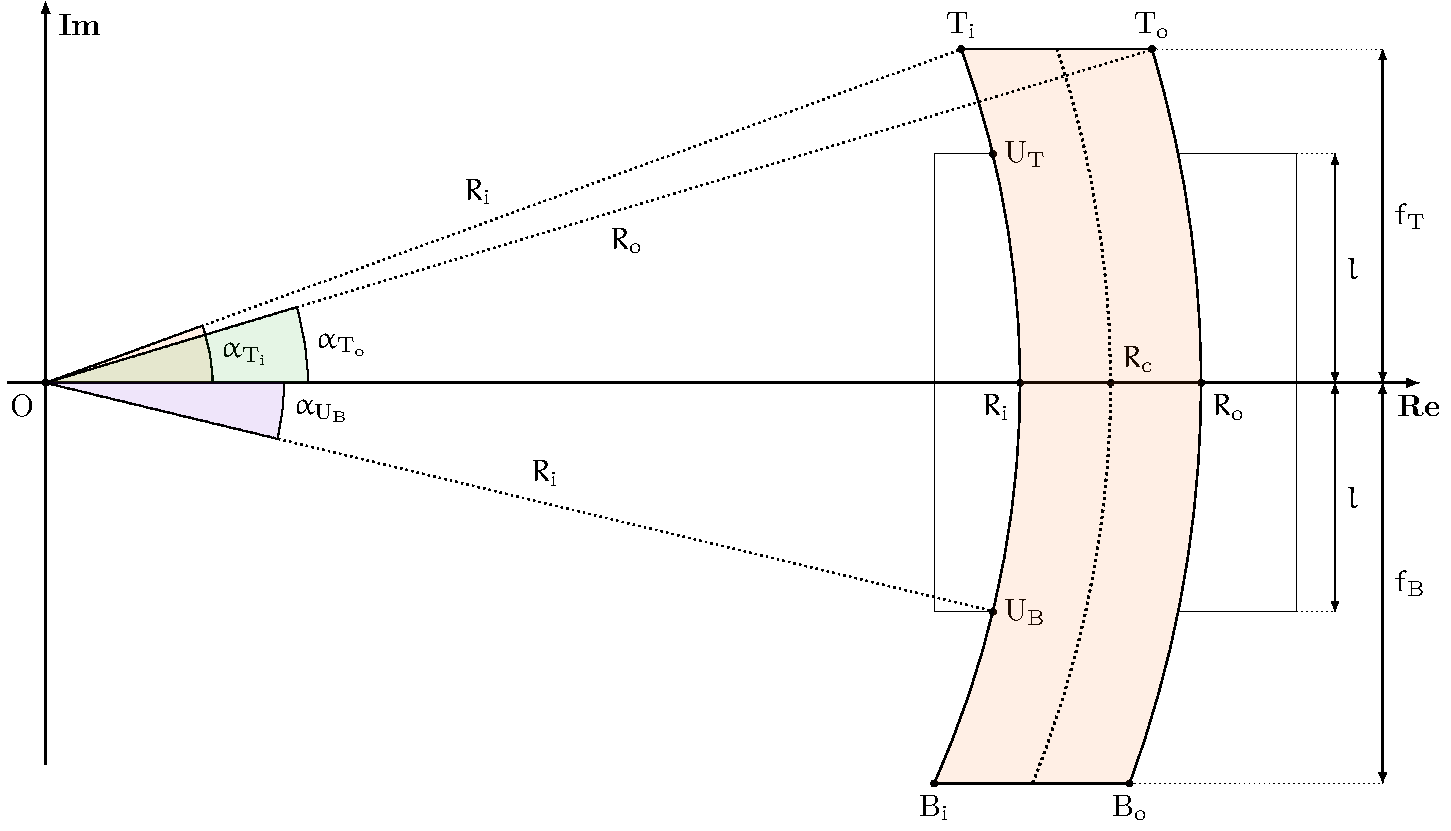
\includegraphics{RfCPN_p5_pictures/mouldoverall.pdf}
\end{adjustbox}
\end{Figlandscape}%
\end{figure}
%%%%%%%%%%%%%%%%%%%%%%%%%%%%%%%%%%%%%%%%%%%%%%%%%%%%%%%%%%
%%%%%%%%%%%%%%%%%%%%%%%%%%%%%%%%%%%%%%%%%%%%%%%%%%%%%%%%%%
%%%%%%%%%%%%%%%%%%%%%%%%%%%%%%%%%%%%%%%%%%%%%%%%%%%%%%%%%%


%%%%%%%%%%%%%%%%%%%%%%%%%%%%%%%%%%%%%%%%%%%%%%%%%%%%%%%%%%
%% subsection 1.1.1 %%%%%%%%%%%%%%%%%%%%%%%%%%%%%%%%%%%%%%
%%%%%%%%%%%%%%%%%%%%%%%%%%%%%%%%%%%%%%%%%%%%%%%%%%%%%%%%%%
\subsection{スペーサを用いた再振分け}
\index{モールド}モールドの\index{わんきょく(モールド)@湾曲(モールド)}湾曲における円の中心\index{O(わんきょくちゅうしん)@O(湾曲中心)}Oを\index{げんてんO@原点O}原点とした\index{ふくそへいめん@複素平面}複素平面を考える
%% footnote %%%%%%%%%%%%%%%%%%%%%
\footnote{ここでは$0 < R_\mathrm c < \infty$ ($0 < \nicefrac1{R_\mathrm c} < \infty$)としている。
$R_\mathrm c \to \infty$ ($\nicefrac1{R_\mathrm c} \to 0$)の場合、すなわち\index{わんきょくのないモールド@湾曲のないモールド}湾曲のないまっすぐなモールドの場合は、別途考える必要がある。}。
%%%%%%%%%%%%%%%%%%%%%%%%%%%%%%%%%
このとき、\pageautoref{fig:mouldOnComplexPlane1}のように、$R_\mathrm c$, $R_\mathrm i$, $R_\mathrm o$, $f_\mathrm T$, $f_\mathrm B$, $l$, $\alpha_{\mathrm T_\mathrm i}$, $\alpha_{\mathrm T_\mathrm o}$, $\alpha_{\mathrm U_\mathrm B}$をとると、
\begin{subequations}
%% label{eq:constraintUpoint1}
%% label{eq:constraintUpoint2}
\begin{gather}
  \label{eq:constraintUpoint1}
  R_\mathrm o - R_\mathrm c = R_\mathrm c - R_\mathrm i = \frac{W_x}2~, \qquad
  \IP\left(R_\mathrm oe^{i\alpha_{\mathrm T_\mathrm o}} - R_\mathrm ie^{i\alpha_{\mathrm T_\mathrm i}}\right)
  = 0~,\\
  \label{eq:constraintUpoint2}
  \sin\alpha_{\mathrm T_\mathrm i} = \frac{f_\mathrm T}{R_\mathrm i}, \qquad
  \sin\alpha_{\mathrm U_\mathrm B} = \frac l{R_\mathrm i}, \qquad
  \tan\theta = \frac{\delta_\mathrm s}{2l}~.
\end{gather}
\end{subequations}
ここで$W_x$はモールドの(AC)外径、$\delta_\mathrm s$は\index{スペーサあつ@スペーサ厚}スペーサの厚さ(\textbf{スペーサ厚})である。
このときモールドを原点Oを中心に$\Omega$だけ回転し、さらに点U$_\mathrm B$($R_\mathrm i$, $-\alpha_{\mathrm U_\mathrm B}$)を中心に$-\theta$だけ回転すると、点T$_\mathrm i$($R_\mathrm i$, $\alpha_{\mathrm T_\mathrm i}$)は、
%% label{eq:afterftUpoint}
\begin{align}
  \notag
  & e^{-i\theta}\left\{R_\mathrm ie^{i(\alpha_{\mathrm T_\mathrm i} + \Omega)} - R_\mathrm ie^{-i\alpha_{\mathrm U_\mathrm B}}\right\}
    +R_\mathrm ie^{-i\alpha_{\mathrm U_\mathrm B}}\\
  &= R_\mathrm i
     \left\{
       e^{i(\alpha_{\mathrm T_\mathrm i} + \Omega - \theta)} - e^{-i(\alpha_{\mathrm U_\mathrm B} + \theta)} + e^{-i\alpha_{\mathrm U_\mathrm B}}
     \right\}
  \label{eq:afterftUpoint}
\end{align}
に移動する。
また同様に点T$_\mathrm o$($R_\mathrm o$, $\alpha_{\mathrm T_\mathrm o}$)は
\begin{align*}
  \notag
  R_\mathrm oe^{i(\alpha_{\mathrm T_\mathrm o} + \Omega - \theta)}
  -R_\mathrm i\left\{e^{-i(\alpha_{\mathrm U_\mathrm B} + \theta)}-e^{-i\alpha_{\mathrm U_\mathrm B}}\right\}
\end{align*}
に移動する。
したがって、これらの差
\begin{align*}
  \notag
  e^{i(\Omega - \theta)}\left(R_\mathrm oe^{i\alpha_{\mathrm T_\mathrm o}} - R_\mathrm ie^{i\alpha_{\mathrm T_\mathrm i}}\right)
\end{align*}
の虚部が0であればよい。
つまり、\pageeqref{eq:constraintUpoint1}より、$\Omega = \theta$である
%% footnote %%%%%%%%%%%%%%%%%%%%%
\footnote{ここでは$0 \leq \Omega, \theta < \nicefrac \pi2$としている。}。
%%%%%%%%%%%%%%%%%%%%%%%%%%%%%%%%%

スペーサを入れた後の(トップ側の)振分長は、\pageeqref{eq:afterftUpoint}の虚部を見ればよい。
\begin{align*}
  R_\mathrm i\left\{\sin\alpha_{\mathrm T_\mathrm i} + \sin(\alpha_{\mathrm U_\mathrm B} + \theta) - \sin\alpha_{\mathrm U_\mathrm B}\right\}
  &= f_\mathrm T -l
     +R_\mathrm i\left(\sin\alpha_{\mathrm U_\mathrm B}\cos\theta + \cos\alpha_{\mathrm U_\mathrm B}\sin\theta\right)\\
  &= f_\mathrm T -l+l\cdot\frac{2l}{\sqrt{4l^2+\delta_\mathrm s^2}}
     +\sqrt{R_\mathrm i^2-l^2}\cdot\frac{\delta_\mathrm s}{\sqrt{4l^2+\delta_\mathrm s^2}}\\
  &= f_\mathrm T -l+\frac{2l^2+\delta_\mathrm s\sqrt{R_\mathrm i^2-l^2}}{\sqrt{4l^2+\delta_\mathrm s^2}}~.
\end{align*}
まとめると、厚さ$\delta_\mathrm s$の\index{スペーサ}スペーサを入れた後のトップ側の\index{ふりわけちょう@振分長}振分長$f'_\mathrm T$は、
\begin{align*}
  f'_\mathrm T
  = f_\mathrm T -l
    +\frac{2l^2+\delta_\mathrm s\sqrt{\left(R_\mathrm c-\nicefrac{W_x}2\right)^2-l^2}}{\sqrt{4l^2+\delta_\mathrm s^2}}~.
\end{align*}


%%%%%%%%%%%%%%%%%%%%%%%%%%%%%%%%%%%%%%%%%%%%%%%%%%%%%%%%%%
%% subsection 1.1.2 %%%%%%%%%%%%%%%%%%%%%%%%%%%%%%%%%%%%%%
%%%%%%%%%%%%%%%%%%%%%%%%%%%%%%%%%%%%%%%%%%%%%%%%%%%%%%%%%%
\subsection{振分長が均等になるスペーサ厚}
%%%%%%%%%%%%%%%%%%%%%%%%%%%%%%%
トップ側とボトム側の\index{きんとうふりわけ@均等振分}振分長が同じになるとき、$\delta_\mathrm s$は
\begin{align*}
  f'_\mathrm T - f_\mathrm T = \frac{f_\mathrm B - f_\mathrm T}2
\end{align*}
を満たす。
これより、
\begin{align*}
  \frac{2l^2+\delta_\mathrm s\sqrt{R_\mathrm i^2-l^2}}{\sqrt{4l^2+\delta_\mathrm s^2}} = l'\qquad
  \left(l' \equiv l + \frac{f_\mathrm B-f_\mathrm T}2\right)
\end{align*}
両辺を2乗すると、
\begin{gather*}
  4l^4+\delta_\mathrm s^2\left(R_\mathrm i^2-l^2\right)+4l^2\delta_\mathrm s\sqrt{R_\mathrm i^2-l^2}
  = l'^2\left(4l^2+\delta_\mathrm s^2\right)\\
  \longrightarrow\quad
  \delta_\mathrm s^2\left(R_\mathrm i^2-l^2-l'^2\right)
  +4l^2\delta_\mathrm s\sqrt{R_\mathrm i^2-l^2} -4l^2\left(l'^2 - l^2\right)
  = 0.
\end{gather*}
$\delta_\mathrm s > 0$より、
\begin{align*}
  \delta_\mathrm s
  &= \frac{\sqrt{4l^4\left(R_\mathrm i^2-l^2\right)
                 +4l^2\left(R_\mathrm i^2-l^2-l'^2\right)\left(l'^2 - l^2\right)}
           -2l^2\sqrt{R_\mathrm i^2-l^2}}{R_\mathrm i^2-l^2-l'^2}\\
  &= 2l\cdot\frac{l'\sqrt{R_\mathrm i^2-l'^2}-l\sqrt{R_\mathrm i^2-l^2}}{R_\mathrm i^2-l^2-l'^2}
\end{align*}
まとめると、求める\index{スペーサあつ@スペーサ厚}スペーサ厚$\delta_\mathrm s$は、
\begin{align*}
  \delta_\mathrm s
  = 2l\cdot
    \frac{\displaystyle
          \left(l+\frac{f_\mathrm B-f_\mathrm T}2\right)
          \sqrt{\left(R_\mathrm c-\frac{W_x}2\right)^2
                -\left(l+\frac{f_\mathrm B-f_\mathrm T}2\right)^2}
          -l\sqrt{\left(R_\mathrm c-\frac{W_x}2\right)^2-l^2}}
         {\displaystyle
          \left(R_\mathrm c-\frac{W_x}2\right)^2-l^2
          -\left(l+\frac{f_\mathrm B-f_\mathrm T}2\right)^2}~.
\end{align*}



\clearpage
%%%%%%%%%%%%%%%%%%%%%%%%%%%%%%%%%%%%%%%%%%%%%%%%%%%%%%%%%%
%% section 20.2 %%%%%%%%%%%%%%%%%%%%%%%%%%%%%%%%%%%%%%%%%%
%%%%%%%%%%%%%%%%%%%%%%%%%%%%%%%%%%%%%%%%%%%%%%%%%%%%%%%%%%
\modHeadsection{受板がある場合}
\index{ジグ}ジグの\index{ワーク}ワークと接する部品(\index{うけいた@受板}\textbf{受板})の大きさを考慮した場合を考える。
ワークに接する側の面は半径$\rho$の円弧(\index{うけいたのけい@受板の径}受板の径), 虚軸方向の厚み(\index{うけいたのはば@受板の幅}受板の幅)は$\sigma$とする。
また受板の虚軸負方向側の面は、ジグのそれと同じ平面上にあるものとする。
%%%%%%%%%%%%%%%%%%%%%%%%%%%%%%%%%%%%%%%%%%%%%%%%%%%%%%%%%%
%% figure %%%%%%%%%%%%%%%%%%%%%%%%%%%%%%%%%%%%%%%%%%%%%%%%
%%%%%%%%%%%%%%%%%%%%%%%%%%%%%%%%%%%%%%%%%%%%%%%%%%%%%%%%%%
\begin{figure}[p]%
\begin{Figbox}[valign=top]%
\resizebox{\linewidth-35pt}{!}{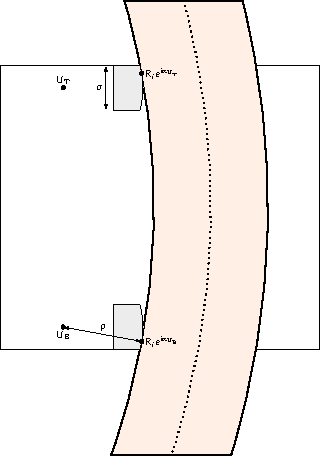
\includegraphics{RfCPN_p5_pictures/mouldUkeita.pdf}}%
\vfill~
\captionof{figure}[受板がある場合]{%
 \index{うけいた@受板}受板がある場合\newline
 $\rho$, $\sigma$は\index{うけいたのけい@受板の径}受板の径および\index{うけいたのはば@受板の幅}受板の幅を示し、U$_\mathrm T$, U$_\mathrm B$はそれぞれの受板の円弧の中心点を示す。
 受板があると\index{ワーク}ワークとの\index{せってん(ワークとうけいた)@接点(ワークと受板)}接点U$_\mathrm B$の位置も変化する。
 なお受板は、トップ側とボトム側で同じものであり、その片面はジグの片面と揃える形で装着されるものとする。
 }%\label{fig:mouldwithukeita}
\end{Figbox}%
\end{figure}%
%%%%%%%%%%%%%%%%%%%%%%%%%%%%%%%%%%%%%%%%%%%%%%%%%%%%%%%%%%
%%%%%%%%%%%%%%%%%%%%%%%%%%%%%%%%%%%%%%%%%%%%%%%%%%%%%%%%%%
%%%%%%%%%%%%%%%%%%%%%%%%%%%%%%%%%%%%%%%%%%%%%%%%%%%%%%%%%%
\index{うけいたのちゅうしん@受板の中心}受板の径の中心を改めてU$_\mathrm B$とし、また\index{げんてんO@原点O}原点Oに対する\index{へんかく(うけいた)@偏角(受板)}偏角を改めて$-\alpha_{\mathrm U_\mathrm B}$とすると、これはU$_\mathrm B$($R_\mathrm i-\rho$, $-\alpha_{\mathrm U_\mathrm B}$)と表すことができる。
ただし、\pageeqref{eq:constraintUpoint2}は以下のようになる。
\begin{align*}
  \sin\alpha_{\mathrm U_\mathrm B} = \frac{\bar l}{R_\mathrm i-\rho}\quad, \quad
  \tan\psi = \frac{\delta_\mathrm s}{2\bar l} \quad
  \left(~\bar l \equiv l-\frac\sigma2~\right).
\end{align*}
これを原点Oを中心に$\Omega$だけ回転し、さらに点U$_\mathrm B$($R_\mathrm i-\rho$, $-\alpha_{\mathrm U_\mathrm B}$)を中心に点T$_\mathrm i$($R_\mathrm i$, $\alpha_{\mathrm T_\mathrm i}$)を$-\theta$だけ回転すると、
%% label{eq:afterftUfinite}
\begin{align}
  \notag
  & e^{-i\theta}\!
    \left\{R_\mathrm ie^{i(\alpha_{\mathrm T_\mathrm i}+\Omega)}
           -R_\mathrm i'e^{-i\alpha_{\mathrm U_\mathrm B}}\right\}
    +R_\mathrm i'e^{-i\alpha_{\mathrm U_\mathrm B}}\\
  & = R_\mathrm ie^{i(\alpha_{\mathrm T_\mathrm i}+\Omega-\theta)}
      -R_\mathrm i'\!
       \left\{e^{-i(\alpha_{\mathrm U_\mathrm B}+\theta)}-e^{-i\alpha_{\mathrm U_\mathrm B}}\right\}\qquad
    \big(R_\mathrm i' \equiv R_\mathrm i-\rho\big)
    \label{eq:afterftUfinite}
\end{align}
に移動する。
同様に点T$_\mathrm o$($R_\mathrm o$, $\alpha_{\mathrm T_\mathrm o}$)は
\begin{align*}
  R_\mathrm oe^{i(\alpha_{\mathrm T_\mathrm o}+\Omega-\theta)}
  -R_\mathrm i'\!
   \left\{e^{-i(\alpha_{\mathrm U_\mathrm B} + \theta)} - e^{-i\alpha_{\mathrm U_\mathrm B}}\right\}
\end{align*}
に移動する。
したがって、これらの差
\begin{align*}
  e^{i(\Omega-\theta)}
  \left(R_\mathrm oe^{i\alpha_{\mathrm T_\mathrm o}} - R_\mathrm ie^{i\alpha_{\mathrm T_\mathrm i}}\right)
\end{align*}
の虚部が0であればよい。
つまり、\pageeqref{eq:constraintUpoint1}より、受板がある場合も$\Omega = \theta$である。


%%%%%%%%%%%%%%%%%%%%%%%%%%%%%%%%%%%%%%%%%%%%%%%%%%%%%%%%%%
%% subsection 20.2.1 %%%%%%%%%%%%%%%%%%%%%%%%%%%%%%%%%%%%%
%%%%%%%%%%%%%%%%%%%%%%%%%%%%%%%%%%%%%%%%%%%%%%%%%%%%%%%%%%
\subsection{受板の接点}
\index{うけいた@受板}受板とワークとの(トップ側の)接点は、$R_\mathrm ie^{i\alpha_{\mathrm U_\mathrm B}}$で与えられる。
このとき厚さ$\delta_\mathrm s$のスペーサを取付けると、U$_\mathrm B$を中心に回転するが、それに伴い\index{ワークとジグのせってん@ワークとジグの接点}受板との接点の位置も変化する。

%%%%%%%%%%%%%%%%%%%%%%%%%%%%%%%%%%%%%%%%%%%%%%%%%%%%%%%%%%
%% subsubsection 19.2.1.1 %%%%%%%%%%%%%%%%%%%%%%%%%%%%%%%%
%%%%%%%%%%%%%%%%%%%%%%%%%%%%%%%%%%%%%%%%%%%%%%%%%%%%%%%%%%
\subsubsection{回転後のモールドの湾曲中心}
%%%%%%%%%%%%%%%%%%%%%%%%%
厚さ$\delta_\mathrm s$の\index{スペーサ}スペーサを挟むと、トップ側における\index{うけいたのちゅうしん@受板の中心}受板の円の中心U$_\mathrm B$は実軸方向に$\delta_\mathrm s$だけ移動するので、
\begin{align*}
  R_\mathrm i'e^{i\alpha_{\mathrm U_\mathrm B}}
  \quad\longrightarrow\quad
  \delta_\mathrm s+R_\mathrm i'e^{i\alpha_{\mathrm U_\mathrm B}}\ .
\end{align*}
よって、それぞれの受板の中心U$_\mathrm B$, U$_\mathrm T$を結んだ線分U$_\mathrm B$U$_\mathrm T$は、U$_\mathrm B$を中心に$-\psi$だけ傾いた線分U$_\mathrm B'$U$_\mathrm T'$となる
%% footnote %%%%%%%%%%%%%%%%%%%%%
\footnote{%
U$_\mathrm B'$U$_\mathrm T'$の長さは$\bar l\sec\psi$であり、U$_\mathrm B$U$_\mathrm T$の長さ$\bar l$より長くなることに注意。}。
%%%%%%%%%%%%%%%%%%%%%%%%%%%%%%%%%
\index{かいてんごのわんきょくちゅうしん@回転後の湾曲中心}回転後のワークの湾曲中心は、この線分の垂直二等分線上にあり、またそれぞれの受板の中心から$R_\mathrm i'$の距離の位置にある。
つまり、この傾いた線分U$_\mathrm B'$U$_\mathrm T'$の中点から、角度$\pi-\psi$, 大きさ$\sqrt{R_\mathrm i'^2-\frac{\delta_\mathrm s^2+(2\bar l)^2}4}$の位置に移動する。
したがって、回転後における湾曲中心O$'$は、
%% label{eq:afterOrgin}
\begin{align}
  \notag
  & \frac{\delta_\mathrm s}2+\sqrt{R_\mathrm i'^2-\bar l^2}
    +\sqrt{R_\mathrm i'^2-\frac{\delta_\mathrm s^2+(2\bar l)^2}4}e^{i(\pi-\psi)}\\
  & = \frac{\delta_\mathrm s}2+\sqrt{R_\mathrm i'^2-\bar l^2}-\sqrt{R_\mathrm i'^2-\frac{\delta_\mathrm s^2+(2\bar l)^2}4}\cos\psi
      +i\sqrt{R_\mathrm i'^2-\frac{\delta_\mathrm s^2+(2\bar l)^2}4}\sin\psi\ .
    \label{eq:afterOrgin}
\end{align}

\clearpage
%%%%%%%%%%%%%%%%%%%%%%%%%%%%%%%%%%%%%%%%%%%%%%%%%%%%%%%%%%
%% subsubsection 19.2.1.2 %%%%%%%%%%%%%%%%%%%%%%%%%%%%%%%%
%%%%%%%%%%%%%%%%%%%%%%%%%%%%%%%%%%%%%%%%%%%%%%%%%%%%%%%%%%
\subsubsection{回転後の接点(トップ側)}
\index{かいてんごのうけいたのちゅうしん@回転後の受板の中心}回転後のトップ側における受板の中心U$_\mathrm T'$と\index{かいてんごのわんきょくちゅうしん@回転後の湾曲中心}湾曲中心O$'$との差をとると、
\begin{align*}
  \frac{\delta_\mathrm s}2+\sqrt{R_\mathrm i'^2-\frac{\delta_\mathrm s^2+(2\bar l)^2}4}\cos\psi
  +i\left\{\bar l-\sqrt{R_\mathrm i'^2-\frac{\delta_\mathrm s^2+(2\bar l)^2}4}\sin\psi\right\}
  = R_\mathrm i'e^{i\alpha'_{\mathrm U_\mathrm T}}\ .
\end{align*}
ここで、
\begin{align*}
  \tan\alpha'_{\mathrm U_\mathrm T}
  = \frac{\displaystyle\bar l-\sqrt{R_\mathrm i'^2-\frac{\delta_\mathrm s^2+(2\bar l)^2}4}\sin\psi}
         {\displaystyle\frac{\delta_\mathrm s}2+\sqrt{R_\mathrm i'^2-\frac{\delta_\mathrm s^2+(2\bar l)^2}4}\cos\psi}\ .
\end{align*}
%%%%%%%%%%%%%%%%%%%%%%%%%%%%%%%%%%%%%%%%%%%%%%%%%%%%%%%%%%
%% hosoku %%%%%%%%%%%%%%%%%%%%%%%%%%%%%%%%%%%%%%%%%%%%%%%%
%%%%%%%%%%%%%%%%%%%%%%%%%%%%%%%%%%%%%%%%%%%%%%%%%%%%%%%%%%
\begin{hosoku}
これの大きさは、$\delta_\mathrm s\cos\psi-2\bar l\sin\psi = 0$より、
\begin{align*}
  \left\{\frac{\delta_\mathrm s}2+\sqrt{R_\mathrm i'^2-\frac{\delta_\mathrm s^2+(2\bar l)^2}4}\cos\psi\right\}^2
  +\left\{\bar l-\sqrt{R_\mathrm i'^2-\frac{\delta_\mathrm s^2+(2\bar l)^2}4}\sin\psi\right\}^2
  = R_\mathrm i'^2\ .
\end{align*}
\end{hosoku}
%%%%%%%%%%%%%%%%%%%%%%%%%%%%%%%%%%%%%%%%%%%%%%%%%%%%%%%%%%
%%%%%%%%%%%%%%%%%%%%%%%%%%%%%%%%%%%%%%%%%%%%%%%%%%%%%%%%%%
%%%%%%%%%%%%%%%%%%%%%%%%%%%%%%%%%%%%%%%%%%%%%%%%%%%%%%%%%%
よって、回転後の接点は以下で与えられる。
\begin{align*}
  &  R_\mathrm ie^{i\alpha'_{\mathrm U_\mathrm T}}
     +\frac{\delta_\mathrm s}2+\sqrt{R_\mathrm i'^2-\bar l^2}-\sqrt{R_\mathrm i'^2-\frac{\delta_\mathrm s^2+(2\bar l)^2}4}\cos\psi
     +i\sqrt{R_\mathrm i'^2-\frac{\delta_\mathrm s^2+(2\bar l)^2}4}\sin\psi\\
  &= \delta_\mathrm s+R_\mathrm i'e^{i\alpha_{\mathrm U_\mathrm B}}+\rho e^{i\alpha'_{\mathrm U_\mathrm T}}\ .
\end{align*}

%%%%%%%%%%%%%%%%%%%%%%%%%%%%%%%%%%%%%%%%%%%%%%%%%%%%%%%%%%
%% subsubsection 1.2.1.3 %%%%%%%%%%%%%%%%%%%%%%%%%%%%%%%%%
%%%%%%%%%%%%%%%%%%%%%%%%%%%%%%%%%%%%%%%%%%%%%%%%%%%%%%%%%%
\subsubsection{回転後の接点(ボトム側)}
回転後のボトム側における受板の中心U$_\mathrm B$と\index{わんきょくちゅうしん@湾曲中心}湾曲中心O$'$との差をとると、
\begin{align*}
  -\frac{\delta_\mathrm s}2+\sqrt{R_\mathrm i'^2-\frac{\delta_\mathrm s^2+(2\bar l)^2}4}\cos\psi
  -i\left\{\bar l+\sqrt{R_\mathrm i'^2-\frac{\delta_\mathrm s^2+(2\bar l)^2}4}\sin\psi\right\}
  = R_\mathrm i'e^{-i\alpha'_{\mathrm U_\mathrm B}}
\end{align*}
ここで、
\begin{align*}
  \tan\alpha'_{\mathrm U_\mathrm B}
  = \frac{\displaystyle\bar l+\sqrt{R_\mathrm i'^2-\frac{\delta_\mathrm s^2+(2\bar l)^2}4}\sin\psi}
         {\displaystyle-\frac{\delta_\mathrm s}2+\sqrt{R_\mathrm i'^2-\frac{\delta_\mathrm s^2+(2\bar l)^2}4}\cos\psi}
\end{align*}
よって、回転後の接点は以下で与えられる。
%% label{eq:afterUBcontact}
\begin{align}
  \notag
  &  R_\mathrm ie^{-i\alpha'_{\mathrm U_\mathrm B}}
     +\frac{\delta_\mathrm s}2+\sqrt{R_\mathrm i'^2-\bar l^2}-\sqrt{R_\mathrm i'^2-\frac{\delta_\mathrm s^2+(2\bar l)^2}4}\cos\psi
     +i\sqrt{R_\mathrm i'^2-\frac{\delta_\mathrm s^2+(2\bar l)^2}4}\sin\psi\\
  &= R_\mathrm i'e^{-i\alpha_{\mathrm U_\mathrm B}}+\rho e^{-i\alpha'_{\mathrm U_\mathrm B}}
   \label{eq:afterUBcontact}
\end{align}
%%%%%%%%%%%%%%%%%%%%%%%%%%%%%%%%%%%%%%%%%%%%%%%%%%%%%%%%%%
%% hosoku %%%%%%%%%%%%%%%%%%%%%%%%%%%%%%%%%%%%%%%%%%%%%%%%
%%%%%%%%%%%%%%%%%%%%%%%%%%%%%%%%%%%%%%%%%%%%%%%%%%%%%%%%%%
\begin{hosoku}
辺の長さが$R_i'$, $R_i'$, $2\bar l$の二等辺三角形$\triangle$OU$_\mathrm B$U$_\mathrm T$の部分が、回転後には辺の長さ$R_i'$, $R_i'$, $\sqrt{\delta_\mathrm s^2+(2\bar l)^2}$の二等辺三角形$\triangle$O$'$U$_\mathrm B'$U$_\mathrm T'$となる。
実際、$\cos2a = 1-2\sin^2\!a$より、
\begin{align*}
  \sin^2\frac{\alpha'_{\mathrm U_\mathrm T}+\alpha'_{\mathrm U_\mathrm B}}2
  = \frac{\delta_\mathrm s^2+(2\bar l)^2}{4R_\mathrm i'^2}\ .
\end{align*}
\end{hosoku}
%%%%%%%%%%%%%%%%%%%%%%%%%%%%%%%%%%%%%%%%%%%%%%%%%%%%%%%%%%
%%%%%%%%%%%%%%%%%%%%%%%%%%%%%%%%%%%%%%%%%%%%%%%%%%%%%%%%%%
%%%%%%%%%%%%%%%%%%%%%%%%%%%%%%%%%%%%%%%%%%%%%%%%%%%%%%%%%%


%%%%%%%%%%%%%%%%%%%%%%%%%%%%%%%%%%%%%%%%%%%%%%%%%%%%%%%%%%
%% subsection 1.2.2 %%%%%%%%%%%%%%%%%%%%%%%%%%%%%%%%%%%%%%
%%%%%%%%%%%%%%%%%%%%%%%%%%%%%%%%%%%%%%%%%%%%%%%%%%%%%%%%%%
\subsection{スペーサによるモールドの回転角}
厚さ$\delta_\mathrm s$の\index{スペーサ}スペーサを挿入すると、\index{わんきょくちゅうしん@湾曲中心}湾曲中心Oは、U$_\mathrm B$を中心に$-\left(\alpha'_{\mathrm U_\mathrm B}\!-\alpha_{\mathrm U_\mathrm B}\right)$だけ回転する。
実際、
\begin{align*}
  -R_\mathrm i'e^{-i\alpha'_{\mathrm U_\mathrm B}}+R_\mathrm i'e^{-i\alpha_{\mathrm U_\mathrm B}}
  &= R_\mathrm i'(\cos\alpha_{\mathrm U_\mathrm B}-\cos\alpha'_{\mathrm U_\mathrm B})
     +iR_\mathrm i'(\sin\alpha'_{\mathrm U_\mathrm B}-\sin\alpha_{\mathrm U_\mathrm B})
\end{align*}
であり、これは\index{かいてんごのわんきょくちゅうしん@回転後の湾曲中心}回転後の湾曲中心\pageeqref{eq:afterOrgin}に一致する。
つまり、$\alpha'_{\mathrm U_\mathrm B}\!-\alpha_{\mathrm U_\mathrm B}$が$\theta$に相当する。
%%%%%%%%%%%%%%%%%%%%%%%%%%%%%%%%%%%%%%%%%%%%%%%%%%%%%%%%%%
%% hosoku %%%%%%%%%%%%%%%%%%%%%%%%%%%%%%%%%%%%%%%%%%%%%%%%
%%%%%%%%%%%%%%%%%%%%%%%%%%%%%%%%%%%%%%%%%%%%%%%%%%%%%%%%%%
\begin{hosoku}
トップ側の接点U$_\mathrm T'$とボトム側の接点U$_\mathrm B'$の差をとると、
\begin{align*}
  R_\mathrm i\left(e^{i\alpha_{\mathrm U_\mathrm T}'}-e^{-i\alpha'_{\mathrm U_\mathrm B}}\right)
  &= \frac{R_\mathrm i'+\rho}{R_\mathrm i'}\left\{\delta_\mathrm s+i(2\bar l)\right\}
   = \frac{R_\mathrm i}{R_\mathrm i'}\sqrt{\delta_\mathrm s^2+(2\bar l)^2}e^{i(\nicefrac\pi2-\psi)}\ .
\end{align*}
したがって、厚さ$\delta_\mathrm s$のスペーサを挿入すると、両接点を通る直線は$-\psi$だけ傾くことがわかる。
また、その長さは受板中心間U$_\mathrm T'$U$_\mathrm B'$の距離$\sqrt{\delta_\mathrm s^2+(2\bar l)^2}$の$\nicefrac{R_i}{R_i'}$倍になっていることも確かめられる。
\end{hosoku}
%%%%%%%%%%%%%%%%%%%%%%%%%%%%%%%%%%%%%%%%%%%%%%%%%%%%%%%%%%
%%%%%%%%%%%%%%%%%%%%%%%%%%%%%%%%%%%%%%%%%%%%%%%%%%%%%%%%%%
%%%%%%%%%%%%%%%%%%%%%%%%%%%%%%%%%%%%%%%%%%%%%%%%%%%%%%%%%%


%%%%%%%%%%%%%%%%%%%%%%%%%%%%%%%%%%%%%%%%%%%%%%%%%%%%%%%%%%
%% subsection 1.2.3 %%%%%%%%%%%%%%%%%%%%%%%%%%%%%%%%%%%%%%
%%%%%%%%%%%%%%%%%%%%%%%%%%%%%%%%%%%%%%%%%%%%%%%%%%%%%%%%%%
\subsection{スペーサによる再振分け}

%%%%%%%%%%%%%%%%%%%%%%%%%%%%%%%%%%%%%%%%%%%%%%%%%%%%%%%%%%
%% subsubsection 1.2.3.1 %%%%%%%%%%%%%%%%%%%%%%%%%%%%%%%%%
%%%%%%%%%%%%%%%%%%%%%%%%%%%%%%%%%%%%%%%%%%%%%%%%%%%%%%%%%%
\subsubsection{再振分長}
\index{スペーサ}スペーサを入れた後のトップ側の\index{ふりわけちょう@振分長}振分長(\index{さいふりわけちょう@再振分長}\textbf{再振分長})$f'_\mathrm T$は、\pageeqref{eq:afterftUfinite}の虚部を見ればよい。
回転角は$-(\alpha'_{\mathrm U_\mathrm B}-\alpha_{\mathrm U_\mathrm B})$なので、
\begin{align*}
  f'_\mathrm T
  = R_\mathrm i\sin\alpha_{\mathrm T_\mathrm i}
    +R_\mathrm i'\left(\sin\alpha'_{\mathrm U_\mathrm B}-\sin\alpha_{\mathrm U_\mathrm B}\right)
  &= f_\mathrm T+\sqrt{R_\mathrm i'^2-\frac{\delta_\mathrm s^2+(2\bar l)^2}4}\sin\psi\\
  &= f_\mathrm T+\sqrt{R_\mathrm i'^2-\frac{\delta_\mathrm s^2+(2\bar l)^2}4}\frac{\delta_\mathrm s}{\sqrt{\delta_\mathrm s^2+(2\bar l)^2}}\ .
\end{align*}

%%%%%%%%%%%%%%%%%%%%%%%%%%%%%%%%%%%%%%%%%%%%%%%%%%%%%%%%%%
%% subsubsection 1.2.3.2 %%%%%%%%%%%%%%%%%%%%%%%%%%%%%%%%%
%%%%%%%%%%%%%%%%%%%%%%%%%%%%%%%%%%%%%%%%%%%%%%%%%%%%%%%%%%
\subsubsection{モールドの移動距離}
\pageeqref{eq:afterftUfinite}の実部は、
\begin{align*}
  & R_\mathrm i\cos\alpha_{\mathrm T_\mathrm i}
    -R_\mathrm i'(\cos\alpha'_{\mathrm U_\mathrm B}-\cos\alpha_{\mathrm U_\mathrm B})\\
  & = \sqrt{R_\mathrm i^2-f_\mathrm T^2}+\frac{\delta_\mathrm s}2+\sqrt{R_\mathrm i'^2-\bar l^2}
      -\sqrt{R_\mathrm i'^2-\frac{\delta_\mathrm s^2+(2\bar l)^2}4}\cos\psi
\end{align*}
となる。
よって、\index{スペーサ}スペーサを挿入することにより、ワークは水平・鉛直方向にそれぞれ、
\begin{subequations}
%% label{eq:spacerMoveHdistance}
\begin{alignat}{2}
  \label{eq:spacerMoveHdistance}
  \text{水平方向:}\quad
  & \frac{\delta_\mathrm s}2+\sqrt{R_\mathrm i'^2-\bar l^2}-\sqrt{R_\mathrm i'^2-\frac{\delta_\mathrm s^2+(2\bar l)^2}4}\frac{2\bar l}{\sqrt{\delta_\mathrm s^2+(2\bar l)^2}}\\
  \text{鉛直方向:}\quad
  & \sqrt{R_\mathrm i'^2-\frac{\delta_\mathrm s^2+(2\bar l)^2}4}\frac{\delta_\mathrm s}{\sqrt{\delta_\mathrm s^2+(2\bar l)^2}}
\end{alignat}
\end{subequations}
だけ移動することがわかる。


%\clearpage
%%%%%%%%%%%%%%%%%%%%%%%%%%%%%%%%%%%%%%%%%%%%%%%%%%%%%%%%%%
%% subsection 1.2.4 %%%%%%%%%%%%%%%%%%%%%%%%%%%%%%%%%%%%%%
%%%%%%%%%%%%%%%%%%%%%%%%%%%%%%%%%%%%%%%%%%%%%%%%%%%%%%%%%%
\subsection{再振分長が均等になるスペーサ厚}
トップ側とボトム側の\index{きんとうふりわけ@均等振分}振分長が同じになるとき、$\delta_\mathrm s$は
\begin{align*}
  \sqrt{R_\mathrm i'^2-\frac{\delta_\mathrm s^2+(2\bar l)^2}4}\frac{\delta_\mathrm s}{\sqrt{\delta_\mathrm s^2+(2\bar l)^2}} = f_d \qquad
  \left(f_d \equiv \frac{f_\mathrm B-f_\mathrm T}2\right)\ .
\end{align*}
を満たす。
両辺を2乗して$-4$倍すると、
\begin{align*}
  \delta_\mathrm s^2\left\{\delta_\mathrm s^2+(2\bar l)^2-4R_\mathrm i'^2\right\}+4f_d^2\left\{\delta_\mathrm s^2+(2\bar l)^2\right\}
  & = \delta_\mathrm s^4-2\left\{2R_\mathrm i'^2-2\bar l^2-2f_d^2\right\}\delta_\mathrm s^2+4f_d^2(2\bar l)^2\\
  & = 0\ .
\end{align*}
したがって、$f_\mathrm T = f_\mathrm B$ ($f_d = 0$)のとき$\delta_\mathrm s = 0$であることを考慮して、
\begin{align*}
  \delta_\mathrm s^2
  &= 2\left\{
       R_\mathrm i'^2-\bar l^2-f_d^2-\sqrt{\left(R_\mathrm i'^2-\bar l^2-f_d^2\right)^2-4f_d^2\bar l^2}\,
     \right\}\\
  &= \left(\sqrt{R_\mathrm i'^2-(\bar l-f_d)^2}-\sqrt{R_\mathrm i'^2-(\bar l+f_d)^2}\,\right)^2.
\end{align*}
なお、これはワークが水平・鉛直方向にそれぞれ、
\begin{align*}
  \text{水平方向:}~\frac{\delta_\mathrm s}2+\sqrt{R_\mathrm i^2-\bar l^2}-\frac{2\bar l}{\delta_\mathrm s}f_d\quad(\delta_\mathrm s>0)\ , \qquad
  \text{鉛直方向:}~\frac{f_\mathrm B-f_\mathrm T}2
\end{align*}
だけ移動することを意味する。
%%%%%%%%%%%%%%%%%%%%%%%%%%%%%%%%%%%%%%%%%%%%%%%%%%%%%%%%%%
%% hosoku %%%%%%%%%%%%%%%%%%%%%%%%%%%%%%%%%%%%%%%%%%%%%%%%
%%%%%%%%%%%%%%%%%%%%%%%%%%%%%%%%%%%%%%%%%%%%%%%%%%%%%%%%%%
\begin{hosoku}
改めてまとめると、厚さ$\delta_\mathrm s$のスペーサを(トップ側に)挿入した後の\index{トップふりわけちょう@トップ振分長}トップ側の振分長$f_\mathrm T'$は、
\begin{align*}
  f_\mathrm T'
  = f_\mathrm T+\sqrt{R_\mathrm i'^2-\frac{\delta_\mathrm s^2+(2\bar l)^2}4}\frac{\delta_\mathrm s}{\sqrt{\delta_\mathrm s^2+(2\bar l)^2}}\ .
\end{align*}
トップ側とボトム側の\index{きんとうふりわけ@均等振分}振分長が均等になるときの\index{スペーサあつ@スペーサ厚}スペーサ厚$\delta_\mathrm s'$は、
\begin{align*}
  \delta_\mathrm s' = \sqrt{R_\mathrm i'^2-(\bar l-f_d)^2}-\sqrt{R_\mathrm i'^2-(\bar l+f_d)^2}\ .
\end{align*}
ここで、
\begin{align*}
  R_\mathrm i' = R_\mathrm c-\frac{W_x}2-\rho\ ,\quad
  \bar l = l-\frac\sigma2\ ,\quad
  f_d = \frac{f_\mathrm B-f_\mathrm T}2\ .
\end{align*}
\end{hosoku}
%%%%%%%%%%%%%%%%%%%%%%%%%%%%%%%%%%%%%%%%%%%%%%%%%%%%%%%%%%
%%%%%%%%%%%%%%%%%%%%%%%%%%%%%%%%%%%%%%%%%%%%%%%%%%%%%%%%%%
%%%%%%%%%%%%%%%%%%%%%%%%%%%%%%%%%%%%%%%%%%%%%%%%%%%%%%%%%%



\clearpage
%%%%%%%%%%%%%%%%%%%%%%%%%%%%%%%%%%%%%%%%%%%%%%%%%%%%%%%%%%
%% section 21.3 %%%%%%%%%%%%%%%%%%%%%%%%%%%%%%%%%%%%%%%%%%
%%%%%%%%%%%%%%%%%%%%%%%%%%%%%%%%%%%%%%%%%%%%%%%%%%%%%%%%%%
\modHeadsection{テーブルの回転による振分長の調節}
これまでトップ・ボトム振分長の差を小さくするために\index{スペーサ}スペーサを用いる手法を考えてきた。
スペーサを取付けることは、本質的にはボトム側の\index{うけいた@受板}受板の点U$_\mathrm B$を中心に回転しているということである。
このとき回転の中心はU$_\mathrm B$である必要はなく、他の点でも問題ない。
したがって、スペーサを用いて回転をしなくても、\index{テーブル}テーブルそのものを回転するという手法が考えられる。
これは回転の中心が、受板の点U$_\mathrm B$から\index{テーブルちゅうしん@テーブル中心}\textbf{テーブル中心}Pに変わることに相当する。

\index{うけいたのちゅうしん@受板の中心}受板の中心U$_\mathrm B$と、テーブル中心Pとの実軸方向の距離を$\Delta$とすると、テーブル中心Pの$X$座標$\Delta'$は次で与えられる。
%% label{eq:tableCenter}
\begin{align}
  \label{eq:tableCenter}
  \Delta'
  = \Delta+R_\mathrm i'\cos\alpha_{\mathrm U_\mathrm B} = \Delta+\sqrt{R_\mathrm i'^2-\bar l^2}\ .
\end{align}
\index{トップがわのCがわそとたんてん@トップ側のC側外端点}トップ側のC側外端点T$_\mathrm i$($R_\mathrm i$, $\alpha_{\mathrm T_\mathrm i}$)を、原点Oを中心に$\Omega$だけ回転し、さらに点P\,($\Delta'$, $0$)を中心に$-\theta$だけ回転すると、
\begin{align}
  \label{eq:afterfttable}
  e^{-i\theta}\left\{R_\mathrm i^{i(\alpha_{\mathrm T_\mathrm i}+\Omega)}-\Delta'\right\}+\Delta'
  = R_\mathrm ie^{i(\alpha_{\mathrm T_\mathrm i}+\Omega-\theta)}+\Delta'\left(1-e^{-i\theta}\right)
\end{align}
に移動する。
同様に、\index{トップがわのAがわそとたんてん@トップ側のA側外端点}トップ側のA側外端点T$_\mathrm o$($R_\mathrm o$, $\alpha_{\mathrm T_\mathrm o}$)は、
\begin{align*}
  e^{-i\theta}\!\left\{R_\mathrm o^{i(\alpha_{\mathrm T_\mathrm o}+\Omega)}-\Delta'\right\}+\Delta'
  = R_\mathrm ie^{i(\alpha_{\mathrm T_\mathrm o}+\Omega-\theta)}+\Delta'\!\left(1-e^{-i\theta}\right)
\end{align*}
に移動する。
したがって、これらの差
\begin{align*}
  e^{i(\Omega-\theta)}
  \left(R_\mathrm oe^{i\alpha_{\mathrm T_\mathrm o}}-R_\mathrm ie^{i\alpha_{\mathrm T_\mathrm i}}\right)
\end{align*}
の虚部が$0$であればよい。
よって\pageeqref{eq:constraintUpoint1}より、この場合も$\Omega = \theta$となる。


%%%%%%%%%%%%%%%%%%%%%%%%%%%%%%%%%%%%%%%%%%%%%%%%%%%%%%%%%%
%% subsection 21.3.1 %%%%%%%%%%%%%%%%%%%%%%%%%%%%%%%%%%%%%
%%%%%%%%%%%%%%%%%%%%%%%%%%%%%%%%%%%%%%%%%%%%%%%%%%%%%%%%%%
\subsection{回転後のモールドの湾曲中心および受板との接点}

%%%%%%%%%%%%%%%%%%%%%%%%%%%%%%%%%%%%%%%%%%%%%%%%%%%%%%%%%%
%% subsubsection 21.3.1.1 %%%%%%%%%%%%%%%%%%%%%%%%%%%%%%%%
%%%%%%%%%%%%%%%%%%%%%%%%%%%%%%%%%%%%%%%%%%%%%%%%%%%%%%%%%%
\subsubsection{回転後のモールドの湾曲中心}
\index{かいてんごのわんきょくちゅうしん@回転後の湾曲中心}回転後の湾曲中心O$'$は、点Pを中心に$-\theta$だけ回転するので、
\begin{align*}
  \Delta'\!\left(1-e^{-i\theta}\right) = \Delta'(1-\cos\theta)+i\Delta'\sin\theta\ .
\end{align*}

%%%%%%%%%%%%%%%%%%%%%%%%%%%%%%%%%%%%%%%%%%%%%%%%%%%%%%%%%%
%% subsubsection 21.3.1.2 %%%%%%%%%%%%%%%%%%%%%%%%%%%%%%%%
%%%%%%%%%%%%%%%%%%%%%%%%%%%%%%%%%%%%%%%%%%%%%%%%%%%%%%%%%%
\subsubsection{回転後の接点}
回転後におけるトップ側の\index{ワークとうけいたのせってん@ワークと受板の接点}受板との接点は、点Pを中心に$-\theta$だけ回転するので、
\begin{align*}
  &  e^{-i\theta}\left(R_\mathrm ie^{i\alpha_{\mathrm U_\mathrm B}}-\Delta'\right)+\Delta'\\
  &= R_\mathrm ie^{i(\alpha_{\mathrm U_\mathrm B}-\theta)}+\Delta'\!\left(1-e^{-i\theta}\right)\\
  &= R_\mathrm i\cos(\alpha_{\mathrm U_\mathrm B}-\theta)+\Delta'(1-\cos\theta)
     +i\left\{R_\mathrm i\sin(\alpha_{\mathrm U_\mathrm B}-\theta)+i\Delta'\sin\theta\right\}\ .
\end{align*}
同様に、ボトム側の受板との接点は、
\begin{align*}
  &  e^{-i\theta}\left(R_\mathrm ie^{-i\alpha_{\mathrm U_\mathrm B}}-\Delta'\right)+\Delta'\\
  &= R_\mathrm ie^{-i(\alpha_{\mathrm U_\mathrm B}+\theta)}+\Delta'\!\left(1-e^{-i\theta}\right)\\
  &= R_\mathrm i\cos(\alpha_{\mathrm U_\mathrm B}+\theta)+\Delta'(1-\cos\theta)
     -i\left\{R_\mathrm i\sin(\alpha_{\mathrm U_\mathrm B}+\theta)-i\Delta'\sin\theta\right\}\ .
\end{align*}
%%%%%%%%%%%%%%%%%%%%%%%%%%%%%%%%%%%%%%%%%%%%%%%%%%%%%%%%%%
%% hosoku %%%%%%%%%%%%%%%%%%%%%%%%%%%%%%%%%%%%%%%%%%%%%%%%
%%%%%%%%%%%%%%%%%%%%%%%%%%%%%%%%%%%%%%%%%%%%%%%%%%%%%%%%%%
\begin{hosoku}
両接点との差をとると、
\begin{align*}
  2R_\mathrm i\sin\alpha_{\mathrm U_\mathrm B}\sin\theta+2iR_\mathrm i\sin\alpha_{\mathrm U_\mathrm B}\cos\theta
  = \frac{R_\mathrm i}{R_\mathrm i'}(2\bar l)e^{i(\pi-\theta)}
\end{align*}
となり、\index{うけいたのちゅうしん@受板の中心}受板の両中心間(長さ$2\bar l$)を結んだ線分を$\nicefrac{R_\mathrm i}{R_\mathrm i'}$倍し、虚軸から$-\theta$だけ傾けたものになっていることがわかる。
\end{hosoku}
%%%%%%%%%%%%%%%%%%%%%%%%%%%%%%%%%%%%%%%%%%%%%%%%%%%%%%%%%%
%%%%%%%%%%%%%%%%%%%%%%%%%%%%%%%%%%%%%%%%%%%%%%%%%%%%%%%%%%
%%%%%%%%%%%%%%%%%%%%%%%%%%%%%%%%%%%%%%%%%%%%%%%%%%%%%%%%%%


%%%%%%%%%%%%%%%%%%%%%%%%%%%%%%%%%%%%%%%%%%%%%%%%%%%%%%%%%%
%% subsection 21.3.2 %%%%%%%%%%%%%%%%%%%%%%%%%%%%%%%%%%%%%
%%%%%%%%%%%%%%%%%%%%%%%%%%%%%%%%%%%%%%%%%%%%%%%%%%%%%%%%%%
\subsection{回転後の振分長}
回転後の\index{トップさいふりわけちょう@トップ再振分長}トップ側の振分長$f_\mathrm T'$は、\pageeqref{eq:afterfttable}の虚部を見ればよいので、
\begin{subequations}
%\label{eq:saifuriwake}
\begin{align}
  \label{eq:saifuriwakeT}
  f_\mathrm T'
  = f_\mathrm T+\Delta'\sin\theta
  = f_\mathrm T+\left(\Delta+\sqrt{R_\mathrm i'-\bar l^2}\right)\sin\theta\ .
\end{align}
同様に、\index{ボトムさいふりわけちょう@ボトム再振分長}ボトムの振分長$f_\mathrm B'$は、符号に注意して、
\begin{align}
  f_\mathrm B' = f_\mathrm B-\Delta'\sin\theta = (f_\mathrm T+f_\mathrm B)-f_\mathrm T'\ .
\end{align}
\end{subequations}
%%%%%%%%%%%%%%%%%%%%%%%%%%%%%%%%%%%%%%%%%%%%%%%%%%%%%%%%%%
%% hosoku %%%%%%%%%%%%%%%%%%%%%%%%%%%%%%%%%%%%%%%%%%%%%%%%
%%%%%%%%%%%%%%%%%%%%%%%%%%%%%%%%%%%%%%%%%%%%%%%%%%%%%%%%%%
\begin{hosoku}
\index{テーブルちゅうしん@テーブル中心}テーブル中心Pによる回転は\index{ふりわけちょう@振分長}振分長に影響しない(\index{たんめん@端面}端面を水平に戻す)ので、\index{わんきょくちゅうしん@湾曲中心}湾曲中心Oによる回転だけが影響する。
よって、振分長は$\Delta'\sin\theta$だけ変化する。
\end{hosoku}
%%%%%%%%%%%%%%%%%%%%%%%%%%%%%%%%%%%%%%%%%%%%%%%%%%%%%%%%%%
%%%%%%%%%%%%%%%%%%%%%%%%%%%%%%%%%%%%%%%%%%%%%%%%%%%%%%%%%%
%%%%%%%%%%%%%%%%%%%%%%%%%%%%%%%%%%%%%%%%%%%%%%%%%%%%%%%%%%
なお、\pageeqref{eq:afterfttable}の実部は、
\begin{align*}
  R_\mathrm i\cos\alpha_{\mathrm T_\mathrm i}+\Delta'(1-\cos\theta)
  = \sqrt{R_\mathrm i^2-\bar l^2}+\left(\Delta+\sqrt{R_\mathrm i'-\bar l^2}\right)(1-\cos\theta)\ .
\end{align*}
となるので、実軸の正方向に動くことがわかる。


%%%%%%%%%%%%%%%%%%%%%%%%%%%%%%%%%%%%%%%%%%%%%%%%%%%%%%%%%%
%% subsection 21.3.3 %%%%%%%%%%%%%%%%%%%%%%%%%%%%%%%%%%%%%
%%%%%%%%%%%%%%%%%%%%%%%%%%%%%%%%%%%%%%%%%%%%%%%%%%%%%%%%%%
\subsection{振分長を指定したときの回転角}
トップ側の振分長が$f_\mathrm T'$となる回転角$\theta$は、\pageeqref{eq:saifuriwakeT}より、
\begin{align*}
  \sin\theta = \frac{f_\mathrm T'-f_\mathrm T}{\Delta'}
\end{align*}
で与えられる。
特に、トップ側およびボトム側の\index{きんとうふりわけ@均等振分}振分長が同じになるとき、$\theta$は
\begin{align*}
  \Delta'\sin\theta = f_d \qquad \left(f_d \equiv \frac{f_\mathrm B-f_\mathrm T}2\right)
\end{align*}
であればいいので、
\begin{align}
  %\label{eq:saifuriwakeangle}
  \sin\theta = \frac{f_d}{\Delta'}
  = \frac{f_\mathrm B-f_\mathrm T}{2\left(\Delta+\sqrt{R_\mathrm i'-\bar l^2}\right)}~.
\end{align}
%%%%%%%%%%%%%%%%%%%%%%%%%%%%%%%%%%%%%%%%%%%%%%%%%%%%%%%%%%
%% hosoku %%%%%%%%%%%%%%%%%%%%%%%%%%%%%%%%%%%%%%%%%%%%%%%%
%%%%%%%%%%%%%%%%%%%%%%%%%%%%%%%%%%%%%%%%%%%%%%%%%%%%%%%%%%
\begin{hosoku}
改めてまとめると、テーブルを$-\theta$だけ傾けた後の\index{トップさいふりわけちょう@トップ再振分長}トップ側の振分長$f_\mathrm T'$は、
\begin{align*}
  f_\mathrm T' = f_\mathrm T+\left(\Delta+\sqrt{R_\mathrm i'-\bar l^2}\right)\sin\theta\ .
\end{align*}
トップ側とボトム側の振分長が均等になるときの\index{かたむきかく(ふりわけちょうせい)@傾き角(振分調整)}傾き角$\theta'$は、
\begin{align*}
  \sin\theta' = \frac{f_\mathrm B-f_\mathrm T}{2\left(\Delta+\sqrt{R_\mathrm i'-\bar l^2}\right)}\ .
\end{align*}
ここで、
\begin{align*}
  R_\mathrm i' = R_\mathrm c-\frac{W_x}2-\rho\ ,\quad
  \bar l = l-\frac\sigma2\ ,\quad
  f_d = \frac{f_\mathrm B-f_\mathrm T}2\ .
\end{align*}
\end{hosoku}
%%%%%%%%%%%%%%%%%%%%%%%%%%%%%%%%%%%%%%%%%%%%%%%%%%%%%%%%%%
%%%%%%%%%%%%%%%%%%%%%%%%%%%%%%%%%%%%%%%%%%%%%%%%%%%%%%%%%%
%%%%%%%%%%%%%%%%%%%%%%%%%%%%%%%%%%%%%%%%%%%%%%%%%%%%%%%%%%



%\clearpage
%%%%%%%%%%%%%%%%%%%%%%%%%%%%%%%%%%%%%%%%%%%%%%%%%%%%%%%%%%
%% section 21.3 %%%%%%%%%%%%%%%%%%%%%%%%%%%%%%%%%%%%%%%%%%
%%%%%%%%%%%%%%%%%%%%%%%%%%%%%%%%%%%%%%%%%%%%%%%%%%%%%%%%%%
\modHeadsection{湾曲のないモールド}
\index{わんきょくのないモールド@湾曲のないモールド}湾曲のないモールド($R_\mathrm c^{-1}= 0$)については、回転して調整する必要性がないため、スペーサによる調整も回転による調整も必要がない。
つまり$\delta_\mathrm s = 0$あるいは$\theta = 0$である。

このとき、\index{きんとうふりわけ@均等振分}トップ側およびボトム側の振分長を同じにするには、単純に$f_d$だけ移動すればよい。

~\vfill
%%%%%%%%%%%%%%%%%%%%%%%%%%%%%%%%%%%%%%%%%%%%%%%%%%%%%%%%%%
%% Column %%%%%%%%%%%%%%%%%%%%%%%%%%%%%%%%%%%%%%%%%%%%%%%%
%%%%%%%%%%%%%%%%%%%%%%%%%%%%%%%%%%%%%%%%%%%%%%%%%%%%%%%%%%
\begin{Column}{湾曲半径無限大の極限\TBW}
(to be written...)
\end{Column}
%%%%%%%%%%%%%%%%%%%%%%%%%%%%%%%%%%%%%%%%%%%%%%%%%%%%%%%%%%
%%%%%%%%%%%%%%%%%%%%%%%%%%%%%%%%%%%%%%%%%%%%%%%%%%%%%%%%%%
%%%%%%%%%%%%%%%%%%%%%%%%%%%%%%%%%%%%%%%%%%%%%%%%%%%%%%%%%%

%!TEX root = ../RPA_for_Creating_Program_Note.tex


\modHeadchapter[loC]{端面(外径)の幾何}
ここでは主に、\index{モールド}モールドの\index{たんめん@端面}\textbf{端面}に関する測定・加工に必要な\expandafterindex{きかがくてきせいしつ(たんめん)@幾何学的性質(端面)}幾何学的性質を考える。
ただし機内のモールドは、考えている側の端面が工具側に向いているものとする。



%%%%%%%%%%%%%%%%%%%%%%%%%%%%%%%%%%%%%%%%%%%%%%%%%%%%%%%%%%
%% section 2.1 %%%%%%%%%%%%%%%%%%%%%%%%%%%%%%%%%%%%%%%%%%%
%%%%%%%%%%%%%%%%%%%%%%%%%%%%%%%%%%%%%%%%%%%%%%%%%%%%%%%%%%
\modHeadsection{トップ側の端面}


%%%%%%%%%%%%%%%%%%%%%%%%%%%%%%%%%%%%%%%%%%%%%%%%%%%%%%%%%%
%% subsection 2.1.1 %%%%%%%%%%%%%%%%%%%%%%%%%%%%%%%%%%%%%%
%%%%%%%%%%%%%%%%%%%%%%%%%%%%%%%%%%%%%%%%%%%%%%%%%%%%%%%%%%
\subsection{トップ端面における湾曲中心の位置}

%%%%%%%%%%%%%%%%%%%%%%%%%%%%%%%%%%%%%%%%%%%%%%%%%%%%%%%%%%
%% subsubsection 2.1.1.1 %%%%%%%%%%%%%%%%%%%%%%%%%%%%%%%%%
%%%%%%%%%%%%%%%%%%%%%%%%%%%%%%%%%%%%%%%%%%%%%%%%%%%%%%%%%%
\subsubsection{スペーサを用いた場合のT\texorpdfstring{$_{R_\mathrm c}'$}{Rc'}}
\index{スペーサ}スペーサを取付けた後の\index{トップたんのわんきょくちゅうしん@トップ端の湾曲中心}トップ端の湾曲中心の位置T$_{R_\mathrm c}'$と、\index{テーブルちゅうしん@テーブル中心}テーブル中心Pとの$X$方向の差は、
\begin{align*}
  \left(
    R_\mathrm ce^{i\alpha_\mathrm c}
    -R_\mathrm i'e^{-i\alpha'_{\mathrm U_\mathrm B}}
    +R_\mathrm i'e^{-i\alpha_{\mathrm U_\mathrm B}}
  \right)
  -\Delta'
  = R_\mathrm ce^{i\alpha_\mathrm c}-R_\mathrm i'e^{-i\alpha'_{\mathrm U_\mathrm B}}-\Delta \qquad
    \left(\sin\alpha_\mathrm c = \frac{f_\mathrm T}{R_\mathrm c}\right)
\end{align*}
の実部を見ればよい。
したがって
%% footnote %%%%%%%%%%%%%%%%%%%%%
\footnote{この場合、トップ側が工具側に向いている。}、
%%%%%%%%%%%%%%%%%%%%%%%%%%%%%%%%%
%% label{eq:spacerTRc}
\begin{align}
  \notag
  &  R_\mathrm c\cos\alpha_\mathrm c-R_\mathrm i'\cos\alpha'_{\mathrm U_\mathrm B}-\Delta\\
  &= -\Delta+\sqrt{R_\mathrm c^2-f_\mathrm T^2}+\frac{\delta_\mathrm s}2
     -\sqrt{R_\mathrm i'^2-\frac{\delta_\mathrm s^2+(2\bar l)^2}4}
      \frac{2\bar l}{\sqrt{\delta_\mathrm s^2+\left(2\bar l\right)^2}}
     \label{eq:spacerTRc}
\end{align}
で与えられる
%% footnote %%%%%%%%%%%%%%%%%%%%%
\footnote{実際の作業では、この点を(\index{たんめんのわんきょくちゅうしん@端面の湾曲中心}端面の湾曲中心T$_{R_\mathrm c}\!$でなく)\index{たんめんのがいさくちゅうしん@端面の外削中心}端面の外側中心T$_\mathrm c$とみなすことが多い。}。
%%%%%%%%%%%%%%%%%%%%%%%%%%%%%%%%%


%%%%%%%%%%%%%%%%%%%%%%%%%%%%%%%%%%%%%%%%%%%%%%%%%%%%%%%%%%
%% subsubsection 2.1.1.2 %%%%%%%%%%%%%%%%%%%%%%%%%%%%%%%%%
%%%%%%%%%%%%%%%%%%%%%%%%%%%%%%%%%%%%%%%%%%%%%%%%%%%%%%%%%%
\subsubsection{テーブルを傾けた場合のT\texorpdfstring{$_{R_\mathrm c}'$}{Rc'}}
テーブルを傾けた後の\index{トップたんのわんきょくちゅうしん@トップ端の湾曲中心}トップ端の湾曲中心の位置T$_{R_\mathrm c}'$と、テーブル中心Pとの$X$方向の差は、
\begin{align*}
  \left(R_\mathrm ce^{i\alpha_\mathrm c}-\Delta'e^{-i\theta}+\Delta'\right)-\Delta'
  = R_\mathrm ce^{i\alpha_\mathrm c}-\Delta'e^{-i\theta}
\end{align*}
の実部を見ればよい。
すなわち、
%% label{eq:tableTRc}
\begin{align}
  \label{eq:tableTRc}
  R_\mathrm c\cos\alpha_\mathrm c-\Delta'\cos\theta
  = \sqrt{R_\mathrm c^2-f_\mathrm T^2}-\left(\Delta+\sqrt{R_i'^2-\bar l^2}\right)\cos\theta~.
\end{align}


\clearpage
%%%%%%%%%%%%%%%%%%%%%%%%%%%%%%%%%%%%%%%%%%%%%%%%%%%%%%%%%%
%% subsection 2.1.2 %%%%%%%%%%%%%%%%%%%%%%%%%%%%%%%%%%%%%%
%%%%%%%%%%%%%%%%%%%%%%%%%%%%%%%%%%%%%%%%%%%%%%%%%%%%%%%%%%
\subsection{トップ端面における外側中心の位置}
\index{トップたんのわんきょくちゅうしん@トップ端の湾曲中心}トップ端の湾曲中心T$_{R_\mathrm c}'$と\index{トップたんのがいけいちゅうしん@トップ端の外径中心}外径中心T$_\mathrm c'$との差は、以下で与えられる。
%% label{eq:TRc-Tc}
\begin{align}
  \label{eq:TRc-Tc}
  \sqrt{R_\mathrm c^2-f_\mathrm T^2}
  -\frac{\sqrt{R_\mathrm o^2-f_\mathrm T^2}+\sqrt{R_\mathrm i^2-f_\mathrm T^2}}2\ .
\end{align}
よって、\index{がいけいちゅうしん@外径中心}外径中心T$_\mathrm c'$の位置は、\index{わんきょくちゅうしん@湾曲中心}湾曲中心T$_{R_\mathrm c}'$から\pageeqref{eq:TRc-Tc}だけ加味すればよい。
以下では、外径中心T$_\mathrm c'$の位置を直接計算し、このことが整合していることを確かめる。

%%%%%%%%%%%%%%%%%%%%%%%%%%%%%%%%%%%%%%%%%%%%%%%%%%%%%%%%%%
%% subsubsection 2.1.2.1 %%%%%%%%%%%%%%%%%%%%%%%%%%%%%%%%%
%%%%%%%%%%%%%%%%%%%%%%%%%%%%%%%%%%%%%%%%%%%%%%%%%%%%%%%%%%
\subsubsection{スペーサを用いた場合のT\texorpdfstring{$_\mathrm c'$}{c'}}
同様にして、外面A・C側のトップ端点T$_\mathrm o'$, T$_\mathrm i'$の、\index{テーブルちゅうしん@テーブル中心}テーブル中心Pを原点とした場合の$X$座標はそれぞれ、
\begin{align*}
  \text{C側端点:}&
  -\Delta+\sqrt{R_\mathrm i^2-f_\mathrm T^2}+\frac{\delta_\mathrm s}2
  -\sqrt{R_\mathrm i'^2-\frac{\delta_\mathrm s^2+(2\bar l)^2}4}\frac{2\bar l}{\sqrt{\delta_\mathrm s^2+(2\bar l)^2}}\ ,\\
  \text{A側端点:}&
  -\Delta+\sqrt{R_\mathrm o^2-f_\mathrm T^2}+\frac{\delta_\mathrm s}2
  -\sqrt{R_\mathrm i'^2-\frac{\delta_\mathrm s^2+(2\bar l)^2}4}\frac{2\bar l}{\sqrt{\delta_\mathrm s^2+(2\bar l)^2}}\ .
\end{align*}
したがって、トップ端における外径中心T$_\mathrm c'$の$X$座標は、
%% label{eq:spacerTc}
\begin{align}
  \label{eq:spacerTc}
  -\Delta+\frac{\sqrt{R_\mathrm o^2-f_\mathrm T^2}+\sqrt{R_\mathrm i^2-f_\mathrm T^2}}2
  +\frac{\delta_\mathrm s}2
  -\sqrt{R_\mathrm i'^2-\frac{\delta_\mathrm s^2+(2\bar l)^2}4}
   \frac{2\bar l}{\sqrt{\delta_\mathrm s^2+(2\bar l)^2}}\ .
\end{align}
これより、\index{わんきょくちゅうしん@湾曲中心}湾曲中心T$_{R_\mathrm c}'$と\index{がいけいちゅうしん@外径中心}外径中心T$_\mathrm c'$との差は\pageeqref{eq:TRc-Tc}となることがわかる。

%%%%%%%%%%%%%%%%%%%%%%%%%%%%%%%%%%%%%%%%%%%%%%%%%%%%%%%%%%
%% subsubsection 2.1.2.2 %%%%%%%%%%%%%%%%%%%%%%%%%%%%%%%%%
%%%%%%%%%%%%%%%%%%%%%%%%%%%%%%%%%%%%%%%%%%%%%%%%%%%%%%%%%%
\subsubsection{テーブルを傾けた場合のT\texorpdfstring{$_\mathrm c'$}{c'}}
同様にして、外面A・C側のトップ端点T$_\mathrm o'$, T$_\mathrm i'$の、\index{テーブルちゅうしん@テーブル中心}テーブル中心Pを原点とした場合の$X$座標はそれぞれ、
\begin{subequations}
\begin{align}
%% label{eq:tableTi}
  \label{eq:tableTi}
  \text{C側端点:}&~
  \sqrt{R_\mathrm i^2-f_\mathrm T^2}-\Delta'\cos\theta\ ,\\
  \text{A側端点:}&~
  \sqrt{R_\mathrm o^2-f_\mathrm T^2}-\Delta'\cos\theta\ .
\end{align}
\end{subequations}
したがって、トップ端における(AC外径の)中点T$_\mathrm c'$の$X$座標は、
%% label{eq:tableTc}
\begin{align}
  \label{eq:tableTc}
  \frac{\sqrt{R_\mathrm o^2-f_\mathrm T^2}+\sqrt{R_\mathrm i^2-f_\mathrm T^2}}2
  -\Delta'\cos\theta\ .
\end{align}
これより、\index{わんきょくちゅうしん@湾曲中心}湾曲中心T$_{R_\mathrm c}'$と\index{がいけいちゅうしん@外径中心}外径中心T$_\mathrm c'$との差は\pageeqref{eq:TRc-Tc}となることがわかる。




\clearpage
%%%%%%%%%%%%%%%%%%%%%%%%%%%%%%%%%%%%%%%%%%%%%%%%%%%%%%%%%%
%% section 2.2 %%%%%%%%%%%%%%%%%%%%%%%%%%%%%%%%%%%%%%%%%%%
%%%%%%%%%%%%%%%%%%%%%%%%%%%%%%%%%%%%%%%%%%%%%%%%%%%%%%%%%%
\modHeadsection{ボトム側の端面}


%%%%%%%%%%%%%%%%%%%%%%%%%%%%%%%%%%%%%%%%%%%%%%%%%%%%%%%%%%
%% subsection 2.2.1 %%%%%%%%%%%%%%%%%%%%%%%%%%%%%%%%%%%%%%
%%%%%%%%%%%%%%%%%%%%%%%%%%%%%%%%%%%%%%%%%%%%%%%%%%%%%%%%%%
\subsection{ボトム端面における湾曲中心の位置}

%%%%%%%%%%%%%%%%%%%%%%%%%%%%%%%%%%%%%%%%%%%%%%%%%%%%%%%%%%
%% subsubsection 2.2.1.1 %%%%%%%%%%%%%%%%%%%%%%%%%%%%%%%%%
%%%%%%%%%%%%%%%%%%%%%%%%%%%%%%%%%%%%%%%%%%%%%%%%%%%%%%%%%%
\subsubsection{スペーサを用いた場合のB\texorpdfstring{$_{R_\mathrm c}'$}{Rc'}}
\index{スペーサ}スペーサ取付後の\index{ボトムたんのわんきょくちゅうしん@ボトム端の湾曲中心}ボトム端面における湾曲中心B$_{R_\mathrm c}'$と、\index{テーブルちゅうしん@テーブル中心}テーブル中心Pとの$X$方向の差は、トップ側の場合と同様に考えて
%% footnote %%%%%%%%%%%%%%%%%%%%%
\footnote{この場合は、ボトム側が工具側に向いている。}、
%%%%%%%%%%%%%%%%%%%%%%%%%%%%%%%%%
\begin{align*}
%  \label{eq:spacerBRc}
  \Delta-\sqrt{R_\mathrm c^2-f_\mathrm B^2}-\frac{\delta_\mathrm s}2
  +\sqrt{R_\mathrm i'^2-\frac{\delta_\mathrm s^2+(2\bar l)^2}4}\frac{2\bar l}{\sqrt{\delta_\mathrm s^2+(2\bar l)^2}}\ .
\end{align*}

%%%%%%%%%%%%%%%%%%%%%%%%%%%%%%%%%%%%%%%%%%%%%%%%%%%%%%%%%%
%% subsubsection 2.2.1.2 %%%%%%%%%%%%%%%%%%%%%%%%%%%%%%%%%
%%%%%%%%%%%%%%%%%%%%%%%%%%%%%%%%%%%%%%%%%%%%%%%%%%%%%%%%%%
\subsubsection{テーブルを傾けた場合のB\texorpdfstring{$_{R_\mathrm c}'$}{Rc'}}
テーブルを傾けた後のボトム端面における\index{わんきょくちゅうしん@湾曲中心}湾曲中心の位置B$_{R_\mathrm c}'$と、\index{テーブルちゅうしん@テーブル中心}テーブル中心Pとの$X$方向の差は、トップ側の場合と同様に考えて
\begin{align*}
  %\label{eq:tableBRc}
  \left(\Delta+\sqrt{R_i'^2-\bar l^2}\right)\cos\theta-\sqrt{R_\mathrm c^2-f_\mathrm B^2}~.
\end{align*}


%%%%%%%%%%%%%%%%%%%%%%%%%%%%%%%%%%%%%%%%%%%%%%%%%%%%%%%%%%
%% subsection 2.2.2 %%%%%%%%%%%%%%%%%%%%%%%%%%%%%%%%%%%%%%
%%%%%%%%%%%%%%%%%%%%%%%%%%%%%%%%%%%%%%%%%%%%%%%%%%%%%%%%%%
\subsection{ボトム端面における外側中心の位置}
\index{ボトムたんのわんきょくちゅうしん@ボトム端の湾曲中心}ボトム端における湾曲中心B$_{R_\mathrm c}'$と\index{ボトムたんのがいけいちゅうしん@ボトム端の外径中心}外径中心B$_\mathrm c'$との差は、以下で与えられる。
%% label{eq:BRc-Bc}
\begin{align}
  \label{eq:BRc-Bc}
  \sqrt{R_\mathrm c^2-f_\mathrm B^2}
  -\frac{\sqrt{R_\mathrm o^2-f_\mathrm B^2}+\sqrt{R_\mathrm i^2-f_\mathrm B^2}}2\ .
\end{align}
よって、\index{がいけいちゅうしん@外径中心}外径中心B$_\mathrm c'$の位置は、湾曲中心B$_{R_\mathrm c}'$から\pageeqref{eq:BRc-Bc}だけ加味すればよい。
以下では、外径中心B$_\mathrm c'$の位置を直接計算し、このことが整合していることを確かめる。

%%%%%%%%%%%%%%%%%%%%%%%%%%%%%%%%%%%%%%%%%%%%%%%%%%%%%%%%%%
%% subsubsection 2.2.2.1 %%%%%%%%%%%%%%%%%%%%%%%%%%%%%%%%%
%%%%%%%%%%%%%%%%%%%%%%%%%%%%%%%%%%%%%%%%%%%%%%%%%%%%%%%%%%
\subsubsection{スペーサを用いた場合のB\texorpdfstring{$_\mathrm c'$}{c'}}
外面A・C面側のボトム端点B$_{R_\mathrm o}'$, B$_{R_\mathrm i}'$の、\index{テーブルちゅうしん@テーブル中心}テーブル中心Pを原点とした場合の$X$座標はそれぞれ、
\begin{align*}
  \text{C側端点:}&~~
  \Delta-\sqrt{R_\mathrm i^2-f_\mathrm B^2}-\frac{\delta_\mathrm s}2+\sqrt{R_\mathrm i'^2-\frac{\delta_\mathrm s^2+(2\bar l)^2}4}\frac{2\bar l}{\sqrt{\delta_\mathrm s^2+(2\bar l)^2}}\ ,\\
  \text{A側端点:}&~~
  \Delta-\sqrt{R_\mathrm o^2-f_\mathrm B^2}-\frac{\delta_\mathrm s}2+\sqrt{R_\mathrm i'^2-\frac{\delta_\mathrm s^2+(2\bar l)^2}4}\frac{2\bar l}{\sqrt{\delta_\mathrm s^2+(2\bar l^2}}\ .
\end{align*}
したがって、ボトム端における(AC外径の)中点B$_\mathrm c'$の$X$座標は、
%% label{eq:spacerBc}
\begin{align}
  \label{eq:spacerBc}
  \Delta-\frac{\sqrt{R_\mathrm o^2-f_\mathrm B^2}+\sqrt{R_\mathrm i^2-f_\mathrm B^2}}2
  -\frac{\delta_\mathrm s}2+\sqrt{R_\mathrm i'^2-\frac{\delta_\mathrm s^2+(2\bar l)^2}4}\frac{2\bar l}{\sqrt{\delta_\mathrm s^2+(2\bar l)^2}}\ .
\end{align}
これより、\index{わんきょくちゅうしん@湾曲中心}湾曲中心B$_{R_\mathrm c}'$と\index{がいけいちゅうしん@外径中心}外径中心B$_\mathrm c'$との差は\pageeqref{eq:BRc-Bc}となることがわかる。

\clearpage
%%%%%%%%%%%%%%%%%%%%%%%%%%%%%%%%%%%%%%%%%%%%%%%%%%%%%%%%%%
%% subsubsection 2.2.2.2 %%%%%%%%%%%%%%%%%%%%%%%%%%%%%%%%%
%%%%%%%%%%%%%%%%%%%%%%%%%%%%%%%%%%%%%%%%%%%%%%%%%%%%%%%%%%
\subsubsection{テーブルを傾けた場合のB\texorpdfstring{$_\mathrm c'$}{c'}}
外面A・C面側のボトム端点B$_{R_\mathrm o}'$, B$_{R_\mathrm i}'$の、\index{テーブルちゅうしん@テーブル中心}テーブル中心Pを原点とした場合の$X$座標はそれぞれ、
\begin{subequations}
\begin{align}
  \label{eq:tableBRi}
  \text{C側端点:}&~~
  \Delta'\cos\theta-\sqrt{R_\mathrm i^2-f_\mathrm B^2}\ ,\\
  \text{A側端点:}&~~
  \Delta'\cos\theta-\sqrt{R_\mathrm o^2-f_\mathrm B^2}\ .
\end{align}
\end{subequations}
したがって、ボトム端における(AC外径の)中点B$_\mathrm c'$の$X$座標は、
%% label{eq:tableBc}
\begin{align}
  \label{eq:tableBc}
  \Delta'\cos\theta-\frac{\sqrt{R_\mathrm o^2-f_\mathrm B^2}+\sqrt{R_\mathrm i^2-f_\mathrm B^2}}2
\end{align}
これより、\index{わんきょくちゅうしん@湾曲中心}湾曲中心B$_{R_\mathrm c}'$と\index{がいけいちゅうしん@外径中心}外径中心B$_\mathrm c'$との差は\pageeqref{eq:BRc-Bc}となることがわかる。
\vfill
%%%%%%%%%%%%%%%%%%%%%%%%%%%%%%%%%%%%%%%%%%%%%%%%%%%%%%%%%%
%% Column %%%%%%%%%%%%%%%%%%%%%%%%%%%%%%%%%%%%%%%%%%%%%%%%
%%%%%%%%%%%%%%%%%%%%%%%%%%%%%%%%%%%%%%%%%%%%%%%%%%%%%%%%%%
\begin{Column}{端面における外径の近似計算}
\index{がいけい@外径}外径を$W_x$に対して、トップ端面部の水平方向の長さ$W_\mathrm T$は以下で与えられる。(ボトム端面部も同様)
\begin{align*}
  W_\mathrm T
  = \sqrt{\left(R+\frac{W_x}2\right)^2-f_\mathrm T^2}
    -\sqrt{\left(R-\frac{W_x}2\right)^2-f_\mathrm T^2}\ .
\end{align*}
\index{テイラーてんかい@テイラー展開}テイラー展開(\index{マクローリンてんかい@マクローリン展開}マクローリン展開)\pageautoref{formula:taylorexpansion}より、
\begin{align*}
  (1+x)^\frac12 = 1+\frac x2-\frac{x^2}8+\frac{x^3}{16}-\frac{5x^4}{128}+o\left(x^5\right)
\end{align*}
なので、
\begin{align*}
  & (1+x)^\frac12(1+y)^\frac12-(1-x)^\frac12(1-y)^\frac12\\
  &= x+y+\frac{(x+y)(x-y)^2}8-\frac{xy(x+y)\big\{5(x-y)^2+7xy\big\}}{128}+\cdots\ .
\end{align*}
したがって、
\begin{align*}
  x = \frac{\nicefrac{W_x}2+f_\mathrm T}R\ ,\quad y = \frac{\nicefrac{W_x}2-f_\mathrm T}R\quad
  \longrightarrow \quad
  x+y = \frac{W_x}R\ , \quad x-y = \frac{2f_\mathrm T}R
\end{align*}
とすると、
\begin{align*}
  W_\mathrm T
  = R\left\{(1+x)^\frac12(1+y)^\frac12-(1-x)^\frac12(1-y)^\frac12\right\}
  = W_x\left(1+\frac{f_\mathrm T^2}{2R^2}+\cdots\right)
\end{align*}
と近似できる。
また$W_\mathrm T > W_x$であり、$R\to\infty$ ($R^{-1}\to0$)のとき$W_\mathrm T = W_x$であることもわかる。
\end{Column}
%%%%%%%%%%%%%%%%%%%%%%%%%%%%%%%%%%%%%%%%%%%%%%%%%%%%%%%%%%
%%%%%%%%%%%%%%%%%%%%%%%%%%%%%%%%%%%%%%%%%%%%%%%%%%%%%%%%%%
%%%%%%%%%%%%%%%%%%%%%%%%%%%%%%%%%%%%%%%%%%%%%%%%%%%%%%%%%%



\clearpage
%%%%%%%%%%%%%%%%%%%%%%%%%%%%%%%%%%%%%%%%%%%%%%%%%%%%%%%%%%
%% section 22.3 %%%%%%%%%%%%%%%%%%%%%%%%%%%%%%%%%%%%%%%%%%
%%%%%%%%%%%%%%%%%%%%%%%%%%%%%%%%%%%%%%%%%%%%%%%%%%%%%%%%%%
\modHeadsection{端面加工の工具径補正}
端面の加工として、$X+$, $Y+$方向の角から始めて
%% footnote %%%%%%%%%%%%%%%%%%%%%
\footnote{\DMname の場合、\index{こうぐこうかんいち@工具交換位置}工具交換位置に近いので、このほうが移動距離が短くなる。}、
%%%%%%%%%%%%%%%%%%%%%%%%%%%%%%%%%
(工具から見て)左回りに加工する場合を考える。
このとき\index{かこうのけいろ@加工の経路}加工の経路として、単純に外径の値を指定すれば加工することは可能である。
しかしその場合、\index{こうぐ@工具}工具(\index{フェイスミル}フェイスミル)のほぼ中心に近い位置で切削する形になるので、工具に大きな負荷がかかることになる。
これを避けるために、理想的には、\index{ないけい@内径}内径$w_{\mathrm T, \mathrm B}$の外側に工具が沿う形で切削するのが望ましい。
つまり、端面の内径$w_y$\,(BD方向の$w_{\mathrm T}$または$w_{\mathrm B}$)を基準として、\index{こうぐはんけい@工具半径}工具半径分だけ(進行方向に対して右側に)補正をする形にすればよい。
ここでは誤差等を考慮して、内径から$\delta_w$だけ縮めた輪郭(の外側)に沿う形を考える。


%%%%%%%%%%%%%%%%%%%%%%%%%%%%%%%%%%%%%%%%%%%%%%%%%%%%%%%%%%
%% subsection 22.3.1 %%%%%%%%%%%%%%%%%%%%%%%%%%%%%%%%%%%%%
%%%%%%%%%%%%%%%%%%%%%%%%%%%%%%%%%%%%%%%%%%%%%%%%%%%%%%%%%%
\subsection{加工の開始可能範囲}
初めの位置は$X+$, $Y+$方向の角の右方向($X+$方向)に工具があるものとする。
工具の\index{はけい(たんめんかこうようこうぐ)@刃径(端面加工用工具)}刃径(直径)を$\phi_\mathrm D$, \index{さいだいはけい(たんめんかこうようこうぐ)@最大刃径(端面加工用工具)}最大刃径(直径)$\phi'_\mathrm D$とすると
%% footnote %%%%%%%%%%%%%%%%%%%%%
\footnote{通常、刃径は\index{DC(フェイスミルはけい)@DC(フェイスミル刃径)}DC、最大刃径は\index{DCX(フェイスミルさいだいはけい)@DCX(フェイスミル最大刃径)}DCXと表記され、それぞれ直径として与えられることが多い。}、
%%%%%%%%%%%%%%%%%%%%%%%%%%%%%%%%%
$Y$位置については、工具の中心が
\begin{align}
  \label{eq:tanmenKakouStartY}
  \frac{w_y}2-\delta_w+\frac{\phi_\mathrm D}2
\end{align}
にあればよい。
そのためここでは、まず$Y$方向に\index{ぜったいざひょう@絶対座標}絶対座標(\verb|G90|)
\begin{align*}
  \frac{w_y}2-\delta_w
\end{align*}
まで移動し、その後に工具半径分の補正量として$\nicefrac{\phi_\mathrm D}2$だけ$Y+$方向にずらす形で、左方向($X-$方向)に移動する場合を考える。


%%%%%%%%%%%%%%%%%%%%%%%%%%%%%%%%%%%%%%%%%%%%%%%%%%%%%%%%%%
%% subsection 20.3.1 %%%%%%%%%%%%%%%%%%%%%%%%%%%%%%%%%%%%%
%%%%%%%%%%%%%%%%%%%%%%%%%%%%%%%%%%%%%%%%%%%%%%%%%%%%%%%%%%
\subsection{工具径補正を用いる場合}
\index{こうぐけいほせい@工具径補正}工具径補正の機能\verb|G42|を用いる場合を考える。
このとき、動き始めは$Y$方向の補正分も加えて斜めに移動することになる。
ここで、
\begin{enumerate}
\item $X$, $Y$方向には同じ速さで動く
\item $Y$方向の移動がなくなるまで工具はモールドに触れない
\end{enumerate}
とすると、加工(移動)の開始位置の$X$座標は、
\begin{align*}
  \frac{W_x}2+\frac{\phi'_\mathrm D+\phi_\mathrm D}2
  = \frac{w_x}2+\tau_x+\frac{\phi'_\mathrm D+\phi_\mathrm D}2
\end{align*}
より右方向($X+$方向)であればよい。
なお、$W_x$, $\tau_x$はAC方向の\index{がいけい@外径}外径およびBD方向の\index{にくあつ@肉厚}肉厚である
%% footnote %%%%%%%%%%%%%%%%%%%%%
\footnote{ここでは話を単純化し、\index{めっきまくあつ@めっき膜厚}めっき膜厚や\index{へんにく@偏肉}偏肉は無視している。}。
%%%%%%%%%%%%%%%%%%%%%%%%%%%%%%%%%


\clearpage
%%%%%%%%%%%%%%%%%%%%%%%%%%%%%%%%%%%%%%%%%%%%%%%%%%%%%%%%%%
%% subsection 2.30.2 %%%%%%%%%%%%%%%%%%%%%%%%%%%%%%%%%%%%%
%%%%%%%%%%%%%%%%%%%%%%%%%%%%%%%%%%%%%%%%%%%%%%%%%%%%%%%%%%
\subsection{手動で補正を行う場合}
手動で補正する場合は、予め$Y$位置を\pageeqref{eq:tanmenKakouStartY}に移動しておいて、そのまま左方向($X-$方向)に移動すればよい。
よって、加工(移動)の開始位置の$X$座標は、
\begin{align*}
  \frac{W_x+\phi_\mathrm D}2 = \frac{w_x+\phi_\mathrm D}2+\tau_x
\end{align*}
より右方向($X+$方向)にあればよい
%% footnote %%%%%%%%%%%%%%%%%%%%%
\footnote{実際のプログラムでは、安全を考慮して$\nicefrac{w_x}2+\phi'_\mathrm D$としている。
この場合、
\begin{align*}
  \phi'_\mathrm D > \frac{\phi_\mathrm D}2+\tau_x
\end{align*}
である限り、衝突は生じないことになる。
一般に、$\tau_x < \nicefrac{\phi_\mathrm D}2$であるので、これは常に満たされる。}。
%%%%%%%%%%%%%%%%%%%%%%%%%%%%%%%%%

%!TEX root = ../RPA_for_Creating_Program_Note.tex


\modHeadchapter{外削の幾何}
\index{モールド}モールドに\index{がいさく@外削}\textbf{外削}があるときは、たいていの場合、\index{Aがわにくあつ@A側肉厚}A面側の\textbf{肉厚}を\index{きじゅん(がいさくちゅうしん)@基準(外削中心)}基準として考えることが多い。

\index{ないけい(たんめん)@内径(端面)}トップ・ボトム端における\textbf{内径}をそれぞれ$w_\mathrm T$, $w_\mathrm B$, \index{がいさくけい@外削径}\textbf{外削径}をそれぞれ$\mathfrak W_\mathrm T$, $\mathfrak W_\mathrm B$, \index{Aがわにくあつ@A側肉厚}A側肉厚をそれぞれ$\tau_\mathrm T$, $\tau_\mathrm B$, \index{うちがわCめんとり(たんめん)@内側C面取(端面)}端面の内側C面取の垂直方向の大きさをそれぞれ$c_\mathrm{Ti}$, $c_\mathrm{Bi}$とする。
%%%%%%%%%%%%%%%%%%%%%%%%%%%%%%%%%%%%%%%%%%%%%%%%%%%%%%%%%%
%% hosoku %%%%%%%%%%%%%%%%%%%%%%%%%%%%%%%%%%%%%%%%%%%%%%%%
%%%%%%%%%%%%%%%%%%%%%%%%%%%%%%%%%%%%%%%%%%%%%%%%%%%%%%%%%%
\begin{hosoku}
端面に内側C面取がある場合、肉厚$\tau_\mathrm T$, $\tau_\mathrm B$は、\index{たんめん@端面}端面から\index{Cめんとりちょう@C面取長}C面取長$c_\mathrm{Ti}$または$c_\mathrm{Bi}$の位置における\index{すんぽう(Cめんとり)@寸法(C面取)}寸法が与えられる。
\index{うちがわRめんとり(たんめん)@内側R面取(端面)}内側R面取の場合も同様。
なお、\index{めんとり@面取}面取がない場合は、その\index{すんぽう(めんとり)@寸法(面取)}寸法を0(すなわち端面部)とする。
\end{hosoku}
%%%%%%%%%%%%%%%%%%%%%%%%%%%%%%%%%%%%%%%%%%%%%%%%%%%%%%%%%%
%%%%%%%%%%%%%%%%%%%%%%%%%%%%%%%%%%%%%%%%%%%%%%%%%%%%%%%%%%
%%%%%%%%%%%%%%%%%%%%%%%%%%%%%%%%%%%%%%%%%%%%%%%%%%%%%%%%%%
また、\index{ないめん@内面}内面の\index{めっきまくあつ@めっき膜厚}\textbf{めっき膜厚}を$\mu$とし、\index{とおりしん@通り芯}通り心(\index{トップがわのがいさくちゅうしん@トップ側の外削中心}トップ外削中心$\mathfrak T_\mathrm c$と\index{ボトムがわのがいさくちゅうしん@ボトム側の外削中心}ボトム外削中心$\mathfrak B_\mathrm c$の差)の$X$, $Y$成分をそれぞれ$T_x$, $T_y$とする。
ただし、$T_x \geq 0$として、トップ外削中心$\mathfrak T_\mathrm c$はボトム外削中心$\mathfrak B_\mathrm c$よりA面方向にあるものとする。
%%%%%%%%%%%%%%%%%%%%%%%%%%%%%%%%%%%%%%%%%%%%%%%%%%%%%%%%%%
%% hosoku %%%%%%%%%%%%%%%%%%%%%%%%%%%%%%%%%%%%%%%%%%%%%%%%
%%%%%%%%%%%%%%%%%%%%%%%%%%%%%%%%%%%%%%%%%%%%%%%%%%%%%%%%%%
\begin{hosoku}
内径$w_\mathrm T$, $w_\mathrm B$は、\index{わんきょくちゅうしん@湾曲中心}湾曲中心O(またはO$'$)に向かった方向にあることに注意。
\index{ないけいちゅうしん(たんめん)@内径中心(端面)}内径の中心がそれぞれの端に位置している。
\end{hosoku}
%%%%%%%%%%%%%%%%%%%%%%%%%%%%%%%%%%%%%%%%%%%%%%%%%%%%%%%%%%
%%%%%%%%%%%%%%%%%%%%%%%%%%%%%%%%%%%%%%%%%%%%%%%%%%%%%%%%%%
%%%%%%%%%%%%%%%%%%%%%%%%%%%%%%%%%%%%%%%%%%%%%%%%%%%%%%%%%%



%%%%%%%%%%%%%%%%%%%%%%%%%%%%%%%%%%%%%%%%%%%%%%%%%%%%%%%%%%
%% section 3.1 %%%%%%%%%%%%%%%%%%%%%%%%%%%%%%%%%%%%%%%%%%%
%%%%%%%%%%%%%%%%%%%%%%%%%%%%%%%%%%%%%%%%%%%%%%%%%%%%%%%%%%
\modHeadsection{ボトム側の外削中心(ボトム基準)}
\index{ボトムがわのAがわにくあつ@ボトム側のA側肉厚}ボトム側のA側肉厚を基準とする場合、\index{ボトムたんのがいけいちゅうしん@ボトム端の外径中心}ボトム端から$c_\mathrm{Bi}$の位置における外径中心から、\index{ボトムたんのないけい@ボトム端の内径}ボトム端の内径$w_\mathrm B$の半分を引き、さらに\index{Aがわにくあつ@A側肉厚}A側肉厚$\tau_\mathrm B$と\index{めっきまくあつ@めっき膜厚}めっき膜厚$\mu$との差を引いたものが(おおよその)\index{Aがわがいさくめん@A側外削面}A側外削面の位置$\mathfrak B_\mathrm o'$に相当する
%% footnote %%%%%%%%%%%%%%%%%%%%%
\footnote{ボトム側が工具側にある場合は、A面は$X$の負方向にあることに注意。}。
%%%%%%%%%%%%%%%%%%%%%%%%%%%%%%%%%


%%%%%%%%%%%%%%%%%%%%%%%%%%%%%%%%%%%%%%%%%%%%%%%%%%%%%%%%%%
%% subsubsection 3.1.1 %%%%%%%%%%%%%%%%%%%%%%%%%%%%%%%%%%%
%%%%%%%%%%%%%%%%%%%%%%%%%%%%%%%%%%%%%%%%%%%%%%%%%%%%%%%%%%
\subsection[スペーサを用いた場合の\texorpdfstring{$\mathfrak B_\mathrm c'$}{Bc'}\TBW]
           {スペーサを用いた場合の$\boldsymbol{\mathfrak B_\mathrm c'}$\TBW}
厚さ$\delta_\mathrm s$の\index{スペーサ}スペーサを用いた場合、\index{テーブルちゅうしん@テーブル中心}テーブル中心Pを\index{げんてんP@原点P}原点とした
%% footnote %%%%%%%%%%%%%%%%%%%%%
\footnote{\index{マシニングセンタ}マシニングセンタによって\index{きかいげんてん@機械原点}機械原点(の$X$座標)がテーブル中心Pと同じだったり異なったりする場合がある。}\relax
%%%%%%%%%%%%%%%%%%%%%%%%%%%%%%%%%
\index{ボトムがわのがいさくちゅうしん@ボトム側の外削中心}ボトム側の外削中心$\mathfrak B_\mathrm c'$の(おおよその)$X$座標は、\pageeqref{eq:spacerBc}より、
\begin{align*}
  \Delta-\frac{\sqrt{R_\mathrm o^2-f_\mathrm B^2}+\sqrt{R_\mathrm i^2-f_\mathrm B^2}}2-\frac{\delta_\mathrm s}2
  +\sqrt{R_\mathrm i'^2-\frac{\delta_\mathrm s^2+(2\bar l)^2}4}\frac{2\bar l}{\sqrt{\delta_\mathrm s^2+(2\bar l)^2}}
  -\frac{w_\mathrm B}2-\tau_\mathrm B+\frac{\mathfrak W_\mathrm B}2\ .
\end{align*}
%%%%%%%%%%%%%%%%%%%%%%%%%%%%%%%%%%%%%%%%%%%%%%%%%%%%%%%%%%
%% hosoku %%%%%%%%%%%%%%%%%%%%%%%%%%%%%%%%%%%%%%%%%%%%%%%%
%%%%%%%%%%%%%%%%%%%%%%%%%%%%%%%%%%%%%%%%%%%%%%%%%%%%%%%%%%
\begin{hosoku}
正確には、\index{ボトムたんめんのないめんちゅうしん@ボトム端面の内面中心}ボトム端面における(内径ではなく)A・C面側の内面中心b$_\mathrm c'$を見る必要がある。
しかし実際の作業においては、これは\index{タッチセンサー}タッチセンサーの\index{そくていかいしてん@測定開始点}測定開始点として用いるものであるため、おおよその値($\pm10$mm以内程度)で十分である。
そのため、ここでは単純に中心b$_\mathrm c'$の代わりに\index{ボトムたんのがいけいちゅうしん@ボトム端の外径中心}ボトム外径中心B$_\mathrm c'$とし、また\index{ボトムたんのないけい@ボトム端の内径}ボトム端における内径$w_\mathrm B$を用いている。
さらにいうと、外径中心B$_\mathrm c'$は\index{ボトムたんのわんきょくちゅうしん@ボトム端の湾曲中心}ボトム端の湾曲中心B$_{\mathrm R_\mathrm c}'$で代用してもまず問題はない。
\end{hosoku}
%%%%%%%%%%%%%%%%%%%%%%%%%%%%%%%%%%%%%%%%%%%%%%%%%%%%%%%%%%
%%%%%%%%%%%%%%%%%%%%%%%%%%%%%%%%%%%%%%%%%%%%%%%%%%%%%%%%%%
%%%%%%%%%%%%%%%%%%%%%%%%%%%%%%%%%%%%%%%%%%%%%%%%%%%%%%%%%%
これは飽くまで(\index{ずめん@図面}図面の数字をもとにした)計算値であり、\index{タッチセンサープローブ}タッチセンサープローブでの\index{そくていかいしてん@測定開始点}測定開始点として用いる。
そして、\index{ワーク}ワークの\index{ボトムがわのAがわうちたんてん@ボトム側のA側内面端点}ボトム端におけるA側内面b$_\mathrm o'$の位置を直接計測し、その位置を\index{きじゅん(がいさくちゅうしん)@基準(外削中心)}基準として(\index{ワークざひょうけい@ワーク座標系}ワーク座標系の)\index{げんてん(ワークざひょうけい)@原点(ワーク座標系)}原点$\mathfrak B_\mathrm c'$を定める。
このとき、A側内面b$_\mathrm o'$の$X$座標が以下になるように、原点$\mathfrak B_\mathrm c'$を定める。
\begin{align*}
  -\left(\frac{\mathfrak W_\mathrm B}2-\tau_\mathrm B+\mu\right).
\end{align*}

%%%%%%%%%%%%%%%%%%%%%%%%%%%%%%%%%%%%%%%%%%%%%%%%%%%%%%%%%%
%% subsubsection 3.1.2 %%%%%%%%%%%%%%%%%%%%%%%%%%%%%%%%%%%
%%%%%%%%%%%%%%%%%%%%%%%%%%%%%%%%%%%%%%%%%%%%%%%%%%%%%%%%%%
\subsection[テーブルを傾けた場合の\texorpdfstring{$\mathfrak B_\mathrm c'$}{Bc'}\TBW]
           {テーブルを傾けた場合の$\boldsymbol{\mathfrak B_\mathrm c'}$\TBW}
\index{テーブル}テーブルを$-\theta$傾けた場合、\index{テーブルちゅうしん@テーブル中心}テーブル中心Pを\index{げんてんP@原点P}原点とした\index{ボトムがわのがいさくちゅうしん@ボトム側の外削中心}ボトム側の外削中心$\mathfrak B_\mathrm c'$の(おおよその)$X$座標は、\pageeqref{eq:tableBc}より、
\begin{align}
  \label{eq:gaisakucenterBt}
  \Delta'\cos\theta-\frac{\sqrt{R_\mathrm o^2-f_\mathrm B^2}+\sqrt{R_\mathrm i^2-f_\mathrm B^2}}2
  -\frac{w_\mathrm B}2-\tau_\mathrm B+\frac{\mathfrak W_\mathrm B}2\ .
\end{align}
このとき、計測した\index{Aがわないめん@A側内面}A側内面b$_\mathrm o'$の$X$座標が以下になるように、\index{げんてん(ワークざひょうけい)@原点(ワーク座標系)}原点$\mathfrak B_\mathrm c'$を定める。
\begin{align}
  \label{eq:gaisakucenterBr}
  -\left(\frac{\mathfrak W_\mathrm B}2-\tau_\mathrm B+\mu\right).
\end{align}


%%%%%%%%%%%%%%%%%%%%%%%%%%%%%%%%%%%%%%%%%%%%%%%%%%%%%%%%%%
%% subsection 3.1.3 %%%%%%%%%%%%%%%%%%%%%%%%%%%%%%%%%%%%%%
%%%%%%%%%%%%%%%%%%%%%%%%%%%%%%%%%%%%%%%%%%%%%%%%%%%%%%%%%%
\subsection{トップ側の外削中心(ボトム基準)}
\index{トップがわのがいさく@トップ側の外削}トップ側にも外削がある場合、\index{ボトムがわのがいさく@ボトム側の外削}ボトム側外削から\index{とおりしん@通り芯}通り芯を指定する形でトップ外削の位置を決めるのが通常である。
このとき、テーブル中心Pを\index{げんてんP@原点P}原点とした\index{トップがわのがいさくちゅうしん@トップ側の外削中心}トップ側の外削中心$\mathfrak T_\mathrm c'$の$X$座標は、計測で定めた$\mathfrak B_\mathrm c'$の$X$座標$\mathcal G_{\mathrm Bx}$の符号を反転し
%% footnote %%%%%%%%%%%%%%%%%%%%%
\footnote{トップ側が工具側にある場合は、A面は$X$の正方向にある。
ボトム側と比べてテーブルを$B$軸($Y$軸まわり)に$\nicefrac\pi2$回転する必要があるため、$X$座標の符号が反転する形になる。}、
%%%%%%%%%%%%%%%%%%%%%%%%%%%%%%%%%
通り芯$T_x$の分を加味すればよい。
したがって、
\begin{align}
  \label{eq:BbasedTx}
  -\mathcal G_{Bx}+T_x
\end{align}
で与えられる
%% footnote %%%%%%%%%%%%%%%%%%%%%
\footnote{$Y$座標については、$B$軸の回転に影響しないので、$\mathcal G_{\mathrm By}+T_y$となる。
なお、実際の作業においては、$T_y = 0$であることが通常である。}。
%%%%%%%%%%%%%%%%%%%%%%%%%%%%%%%%%
ただし実際の作業では、\index{テーブルちゅうしん@テーブル中心}テーブル中心Pの\index{かいてんちゅうしん@回転中心}回転中心からのずれも考慮する必要がある
%% footnote %%%%%%%%%%%%%%%%%%%%%
\footnote{\index{かいてんちゅうしん(パレット)@回転中心(パレット)}回転中心とテーブル中心は通常一致しているものとして考えるが、実際にはわずかにずれている。
特に$X$方向のずれは、$B$軸回転を伴う場合に効いてくる。}。
%%%%%%%%%%%%%%%%%%%%%%%%%%%%%%%%%



\clearpage
%%%%%%%%%%%%%%%%%%%%%%%%%%%%%%%%%%%%%%%%%%%%%%%%%%%%%%%%%%
%% section 3.2 %%%%%%%%%%%%%%%%%%%%%%%%%%%%%%%%%%%%%%%%%%%
%%%%%%%%%%%%%%%%%%%%%%%%%%%%%%%%%%%%%%%%%%%%%%%%%%%%%%%%%%
\modHeadsection{トップ側の外削中心}


%%%%%%%%%%%%%%%%%%%%%%%%%%%%%%%%%%%%%%%%%%%%%%%%%%%%%%%%%%
%% subsection 3.2.1 %%%%%%%%%%%%%%%%%%%%%%%%%%%%%%%%%%%%%%
%%%%%%%%%%%%%%%%%%%%%%%%%%%%%%%%%%%%%%%%%%%%%%%%%%%%%%%%%%
\subsection[スペーサを用いた場合の\texorpdfstring{$\mathfrak T_\mathrm c'$}{Tc'}\TBW]
           {スペーサを用いた場合の$\boldsymbol{\mathfrak T_\mathrm c'}$\TBW}
\index{トップがわのAがわがいさくめん@トップ側のA側外削面}トップ側A側外削面が基準となる場合も考慮しておく。
この場合も考えかたはボトム基準のそれと同様である。
\index{テーブルちゅうしん@テーブル中心}テーブル中心Pを\index{げんてんP@原点P}原点とした場合の、\index{トップがわのがいさくちゅうしん@トップ側の外削中心}トップ側の外削中心$\mathfrak T_\mathrm c'$のおおよその$X$座標は、\pageeqref{eq:spacerTc}より、
\begin{align*}
  -\Delta+\frac{\sqrt{R_\mathrm o^2-f_\mathrm T^2}+\sqrt{R_\mathrm i^2-f_\mathrm T^2}}2+\frac{\delta_\mathrm s}2
  -\sqrt{R_\mathrm i'^2-\frac{\delta_\mathrm s^2+(2\bar l)^2}4}\frac{2\bar l}{\sqrt{\delta_\mathrm s^2+(2\bar l)^2}}
  +\frac{w_\mathrm T}2+\tau_\mathrm T-\frac{\mathfrak W_\mathrm T}2\ .
\end{align*}
これを\index{タッチセンサープローブ}タッチセンサープローブでの\index{そくていかいしてん@測定開始点}測定開始点とし、計測した\index{げんてん(ワークざひょうけい)@原点(ワーク座標系)}原点の$X$座標(実測値)を$\mathcal G_{Tx}$とすると、\index{トップがわのAがわうちたんてん@トップ側のA側内端点}トップ側のA側内端点と$\mathcal G_{Tx}$との差の$X$座標は、
\begin{align*}
  \frac{\mathfrak W_\mathrm T}2-\tau_\mathrm T+\mu~.
\end{align*}


%%%%%%%%%%%%%%%%%%%%%%%%%%%%%%%%%%%%%%%%%%%%%%%%%%%%%%%%%%
%% subsection 3.2.2 %%%%%%%%%%%%%%%%%%%%%%%%%%%%%%%%%%%%%%
%%%%%%%%%%%%%%%%%%%%%%%%%%%%%%%%%%%%%%%%%%%%%%%%%%%%%%%%%%
\subsection[テーブルを傾けた場合の\texorpdfstring{$\mathfrak T_\mathrm c'$}{Tc'}\TBW]
           {テーブルを傾けた場合の$\boldsymbol{\mathfrak T_\mathrm c'}$\TBW}
テーブルを$-\theta$傾けた場合、\index{テーブルちゅうしん@テーブル中心}テーブル中心Pを\index{げんてんP@原点P}原点としたトップ側の外削中心$\mathfrak T_\mathrm c'$の(おおよその)$X$座標は、\pageeqref{eq:tableTc}より、
\begin{align}
  \label{eq:gaisakucenterTt}
  \frac{\sqrt{R_\mathrm o^2-f_\mathrm T^2}+\sqrt{R_\mathrm i^2-f_\mathrm T^2}}2-\Delta'\cos\theta
  +\frac{w_\mathrm T}2+\tau_\mathrm T-\frac{\mathfrak W_\mathrm T}2\ .
\end{align}
計測して定めた\index{げんてん(ワークざひょうけい)@原点(ワーク座標系)}原点$\mathfrak T_\mathrm c'$と、トップ端A側内面t$_\mathrm o'$との差の$X$座標は、
\begin{align}
  \label{eq:gaisakucenterTr}
  \frac{\mathfrak W_\mathrm T}2-\tau_\mathrm T+\mu~.
\end{align}


%%%%%%%%%%%%%%%%%%%%%%%%%%%%%%%%%%%%%%%%%%%%%%%%%%%%%%%%%%
%% subsection 3.2.3 %%%%%%%%%%%%%%%%%%%%%%%%%%%%%%%%%%%%%%
%%%%%%%%%%%%%%%%%%%%%%%%%%%%%%%%%%%%%%%%%%%%%%%%%%%%%%%%%%
\subsection{ボトム側の外削中心(トップ基準)}
ボトム側にも\index{がいさく@外削}外削がある場合、トップ側外削から\index{とおりしん@通り芯}通り芯を指定する形でボトム外削の位置を決める。
このとき、\index{テーブルちゅうしん@テーブル中心}テーブル中心Pを\index{げんてんP@原点P}原点とした\index{ボトムがわのがいさくちゅうしん@ボトム側の外削中心}ボトム側の外削中心$\mathfrak B_\mathrm c'$の$X$座標は、計測で定めた$\mathfrak T_\mathrm c'$の$X$座標$\mathcal G_{\mathrm Tx}$の符号を反転し、\index{とおりしん@通り芯}通り芯$T_x$の分を加味すればよい。
したがって、
\begin{align}
  \label{eq:TbasedTx}
  -\mathcal G_{Tx}+T_x
\end{align}
で与えられる。



\clearpage
%%%%%%%%%%%%%%%%%%%%%%%%%%%%%%%%%%%%%%%%%%%%%%%%%%%%%%%%%%
%% section 3.3 %%%%%%%%%%%%%%%%%%%%%%%%%%%%%%%%%%%%%%%%%%%
%%%%%%%%%%%%%%%%%%%%%%%%%%%%%%%%%%%%%%%%%%%%%%%%%%%%%%%%%%
\modHeadsection{トップ側の外削長}
トップ側の\index{がいさくちょう@外削長}外削長に関しては、基本的には\index{ふりわけちょう@振分長}振分長$f_\mathrm T$から外削長$h_\mathrm T$を引いた位置に$Z$座標を合わせればよい。
すなわち、\index{テーブルちゅうしん@テーブル中心}テーブル中心Pを\index{げんてんP@原点P}原点として$Z$座標を
\begin{align*}
  f_\mathrm T - h_\mathrm T
\end{align*}
とすればよい。
ただし、外削長$h_\mathrm T$が\index{みぞいち@溝位置}溝位置$\kappa_p$と\index{みぞはば@溝幅}溝幅$\kappa_w$の和に一致する場合は、\index{がいさくちょう@外削長}外削長を$\kappa_p+1$mmとして切削する
%% footnote %%%%%%%%%%%%%%%%%%%%%
\footnote{$f_\mathrm T-(\kappa_p+\kappa_w) < Z < f_\mathrm T-\kappa_p$であれば問題ない。
1mmとしているのは慣例によるものである。}。
%%%%%%%%%%%%%%%%%%%%%%%%%%%%%%%%%
すなわち、
\begin{align*}
  h_\mathrm T = \kappa_p+\kappa_w \quad \longrightarrow \quad f_\mathrm T-\kappa_p-1[\mathrm{mm}]
\end{align*}



\clearpage
%%%%%%%%%%%%%%%%%%%%%%%%%%%%%%%%%%%%%%%%%%%%%%%%%%%%%%%%%%
%% section 8.2 %%%%%%%%%%%%%%%%%%%%%%%%%%%%%%%%%%%%%%%%%%%
%%%%%%%%%%%%%%%%%%%%%%%%%%%%%%%%%%%%%%%%%%%%%%%%%%%%%%%%%%
\modHeadsection{湾曲に沿った外削\TBW}
外削が湾曲に沿った形である場合を考える。
ここでは\index{テーブルちゅうしん@テーブル中心}テーブル中心Pを\index{げんてんP@原点P}原点とし、ボトム端面側が工具側に向いているとする。
端面のA面側・C面側・中心の$X$座標をそれぞれ$x_A$, $x_C$, $x_m$とする。
このとき\index{たんめん@端面}端面のそれぞれの位置は
%% footnote %%%%%%%%%%%%%%%%%%%%%
\footnote{ここでは$Z$の正方向を実軸、$X$の正方向を虚軸として考えている。}、
%%%%%%%%%%%%%%%%%%%%%%%%%%%%%%%%%
\begin{subequations}
\begin{align*}
  \text{中点:}&\quad \sqrt{z_b^2+x_m^2}e^{i\theta_m}, \quad \tan\theta_m = \frac{x_m}{z_b}\\
  \text{C面側端点:}&\quad \sqrt{z_b^2+x_C^2}e^{i\theta_C}, \quad \tan\theta_C = \frac{x_C}{z_b}\\
  \text{A面側端点:}&\quad \sqrt{z_b^2+x_A^2}e^{i\theta_A}, \quad \tan\theta_A = \frac{x_A}{z_b}.
\end{align*}
\end{subequations}
\index{ボトムがわのがいさくちょう@ボトム側の外削長}ボトムの外削長を$h_\mathrm B$とすると、外削部分の傾きはボトム端から距離$\nicefrac{h_\mathrm B}2$の断面に平行になる形にとるので、必要な回転角$\theta_b$は、
\begin{align*}
  \sin\theta_b = \frac{z_b-\nicefrac{h_\mathrm B}2}{R_\mathrm c}
\end{align*}
を満たす。
回転後の\index{ボトムたんめん@ボトム端面}ボトム端面の中心の位置は、
\begin{align*}
  \sqrt{z_b^2+x_m^2}e^{i(\theta_m-\theta_b)}
\end{align*}
となるので、これの虚部が$X$座標、実部が$Z$座標となる
%% footnote %%%%%%%%%%%%%%%%%%%%%
\footnote{ここでは\index{ふくそへいめん@複素平面}複素平面を考えているが、通常の直行座標系で単純に\index{かいてんぎょうれつ@回転行列}回転行列をかけているのと同義である。
\begin{align*}
  \left[
    \begin{array}{c}
      x'_m\\
      z'_b
    \end{array}
  \right]
  = \left[
    \begin{array}{cc}
      \cos\theta_b & -\sin\theta_b\\
      \sin\theta_b & \cos\theta_b
    \end{array}
  \right]\!\!
  \left[
    \begin{array}{c}
      x_m\\
      z_b
    \end{array}
  \right]
  = \left[
    \begin{array}{c}
      x_m\cos\theta_b-z_b\sin\theta_b\\
      x_m\sin\theta_b+z_b\cos\theta_b
    \end{array}
  \right].
\end{align*}%
}。
%%%%%%%%%%%%%%%%%%%%%%%%%%%%%%%%%
\begin{align*}
  \sqrt{z_b^2+x_m^2}\sin(\theta_m-\theta_b)
  &= \sqrt{z_b^2+x_m^2}(\sin\theta_m\cos\theta_b-\cos\theta_m\sin\theta_b)\\
  &= x_m\sqrt{1-\left(\frac{z_b-\nicefrac{h_\mathrm B}2}{R_\mathrm c}\right)^2}
     -z_b\cdot\frac{z_b-\nicefrac{h_\mathrm B}2}{R_\mathrm c}~,\\
  \sqrt{z_b^2+x_m^2}\cos(\theta_m-\theta_b)
  &= \sqrt{z_b^2+x_m^2}(\cos\theta_m\cos\theta_b+\sin\theta_m\sin\theta_b)\\
  &= z_b\sqrt{1-\left(\frac{z_b-\nicefrac{h_\mathrm B}2}{R_\mathrm c}\right)^2}
     +x_m\cdot\frac{z_b-\nicefrac{h_\mathrm B}2}{R_\mathrm c}~.
\end{align*}
端面のA面側・C面側の位置についても同様である。
まとめると、
\begin{align*}
  \text{中点:}&\quad
    \left[
      \begin{array}{c}
        x'_m\\
        z'_b
      \end{array}
    \right]
    = \left[
      \begin{array}{c}
        \displaystyle
        x_m\sqrt{1-\left(\frac{z_b-\nicefrac{h_\mathrm B}2}{R_\mathrm c}\right)^2}
        -z_b\cdot\frac{z_b-\nicefrac{h_\mathrm B}2}{R_\mathrm c}\\[15pt]
        \displaystyle
        z_b\sqrt{1-\left(\frac{z_b-\nicefrac{h_\mathrm B}2}{R_\mathrm c}\right)^2}
        +x_m\cdot\frac{z_b-\nicefrac{h_\mathrm B}2}{R_\mathrm c}
      \end{array}
    \right],\\
  \text{C面側端点:}&\quad
    \left[
      \begin{array}{c}
        x'_C\\
        z'_b
      \end{array}
    \right]
    = \left[
      \begin{array}{c}
        \displaystyle
        x_C\sqrt{1-\left(\frac{z_b-\nicefrac{h_\mathrm B}2}{R_\mathrm c}\right)^2}
        -z_b\cdot\frac{z_b-\nicefrac{h_\mathrm B}2}{R_\mathrm c}\\[15pt]
        \displaystyle
        z_b\sqrt{1-\left(\frac{z_b-\nicefrac{h_\mathrm B}2}{R_\mathrm c}\right)^2}
        +x_C\cdot\frac{z_b-\nicefrac{h_\mathrm B}2}{R_\mathrm c}
      \end{array}
    \right],\\
  \text{A面側端点:}&\quad
    \left[
      \begin{array}{c}
        x'_A\\
        z'_b
      \end{array}
    \right]
    = \left[
      \begin{array}{c}
        \displaystyle
        x_A\sqrt{1-\left(\frac{z_b-\nicefrac{h_\mathrm B}2}{R_\mathrm c}\right)^2}
        -z_b\cdot\frac{z_b-\nicefrac{h_\mathrm B}2}{R_\mathrm c}\\[15pt]
        \displaystyle
        z_b\sqrt{1-\left(\frac{z_b-\nicefrac{h_\mathrm B}2}{R_\mathrm c}\right)^2}
        +x_A\cdot\frac{z_b-\nicefrac{h_\mathrm B}2}{R_\mathrm c}
      \end{array}
    \right].
\end{align*}

%!TEX root = ../RPA_for_Creating_Program_Note.tex



\index{みぞ@溝}\textbf{溝}に関しては、その基準が以下のように与えられる場合が考えられる。
\begin{enumerate}
\item \index{みぞけい@溝径}溝径の中心Mが、モールドの\index{わんきょくちゅうしんせん@湾曲中心線}湾曲中心線上にある場合
\item \index{みぞちゅうしん@溝中心}溝径の中心Mが、(トップ側)\index{がいさくちゅうしん@外削中心}外削径の中心線上にある場合
\item \index{Aがわみぞふかさ@A側溝深さ}A面側の\index{みぞふかさ@溝深さ}溝深さに指定がある場合
\end{enumerate}
なお、溝径を$W_\mathrm M$, \index{みぞいち@溝位置}溝位置(端面から溝までの長さ)・\index{みぞはば@溝幅}溝幅・A側溝深さをそれぞれ$\kappa_p$, $\kappa_w$, $\kappa_d$とする。
このときいずれの場合も、$y$方向(機内における$Z$方向
%% footnote %%%%%%%%%%%%%%%%%%%%%
\footnote{計算上の$xy$座標($x$:実軸, $y$:虚軸)と、機内における$XZ$座標とが混在する形で話を進めているので注意されたし。})
%%%%%%%%%%%%%%%%%%%%%%%%%%%%%%%%%
の\index{せっさくはんい@切削範囲}切削範囲は、テーブル中心Pを\index{げんてん@原点}原点として、
\begin{align*}
  \big[f_\mathrm T'-(\kappa_p+\kappa_w)\ ,\ f_\mathrm T'-\kappa_p\big]
\end{align*}
であり、また溝中心M$'$の$y$座標($Z$座標)はこの切削範囲の中央
%% label{eq:mizocenterZ}
\begin{align}
  \label{eq:mizocenterZ}
  f_\mathrm T'-\bar\kappa_w \qquad
  \left(\bar\kappa_w \equiv \kappa_p-\frac{\kappa_w}2\right)
\end{align}
で与えられる。



%%%%%%%%%%%%%%%%%%%%%%%%%%%%%%%%%%%%%%%%%%%%%%%%%%%%%%%%%%
%% section 4.1 %%%%%%%%%%%%%%%%%%%%%%%%%%%%%%%%%%%%%%%%%%%
%%%%%%%%%%%%%%%%%%%%%%%%%%%%%%%%%%%%%%%%%%%%%%%%%%%%%%%%%%
\modHeadsection{湾曲中心が基準の場合}
トップ端における湾曲中心T$_{R_\mathrm c}'$と溝中心M$'$との$x$方向の差は、
%% label{eq:difTopMizoCenter}
\begin{align}
  \label{eq:difTopMizoCenter}
  \sqrt{R_\mathrm c^2-\left(f_\mathrm T-\bar\kappa_w\right)^{\!2}}
  -\sqrt{R_\mathrm c^2-f_\mathrm T^2}
\end{align}
で与えられる。


%%%%%%%%%%%%%%%%%%%%%%%%%%%%%%%%%%%%%%%%%%%%%%%%%%%%%%%%%%
%% subsubsection 23.1.1 %%%%%%%%%%%%%%%%%%%%%%%%%%%%%%%%%%
%%%%%%%%%%%%%%%%%%%%%%%%%%%%%%%%%%%%%%%%%%%%%%%%%%%%%%%%%%
\subsection{スペーサを用いた場合の溝中心(湾曲中心基準)}
溝中心M$'$がモールドの湾曲中心線上にある場合、テーブル中心Pを原点とした$x$座標は、\pageeqref{eq:spacerTRc}より、
\begin{align*}
  -\varDelta+\sqrt{R_\mathrm c^2-(f_\mathrm T-\bar\kappa_w)^2}+\frac{\delta_s}2
  -\sqrt{R_\mathrm i'^2-\frac{\delta_s^2+(2\bar l)^2}4}\frac{2\bar l}{\sqrt{\delta_s^2+\left(2\bar l\right)^2}}
\end{align*}
となる。
なお実際の作業では、簡単のため、トップ端面の外側中心T$_\mathrm c'$を測定し、それをトップ端面における湾曲中心T$_{R_\mathrm c}'$とみなして溝中心M$'$の位置を計算することが多い。
実測した外側中心の$X$・$Y$座標$G_{\mathrm Tx}$, $G_{\mathrm Ty}$を湾曲中心のそれとみなすと、機内における溝中心M$'$の位置は、テーブル中心Pを原点として、
%% label{eq:Mreal}
\begin{subequations}
  \label{eq:Mreal}
\begin{align}
  \left(
    G_{\mathrm Tx}
    +\sqrt{R_\mathrm c^2-(f_\mathrm T-\bar\kappa_w)^2}
    -\sqrt{R_\mathrm c^2-f_\mathrm T^2}\ ,\
    G_{\mathrm Ty}~,~
    f_\mathrm T'-\bar\kappa_w
  \right).
\end{align}
湾曲中心とみなさずに正確に求めるなら、これに\pageeqref{eq:TRc-Tc}を引けばよい。
その場合の$X$座標は、
\begin{align}
  G_{\mathrm Tx}
  +\sqrt{R_\mathrm c^2-(f_\mathrm T-\bar\kappa_w)^2}
  -\frac{\sqrt{R_\mathrm o^2-f_\mathrm T^2}+\sqrt{R_\mathrm i^2-f_\mathrm T^2}}2\ .
\end{align}
\end{subequations}


%%%%%%%%%%%%%%%%%%%%%%%%%%%%%%%%%%%%%%%%%%%%%%%%%%%%%%%%%%
%% subsubsection 4.1.2 %%%%%%%%%%%%%%%%%%%%%%%%%%%%%%%%%%%
%%%%%%%%%%%%%%%%%%%%%%%%%%%%%%%%%%%%%%%%%%%%%%%%%%%%%%%%%%
\subsection{テーブルを傾けた場合の溝中心(湾曲中心基準)}
\index{みぞちゅうしん@溝中心}溝中心M$'$がモールドの湾曲中心線上にある場合、テーブル中心Pを原点とした$x$座標は、\pageeqref{eq:tableTRc}より、
\begin{align*}
  \sqrt{R_\mathrm c^2-(f_\mathrm T-\bar\kappa_w)^2}
  -\varDelta'\cos\theta\ .
\end{align*}
実測した\index{そとがわちゅうしん@外側中心}外側中心の$X$・$Y$座標$G_{\mathrm Tx}$, $G_{\mathrm Ty}$を\index{わんきょくちゅうしん@湾曲中心}湾曲中心のそれとみなした場合とそうでない場合は、\pageeqref{eq:Mreal}で与えられる。




%\clearpage
%%%%%%%%%%%%%%%%%%%%%%%%%%%%%%%%%%%%%%%%%%%%%%%%%%%%%%%%%%
%% section 4.2 %%%%%%%%%%%%%%%%%%%%%%%%%%%%%%%%%%%%%%%%%%%
%%%%%%%%%%%%%%%%%%%%%%%%%%%%%%%%%%%%%%%%%%%%%%%%%%%%%%%%%%
\modHeadsection{外削径の中心が基準の場合}
\index{みぞちゅうしん@溝中心}溝中心M$'$がトップ外削径の中心線上にある場合、機内におけるその位置座標は、
\begin{align*}
  \left(
    -\mathcal G_{Bx}+T_x\ ,\
    \mathcal G_{By}\ ,\
    f_\mathrm T'-\bar\kappa_w
  \right) \qquad
  \text{または}\qquad
  \left(
    \mathcal G_{Bx}\ ,\
    \mathcal G_{By}\ ,\
    f_\mathrm T'-\bar\kappa_w
  \right).
\end{align*}
ただし、前者はボトムの外削を基準にした(ボトム基準の\index{とおりしん@通り芯}通り芯がある)場合であり、後者はトップの外削を基準にした場合である。



%\clearpage
%%%%%%%%%%%%%%%%%%%%%%%%%%%%%%%%%%%%%%%%%%%%%%%%%%%%%%%%%%
%% section 4.3 %%%%%%%%%%%%%%%%%%%%%%%%%%%%%%%%%%%%%%%%%%%
%%%%%%%%%%%%%%%%%%%%%%%%%%%%%%%%%%%%%%%%%%%%%%%%%%%%%%%%%%
\modHeadsection{A面側の溝深さが基準の場合}


%%%%%%%%%%%%%%%%%%%%%%%%%%%%%%%%%%%%%%%%%%%%%%%%%%%%%%%%%%
%% subsection 4.3.1 %%%%%%%%%%%%%%%%%%%%%%%%%%%%%%%%%%%%%%
%%%%%%%%%%%%%%%%%%%%%%%%%%%%%%%%%%%%%%%%%%%%%%%%%%%%%%%%%%
\subsection{外削のない場合}
トップ側に外削がなく、\index{Aがわみぞふかさ@A側溝深さ}A側面からの溝深さが指定されている場合を考える。
\index{みぞちゅうしん@溝中心}溝中心の位置の$X$座標は、テーブル中心Pを\index{げんてん@原点}原点として、
%% label{eq:mizocenterA}
\begin{align}
  \label{eq:mizocenterA}
  \sqrt{R_\mathrm o^2-(f_\mathrm T-\bar\kappa_w)^2}-\kappa_d-\frac{W_{mx}}2
  -\varDelta'
\end{align}
で与えられる。
ここで、$W_{mx}$は溝のAC方向の径を表す。
なお実際の作業では、モールドの\index{Aがわがいめん@A側外面}A側外面の\index{みぞはばちゅうおう@溝幅中央}溝幅中央に相当する箇所を直接計測し、その位置を基準として原点を割り出す。
トップ端面における中心の$X$座標(\index{じっそくち@実測値}実測値)$G_{\mathrm Tx}$がわかっている場合、\index{みぞちゅうしん@溝中心}溝の中心の$X$座標$G_{mx}$は\pageeqref{eq:Mreal}で与えられ、また\index{みぞはばちゅうおう@溝幅中央}溝幅中央に対する\index{Aがわがいめん@A側外面}A側外面と$G_{\mathrm Tx}$との差(の絶対値)は、
%% label{eq:mizocenterA}
\begin{align}
  \label{eq:mizocenterAd}
  \frac{W_{mx}}2+\kappa_d
  +\sqrt{R_\mathrm c^2-(f_\mathrm T-\bar\kappa_w)^2}
  -\frac{\sqrt{R_\mathrm o^2-f_\mathrm T^2}+\sqrt{R_\mathrm i^2-f_\mathrm T^2}}2\ .
\end{align}


%%%%%%%%%%%%%%%%%%%%%%%%%%%%%%%%%%%%%%%%%%%%%%%%%%%%%%%%%%
%% subsection 4.3.2 %%%%%%%%%%%%%%%%%%%%%%%%%%%%%%%%%%%%%%
%%%%%%%%%%%%%%%%%%%%%%%%%%%%%%%%%%%%%%%%%%%%%%%%%%%%%%%%%%
\subsection{外削のある場合}
トップ側に外削があり、かつ\index{Aがわみぞふかさ@A側溝深さ}A側溝深さが指定されている場合を考える。
トップ側の外削中心の実測値を$\mathcal G_{\mathrm Tx}$とすると、\index{みぞちゅうしん@溝中心}溝中心$G_{mx}$との差($G_{mx}-\mathcal G_{\mathrm Tx}$)は
%% label{eq:mizocenterAG}
\begin{align}
  \label{eq:mizocenterAG}
  \frac{\mathfrak W_x}2-\kappa_d-\frac{W_{mx}}2\ .
\end{align}



\clearpage
%%%%%%%%%%%%%%%%%%%%%%%%%%%%%%%%%%%%%%%%%%%%%%%%%%%%%%%%%%
%% section 4.4 %%%%%%%%%%%%%%%%%%%%%%%%%%%%%%%%%%%%%%%%%%%
%%%%%%%%%%%%%%%%%%%%%%%%%%%%%%%%%%%%%%%%%%%%%%%%%%%%%%%%%%
\modHeadsection{測定上の溝深さ}
ここでは特に\index{Aがわみぞふかさ@A側溝深さ}A面側溝深さ$\kappa_d$に限って話を進める。
トップ側に外削がある場合、$\kappa_d$は\index{Aがわがいさくめん@A側外削面}A側外削面と溝のA側面との差で与えられる。
しかし外削がない場合、つまり\index{Aがわがいめん@A側外面}A側外面に湾曲がある場合は、$\kappa_d$の値は自明ではない。


%%%%%%%%%%%%%%%%%%%%%%%%%%%%%%%%%%%%%%%%%%%%%%%%%%%%%%%%%%
%% subsection 4.4.1 %%%%%%%%%%%%%%%%%%%%%%%%%%%%%%%%%%%%%%
%%%%%%%%%%%%%%%%%%%%%%%%%%%%%%%%%%%%%%%%%%%%%%%%%%%%%%%%%%
\subsection{図面上の溝深さ}
単純に考えると、図面上においてA側の溝深さが$\kappa_d$のとき、これは溝幅の中央の位置におけるA側外面から端面と水平な方向に$\kappa_d$という意味で与えられる。
このとき、溝のA面側の水平方向の位置は、\pageeqref{eq:mizocenterA}より、
\begin{align*}
  \sqrt{R_\mathrm o^2-(f_\mathrm T-\bar\kappa_w)^2}-\kappa_d-\varDelta'\ .
\end{align*}
溝中心の$X$座標$G_{mx}$が与えられている場合は、
\begin{align*}
  G_{mx}+\frac{W_{mx}}2
\end{align*}



%%%%%%%%%%%%%%%%%%%%%%%%%%%%%%%%%%%%%%%%%%%%%%%%%%%%%%%%%%
%% subsection 23.4.2 %%%%%%%%%%%%%%%%%%%%%%%%%%%%%%%%%%%%%
%%%%%%%%%%%%%%%%%%%%%%%%%%%%%%%%%%%%%%%%%%%%%%%%%%%%%%%%%%
\subsection{測定上の傾き}
通常、実測には\index{マイクロメータ}マイクロメータ(\index{デプスゲージ}デプスゲージ)が用いられる。
このとき、計測は\index{けいそくき@計測器}計測器を湾曲に沿った形にして行われる。
したがって、その計測値は\index{みぞはば@溝幅}溝幅の両端に対する外面の傾斜だけ傾いた形で与えられる。
溝幅の両端に対する外面の$XZ$位置は、溝中心の$X$座標を$G_{mx}$として、
\begin{align*}
  \text{トップ側:}&~~
  \left(
  G_{mx}+\frac{W_x}2
  -\sqrt{R_\mathrm o^2-(f_\mathrm T-\bar\kappa_w)^2}
  +\sqrt{R_\mathrm o^2-(f_\mathrm T-\kappa_p)^2}~,~~
  f_\mathrm T-\kappa_p
  \right)\\
  \text{ボトム側:}&~~
  \left(
  G_{mx}+\frac{W_x}2
  +\sqrt{R_\mathrm o^2-(f_\mathrm T-\kappa_p-\kappa_w)^2}
  -\sqrt{R_\mathrm o^2-(f_\mathrm T-\bar\kappa_w)^2}~,~~
  f_\mathrm T-\kappa_p-\kappa_w
  \right)
\end{align*}
またその差は、
\begin{align*}
  \left(
  \sqrt{R_\mathrm o^2-(f_\mathrm T-\kappa_p)^2}
  -\sqrt{R_\mathrm o^2-(f_\mathrm T-\kappa_p-\kappa_w)^2}~,~~
  \kappa_w
  \right)
\end{align*}
したがって、計測の際の傾斜の角度$\zeta$ ($> 0$)は
%% label{eq:angleZeta}
\begin{align}
  \label{eq:angleZeta}
  \tan\zeta
  = \frac{\sqrt{R_\mathrm o^2-\left(f_\mathrm T-\kappa_p-\kappa_w\right)^2}
          -\sqrt{R_\mathrm o^2-\left(f_\mathrm T-\kappa_p\right)^2}}
         {\kappa_w}\ .
\end{align}


\clearpage
%%%%%%%%%%%%%%%%%%%%%%%%%%%%%%%%%%%%%%%%%%%%%%%%%%%%%%%%%%
%% subsection 4.4.3 %%%%%%%%%%%%%%%%%%%%%%%%%%%%%%%%%%%%%%
%%%%%%%%%%%%%%%%%%%%%%%%%%%%%%%%%%%%%%%%%%%%%%%%%%%%%%%%%%
\subsection{測定における溝深さの補正\label{subsec:keywayDepthDif}}
測定の際は、計測器を溝のトップ側およびボトム側に寄せる形で測定し、その平均値を測定値としている。
つまり、トップ側に寄っているときは計測器の針の付け根が溝位置にあるところ、ボトム側に寄っているときは針の先端が溝幅ボトム側にあるところで測定を行っている。
この平均値を$\kappa_d'$とする。

トップ側およびボトム側の(A側)溝深さをそれぞれ$\kappa_s$, $\kappa_l$とすると、
\begin{align*}
  \kappa_l-\kappa_s = \kappa_w\tan\zeta \quad,\qquad
  \kappa_d' = \frac{\kappa_l\cos\zeta+\kappa_s\sec\zeta}2
\end{align*}
であり、
\begin{align*}
  \kappa_l = \frac{2\kappa_d'\cos\zeta+\kappa_w\tan\zeta}{1+\cos^2\zeta}~~, \quad
  \kappa_s = \frac{2\kappa_d'-\kappa_w\sin\zeta}{1+\cos^2\zeta}\cos\zeta\ .
\end{align*}
%%%%%%%%%%%%%%%%%%%%%%%%%%%%%%%%%%%%%%%%%%%%%%%%%%%%%%%%%%
%% hosoku %%%%%%%%%%%%%%%%%%%%%%%%%%%%%%%%%%%%%%%%%%%%%%%%
%%%%%%%%%%%%%%%%%%%%%%%%%%%%%%%%%%%%%%%%%%%%%%%%%%%%%%%%%%
\begin{hosoku}
$\kappa_l = a+b$, $\kappa_s = a-b$とすると、
\begin{align*}
  a = \frac{\kappa_l+\kappa_s}2~~, \quad
  b = \frac{\kappa_l-\kappa_s}2\,\left(= \frac12\kappa_w\tan\zeta\right)
\end{align*}
であり、
\begin{align*}
  2\kappa_d' = a(\cos\zeta+\sec\zeta)+b(\cos\zeta-\sec\zeta)
  \quad\longrightarrow\quad
  a = \frac{2\kappa_d'\cos\zeta+b\sin^2\zeta}{1+\cos^2\zeta}\ .
\end{align*}
また、$\kappa_l$, $\kappa_s$はその平均値$a$からその差の半分$b$の和あるいは差として得られる。
\begin{align*}
  \kappa_l
  &= \frac{2\kappa_d'\cos\zeta+\frac{\kappa_w\tan\zeta}2\sin^2\zeta}{1+\cos^2\zeta}+\frac12\kappa_w\tan\zeta
   = \frac{2\kappa_d'\cos\zeta+\kappa_w\tan\zeta}{1+\cos^2\zeta}\ ,\\
  \kappa_s
  &= \frac{2\kappa_d'\cos\zeta+\frac{\kappa_w\tan\zeta}2\sin^2\zeta}{1+\cos^2\zeta}-\frac12\kappa_w\tan\zeta
   = \frac{2\kappa_d'-\kappa_w\sin\zeta}{1+\cos^2\zeta}\cos\zeta\ .
\end{align*}
\end{hosoku}
%%%%%%%%%%%%%%%%%%%%%%%%%%%%%%%%%%%%%%%%%%%%%%%%%%%%%%%%%%
%%%%%%%%%%%%%%%%%%%%%%%%%%%%%%%%%%%%%%%%%%%%%%%%%%%%%%%%%%
%%%%%%%%%%%%%%%%%%%%%%%%%%%%%%%%%%%%%%%%%%%%%%%%%%%%%%%%%%
$\kappa_d$および$\kappa_s$の差は
\begin{align*}
  \kappa_d-\kappa_s
  &= \sqrt{R_\mathrm o^2-(f_\mathrm T-\bar\kappa_w)^2}
     -\sqrt{R_\mathrm o^2-(f_\mathrm T-\kappa_p)^2}
\end{align*}
なので、
\begin{subequations}
%% label{eq:keydepthDif1}
\begin{align}
  \label{eq:keydepthDif1}
  \kappa_d
  &= \frac{2\kappa_d'-\kappa_w\sin\zeta}{1+\cos^2\zeta}\cos\zeta
     +\sqrt{R_\mathrm o^2-(f_\mathrm T-\bar\kappa_w)^2}
     -\sqrt{R_\mathrm o^2-(f_\mathrm T-\kappa_p)^2}
\end{align}
あるいは、
%% label{eq:keydepthDif2}
\begin{align}
  \label{eq:keydepthDif2}
  \kappa_d'
  &= \frac{1+\cos^2\zeta}{2\cos\zeta}
     \left\{
     \kappa_d
     -\sqrt{R_\mathrm o^2-(f_\mathrm T-\bar\kappa_w)^2}
     +\sqrt{R_\mathrm o^2-(f_\mathrm T-\kappa_p)^2}
     \right\}
     +\frac12\kappa_w\sin\zeta\ .
\end{align}
\end{subequations}
したがって、$\kappa_d$を図面上の数値とする場合は\pageeqref{eq:keydepthDif2}を、$\kappa_d'$を図面上の数値とする場合は、\pageeqref{eq:keydepthDif1}を用いて補正すればよい。


\clearpage
~\vfill
%%%%%%%%%%%%%%%%%%%%%%%%%%%%%%%%%%%%%%%%%%%%%%%%%%%%%%%%%%
%% Column %%%%%%%%%%%%%%%%%%%%%%%%%%%%%%%%%%%%%%%%%%%%%%%%
%%%%%%%%%%%%%%%%%%%%%%%%%%%%%%%%%%%%%%%%%%%%%%%%%%%%%%%%%%
\begin{Column}{測定における溝深さ補正の近似計算}
$R\to\infty$ ($R^{-1}\to0$)に対して、
\begin{align*}
  \tan\zeta \xlongrightarrow{R\to\infty} 0~~, \quad
  \kappa_d' \xlongrightarrow{R\to\infty} \kappa_d\ .
\end{align*}
もう少し詳しく見ると、\index{テイラーてんかい@テイラー展開}テイラー展開(\index{マクローリンてんかい@マクローリン展開}マクローリン展開)\pageautoref{formula:taylorexpansion}より、
\begin{align*}
  \tan\zeta
  = \frac{R_\mathrm o}{\kappa_w}\!
     \left\{
     \sqrt{1-\left(\frac{f_\mathrm T-\kappa_p-\kappa_w}{R_\mathrm o}\right)^{\!\!2}}
     -\sqrt{1-\left(\frac{f_\mathrm T-\kappa_p}{R_\mathrm o}\right)^{\!\!2}}
     \right\}
  = \frac{f_\mathrm T-\bar\kappa_w}{R_\mathrm o}+o\!\left(R_\mathrm o^{-3}\right)
\end{align*}
であり、これより、
\begin{align*}
  \sin\zeta = \frac{f_\mathrm T-\bar\kappa_w}{R_\mathrm o}+o\!\left(R_\mathrm o^{-3}\right)~~, \quad
  \cos\zeta = 1-\frac12\!\left(\frac{f_\mathrm T-\bar\kappa_w}{R_\mathrm o}\right)^{\!\!2}
              +o\!\left(R_\mathrm o^{-4}\right)
\end{align*}
したがって、
\begin{align*}
  \kappa_d
  &= \kappa_d'-\frac{\kappa_w}2\frac{f_\mathrm T-\bar\kappa_w}{R_\mathrm o}
     +R_\mathrm o\!
      \left\{
      \sqrt{1-\left(\frac{f_\mathrm T-\bar\kappa_w}{R_\mathrm o}\right)^{\!\!2}}
      -\sqrt{1-\left(\frac{f_\mathrm T-\kappa_p}{R_\mathrm o}\right)^{\!\!2}}
      \right\}\\
  &= \kappa_d'+\frac{\kappa_w^2}{8R_\mathrm o}
     +o\!\left(R_\mathrm o^{-3}\right)\ .
\end{align*}
これから、$\kappa_d > \kappa_d'$であることがわかる。
\end{Column}
%%%%%%%%%%%%%%%%%%%%%%%%%%%%%%%%%%%%%%%%%%%%%%%%%%%%%%%%%%
%%%%%%%%%%%%%%%%%%%%%%%%%%%%%%%%%%%%%%%%%%%%%%%%%%%%%%%%%%
%%%%%%%%%%%%%%%%%%%%%%%%%%%%%%%%%%%%%%%%%%%%%%%%%%%%%%%%%%







%!TEX root = ../RPA_for_Creating_Program_Note.tex


\modHeadchapter{端面におけるC面取の幾何}
ここでは主に、\index{テーパエンドミル}テーパエンドミルを用いた、端面外側および内側の\index{Cめんとり(たんめん)@C面取(端面)}\textbf{C面取}について考える。



%%%%%%%%%%%%%%%%%%%%%%%%%%%%%%%%%%%%%%%%%%%%%%%%%%%%%%%%%%
%% section 23.1 %%%%%%%%%%%%%%%%%%%%%%%%%%%%%%%%%%%%%%%%%%
%%%%%%%%%%%%%%%%%%%%%%%%%%%%%%%%%%%%%%%%%%%%%%%%%%%%%%%%%%
\modHeadsection{C面取の寸法}
トップ端面における\index{そとがわCめんとり(トップたんめん)@外側C面取(トップ端面)}外側C面取および\index{うちがわCめんとり(トップたんめん)@内側C面取(トップ端面)}内側C面取の大きさをそれぞれ$c_\mathrm{To}$, $c_\mathrm{Ti}$とする。
ここで$c_\mathrm{To}$や$c_\mathrm{Ti}$は、端面に垂直な方向の距離とする。
このとき、片角$\xi_\mathrm e$\,($>0$)の\index{テーパエンドミル}テーパエンドミルに対して、C面取の$XY$方向の距離は、
\begin{align*}
  c_\mathrm{To}\tan\xi_\mathrm e\qquad\text{および}\qquad c_\mathrm{Ti}\tan\xi_\mathrm e
\end{align*}
で与えられる。
\index{そとがわCめんとり(ボトムたんめん)@外側C面取(ボトム端面)}ボトム端面における外側C面取および\index{うちがわCめんとり(ボトムたんめん)@内側C面取(ボトム端面)}内側C面取の大きさ$c_\mathrm{Bo}$, $c_\mathrm{Bi}$についても同様である。



%%%%%%%%%%%%%%%%%%%%%%%%%%%%%%%%%%%%%%%%%%%%%%%%%%%%%%%%%%
%% section 23.2 %%%%%%%%%%%%%%%%%%%%%%%%%%%%%%%%%%%%%%%%%%
%%%%%%%%%%%%%%%%%%%%%%%%%%%%%%%%%%%%%%%%%%%%%%%%%%%%%%%%%%
\modHeadsection{工具の参照直径}
\index{テーパエンドミル}テーパエンドミルは、その名の通り\index{テーパ(テーパエンドミル)}テーパの付いた工具であり、先端が平坦になっているものも多い。
しかし、先端部分を\index{こうぐちょう@工具長}工具長として設定すると、その部分が段差となり\index{テーパかこう@テーパ加工}テーパ加工を適切に行うことができない。
そのため、先端部分から一定の距離$d_\mathrm e$だけずらした箇所を\index{こうぐちょう@工具長}工具長として設定し、またその箇所の直径(\index{さんしょうちょっけい@参照直径}\textbf{参照直径})$D_\mathrm r$を工具直径として補正を行うことが推奨される。

ここで、先端径(直径)
%% footnote %%%%%%%%%%%%%%%%%%%%%
\footnote{先端が平坦でなく尖っている場合は$D_\mathrm e = 0$とする。}
%%%%%%%%%%%%%%%%%%%%%%%%%%%%%%%%%
およびテーパの角度(片角)を$D_\mathrm e$, $\xi_\mathrm e$とすると、参照直径$D_\mathrm r$は
\begin{align*}
  D_\mathrm r = D_\mathrm e+2d_\mathrm e\tan\xi_\mathrm e
\end{align*}
で与えられる。
通常、\index{こうぐけいほせい@工具径補正}工具径補正は工具の半径を用いて行うので、工具径を
\begin{align*}
  \frac{D_\mathrm r}2 = \frac{D_\mathrm e}2+d_\mathrm e\tan\xi_\mathrm e
\end{align*}
として設定すればよい。
あるいは、先端径を基準としてそこから補正を行う形にする場合は、その差
\begin{align*}
  \frac{D_\mathrm r}2-\frac{D_\mathrm e}2 = d_\mathrm e\tan\xi_\mathrm e
\end{align*}
だけ補正すればよい。
%%%%%%%%%%%%%%%%%%%%%%%%%%%%%%%%%%%%%%%%%%%%%%%%%%%%%%%%%%
%% hosoku %%%%%%%%%%%%%%%%%%%%%%%%%%%%%%%%%%%%%%%%%%%%%%%%
%%%%%%%%%%%%%%%%%%%%%%%%%%%%%%%%%%%%%%%%%%%%%%%%%%%%%%%%%%
\begin{hosoku}
なお、$\xi_\mathrm e = \nicefrac\pi{12}$\,($15^\circ$), $\nicefrac\pi6$\,($30^\circ$), $\nicefrac\pi4$\,($45^\circ$)のとき、それぞれ
\begin{align*}
  \tan\frac\pi{12} = 2-\sqrt3\ , \quad
  \tan\frac\pi6 = \frac1{\sqrt3}\ , \quad
  \tan\frac\pi4 = 1\ .
\end{align*}
\end{hosoku}
%%%%%%%%%%%%%%%%%%%%%%%%%%%%%%%%%%%%%%%%%%%%%%%%%%%%%%%%%%
%%%%%%%%%%%%%%%%%%%%%%%%%%%%%%%%%%%%%%%%%%%%%%%%%%%%%%%%%%
%%%%%%%%%%%%%%%%%%%%%%%%%%%%%%%%%%%%%%%%%%%%%%%%%%%%%%%%%%



\clearpage
%%%%%%%%%%%%%%%%%%%%%%%%%%%%%%%%%%%%%%%%%%%%%%%%%%%%%%%%%%
%% section 23.2 %%%%%%%%%%%%%%%%%%%%%%%%%%%%%%%%%%%%%%%%%%
%%%%%%%%%%%%%%%%%%%%%%%%%%%%%%%%%%%%%%%%%%%%%%%%%%%%%%%%%%
\modHeadsection[中心座標\texorpdfstring{$X$}{X}の移動]{中心座標$X$の移動}
\index{がいさく@外削}外削があり、かつ外側の\index{Cめんとり(たんめん)@C面取(端面)}C面取の場合であれば、Cの大きさに依らず加工径の中心座標($XY$)は変わらない。
一方、外削のない場合は、中心の$X$座標はCの大きさに応じて湾曲中心線に沿って移動する。
このとき\index{たんめん@端面}端面と面取先端部との中心座標($X$)の差
%% footnote %%%%%%%%%%%%%%%%%%%%%
\footnote{どちらの場合も端面が工具側にある場合を考えている。}
%%%%%%%%%%%%%%%%%%%%%%%%%%%%%%%%%
は、
\begin{align*}
  \text{トップ側:}&~~
  \sqrt{R_\mathrm c^2-\left(f_\mathrm T-c_\mathrm{To}\right)^2}-\sqrt{R_\mathrm c^2-f_\mathrm T^2}\ ,\\
  \text{ボトム側:}&~~
  \sqrt{R_\mathrm c^2-f_\mathrm B^2}-\sqrt{R_\mathrm c^2-\left(f_\mathrm B-c_\mathrm{Bo}\right)^2}\ .
\end{align*}
これは内側C面取でも同様であり、
\begin{align*}
  \text{トップ側:}&~~
  \sqrt{R_\mathrm c^2-\left(f_\mathrm T-c_\mathrm{Ti}\right)^2}-\sqrt{R_\mathrm c^2-f_\mathrm T^2}\ ,\\
  \text{ボトム側:}&~~
  \sqrt{R_\mathrm c^2-f_\mathrm B^2}-\sqrt{R_\mathrm c^2-\left(f_\mathrm B-c_\mathrm{Bi}\right)^2}\ .
\end{align*}




%!TEX root = ../RPA_for_Creating_Program_Note.tex


ここでは主に、端面外側および内側の\index{Rめんとり(たんめん)@R面取(端面)}\textbf{R面取}について考える。
\index{Rめんとりかこう@R面取加工}R面取加工では、\index{ボールエンドミル}ボールエンドミルの工具を用いて行われるのが一般的である。
ボールエンドミルは\DMname には搭載しない予定であり、基本的にはR面取は\index{てもちけんまき@手持ち研磨機}手持ち研磨機を用いて人の手で行う。
しかし面取の寸法が大きくなると、削る体積は3次関数的に増加する。
そのため作業者にかかる負担も大きくなり、マシニングセンタ外での作業時間も大きく増えることになる。

そこで、\index{Cめんとりかこう@C面取加工}C面取加工で用いられる\index{テーパエンドミル}テーパエンドミルを用いて、R面取部分の一部を切削することを考える。

%%%%%%%%%%%%%%%%%%%%%%%%%%%%%%%%%%%%%%%%%%%%%%%%%%%%%%%%%%
%% section 25.1 %%%%%%%%%%%%%%%%%%%%%%%%%%%%%%%%%%%%%%%%%%
%%%%%%%%%%%%%%%%%%%%%%%%%%%%%%%%%%%%%%%%%%%%%%%%%%%%%%%%%%
\modHeadsection{テーパエンドミルによる面取}
トップ端面およびボトム端面における\index{そとがわRめんとり(たんめん)@外側R面取(端面)}外側R面取の大きさを、それぞれ$r_\mathrm{To}$, $r_\mathrm{Bo}$とする。
このとき、\index{かたかく(テーパエンドミル)@片角(テーパエンドミル)}片角$\xi_\mathrm e$のテーパエンドミルに対して、
\begin{align*}
  c_\mathrm{To} &= r_\mathrm{To}\left(1+\cot\xi_\mathrm e-\csc\xi_\mathrm e\right)\\
  c_\mathrm{Bo} &= r_\mathrm{Bo}\left(1+\cot\xi_\mathrm e-\csc\xi_\mathrm e\right)
\end{align*}
の\index{Cめんとり@C面取}C面取とみなして加工を行うと、\index{めんとりR@面取R}面取Rに接する形で加工を行うことができる。
\index{うちがわRめんとり(たんめん)@内側R面取(端面)}内側R面取の大きさを$r_\mathrm{Ti}$, $r_\mathrm{Bi}$についても同様に、
\begin{align*}
  c_\mathrm{Ti} &= r_\mathrm{Ti}\left(1+\cot\xi_\mathrm e-\csc\xi_\mathrm e\right)\\
  c_\mathrm{Bi} &= r_\mathrm{Bi}\left(1+\cot\xi_\mathrm e-\csc\xi_\mathrm e\right)
\end{align*}
とみなすことができる。
特に、$\xi_\mathrm e = \nicefrac\pi{12}$\,($15^\circ$), $\nicefrac\pi6$\,($30^\circ$), $\nicefrac\pi4$\,($45^\circ$)のとき、それぞれ
\begin{align*}
  c_\mathrm{To} &= \left(3+\sqrt3-\sqrt6-\sqrt2\right)r_\mathrm{To} \sim 0.8683\cdot r_\mathrm{To}\\
  c_\mathrm{To} &= \left(\sqrt3-1\right)r_\mathrm{To} \sim 0.7321\cdot r_\mathrm{To}\\
  c_\mathrm{To} &= \left(2-\sqrt2\right)r_\mathrm{To} \sim 0.5858\cdot r_\mathrm{To}
\end{align*}

%%%%%%%%%%%%%%%%%%%%%%%%%%%%%%%%%%%%%%%%%%%%%%%%%%%%%%%%%%
%% hosoku %%%%%%%%%%%%%%%%%%%%%%%%%%%%%%%%%%%%%%%%%%%%%%%%
%%%%%%%%%%%%%%%%%%%%%%%%%%%%%%%%%%%%%%%%%%%%%%%%%%%%%%%%%%
\begin{hosoku}
原点を中心とする半径$r_\mathrm{To}$の円の第一象限に対し、$y$軸との角度が$\xi_\mathrm e$となる接線を考えればよい。
このとき、原点と接点を結んだ直線の傾きは$\tan\xi_\mathrm e$なので、接線の傾きは$-\cot\xi_\mathrm e$となる。
またこの接線は接点($r_\mathrm{To}\cos\xi_\mathrm e$, $r_\mathrm{To}\sin\xi_\mathrm e$)あるいは(0, $r\sec\xi_\mathrm e$)等を通ることを用いると、接線$y = -\cot\xi_\mathrm e+r_\mathrm{To}\csc\xi_\mathrm e$が得られる。
あとは$x = r_\mathrm{To}$のときの位置と、端点($r_\mathrm{To}$, $r_\mathrm{To}$)との差をみればよい。
\end{hosoku}
%%%%%%%%%%%%%%%%%%%%%%%%%%%%%%%%%%%%%%%%%%%%%%%%%%%%%%%%%%
%%%%%%%%%%%%%%%%%%%%%%%%%%%%%%%%%%%%%%%%%%%%%%%%%%%%%%%%%%
%%%%%%%%%%%%%%%%%%%%%%%%%%%%%%%%%%%%%%%%%%%%%%%%%%%%%%%%%%



\clearpage
%%%%%%%%%%%%%%%%%%%%%%%%%%%%%%%%%%%%%%%%%%%%%%%%%%%%%%%%%%
%% section 24.2 %%%%%%%%%%%%%%%%%%%%%%%%%%%%%%%%%%%%%%%%%%
%%%%%%%%%%%%%%%%%%%%%%%%%%%%%%%%%%%%%%%%%%%%%%%%%%%%%%%%%%
\modHeadsection[中心座標\texorpdfstring{$X$}{X}の移動]{中心座標$X$の移動}
C面取とみなして加工を行うため、外削のある場合を除いて$X$方向への移動を考える必要がある。
移動の大きさは、通常のC面取の場合と同じである。
\begin{align*}
  \text{外面取 トップ側:}&~~
  \sqrt{R_\mathrm c^2-\left(f_\mathrm T-c_\mathrm{To}\right)^2}-\sqrt{R_\mathrm c^2-f_\mathrm T^2}\ ,\\
  \text{外面取 ボトム側:}&~~
  \sqrt{R_\mathrm c^2-f_\mathrm B^2}-\sqrt{R_\mathrm c^2-\left(f_\mathrm B-c_\mathrm{Bo}\right)^2}\ ,\\
  \text{内面取 トップ側:}&~~
  \sqrt{R_\mathrm c^2-\left(f_\mathrm T-c_\mathrm{Ti}\right)^2}-\sqrt{R_\mathrm c^2-f_\mathrm T^2}\ ,\\
  \text{内面取 ボトム側:}&~~
  \sqrt{R_\mathrm c^2-f_\mathrm B^2}-\sqrt{R_\mathrm c^2-\left(f_\mathrm B-c_\mathrm{Bi}\right)^2}\ .
\end{align*}




%!TEX root = ../RPA_for_Creating_Program_Note.tex


\modHeadchapter{端面における座ぐりの幾何}
ここでは主に、\index{トップたんめん@トップ端面}トップ端面における\index{ざぐり@座ぐり}\textbf{座ぐり}について考える。



%%%%%%%%%%%%%%%%%%%%%%%%%%%%%%%%%%%%%%%%%%%%%%%%%%%%%%%%%%
%% section 06.1 %%%%%%%%%%%%%%%%%%%%%%%%%%%%%%%%%%%%%%%%%%
%%%%%%%%%%%%%%%%%%%%%%%%%%%%%%%%%%%%%%%%%%%%%%%%%%%%%%%%%%
\modHeadsection{座ぐりの位置\TBW}
(to be written...)
%!TEX root = ../RPA_for_Creating_Program_Note.tex



ここでは主に\expandafterindex{\dimplekana@\dimple}\textbf{\dimple}に関する計測・加工に必要な幾何学的性質を考える。

なお、\dimple の加工は\MMname で行うことはできず、\DMname のみで行う。
また\DMname では、振分長の調整についてスペーサを用いた方法は行わず、テーブルの回転を用いた方法のみで行う方針である。
したがって、スペーサを用いた方法の場合は考慮する必要がない。
そのため以降では、(\dimple に関する計測・加工については)テーブルを$-\theta$だけ回転した場合についてのみを考えることにする。




%%%%%%%%%%%%%%%%%%%%%%%%%%%%%%%%%%%%%%%%%%%%%%%%%%%%%%%%%%
%% section 6.1 %%%%%%%%%%%%%%%%%%%%%%%%%%%%%%%%%%%%%%%%%%%
%%%%%%%%%%%%%%%%%%%%%%%%%%%%%%%%%%%%%%%%%%%%%%%%%%%%%%%%%%
\modHeadsection{\dimple の表記法}
初めに、\dimple に関する表記法を簡単にまとめておく。
なお\dimple はトップ側にあるため、トップ側が工具側に向いているものとして話を進める。
%%%%%%%%%%%%%%%%%%%%%%%%%%%%%%%%%%%%%%%%%%%%%%%%%%%%%%%%%%
%% tcolorbox %%%%%%%%%%%%%%%%%%%%%%%%%%%%%%%%%%%%%%%%%%%%%
%%%%%%%%%%%%%%%%%%%%%%%%%%%%%%%%%%%%%%%%%%%%%%%%%%%%%%%%%%
\begin{tcolorbox}[title={\dimple に関する表記法}, fonttitle=\gtfamily\bfseries, breakable, enhanced jigsaw]
\begin{enumerate}
\item
\subparagraph*{列の数えかた}
\dimple が$m$列あるとき、トップ側から順に1列目, 2列目, …,$m$列目のように数える。

\item
\subparagraph*{列内の個数の数えかた}
各々の列の\dimple は、AC面側については工具側からみて下から順に、BD面については工具側からみて右から順に1つ目,2つ目,…のように数える。

\item
\subparagraph*{\dimple の寸法}
トップ端面から1列目までの距離を$q$, 鉛直・水平方向の\expandafterindex{ピッチ(\dimplekana)@ピッチ(\dimple)}ピッチをそれぞれ$p_z$, $p_x$とし、\expandafterindex{iれつめのながさ(\dimplekana)@$i$列目の長さ(\dimple)}$i$列目の長さをそれぞれ$d_i$とする。

特に、\expandafterindex{きすうれつめのながさ(\dimplekana)@奇数列目の長さ(\dimple)}奇数列目の長さが全て同じ場合はその長さを$d_\mathrm o$, \expandafterindex{ぐうすうれつめのながさ(\dimplekana)@偶数列目の長さ(\dimple)}偶数列目の長さが全て同じ場合はその長さを$d_\mathrm e$とも表記する。
(\pageautoref{fn:generallyDimpleN}および\pageautoref{hosoku:generallyDimpleN}参照)

\item
\subparagraph*{内径テーパ表の寸法}
\index{ないけいテーパひょう@内径テーパ表}内径テーパ表における\index{トップたんからのきょり(ないけいテーパひょう)@トップ端からの距離(内径テーパ表)}トップ端からの距離を$\lambda_i$ ($i = 0$, $1$, $2$, $\cdots$), それに対するAC・BD側\index{ないけい(ないけいテーパひょう)@内径(内径テーパ表)}内径をそれぞれ$w_{\mathrm Ai}$, $w_{\mathrm Bi}$とする。
(\pageautoref{hosoku:example4taper}参照)

\item
\subparagraph*{内径の(近似)寸法}
トップ端から$\lambda$の位置のAC内径を$w_{\mathrm A\lambda}$と表す。
このとき$w_{\mathrm A\lambda}$は、$\lambda_j \leqq \lambda < \lambda_{j+1}$に対する$w_{\mathrm Aj}$, $w_{\mathrm Aj+1}$の\index{かじゅうさんじゅつへいきん(ないけい)@加重算術平均(内径)}加重算術平均(\index{ウェイトさんじゅつへいきん(ないけい)@ウェイト算術平均(内径)}ウェイト算術平均・\index{おもみつきさんじゅつへいきん(ないけい)@重み付き算術平均(内径)}重み付き算術平均)
\begin{align*}
  w_{\mathrm A\lambda}
  = \frac{(\lambda-\lambda_j)w_{\mathrm Aj+1}+(\lambda_{j+1}-\lambda)w_{\mathrm Aj}}{\lambda_{j+1}-\lambda_j}
  \qquad
  \Big(\lambda_j \leqq \lambda < \lambda_{j+1}\Big)
\end{align*}
とみなすことにする。($w_{\mathrm B\lambda}$についても同様)

\item
\subparagraph*{めっき厚を含めた内径の(近似)寸法}
\index{めっきまくあつ@めっき膜厚}めっき膜厚$\mu$を考慮したAC・BD内径$w'_{\mathrm A\lambda}$, $w'_{\mathrm B\lambda}$をそれぞれ以下のように表す。
\begin{align*}
  w'_{\mathrm A\lambda} \equiv w_{\mathrm A\lambda}+2\mu~, \quad
  w'_{\mathrm B\lambda} \equiv w_{\mathrm B\lambda}+2\mu~.
\end{align*}
\end{enumerate}
\end{tcolorbox}\noindent
%%%%%%%%%%%%%%%%%%%%%%%%%%%%%%%%%%%%%%%%%%%%%%%%%%%%%%%%%%
%%%%%%%%%%%%%%%%%%%%%%%%%%%%%%%%%%%%%%%%%%%%%%%%%%%%%%%%%%
%%%%%%%%%%%%%%%%%%%%%%%%%%%%%%%%%%%%%%%%%%%%%%%%%%%%%%%%%%
このとき$m$列目の\dimple の個数$n_m$は、$n_m = \nicefrac{d_m}{p_x}+1$となる
%% footnote %%%%%%%%%%%%%%%%%%%%%
\footnote{\label{fn:generallyDimpleN}%
たいていの場合、\expandafterindex{きすうれつのこすう(\dimplekana)@奇数列の個数(\dimple)}奇数列の個数は全て同じ数$n_\mathrm o$であり、\expandafterindex{ぐうすうれつのこすう(\dimplekana)@偶数列の個数(\dimple)}偶数列の個数も全て同じ$n_\mathrm e$である。
また$|n_\mathrm o-n_\mathrm d| = 1$である。}。
%%%%%%%%%%%%%%%%%%%%%%%%%%%%%%%%%
%%%%%%%%%%%%%%%%%%%%%%%%%%%%%%%%%%%%%%%%%%%%%%%%%%%%%%%%%%
%% hosoku %%%%%%%%%%%%%%%%%%%%%%%%%%%%%%%%%%%%%%%%%%%%%%%%
%%%%%%%%%%%%%%%%%%%%%%%%%%%%%%%%%%%%%%%%%%%%%%%%%%%%%%%%%%
\begin{hosoku}[label=hosoku:example4taper]
たとえば内径テーパ表の値が25mm\index{ピッチ(ないけいテーパひょう)@ピッチ(内径テーパ表)}ピッチの場合、$\lambda_0=0$, $\lambda_1=25$, $\lambda_2=50$, $\cdots$とし、それぞれのACおよびBD側\index{ないけい(ないけいテーパひょう)@内径(内径テーパ表)}内径を$w_{\mathrm A0}$, $w_{\mathrm A1}$, $w_{\mathrm A2}$, $\cdots$および$w_{\mathrm B0}$, $w_{\mathrm B1}$, $w_{\mathrm B2}$, $\cdots$とする、という意味である。
ここでは離散値である$\lambda_i$を、連続値$\lambda$に(近似的に)置きかえている。
実際、たとえば$\lambda = \lambda_j$のとき$w_{\mathrm Aj} = w_{\mathrm A\lambda}$となることがわかる。
\end{hosoku}\relax
%%%%%%%%%%%%%%%%%%%%%%%%%%%%%%%%%%%%%%%%%%%%%%%%%%%%%%%%%%
%%%%%%%%%%%%%%%%%%%%%%%%%%%%%%%%%%%%%%%%%%%%%%%%%%%%%%%%%%
%%%%%%%%%%%%%%%%%%%%%%%%%%%%%%%%%%%%%%%%%%%%%%%%%%%%%%%%%%
%%%%%%%%%%%%%%%%%%%%%%%%%%%%%%%%%%%%%%%%%%%%%%%%%%%%%%%%%%
%% hosoku %%%%%%%%%%%%%%%%%%%%%%%%%%%%%%%%%%%%%%%%%%%%%%%%
%%%%%%%%%%%%%%%%%%%%%%%%%%%%%%%%%%%%%%%%%%%%%%%%%%%%%%%%%%
\begin{hosoku}
内径テーパ表の\index{ピッチ(ないけいテーパひょう)@ピッチ(内径テーパ表)}ピッチ$\lambda_{i+1}-\lambda_i$は常に一定の場合が多い。
$\lambda_{i+1}-\lambda_i$が$i$について常に一定であれば、$\lambda_j \leqq z < \lambda_{j+1}$となる$j$は、
\begin{align*}
  j = z \bDiv (\lambda_{i+1}-\lambda_i) = \left\lfloor\frac z{\lambda_{i+1}-\lambda_i}\right\rfloor
\end{align*}
のように表すことができる。
\end{hosoku}
%%%%%%%%%%%%%%%%%%%%%%%%%%%%%%%%%%%%%%%%%%%%%%%%%%%%%%%%%%
%%%%%%%%%%%%%%%%%%%%%%%%%%%%%%%%%%%%%%%%%%%%%%%%%%%%%%%%%%
%%%%%%%%%%%%%%%%%%%%%%%%%%%%%%%%%%%%%%%%%%%%%%%%%%%%%%%%%%
%%%%%%%%%%%%%%%%%%%%%%%%%%%%%%%%%%%%%%%%%%%%%%%%%%%%%%%%%%
%% Column %%%%%%%%%%%%%%%%%%%%%%%%%%%%%%%%%%%%%%%%%%%%%%%%
%%%%%%%%%%%%%%%%%%%%%%%%%%%%%%%%%%%%%%%%%%%%%%%%%%%%%%%%%%
\begin{Column}{商$\boldsymbol{\bDiv}$と余り$\boldsymbol{\bmod}$とガウス括弧$\boldsymbol{\lfloor\,\rfloor}$}
\renewcommand\theequation{c\thechapter.\arabic{equation}}
\setcounter{equation}{0}
\paragraph*{$\boldsymbol\bDiv$と$\boldsymbol\bmod$}
割り算の余りを表す記号としては\index{mod(あまり)@$\bmod$(余り)}$\bmod$が広く使われる。
商を表す記号は一般的な数学のテキスト等ではあまり用いられないが、プログラミング言語等では\index{div(しょう)@$\bDiv$(商)}$\bDiv$を用いられることがある。
これに倣って、ここでは商には$\bDiv$, 余りには$\bmod$を用いている。

 一般に、実数$a$, $b$ ($b\neq0$)に対して$a = bq+r$ ($0 \leqq r < |b|$)を満たす整数$q$を\index{しょう(div)@商($\bDiv$)}商、$r$を\index{あまり(mod)@余り($\bmod$)}余りと呼び、このとき$a \bDiv b = q$および$a \bmod b = r$のように表される。
なお、ここでは簡単のため、$q \geqq 0$として考えることにする。
\tcbline*
\paragraph*{ガウス括弧}
\index{ガウスかっこ@ガウス括弧}$\lfloor x\rfloor$は、$x \in R$ に対して$x$を超えない最大の整数。
簡単にいうと、($x > 0$の場合は)小数点以下を切り捨てた整数部分を表す。
\index{ガウスきごう@ガウス記号}ガウス記号, \index{ゆかかんすう@床関数}床関数(floor function)などとも呼ばれる。
\end{Column}




\clearpage
%%%%%%%%%%%%%%%%%%%%%%%%%%%%%%%%%%%%%%%%%%%%%%%%%%%%%%%%%%
%% section 6.2 %%%%%%%%%%%%%%%%%%%%%%%%%%%%%%%%%%%%%%%%%%%
%%%%%%%%%%%%%%%%%%%%%%%%%%%%%%%%%%%%%%%%%%%%%%%%%%%%%%%%%%
\modHeadsection{基本方針}
\dimple の加工における留意事項の1つに、モールドの内面(特にトップ端)と工具が接触してしまう\index{アンダーカット}アンダーカットというものがある
%% footnote %%%%%%%%%%%%%%%%%%%%%
\footnote{\dimple の測定・加工ではとりわけアンダーカットが生じやすい、という意味である。
その他の計測・加工についても当然アンダーカットは十分に生じうる。}。
%%%%%%%%%%%%%%%%%%%%%%%%%%%%%%%%%
特にA面側は工具へ向かう方向に\index{わんきょく@湾曲}湾曲があるため、アンダーカットが生じやすい。
そこで、アンダーカットを避けつつ加工ができるようにするため、モールドをいくらか(湾曲と反対側に)傾けて加工を行う。
その\expandafterindex{かたむきかく(\dimplekana)@傾き角(\dimple)}傾き角$\phi$ ($0 \leqq \phi < \nicefrac\pi2$)について、ここでは次の2点を基準に考えることにする。
\begin{tcolorbox}[title=A面の\dimple, fonttitle=\gtfamily\bfseries]
\begin{enumerate}
\item[a)] A側内面のトップ端点
\item[b)] A側内面の\dimple1列目(トップ端から$q$)の位置
\end{enumerate}
\end{tcolorbox}\noindent
この2点を通る直線と鉛直方向との角度を、傾き角$-\phi$とする
%% footnote %%%%%%%%%%%%%%%%%%%%%
\footnote{振分長の調整に用いたテーブルの\index{かたむきかく(ふりわけちょうせい)@傾き角(振分調整)}傾き角$\theta$と混同しないように注意。}。
%%%%%%%%%%%%%%%%%%%%%%%%%%%%%%%%%
なお、\index{トップたんのACないけい@トップ端のAC内径}トップ端のAC内径は$w'_{\mathrm A0}$で代用してもよいものとする。
このとき$\phi > 0$となる(C面側に傾く)場合は$\phi$だけ傾けて加工を行う。
一方、$\phi \leqq 0$となる(A面側に傾く)場合は、そもそもアンダーカットが生じないので、傾けずにそのまま加工を行うものとする。
%%%%%%%%%%%%%%%%%%%%%%%%%%%%%%%%%%%%%%%%%%%%%%%%%%%%%%%%%%
%% hosoku %%%%%%%%%%%%%%%%%%%%%%%%%%%%%%%%%%%%%%%%%%%%%%%%
%%%%%%%%%%%%%%%%%%%%%%%%%%%%%%%%%%%%%%%%%%%%%%%%%%%%%%%%%%
\begin{hosoku}
ここでは\dimple の工具として、\index{Tスロットカッター}Tスロットカッターを考えている。
しかし、当然ながら\index{こうぐけい@工具径}工具径は有限であるため、いくら適切に傾けたところで限界はある。
ここではその限界として、A側内面のトップ端の$X$座標と、それと最も$X$座標が近い\dimple との($X$方向の)距離を算出する。
そしてそれを工具径と比べることで、どこまでの範囲を加工するかを決定する。
加工できない部分に\dimple がある場合は、別の工具(\index{アングルヘッド}アングルヘッド)を使用して加工を行う。
\end{hosoku}
%%%%%%%%%%%%%%%%%%%%%%%%%%%%%%%%%%%%%%%%%%%%%%%%%%%%%%%%%%
%%%%%%%%%%%%%%%%%%%%%%%%%%%%%%%%%%%%%%%%%%%%%%%%%%%%%%%%%%
%%%%%%%%%%%%%%%%%%%%%%%%%%%%%%%%%%%%%%%%%%%%%%%%%%%%%%%%%%
%%%%%%%%%%%%%%%%%%%%%%%%%%%%%%%%%%%%%%%%%%%%%%%%%%%%%%%%%%
%% Column %%%%%%%%%%%%%%%%%%%%%%%%%%%%%%%%%%%%%%%%%%%%%%%%
%%%%%%%%%%%%%%%%%%%%%%%%%%%%%%%%%%%%%%%%%%%%%%%%%%%%%%%%%%
\begin{Column}{曲率と傾き}
内面A側・C側の\index{わんきょく(ないめん)@湾曲(内面)}湾曲をそれぞれ$\mathcal R_\mathrm o$, $\mathcal R_\mathrm i$とすると、\index{きょくりつ(ないめん)@曲率(内面)}曲率はそれぞれ$\mathcal R_\mathrm o^{-1} < R_\mathrm c^{-1} < \mathcal R_\mathrm i^{-1}$である。
そのため、(トップ側の)A側の$\mathcal R_\mathrm o$を基準にするとより緩やかに、C側の$\mathcal R_\mathrm i$を基準にするとよりきつく傾くことになる。
また、トップ端から($Z$方向に)遠い点を基準にするとより緩やかに、近い点を基準にするとよりきつく傾くことになる。
\end{Column}
%%%%%%%%%%%%%%%%%%%%%%%%%%%%%%%%%%%%%%%%%%%%%%%%%%%%%%%%%%
%%%%%%%%%%%%%%%%%%%%%%%%%%%%%%%%%%%%%%%%%%%%%%%%%%%%%%%%%%
%%%%%%%%%%%%%%%%%%%%%%%%%%%%%%%%%%%%%%%%%%%%%%%%%%%%%%%%%%

以下ではこの傾き角$\phi$と、回転後の\dimple や内面の位置を定量的に与えることを試みる。




\clearpage
%%%%%%%%%%%%%%%%%%%%%%%%%%%%%%%%%%%%%%%%%%%%%%%%%%%%%%%%%6
%% section 6.3 %%%%%%%%%%%%%%%%%%%%%%%%%%%%%%%%%%%%%%%%%%%
%%%%%%%%%%%%%%%%%%%%%%%%%%%%%%%%%%%%%%%%%%%%%%%%%%%%%%%%%%
\modHeadsection{\dimple の位置と傾き角(傾き前)}
\pageeqref{eq:tableTRc}より、テーブルを$-\theta$傾けて振分長の調整を行った場合、テーブル中心Pを原点とした\index{ちゅうしんわんきょくせん@中心湾曲線}中心湾曲線のトップ端における$X$座標は、
\begin{align*}
  R_\mathrm c\cos\alpha_\mathrm c-\varDelta'\cos\theta = \sqrt{R_\mathrm c^2-f_\mathrm T^2}-\varDelta'\cos\theta
\end{align*}
で与えられる。
これは\index{タッチセンサー}タッチセンサーによる\expandafterindex{そくていかいしてん(\dimplekana)@測定開始点(\dimple)}測定の開始点として用いることができる。
一方で、それ以外の作業では、\index{トップたんのないけいちゅうしん@トップ端の内径中心}トップ端における内径の中心座標$g_t$を直接測定するので、それを用いることにする
%% footnote %%%%%%%%%%%%%%%%%%%%%
\footnote{これは\index{ちゅうしんわんきょくせん@中心湾曲線}中心湾曲線上にない点であるが、\index{こうさ@公差}公差の範囲内であるものとして、ここではこれで代用する。}。
%%%%%%%%%%%%%%%%%%%%%%%%%%%%%%%%%
よって、テーブル中心Pを原点とした場合における、\expandafterindex{\dimplekana1れつめ@\dimple1列目}\dimple1列目中央の(だいたいの)位置
%% footnote %%%%%%%%%%%%%%%%%%%%%
\footnote{$w_{\mathrm Aq}$, $w_{\mathrm Bq}$は\index{わんきょくちゅうしん@湾曲中心}湾曲中心\index{O(わんきょくちゅうしん)@O(湾曲中心)}O(0, 0)方向への長さであるため正確ではないことに注意。}\relax
%%%%%%%%%%%%%%%%%%%%%%%%%%%%%%%%%
は、次で与えられる。
\begin{align*}
\begin{array}{rl}
  \text{A面($+X$方向):}
  & \displaystyle
    \left(
      g_{tx}+\mathcal L_0+\frac{w'_{\mathrm Aq}}2~,~
      g_{ty}~,~
      f_t'-q
    \right),\\[12pt]
  \text{C面($-X$方向):}
  & \displaystyle
    \left(
      g_{tx}+\mathcal L_0-\frac{w'_{\mathrm Aq}}2~,~
      g_{ty}~,~
      f_t'-q
    \right),\\[12pt]
  \text{B面($+Y$方向):}
  & \displaystyle
    \left(
      g_{tx}+\mathcal L_0~,~
      g_{ty}+\frac{w'_{\mathrm Bq}}2~,~
      f_t'-q
    \right),\\[12pt]
  \text{D面($-Y$方向):}
  & \displaystyle
    \left(
      g_{tx}+\mathcal L_0~,~
      g_{ty}-\frac{w'_{\mathrm Bq}}2~,~
      f_t'-q
    \right).
\end{array}
\end{align*}
ここで、\expandafterindex{\dimplekana iれつめ@\dimple$i$列目}$i$列目の湾曲中心と\index{トップたんのわんきょくちゅうしん@トップ端の湾曲中心}トップ端の湾曲中心との$X$座標の差を、
%% label{eq:}
\begin{align}
  \label{eq:dimpleCenterDistance}
  \mathcal L_i
  \equiv \sqrt{R_\mathrm c^2-\left\{f_\mathrm T-q-(i-1)p_z\right\}^2}-\sqrt{R_\mathrm c^2-f_\mathrm T^2}
\end{align}
と表した。
なお、$i$列目の湾曲中心と$j$列目の湾曲中心との$X$座標の差を
\begin{align*}
  \mathcal L_{i,j}
  \equiv \mathcal L_i-\mathcal L_j
  = \sqrt{R_\mathrm c^2-\left(f_\mathrm T-q-(i-1)p_z\right)^2}
    -\sqrt{R_\mathrm c^2-\left\{f_\mathrm T-q-(j-1)p_z\right\}^2}
\end{align*}
と表すことにする。



%%%%%%%%%%%%%%%%%%%%%%%%%%%%%%%%%%%%%%%%%%%%%%%%%%%%%%%%%%
%% subsection 5.3.1 %%%%%%%%%%%%%%%%%%%%%%%%%%%%%%%%%%%%%%
%%%%%%%%%%%%%%%%%%%%%%%%%%%%%%%%%%%%%%%%%%%%%%%%%%%%%%%%%%
\subsection{\dimple の\texorpdfstring{$X$}{X}座標(傾き前)}
テーブル中心Pを原点としたとき、傾き前の\expandafterindex{\dimplekana iれつめjばんめ@\dimple$i$列目$j$番目}$i$列目$j$番目の\dimple の$X$座標は、
%% label{eq:dPosXBefore}
\begin{align}
  \notag
  \text{A面:}\quad
  \mathcal D_{xi,\mathrm A}
  &= g_{tx}+\mathcal L_i+\frac{w'_{\mathrm Aq+(i-1)p_z}}2\\
  \label{eq:dPosXBefore}
  \text{C面:}\quad
  \mathcal D_{xi,\mathrm C}
  &= g_{tx}+\mathcal L_i-\frac{w'_{\mathrm Aq+(i-1)p_z}}2\\
  \notag
  \text{B, D面:}\quad
  \mathcal D_{xij,\mathrm B}
  &= g_{tx}+\mathcal L_i+\frac{d_i}2-(j-1)p_x
\end{align}
なお、A・C面については$j$に依らないことがわかる。
そのため、たとえば$\mathcal D_{xij,\mathrm A}$ではなく、$\mathcal D_{xi,\mathrm A}$のように表記している。



%%%%%%%%%%%%%%%%%%%%%%%%%%%%%%%%%%%%%%%%%%%%%%%%%%%%%%%%%%
%% subsection 5.3.2 %%%%%%%%%%%%%%%%%%%%%%%%%%%%%%%%%%%%%%
%%%%%%%%%%%%%%%%%%%%%%%%%%%%%%%%%%%%%%%%%%%%%%%%%%%%%%%%%%
\subsection{\dimple の\texorpdfstring{$Y$}{Y}座標(傾き前)}
テーブル中心Pを原点としたとき、傾き前の\expandafterindex{\dimplekana iれつめjばんめ@\dimple$i$列目$j$番目}$i$列目$j$番目の\dimple の$Y$座標は、
%% label{eq:dPosYBefore}
\begin{alignat}{3}
  \notag
  \text{A, C面:}\quad
  && \mathcal D_{yij,\mathrm A} &= g_{ty}-\frac{d_i}2+(j-1)p_x\\
  \label{eq:dPosYBefore}
  \text{B面:}\quad
  && \mathcal D_{yi,\mathrm B} &= g_{ty}+\frac{w'_{\mathrm Bq+(i-1)p_z}}2\\
  \notag
  \text{D面:}\quad
  && \mathcal D_{yi,\mathrm D} &= g_{ty}-\frac{w'_{\mathrm Bq+(i-1)p_z}}2
\end{alignat}
B・D面については$j$に依らないことがわかる。



%%%%%%%%%%%%%%%%%%%%%%%%%%%%%%%%%%%%%%%%%%%%%%%%%%%%%%%%%%
%% subsection 5.3.3 %%%%%%%%%%%%%%%%%%%%%%%%%%%%%%%%%%%%%%
%%%%%%%%%%%%%%%%%%%%%%%%%%%%%%%%%%%%%%%%%%%%%%%%%%%%%%%%%%
\subsection{\dimple の\texorpdfstring{$Z$}{Z}座標(傾き前)}
テーブル中心Pを原点としたとき、傾き前の\expandafterindex{\dimplekana iれつめjばんめ@\dimple$i$列目$j$番目}$i$列目$j$番目の\dimple の$Z$座標は、
%% label{eq:dPosZBefore}
\begin{align}
  \label{eq:dPosZBefore}
  \text{A, B, C, D面:}\quad
  \mathcal D_{zi} = f_t'-q-(i-1)p_z
\end{align}
$Z$座標についてはどの面も$j$に依らないことがわかる。



%%%%%%%%%%%%%%%%%%%%%%%%%%%%%%%%%%%%%%%%%%%%%%%%%%%%%%%%%%
%% subsection 5.3.4 %%%%%%%%%%%%%%%%%%%%%%%%%%%%%%%%%%%%%%
%%%%%%%%%%%%%%%%%%%%%%%%%%%%%%%%%%%%%%%%%%%%%%%%%%%%%%%%%%
\subsection{傾き角}
\index{Aがわないめんトップたん@A側内面トップ端}A側内面トップ端と、A側内面のトップ端から$q$の位置との$x$方向の差は、
\begin{align*}
  \sqrt{\left(R_\mathrm c+\frac{w'_{\mathrm Aq}}2\right)^{\!\!2}-(f_\mathrm T-q)^2}
  -\sqrt{\left(R_\mathrm c+\frac{w'_{\mathrm A0}}2\right)^{\!\!2}-f_\mathrm T^2}
\end{align*}
で与えられる。
このとき、これが負になる場合は傾ける必要はなく、正となる場合のみ傾ける。
したがってその\index{かたむきかく(\dimplekana)@傾き角(\dimple)}傾き角$\phi$は、
%% label{eq:dKatamuki}
\begin{subequations}
\label{eq:dKatamuki}
\begin{alignat}{2}
  \text{正の場合:}&&\quad
  \tan\phi
  &= \frac{\displaystyle
           \sqrt{\left(R_\mathrm c+\frac{w'_{\mathrm Aq}}2\right)^{\!\!2}-(f_\mathrm T-q)^2}
           -\sqrt{\left(R_\mathrm c+\frac{w'_{\mathrm A0}}2\right)^{\!\!2}-f_\mathrm T^2}}q\\[8pt]
  \text{負の場合:}&&
  \phi
  &= 0
\end{alignat}
\end{subequations}
で与えられる。
%%%%%%%%%%%%%%%%%%%%%%%%%%%%%%%%%%%%%%%%%%%%%%%%%%%%%%%%%%
%% hosoku %%%%%%%%%%%%%%%%%%%%%%%%%%%%%%%%%%%%%%%%%%%%%%%%
%%%%%%%%%%%%%%%%%%%%%%%%%%%%%%%%%%%%%%%%%%%%%%%%%%%%%%%%%%
\begin{hosoku}
なお、これが負になるのは、
\begin{align*}
  & \left(R_\mathrm c+\frac{w'_{\mathrm Aq}}2\right)^{\!\!2}-(f_\mathrm T-q)^2
    < \left(R_\mathrm c+\frac{w'_{\mathrm A0}}2\right)^{\!\!2}-f_\mathrm T^2\\
  \longrightarrow~~
  & \frac{w_{\mathrm A0}-w_{\mathrm Aq}}2
    \left(2R_\mathrm c+\frac{w_{\mathrm A0}'+w_{\mathrm Aq}'}2\right)
    > q(2f_\mathrm T-q)
\end{align*}
である。
したがって、以下のような場合に生じる傾向があることがわかる。
\begin{enumerate}
\item \index{きょくりつ@曲率}曲率が小さい(湾曲$R_\mathrm c$が大きい)
\item \index{ないめんテーパ@内面テーパ}内面テーパがきつい($w_{\mathrm A0}-w_{\mathrm Aq}$が大きい)
\item \index{ないけい@内径}内径・\index{めっきまくあつ@めっき膜厚}めっき膜厚が大きい($w_\mathrm A'$が大きい)
\end{enumerate}
たとえば、曲率0 ($R = +\infty$)の\index{モールド}モールド、つまり(\index{がいけい@外形}外形が)まっすぐの\index{わんきょくのないモールド@湾曲のないモールド}湾曲のないモールドなどが、これに該当する。
\end{hosoku}
%%%%%%%%%%%%%%%%%%%%%%%%%%%%%%%%%%%%%%%%%%%%%%%%%%%%%%%%%%
%%%%%%%%%%%%%%%%%%%%%%%%%%%%%%%%%%%%%%%%%%%%%%%%%%%%%%%%%%
%%%%%%%%%%%%%%%%%%%%%%%%%%%%%%%%%%%%%%%%%%%%%%%%%%%%%%%%%%
%%%%%%%%%%%%%%%%%%%%%%%%%%%%%%%%%%%%%%%%%%%%%%%%%%%%%%%%%%
%% Column %%%%%%%%%%%%%%%%%%%%%%%%%%%%%%%%%%%%%%%%%%%%%%%%
%%%%%%%%%%%%%%%%%%%%%%%%%%%%%%%%%%%%%%%%%%%%%%%%%%%%%%%%%%
\begin{Column}{C側\dimple の傾き角}
\expandafterindex{Cがわ\dimplekana@C側\dimple}C側\dimple については傾斜が外側に向いているため、傾けなくとも\index{アンダーカット}アンダーカットの心配はない。
しかし、傾けたまま加工をすると形状が歪になってしまうため、\dimple の形状をより円に近い形にするためには傾いていないほうが望ましい。
また一方で、面によって傾ける傾けないを分けると、プログラムが複雑になる(\index{じょうけんぶんき@条件分岐}条件分岐が増える)要因にもなる。
そのためここでは、どの面の\dimple に対しても同じ角度$\phi$を用いて加工を行うことにする。
\tcbline*
なお、C面に対する\dimple の形状をできるだけよいものにするには、\index{Cがわないめんテーパ@C側内面テーパ}C側の内面テーパに基づいた角度を用いるほうが望ましい。
そのため、C側\dimple に対する\expandafterindex{かたむきかく(Cがわ\dimplekana)@傾き角(C側\dimple)}傾き角$\phi_\mathrm C$についても(1つの例として)与えておく。
具体的には、以下の2点を基準として角度$\phi_\mathrm C$を取ることとする。
\begin{enumerate}
\item[a)] C側内面の\dimple1列目(トップ端から$q$)の位置
\item[b)] C側内面の\dimple$m$列目(トップ端から$q+(m-1)p_z$)の位置
\end{enumerate}
C側内面のトップ端から$q$の位置と、C側内面のトップ端から$q+(m-1)p_z$の位置との$x$方向の差は、
\begin{align*}
  \sqrt{\left(R_\mathrm c-\frac{w'_{\mathrm Aq+(m-1)p_z}}2\right)^{\!\!2}
        -\left\{f_\mathrm T-q-(m-1)p_z\right\}^2}
  -\sqrt{\left(R_\mathrm c-\frac{w'_{\mathrm Aq}}2\right)^{\!\!2}-(f_\mathrm T-q)^2}
\end{align*}
これより、C側\dimple に対する傾き角$\phi_\mathrm C$ ($\phi_\mathrm C > 0$)は、
\begin{align*}
  \tan\phi_\mathrm C
  = \frac{\displaystyle
          \sqrt{\left(R_\mathrm c-\frac{w'_{\mathrm Aq+(m-1)p_z}}2\right)^{\!2}
                -\left\{f_\mathrm T-q-(m-1)p_z\right\}^2}
          -\sqrt{\left(R_\mathrm c-\frac{w'_{\mathrm Aq}}2\right)^{\!2}-(f_\mathrm T-q)^2}}
         {(m-1)p_z}
\end{align*}
で与えられる。
なお、前述の通り$w_{\mathrm Aq+(m-1)p_z}$は$\lambda_j \leqq q+(m-1)p_z < \lambda_{j+1}$に対する$w_{\mathrm Aj}$, $w_{\mathrm Aj+1}$の\index{かじゅうさんじゅつへいきん(ないけい)@加重算術平均(内径)}加重算術平均
\begin{align*}
  w_{\mathrm Aq+(m-1)p_z}
  = \frac{\{q+(m-1)p_z-\lambda_j\}w_{\mathrm Aj+1}+\{\lambda_{j+1}-q-(m-1)p_z\}w_{\mathrm Aj}}
         {\lambda_{j+1}-\lambda_j}
\end{align*}
であり、\index{ないけい@内径}内径として代用している。($w_{\mathrm Bq+(m-1)p_z}$についても同様)
\end{Column}
%%%%%%%%%%%%%%%%%%%%%%%%%%%%%%%%%%%%%%%%%%%%%%%%%%%%%%%%%%
%%%%%%%%%%%%%%%%%%%%%%%%%%%%%%%%%%%%%%%%%%%%%%%%%%%%%%%%%%
%%%%%%%%%%%%%%%%%%%%%%%%%%%%%%%%%%%%%%%%%%%%%%%%%%%%%%%%%%




\clearpage
%%%%%%%%%%%%%%%%%%%%%%%%%%%%%%%%%%%%%%%%%%%%%%%%%%%%%%%%%%
%% subsection 26.3.5 %%%%%%%%%%%%%%%%%%%%%%%%%%%%%%%%%%%%%
%%%%%%%%%%%%%%%%%%%%%%%%%%%%%%%%%%%%%%%%%%%%%%%%%%%%%%%%%%
\subsection{B, D面の\dimple の位置(傾き前)}
B, D側\dimple において、その$X$座標がA側内面に最も近いものは、$m-1$列目または$m$列目の1番目の\dimple である。
これらの$X$座標は\pageeqref{eq:dPosXBefore}よりそれぞれ、
\begin{align*}
  m-1\text{列目:}&\quad
  g_{tx}+\mathcal L_{m-1}+\frac{d_{m-1}}2\\
  m\text{列目:}&\quad
  g_{tx}+\mathcal L_m+\frac{d_m}2
\end{align*}
%%%%%%%%%%%%%%%%%%%%%%%%%%%%%%%%%%%%%%%%%%%%%%%%%%%%%%%%%%
%% hosoku %%%%%%%%%%%%%%%%%%%%%%%%%%%%%%%%%%%%%%%%%%%%%%%%
%%%%%%%%%%%%%%%%%%%%%%%%%%%%%%%%%%%%%%%%%%%%%%%%%%%%%%%%%%
\begin{hosoku}
$d_{m-1} > d_m$のときは$m-1$列目, $d_m > d_{m-1}$のときは$m$列目をみればよい。
\end{hosoku}
%%%%%%%%%%%%%%%%%%%%%%%%%%%%%%%%%%%%%%%%%%%%%%%%%%%%%%%%%%
%%%%%%%%%%%%%%%%%%%%%%%%%%%%%%%%%%%%%%%%%%%%%%%%%%%%%%%%%%
%%%%%%%%%%%%%%%%%%%%%%%%%%%%%%%%%%%%%%%%%%%%%%%%%%%%%%%%%%
A側内面のトップ端からの($X$方向の)距離は、\index{トップたんのACないけい@トップ端のAC内径}トップ端のAC側内径として$w'_{\mathrm A0}$を代用すると、それぞれ
\begin{align*}
  m-1\text{列目:}&\quad
  \frac{w'_{\mathrm A0}}2-\mathcal L_{m-1}-\frac{d_{m-1}}2\\
  m\text{列目:}&\quad
  \frac{w'_{\mathrm A0}}2-\mathcal L_m-\frac{d_m}2
\end{align*}
これらのいずれか小さいほうが\index{こうぐけい@工具径}工具径(半径)よりも小さければ、\index{モールド}モールドを傾けて加工をする必要があると判断できる
%% footnote %%%%%%%%%%%%%%%%%%%%%
\footnote{もちろん、いくらか余裕代をとる必要がある。}。
%%%%%%%%%%%%%%%%%%%%%%%%%%%%%%%%%
%%%%%%%%%%%%%%%%%%%%%%%%%%%%%%%%%%%%%%%%%%%%%%%%%%%%%%%%%%
%% Column %%%%%%%%%%%%%%%%%%%%%%%%%%%%%%%%%%%%%%%%%%%%%%%%
%%%%%%%%%%%%%%%%%%%%%%%%%%%%%%%%%%%%%%%%%%%%%%%%%%%%%%%%%%
\begin{Column}{B, D側\dimple 加工で考慮すべき点}
\paragraph*{工具径とシャンク径}
\index{アンダーカット}アンダーカットが生じるのは主に(A側内面の)トップ端なので、実際には\index{こうぐけい@工具径}工具径(工具の切削する部分)ではなく\index{シャンクけい@シャンク径}シャンク径等(工具のトップ端に相当する箇所)でよい。
そのため工具径よりシャンク径のほうが小さい場合は、より広い範囲の(B, D面の)\dimple を傾けずに切削することが可能となる。
\tcbline*
\paragraph*{端面の削り代}
\dimple の測定・加工は、端面を切削する前に行う。
そのため測定・加工の際は、端面の削り代の分だけ大きい(長い)ことに注意する必要がある。
\index{けずりしろ@削り代}削り代の分だけ湾曲も加味する必要があり、特に\index{Aがわないめん@A側内面}A側内面と工具とのアンダーカットに留意しなければならない。
\tcbline*
\paragraph*{その他のずれ}
\index{モールドのけいじょう@モールドの形状}モールドの形状は当然ながら\index{ずめん@図面}図面のものとは一致はしない。
特に\index{わんきょく@湾曲}湾曲や\index{にくあつ@肉厚}肉厚などの図面とのずれは、アンダーカットに大きく寄与するのでこれも注意する必要がある。
\end{Column}
%%%%%%%%%%%%%%%%%%%%%%%%%%%%%%%%%%%%%%%%%%%%%%%%%%%%%%%%%%
%%%%%%%%%%%%%%%%%%%%%%%%%%%%%%%%%%%%%%%%%%%%%%%%%%%%%%%%%%
%%%%%%%%%%%%%%%%%%%%%%%%%%%%%%%%%%%%%%%%%%%%%%%%%%%%%%%%%%





\clearpage
%%%%%%%%%%%%%%%%%%%%%%%%%%%%%%%%%%%%%%%%%%%%%%%%%%%%%%%%%%
%% section 7.4 %%%%%%%%%%%%%%%%%%%%%%%%%%%%%%%%%%%%%%%%%%%
%%%%%%%%%%%%%%%%%%%%%%%%%%%%%%%%%%%%%%%%%%%%%%%%%%%%%%%%%%
\modHeadsection{傾き後の\dimple}
機内での回転は\index{テーブルちゅうしん@テーブル中心}テーブル中心Pを\index{げんてんP@原点P}原点として行われる。
また\dimple の加工は\index{トップたんのないけいちゅうしん@トップ端の内径中心}トップ端における内径中心を基準にして切削を行う。
傾ける前の\index{トップたんのないけいちゅうしん@トップ端の内径中心}トップ端内径中心$g_t$の座標は実測により(Pを中心とした$XYZ$直交座標でいうところの)[$g_{tx}$, $g_{ty}$, $f_t'$]で与えられる
%% footnote %%%%%%%%%%%%%%%%%%%%%
\footnote{ここではこれをテーブル中心Pを原点とした座標値として取り扱っている。
しかし、計測では機械座標系の値として$g_t$が与えられる。
たとえば\DMname の場合、$g_t$は通常(今の場合はテーブル中心Pより負側に湾曲中心があることが多いので)負の値として得られることに注意。
(ここでの計測では$XY$成分のみであり、$Z$については計測しないことにも注意。)}。
%%%%%%%%%%%%%%%%%%%%%%%%%%%%%%%%%
このとき、テーブルを角度$-\phi$だけ傾けた後のトップ端内面中心の座標$g'_t$は
%% footnote %%%%%%%%%%%%%%%%%%%%%
\footnote{これらをワーク座標原点としてもよいし、ワーク座標原点$g_t$はそのままで各面ごとに傾けてもよい。
ここでは後者の方法で加工を行うものとする。}、
%%%%%%%%%%%%%%%%%%%%%%%%%%%%%%%%%
%% label{eq:afterPhiTCenterFromO}
\begin{align}
  \label{eq:afterPhiTCenterFromO}
  \left[
  \begin{array}{c}
    g_{tx}'\\
    g_{ty}'\\
    g_{tz}'
  \end{array}
  \right]
  =\left[
   \begin{array}{c}
     g_{tx}\cos\phi+f_t'\sin\phi\\
     g_{ty}\\
     -g_{tx}\sin\phi+f_t'\cos\phi
   \end{array}
   \right].
   \end{align}
同様に、$i$列目における(傾ける前の)湾曲中心の位置は、[$g_{tx}+\mathcal L_i$, $g_{ty}$, $f_t'-q-(i-1)p_z$]で与えられる
%% footnote %%%%%%%%%%%%%%%%%%%%%
\footnote{ここではトップ端における湾曲中心を、トップ端における内面中心と同一視している。}
%%%%%%%%%%%%%%%%%%%%%%%%%%%%%%%%%
ので、テーブルを角度$-\phi$だけ傾けた後の$i$列目における湾曲中心の位置は、
\begin{align*}
  \left[
  \begin{array}{c}
    (g_{tx}+\mathcal L_i)\cos\phi+\{f_t'-q-(i-1)p_z\}\sin\phi\\
    g_{ty}\\
    -(g_{tx}+\mathcal L_i)\sin\phi+\{f_t'-q-(i-1)p_z\}\cos\phi
  \end{array}
  \right].
\end{align*}
したがって、傾けた後のトップ端の湾曲中心と$i$列目に対する湾曲中心との差分は、
%% label{eq:afterPhidimpleCenterDistance}
\begin{align}
  \label{eq:afterPhidimpleCenterDistance}
  \left[
  \begin{array}{c}
    \mathcal L_i\cos\phi-\{q+(i-1)p_z\}\sin\phi\\
    0\\
    -\mathcal L_i\sin\phi-\{q+(i-1)p_z\}\cos\phi
  \end{array}
  \right].
\end{align}
%%%%%%%%%%%%%%%%%%%%%%%%%%%%%%%%%%%%%%%%%%%%%%%%%%%%%%%%%%
%% hosoku %%%%%%%%%%%%%%%%%%%%%%%%%%%%%%%%%%%%%%%%%%%%%%%%
%%%%%%%%%%%%%%%%%%%%%%%%%%%%%%%%%%%%%%%%%%%%%%%%%%%%%%%%%%
\begin{hosoku}
傾けた後の$i$列目に対する湾曲中心と$j$列目に対する湾曲中心との差分は、
\begin{align*}
  \left[
  \begin{array}{c}
    \mathcal L_{j,i}\cos\phi-(j-i)p_z\sin\phi\\
    0\\
    -\mathcal L_{j,i}\sin\phi-(j-i)p_z\cos\phi
  \end{array}
  \right].
\end{align*}
特に、$j = i+1$の場合は、
\begin{align*}
  \left[
  \begin{array}{c}
    \mathcal L_{i+1,i}\cos\phi-p_z\sin\phi\\
    0\\
    -\mathcal L_{i+1,i}\sin\phi-p_z\cos\phi
  \end{array}
  \right].
\end{align*}
\end{hosoku}
%%%%%%%%%%%%%%%%%%%%%%%%%%%%%%%%%%%%%%%%%%%%%%%%%%%%%%%%%%
%%%%%%%%%%%%%%%%%%%%%%%%%%%%%%%%%%%%%%%%%%%%%%%%%%%%%%%%%%
%%%%%%%%%%%%%%%%%%%%%%%%%%%%%%%%%%%%%%%%%%%%%%%%%%%%%%%%%%
%%%%%%%%%%%%%%%%%%%%%%%%%%%%%%%%%%%%%%%%%%%%%%%%%%%%%%%%%%
%% Column %%%%%%%%%%%%%%%%%%%%%%%%%%%%%%%%%%%%%%%%%%%%%%%%
%%%%%%%%%%%%%%%%%%%%%%%%%%%%%%%%%%%%%%%%%%%%%%%%%%%%%%%%%%
\begin{Column}{タッチセンサープローブ径の考慮:$XY$と$Z$方向の非対称性}
マシニング内の計測では\index{タッチセンサープローブ}タッチセンサープローブを用いる。
そのため、\index{タッチセンサープローブせんたんきゅう@タッチセンサープローブ先端球}タッチセンサープローブ先端球の径の大きさに対して考慮・補正しなければならない。
タッチセンサープローブの位置の基準については、以下のようにとるのが通常である。
\begin{enumerate}
\item $X$方向:基準はタッチセンサープローブ先端球の($X$方向の)中心
\item $Y$方向:基準はタッチセンサープローブ先端球の($Y$方向の)中心
\item $Z$方向:基準はタッチセンサープローブ先端球の($Z$方向の)先端
\end{enumerate}
したがって、$XY$方向と$Z$方向とでは\index{きじゅんてん@基準点(タッチセンサープローブ)}基準点が異なり非対称となっている。
今の場合、基準が非対称な$X$と$Z$が混合する移動(回転)であるが、あくまでもタッチセンサープローブの先端(上記の基準点)が回転後の位置にある、ということである。
そのため補正については(傾きに関係なく)$Z$方向に対してのみ径の半分だけ補正すればよい。
\end{Column}
%%%%%%%%%%%%%%%%%%%%%%%%%%%%%%%%%%%%%%%%%%%%%%%%%%%%%%%%%%
%%%%%%%%%%%%%%%%%%%%%%%%%%%%%%%%%%%%%%%%%%%%%%%%%%%%%%%%%%
%%%%%%%%%%%%%%%%%%%%%%%%%%%%%%%%%%%%%%%%%%%%%%%%%%%%%%%%%%


%%%%%%%%%%%%%%%%%%%%%%%%%%%%%%%%%%%%%%%%%%%%%%%%%%%%%%%%%%
%% subsection 5.4.1 %%%%%%%%%%%%%%%%%%%%%%%%%%%%%%%%%%%%%%
%%%%%%%%%%%%%%%%%%%%%%%%%%%%%%%%%%%%%%%%%%%%%%%%%%%%%%%%%%
\subsection{傾き後の\dimple(A, C面側)}
\expandafterindex{かたむきかく(\dimplekana)@傾き角(\dimple)}傾ける角度$\phi$は\pageeqref{eq:dKatamuki}で与えられる。
このとき、傾けた後のAおよびC面側に対する$i$列目$j$番目の\dimple の位置は、\pageeqref{eq:dPosXBefore}, \eqref{eq:dPosYBefore}, \pageeqref{eq:dPosZBefore}より、
\begin{alignat*}{3}
  \text{A面:}&~~&
  \left[
  \begin{array}{c}
    \mathcal D_{xij,\mathrm A}'\\
    \mathcal D_{yij,\mathrm A}'\\
    \mathcal D_{zij,\mathrm A}'
  \end{array}
  \right]
 &= \left[
    \begin{array}{c}
      \mathcal D_{xi,\mathrm A}\cos\phi+\mathcal D_{zi}\sin\phi\\
      \mathcal D_{yij,\mathrm A}\\
      -\mathcal D_{xi,\mathrm A}\sin\phi+\mathcal D_{zi}\cos\phi
    \end{array}
    \right],\\[2pt]
  \text{C面:}&~~&
  \left[
  \begin{array}{c}
    \mathcal D_{xij,\mathrm C}'\\
    \mathcal D_{yij,\mathrm C}'\\
    \mathcal D_{zij,\mathrm C}'
  \end{array}
  \right]
 &= \left[
    \begin{array}{c}
      \mathcal D_{xi,\mathrm C}\cos\phi+\mathcal D_{zi}\sin\phi\\
      \mathcal D_{yij,\mathrm A}\\
      -\mathcal D_{xi,\mathrm C}\sin\phi+\mathcal D_{zi}\cos\phi
    \end{array}
    \right].
\end{alignat*}
特に、各列の中央(各列の\expandafterindex{わんきょくちゅうしん(\dimplekana)@湾曲中心(\dimple)}湾曲中心)$[g_{tx}+\mathcal L_i, g_{ty}, f_t'-q-(i-1)p_z]$を原点としてみた場合の位置は、
\begin{align*}
  \left[
  \begin{array}{c}
    \displaystyle \pm\frac{w_{Aq+(i-1)p_z}'}2\cos\phi\\[6pt]
    \displaystyle -\frac{d_i}2+(j-1)p_x\\[6pt]
    \displaystyle \mp\frac{w_{Aq+(i-1)p_z}'}2\sin\phi
  \end{array}
  \right]\qquad
  %%%%%%%%
  \left(
  \text{複号}
  \left\{
  \begin{array}{rl}
    \!\text{上}\!\!\!& \text{: A面}\\
    \!\text{下}\!\!\!& \text{: C面}\\
  \end{array}
  \right.
  \right).
\end{align*}





\paragraph*{$j$方向の差分}\noindent
$Y$方向の隣同士の差分、すなわち$i$を固定したときの$j$番目と$j+1$番目の位置の差分は、
\begin{align*}
  \left[
  \begin{array}{c}
    0\\
    \mathcal D_{yi(j+1),\mathrm A}-\mathcal D_{yij,\mathrm A}\\
    0
  \end{array}
  \right]
  = \left[
    \begin{array}{c}
      0\\
      p_x\\
      0
    \end{array}
    \right]\ .
\end{align*}


\paragraph*{$i$方向の差分}\noindent
$Z$方向の隣同士の差分、すなわち$j$を固定したときの$i$番目と$i+1$番目の位置の差分については、
\begin{align*}
 &\left[
  \begin{array}{c}
    (\mathcal D_{x(i+1),\mathrm A}-\mathcal D_{xi,\mathrm A})\cos\phi
    +(\mathcal D_{z(i+1)}-\mathcal D_{zi})\sin\phi\\
    (\mathcal D_{y(i+1)j,\mathrm A}-\mathcal D_{yij,\mathrm A})\\
    (\mathcal D_{xi,\mathrm A}-\mathcal D_{x(i+1),\mathrm A})\sin\phi
    +(\mathcal D_{z(i+1)}-\mathcal D_{zi})\cos\phi
  \end{array}
  \right]\\
 &= \left[
    \begin{array}{c}
      \displaystyle
      \left(\mathcal L_{i+1, i}+\frac{w'_{\mathrm Aq+ip_z}-w'_{\mathrm Aq+(i-1)p_z}}2\right)\!\cos\phi
      -p_z\sin\phi\\[6pt]
      \displaystyle-\frac{d_{i+1}-d_i}2\\[6pt]
      \displaystyle
      -\left(\mathcal L_{i+1, i}+\frac{w'_{\mathrm Aq+ip_z}-w'_{\mathrm Aq+(i-1)p_z}}2\right)\!\sin\phi
      -p_z\cos\phi
    \end{array}
    \right]\ .
\end{align*}
C面に対しては、これの各々の内径$w_\mathrm A'$の符号を入れ換えたものとなる。
%%%%%%%%%%%%%%%%%%%%%%%%%%%%%%%%%%%%%%%%%%%%%%%%%%%%%%%%%%
%% hosoku %%%%%%%%%%%%%%%%%%%%%%%%%%%%%%%%%%%%%%%%%%%%%%%%
%%%%%%%%%%%%%%%%%%%%%%%%%%%%%%%%%%%%%%%%%%%%%%%%%%%%%%%%%%
\begin{hosoku}
$X$成分の差分の大きさが($\mathcal L_{i+1, i}$からみて)A面(の$\cos\phi$成分)のそれと同じであることがわかる。
これは(水平方向の)内径を$w_{\mathrm A\lambda}$等で代用したからであり、実際の長さは異なる(振分中心を除いて対称ではなく、C側のほうが長い)ことに注意。
\end{hosoku}
%%%%%%%%%%%%%%%%%%%%%%%%%%%%%%%%%%%%%%%%%%%%%%%%%%%%%%%%%%
%%%%%%%%%%%%%%%%%%%%%%%%%%%%%%%%%%%%%%%%%%%%%%%%%%%%%%%%%%
%%%%%%%%%%%%%%%%%%%%%%%%%%%%%%%%%%%%%%%%%%%%%%%%%%%%%%%%%%
%%%%%%%%%%%%%%%%%%%%%%%%%%%%%%%%%%%%%%%%%%%%%%%%%%%%%%%%%%
%% hosoku %%%%%%%%%%%%%%%%%%%%%%%%%%%%%%%%%%%%%%%%%%%%%%%%
%%%%%%%%%%%%%%%%%%%%%%%%%%%%%%%%%%%%%%%%%%%%%%%%%%%%%%%%%%
\begin{hosoku}[label=hosoku:generallyDimpleN]
\pageautoref{fn:generallyDimpleN}でも述べたように、たいていの場合は$|d_{i+1}-d_i|=p_x$であり、また$d_{i+2} = d_i$である。
\end{hosoku}
%%%%%%%%%%%%%%%%%%%%%%%%%%%%%%%%%%%%%%%%%%%%%%%%%%%%%%%%%%
%%%%%%%%%%%%%%%%%%%%%%%%%%%%%%%%%%%%%%%%%%%%%%%%%%%%%%%%%%
%%%%%%%%%%%%%%%%%%%%%%%%%%%%%%%%%%%%%%%%%%%%%%%%%%%%%%%%%%




%%%%%%%%%%%%%%%%%%%%%%%%%%%%%%%%%%%%%%%%%%%%%%%%%%%%%%%%%%
%% subsection 5.4.2 %%%%%%%%%%%%%%%%%%%%%%%%%%%%%%%%%%%%%%
%%%%%%%%%%%%%%%%%%%%%%%%%%%%%%%%%%%%%%%%%%%%%%%%%%%%%%%%%%
\subsection{傾き後の\dimple(B, D面側)}
傾けた後のBおよびD面側に対する$i$列目$j$番目の\dimple の位置は、A面側のときと同様に、
\begin{alignat*}{3}
  \text{B面:}&~~&
  \left[
    \begin{array}{c}
      \mathcal D_{xij,\mathrm B}'\\
      \mathcal D_{yij,\mathrm B}'\\
      \mathcal D_{zij,\mathrm B}'
    \end{array}
  \right]
 &= \left[
    \begin{array}{c}
      \mathcal D_{xij,\mathrm B}\cos\phi+\mathcal D_{zi}\sin\phi\\
      \mathcal D_{yi,\mathrm B}\\
      -\mathcal D_{xij,\mathrm B}\sin\phi+\mathcal D_{zi}\cos\phi
    \end{array}
    \right],\\[2pt]
  \text{D面:}&~~&
  \left[
    \begin{array}{c}
      \mathcal D_{xij,\mathrm D}'\\
      \mathcal D_{yij,\mathrm D}'\\
      \mathcal D_{zij,\mathrm D}'
    \end{array}
  \right]
 &= \left[
    \begin{array}{c}
      \mathcal D_{xij,\mathrm B}\cos\phi+\mathcal D_{zi}\sin\phi\\
      \mathcal D_{yi,\mathrm D}\\
      -\mathcal D_{xij,\mathrm B}\sin\phi+\mathcal D_{zi}\cos\phi
    \end{array}
    \right].
\end{alignat*}
特に、各列の中央(各列の湾曲中心)$[g_{tx}+\mathcal L_i, g_{ty}, f_t'-q-(i-1)p_z]$を原点としてみた場合の位置は、
\begin{align*}
  \left[
  \begin{array}{c}
    \displaystyle \left\{\frac{d_i}2-(j-1)p_z\right\}\cos\phi\\
    \displaystyle \pm\frac{w_{Bq+(i-1)p_z}'}2\\
    \displaystyle -\left\{\frac{d_i}2-(j-1)p_z\right\}\sin\phi
  \end{array}
  \right]\qquad
  %%%%%%%%
  \left(
  \text{複号}
  \left\{
  \begin{array}{rl}
    \!+\!\!\!& \text{: B面}\\
    \!-\!\!\!& \text{: D面}\\
  \end{array}
  \right.
  \right).
\end{align*}



\paragraph*{$j$方向の差分}\noindent
$Y$方向の隣同士の差分、すなわち$i$を固定したときの$j$番目と$j+1$番目の位置の差分は、
\begin{align*}
  \left[
  \begin{array}{c}
    \left(\mathcal D_{xi(j+1),\mathrm B}-\mathcal D_{xij,\mathrm B}\right)\cos\phi\\
    0\\
    -\left(\mathcal D_{xi(j+1),\mathrm B}-\mathcal D_{xij,\mathrm B}\right)\sin\phi
  \end{array}
  \right]
  = \left[
    \begin{array}{c}
      -p_x\cos\phi\\[6pt]
      0\\
      p_x\sin\phi
    \end{array}
    \right]\ .
\end{align*}


\paragraph*{$i$方向の差分}\noindent
B面に対する$Z$方向の隣同士の差分、すなわち$j$を固定したときの$i$番目と$i+1$番目の位置の差分については、
\begin{align*}
 &\left[
  \begin{array}{c}
    \left(\mathcal D_{x(i+1)j,\mathrm B}-\mathcal D_{xij,\mathrm B}\right)\cos\phi
    +\left(\mathcal D_{z(i+1)}-\mathcal D_{zi}\right)\sin\phi\\[3pt]
    \mathcal D_{yi+1,\mathrm B}-\mathcal D_{yi,\mathrm B}\\[3pt]
    -\left(\mathcal D_{x(i+1)j,\mathrm B}-\mathcal D_{xij,\mathrm B}\right)\sin\phi
    +\left(\mathcal D_{z(i+1)}-\mathcal D_{zi}\right)\cos\phi
  \end{array}
  \right]\\
 &= \left[
    \begin{array}{c}
      \displaystyle\left(\mathcal L_{i+1, i}+\frac{d_{i+1}-d_i}2\right)\!\cos\phi-p_z\sin\phi\\[10pt]
      \displaystyle\frac{w'_{\mathrm Bq+ip_z}-w'_{\mathrm Bq+(i-1)p_z}}2\\[8pt]
      \displaystyle-\left(\mathcal L_{i+1, i}+\frac{d_{i+1}-d_i}2\right)\!\cos\phi-p_z\cos\phi
    \end{array}
    \right]\ .
\end{align*}
D面に対しては、これの各々の内径$w_\mathrm B'$の符号(この場合$Y$成分の符号)を入れ換えたものとなる。

%!TEX root = ../RPA_for_Creating_Program_Note.tex



トップ・ボトムの両方に\index{がいさく@外削}外削がある場合を考える。
通常、それぞれの外削の中心は個別に決められはせず、片方の中心の位置を基準として、もう片方の中心が定められる。
これらの中心の位置の差(\textbf{通り芯}
%% footnote %%%%%%%%%%%%%%%%%%%%%
\footnote{通常、通り芯(centerline)というのはその名の通り中心線を表すことが多い。
しかし、ここではトップ側外削中心とボトム側外削中心との位置の差を表す用語として「通り芯」と呼んでいる。})
%%%%%%%%%%%%%%%%%%%%%%%%%%%%%%%%%
$T_x$, $T_y$ ($T_x \geqq 0$)を機内で測定する際は、C面が工具側に向くようにテーブルを$\pm90^\circ$回転($B$軸回転)し、タッチセンサーを用いてそれぞれの外削部の$Z$座標および$Y$座標を見ることで測定する。

ここでは、この通り芯の測定に必要な位置等について定量的に求める。
なお、\index{テーブルちゅうしん@テーブル中心}テーブルの中心Pを原点として考えることにする。
またC面が工具側に向くように$B$軸を(\verb|G91|にて)$\pm90^\circ$回転した状態であるとする
%% footnote %%%%%%%%%%%%%%%%%%%%%
\footnote{G90(絶対座標)の場合、テーブルを傾けて振分長を調整した場合はその回転角$-\theta$を忘れないよう注意。}。
%%%%%%%%%%%%%%%%%%%%%%%%%%%%%%%%%



%%%%%%%%%%%%%%%%%%%%%%%%%%%%%%%%%%%%%%%%%%%%%%%%%%%%%%%%%%
%% section 7.1 %%%%%%%%%%%%%%%%%%%%%%%%%%%%%%%%%%%%%%%%%%%
%%%%%%%%%%%%%%%%%%%%%%%%%%%%%%%%%%%%%%%%%%%%%%%%%%%%%%%%%%
\modHeadsection{ボトムの外削が基準の場合}
通常、トップの外削中心は、ボトムの外削中心よりA面側($-Z$側)にある。
このとき、\index{みぞいち@溝位置}溝位置$\kappa_p$および\index{ボトムがわのがいさくちょう@ボトム側の外削長}ボトム側の外削長$h_\mathrm B$ ($h_\mathrm B > 0$)を用いると、ボトム側($-X$側)およびトップ側($+X$側)の\index{Cがわがいさくめん@C側外削面}C側外削面の中心
%% footnote %%%%%%%%%%%%%%%%%%%%%
\footnote{トップ側には溝があるので、\index{トップがわのがいさくちょう@トップ側の外削長}トップ側の外削長は溝位置$\kappa_p$とみなしている。}
%%%%%%%%%%%%%%%%%%%%%%%%%%%%%%%%%
は、それぞれ
%% footnote %%%%%%%%%%%%%%%%%%%%%
\footnote{通常、\index{Yほうこうの通り芯@$Y$方向の通り芯}$Y$方向の通り芯は$T_y = 0$である。}
%%%%%%%%%%%%%%%%%%%%%%%%%%%%%%%%%
\begin{align*}
  \text{ボトム側:}\quad
  \left[
    \begin{array}{c}
      \displaystyle -f_\mathrm B'+\frac{h_\mathrm B}2\\[5pt]
      \mathcal G_{\mathrm By}\\[3pt]
      \displaystyle \mathcal G_{\mathrm Bx}+\frac{\mathfrak W_\mathrm B}2
    \end{array}
    \right]~, \qquad
  \text{トップ側:}\quad
  \left[
    \begin{array}{c}
      \displaystyle f_\mathrm T'-\frac{\kappa_p}2\\[5pt]
      \mathcal G_{\mathrm By}-T_y\\[3pt]
      \displaystyle \mathcal G_{\mathrm Bx}-T_x+\frac{\mathfrak W_\mathrm T}2
    \end{array}
  \right].
\end{align*}



%%%%%%%%%%%%%%%%%%%%%%%%%%%%%%%%%%%%%%%%%%%%%%%%%%%%%%%%%%
%% section 7.2 %%%%%%%%%%%%%%%%%%%%%%%%%%%%%%%%%%%%%%%%%%%
%%%%%%%%%%%%%%%%%%%%%%%%%%%%%%%%%%%%%%%%%%%%%%%%%%%%%%%%%%
\modHeadsection{トップの外削が基準の場合}
通常、ボトムの外削中心は、トップの外削中心よりC面側($+Z$側)にある。
このとき、トップ側($+X$側)およびボトム側($-X$側)の外削C面の中心は、それぞれ
\begin{align*}
  \text{トップ側:}\quad
  \left[
    \begin{array}{c}
      \displaystyle f_\mathrm T'-\frac{\kappa_p}2\\[5pt]
      \mathcal G_{\mathrm Ty}\\[3pt]
      \displaystyle \mathcal G_{\mathrm Tx}+\frac{\mathfrak W_\mathrm B}2
    \end{array}
    \right]~, \qquad
  \text{ボトム側:}\quad
  \left[
    \begin{array}{c}
      \displaystyle -f_\mathrm B'+\frac{h_\mathrm B}2\\[5pt]
      \mathcal G_{\mathrm Ty}+T_y\\[3pt]
      \displaystyle \mathcal G_{\mathrm Tx}+T_x+\frac{\mathfrak W_\mathrm B}2
    \end{array}
  \right].
\end{align*}



\clearpage
%%%%%%%%%%%%%%%%%%%%%%%%%%%%%%%%%%%%%%%%%%%%%%%%%%%%%%%%%%
%% section 7.1 %%%%%%%%%%%%%%%%%%%%%%%%%%%%%%%%%%%%%%%%%%%
%%%%%%%%%%%%%%%%%%%%%%%%%%%%%%%%%%%%%%%%%%%%%%%%%%%%%%%%%%
\modHeadsection{回転中心とのずれの考慮\TBW}
パレットの回転中心座標($X$, $Z$)に対して、ジグの回転中心の位置が($\delta x$, $\delta z$)だけずれている場合、パレットを$-\theta$だけ回転すると、
\begin{align*}
  \left[
    \begin{array}{c}
      x'\\
      z'
    \end{array}
  \right]
  = \left[
    \begin{array}{cc}
      \cos\theta & \sin\theta\\
      -\sin\theta & \cos\theta
    \end{array}
  \right]\!\!
  \left[
    \begin{array}{c}
      x+\delta x\\
      z+\delta z
    \end{array}
  \right]
  = \left[
    \begin{array}{c}
      (x+\delta x)\cos\theta+(z+\delta z)\sin\theta\\
      -(x+\delta x)\sin\theta+(z+\delta z)\cos\theta
    \end{array}
  \right].
\end{align*}
また、ずれによる差分は、
\begin{align*}
  \left[
    \begin{array}{c}
      \delta x\cos\theta+\delta z\sin\theta\\
      -\delta x\sin\theta+\delta z\cos\theta
    \end{array}
  \right].
\end{align*}
特に、$\theta = \pi$のとき、
\begin{align*}
  \left[
    \begin{array}{c}
      -\delta x\cos\theta\\
      -\delta z\cos\theta
    \end{array}
  \right]
\end{align*}
となる。




%\clearpage
~\vfill
%%%%%%%%%%%%%%%%%%%%%%%%%%%%%%%%%%%%%%%%%%%%%%%%%%%%%%%%%%
%% Column %%%%%%%%%%%%%%%%%%%%%%%%%%%%%%%%%%%%%%%%%%%%%%%%
%%%%%%%%%%%%%%%%%%%%%%%%%%%%%%%%%%%%%%%%%%%%%%%%%%%%%%%%%%
\begin{Column}{C側面の測定}
通常、外削をせずに\index{Xほうこうのとおりしん@$X$方向の通り芯}通り芯の測定を行うことはない。
ただ、プログラムの試運転などで動きをみるといった可能性はありうるので、外削を行っていない状態で測定する場合についても述べておく。
なお、ここではテーブルを回転して振分長の調整を行った場合、かつボトムの外削が基準の場合を考える。
このとき、測定するC側外面の位置は、\pageeqref{eq:tableTi}, \pageeqref{eq:tableBRi}より、
\begin{align*}
  \text{トップ側:}
  & \left[
    \begin{array}{c}
      \displaystyle f_\mathrm T'-\frac{\kappa_p}2\\[5pt]
      G_{\mathrm By}-T_y\\[3pt]
      \displaystyle
      -G_{\mathrm Tx}
      -\sqrt{R_\mathrm c^2-f_\mathrm T^2}
      +\sqrt{R_\mathrm c^2-\left(f_\mathrm T-\frac\kappa2\right)^{\!2}}
    \end{array}
    \right],\\
  \text{ボトム側:}
  & \left[
    \begin{array}{c}
      \displaystyle -f_\mathrm B'+\frac{h_\mathrm B}2\\[5pt]
      G_{\mathrm By}\\[3pt]
      \displaystyle
      G_{\mathrm Bx}
      -\sqrt{R_\mathrm c^2-f_\mathrm B^2}
      +\sqrt{R_\mathrm c^2-\left(f_\mathrm B-\frac{h_\mathrm B}2\right)^{\!2}}
    \end{array}
    \right].
\end{align*}
なお、これらの$Z$座標の差は以下で与えられる。
\begin{align*}
  \sqrt{R_\mathrm i^2-\left(f_\mathrm T-\frac{\kappa_p}2\right)^{\!\!2}}
  -\sqrt{R_\mathrm i^2-\left(f_\mathrm B-\frac{h_\mathrm B}2\right)^{\!\!2}}~.
\end{align*}
\end{Column}
%%%%%%%%%%%%%%%%%%%%%%%%%%%%%%%%%%%%%%%%%%%%%%%%%%%%%%%%%%
%%%%%%%%%%%%%%%%%%%%%%%%%%%%%%%%%%%%%%%%%%%%%%%%%%%%%%%%%%
%%%%%%%%%%%%%%%%%%%%%%%%%%%%%%%%%%%%%%%%%%%%%%%%%%%%%%%%%%

%!TEX root = ../RPA_for_Creating_Program_Note.tex



%%%%%%%%%%%%%%%%%%%%%%%%%%%%%%%%%%%%%%%%%%%%%%%%%%%%%%%%%%
%% section 7.1 %%%%%%%%%%%%%%%%%%%%%%%%%%%%%%%%%%%%%%%%%%%
%%%%%%%%%%%%%%%%%%%%%%%%%%%%%%%%%%%%%%%%%%%%%%%%%%%%%%%%%%
\modHeadsection{eテーパの算定\TBW}
使用する鋼材の種類として、\index{C(たんそ)@C(炭素)}C, \index{Si(ケイそ)@Si(ケイ素)}Si, \index{Mn(マンガン)@Mn(マンガン)}Mn, \index{P(リン)@P(リン)}P, \index{S(いおう)@S(硫黄)}Sが含まれている場合を考える。
\index{JISきかく(こうしゅ)@JIS規格(鋼種)}JIS規格に基づいた鋼種を用いるものとすれば、その規格によってそれぞれの\index{かがくそせい(eテーパ)@化学組成(eテーパ)}化学組成の\index{がんゆうりょう(かがくそせい)@含有量(化学組成)}含有量も決定される。
それぞれの化学組成の含有量($\mathrm{wt}\%$)を$X_\mathrm C$, $X_\mathrm{Si}$, $X_\mathrm{Mn}$, $X_\mathrm P$, $X_\mathrm S$とし、またその\index{えいきょうけいすう(eテーパ)@影響係数(eテーパ)}影響係数を$k_\mathrm C$, $k_\mathrm{Si}$, $k_\mathrm{Mn}$, $k_\mathrm P$, $k_\mathrm S$とする。
また、その鋼材の\index{えきそうせんおんど@液相線温度}液相線温度を$T_\mathrm l$[$^\circ\mathrm C$], \index{こそうせんおんど@固相線温度}固相線温度を$T_\mathrm s$[$^\circ\mathrm C$]とする。
一般にこれらの温度は、ある\index{きじゅんおんど(eテーパ)@基準温度(eテーパ)}基準となる温度$T_0$に対して、
\begin{align*}
  T = T_0-\sum_i k_iX_i
\end{align*}
として与えられる。
今の場合だと、
\begin{align*}
  T_l
  &= 1536-78X_\mathrm C-7.6X_\mathrm{Si}-4.9X_\mathrm{Mn}-34.4X_\mathrm P-38X_\mathrm S~,\\
  T_s
  &= 1536-415.5X_\mathrm C-12.3X_\mathrm{Si}-6.8X_\mathrm{Mn}-124.5X_\mathrm P-183.9X_\mathrm S
\end{align*}
となることが知られている\cite{1986KO}。\\

\modcaptionof{table}{化学組成の含有量}
\begin{longtblr}[
  theme=commontblr,
  entry=none,
  label=none,
  presep=0pt,
]{%
  hlines,
  vlines,
  vline{2}={1pt},
  colspec={lX[c]X[c]X[c]X[c]X[c]},
}
  鋼材 & C & Si & Mn & P & S
  \\
  \index{JISコード(がんゆうりょう)}JISコード(含有量wt\%) & 0.1 & 0.5 & 0.6 & 0.7 & 0.8
\end{longtblr}


\clearpage
%%%%%%%%%%%%%%%%%%%%%%%%%%%%%%%%%%%%%%%%%%%%%%%%%%%%%%%%%%
%% section 9.1 %%%%%%%%%%%%%%%%%%%%%%%%%%%%%%%%%%%%%%%%%%%
%%%%%%%%%%%%%%%%%%%%%%%%%%%%%%%%%%%%%%%%%%%%%%%%%%%%%%%%%%
\modHeadsection{内側湾曲の近似曲線\TBW}
内面は\index{テーパ(ないめん)@テーパ(内面)}テーパがついた形になっている。
テーパは\index{ないけいテーパひょう@内径テーパ表}内径テーパ表等の数値に基づき、\index{CAD}CADにて\index{アイソパラメトリックきょくせん@アイソパラメトリック曲線}アイソパラメトリック曲線として記述され、それを\index{CAM}CAMに設定し、\index{しんがね@芯金}芯金が作成されている。

%!TEX root = ../RfCPN.tex


\modHeadchapter{その他の幾何}



%%%%%%%%%%%%%%%%%%%%%%%%%%%%%%%%%%%%%%%%%%%%%%%%%%%%%%%%%%
%% section 29.1 %%%%%%%%%%%%%%%%%%%%%%%%%%%%%%%%%%%%%%%%%%
%%%%%%%%%%%%%%%%%%%%%%%%%%%%%%%%%%%%%%%%%%%%%%%%%%%%%%%%%%
\modHeadsection{回転中心とのずれの考慮}
\TableCenter 座標($X$, $Z$)に対して、\JigCenter の位置が($\delta x$, $\delta z$)だけずれている場合を考える。
このとき、任意の点($X$, $Z$)は\Table を$-\theta$だけ回転すると、
\begin{align*}
  \left[
    \begin{array}{c}
      X'\\
      Z'
    \end{array}
  \right]
  = \left[
    \begin{array}{cc}
      \cos\theta & \sin\theta\\
      -\sin\theta & \cos\theta
    \end{array}
  \right]\!\!
  \left[
    \begin{array}{c}
      X+\delta x\\
      Z+\delta z
    \end{array}
  \right]
  = \left[
    \begin{array}{c}
      (X+\delta x)\cos\theta+(Z+\delta z)\sin\theta\\
      -(X+\delta x)\sin\theta+(Z+\delta z)\cos\theta
    \end{array}
  \right].
\end{align*}
に移動する。
また、ずれによる差分は、
\begin{align*}
  \left[
    \begin{array}{c}
      \delta x\cos\theta+\delta z\sin\theta\\
      -\delta x\sin\theta+\delta z\cos\theta
    \end{array}
  \right].
\end{align*}
特に、$\theta = \pi$のとき、
\begin{align*}
  \left[
    \begin{array}{c}
      -\delta x\\
      \delta z
    \end{array}
  \right].
\end{align*}


%%%%%%%%%%%%%%%%%%%%%%%%%%%%%%%%%%%%%%%%%%%%%%%%%%%%%%%%%%
%% subsection 27.3.1 %%%%%%%%%%%%%%%%%%%%%%%%%%%%%%%%%%%%%
%%%%%%%%%%%%%%%%%%%%%%%%%%%%%%%%%%%%%%%%%%%%%%%%%%%%%%%%%%
\subsection{\WorkTotalLength の変化}
\EndFacecutMilling では\TableCenter の位置から\ReAlocationLength の長さの位置を加工する。
そのため回転によるずれを考慮すると、加工後の\ReAlocationLength はそれぞれ、
\begin{align*}
  f_\mathrm T' &\quad\longrightarrow\quad f_\mathrm T'-\delta z\ ,\\
  f_\mathrm B' &\quad\longrightarrow\quad f_\mathrm B'-\delta z\ .
\end{align*}
したがって、\WorkTotalLength は
\begin{align*}
  f_\mathrm T+f_\mathrm B \quad\longrightarrow\quad f_\mathrm T+f_\mathrm B-2\delta z\ .
\end{align*}


\clearpage
%%%%%%%%%%%%%%%%%%%%%%%%%%%%%%%%%%%%%%%%%%%%%%%%%%%%%%%%%%
%% subsection 27.3.2 %%%%%%%%%%%%%%%%%%%%%%%%%%%%%%%%%%%%%
%%%%%%%%%%%%%%%%%%%%%%%%%%%%%%%%%%%%%%%%%%%%%%%%%%%%%%%%%%
\subsection{\CenterlineEndFaceDif の変化}

%%%%%%%%%%%%%%%%%%%%%%%%%%%%%%%%%%%%%%%%%%%%%%%%%%%%%%%%%%
%% subsubsection 27.3.2.1 %%%%%%%%%%%%%%%%%%%%%%%%%%%%%%%%
%%%%%%%%%%%%%%%%%%%%%%%%%%%%%%%%%%%%%%%%%%%%%%%%%%%%%%%%%%
\subsubsection{ボトム側が基準の場合}
回転によるずれを考慮すると、\BottomOutcutCenter$\mathcal G_\mathrm B$が基準の場合、(\TableCenter Pを原点とした)\TopOutcutCenter の$X$座標$\mathcal G_{\mathrm Tx}$は、
\begin{align*}
  \mathcal G_{\mathrm Tx} = -\mathcal G_{\mathrm Bx}+T_x-\delta x\ .
\end{align*}
よって、ボトム側($-X$側)およびトップ側($+X$側)の\index{Cがわがいさくめん@C側外削面}C側外削面の中心(\Keyway を除く)は、\pageeqref{eq:centerlineB}より、
\begin{align*}
  \text{ボトム側:}\quad
  \left[
    \begin{array}{c}
      \displaystyle -f_\mathrm B'+\frac{h_\mathrm B}2+\delta z\\[5pt]
      \mathcal G_{\mathrm By}\\[3pt]
      \displaystyle \mathcal G_{\mathrm Bx}+\frac{\mathfrak W_\mathrm B}2
    \end{array}
    \right]~, \qquad
  \text{トップ側:}\quad
  \left[
    \begin{array}{c}
      \displaystyle f_\mathrm T'-\frac{\kappa_p}2-\delta z\\[5pt]
      \mathcal G_{\mathrm By}-T_y\\[3pt]
      \displaystyle \mathcal G_{\mathrm Bx}-T_x+\frac{\mathfrak W_\mathrm T}2+\delta x
    \end{array}
  \right].
\end{align*}

%\clearpage
%%%%%%%%%%%%%%%%%%%%%%%%%%%%%%%%%%%%%%%%%%%%%%%%%%%%%%%%%%
%% subsubsection 27.3.2.2 %%%%%%%%%%%%%%%%%%%%%%%%%%%%%%%%
%%%%%%%%%%%%%%%%%%%%%%%%%%%%%%%%%%%%%%%%%%%%%%%%%%%%%%%%%%
\subsubsection{トップ側が基準の場合}
回転によるずれを考慮すると、\TopOutcutCenter$\mathcal G_\mathrm T$が基準の場合、(\TableCenter Pを原点とした)\BottomOutcutCenter の$X$座標$\mathcal G_{\mathrm Bx}$は、
\begin{align*}
  \mathcal G_{\mathrm Bx} = -\mathcal G_{\mathrm Tx}+T_x-\delta x\ .
\end{align*}
よって、トップ側($+X$側)およびボトム側($-X$側)の\index{Cがわがいさくめん@C側外削面}C側外削面の中心(\Keyway を除く)は、\pageeqref{eq:centerlineT}より、
\begin{align*}
  \text{トップ側:}~~
  \left[
    \begin{array}{c}
      \displaystyle f_\mathrm T'-\frac{\kappa_p}2-\delta z\\[5pt]
      \mathcal G_{\mathrm Ty}\\[3pt]
      \displaystyle \mathcal G_{\mathrm Tx}+\frac{\mathfrak W_\mathrm B}2
    \end{array}
    \right]~, \qquad
  \text{ボトム側:}~~
  \left[
    \begin{array}{c}
      \displaystyle -f_\mathrm B'+\frac{h_\mathrm B}2+\delta z\\[5pt]
      \mathcal G_{\mathrm Ty}+T_y\\[3pt]
      \displaystyle \mathcal G_{\mathrm Tx}+T_x+\frac{\mathfrak W_\mathrm B}2
    \end{array}
  \right].
\end{align*}



\clearpage
%%%%%%%%%%%%%%%%%%%%%%%%%%%%%%%%%%%%%%%%%%%%%%%%%%%%%%%%%%
%% section 43.02 %%%%%%%%%%%%%%%%%%%%%%%%%%%%%%%%%%%%%%%%%
%%%%%%%%%%%%%%%%%%%%%%%%%%%%%%%%%%%%%%%%%%%%%%%%%%%%%%%%%%
\modHeadsection{ワーク\FixtureBolt}
\FixtureBolt には\index{パッドつきボルト@パッド付きボルド}パッド付きのボルトが用いられる。
高さ方向に用いるボルトの長さを$v_h$, 幅方向に用いるボルトの長さを$v_w$, \index{パッド}による延長代を$l_p$, 取付部におけるボルトの締め代を$l_j$とする。


%%%%%%%%%%%%%%%%%%%%%%%%%%%%%%%%%%%%%%%%%%%%%%%%%%%%%%%%%%
%% subsection 43.02.01 %%%%%%%%%%%%%%%%%%%%%%%%%%%%%%%%%%%
%%%%%%%%%%%%%%%%%%%%%%%%%%%%%%%%%%%%%%%%%%%%%%%%%%%%%%%%%%
\subsection{高さ方向のボルト長}
\index{ワークこていようジグ@ワーク固定用ジグ}ワーク固定用ジグにおける、\FixtureBolt 取付部までの高さを$h_I$とすると、用いるボルトの長さ$v_h$は、
\begin{align*}
  W_y+v_h+l_p = h_I+l_j
  \qquad\longrightarrow\qquad
  v_h = h_I-W_y-v_h+l_j\ .
\end{align*}


%%%%%%%%%%%%%%%%%%%%%%%%%%%%%%%%%%%%%%%%%%%%%%%%%%%%%%%%%%
%% subsection 43.02.02 %%%%%%%%%%%%%%%%%%%%%%%%%%%%%%%%%%%
%%%%%%%%%%%%%%%%%%%%%%%%%%%%%%%%%%%%%%%%%%%%%%%%%%%%%%%%%%
\subsection{幅方向のボルト長}
同様に、\index{ワークこていようジグ@ワーク固定用ジグ}ワーク固定用ジグにおける、\FixtureBolt 取付部までの幅を$w_I$とすると、用いるボルトの長さ$v_w$は
%% footnote %%%%%%%%%%%%%%%%%%%%%
\footnote{正確には\ACOD$W_x$ではなく、\ReceiverPlate における\HorizontalOD を用いるべきである。
しかしその差はわずかであり、締め代$l_j$に吸収されるものとしてここでは取り扱っている。}、
%%%%%%%%%%%%%%%%%%%%%%%%%%%%%%%%%
\begin{align*}
  W_x+v_w+l_p = w_I+l_j
  \qquad\longrightarrow\qquad
  v_w = w_I-W_x-v_w+l_j\ .
\end{align*}




\clearpage
%%%%%%%%%%%%%%%%%%%%%%%%%%%%%%%%%%%%%%%%%%%%%%%%%%%%%%%%%%
%% section 31.2 %%%%%%%%%%%%%%%%%%%%%%%%%%%%%%%%%%%%%%%%%%
%%%%%%%%%%%%%%%%%%%%%%%%%%%%%%%%%%%%%%%%%%%%%%%%%%%%%%%%%%
\modHeadsection{\index{ワークのこゆうしんどう@ワークの固有振動}ワークの固有振動}
ここでは\index{ワークのこゆうしんどう@ワークの固有振動}ワークの固有振動を考える。
簡単なモデルとして、\index{ワーク}ワークは\Jig で十分に固定されているものとし、固定部分からの\index{かたもちはり@片持ち梁}片持ち梁として\index{ワーク}ワークを捉えることにする。

\index{はりのながさ@梁の長さ}梁の長さを$L$, \index{ヤングりつ@ヤング率}ヤング率を$E$, \index{だんめん2じモーメント@断面2次モーメント}断面2次モーメントを$I$とすると、\index{かたもちはりのごうせい@片持ち梁の剛性}片持ち梁の剛性$k$は
\begin{align*}
  k = \frac{3EI}{L^3}
\end{align*}
で与えられることが知られている。
このとき、この梁の\index{こゆうしんどうすう@固有振動数}固有振動数$f$は、次で与えられる。
\begin{align*}
  f = \frac1{2\pi}\sqrt{\frac mk}
    = \frac1{2\pi}\sqrt{\frac{mL^3}{3EI}}\ .
\end{align*}
$m$は梁の先端に作用する質量を示す。

さらに話を簡単化し、\index{ワークのだんめん@ワークの断面}ワークの断面が中空長方形(角パイプ状)として考える。
外側の長方形の高さおよび幅をそれぞれ$H$, $W$, 内側の長方形の高さおよび幅をそれぞれ$h$, $w$とすると、その断面積$A$は、
\begin{align*}
  A = HW-hw
\end{align*}
で与えられ、\index{だんめん2じモーメント@断面2次モーメント}断面2次モーメント$I$は
\begin{align*}
  I = \frac{H^3W-h^3b}{12}\ .
\end{align*}
また、\index{だんめんけいすう@断面係数}断面係数$Z$は、
\begin{align*}
  Z = \frac{H^3W-h^3b}{6H}\ .
\end{align*}
これより、この場合の\index{こゆうしんどうすう@固有振動数}固有振動数は、
\begin{align*}
  \frac1\pi\sqrt{\frac{mL^3}{E\left(H^3W-h^3b\right)}}\ .
\end{align*}



\clearpage
%%%%%%%%%%%%%%%%%%%%%%%%%%%%%%%%%%%%%%%%%%%%%%%%%%%%%%%%%%
%% section 31.2 %%%%%%%%%%%%%%%%%%%%%%%%%%%%%%%%%%%%%%%%%%
%%%%%%%%%%%%%%%%%%%%%%%%%%%%%%%%%%%%%%%%%%%%%%%%%%%%%%%%%%
\modHeadsection{\Dimple のみの加工に伴う\index{ワーク}ワークの調整}
ここでは\Dimple 以外が既に加工されている\index{ワーク}ワークを、\DMC に設置する際の位置調整について考える。

概ねの位置には設置されているとしたとき
%% footnote %%%%%%%%%%%%%%%%%%%%%
\footnote{目分量やメジャーでの測定程度の精度で構わない。}、
%%%%%%%%%%%%%%%%%%%%%%%%%%%%%%%%%
位置調整は以下の手順に従えばよい。

\begin{enumerate}[label=\sarrow]
\item \ACOD を$W_x$, \TopEndACID を$w_x$とするとき、中心位置から
\begin{align*}
  \pm\frac{W_x+w_x}4
\end{align*}
の2点における$Z$座標$Z_-'$, $Z_+'$の測定を行う
\item \TopEndFace の傾き角$-\epsilon_{Z'}$は、
\begin{align*}
  \tan\epsilon_{Z'} = \frac{2(Z_-'-Z_+')}{W_x+w_x}
\end{align*}
で与えられるので、\Table を$\epsilon_{Z'}$だけ傾け、\TopEndFace を工具と平行にする
\item \TopEndFace の$Z$座標を測定し、それを\TopAlocationLength とする
\end{enumerate}
これをもとに、\AlocationAngle および\DimpleAngle を再計算し、通常どおり\Dimple の測定および加工を行えばよい。





\setlength{\parindent}{11pt}
%%%%%%%%%%%%%%%%%%%%%%%%%%%%%%%%%%%%%%%%%%%%%%%%%%%%%%%%%
%% Appendices %%%%%%%%%%%%%%%%%%%%%%%%%%%%%%%%%%%%%%%%%%%
%%%%%%%%%%%%%%%%%%%%%%%%%%%%%%%%%%%%%%%%%%%%%%%%%%%%%%%%%
\begin{appendices}
\Appendixpart
%!TEX root = ../RfCPN.tex


\modHeadchapter{\index{ワーク}ワークと\index{テーブル}テーブルとの位置}
\index{CAD}CADによる描画において、\TableCenter が原点(\index{ワールドげんてん@ワールド原点}ワールド原点)に置かれているとする。
ここで\index{ワーク}ワークを描画する際、\index{モールドちゅうしん@モールド中心}モールドの中心
%% footnote %%%%%%%%%%%%%%%%%%%%%
\footnote{$R_\mathrm c$に相当する点。}\relax
%%%%%%%%%%%%%%%%%%%%%%%%%%%%%%%%%
を\index{CAD}CAD上の\index{ワールドげんてん@ワールド原点}ワールド原点にして描くほうが都合のいいことがある。
このとき、\index{ワーク}ワークと\index{うけいた@受板}受板が接するように移動する必要がある。
鉛直方向(トップ-ボトム方向)においては$f_d$だけ動かせばよいが、水平方向の移動距離はあまり自明とはいいがたい。
\index{Cがわがいめん@C側外面}C側外面と\index{うけいためん@受板面}受板面との寸法を単純に測ると、(水平方向でなく)最短距離が測定されてしまう。
工夫により水平方向の距離を出すことも可能ではあるが、ここではその距離を定量的に求めておく。



%%%%%%%%%%%%%%%%%%%%%%%%%%%%%%%%%%%%%%%%%%%%%%%%%%%%%%%%%%
%% section D.1 %%%%%%%%%%%%%%%%%%%%%%%%%%%%%%%%%%%%%%%%%%%
%%%%%%%%%%%%%%%%%%%%%%%%%%%%%%%%%%%%%%%%%%%%%%%%%%%%%%%%%%
\modHeadsection{\index{スペーサ}スペーサ取付前}
(\index{スペーサ}スペーサを取付る前の)\index{ワーク}ワークの中心が\TableCenter Pに置かれている場合を考える。
ボトム側の受板に接する\index{ワーク}ワークの点と、\TableCenter Pとは、実軸方向に
\begin{align*}
  R_\mathrm c-R_\mathrm i\cos\alpha_{\mathrm U_\mathrm B}
\end{align*}
だけ差がある。
したがって、\index{ワーク}ワークと受板が接する点の位置は実軸方向に、
\begin{align*}
  \Delta+\sqrt{R_\mathrm i'^2-\bar l^2}-R_\mathrm c+R_\mathrm i\cos\alpha_{\mathrm U_\mathrm B}\ .
\end{align*}
そのため\pageeqref{eq:afterUBcontact} ($\delta_s = 0$)より、\index{ワーク}ワークと(ボトム側の)受板は
\begin{align*}
  \Delta+\sqrt{R_\mathrm i'^2-\bar l^2}-R_\mathrm c
\end{align*}
だけ実軸方向に離れていることがわかる。
\pageeqref{eq:tableCenter}より、これは\TableCenter Pと\index{ワーク}ワークの\CenterCurvature$R_\mathrm c$との差であることがわかる。



\clearpage
%%%%%%%%%%%%%%%%%%%%%%%%%%%%%%%%%%%%%%%%%%%%%%%%%%%%%%%%%%
%% section D.2 %%%%%%%%%%%%%%%%%%%%%%%%%%%%%%%%%%%%%%%%%%%
%%%%%%%%%%%%%%%%%%%%%%%%%%%%%%%%%%%%%%%%%%%%%%%%%%%%%%%%%%
\modHeadsection{\index{スペーサ}スペーサ取付後}
\index{\yomiSpacerThickness@\nameSpacerThickness}厚さ$\delta_s\,(>0)$のスペーサを取付けた場合、\index{ワーク}ワークの受板と接する点と\TableCenter Pとは、実軸方向に
\begin{align*}
  R_\mathrm c-R_\mathrm i\cos\alpha'_{\mathrm U_\mathrm B}
\end{align*}
だけ差があるので、その実軸方向の位置は、
\begin{align*}
  \Delta+\sqrt{R_\mathrm i'^2-\bar l^2}-R_\mathrm c+R_\mathrm i\cos\alpha'_{\mathrm U_\mathrm B}\ .
\end{align*}
そのため\pageeqref{eq:afterUBcontact}より、\index{ワーク}ワークと(ボトム側の)受板は
\begin{align*}
  &  \Delta+\sqrt{R_\mathrm i'^2-\bar l^2}-R_\mathrm c+R_\mathrm i\cos\alpha'_{\mathrm U_\mathrm B}
     -\left(R_\mathrm i'\cos\alpha_{\mathrm U_\mathrm B}+\rho\cos\alpha'_{\mathrm U_\mathrm B}\right)\\
  &= \Delta-R_\mathrm c+R_\mathrm i'\cos\alpha'_{\mathrm U_\mathrm B}\\
  &= \Delta-R_\mathrm c
     -\frac{\delta_s}2+\sqrt{R_\mathrm i'^2-\frac{\delta_s^2+(2\bar l)^2}4}\frac{2\bar l}{\sqrt{\delta_s^2+(2\bar l)^2}}
\end{align*}
だけ実軸方向に離れていることがわかる。
\pageeqref{eq:tableCenter}および\pageeqref{eq:spacerMoveHdistance}より、これは\index{スペーサ}スペーサ取付け後の\index{モールドちゅうしん@モールド中心}モールド中心と\CenterCurvature$R_\mathrm c$との差であることがわかる。

%!TEX root = ../RPA_for_Creating_Program_Note.tex



\index{アイソパラメトリックきょくせん@アイソパラメトリック曲線}アイソパラメトリック曲線は、その曲線が属する\index{パラメトリックサーフェス}パラメトリックサーフェスの形状に依存する。
一般に、パラメトリックサーフェスは、パラメータ$u$, $v$を用いて次のように表すことができる。
\begin{align*}
  S(u, v) &=
  \left[
  \begin{array}{c}
    x(u, v)\\
    y(u, v)\\
    z(u, v)
  \end{array}
  \right]
\end{align*}
ここで、$x(u,v)$, $y(u,v)$, $z(u,v)$は表面の各座標を定義する関数である。
アイソパラメトリック曲線は、この表面上の一定の$u$または$v$の値に対応する曲線を指す。
したがって、アイソパラメトリック曲線は次のように表すことができる。
\begin{align*}
  C(t) = S\big(u(t), v(t)\big)\ .
\end{align*}
ここで$u(t)$, $v(t)$はパラメータであり、どちらかが一定(例えば$u(t)=k$または$v(t)=k$)で、もう一方のパラメータは$t$に対して変化する。
たとえば$v(t) = k$ ($k = \text{const.}$)とすると、
\begin{align*}
  C(u) = S\big(u(t), k\big)
\end{align*}
と表すことができる。
これを改めて、$u$で記述される基底関数$f_i(u)$と制御点$P_i$を用いて
\begin{align*}
  C(u) = \sum_{i=1}^nf_i(u)P_i
\end{align*}
と表すことにする。
こうすることで、曲面$S(u, v)$の一部を切り出した曲線$C(u)$は、\index{きていかんすう(アイソパラメトリックきょくせん)@基底関数(アイソパラメトリック曲線)}基底関数$f_i(u)$と\index{せいぎょてん(アイソパラメトリックきょくせん)@制御点(アイソパラメトリック曲線)}制御点$P_i$の組み合わせで表現することができる。

ここではこのようなアイソパラメトリック曲線の1つの例として、\index{B-スプラインきょくせん@B-スプライン曲線}B-スプライン曲線を見ていくことにする。



\clearpage
%%%%%%%%%%%%%%%%%%%%%%%%%%%%%%%%%%%%%%%%%%%%%%%%%%%%%%%%%%
%% section E.2 %%%%%%%%%%%%%%%%%%%%%%%%%%%%%%%%%%%%%%%%%%%
%%%%%%%%%%%%%%%%%%%%%%%%%%%%%%%%%%%%%%%%%%%%%%%%%%%%%%%%%%
\modHeadsection{Bスプライン曲線}
\index{きていかんすう(B-スプラインきょくせん)@基底関数(B-スプライン曲線)}基底関数$f_i(u)$として、次のような再帰的に定義される$N_{i, p}(u)$を考える。
\begin{gather*}
  N_{i, p}(u)
  = \frac{u-u_i}{u_{i+p}-u_i}N_{i, p-1}(u)
    +\frac{u_{i+p+1}-u}{u_{i+p+1}-u_{i+1}}N_{i+1, p-1}(u)\\
  N_{i, 0}(u)
  = \left\{
    \begin{array}{l}
      1\quad \big(\text{if}~u_i \leq u < u_{i+1}\big)\\
      0\quad (\text{otherwise})
    \end{array}
    \right.
\end{gather*}
ここで、$u_i$は\index{ノットベクトル}ノットベクトルと呼ばれるベクトル$U$の成分である。
$N_{i, p}(u)$は$u_i \leq u < u_{i+p+1}$の範囲で定義され、この範囲外では$0$となる。
$p$は\index{じすう(B-スプラインきょくせん)@次数(B-スプライン曲線)}次数、また$p+1$は\index{かいすう(B-スプラインきょくせん)@階数(B-スプライン曲線)}階数(order)という。
$N_{i, p}(u)$の定義からわかるように、$N_{i, 0}(u)$は0次であり、$p$が増えるにつれて$u$の1次式がかかる形になるため、$N_{i, p}(u)$は$p$次多項式となる。
よって、この$N_{i, p}(u)$の線形和として与えられる\index{B-スプラインきょくせん@B-スプライン曲線}B-スプライン曲線も$p$次多項式となる。

パラメータ$u$が特定の区間$[u_j , u_{j+1})$にあるとき、0とならないのは$N_{j-p, p}(u)$から$N_{j, p}(u)$のみである。
よって、すべての$N_{i, p}$を足し合わせると、
\begin{align*}
  \sum_{i=1}^nN_{i, p}(u) = \sum_{i=j-p}^j\!\!N_{i, p}(u) = 1\ .
\end{align*}
これは基底関数$N_{i, p}(u)$を用いて与えられるB-スプライン曲線が、その\index{せいぎょてん(B-スプラインきょくせん)@制御点(B-スプライン曲線)}制御点$P_i$の\index{とつけつごう@凸結合}凸結合であることを示している。
実際、このときB-スプライン曲線は
\begin{align*}
  C(u) = \sum_{i=1}^nN_{i, p}(u)P_i\qquad\left(\sum_{i=1}^nN_{i, p}(u) =1\right)
\end{align*}
と表され、これは制御点$P_i$の\index{かじゅうさんじゅつへいきん(B-スプラインきょくせん)@加重算術平均(B-スプライン曲線)}加重算術平均(\index{ウェイトさんじゅつへいきん(B-スプラインきょくせん)@ウェイト算術平均(B-スプライン曲線)}ウェイト算術平均, \index{おもみつきさんじゅつへいきん(B-スプラインきょくせん)@重み付き算術平均(B-スプライン曲線)}重み付き算術平均)とみなすことができる。
つまり、一種の重心のようなものであり、B-スプライン曲線は常に制御点$P_i$に囲まれた領域に存在することを意味する。

~\vfill
%%%%%%%%%%%%%%%%%%%%%%%%%%%%%%%%%%%%%%%%%%%%%%%%%%%%%%%%%%
%% Column %%%%%%%%%%%%%%%%%%%%%%%%%%%%%%%%%%%%%%%%%%%%%%%%
%%%%%%%%%%%%%%%%%%%%%%%%%%%%%%%%%%%%%%%%%%%%%%%%%%%%%%%%%%
\begin{Column}{凸結合}
凸結合とは\index{きかがく@幾何学}幾何学の用語であり、ある点集合に対してその点集合の中の任意の2点を結ぶ線分が全てその点集合の中に含まれる性質を指す。
具体的には、2つの点$P$, $Q$が与えられたとき、それらの間の任意の点$R$はパラメータ$t$を用いて次のように表すことができる。
\begin{align*}
  R = tP+(1-t)Q\qquad\big(0 \leq t \leq 1\big)\ .
\end{align*}
これは点$R$が点$P$と点$Q$の間に位置することを示し、また$t$の値によって点$R$は点$P$と点$Q$の間をなめらかに移動する。
したがって凸結合は、ある点集合の任意の2点を結ぶ線分が全てその点集合の中に含まれるという性質を示す。
すなわち、今の場合は曲線が制御点の範囲内に存在するという性質を示す。
\end{Column}
%%%%%%%%%%%%%%%%%%%%%%%%%%%%%%%%%%%%%%%%%%%%%%%%%%%%%%%%%%
%%%%%%%%%%%%%%%%%%%%%%%%%%%%%%%%%%%%%%%%%%%%%%%%%%%%%%%%%%
%%%%%%%%%%%%%%%%%%%%%%%%%%%%%%%%%%%%%%%%%%%%%%%%%%%%%%%%%%


\clearpage
%%%%%%%%%%%%%%%%%%%%%%%%%%%%%%%%%%%%%%%%%%%%%%%%%%%%%%%%%%
%% subsection E.4.3 %%%%%%%%%%%%%%%%%%%%%%%%%%%%%%%%%%%%%%
%%%%%%%%%%%%%%%%%%%%%%%%%%%%%%%%%%%%%%%%%%%%%%%%%%%%%%%%%%
\subsection{非一様B-スプライン曲線}
\index{ノットかんかく@ノット間隔}ノット間隔$u_{j+1}-u_j$がすべて等しい場合は\index{いちよう(ノットベクトル)@一様(ノットベクトル)}一様(\index{uniform(ノットベクトル)}uniform)であるという。
一般には、\index{ノットベクトル}ノットベクトルは\index{ひいちよう(ノットベクトル)@非一様(ノットベクトル)}非一様(\index{non-uniform(ノットベクトル)}non-uniform)である。
ここでは一様である場合も含めて、\index{ひいちようB-スプラインきょくせん@非一様B-スプライン曲線}非一様B-スプライン曲線と呼ぶこととする。


%%%%%%%%%%%%%%%%%%%%%%%%%%%%%%%%%%%%%%%%%%%%%%%%%%%%%%%%%%
%% subsection E.4.3 %%%%%%%%%%%%%%%%%%%%%%%%%%%%%%%%%%%%%%
%%%%%%%%%%%%%%%%%%%%%%%%%%%%%%%%%%%%%%%%%%%%%%%%%%%%%%%%%%
\subsection{有理B-スプライン曲線}
\index{きていかんすう(B-スプラインきょくせん)@基底関数(B-スプライン曲線)}基底関数として、$N_{i, p}(u)$に対して\index{ウェイト(B-スプラインきょくせん)@ウェイト(B-スプライン曲線)}ウェイト(\index{おもみ(B-スプラインきょくせん)@重み(B-スプライン曲線)}重み)$w_i$\,($>0$)をつけた
\begin{align*}
  \frac{N_{i, p}(u)w_i}{\displaystyle\sum_{j=1}^nN_{j, p}(u)w_j}
\end{align*}
を考える。
これは\index{せいぎょてん(B-スプラインきょくせん)@制御点(B-スプライン曲線)}制御点$P_i$についての\index{かじゅうさんじゅつへいきん(B-スプラインきょくせん)@加重算術平均(B-スプライン曲線)}加重算術平均とみなすことができ、この基底関数の総和は1となることがわかる。
ウェイト$w_i$がすべて1の場合は\index{ひゆうり(きていかんすう)@非有理(基底関数)}非有理(\index{non-rational(きていかんすう)@non-rational(基底関数)}non-rational)であるという。
このときB-スプライン曲線は次のように表すことができる。
\begin{align*}
  C(u) = \sum_{i=1}^nN_{i, p}(u)P_i~~, \quad
  U = \left\{u_0, u_1, u_2, \cdots, u_{n+p+1}\right\}\ .
\end{align*}
一般には、B-スプライン曲線は\index{ゆうり(きていかんすう)@有理(基底関数)}有理(\index{rational(きていかんすう)@rational(基底関数)}rational)である。
ここでは非有理である場合を含めて、\index{ゆうりB-スプラインきょくせん@有理B-スプライン曲線}有理B-スプライン曲線と呼ぶこととする。


%%%%%%%%%%%%%%%%%%%%%%%%%%%%%%%%%%%%%%%%%%%%%%%%%%%%%%%%%%
%% subsection E.1.4 %%%%%%%%%%%%%%%%%%%%%%%%%%%%%%%%%%%%%%
%%%%%%%%%%%%%%%%%%%%%%%%%%%%%%%%%%%%%%%%%%%%%%%%%%%%%%%%%%
\subsection{非一様有理B-スプライン曲線(NURBS曲線)}
以上より、\index{ひいちようゆうりB-スプラインきょくせん@非一様有理B-スプライン曲線}非一様有理B-スプライン(\index{Non-Uniform Rational B-Splineきょくせん@Non-Uniform Rational B-Spline曲線}Non-Uniform Rational B-Spline)曲線は、次のように定義される。
\begin{align*}
  C(u) = \frac{\displaystyle\sum_{i=1}^nN_{i, p}(u)w_iP_i}{\displaystyle\sum_{j=1}^nN_{j, p}(u)w_j}~~,\quad
  U = \left\{u_0, u_1, u_2, \cdots, u_{n+p+1}\right\}\ .
\end{align*}
$U$は\index{ひいちようノットベクトル@非一様ノットベクトル}非一様ノットベクトルである。
これは\index{NURBSきょくせん@NURBS曲線}NURBS曲線と呼ばれる。

~\vfill
%%%%%%%%%%%%%%%%%%%%%%%%%%%%%%%%%%%%%%%%%%%%%%%%%%%%%%%%%%
%% Column %%%%%%%%%%%%%%%%%%%%%%%%%%%%%%%%%%%%%%%%%%%%%%%%
%%%%%%%%%%%%%%%%%%%%%%%%%%%%%%%%%%%%%%%%%%%%%%%%%%%%%%%%%%
\begin{Column}{B-スプライン}
\index{スプライン}スプラインとは製図等に用いられる\index{じざいじょうぎ@自在定規}自在定規の一種で、しなやかで弾力のある細長い板を指す。
平面上の通過すべき点でたわみを支えると、それらを結ぶ滑らかな曲線が得られる。
これは\index{だんせいエネルギー@弾性エネルギー}弾性エネルギーを最小にする曲線であり、数学的には3次のスプライン曲線となる。

 また、B-スプラインのBはBasisを意味する。
これは基底関数の集合から構成されることを示している。

 つまりB-スプライン曲線とは、基底関数の集合から構成されるスプラインを表す曲線、というような意味である。
\end{Column}
%%%%%%%%%%%%%%%%%%%%%%%%%%%%%%%%%%%%%%%%%%%%%%%%%%%%%%%%%%
%%%%%%%%%%%%%%%%%%%%%%%%%%%%%%%%%%%%%%%%%%%%%%%%%%%%%%%%%%
%%%%%%%%%%%%%%%%%%%%%%%%%%%%%%%%%%%%%%%%%%%%%%%%%%%%%%%%%%



\clearpage
%%%%%%%%%%%%%%%%%%%%%%%%%%%%%%%%%%%%%%%%%%%%%%%%%%%%%%%%%%
%% section E.2 %%%%%%%%%%%%%%%%%%%%%%%%%%%%%%%%%%%%%%%%%%%
%%%%%%%%%%%%%%%%%%%%%%%%%%%%%%%%%%%%%%%%%%%%%%%%%%%%%%%%%%
\modHeadsection{近似曲線}
一般的な\index{CADソフトウェア}CADソフトウェアでは、曲線の描画の際に\index{NURBSきょくせん@NURBS曲線}NURBS曲線が用いられることが多い。
改めてNURBS曲線を記述すると、
\begin{align*}
  C(u) = \frac{\displaystyle\sum_{i=1}^nN_{i, p}(u)w_iP_i}{\displaystyle\sum_{j=1}^nN_{j, p}(u)w_j}~~,\quad
  U = \left\{u_0, u_1, u_2, \cdots, u_{n+p+1}\right\}\ .
\end{align*}
このとき、\index{せいぎょてん(NURBSきょくせん)@制御点(NURBS曲線)}制御点$P_i$, \index{ウェイト(NURBSきょくせん)@ウェイト(NURBS曲線)}ウェイト$w_i$, \index{じすう(NURBSきょくせん)@次数(NURBS曲線)}次数$p$, \index{ノットベクトル}ノットベクトル$U$を決定することで、NURBS曲線が描画される。


%%%%%%%%%%%%%%%%%%%%%%%%%%%%%%%%%%%%%%%%%%%%%%%%%%%%%%%%%%
%% subsection E.4.3 %%%%%%%%%%%%%%%%%%%%%%%%%%%%%%%%%%%%%%
%%%%%%%%%%%%%%%%%%%%%%%%%%%%%%%%%%%%%%%%%%%%%%%%%%%%%%%%%%
\subsection{次数および制御点・ウェイトの個数}
$n$個の通過点$Q_j$\,($j = 1, 2, 3, \cdots, n$)および次数が$p$が与えられたとき、一般的なCADソフトウェア等では、制御点およびウェイトの数は$n$, ノットベクトル$U$の成分は$n+p+1$個で
\begin{align*}
  U = \bigg\{
      \underbrace{0, 0, \cdots, 0\bigg.}_{p+1},
      \frac1{n-p}, \frac2{n-p}, \cdots, \frac{n-p-1}{n-p},
      \underbrace{1, 1, \cdots, 1\bigg.}_{p+1}
      \bigg\}
\end{align*}
とされることが多い。
このように設定すると、最初の$p+1$個および最後の$p+1$個の\index{ノット}ノットが同じ値であるため、曲線の両端点が最初と最後の制御点に一致する。
またその間のノットが等間隔であるため、両端点の間の曲線が非有理B-スプライン曲線として描かれる。
%%%%%%%%%%%%%%%%%%%%%%%%%%%%%%%%%%%%%%%%%%%%%%%%%%%%%%%%%%
%% hosoku %%%%%%%%%%%%%%%%%%%%%%%%%%%%%%%%%%%%%%%%%%%%%%%%
%%%%%%%%%%%%%%%%%%%%%%%%%%%%%%%%%%%%%%%%%%%%%%%%%%%%%%%%%%
\begin{hosoku}
制御点$P_i$の数$n$は階数$p+1$以上の必要がある。
曲率まで曲線のなめらかさを制御するには階数4 ($p = 3$)で十分であり、一般的なCADソフトウェアでは階数4の曲線が多く用いられる。
\end{hosoku}
%%%%%%%%%%%%%%%%%%%%%%%%%%%%%%%%%%%%%%%%%%%%%%%%%%%%%%%%%%
%%%%%%%%%%%%%%%%%%%%%%%%%%%%%%%%%%%%%%%%%%%%%%%%%%%%%%%%%%
%%%%%%%%%%%%%%%%%%%%%%%%%%%%%%%%%%%%%%%%%%%%%%%%%%%%%%%%%%


%%%%%%%%%%%%%%%%%%%%%%%%%%%%%%%%%%%%%%%%%%%%%%%%%%%%%%%%%%
%% subsection E.4.3 %%%%%%%%%%%%%%%%%%%%%%%%%%%%%%%%%%%%%%
%%%%%%%%%%%%%%%%%%%%%%%%%%%%%%%%%%%%%%%%%%%%%%%%%%%%%%%%%%
\subsection{制御点およびウェイト}
一般的なCADソフトウェアでは、制御点やウェイトは反復的に計算される。
$n$個のウェイトについては初期値としてすべて$w_i = 1$\,($i = 1, 2, \cdots, n$)とし、$n$個の制御点$P_i$については初期値としてそれぞれ$n$個の通過点$Q_j$とする。
このとき、
\begin{align*}
  C(u) = \frac{\displaystyle\sum_{i=1}^nN_{i, p}(u)w_iP_i}{\displaystyle\sum_{j=1}^nN_{j, p}(u)w_j}
\end{align*}
として初期値に対するNURBS曲線をを得る。
そして、適切な最適化手法を用いて、通過点を通るような最もよく近似するNURBS曲線が与えられるように$w_i$や$P_i$を調整する。


\clearpage
%%%%%%%%%%%%%%%%%%%%%%%%%%%%%%%%%%%%%%%%%%%%%%%%%%%%%%%%%%
%% subsection E.4.3 %%%%%%%%%%%%%%%%%%%%%%%%%%%%%%%%%%%%%%
%%%%%%%%%%%%%%%%%%%%%%%%%%%%%%%%%%%%%%%%%%%%%%%%%%%%%%%%%%
\subsection{最小二乗法\TBW}
ここではその最適化手法として、\index{さいしょうにじょうほう@最小二乗法}最小二乗法を考えることにする。



%!TEX root = ../RfCPN.tex


\modHeadchapter{諸公式}



%%%%%%%%%%%%%%%%%%%%%%%%%%%%%%%%%%%%%%%%%%%%%%%%%%%%%%%%%%
%% section F.1 %%%%%%%%%%%%%%%%%%%%%%%%%%%%%%%%%%%%%%%%%%%
%%%%%%%%%%%%%%%%%%%%%%%%%%%%%%%%%%%%%%%%%%%%%%%%%%%%%%%%%%
\modHeadsection{近似計算}
\begin{Formula}[label=formula:taylorexpansion]{テイラー展開(マクローリン展開)}
$f(x)$の$x = 0$に対する\index{テイラーてんかい@テイラー展開}テイラー展開(\index{マクローリンてんかい@マクローリン展開}マクローリン展開)は、以下で与えられる。
\begin{align*}
  f(x) = \sum_{n=1}^{\infty}\frac{f^{(n)}(0)}{n!}x^n\ .
\end{align*}
特に、
\begin{align*}
  (1+x)^\frac12 &= 1+\frac x2-\frac{x^2}8+\frac{x^3}{16}-\frac{5x^4}{128}+o\!\left(x^5\right)\\
  \frac{\cos x}{1+\cos^2x} &= \frac12-\frac{x^4}{16}+o\left(x^6\right)\\
  \frac{\sin x\cos x}{1+\cos^2x} &= \frac x2-\frac{x^3}{12}-\frac{7x^5}{120}+o\left(x^7\right)
\end{align*}
\end{Formula}



\clearpage
%%%%%%%%%%%%%%%%%%%%%%%%%%%%%%%%%%%%%%%%%%%%%%%%%%%%%%%%%%
%% section F.2 %%%%%%%%%%%%%%%%%%%%%%%%%%%%%%%%%%%%%%%%%%%
%%%%%%%%%%%%%%%%%%%%%%%%%%%%%%%%%%%%%%%%%%%%%%%%%%%%%%%%%%
\modHeadsection{2点間の距離}
\begin{Formula}{点と直線間の距離}
点($p$, $q$)と直線$ax+by+c=0$との距離$d$は、以下で与えられる。
\begin{align*}
  d = \frac{|ap+bq+c|}{\sqrt{a^2+b^2}}.
\end{align*}
\end{Formula}
\begin{Formula}{直線上の点と直線間の距離}
点$\boldsymbol p$を通り方向ベクトルが$\boldsymbol m$の直線L上の点と、点$\boldsymbol q$を通り方向ベクトルが$\boldsymbol m'$の直線$\mathrm L'$上の点は、それぞれパラメタ$t$, $t'$を用いて、
\begin{align*}
  \mathrm L: \boldsymbol p+t\boldsymbol m\ , \qquad
  \mathrm L': \boldsymbol q+t'\boldsymbol m'
\end{align*}
で表される。
このとき、L上の点の中で$\mathrm L'$に最も近づく点の位置$\boldsymbol k$は、以下で与えられる
%% footnote %%%%%%%%%%%%%%%%%%%%%
\footnote{2点間の距離の2乗$|\boldsymbol p-\boldsymbol q+t\boldsymbol m-t'\boldsymbol m'|^2$に対し、それぞれのパラメタ$t$, $t'$に関する微分が0となる。
それらを連立して解けば$\boldsymbol k$, $\boldsymbol k'$が求まる。}。
%%%%%%%%%%%%%%%%%%%%%%%%%%%%%%%%%
$\mathrm L'$上の点の中でLに最も近づく点の位置$\boldsymbol k'$についても同様である。
\begin{align*}
  \boldsymbol k
  = \boldsymbol p
    +\frac{\left\{\boldsymbol m-(\boldsymbol m, \boldsymbol m')\boldsymbol m', \boldsymbol p-\boldsymbol q\right\}}
          {1+\left(\boldsymbol m, \boldsymbol m'\right)^2}\boldsymbol m
\end{align*}
また、これらの差の大きさ$\big|\boldsymbol k-\boldsymbol k'\big|$から、2直線間の距離$d$が求まる。
\end{Formula}

{\small%!TEX root = RfCPN.tex


\modHeadchapter[lot]{表記 一覧}
ここでは\pageautoref{part:AC}で用いた変数等
%% footnote %%%%%%%%%%%%%%%%%%%%%
\footnote{一部、\pageautoref{part:NC}で用いているものも含む。}\relax
%%%%%%%%%%%%%%%%%%%%%%%%%%%%%%%%%
の表記を一覧にしてまとめておく。


%%%%%%%%%%%%%%%%%%%%%%%%%%%%%%%%%%%%%%%%%%%%%%%%%%%%%%%%%%
%% section G.1 %%%%%%%%%%%%%%%%%%%%%%%%%%%%%%%%%%%%%%%%%%
%%%%%%%%%%%%%%%%%%%%%%%%%%%%%%%%%%%%%%%%%%%%%%%%%%%%%%%%%%
\modHeadsection{数式に用いられる記号}

%%%%%%%%%%%%%%%%%%%%%%%%%%%%%%%%%%%%%%%%%%%%%%%%%%%%%%%%%%
%% captionof %%%%%%%%%%%%%%%%%%%%%%%%%%%%%%%%%%%%%%%%%%%%%
%%%%%%%%%%%%%%%%%%%%%%%%%%%%%%%%%%%%%%%%%%%%%%%%%%%%%%%%%%
\begin{multicollongtblr}{\CenterCurvature・\AlocationLength・\OuterDiameter}{cX[l]c}
記号 & 内容 & \Drawing\\
$R_\mathrm c$ & \CenterCurvatureRadius & ○\\
$R_\mathrm i$ & 内側(C面側)湾曲半径 & \\
$R_\mathrm o$ & 外側(A面側)湾曲半径 & \\
$f_\mathrm T$ & \TopAlocationLength(調整前) & ○\\
$f_\mathrm B$ & \BottomAlocationLength(調整前) &○\\
$f_\mathrm T'$ & \TopAlocationLength(調整後) &\\
$f_\mathrm B'$ & \BottomAlocationLength(調整後) &\\
$f_\mathrm d$ & $\displaystyle \frac{f_\mathrm B-f_\mathrm T}2$ &\\
$W_x$ & \ACOD & ○\\
$W_y$ & \BDOD & ○\\
\end{multicollongtblr}

%%%%%%%%%%%%%%%%%%%%%%%%%%%%%%%%%%%%%%%%%%%%%%%%%%%%%%%%%%
%% captionof %%%%%%%%%%%%%%%%%%%%%%%%%%%%%%%%%%%%%%%%%%%%%
%%%%%%%%%%%%%%%%%%%%%%%%%%%%%%%%%%%%%%%%%%%%%%%%%%%%%%%%%%
\begin{multicollongtblr}{\EndFacecut}{cX[l]c}
記号 & 内容 & \Drawing\\
$W_\mathrm T$ & \TopEndHorizontalOD & ○\\
$w_\mathrm T$ & \TopEndID(略称) & ○\\
$w_\mathrm B$ & \BottomEndID(略称) & ○\\
$w_x$ & \EndFaceACID(略称) & ○\\
$w_y$ & \EndFaceBDID(略称) & ○\\
$\delta_w$ & \EndFacecutMilling{} 輪郭調整用パラメタ &\\
$\tau_x$ & \ACThickness(略称) &\\
\end{multicollongtblr}

\clearpage
%%%%%%%%%%%%%%%%%%%%%%%%%%%%%%%%%%%%%%%%%%%%%%%%%%%%%%%%%%
%% captionof %%%%%%%%%%%%%%%%%%%%%%%%%%%%%%%%%%%%%%%%%%%%%
%%%%%%%%%%%%%%%%%%%%%%%%%%%%%%%%%%%%%%%%%%%%%%%%%%%%%%%%%%
\begin{multicollongtblr}{角度}{cX[l]c}
記号 & 内容 & \Drawing\\
$\theta$ & \AlocationAngle &\\
$\theta'$ & \EqualAlocationAngle &\\
$\theta_\mathrm T'$ & \EqualAlocationAngle(\nameTopEndFace{} 工具側) &\\
$\theta_\mathrm B'$ & \EqualAlocationAngle(\nameBottomEndFace{} 工具側) &\\
$\psi$ & スペーサによる$\mathrm U_\mathrm B$を中心とした傾き角 &\\
$\Omega$ & \CurvatureCenter 点Oを原点としたワークの回転角度 &\\
$\alpha_{\mathrm c}$ & \CurvatureCenter$O$と$\mathrm T_\mathrm c$の角度(鋭角) &\\
$\alpha_{\mathrm T_\mathrm i}$ & \CurvatureCenter$O$と$\mathrm T_\mathrm i$の角度(鋭角) &\\
$\alpha_{\mathrm T_\mathrm o}$ & \CurvatureCenter$O$と$\mathrm T_\mathrm o$の角度(鋭角) &\\
$\alpha_{\mathrm U_\mathrm T}$ & \CurvatureCenter$O$と$\mathrm U_\mathrm T$の角度(鋭角) &\\
$\alpha_{\mathrm U_\mathrm B}$ & \CurvatureCenter$O$と$\mathrm U_\mathrm B$の角度(鋭角) &\\
$\alpha_{\mathrm U_\mathrm T}'$ & \CurvatureCenter$O'$と$\mathrm U_\mathrm T'$の角度(鋭角) &\\
$\alpha_{\mathrm U_\mathrm B}'$ & \CurvatureCenter$O'$と$\mathrm U_\mathrm B'$の角度(鋭角) &\\
\end{multicollongtblr}

%\clearpage
%%%%%%%%%%%%%%%%%%%%%%%%%%%%%%%%%%%%%%%%%%%%%%%%%%%%%%%%%%
%% captionof %%%%%%%%%%%%%%%%%%%%%%%%%%%%%%%%%%%%%%%%%%%%%
%%%%%%%%%%%%%%%%%%%%%%%%%%%%%%%%%%%%%%%%%%%%%%%%%%%%%%%%%%
\begin{multicollongtblr}{\Outcut}{cX[l]c}
記号 & 内容 & \Drawing\\
$\mathfrak W_\mathrm T$ & \TopOutcutWidth(略称) &\\
$\mathfrak W_{\mathrm Tx}$ & \TopOutcutACWidth & ○\\
$\mathfrak W_\mathrm B$ & \BottomOutcutWidth(略称) &\\
$\mathfrak W_{\mathrm Bx}$ & \BottomOutcutACWidth & ○\\
$h_\mathrm T$ & \TopOutcutLength & ○\\
$h_\mathrm B$ & \BottomOutcutLength & ○\\
$\tau_\mathrm T$ & \TopAsideThickness(指定時) & ○\\
$\tau_\mathrm B$ & \BottomAsideThickness(指定時) & ○\\
$\mu$ & \PlatingThk & ○\\
\end{multicollongtblr}

\clearpage
%%%%%%%%%%%%%%%%%%%%%%%%%%%%%%%%%%%%%%%%%%%%%%%%%%%%%%%%%%
%% captionof %%%%%%%%%%%%%%%%%%%%%%%%%%%%%%%%%%%%%%%%%%%%%
%%%%%%%%%%%%%%%%%%%%%%%%%%%%%%%%%%%%%%%%%%%%%%%%%%%%%%%%%%
\begin{multicollongtblr}{\Keyway}{cX[l]c}
記号 & 内容 & \Drawing\\
$W_{mx}$ & \KeywayACOD & ○\\
$W_{my}$ & \KeywayBDOD & ○\\
$\kappa_p$ & \KeywayPos & ○\\
$\kappa_w$ & \KeywayWidth & ○\\
$\bar\kappa_w$ & $\displaystyle\kappa_p+\frac{\kappa_w}2$ &\\
$\kappa_d$ & (\Drawing 上の)\AsideKeywayDepth & ○\\
$\kappa_d'$ & (測定上の)\AsideKeywayDepth &\\
$\kappa_s$ & \TopsideKeywayDepth &\\
$\kappa_l$ & \BottomsideKeywayDepth &\\
$\zeta$ & \KeywayDepthMeasurementAngle &\\
$R_\mathrm K$ & \KeywayCornerRLength & ○\\
$C_\mathrm K$ & \KeywayCornerCLength & ○\\
$R_\mathrm{K'}$ & \KeywayOctCornerRLength & ○\\
\end{multicollongtblr}

%\clearpage
%%%%%%%%%%%%%%%%%%%%%%%%%%%%%%%%%%%%%%%%%%%%%%%%%%%%%%%%%%
%% captionof %%%%%%%%%%%%%%%%%%%%%%%%%%%%%%%%%%%%%%%%%%%%%
%%%%%%%%%%%%%%%%%%%%%%%%%%%%%%%%%%%%%%%%%%%%%%%%%%%%%%%%%%
\begin{multicollongtblr}{\EndFaceCChamfer}{cX[l]c}
記号 & 内容 & \Drawing\\
$c_\mathrm{To}$ & \TopEndFaceOutCChamferLength & ○\\
$c_\mathrm{Ti}$ & \TopEndFaceInCChamferLength & ○\\
$c_\mathrm{Bo}$ & \BottomEndFaceOutCChamferLength & ○\\
$c_\mathrm{Bi}$ & \BottomEndFaceInCChamferLength & ○\\
$D_\mathrm e$ & \TaperEndMillTipDiameter(直径) & ○\\
$D_\mathrm r$ & \TaperEndMillReferenceDiameter &\\
$d_\mathrm e$ & テーパエンドミル先端平面および参照直径平面間の距離 &\\
$\xi_\mathrm e$ & \TaperEndMillAngle & ○\\
\end{multicollongtblr}

%\clearpage
%%%%%%%%%%%%%%%%%%%%%%%%%%%%%%%%%%%%%%%%%%%%%%%%%%%%%%%%%%
%% captionof %%%%%%%%%%%%%%%%%%%%%%%%%%%%%%%%%%%%%%%%%%%%%
%%%%%%%%%%%%%%%%%%%%%%%%%%%%%%%%%%%%%%%%%%%%%%%%%%%%%%%%%%
\begin{multicollongtblr}{\EndFaceRChamfer}{cX[l]c}
記号 & 内容 & \Drawing\\
$r_\mathrm{To}$ & \TopEndFaceOutRChamferRadius & ○\\
$r_\mathrm{Ti}$ & \TopEndFaceInRChamferRadius & ○\\
$r_\mathrm{Bo}$ & \BottomEndFaceOutRChamferRadius & ○\\
$r_\mathrm{Bi}$ & \BottomFaceInRChamferRadius & ○\\
\end{multicollongtblr}

\clearpage
%%%%%%%%%%%%%%%%%%%%%%%%%%%%%%%%%%%%%%%%%%%%%%%%%%%%%%%%%%
%% captionof %%%%%%%%%%%%%%%%%%%%%%%%%%%%%%%%%%%%%%%%%%%%%
%%%%%%%%%%%%%%%%%%%%%%%%%%%%%%%%%%%%%%%%%%%%%%%%%%%%%%%%%%
\begin{multicollongtblr}{\EndFaceBoring}{cX[l]c}
記号 & 内容 & \Drawing\\
$p_\beta$ & \EndFaceBoring のA面側からの距離 & ○\\
$w_\beta$ & \EndFaceBoringWidth & ○\\
$d_\beta$ & \EndFaceBoringDepth & ○\\
$R_\beta$ & \EndFaceBoringCornerR & ○\\
$h_\beta$ & \EndFaceBoringLength & ○\\
\end{multicollongtblr}

%\clearpage
%%%%%%%%%%%%%%%%%%%%%%%%%%%%%%%%%%%%%%%%%%%%%%%%%%%%%%%%%%
%% captionof %%%%%%%%%%%%%%%%%%%%%%%%%%%%%%%%%%%%%%%%%%%%%
%%%%%%%%%%%%%%%%%%%%%%%%%%%%%%%%%%%%%%%%%%%%%%%%%%%%%%%%%%
\begin{multicollongtblr}{\Dimple(主に傾き前)}{cX[l]c}
記号 & 内容 & \Drawing\\
$m$ & \DimpleRowNum(1面) & ○\\
$q$ & トップ端から\DimpleFirstRow までの距離 & ○\\
$p_x$ & \DimpleHorizontalPitch & ○\\
$p_z$ & \DimpleVerticalPitch & ○\\
$d_i$ & \DimpleIRowLength & ○\\
$d_\mathrm o$ & \DimpleOddRowLength(全て同じ場合) & ○\\
$d_\mathrm e$ & \DimpleEvenRowLength(全て同じ場合) & ○\\
$n_m$ & $m$列目の\DimpleNum(1面) & ○\\
$n_\mathrm o$ & \OddRowDimpleNum(全て同じ場合) & ○\\
$n_\mathrm e$ & \EvenRowDimpleNum(全て同じ場合) & ○\\
$\lambda_i$ & \IDTaperTable におけるトップ端からの$i$番目の距離 & ○\\
$w_{\mathrm Ai}$ & $\lambda_i$に対する\ACID & ○\\
$w_{\mathrm Bi}$ & $\lambda_i$に対する\BDID & ○\\
$w_{\mathrm A\lambda}$ & トップ端からの距離$\lambda$に対する\expandafterindex{きんじ\yomiACID@近似\nameACID}近似\nameACID &\\
$w_{\mathrm B\lambda}$ & トップ端からの距離$\lambda$に対する\expandafterindex{きんじ\yomiBDID@近似\nameBDID}近似\nameBDID &\\
$w_{\mathrm A\lambda}'$ & $w_{\mathrm A\lambda}+2\mu$ &\\
$w_{\mathrm B\lambda}'$ & $w_{\mathrm B\lambda}+2\mu$ &\\
$w_{\mathrm A}'$ & $w_{\mathrm A\lambda}'$の略記 &\\
$w_{\mathrm B}'$ & $w_{\mathrm B\lambda}'$の略記 &\\
$\phi$ & \DimpleAngle(鋭角) &\\
$\phi_\mathrm C$ & \CsideDimpleAngle(鋭角) &\\
$\mathcal R_\mathrm o$ & \AsideInnerCurvature(略称) &\\
$\mathcal R_\mathrm i$ & \CsideInnerCurvature(略称) &\\
\end{multicollongtblr}

\clearpage
%%%%%%%%%%%%%%%%%%%%%%%%%%%%%%%%%%%%%%%%%%%%%%%%%%%%%%%%%%
%% captionof %%%%%%%%%%%%%%%%%%%%%%%%%%%%%%%%%%%%%%%%%%%%%
%%%%%%%%%%%%%%%%%%%%%%%%%%%%%%%%%%%%%%%%%%%%%%%%%%%%%%%%%%
\begin{multicollongtblr}{\Dimple(主に傾き後)}{cX[l]c}
記号 & 内容 & \Drawing\\
$g_\mathrm T'$ & 傾き後のトップ端内面中心 &\\
$g_{\mathrm Tx}'$ & 傾き後のトップ端内面中心$X$ &\\
$g_{\mathrm Ty}'$ & 傾き後のトップ端内面中心$Y$ &\\
$g_{\mathrm TZ}'$ & 傾き後のトップ端内面中心$Z$ &\\
$\mathcal L_i$ & $i$列目の\CurvatureCenter と\TopCurvatureCenter との差$X$ &\\
$\mathcal L_{i,j}$ & $i$列目の\CurvatureCenter と$j$列目の\CurvatureCenter との差$X$ &\\
$\mathcal D_{xi,\mathrm A}$ & \AFaceDimpleIRowJ$X$(P原点・傾き前) &\\
$\mathcal D_{xi,\mathrm C}$ & \CFaceDimpleIRowJ$X$(P原点・傾き前) &\\
$\mathcal D_{xij,\mathrm B}$ & \BFaceDimpleIRowJ, \DFaceDimpleIRowJ$X$(P原点・傾き前) &\\
$\mathcal D_{yij,\mathrm A}$ & \AFaceDimpleIRowJ, \CFaceDimpleIRowJ$Y$(P原点・傾き前) &\\
$\mathcal D_{yi,\mathrm B}$ & \BFaceDimpleIRowJ$Y$(P原点・傾き前) &\\
$\mathcal D_{yi,\mathrm D}$ & \DFaceDimpleIRowJ$Y$(P原点・傾き前) &\\
$\mathcal D_{zi}$ & \DimpleIRowJ$Z$(P原点・傾き前) &\\
$\mathcal D_{xij,\mathrm A}'$ & \AFaceDimpleIRowJ$X$(P原点・傾き後) &\\
$\mathcal D_{yij,\mathrm A}'$ & \AFaceDimpleIRowJ$Y$(P原点・傾き後) &\\
$\mathcal D_{zij,\mathrm A}'$ & \AFaceDimpleIRowJ$Z$(P原点・傾き後) &\\
$\mathcal D_{xij,\mathrm C}'$ & \CFaceDimpleIRowJ$X$(P原点・傾き後) &\\
$\mathcal D_{yij,\mathrm C}'$ & \CFaceDimpleIRowJ$Y$(P原点・傾き後) &\\
$\mathcal D_{zij,\mathrm C}'$ & \CFaceDimpleIRowJ$Z$(P原点・傾き後) &\\
$\mathcal D_{xij,\mathrm B}'$ & \BFaceDimpleIRowJ$X$(P原点・傾き後) &\\
$\mathcal D_{yij,\mathrm B}'$ & \BFaceDimpleIRowJ$Y$(P原点・傾き後) &\\
$\mathcal D_{zij,\mathrm B}'$ & \BFaceDimpleIRowJ$Z$(P原点・傾き後) &\\
$\mathcal D_{xij,\mathrm D}'$ & \DFaceDimpleIRowJ$X$(P原点・傾き後) &\\
$\mathcal D_{yij,\mathrm D}'$ & \DFaceDimpleIRowJ$Y$(P原点・傾き後) &\\
$\mathcal D_{zij,\mathrm D}'$ & \DFaceDimpleIRowJ$Z$(P原点・傾き後) &\\
\end{multicollongtblr}

%\clearpage
%%%%%%%%%%%%%%%%%%%%%%%%%%%%%%%%%%%%%%%%%%%%%%%%%%%%%%%%%%
%% captionof %%%%%%%%%%%%%%%%%%%%%%%%%%%%%%%%%%%%%%%%%%%%%
%%%%%%%%%%%%%%%%%%%%%%%%%%%%%%%%%%%%%%%%%%%%%%%%%%%%%%%%%%
\begin{multicollongtblr}{\CenterlineEndFaceDif}{cX[l]c}
記号 & 内容 & \Drawing\\
$T_x$ & \CenterlineEndFaceDifAC & ○\\
$T_y$ & \CenterlineEndFaceDifBD & ○\\
\end{multicollongtblr}

\clearpage
\begin{multicollongtblr}{実測値(計算値含む)}{cX[l]c}
記号 & 内容 & \Drawing\\
$G_{\mathrm Tx}$ & トップ端外側中心の$X$座標 &\\
$G_{\mathrm Ty}$ & トップ端外側中心の$Y$座標 &\\
$G_{\mathrm Bx}$ & ボトム端外側中心の$X$座標 &\\
$G_{\mathrm By}$ & ボトム端外側中心の$Y$座標 &\\
$\mathcal G_\mathrm B$ & ボトム外削中心$\mathfrak B_\mathrm c'$ &\\
$\mathcal G_{\mathrm Bx}$ & ボトム外削中心$\mathfrak B_\mathrm c'$の$X$座標 &\\
$\mathcal G_{\mathrm By}$ & ボトム外削中心$\mathfrak B_\mathrm c'$の$Y$座標 &\\
$\mathcal G_{\mathrm Tx}$ & トップ外削中心$\mathfrak T_\mathrm c'$の$X$座標 &\\
$G_{mx}$ & \KeywayCenter M$'$の$X$座標 &\\
$\mathcal G_m$ & \KeywayCenter におけるA側外面の$X$座標 &\\
$g_\mathrm T$ & \TopIDCenter &\\
$g_{\mathrm Tx}$ & \TopIDCenter の$X$座標 &\\
$g_{\mathrm Ty}$ & \TopIDCenter の$Y$座標 &\\
\end{multicollongtblr}

\begin{multicollongtblr}{\Jig}{cX[l]c}
記号 & 内容 & \Drawing\\
$l$ & \JigLength の半分 & ○\\
$\rho$ & \ReceiverPlateRadius & ○\\
$\sigma$ & \ReceiverPlateWidth & ○\\
$R_\mathrm i'$ & $R_i-\rho$ &\\
$\bar l$ & $\displaystyle l-\frac\sigma2$ &\\
$l'$ & $l+f_\mathrm d$ &\\
$\delta_\mathrm s$ & \AlocationLength 調整用\SpacerThickness &\\
$\Delta$ & $\mathrm U_\mathrm B$と\TableCenter Pとの水平距離 &\\
$\Delta'$ & Oを原点とした\TableCenter Pの水平距離 &\\
$\Delta_y$ & \Jig の\index{ワーク}ワークが乗る部分の$Y$座標 & ◯\\
\end{multicollongtblr}

%\clearpage
\begin{multicollongtblr}{工具}{cX[l]c}
記号 & 内容 & \Drawing\\
$\phi_\mathrm D$ & \EndFacecutMilling 用\FaceMillDC(直径) & ○\\
$\phi_\mathrm D'$ & \EndFacecutMilling 用\FaceMillDCX(直径) & ○\\
$d_\mathrm e$ & テーパエンドミル先端からの距離(参照直径用) &\\
$D_\mathrm r$ & \TaperEndMillReferenceDiameter &\\
$D_\mathrm e$ & \TaperEndMillTipDiameter(直径) & ○\\
$\xi_\mathrm e$ & \TaperEndMillAngle & ○\\
\end{multicollongtblr}

\clearpage
\begin{multicollongtblr}{eテーパ}{cX[l]c}
記号 & 内容 & 参照\\
$T_\mathrm l$ & \index{えきそうせんおんど@液相線温度}液相線温度 &\\
$T_\mathrm s$ & \index{こそうせんおんど@固相線温度}固相線温度 &\\
$T_0$ & \index{きじゅんおんど@基準温度}基準温度 & ○\\
$X_\mathrm C$ & 炭素Cの含有量 & ○\\
$X_\mathrm{Si}$ & ケイ素Siの含有量 & ○\\
$X_\mathrm{Mn}$ & マンガンMnの含有量 & ○\\
$X_\mathrm P$ & リンPの含有量 & ○\\
$X_\mathrm S$ & 硫黄Sの含有量 & ○\\
$k_\mathrm C$ & 炭素Cにおける影響係数 & ○\\
$k_\mathrm{Si}$ & ケイ素Siにおける影響係数 & ○\\
$k_\mathrm{Mn}$ & マンガンMnにおける影響係数 & ○\\
$k_\mathrm P$ & リンPにおける影響係数 & ○\\
$k_\mathrm S$ & 硫黄Sにおける影響係数 & ○\\
\end{multicollongtblr}

%\clearpage
\begin{multicollongtblr}{\index{アイソパラメトリックきょくせん@アイソパラメトリック曲線}アイソパラメトリック曲線}{cX[l]c}
記号 & 内容 & 参照\\
$S(u, v)$ & \index{パラメトリックサーフェス}パラメトリックサーフェス &\\
$u, v$ & \index{パラメタ(パラメトリックサーフェス)}パラメトリックサーフェスのパラメタ &\\
$C(t)$ & \index{アイソパラメトリックきょくせん@アイソパラメトリック曲線}アイソパラメトリック曲線 &\\
$f_i$ & \index{きていかんすう(アイソパラメトリックきょくせん)@基底関数(アイソパラメトリック曲線)}アイソパラメトリック曲線の基底関数 &\\
$P_i$ & \index{せいぎょてん(アイソパラメトリックきょくせん)@制御点(アイソパラメトリック曲線)}アイソパラメトリック曲線の制御点 &\\
$N_{i, p}$ & \index{きていかんすう(B-スプラインきょくせん)@基底関数(B-スプライン曲線)}B-スプライン曲線の基底関数 &\\
$U$ & \index{ノットベクトル}ノットベクトル &\\
$u_i$ & \index{ノットベクトルのせいぶん@ノットベクトルの成分}ノットベクトルの成分 &\\
$p$ & \index{じすう(きていかんすう)@次数(基底関数)}基底関数$N_{i, p}$の次数 &\\
$w_i$ & \index{ウェイト(きていかんすう)@ウェイト(基底関数)}基底関数$N_{i, p}$のウェイト &\\
\end{multicollongtblr}

\begin{multicollongtblr}{その他}{cX[l]c}
記号 & 内容 & 参照\\
$\delta x$ & \TableCenter と\JigCenter とのずれ$X$ &\\
$\delta z$ & \TableCenter と\JigCenter とのずれ$Z$ &\\
\end{multicollongtblr}



\clearpage
%%%%%%%%%%%%%%%%%%%%%%%%%%%%%%%%%%%%%%%%%%%%%%%%%%%%%%%%%%
%% section G.2 %%%%%%%%%%%%%%%%%%%%%%%%%%%%%%%%%%%%%%%%%%%
%%%%%%%%%%%%%%%%%%%%%%%%%%%%%%%%%%%%%%%%%%%%%%%%%%%%%%%%%%
\modHeadsection{点・位置を示す記号}

\begin{multicollongtblr}{位置}{cX[l]c}
記号 & 内容 & 参照\\
O & \CurvatureCenter 点 &\\
P & \TableCenter 点 &\\
T$_{R_\mathrm c}$ & \TopCurvatureCenter &\\
$\mathrm T_\mathrm i$ & トップ内側(C側)端点 &\\
$\mathrm T_\mathrm o$ & トップ外側(A側)端点 &\\
$\mathrm B_\mathrm i$ & ボトム内側(C側)端点 &\\
$\mathrm B_\mathrm o$ & ボトム外側(A側)端点 &\\
$\mathrm U_\mathrm T$ & トップ側受板中心 &\\
$\mathrm U_\mathrm B$ & ボトム側受板中心 &\\
$O'$ & $-\psi$傾き後の\CurvatureCenter 点 &\\
$\mathrm U_\mathrm T'$ & $-\psi$傾き後のトップ側受板中心 &\\
$\mathrm U_\mathrm B'$ & $-\psi$傾き後のボトム側受板中心 &\\
T$_{R_\mathrm c}'$ & 傾き後の\TopCurvatureCenter &\\
T$_\mathrm c'$ & 傾き後のトップ端における外側中心 &\\
$\mathrm T_\mathrm i'$ & 傾き後のトップ内側(C側)端点 &\\
$\mathrm T_\mathrm o'$ & 傾き後のトップ外側(A側)端点 &\\
B$_{R_\mathrm c}'$ & 傾き後の\BottomCurvatureCenter &\\
B$_\mathrm c'$ & 傾き後のボトム端における外側中心 &\\
B$_{R_\mathrm i}'$ & 傾き後のボトム内側(C側)端点 &\\
B$_{R_\mathrm o}'$ & 傾き後のボトム外側(A側)端点 &\\
$\mathfrak T_\mathrm c$ & \TopOutcutCenter &\\
$\mathfrak B_\mathrm c$ & \BottomOutcutCenter &\\
$\mathfrak T_\mathrm c'$ & \TopOutcutCenter(P原点) &\\
$\mathfrak B_\mathrm c'$ & \BottomOutcutCenter(P原点) &\\
$\mathfrak B_\mathrm o'$ & ボトム外削A面 &\\
b$_\mathrm c'$ & ボトム端内面中心 &\\
b$_\mathrm o'$ & ボトム端A側内面 &\\
t$_\mathrm o'$ & トップ端A側内面 &\\
M & \KeywayCenter &\\
M$'$ & 傾き後の\KeywayCenter &\\
\end{multicollongtblr}

\clearrightpage
}
\end{appendices}

\addtocontents{toc}{\protect\end{tocBox}}
\clearrightpage

\addtocontents{toc}{\protect\end{tcolorbox}}
\addtocontents{toc}{\protect\cleardoublepage}% add page break




%%%%%%%%%%%%%%%%%%%%%%%%%%%%%%%%%%%%%%%%%%%%%%%%%%%%%%%%%
%%         %%%%%%%%%%%%%%%%%%%%%%%%%%%%%%%%%%%%%%%%%%%%%%
%%         %%%%%%%%%%%%%%%%%%%%%%%%%%%%%%%%%%%%%%%%%%%%%%
%% Part NC %%%%%%%%%%%%%%%%%%%%%%%%%%%%%%%%%%%%%%%%%%%%%%
%%         %%%%%%%%%%%%%%%%%%%%%%%%%%%%%%%%%%%%%%%%%%%%%%
%%         %%%%%%%%%%%%%%%%%%%%%%%%%%%%%%%%%%%%%%%%%%%%%%
%%%%%%%%%%%%%%%%%%%%%%%%%%%%%%%%%%%%%%%%%%%%%%%%%%%%%%%%%
\addtocontents{toc}{\protect\begin{tcolorbox}[parttocstyle={Contents}{\the\numexpr\value{part}+1\relax}]}
\tPart{解析計算に基づく数値解析}{概要}{%
\paragraph*{目標(なにがしたいか?)}
明細ごとに異なる寸法・形状を持つすべてのモールドに対し、マシニングでの加工に必要な\textbf{数値情報および条件分岐情報等が自動的に得られるシステム}を構築する。
\tcbline*
\paragraph*{手段(どうやって?)}
前段階で導出した\textbf{解析的な情報}を用いて、各明細における具体的な\textbf{数値的な情報}に変換するシステムの構築を試みる。
\tcbline*
\paragraph*{背景(なぜ?)}
一般に、個々の製品や工具等の寸法は異なり、明細ごとに固有の寸法・形状を持つ。
実際の加工(プログラムの作成)の際には、それらをすべて考慮して計算した\textbf{具体的な数値情報}を指定する必要がある。

 こうした数値情報は\textbf{明細ごとに膨大にある}が、現時点(\DMname 設置時点)において、こうした手続きは\textbf{明細ごとに手作業}で行われている
%% footnote %%%%%%%%%%%%%%%%%%%%%
\footnote{さらには、「\index{ずめん@図面}図面の作成後、それを見てプログラムを作成する」という明らかに異常な(奇妙な)事態が放置され続けている。}。
%%%%%%%%%%%%%%%%%%%%%%%%%%%%%%%%%

 したがって、こうした手続きのシステム化を行い、可能な限り\textbf{自動化}することが喫緊の課題である。
そうすることで、\textbf{危険を伴う作業の削減(安全性の向上)}や、\textbf{品質の低下の防止}に大きく寄与できることが期待される。
また副次的効果として、作業効率・人的資源・安全(security)・保守などのいずれの観点からみた\textbf{能率の低下の防止}にも大きく貢献することも自ずと期待される。
\tcbline*
\paragraph*{結論(どうなった?)}
各明細のモールドにおける固有数値情報の入力により、マシニングでの加工に必要な数値情報および条件分岐情報等が(人による手動計算を介することなく)自動的に得られるシステムを構築した。
}
%!TEX root = ./RPA_for_Creating_Program_Note.tex


\addtocontents{toc}{\protect\cleardoublepage}
%%%%%%%%%%%%%%%%%%%%%%%%%%%%%%%%%%%%%%%%%%%%%%%%%%%%%%%%%
%%                            %%%%%%%%%%%%%%%%%%%%%%%%%%%
%% Part Numerical Calculation %%%%%%%%%%%%%%%%%%%%%%%%%%%
%%                            %%%%%%%%%%%%%%%%%%%%%%%%%%%
%%%%%%%%%%%%%%%%%%%%%%%%%%%%%%%%%%%%%%%%%%%%%%%%%%%%%%%%%
\addtocontents{toc}{\protect\begin{tocBox}{\tmppartnum}}%
\tPart{解析計算に基づく数値解析}{概要}{%
\paragraph*{目標(なにがしたいか?)}
\index{めいさい(モールド)@明細(モールド)}明細ごとに異なる\index{すんぽう@寸法}寸法・形状を持つすべての\index{モールド}モールドに対し、\index{プログラム}プログラムの作成に必要な\textbf{数値情報および条件分岐情報等が自動的に得られるシステムを構築}する。
\tcbline*
\paragraph*{手段(どうやって?)}
前段階で導出した\textbf{解析的な情報}を用いて、各明細における具体的な\textbf{数値的な情報}に変換するシステムの構築を試みる。
\tcbline*
\paragraph*{背景(なぜ?)}
一般に、個々の製品や\index{こうぐ@工具}工具等の寸法は異なり、明細ごとに固有の寸法・形状を持つ。
プログラムの作成の際には、それらをすべて考慮した\textbf{具体的な数値情報}を指定する必要がある。

 こうした数値情報は\textbf{明細ごとに膨大にある}が、現時点(\DMname 設置時点)において、こうした手続きは\textbf{明細ごとに手作業}で行われている
%% footnote %%%%%%%%%%%%%%%%%%%%%
\footnote{さらには、「\index{ずめん(モールド)@図面(モールド)}図面の作成後、それを見て\index{プログラム}プログラムを作成する」という明らかに異常な(奇妙な)事態が放置され続けている。}。
%%%%%%%%%%%%%%%%%%%%%%%%%%%%%%%%%

 したがって、こうした手続きのシステム化を行い、可能な限り\textbf{自動化}することが喫緊の課題である。
そうすることで、\textbf{危険を伴う作業の削減(\index{あんぜんせい@安全性}安全性の向上)}や、\textbf{品質の低下の防止}に大きく寄与できることが期待される。
また副次的効果として、作業効率・人的資源・安全(security)・\index{ほしゅ@保守}保守などのいずれの観点からみた\textbf{能率の低下の防止}にも大きく貢献することも自ずと期待される。
\tcbline*
\paragraph*{結論(どうなった?)}
各明細のモールドにおける固有数値情報の入力により、プログラムの作成に必要な数値情報および条件分岐情報等が(人による手動計算を介することなく)自動的に得られるシステムを構築した。
}

%%%%%%%%%%%%%%%%%%%%%%%%%%%%%%%%%%%%%%%%%%%%%%%%%%%%%%%%%%
%% chapter 30 %%%%%%%%%%%%%%%%%%%%%%%%%%%%%%%%%%%%%%%%%%%%
%%%%%%%%%%%%%%%%%%%%%%%%%%%%%%%%%%%%%%%%%%%%%%%%%%%%%%%%%%
\modHeadchapter{計算の必要な数値情報(メインプログラム用)}
%!TEX root = ./RPA_for_Creating_Program_Note.tex


\modHeadchapter{サブプログラムの取扱説明\TBW}



%%%%%%%%%%%%%%%%%%%%%%%%%%%%%%%%%%%%%%%%%%%%%%%%%%%%%%%%%%
%% section 31.1 %%%%%%%%%%%%%%%%%%%%%%%%%%%%%%%%%%%%%%%%%%
%%%%%%%%%%%%%%%%%%%%%%%%%%%%%%%%%%%%%%%%%%%%%%%%%%%%%%%%%%
\modHeadsection{\MXOThickness :測定 外側両側\texorpdfstring{$X$}{X}\TBW}
(to be written ...)


%%%%%%%%%%%%%%%%%%%%%%%%%%%%%%%%%%%%%%%%%%%%%%%%%%%%%%%%%%
%% subsection 32.1.1 %%%%%%%%%%%%%%%%%%%%%%%%%%%%%%%%%%%%%
%%%%%%%%%%%%%%%%%%%%%%%%%%%%%%%%%%%%%%%%%%%%%%%%%%%%%%%%%%
\subsection{引数\TBW}
(to be written ...)



\clearpage
%%%%%%%%%%%%%%%%%%%%%%%%%%%%%%%%%%%%%%%%%%%%%%%%%%%%%%%%%%
%% section 32.2 %%%%%%%%%%%%%%%%%%%%%%%%%%%%%%%%%%%%%%%%%%
%%%%%%%%%%%%%%%%%%%%%%%%%%%%%%%%%%%%%%%%%%%%%%%%%%%%%%%%%%
\modHeadsection{\MYOThickness :測定 外側両側\texorpdfstring{$Y$}{Y}\TBW}
(to be written ...)


%%%%%%%%%%%%%%%%%%%%%%%%%%%%%%%%%%%%%%%%%%%%%%%%%%%%%%%%%%
%% subsection 32.2.1 %%%%%%%%%%%%%%%%%%%%%%%%%%%%%%%%%%%%%
%%%%%%%%%%%%%%%%%%%%%%%%%%%%%%%%%%%%%%%%%%%%%%%%%%%%%%%%%%
\subsection{引数\TBW}
(to be written ...)



\clearpage
%%%%%%%%%%%%%%%%%%%%%%%%%%%%%%%%%%%%%%%%%%%%%%%%%%%%%%%%%%
%% section 32.2 %%%%%%%%%%%%%%%%%%%%%%%%%%%%%%%%%%%%%%%%%%
%%%%%%%%%%%%%%%%%%%%%%%%%%%%%%%%%%%%%%%%%%%%%%%%%%%%%%%%%%
\modHeadsection{\MXOface :測定 溝基準面\texorpdfstring{$X$}{X}\TBW}
(to be written ...)


%%%%%%%%%%%%%%%%%%%%%%%%%%%%%%%%%%%%%%%%%%%%%%%%%%%%%%%%%%
%% subsection 32.2.1 %%%%%%%%%%%%%%%%%%%%%%%%%%%%%%%%%%%%%
%%%%%%%%%%%%%%%%%%%%%%%%%%%%%%%%%%%%%%%%%%%%%%%%%%%%%%%%%%
\subsection{引数\TBW}
(to be written ...)



\clearpage
%%%%%%%%%%%%%%%%%%%%%%%%%%%%%%%%%%%%%%%%%%%%%%%%%%%%%%%%%%
%% section 32.2 %%%%%%%%%%%%%%%%%%%%%%%%%%%%%%%%%%%%%%%%%%
%%%%%%%%%%%%%%%%%%%%%%%%%%%%%%%%%%%%%%%%%%%%%%%%%%%%%%%%%%
\modHeadsection{\MXIWidth :測定 内側両側\texorpdfstring{$X$}{X}\TBW}
(to be written ...)


%%%%%%%%%%%%%%%%%%%%%%%%%%%%%%%%%%%%%%%%%%%%%%%%%%%%%%%%%%
%% subsection 32.2.1 %%%%%%%%%%%%%%%%%%%%%%%%%%%%%%%%%%%%%
%%%%%%%%%%%%%%%%%%%%%%%%%%%%%%%%%%%%%%%%%%%%%%%%%%%%%%%%%%
\subsection{引数\TBW}
(to be written ...)



\clearpage
%%%%%%%%%%%%%%%%%%%%%%%%%%%%%%%%%%%%%%%%%%%%%%%%%%%%%%%%%%
%% section 32.2 %%%%%%%%%%%%%%%%%%%%%%%%%%%%%%%%%%%%%%%%%%
%%%%%%%%%%%%%%%%%%%%%%%%%%%%%%%%%%%%%%%%%%%%%%%%%%%%%%%%%%
\modHeadsection{\MYIWidth :測定 内側両側\texorpdfstring{$Y$}{Y}\TBW}
(to be written ...)


%%%%%%%%%%%%%%%%%%%%%%%%%%%%%%%%%%%%%%%%%%%%%%%%%%%%%%%%%%
%% subsection 32.2.1 %%%%%%%%%%%%%%%%%%%%%%%%%%%%%%%%%%%%%
%%%%%%%%%%%%%%%%%%%%%%%%%%%%%%%%%%%%%%%%%%%%%%%%%%%%%%%%%%
\subsection{引数\TBW}
(to be written ...)



\clearpage
%%%%%%%%%%%%%%%%%%%%%%%%%%%%%%%%%%%%%%%%%%%%%%%%%%%%%%%%%%
%% section 32.2 %%%%%%%%%%%%%%%%%%%%%%%%%%%%%%%%%%%%%%%%%%
%%%%%%%%%%%%%%%%%%%%%%%%%%%%%%%%%%%%%%%%%%%%%%%%%%%%%%%%%%
\modHeadsection{\MXIface :測定 外削基準面\texorpdfstring{$X$}{X}\TBW}
(to be written ...)


%%%%%%%%%%%%%%%%%%%%%%%%%%%%%%%%%%%%%%%%%%%%%%%%%%%%%%%%%%
%% subsection 32.2.1 %%%%%%%%%%%%%%%%%%%%%%%%%%%%%%%%%%%%%
%%%%%%%%%%%%%%%%%%%%%%%%%%%%%%%%%%%%%%%%%%%%%%%%%%%%%%%%%%
\subsection{引数\TBW}
(to be written ...)



\clearpage
%%%%%%%%%%%%%%%%%%%%%%%%%%%%%%%%%%%%%%%%%%%%%%%%%%%%%%%%%%
%% section 32.2 %%%%%%%%%%%%%%%%%%%%%%%%%%%%%%%%%%%%%%%%%%
%%%%%%%%%%%%%%%%%%%%%%%%%%%%%%%%%%%%%%%%%%%%%%%%%%%%%%%%%%
\modHeadsection{\MYcenterline :測定 通り芯\texorpdfstring{$Y$}{Y}\TBW}
(to be written ...)


%%%%%%%%%%%%%%%%%%%%%%%%%%%%%%%%%%%%%%%%%%%%%%%%%%%%%%%%%%
%% subsection 32.2.1 %%%%%%%%%%%%%%%%%%%%%%%%%%%%%%%%%%%%%
%%%%%%%%%%%%%%%%%%%%%%%%%%%%%%%%%%%%%%%%%%%%%%%%%%%%%%%%%%
\subsection{引数\TBW}
(to be written ...)



\clearpage
%%%%%%%%%%%%%%%%%%%%%%%%%%%%%%%%%%%%%%%%%%%%%%%%%%%%%%%%%%
%% section 32.2 %%%%%%%%%%%%%%%%%%%%%%%%%%%%%%%%%%%%%%%%%%
%%%%%%%%%%%%%%%%%%%%%%%%%%%%%%%%%%%%%%%%%%%%%%%%%%%%%%%%%%
\modHeadsection{\MXcenterline :測定 通り芯\texorpdfstring{$X$}{X}\TBW}
(to be written ...)


%%%%%%%%%%%%%%%%%%%%%%%%%%%%%%%%%%%%%%%%%%%%%%%%%%%%%%%%%%
%% subsection 32.2.1 %%%%%%%%%%%%%%%%%%%%%%%%%%%%%%%%%%%%%
%%%%%%%%%%%%%%%%%%%%%%%%%%%%%%%%%%%%%%%%%%%%%%%%%%%%%%%%%%
\subsection{引数\TBW}
(to be written ...)



\clearpage
%%%%%%%%%%%%%%%%%%%%%%%%%%%%%%%%%%%%%%%%%%%%%%%%%%%%%%%%%%
%% section 32.2 %%%%%%%%%%%%%%%%%%%%%%%%%%%%%%%%%%%%%%%%%%
%%%%%%%%%%%%%%%%%%%%%%%%%%%%%%%%%%%%%%%%%%%%%%%%%%%%%%%%%%
\modHeadsection{\KTanmenRight :加工 端面 コーナーR 右回り1周\TBW}
(to be written ...)


%%%%%%%%%%%%%%%%%%%%%%%%%%%%%%%%%%%%%%%%%%%%%%%%%%%%%%%%%%
%% subsection 32.2.1 %%%%%%%%%%%%%%%%%%%%%%%%%%%%%%%%%%%%%
%%%%%%%%%%%%%%%%%%%%%%%%%%%%%%%%%%%%%%%%%%%%%%%%%%%%%%%%%%
\subsection{引数\TBW}
(to be written ...)



\clearpage
%%%%%%%%%%%%%%%%%%%%%%%%%%%%%%%%%%%%%%%%%%%%%%%%%%%%%%%%%%
%% section 32.2 %%%%%%%%%%%%%%%%%%%%%%%%%%%%%%%%%%%%%%%%%%
%%%%%%%%%%%%%%%%%%%%%%%%%%%%%%%%%%%%%%%%%%%%%%%%%%%%%%%%%%
\modHeadsection{\KGaisakuRLeft :加工 外削 コーナーR 左回り1周\TBW}
(to be written ...)


%%%%%%%%%%%%%%%%%%%%%%%%%%%%%%%%%%%%%%%%%%%%%%%%%%%%%%%%%%
%% subsection 32.2.1 %%%%%%%%%%%%%%%%%%%%%%%%%%%%%%%%%%%%%
%%%%%%%%%%%%%%%%%%%%%%%%%%%%%%%%%%%%%%%%%%%%%%%%%%%%%%%%%%
\subsection{引数\TBW}
(to be written ...)



\clearpage
%%%%%%%%%%%%%%%%%%%%%%%%%%%%%%%%%%%%%%%%%%%%%%%%%%%%%%%%%%
%% section 32.2 %%%%%%%%%%%%%%%%%%%%%%%%%%%%%%%%%%%%%%%%%%
%%%%%%%%%%%%%%%%%%%%%%%%%%%%%%%%%%%%%%%%%%%%%%%%%%%%%%%%%%
\modHeadsection{\KMizoConerLeft :加工 溝 左回り1周\TBW}
(to be written ...)


%%%%%%%%%%%%%%%%%%%%%%%%%%%%%%%%%%%%%%%%%%%%%%%%%%%%%%%%%%
%% subsection 32.2.1 %%%%%%%%%%%%%%%%%%%%%%%%%%%%%%%%%%%%%
%%%%%%%%%%%%%%%%%%%%%%%%%%%%%%%%%%%%%%%%%%%%%%%%%%%%%%%%%%
\subsection{引数\TBW}
(to be written ...)



\clearpage
%%%%%%%%%%%%%%%%%%%%%%%%%%%%%%%%%%%%%%%%%%%%%%%%%%%%%%%%%%
%% section 32.2 %%%%%%%%%%%%%%%%%%%%%%%%%%%%%%%%%%%%%%%%%%
%%%%%%%%%%%%%%%%%%%%%%%%%%%%%%%%%%%%%%%%%%%%%%%%%%%%%%%%%%
\modHeadsection{\KSotoMentoriRLeft :加工 外面取 コーナーR 左回り1周\TBW}
(to be written ...)


%%%%%%%%%%%%%%%%%%%%%%%%%%%%%%%%%%%%%%%%%%%%%%%%%%%%%%%%%%
%% subsection 32.2.1 %%%%%%%%%%%%%%%%%%%%%%%%%%%%%%%%%%%%%
%%%%%%%%%%%%%%%%%%%%%%%%%%%%%%%%%%%%%%%%%%%%%%%%%%%%%%%%%%
\subsection{引数\TBW}
(to be written ...)



\clearpage
%%%%%%%%%%%%%%%%%%%%%%%%%%%%%%%%%%%%%%%%%%%%%%%%%%%%%%%%%%
%% section 32.2 %%%%%%%%%%%%%%%%%%%%%%%%%%%%%%%%%%%%%%%%%%
%%%%%%%%%%%%%%%%%%%%%%%%%%%%%%%%%%%%%%%%%%%%%%%%%%%%%%%%%%
\modHeadsection{\KUchiMentoriRLeft :加工 内面取 コーナーR 左回り1周\TBW}
(to be written ...)


%%%%%%%%%%%%%%%%%%%%%%%%%%%%%%%%%%%%%%%%%%%%%%%%%%%%%%%%%%
%% subsection 32.2.1 %%%%%%%%%%%%%%%%%%%%%%%%%%%%%%%%%%%%%
%%%%%%%%%%%%%%%%%%%%%%%%%%%%%%%%%%%%%%%%%%%%%%%%%%%%%%%%%%
\subsection{引数\TBW}
(to be written ...)



\clearpage
%%%%%%%%%%%%%%%%%%%%%%%%%%%%%%%%%%%%%%%%%%%%%%%%%%%%%%%%%%
%% section 32.2 %%%%%%%%%%%%%%%%%%%%%%%%%%%%%%%%%%%%%%%%%%
%%%%%%%%%%%%%%%%%%%%%%%%%%%%%%%%%%%%%%%%%%%%%%%%%%%%%%%%%%
\modHeadsection{\DLone :測定・加工 \dimple\TBW}
(to be written ...)


%%%%%%%%%%%%%%%%%%%%%%%%%%%%%%%%%%%%%%%%%%%%%%%%%%%%%%%%%%
%% subsection 32.2.1 %%%%%%%%%%%%%%%%%%%%%%%%%%%%%%%%%%%%%
%%%%%%%%%%%%%%%%%%%%%%%%%%%%%%%%%%%%%%%%%%%%%%%%%%%%%%%%%%
\subsection{引数\TBW}
(to be written ...)



\clearpage
%%%%%%%%%%%%%%%%%%%%%%%%%%%%%%%%%%%%%%%%%%%%%%%%%%%%%%%%%%
%% section 32.2 %%%%%%%%%%%%%%%%%%%%%%%%%%%%%%%%%%%%%%%%%%
%%%%%%%%%%%%%%%%%%%%%%%%%%%%%%%%%%%%%%%%%%%%%%%%%%%%%%%%%%
\modHeadsection{\OwarmingupA :暖機運転\TBW}
(to be written ...)


%%%%%%%%%%%%%%%%%%%%%%%%%%%%%%%%%%%%%%%%%%%%%%%%%%%%%%%%%%
%% subsection 32.2.1 %%%%%%%%%%%%%%%%%%%%%%%%%%%%%%%%%%%%%
%%%%%%%%%%%%%%%%%%%%%%%%%%%%%%%%%%%%%%%%%%%%%%%%%%%%%%%%%%
\subsection{引数\TBW}
(to be written ...)



\clearpage
%%%%%%%%%%%%%%%%%%%%%%%%%%%%%%%%%%%%%%%%%%%%%%%%%%%%%%%%%%
%% section 32.2 %%%%%%%%%%%%%%%%%%%%%%%%%%%%%%%%%%%%%%%%%%
%%%%%%%%%%%%%%%%%%%%%%%%%%%%%%%%%%%%%%%%%%%%%%%%%%%%%%%%%%
\modHeadsection{\OtoolLengthA :工具長測定\TBW}
(to be written ...)


%%%%%%%%%%%%%%%%%%%%%%%%%%%%%%%%%%%%%%%%%%%%%%%%%%%%%%%%%%
%% subsection 32.2.1 %%%%%%%%%%%%%%%%%%%%%%%%%%%%%%%%%%%%%
%%%%%%%%%%%%%%%%%%%%%%%%%%%%%%%%%%%%%%%%%%%%%%%%%%%%%%%%%%
\subsection{引数\TBW}
(to be written ...)


%%%%%%%%%%%%%%%%%%%%%%%%%%%%%%%%%%%%%%%%%%%%%%%%%%%%%%%%%%
%% chapter 33 %%%%%%%%%%%%%%%%%%%%%%%%%%%%%%%%%%%%%%%%%%%%
%%%%%%%%%%%%%%%%%%%%%%%%%%%%%%%%%%%%%%%%%%%%%%%%%%%%%%%%%%
\modHeadchapter[lot]{入力する数値情報・パラメータ}
%!TEX root = ./RPA_for_Creating_Program_Note.tex


\modHeadchapter[lot]{入力する数値情報・パラメータ}
寸法・形状等の数値情報や条件分岐情報は、\index{めいさい(モールド)@明細(モールド)}明細ごとに固有である。
そのため、その固有情報は入力する必要がある。
ここではそうした入力する必要のある情報をまとめておく。
なお、\index{にゅうりょくするすうちじょうほう@入力する数値情報}入力する数値情報に関しては、原則として\index{ずめん@図面}図面上の\index{すんぽう@寸法}寸法をそのまま入力する形となるような方針とする
%% footnote %%%%%%%%%%%%%%%%%%%%%
\footnote{ただし、これらの値にはそれぞれの公差が考慮されている。}。
%%%%%%%%%%%%%%%%%%%%%%%%%%%%%%%%%



%%%%%%%%%%%%%%%%%%%%%%%%%%%%%%%%%%%%%%%%%%%%%%%%%%%%%%%%%%
%% section 30.1 %%%%%%%%%%%%%%%%%%%%%%%%%%%%%%%%%%%%%%%%%%
%%%%%%%%%%%%%%%%%%%%%%%%%%%%%%%%%%%%%%%%%%%%%%%%%%%%%%%%%%
\modHeadsection{湾曲・振分けに関する入力数値}

\begin{multicollongtblr}{入力情報:湾曲・振分け}{X[l]c}
内容 & 型\\
中心湾曲の有無 & boolean\\
中心湾曲 & float\\
トップ振分長 & float\\
ボトム振分長 & float\\
\end{multicollongtblr}



%%%%%%%%%%%%%%%%%%%%%%%%%%%%%%%%%%%%%%%%%%%%%%%%%%%%%%%%%%
%% section 30.2 %%%%%%%%%%%%%%%%%%%%%%%%%%%%%%%%%%%%%%%%%%
%%%%%%%%%%%%%%%%%%%%%%%%%%%%%%%%%%%%%%%%%%%%%%%%%%%%%%%%%%
\modHeadsection{外形・内形に関する入力数値}

\begin{multicollongtblr}{入力情報:外形}{X[l]c}
内容 & 型\\
AC外径 & float\\
BD外径 & float\\
外形 コーナーR & float\\
\end{multicollongtblr}

\begin{multicollongtblr}{入力情報:内形}{X[l]c}
内容 & 型\\
内面めっき膜厚 & float\\
内形テーパ表 Taper No. & list\\
\end{multicollongtblr}
%%%%%%%%%%%%%%%%%%%%%%%%%%%%%%%%%%%%%%%%%%%%%%%%%%%%%%%%%%
%% marker %%%%%%%%%%%%%%%%%%%%%%%%%%%%%%%%%%%%%%%%%%%%%%%%
%%%%%%%%%%%%%%%%%%%%%%%%%%%%%%%%%%%%%%%%%%%%%%%%%%%%%%%%%%
\begin{marker}
\index{ないけいテーパひょう@内径テーパ表}内径テーパ表には、\index{ないけいのコーナーR@内形のコーナーR}内形のコーナーRの数値情報も記載されているものとする。
\end{marker}
%%%%%%%%%%%%%%%%%%%%%%%%%%%%%%%%%%%%%%%%%%%%%%%%%%%%%%%%%%
%%%%%%%%%%%%%%%%%%%%%%%%%%%%%%%%%%%%%%%%%%%%%%%%%%%%%%%%%%
%%%%%%%%%%%%%%%%%%%%%%%%%%%%%%%%%%%%%%%%%%%%%%%%%%%%%%%%%%



\clearpage
%%%%%%%%%%%%%%%%%%%%%%%%%%%%%%%%%%%%%%%%%%%%%%%%%%%%%%%%%%
%% section 30.3 %%%%%%%%%%%%%%%%%%%%%%%%%%%%%%%%%%%%%%%%%%
%%%%%%%%%%%%%%%%%%%%%%%%%%%%%%%%%%%%%%%%%%%%%%%%%%%%%%%%%%
\modHeadsection{外削に関する入力数値}

\begin{multicollongtblr}{入力情報:ボトム外削}{X[l]c}
内容 & 型\\
ボトム外削の有無 & boolean\\
面取の有無 & boolean\\
ボトム外削 A側肉厚 & float\\
ボトム外削 AC径 & float\\
ボトム外削 BD径 & float\\
ボトム外削長 & float\\
ボトム外削 コーナーR & float\\
\end{multicollongtblr}

\begin{multicollongtblr}{入力情報:トップ外削}{X[l]c}
内容 & 型\\
トップ外削の有無 & boolean\\
面取の有無 & boolean\\
トップ外削 A側肉厚 & float\\
トップ外削 AC径 & float\\
トップ外削 BD径 & float\\
トップ外削長 & float\\
トップ外削 コーナーR & float\\
\end{multicollongtblr}

\begin{multicollongtblr}{入力情報:両外削}{X[l]c}
内容 & 型\\
中心基準 & enum\\
通り芯 & float\\
\end{multicollongtblr}



\clearpage
%%%%%%%%%%%%%%%%%%%%%%%%%%%%%%%%%%%%%%%%%%%%%%%%%%%%%%%%%%
%% section 30.4 %%%%%%%%%%%%%%%%%%%%%%%%%%%%%%%%%%%%%%%%%%
%%%%%%%%%%%%%%%%%%%%%%%%%%%%%%%%%%%%%%%%%%%%%%%%%%%%%%%%%%
\modHeadsection{溝に関する入力数値}

\begin{multicollongtblr}{入力情報:溝}{X[l]c}
内容 & 型\\
溝の種類 & enum\\
A側溝深さ指定 有無 & boolean\\
溝AC径 & float\\
溝BD径 & float\\
溝位置 & float\\
溝幅 & float\\
A側溝深さ & float\\
溝 コーナーR & float\\
溝 コーナーC & float\\
\end{multicollongtblr}



%\clearpage
%%%%%%%%%%%%%%%%%%%%%%%%%%%%%%%%%%%%%%%%%%%%%%%%%%%%%%%%%%
%% section 30.5 %%%%%%%%%%%%%%%%%%%%%%%%%%%%%%%%%%%%%%%%%%
%%%%%%%%%%%%%%%%%%%%%%%%%%%%%%%%%%%%%%%%%%%%%%%%%%%%%%%%%%
\modHeadsection{\Dimple に関する入力数値}

\begin{multicollongtblr}{入力情報:\Dimple}{X[l]c}
内容 & 型\\
トップ端と\Dimple1列目までの距離 & float\\
\Dimple 鉛直方向ピッチ & float\\
\Dimple 水平方向ピッチ & float\\
\Dimple 奇数列の長さ & float\\
\Dimple 偶数列の長さ & float\\
\Dimple 列数 & enum\\
\Dimple 深さ & float\\
\Dimple 半径(工具小半径) & float\\
\end{multicollongtblr}



\clearpage
%%%%%%%%%%%%%%%%%%%%%%%%%%%%%%%%%%%%%%%%%%%%%%%%%%%%%%%%%%
%% section 30.6 %%%%%%%%%%%%%%%%%%%%%%%%%%%%%%%%%%%%%%%%%%
%%%%%%%%%%%%%%%%%%%%%%%%%%%%%%%%%%%%%%%%%%%%%%%%%%%%%%%%%%
\modHeadsection{端面の面取に関する入力数値}


%%%%%%%%%%%%%%%%%%%%%%%%%%%%%%%%%%%%%%%%%%%%%%%%%%%%%%%%%%
%% subsection 30.6.1 %%%%%%%%%%%%%%%%%%%%%%%%%%%%%%%%%%%%%
%%%%%%%%%%%%%%%%%%%%%%%%%%%%%%%%%%%%%%%%%%%%%%%%%%%%%%%%%%
\subsection{ボトム端の面取に関する入力情報}

\begin{multicollongtblr}{入力情報:ボトム端 外C面取}{X[l]c}
内容 & 型\\
ボトム端 外C面取の有無 & boolean\\
ボトム端 外C面取長 & float\\
ボトム端 外C面取 角度 & float\\
\end{multicollongtblr}

\begin{multicollongtblr}{入力情報:ボトム端 外R面取}{X[l]c}
内容 & 型\\
ボトム端 外R面取の有無 & boolean\\
ボトム端 外R面取長 & float\\
\end{multicollongtblr}

\begin{multicollongtblr}{入力情報:ボトム端 内C面取}{X[l]c}
内容 & 型\\
ボトム端 内C面取の有無 & boolean\\
ボトム端 内C面取長 & float\\
ボトム端 内C面取 角度 & integer\\
\end{multicollongtblr}

\begin{multicollongtblr}{入力情報:ボトム端 内R面取}{X[l]c}
内容 & 型\\
ボトム端 内R面取の有無 & boolean\\
ボトム端 内R面取長 & float\\
\end{multicollongtblr}



\clearpage
%%%%%%%%%%%%%%%%%%%%%%%%%%%%%%%%%%%%%%%%%%%%%%%%%%%%%%%%%%
%% subsection 30.6.2 %%%%%%%%%%%%%%%%%%%%%%%%%%%%%%%%%%%%%
%%%%%%%%%%%%%%%%%%%%%%%%%%%%%%%%%%%%%%%%%%%%%%%%%%%%%%%%%%
\subsection{トップ端の面取に関する入力情報}

\begin{multicollongtblr}{入力情報:トップ端 外C面取}{X[l]c}
内容 & 型\\
トップ端 外C面取の有無 & boolean\\
トップ端 外C面取長 & float\\
トップ端 外C面取 角度 & integer\\
\end{multicollongtblr}

\begin{multicollongtblr}{入力情報:トップ端 外R面取}{X[l]c}
内容 & 型\\
トップ端 外R面取の有無 & boolean\\
トップ端 外R面取長 & float\\
\end{multicollongtblr}

\begin{multicollongtblr}{入力情報:トップ端 内C面取}{X[l]c}
内容 & 型\\
トップ端 内C面取の有無 & boolean\\
トップ端 内C面取長 & float\\
トップ端 内C面取 角度 & integer\\
\end{multicollongtblr}

\begin{multicollongtblr}{入力情報:トップ端 内R面取}{X[l]c}
内容 & 型\\
トップ端 内R面取の有無 & boolean\\
トップ端 内R面取長 & float\\
\end{multicollongtblr}

\clearrightpage



\begin{appendices}
%%%%%%%%%%%%%%%%%%%%%%%%%%%%%%%%%%%%%%%%%%%%%%%%%%%%%%%%%
%%                %%%%%%%%%%%%%%%%%%%%%%%%%%%%%%%%%%%%%%%
%% Appendix       %%%%%%%%%%%%%%%%%%%%%%%%%%%%%%%%%%%%%%%
%% Numerical Calc %%%%%%%%%%%%%%%%%%%%%%%%%%%%%%%%%%%%%%%
%% Start          %%%%%%%%%%%%%%%%%%%%%%%%%%%%%%%%%%%%%%%
%%                %%%%%%%%%%%%%%%%%%%%%%%%%%%%%%%%%%%%%%%
%%%%%%%%%%%%%%%%%%%%%%%%%%%%%%%%%%%%%%%%%%%%%%%%%%%%%%%%%
\Appendixpart

%%%%%%%%%%%%%%%%%%%%%%%%%%%%%%%%%%%%%%%%%%%%%%%%%%%%%%%%%%
%% Appendix H %%%%%%%%%%%%%%%%%%%%%%%%%%%%%%%%%%%%%%%%%%%%
%%%%%%%%%%%%%%%%%%%%%%%%%%%%%%%%%%%%%%%%%%%%%%%%%%%%%%%%%%
\modHeadchapter{計算の必要な数値計算(サブプログラム用)\TBW}
%!TEX root = ./RfCPN.tex


\modHeadchapter{計算の必要な数値計算(サブプログラム用)\TBW}
ここでは主に\index{サブプログラム}サブプログラムの記述に際して、\index{すうちけいさん@数値計算}数値計算に必要な部分をピックアップする。
なお、ここでは主に\DMC について述べるため、\index{スペーサ}スペーサに関するものは省略する。



%%%%%%%%%%%%%%%%%%%%%%%%%%%%%%%%%%%%%%%%%%%%%%%%%%%%%%%%%%
%% section H.1 %%%%%%%%%%%%%%%%%%%%%%%%%%%%%%%%%%%%%%%%%%%
%%%%%%%%%%%%%%%%%%%%%%%%%%%%%%%%%%%%%%%%%%%%%%%%%%%%%%%%%%
\modHeadsection{\Outcut の数値情報}


%%%%%%%%%%%%%%%%%%%%%%%%%%%%%%%%%%%%%%%%%%%%%%%%%%%%%%%%%%
%% subsection H.3.1 %%%%%%%%%%%%%%%%%%%%%%%%%%%%%%%%%%%%%%
%%%%%%%%%%%%%%%%%%%%%%%%%%%%%%%%%%%%%%%%%%%%%%%%%%%%%%%%%%
\subsection{\OutcutCenter:\BottomOutcutAsideThickness 基準の場合}
\index{テーブルちゅうしん@テーブル中心}テーブル中心\index{P(テーブルちゅうしん)@P(テーブル中心)}Pを\index{げんてんP@原点P}原点とした\BottomOutcutCenter$\mathfrak B_\mathrm c'$の(おおよその)$X$座標は、\pageeqref{eq:gaisakucenterBt}より、
\begin{align*}
  \HLbox{%
    \Delta_x'\cos\theta
    -\frac{\sqrt{R_\mathrm o^2-f_\mathrm B^2}+\sqrt{R_\mathrm i^2-f_\mathrm B^2}}2
    -\frac{w_\mathrm B}2
    -\tau_\mathrm B
    +\frac{\mathfrak W_\mathrm B}2
  }\ .
\end{align*}
このとき、測定したA側内面b$_\mathrm o'$の$X$座標が\pageeqref{eq:gaisakucenterBr}となるように、原点$\mathfrak B_\mathrm c'$を定める。
\begin{align*}
  \HLbox{-\left(\frac{\mathfrak W_\mathrm B}2-\tau_\mathrm B+\mu\right)}\ .
\end{align*}
トップ側にも\Outcut がある場合、測定で定めた$\mathfrak B_\mathrm c'$の$X$座標$\mathcal G_{\mathrm Bx}$および\CenterlineEndFaceDifAC$T_x$を用いて\pageeqref{eq:BbasedTx}で与えられる。
\begin{align*}
  \HLbox{-\mathcal G_{Bx}+T_x}\ .
\end{align*}


%%%%%%%%%%%%%%%%%%%%%%%%%%%%%%%%%%%%%%%%%%%%%%%%%%%%%%%%%%
%% subsection H.3.2 %%%%%%%%%%%%%%%%%%%%%%%%%%%%%%%%%%%%%%
%%%%%%%%%%%%%%%%%%%%%%%%%%%%%%%%%%%%%%%%%%%%%%%%%%%%%%%%%%
\subsection{\OutcutCenter:\TopOutcutAsideThickness 基準の場合}
\index{テーブルちゅうしん@テーブル中心}テーブル中心\index{P(テーブルちゅうしん)@P(テーブル中心)}Pを\index{げんてんP@原点P}原点とした\TopOutcutCenter$\mathfrak T_\mathrm c'$の(おおよその)$X$座標は、\pageeqref{eq:gaisakucenterTt}より、
\begin{align*}
  \HLbox{%
    \frac{\sqrt{R_\mathrm o^2-f_\mathrm T^2}+\sqrt{R_\mathrm i^2-f_\mathrm T^2}}2
    -\Delta_x'\cos\theta
    +\frac{w_\mathrm T}2
    +\tau_\mathrm T
    -\frac{\mathfrak W_\mathrm T}2
  }\ .
\end{align*}
このとき、測定したA側内面t$_\mathrm o'$の$X$座標が\pageeqref{eq:gaisakucenterTr}となるように、原点$\mathfrak T_\mathrm c'$を定める。
\begin{align*}
  \HLbox{\frac{\mathfrak W_\mathrm T}2-\tau_\mathrm T+\mu}~.
\end{align*}
ボトム側にも\Outcut がある場合、測定で定めた$\mathfrak T_\mathrm c'$の$X$座標$\mathcal G_{\mathrm Tx}$および\CenterlineEndFaceDifAC$T_x$を用いて\pageeqref{eq:TbasedTx}で与えられる。
\begin{align*}
  \HLbox{-\mathcal G_{Tx}+T_x}\ .
\end{align*}


%%%%%%%%%%%%%%%%%%%%%%%%%%%%%%%%%%%%%%%%%%%%%%%%%%%%%%%%%%
%% subsection 30.3.3 %%%%%%%%%%%%%%%%%%%%%%%%%%%%%%%%%%%%%
%%%%%%%%%%%%%%%%%%%%%%%%%%%%%%%%%%%%%%%%%%%%%%%%%%%%%%%%%%
\subsection{\OutcutLength}

%%%%%%%%%%%%%%%%%%%%%%%%%%%%%%%%%%%%%%%%%%%%%%%%%%%%%%%%%%
%% subsubsection 30.3.3.1 %%%%%%%%%%%%%%%%%%%%%%%%%%%%%%%%
%%%%%%%%%%%%%%%%%%%%%%%%%%%%%%%%%%%%%%%%%%%%%%%%%%%%%%%%%%
\subsubsection{\BottomOutcutLength}
\BottomOutcut における\index{こうぐ@工具}工具の先端の$Z$座標は、\BottomOutcutLength を$h_\mathrm B$として、
\begin{align*}
  \HLbox{f_\mathrm B'-h_\mathrm B}\ .
\end{align*}

%\clearpage
%%%%%%%%%%%%%%%%%%%%%%%%%%%%%%%%%%%%%%%%%%%%%%%%%%%%%%%%%%
%% subsubsection 30.3.3.1 %%%%%%%%%%%%%%%%%%%%%%%%%%%%%%%%
%%%%%%%%%%%%%%%%%%%%%%%%%%%%%%%%%%%%%%%%%%%%%%%%%%%%%%%%%%
\subsubsection{\TopOutcutLength}
\TopOutcut における工具の先端の$Z$座標は、\TopOutcutLength, \KeywayPos, \KeywayWidth をそれぞれ$h_\mathrm T$, $\kappa_p$, $\kappa_w$として、
\begin{alignat*}{3}
  & \HLbox{f_\mathrm T'-h_\mathrm T} & \quad & \Big(\text{if}~h_\mathrm T > \kappa_p+\kappa_w\Big)\\
  & \HLbox{f_\mathrm T'-\left(\kappa_p+1[\mathrm{mm}]\right)} & \quad  & \Big(\text{if}~h_\mathrm T = \kappa_p+\kappa_w\Big)
\end{alignat*}


%\clearpage
%%%%%%%%%%%%%%%%%%%%%%%%%%%%%%%%%%%%%%%%%%%%%%%%%%%%%%%%%%
%% subsection 30.3.4 %%%%%%%%%%%%%%%%%%%%%%%%%%%%%%%%%%%%%
%%%%%%%%%%%%%%%%%%%%%%%%%%%%%%%%%%%%%%%%%%%%%%%%%%%%%%%%%%
\subsection{\CurvedOutcut\TBW}
(to be written...)



\clearpage
%%%%%%%%%%%%%%%%%%%%%%%%%%%%%%%%%%%%%%%%%%%%%%%%%%%%%%%%%%
%% section 30.4 %%%%%%%%%%%%%%%%%%%%%%%%%%%%%%%%%%%%%%%%%%
%%%%%%%%%%%%%%%%%%%%%%%%%%%%%%%%%%%%%%%%%%%%%%%%%%%%%%%%%%
\modHeadsection{\Keyway の数値情報}


%%%%%%%%%%%%%%%%%%%%%%%%%%%%%%%%%%%%%%%%%%%%%%%%%%%%%%%%%%
%% subsection 30.4.1 %%%%%%%%%%%%%%%%%%%%%%%%%%%%%%%%%%%%%
%%%%%%%%%%%%%%%%%%%%%%%%%%%%%%%%%%%%%%%%%%%%%%%%%%%%%%%%%%
\subsection{\KeywayCenter\texorpdfstring{$Z$}{Z}}
\KeywayPos$\kappa_p$および\KeywayWidth$\kappa_w$に対し、\index{テーブルちゅうしん@テーブル中心}テーブル中心\index{P(テーブルちゅうしん)@P(テーブル中心)}Pを\index{げんてんP@原点P}原点とした\KeywayCenter M$'$の$Z$座標は、\pageeqref{eq:mizocenterZ}より
\begin{align*}
  \HLbox{f_\mathrm T'-\kappa_p-\frac{\kappa_w}2}\ .
\end{align*}


%%%%%%%%%%%%%%%%%%%%%%%%%%%%%%%%%%%%%%%%%%%%%%%%%%%%%%%%%%
%% subsection 30.4.2 %%%%%%%%%%%%%%%%%%%%%%%%%%%%%%%%%%%%%
%%%%%%%%%%%%%%%%%%%%%%%%%%%%%%%%%%%%%%%%%%%%%%%%%%%%%%%%%%
\subsection{\CurvatureCenter が基準の場合}
\index{トップたんのそとがわちゅうしん@トップ端の外側中心}トップ端の外側中心T$_\mathrm c'$と\KeywayCenter M$'$との$X$方向の差は、\pageeqref{eq:difTopMizoCenter}より、
\begin{align*}
  \HLbox{%
    \sqrt{R_\mathrm c^2-\left(f_\mathrm T-\kappa_p-\frac{\kappa_w}2\right)^2}
    -\frac{\sqrt{R_\mathrm o^2-f_\mathrm T^2}+\sqrt{R_\mathrm i^2-f_\mathrm T^2}}2%
  }\ .
\end{align*}


%%%%%%%%%%%%%%%%%%%%%%%%%%%%%%%%%%%%%%%%%%%%%%%%%%%%%%%%%%
%% subsection 30.4.3 %%%%%%%%%%%%%%%%%%%%%%%%%%%%%%%%%%%%%
%%%%%%%%%%%%%%%%%%%%%%%%%%%%%%%%%%%%%%%%%%%%%%%%%%%%%%%%%%
\subsection{\OutcutCenter が基準の場合}
\KeywayCenter は\TopOutcutCenter とする。


%%%%%%%%%%%%%%%%%%%%%%%%%%%%%%%%%%%%%%%%%%%%%%%%%%%%%%%%%%
%% subsection 30.4.4 %%%%%%%%%%%%%%%%%%%%%%%%%%%%%%%%%%%%%
%%%%%%%%%%%%%%%%%%%%%%%%%%%%%%%%%%%%%%%%%%%%%%%%%%%%%%%%%%
\subsection{\AsideKeywayDepth 指定の場合}

%%%%%%%%%%%%%%%%%%%%%%%%%%%%%%%%%%%%%%%%%%%%%%%%%%%%%%%%%%
%% subsubsection 30.4.4.1 %%%%%%%%%%%%%%%%%%%%%%%%%%%%%%%%
%%%%%%%%%%%%%%%%%%%%%%%%%%%%%%%%%%%%%%%%%%%%%%%%%%%%%%%%%%
\subsubsection{\Outcut のない場合}
\AsideKeywayDepth$\kappa_d$は、その測定値$\kappa_d'$が\index{ずめん(モールド)@図面(モールド)}図面上の値となるように与えられるものとする。このとき\pageeqref{eq:keydepthDif1}より、
\begin{align*}
  \HLbox{%
    \kappa_d
    = \frac{2\kappa_d'-\kappa_w\sin\zeta}{1+\cos^2\zeta}\cos\zeta
      +\sqrt{R_\mathrm o^2-\left(f_\mathrm T-\kappa_p-\frac{\kappa_w}2\right)^2}
      -\sqrt{R_\mathrm o^2-\left(f_\mathrm T-\kappa_p\right)^2}%
  }\ .
\end{align*}
ここで$\zeta$は\pageeqref{eq:angleZeta}より、
\begin{align*}
  \HLbox{%
    \tan\zeta
    = \frac{\sqrt{R_\mathrm o^2-\left(f_\mathrm T-\kappa_p-\kappa_w\right)^2}
            -\sqrt{R_\mathrm o^2-\left(f_\mathrm T-\kappa_p\right)^2}}
           {\kappa_w}%
  }\ .
\end{align*}
\AsideKeywayDepth$\kappa_d$に対し、\KeywayCenter の位置の$X$座標は\pageeqref{eq:mizocenterA}より、
\begin{align*}
  \HLbox{%
    \sqrt{R_\mathrm o^2-\left(f_\mathrm T-\kappa_p-\frac{\kappa_w}2\right)^2}
    -\kappa_d
    -\frac{W_{mx}}2
    -\Delta_x%
  }\ .
\end{align*}
また\expandafterindex{Aがわがいめん(\yomiKeywayCenter)@A側外面(\nameKeywayCenter)}A側外面の\index{じっそくち@実測値}実測値を$\mathcal G_m$とすると、\KeywayCenter と$G_m$との$X$座標の差は、\pageeqref{eq:mizocenterAd}より、
\begin{align*}
  \HLbox{-\frac{W_{mx}}2-\kappa_d}\ .
\end{align*}

\clearpage
%%%%%%%%%%%%%%%%%%%%%%%%%%%%%%%%%%%%%%%%%%%%%%%%%%%%%%%%%%
%% subsubsection 30.4.4.2 %%%%%%%%%%%%%%%%%%%%%%%%%%%%%%%%
%%%%%%%%%%%%%%%%%%%%%%%%%%%%%%%%%%%%%%%%%%%%%%%%%%%%%%%%%%
\subsubsection{\Outcut のある場合}
\AsideKeywayDepth$\kappa_d$に対し、\TopOutcutCenter$X$を$\mathcal G_{\mathrm Tx}$とすると、$\mathcal G_{\mathrm Tx}$と\KeywayCenter との$X$座標の差は、\pageeqref{eq:mizocenterAG}より、
\begin{align*}
  \HLbox{\frac{\mathfrak W_x}2-\kappa_d-\frac{W_{mx}}2}\ .
\end{align*}



\clearpage
%%%%%%%%%%%%%%%%%%%%%%%%%%%%%%%%%%%%%%%%%%%%%%%%%%%%%%%%%%
%% section 9.2 %%%%%%%%%%%%%%%%%%%%%%%%%%%%%%%%%%%%%%%%%%%
%%%%%%%%%%%%%%%%%%%%%%%%%%%%%%%%%%%%%%%%%%%%%%%%%%%%%%%%%%
\modHeadsection{\EndFaceOutCChamfer の数値情報\TBW}
(to be written...)



%\clearpage
%%%%%%%%%%%%%%%%%%%%%%%%%%%%%%%%%%%%%%%%%%%%%%%%%%%%%%%%%%
%% section 9.2 %%%%%%%%%%%%%%%%%%%%%%%%%%%%%%%%%%%%%%%%%%%
%%%%%%%%%%%%%%%%%%%%%%%%%%%%%%%%%%%%%%%%%%%%%%%%%%%%%%%%%%
\modHeadsection{\EndFaceInCChamfer の数値情報\TBW}
(to be written...)



%%%%%%%%%%%%%%%%%%%%%%%%%%%%%%%%%%%%%%%%%%%%%%%%%%%%%%%%%%
%% section 9.2 %%%%%%%%%%%%%%%%%%%%%%%%%%%%%%%%%%%%%%%%%%%
%%%%%%%%%%%%%%%%%%%%%%%%%%%%%%%%%%%%%%%%%%%%%%%%%%%%%%%%%%
\modHeadsection{\EndFaceOutRChamfer の数値情報\TBW}
(to be written...)



%\clearpage
%%%%%%%%%%%%%%%%%%%%%%%%%%%%%%%%%%%%%%%%%%%%%%%%%%%%%%%%%%
%% section 9.2 %%%%%%%%%%%%%%%%%%%%%%%%%%%%%%%%%%%%%%%%%%%
%%%%%%%%%%%%%%%%%%%%%%%%%%%%%%%%%%%%%%%%%%%%%%%%%%%%%%%%%%
\modHeadsection{\EndFaceInRChamfer の数値情報\TBW}
(to be written...)


%\clearpage
%%%%%%%%%%%%%%%%%%%%%%%%%%%%%%%%%%%%%%%%%%%%%%%%%%%%%%%%%%
%% section 9.2 %%%%%%%%%%%%%%%%%%%%%%%%%%%%%%%%%%%%%%%%%%%
%%%%%%%%%%%%%%%%%%%%%%%%%%%%%%%%%%%%%%%%%%%%%%%%%%%%%%%%%%
\modHeadsection{\EndFaceBoring の数値情報\TBW}
(to be written...)



\clearpage
%%%%%%%%%%%%%%%%%%%%%%%%%%%%%%%%%%%%%%%%%%%%%%%%%%%%%%%%%%
%% section H.2 %%%%%%%%%%%%%%%%%%%%%%%%%%%%%%%%%%%%%%%%%%%
%%%%%%%%%%%%%%%%%%%%%%%%%%%%%%%%%%%%%%%%%%%%%%%%%%%%%%%%%%
\modHeadsection{\Dimple の数値情報\TBW}
(to be written...)


\end{appendices}
%%%%%%%%%%%%%%%%%%%%%%%%%%%%%%%%%%%%%%%%%%%%%%%%%%%%%%%%%
%%                %%%%%%%%%%%%%%%%%%%%%%%%%%%%%%%%%%%%%%%
%% Appendix       %%%%%%%%%%%%%%%%%%%%%%%%%%%%%%%%%%%%%%%
%% Numerical Calc %%%%%%%%%%%%%%%%%%%%%%%%%%%%%%%%%%%%%%%
%% End            %%%%%%%%%%%%%%%%%%%%%%%%%%%%%%%%%%%%%%%
%%                %%%%%%%%%%%%%%%%%%%%%%%%%%%%%%%%%%%%%%%
%%%%%%%%%%%%%%%%%%%%%%%%%%%%%%%%%%%%%%%%%%%%%%%%%%%%%%%%%
\addtocontents{toc}{\protect\end{tocBox}}
\clearrightpage

\addtocontents{toc}{\protect\end{tcolorbox}}
\addtocontents{toc}{\protect\cleardoublepage}% add page break




\PartSeparateline{lot}%
%%%%%%%%%%%%%%%%%%%%%%%%%%%%%%%%%%%%%%%%%%%%%%%%%%%%%%%%%
%%               %%%%%%%%%%%%%%%%%%%%%%%%%%%%%%%%%%%%%%%%
%%               %%%%%%%%%%%%%%%%%%%%%%%%%%%%%%%%%%%%%%%%
%% Part MANUAL   %%%%%%%%%%%%%%%%%%%%%%%%%%%%%%%%%%%%%%%%
%%               %%%%%%%%%%%%%%%%%%%%%%%%%%%%%%%%%%%%%%%%
%%               %%%%%%%%%%%%%%%%%%%%%%%%%%%%%%%%%%%%%%%%
%%%%%%%%%%%%%%%%%%%%%%%%%%%%%%%%%%%%%%%%%%%%%%%%%%%%%%%%%
\addtocontents{toc}{\protect\begin{tcolorbox}[parttocstyle={Contents}{\the\numexpr\value{part}+1\relax}]}
\tPart[lot,lol]{各工程用自動化プログラム 取扱説明\TBW}{概要}{%
\paragraph*{目標(なにがしたいか?)}
(to be written...)
\tcbline*
\paragraph*{手段(どうやって?)}
(to be written...)
\tcbline*
\paragraph*{背景(なぜ?)}
(to be written...)
\tcbline*
\paragraph*{結論(どうなった?)}
(to be written...)
}
%!TEX root = ./RPA_for_Creating_Program_Note.tex


\addtocontents{toc}{\protect\cleardoublepage}
\PartSeparateline{lot}%
%%%%%%%%%%%%%%%%%%%%%%%%%%%%%%%%%%%%%%%%%%%%%%%%%%%%%%%%%
%%               %%%%%%%%%%%%%%%%%%%%%%%%%%%%%%%%%%%%%%%%
%% Part MANUAL   %%%%%%%%%%%%%%%%%%%%%%%%%%%%%%%%%%%%%%%%
%%               %%%%%%%%%%%%%%%%%%%%%%%%%%%%%%%%%%%%%%%%
%%%%%%%%%%%%%%%%%%%%%%%%%%%%%%%%%%%%%%%%%%%%%%%%%%%%%%%%%
\addtocontents{toc}{\protect\begin{tocBox}{\temppartnum}}%
\tPart[lot,lol]{各工程用自動化プログラム 取扱説明\TBW}{概要}{%
\paragraph*{目標(なにがしたいか?)}
(to be written...)
\tcbline*
\paragraph*{手段(どうやって?)}
(to be written...)
\tcbline*
\paragraph*{背景(なぜ?)}
(to be written...)
\tcbline*
\paragraph*{結論(どうなった?)}
(to be written...)
}




%%%%%%%%%%%%%%%%%%%%%%%%%%%%%%%%%%%%%%%%%%%%%%%%%%%%%%%%%%
%%            %%%%%%%%%%%%%%%%%%%%%%%%%%%%%%%%%%%%%%%%%%%%
%% chapter    %%%%%%%%%%%%%%%%%%%%%%%%%%%%%%%%%%%%%%%%%%%%
%%            %%%%%%%%%%%%%%%%%%%%%%%%%%%%%%%%%%%%%%%%%%%%
%%%%%%%%%%%%%%%%%%%%%%%%%%%%%%%%%%%%%%%%%%%%%%%%%%%%%%%%%%
\modHeadchapter{サブプログラムの取扱説明\TBW}
(to be written ...)


%%%%%%%%%%%%%%%%%%%%%%%%%%%%%%%%%%%%%%%%%%%%%%%%%%%%%%%%%%
%% section 32.1 %%%%%%%%%%%%%%%%%%%%%%%%%%%%%%%%%%%%%%%%%%
%%%%%%%%%%%%%%%%%%%%%%%%%%%%%%%%%%%%%%%%%%%%%%%%%%%%%%%%%%
\modHeadsection{\MXOThickness :測定 外側両側\texorpdfstring{$X$}{X}\TBW}
(to be written ...)


%%%%%%%%%%%%%%%%%%%%%%%%%%%%%%%%%%%%%%%%%%%%%%%%%%%%%%%%%%
%% subsection 32.1.1 %%%%%%%%%%%%%%%%%%%%%%%%%%%%%%%%%%%%%
%%%%%%%%%%%%%%%%%%%%%%%%%%%%%%%%%%%%%%%%%%%%%%%%%%%%%%%%%%
\subsection{引数\TBW}
(to be written ...)



%%%%%%%%%%%%%%%%%%%%%%%%%%%%%%%%%%%%%%%%%%%%%%%%%%%%%%%%%%
%% section 32.2 %%%%%%%%%%%%%%%%%%%%%%%%%%%%%%%%%%%%%%%%%%
%%%%%%%%%%%%%%%%%%%%%%%%%%%%%%%%%%%%%%%%%%%%%%%%%%%%%%%%%%
\modHeadsection{\MYOThickness :測定 外側両側\texorpdfstring{$Y$}{Y}\TBW}
(to be written ...)


%%%%%%%%%%%%%%%%%%%%%%%%%%%%%%%%%%%%%%%%%%%%%%%%%%%%%%%%%%
%% subsection 32.2.1 %%%%%%%%%%%%%%%%%%%%%%%%%%%%%%%%%%%%%
%%%%%%%%%%%%%%%%%%%%%%%%%%%%%%%%%%%%%%%%%%%%%%%%%%%%%%%%%%
\subsection{引数\TBW}
(to be written ...)



%%%%%%%%%%%%%%%%%%%%%%%%%%%%%%%%%%%%%%%%%%%%%%%%%%%%%%%%%%
%% section 32.2 %%%%%%%%%%%%%%%%%%%%%%%%%%%%%%%%%%%%%%%%%%
%%%%%%%%%%%%%%%%%%%%%%%%%%%%%%%%%%%%%%%%%%%%%%%%%%%%%%%%%%
\modHeadsection{\MXOface :測定 溝基準面\texorpdfstring{$X$}{X}\TBW}
(to be written ...)


%%%%%%%%%%%%%%%%%%%%%%%%%%%%%%%%%%%%%%%%%%%%%%%%%%%%%%%%%%
%% subsection 32.2.1 %%%%%%%%%%%%%%%%%%%%%%%%%%%%%%%%%%%%%
%%%%%%%%%%%%%%%%%%%%%%%%%%%%%%%%%%%%%%%%%%%%%%%%%%%%%%%%%%
\subsection{引数\TBW}
(to be written ...)



%%%%%%%%%%%%%%%%%%%%%%%%%%%%%%%%%%%%%%%%%%%%%%%%%%%%%%%%%%
%% section 32.2 %%%%%%%%%%%%%%%%%%%%%%%%%%%%%%%%%%%%%%%%%%
%%%%%%%%%%%%%%%%%%%%%%%%%%%%%%%%%%%%%%%%%%%%%%%%%%%%%%%%%%
\modHeadsection{\MXIWidth :測定 内側両側\texorpdfstring{$X$}{X}\TBW}
(to be written ...)


%%%%%%%%%%%%%%%%%%%%%%%%%%%%%%%%%%%%%%%%%%%%%%%%%%%%%%%%%%
%% subsection 32.2.1 %%%%%%%%%%%%%%%%%%%%%%%%%%%%%%%%%%%%%
%%%%%%%%%%%%%%%%%%%%%%%%%%%%%%%%%%%%%%%%%%%%%%%%%%%%%%%%%%
\subsection{引数\TBW}
(to be written ...)



%%%%%%%%%%%%%%%%%%%%%%%%%%%%%%%%%%%%%%%%%%%%%%%%%%%%%%%%%%
%% section 32.2 %%%%%%%%%%%%%%%%%%%%%%%%%%%%%%%%%%%%%%%%%%
%%%%%%%%%%%%%%%%%%%%%%%%%%%%%%%%%%%%%%%%%%%%%%%%%%%%%%%%%%
\modHeadsection{\MYIWidth :測定 内側両側\texorpdfstring{$Y$}{Y}\TBW}
(to be written ...)


%%%%%%%%%%%%%%%%%%%%%%%%%%%%%%%%%%%%%%%%%%%%%%%%%%%%%%%%%%
%% subsection 32.2.1 %%%%%%%%%%%%%%%%%%%%%%%%%%%%%%%%%%%%%
%%%%%%%%%%%%%%%%%%%%%%%%%%%%%%%%%%%%%%%%%%%%%%%%%%%%%%%%%%
\subsection{引数\TBW}
(to be written ...)



%%%%%%%%%%%%%%%%%%%%%%%%%%%%%%%%%%%%%%%%%%%%%%%%%%%%%%%%%%
%% section 32.2 %%%%%%%%%%%%%%%%%%%%%%%%%%%%%%%%%%%%%%%%%%
%%%%%%%%%%%%%%%%%%%%%%%%%%%%%%%%%%%%%%%%%%%%%%%%%%%%%%%%%%
\modHeadsection{\MXIface :測定 外削基準面\texorpdfstring{$X$}{X} C面方向\TBW}
(to be written ...)


%%%%%%%%%%%%%%%%%%%%%%%%%%%%%%%%%%%%%%%%%%%%%%%%%%%%%%%%%%
%% subsection 32.2.1 %%%%%%%%%%%%%%%%%%%%%%%%%%%%%%%%%%%%%
%%%%%%%%%%%%%%%%%%%%%%%%%%%%%%%%%%%%%%%%%%%%%%%%%%%%%%%%%%
\subsection{引数\TBW}
(to be written ...)



%%%%%%%%%%%%%%%%%%%%%%%%%%%%%%%%%%%%%%%%%%%%%%%%%%%%%%%%%%
%% section 32.2 %%%%%%%%%%%%%%%%%%%%%%%%%%%%%%%%%%%%%%%%%%
%%%%%%%%%%%%%%%%%%%%%%%%%%%%%%%%%%%%%%%%%%%%%%%%%%%%%%%%%%
\modHeadsection{\MYcenterline :測定 通り芯\texorpdfstring{$Y$}{Y}\TBW}
(to be written ...)


%%%%%%%%%%%%%%%%%%%%%%%%%%%%%%%%%%%%%%%%%%%%%%%%%%%%%%%%%%
%% subsection 32.2.1 %%%%%%%%%%%%%%%%%%%%%%%%%%%%%%%%%%%%%
%%%%%%%%%%%%%%%%%%%%%%%%%%%%%%%%%%%%%%%%%%%%%%%%%%%%%%%%%%
\subsection{引数\TBW}
(to be written ...)



%%%%%%%%%%%%%%%%%%%%%%%%%%%%%%%%%%%%%%%%%%%%%%%%%%%%%%%%%%
%% section 32.2 %%%%%%%%%%%%%%%%%%%%%%%%%%%%%%%%%%%%%%%%%%
%%%%%%%%%%%%%%%%%%%%%%%%%%%%%%%%%%%%%%%%%%%%%%%%%%%%%%%%%%
\modHeadsection{\MXcenterline :測定 通り芯\texorpdfstring{$X$}{X}\TBW}
(to be written ...)


%%%%%%%%%%%%%%%%%%%%%%%%%%%%%%%%%%%%%%%%%%%%%%%%%%%%%%%%%%
%% subsection 32.2.1 %%%%%%%%%%%%%%%%%%%%%%%%%%%%%%%%%%%%%
%%%%%%%%%%%%%%%%%%%%%%%%%%%%%%%%%%%%%%%%%%%%%%%%%%%%%%%%%%
\subsection{引数\TBW}
(to be written ...)



%%%%%%%%%%%%%%%%%%%%%%%%%%%%%%%%%%%%%%%%%%%%%%%%%%%%%%%%%%
%% section 32.2 %%%%%%%%%%%%%%%%%%%%%%%%%%%%%%%%%%%%%%%%%%
%%%%%%%%%%%%%%%%%%%%%%%%%%%%%%%%%%%%%%%%%%%%%%%%%%%%%%%%%%
\modHeadsection{\KTanmenRight :加工 端面 コーナーR 右回り1周\TBW}
(to be written ...)


%%%%%%%%%%%%%%%%%%%%%%%%%%%%%%%%%%%%%%%%%%%%%%%%%%%%%%%%%%
%% subsection 32.2.1 %%%%%%%%%%%%%%%%%%%%%%%%%%%%%%%%%%%%%
%%%%%%%%%%%%%%%%%%%%%%%%%%%%%%%%%%%%%%%%%%%%%%%%%%%%%%%%%%
\subsection{引数\TBW}
(to be written ...)



%%%%%%%%%%%%%%%%%%%%%%%%%%%%%%%%%%%%%%%%%%%%%%%%%%%%%%%%%%
%% section 32.2 %%%%%%%%%%%%%%%%%%%%%%%%%%%%%%%%%%%%%%%%%%
%%%%%%%%%%%%%%%%%%%%%%%%%%%%%%%%%%%%%%%%%%%%%%%%%%%%%%%%%%
\modHeadsection{\KGaisakuRLeft :加工 外削 コーナーR 左回り1周\TBW}
(to be written ...)


%%%%%%%%%%%%%%%%%%%%%%%%%%%%%%%%%%%%%%%%%%%%%%%%%%%%%%%%%%
%% subsection 32.2.1 %%%%%%%%%%%%%%%%%%%%%%%%%%%%%%%%%%%%%
%%%%%%%%%%%%%%%%%%%%%%%%%%%%%%%%%%%%%%%%%%%%%%%%%%%%%%%%%%
\subsection{引数\TBW}
(to be written ...)



%%%%%%%%%%%%%%%%%%%%%%%%%%%%%%%%%%%%%%%%%%%%%%%%%%%%%%%%%%
%% section 32.2 %%%%%%%%%%%%%%%%%%%%%%%%%%%%%%%%%%%%%%%%%%
%%%%%%%%%%%%%%%%%%%%%%%%%%%%%%%%%%%%%%%%%%%%%%%%%%%%%%%%%%
\modHeadsection{\KMizoConerLeft :加工 溝 左回り1周\TBW}
(to be written ...)


%%%%%%%%%%%%%%%%%%%%%%%%%%%%%%%%%%%%%%%%%%%%%%%%%%%%%%%%%%
%% subsection 32.2.1 %%%%%%%%%%%%%%%%%%%%%%%%%%%%%%%%%%%%%
%%%%%%%%%%%%%%%%%%%%%%%%%%%%%%%%%%%%%%%%%%%%%%%%%%%%%%%%%%
\subsection{引数\TBW}
(to be written ...)



%%%%%%%%%%%%%%%%%%%%%%%%%%%%%%%%%%%%%%%%%%%%%%%%%%%%%%%%%%
%% section 32.2 %%%%%%%%%%%%%%%%%%%%%%%%%%%%%%%%%%%%%%%%%%
%%%%%%%%%%%%%%%%%%%%%%%%%%%%%%%%%%%%%%%%%%%%%%%%%%%%%%%%%%
\modHeadsection{\KSotoMentoriRLeft :加工 外面取 コーナーR 左回り1周\TBW}
(to be written ...)


%%%%%%%%%%%%%%%%%%%%%%%%%%%%%%%%%%%%%%%%%%%%%%%%%%%%%%%%%%
%% subsection 32.2.1 %%%%%%%%%%%%%%%%%%%%%%%%%%%%%%%%%%%%%
%%%%%%%%%%%%%%%%%%%%%%%%%%%%%%%%%%%%%%%%%%%%%%%%%%%%%%%%%%
\subsection{引数\TBW}
(to be written ...)



%%%%%%%%%%%%%%%%%%%%%%%%%%%%%%%%%%%%%%%%%%%%%%%%%%%%%%%%%%
%% section 32.2 %%%%%%%%%%%%%%%%%%%%%%%%%%%%%%%%%%%%%%%%%%
%%%%%%%%%%%%%%%%%%%%%%%%%%%%%%%%%%%%%%%%%%%%%%%%%%%%%%%%%%
\modHeadsection{\KUchiMentoriRLeft :加工 内面取 コーナーR 左回り1周\TBW}
(to be written ...)


%%%%%%%%%%%%%%%%%%%%%%%%%%%%%%%%%%%%%%%%%%%%%%%%%%%%%%%%%%
%% subsection 32.2.1 %%%%%%%%%%%%%%%%%%%%%%%%%%%%%%%%%%%%%
%%%%%%%%%%%%%%%%%%%%%%%%%%%%%%%%%%%%%%%%%%%%%%%%%%%%%%%%%%
\subsection{引数\TBW}
(to be written ...)



%%%%%%%%%%%%%%%%%%%%%%%%%%%%%%%%%%%%%%%%%%%%%%%%%%%%%%%%%%
%% section 32.2 %%%%%%%%%%%%%%%%%%%%%%%%%%%%%%%%%%%%%%%%%%
%%%%%%%%%%%%%%%%%%%%%%%%%%%%%%%%%%%%%%%%%%%%%%%%%%%%%%%%%%
\modHeadsection{\DLone :測定・加工 \dimple\TBW}
(to be written ...)


%%%%%%%%%%%%%%%%%%%%%%%%%%%%%%%%%%%%%%%%%%%%%%%%%%%%%%%%%%
%% subsection 32.2.1 %%%%%%%%%%%%%%%%%%%%%%%%%%%%%%%%%%%%%
%%%%%%%%%%%%%%%%%%%%%%%%%%%%%%%%%%%%%%%%%%%%%%%%%%%%%%%%%%
\subsection{引数\TBW}
(to be written ...)



%%%%%%%%%%%%%%%%%%%%%%%%%%%%%%%%%%%%%%%%%%%%%%%%%%%%%%%%%%
%% section 32.2 %%%%%%%%%%%%%%%%%%%%%%%%%%%%%%%%%%%%%%%%%%
%%%%%%%%%%%%%%%%%%%%%%%%%%%%%%%%%%%%%%%%%%%%%%%%%%%%%%%%%%
\modHeadsection{\OwarmingupA :暖機運転\TBW}
(to be written ...)


%%%%%%%%%%%%%%%%%%%%%%%%%%%%%%%%%%%%%%%%%%%%%%%%%%%%%%%%%%
%% subsection 32.2.1 %%%%%%%%%%%%%%%%%%%%%%%%%%%%%%%%%%%%%
%%%%%%%%%%%%%%%%%%%%%%%%%%%%%%%%%%%%%%%%%%%%%%%%%%%%%%%%%%
\subsection{引数\TBW}
(to be written ...)



%%%%%%%%%%%%%%%%%%%%%%%%%%%%%%%%%%%%%%%%%%%%%%%%%%%%%%%%%%
%% section 32.2 %%%%%%%%%%%%%%%%%%%%%%%%%%%%%%%%%%%%%%%%%%
%%%%%%%%%%%%%%%%%%%%%%%%%%%%%%%%%%%%%%%%%%%%%%%%%%%%%%%%%%
\modHeadsection{\OtoolLengthA :工具長測定\TBW}
(to be written ...)


%%%%%%%%%%%%%%%%%%%%%%%%%%%%%%%%%%%%%%%%%%%%%%%%%%%%%%%%%%
%% subsection 32.2.1 %%%%%%%%%%%%%%%%%%%%%%%%%%%%%%%%%%%%%
%%%%%%%%%%%%%%%%%%%%%%%%%%%%%%%%%%%%%%%%%%%%%%%%%%%%%%%%%%
\subsection{引数\TBW}
(to be written ...)




\begin{appendices}
%%%%%%%%%%%%%%%%%%%%%%%%%%%%%%%%%%%%%%%%%%%%%%%%%%%%%%%%%
%%                %%%%%%%%%%%%%%%%%%%%%%%%%%%%%%%%%%%%%%%
%% Appendix Start %%%%%%%%%%%%%%%%%%%%%%%%%%%%%%%%%%%%%%%
%%                %%%%%%%%%%%%%%%%%%%%%%%%%%%%%%%%%%%%%%%
%%%%%%%%%%%%%%%%%%%%%%%%%%%%%%%%%%%%%%%%%%%%%%%%%%%%%%%%%
\Appendixpart


%%%%%%%%%%%%%%%%%%%%%%%%%%%%%%%%%%%%%%%%%%%%%%%%%%%%%%%%%%
%%            %%%%%%%%%%%%%%%%%%%%%%%%%%%%%%%%%%%%%%%%%%%%
%% Appendix I %%%%%%%%%%%%%%%%%%%%%%%%%%%%%%%%%%%%%%%%%%%%
%%            %%%%%%%%%%%%%%%%%%%%%%%%%%%%%%%%%%%%%%%%%%%%
%%%%%%%%%%%%%%%%%%%%%%%%%%%%%%%%%%%%%%%%%%%%%%%%%%%%%%%%%%
\modHeadchapter[lot]{GコードおよびMコード:\DMname}
%!TEX root = ../RPA_for_Creating_Program_Note.tex


\modHeadchapter[lot]{GコードおよびMコード:\DMC\label{chap:GcodeDM}}
ここでは\DMC の主な\expandafterindex{Gコード(\yomiDMC)@Gコード(\nameDMC)}Gコードおよび\expandafterindex{Mコード(\yomiDMC)@Mコード(\nameDMC)}Mコードを記載する。
なお、使用の欄は、●は作成したプログラムで使用しているもの、◯は\index{バンドルのプログラム}バンドルのプログラムのみで使用されているものを示す。



%%%%%%%%%%%%%%%%%%%%%%%%%%%%%%%%%%%%%%%%%%%%%%%%%%%%%%%%%%
%% section I.1 %%%%%%%%%%%%%%%%%%%%%%%%%%%%%%%%%%%%%%%%%%%
%%%%%%%%%%%%%%%%%%%%%%%%%%%%%%%%%%%%%%%%%%%%%%%%%%%%%%%%%%
\modHeadsection{主なGコード:\DMC}
詳細については、別冊の「Mycenter プログラミング説明書」の「基本Gコード一覧表」[P.121]を参照されたし
%% footnote %%%%%%%%%%%%%%%%%%%%%
\footnote{\index{こていサイクルGコード@固定サイクルGコード}固定サイクルGコードについては、「Mycenter-HX630G/800 取扱説明書」の「機能説明書」の「キタムラ固定サイクルGコード」[p.2]を参照。}。\\
%%%%%%%%%%%%%%%%%%%%%%%%%%%%%%%%%

%%%%%%%%%%%%%%%%%%%%%%%%%%%%%%%%%%%%%%%%%%%%%%%%%%%%%%%%%%
%% captionof %%%%%%%%%%%%%%%%%%%%%%%%%%%%%%%%%%%%%%%%%%%%%
%%%%%%%%%%%%%%%%%%%%%%%%%%%%%%%%%%%%%%%%%%%%%%%%%%%%%%%%%%
\begin{multicollongtblr}{主なGコード:\DMC}{ccX[l]c}
{\ttfamily G}番号 & グループ & 内容 & 使用\\
{\ttfamily G00} & 01 & 位置決め(早送り) & ●\\
{\ttfamily G01} & 01 & 直線補間 & ●\\
{\ttfamily G02} & 01 & 円弧補間・ヘリカル補間(右回り) & ●\\
{\ttfamily G03} & 01 & 円弧補間・ヘリカル補間(左回り) & ●\\
{\ttfamily G04} & 00 & ドウェル(待機時間) & ●\\
{\ttfamily G10} & 00 & プログラマブルデータ入力(パラメータ入力) & ●\\
{\ttfamily G15} & 18 & \index{きょくざひょうしれい@極座標指令}極座標指令OFF & \\
{\ttfamily G17} & 02 & $XY$平面 選択 & ●\\
{\ttfamily G18} & 02 & $XZ$平面 選択 & \\
{\ttfamily G19} & 02 & $YZ$平面 選択 & \\
{\ttfamily G21} & 06 & \index{メトリックしれい@メトリック指令}メトリック指令 & \\
{\ttfamily G22} & 04 & 移動前ストロークチェック ON & ◯\\
{\ttfamily G23} & 04 & 移動前ストロークチェック OFF & \\
{\ttfamily G28} & 00 & \index{だい1リファレンスてん@第1リファレンス点}第1リファレンス点(\index{きかいげんてん@機械原点}機械原点)への復帰 & ●\\
{\ttfamily G29} & 00 & \index{リファレンスてん@リファレンス点}リファレンス点からの復帰 & \\
{\ttfamily G30} & 00 & \index{だい2リファレンスてん@第2リファレンス点}第2リファレンス点(\index{こうぐこうかんいち@工具交換位置}工具交換位置)復帰 & ●\\
{\ttfamily G31} & 00 & \index{スキップ}スキップ & ●\\
{\ttfamily G40} & 07 & \index{こうぐけいほせい@工具径補正}工具径補正なし & ●\\
{\ttfamily G40.1} & 15 & \index{ほうせんせいぎょ@法線制御}法線制御OFF & \\
{\ttfamily G41} & 07 & 工具径補正 進行方向の左 & ●\\
{\ttfamily G42} & 07 & 工具径補正 進行方向の右 & ●\\
{\ttfamily G43} & 08 & 工具長補正$+$ & ●\\
{\ttfamily G44} & 08 & 工具長補正$-$ & \\
{\ttfamily G49} & 08 & \index{こうぐちょうほせい@工具長補正}工具長補正なし & ●\\
{\ttfamily G50} & 11 & スケーリングOFF & \\
{\ttfamily G50.1} & 19 & {\ttfamily G}指令\index{ミラーイメージ}ミラーイメージOFF & \\
{\ttfamily G53} & 00 & \index{きかいざひょうけい@機械座標系}機械座標系 選択 & ●\\
{\ttfamily G54} & 12 & \index{ワークざひょうけい@ワーク座標系}ワーク座標系1 選択 & ●\\
{\ttfamily G54.1} & 12 & \index{かくちょうワークざひょうけい@拡張ワーク座標系}拡張ワーク座標系 選択 & ◯\\
{\ttfamily G55} & 12 & ワーク座標系2 選択 & ●\\
{\ttfamily G56} & 12 & ワーク座標系3 選択 & ●\\
{\ttfamily G57} & 12 & ワーク座標系4 選択 & ●\\
{\ttfamily G58} & 12 & ワーク座標系5 選択 & ●\\
{\ttfamily G59} & 12 & ワーク座標系6 選択 & \\
{\ttfamily G61.1} & 13 & \index{こうせいどせいぎょ@高精度制御}高精度制御ON & \\
{\ttfamily G65} & 00 & \index{プログラムたんじゅんよびだし@プログラム単純呼出し}プログラム(ユーザマクロ)の単純呼出し(\index{ひきすうしてい@引数指定}引数指定可) & ●\\
{\ttfamily G67} & 14 & ユーザマクロ \index{モーダルよびだし@モーダル呼出し}モーダル呼出し なし & \\
{\ttfamily G69} & 16 &  & \\
{\ttfamily G80} & 09 & \index{こていサイクル@固定サイクル}固定サイクルなし & ●\\
{\ttfamily G90} & 03 & \index{ぜったいちしれい@絶対値指令}絶対値指令 & ●\\
{\ttfamily G91} & 03 & \index{ぞうぶんちしれい@増分値指令}増分値(相対値)指令 & ●\\
{\ttfamily G94} & 05 & 毎分送り(非同期送り) & \\
{\ttfamily G97} & 17 & 周速一定制御OFF & \\
{\ttfamily G98} & 10 & 固定サイクルイニシャルレベル復帰 &
\end{multicollongtblr}



\clearpage
%%%%%%%%%%%%%%%%%%%%%%%%%%%%%%%%%%%%%%%%%%%%%%%%%%%%%%%%%%
%% section I.2 %%%%%%%%%%%%%%%%%%%%%%%%%%%%%%%%%%%%%%%%%%%
%%%%%%%%%%%%%%%%%%%%%%%%%%%%%%%%%%%%%%%%%%%%%%%%%%%%%%%%%%
\modHeadsection{主なMコード:\DMC\label{sec:McodeDM}}
詳細については、別冊の「Mycenter-HX630G/800 取扱説明書」の「10.2 補助機能(M)(S)(T)」[p.287]または「Mycenter プログラミング説明書」の「8. Mコード」[P.84]を参照されたし。\\

%%%%%%%%%%%%%%%%%%%%%%%%%%%%%%%%%%%%%%%%%%%%%%%%%%%%%%%%%%
%% captionof %%%%%%%%%%%%%%%%%%%%%%%%%%%%%%%%%%%%%%%%%%%%%
%%%%%%%%%%%%%%%%%%%%%%%%%%%%%%%%%%%%%%%%%%%%%%%%%%%%%%%%%%
\begin{multicollongtblr}{主なMコード:\DMC}{cX[l]c}
{\ttfamily M}番号 & 内容 & 使用\\
{\ttfamily M00} & プログラムの\index{いちじていし(プログラム)@一時停止(プログラム)}一時停止 & ●\\
{\ttfamily M01} & プログラムの一時停止(\index{オプショナルストップ}オプショナル) & ●\\
{\ttfamily M02} & プログラムの終了 & ●\\
{\ttfamily M03} & 主軸回転起動(スピンドル正転) & ●\\
{\ttfamily M04} & 主軸回転起動(スピンドル逆転) & ◯\\
{\ttfamily M05} & 主軸回転停止 & ●\\
{\ttfamily M06} & \index{こうぐこうかん@工具交換}工具交換\Gprgbox{O9006} & ●\\
{\ttfamily M07} & \index{せっさくゆ@切削油}切削油(\index{クーラント}クーラント)No.2(センタースルー)ON & ●\\
{\ttfamily M08} & 切削油(クーラント)No.1(ノズル)ON & ●\\
{\ttfamily M09} & 切削油(クーラント)および\index{エアブロー(スピンドル)}エアブローOFF & ●\\
{\ttfamily M10} & 4軸(B軸)\index{クランプ(Bじく)@クランプ(B軸)}クランプ & ●\\
{\ttfamily M11} & 4軸(B軸)\index{アンクランプ(Bじく)@アンクランプ(B軸)}アンクランプ & ●\\
{\ttfamily M19} & 主軸定位置停止(\index{オリエンテーション(しゅじく)@オリエンテーション(主軸)}オリエンテーション) & ●\\
{\ttfamily M28} & \index{チップコンベア}チップコンベアON & ●\\
{\ttfamily M29} & チップコンベアOFF & ●\\
{\ttfamily M30} & プログラムの\index{リセット(プログラム)}リセットおよび\index{リワインド(プログラム)}リワインド & ●\\
{\ttfamily M32} & \index{こうぐちょうそくていそうち@工具長測定装置}工具長測定装置ON(カバー開閉・前進・上下動作含む) & ●\\
{\ttfamily M33} & 工具長測定装置OFF(カバー開閉・前進・上下動作含む) & ●\\
{\ttfamily M43} & 完了確認無し主軸回転起動(スピンドル正転) & \\
{\ttfamily M44} & 完了確認無し主軸回転起動(スピンドル逆転) & \\
{\ttfamily M48} & オーバーライド無視キャンセル & ◯\\
{\ttfamily M49} & オーバーライド無視 & ◯\\
{\ttfamily M60} & パレットの入換え\Gprgbox{O9001} & ●\\
{\ttfamily M61} & パレット旋回No.1側 & ◯\\
{\ttfamily M62} & パレット旋回No.2側 & ◯\\
{\ttfamily M70} & 工具スキップ & \\
{\ttfamily M71} & No.1パレット搬入\Gprgbox{O9001} & ●\\
{\ttfamily M72} & No.2パレット搬入\Gprgbox{O9001} & ●\\
{\ttfamily M73} & パレット上昇 & ◯\\
{\ttfamily M74} & パレット下降 & ◯\\
{\ttfamily M78} & パレット\index{クランプ(パレット)}クランプ & ◯\\
{\ttfamily M79} & パレット\index{アンクランプ(パレット)}アンクランプ & ◯\\
{\ttfamily M98} & プログラムの呼出し(引数指定不可) & ●\\
{\ttfamily M99} & プログラムの復帰 & ●\\
{\ttfamily M117} & タッチセンサープローブ電源スイッチ & ●\\
{\ttfamily M151} & スピンドルスルーエアーブロー(常時ON) & ●\\
{\ttfamily M219} & 完了確認なし主軸定位置停止(オリエンテーション) & \\
{\ttfamily M260} & パレット旋回速さ100\% & \\
{\ttfamily M261} & パレット旋回速さ50\% & \\
{\ttfamily M262} & パレット旋回速さ25\% & ◯\\
{\ttfamily M263} & パレット旋回速さ3\% & \\
\end{multicollongtblr}



%%%%%%%%%%%%%%%%%%%%%%%%%%%%%%%%%%%%%%%%%%%%%%%%%%%%%%%%%%
%%            %%%%%%%%%%%%%%%%%%%%%%%%%%%%%%%%%%%%%%%%%%%%
%% Appendix I %%%%%%%%%%%%%%%%%%%%%%%%%%%%%%%%%%%%%%%%%%%%
%%            %%%%%%%%%%%%%%%%%%%%%%%%%%%%%%%%%%%%%%%%%%%%
%%%%%%%%%%%%%%%%%%%%%%%%%%%%%%%%%%%%%%%%%%%%%%%%%%%%%%%%%%
\modHeadchapter[lot]{GコードおよびMコード:\MMname}
%!TEX root = ../RPA_for_Creating_Program_Note.tex


\modHeadchapter[lot]{GコードおよびMコード:\MMC}
ここでは\MMC の主な\expandafterindex{Gコード(\yomiMMC)@Gコード(\nameMMC)}Gコードおよび\expandafterindex{Mコード(\yomiMMC)@Mコード(\nameMMC)}Mコードを記載する。



%%%%%%%%%%%%%%%%%%%%%%%%%%%%%%%%%%%%%%%%%%%%%%%%%%%%%%%%%%
%% section J.1 %%%%%%%%%%%%%%%%%%%%%%%%%%%%%%%%%%%%%%%%%%%
%%%%%%%%%%%%%%%%%%%%%%%%%%%%%%%%%%%%%%%%%%%%%%%%%%%%%%%%%%
\modHeadsection{主なGコード:\MMC}
詳細については、別冊の「FANUC Series 16/18/160/180-MB」の「3 準備機能(G機能)」[P.30]を参照されたし。\\

%%%%%%%%%%%%%%%%%%%%%%%%%%%%%%%%%%%%%%%%%%%%%%%%%%%%%%%%%%
%% captionof %%%%%%%%%%%%%%%%%%%%%%%%%%%%%%%%%%%%%%%%%%%%%
%%%%%%%%%%%%%%%%%%%%%%%%%%%%%%%%%%%%%%%%%%%%%%%%%%%%%%%%%%
\begin{multicollongtblr}{主なGコード:\MMC}{ccX[l]c}
{\ttfamily G}番号 & グループ & 内容 & 使用\\
{\ttfamily G00} & 01 & 位置決め(早送り) & \\
{\ttfamily G01} & 01 & 直線補間 & \\
{\ttfamily G02} & 01 & 円弧補間・ヘリカル補間(右回り) & \\
{\ttfamily G02.2} & 01 & インボリュート補間 & \\
{\ttfamily G02.3} & 01 & 指数関数補間 & \\
{\ttfamily G03} & 01 & 円弧補間・ヘリカル補間(左回り) & \\
{\ttfamily G03.2} & 01 & インボリュート補間 & \\
{\ttfamily G03.3} & 01 & 指数関数補間 & \\
{\ttfamily G04} & 00 & ドウェル(待機時間), イグザクトストップ & \\
{\ttfamily G05} & 00 & 高速サイクル加工 & \\
{\ttfamily G07.1} & 00 & 円筒補間 & \\
{\ttfamily G08} & 00 & 先行制御 & \\
{\ttfamily G09} & 00 & イグザクトストップ & \\
{\ttfamily G10} & 00 & プログラマブルデータ入力(パラメータ入力) & \\
{\ttfamily G10.6} & 00 & 工具退避および復帰 & \\
{\ttfamily G11} & 00 & プログラマブルデータ入力モードキャンセル & \\
{\ttfamily G12.1} & 25 & 極座標補間モード & \\
{\ttfamily G13.1} & 25 & 極座標補間キャンセルモード & \\
{\ttfamily G15} & 17 & 極座標指令OFF & \\
{\ttfamily G16} & 17 & 極座標指令ON & \\
{\ttfamily G17} & 02 & $XY$平面 選択 & \\
{\ttfamily G18} & 02 & $XZ$平面 選択 & \\
{\ttfamily G19} & 02 & $YZ$平面 選択 & \\
{\ttfamily G20} & 06 & インチ指令 & \\
{\ttfamily G21} & 06 & メトリック指令 & \\
{\ttfamily G22} & 04 & ストアードストロークチェックON & \\
{\ttfamily G23} & 04 & ストアードストロークチェックOFF & \\
{\ttfamily G25} & 24 & 主軸速さ変動検出OFF & \\
{\ttfamily G26} & 24 & 主軸速さ変動検出ON & \\
{\ttfamily G27} & 00 & リファレンス点復帰確認 & \\
{\ttfamily G28} & 00 & リファレンス点(機械原点)への自動復帰 & \\
{\ttfamily G29} & 00 & リファレンス点からの自動復帰 & \\
{\ttfamily G30} & 00 & 第2リファレンス点(工具交換位置)への復帰 & \\
{\ttfamily G30.1} & 00 & フローティングリファレンス点への復帰 & \\
{\ttfamily G31} & 00 & スキップ & \\
{\ttfamily G33} & 01 & ねじ切り & \\
{\ttfamily G37} & 00 & 工具長自動測定 & \\
{\ttfamily G39} & 00 & コーナーオフセット円弧補間 & \\
{\ttfamily G40} & 07 & 工具径補正なし & \\
{\ttfamily G40.1} & 19 & 法線方向制御OFF & \\
{\ttfamily G41} & 07 & 工具径補正 進行方向の左 & \\
{\ttfamily G41.1} & 19 & 法線方向制御 左側ON & \\
{\ttfamily G42} & 07 & 工具径補正 進行方向の右 & \\
{\ttfamily G42.1} & 19 & 法線方向制御 右側ON & \\
{\ttfamily G43} & 08 & 工具長補正$+$ & \\
{\ttfamily G44} & 08 & 工具長補正$-$ & \\
{\ttfamily G45} & 00 & 工具位置オフセット 伸長 & \\
{\ttfamily G46} & 00 & 工具位置オフセット 縮小 & \\
{\ttfamily G47} & 00 & 工具位置オフセット 2倍伸長 & \\
{\ttfamily G48} & 00 & 工具位置オフセット 2倍縮小 & \\
{\ttfamily G49} & 08 & 工具長補正なし & \\
{\ttfamily G50} & 11 & スケーリングOFF & \\
{\ttfamily G50.1} & 22 & プログラマブルミラーイメージOFF & \\
{\ttfamily G51} & 11 & スケーリングON & \\
{\ttfamily G51.1} & 22 & プログラマブルミラーイメージON & \\
{\ttfamily G52} & 00 & ローカル座標系 選択 & \\
{\ttfamily G53} & 00 & 機械座標系 選択 & \\
{\ttfamily G54} & 14 & ワーク座標系1 選択 & \\
{\ttfamily G54.1} & 14 & 拡張ワーク座標系 選択 & \\
{\ttfamily G55} & 14 & ワーク座標系2 選択 & \\
{\ttfamily G56} & 14 & ワーク座標系3 選択 & \\
{\ttfamily G57} & 14 & ワーク座標系4 選択 & \\
{\ttfamily G58} & 14 & ワーク座標系5 選択 & \\
{\ttfamily G59} & 14 & ワーク座標系6 選択 & \\
{\ttfamily G60} & 00 & 一方向位置決め & \\
{\ttfamily G61} & 15 & イグザクトストップモード & \\
{\ttfamily G62} & 15 & 自動コーナーオーバーライド & \\
{\ttfamily G63} & 15 & タッピングモード & \\
{\ttfamily G64} & 15 & 切削モード & \\
{\ttfamily G65} &  & マクロ呼出し & \\
{\ttfamily G66} & 12 & マクロモーダル呼出し & \\
{\ttfamily G67} & 12 & マクロモーダル呼出し なし & \\
{\ttfamily G68} & 16 & 座標回転ON & \\
{\ttfamily G69} & 16 & 座標回転OFF & \\
{\ttfamily G72.1} & 00 & 回転コピー & \\
{\ttfamily G72.2} & 00 & 平行コピー & \\
{\ttfamily G73} & 09 & ペックドリリングサイクル & \\
{\ttfamily G74} & 09 & 逆タッピングサイクル & \\
{\ttfamily G75} & 01 & プランジ研削サイクル(研削盤用) & \\
{\ttfamily G76} & 09 & ファインボーリングサイクル & \\
{\ttfamily G77} & 01 & プランジ直接定寸研削サイクル(研削盤用) & \\
{\ttfamily G78} & 01 & 連続送り平研削サイクル(研削盤用) & \\
{\ttfamily G79} & 01 & 間欠送り平研削サイクル(研削盤用) & \\
{\ttfamily G80} & 09 & 固定サイクルなし & \\
{\ttfamily G81} & 09 & ドリルサイクル & \\
{\ttfamily G82} & 09 & ドリルサイクル & \\
{\ttfamily G83} & 09 & ペックドリリングサイクル & \\
{\ttfamily G84} & 09 & タッピングサイクル & \\
{\ttfamily G85} & 09 & ボーリングサイクル & \\
{\ttfamily G86} & 09 & ボーリングサイクル & \\
{\ttfamily G87} & 09 & バックボーリングサイクル & \\
{\ttfamily G88} & 09 & ボーリングサイクル & \\
{\ttfamily G89} & 09 & ボーリングサイクル & \\
{\ttfamily G90} & 03 & 絶対値指令 & \\
{\ttfamily G91} & 03 & 増分値(相対値)指令 & \\
{\ttfamily G92} & 00 & ワーク座標系の設定 & \\
{\ttfamily G92.1} & 00 & ワーク座標系プリセット & \\
{\ttfamily G94} & 05 & 毎分送り & \\
{\ttfamily G95} & 05 & 毎回転送り & \\
{\ttfamily G96} & 13 & 周速一定制御ON & \\
{\ttfamily G97} & 13 & 周速一定制御OFF & \\
{\ttfamily G98} & 10 & 固定サイクルイニシャルレベル復帰 & \\
{\ttfamily G99} & 10 & 固定サイクルR点レベル復帰 & \\
{\ttfamily G160} & 20 & インフィード制御機能OFF(研削盤用) & \\
{\ttfamily G161} & 20 & インフィード制御機能ON(研削盤用) & \\
\end{multicollongtblr}



\clearpage
%%%%%%%%%%%%%%%%%%%%%%%%%%%%%%%%%%%%%%%%%%%%%%%%%%%%%%%%%%
%% section J.2 %%%%%%%%%%%%%%%%%%%%%%%%%%%%%%%%%%%%%%%%%%%
%%%%%%%%%%%%%%%%%%%%%%%%%%%%%%%%%%%%%%%%%%%%%%%%%%%%%%%%%%
\modHeadsection{主なMコード:\MMC}

%%%%%%%%%%%%%%%%%%%%%%%%%%%%%%%%%%%%%%%%%%%%%%%%%%%%%%%%%%
%% captionof %%%%%%%%%%%%%%%%%%%%%%%%%%%%%%%%%%%%%%%%%%%%%
%%%%%%%%%%%%%%%%%%%%%%%%%%%%%%%%%%%%%%%%%%%%%%%%%%%%%%%%%%
\begin{multicollongtblr}{主なMコード:\MMC}{cX[l]c}
{\ttfamily M}番号 & 内容 & 使用\\
{\ttfamily M00} & プログラムの一時停止 & \\
{\ttfamily M01} & プログラムの一時停止(オプショナル) &\\
{\ttfamily M02} & プログラムの終了 & \\
{\ttfamily M98} & プログラムの呼出し(引数指定不可) & \\
{\ttfamily M99} & プログラムの復帰 & \\
{\ttfamily M392} & 扉 開 & \\
{\ttfamily M393} & 扉 閉 & \\
\end{multicollongtblr}




%%%%%%%%%%%%%%%%%%%%%%%%%%%%%%%%%%%%%%%%%%%%%%%%%%%%%%%%%%
%%            %%%%%%%%%%%%%%%%%%%%%%%%%%%%%%%%%%%%%%%%%%%%
%% Appendix I %%%%%%%%%%%%%%%%%%%%%%%%%%%%%%%%%%%%%%%%%%%%
%%            %%%%%%%%%%%%%%%%%%%%%%%%%%%%%%%%%%%%%%%%%%%%
%%%%%%%%%%%%%%%%%%%%%%%%%%%%%%%%%%%%%%%%%%%%%%%%%%%%%%%%%%
\modHeadchapter[lot,lol]{作成したG-codeプログラム}
%!TEX root = ../RPA_for_Creating_Program_Note.tex
\setcounter{lstlisting}{0}


\modHeadchapter[lot,lol]{作成したG-codeプログラム\label{chap:createdGcodeDM}}



%%%%%%%%%%%%%%%%%%%%%%%%%%%%%%%%%%%%%%%%%%%%%%%%%%%%%%%%%%
%% section K.1 %%%%%%%%%%%%%%%%%%%%%%%%%%%%%%%%%%%%%%%%%%%
%%%%%%%%%%%%%%%%%%%%%%%%%%%%%%%%%%%%%%%%%%%%%%%%%%%%%%%%%%
\modHeadsection{作成したプログラム 一覧}


%%%%%%%%%%%%%%%%%%%%%%%%%%%%%%%%%%%%%%%%%%%%%%%%%%%%%%%%%%
%% subsection K.1.1 %%%%%%%%%%%%%%%%%%%%%%%%%%%%%%%%%%%%%%
%%%%%%%%%%%%%%%%%%%%%%%%%%%%%%%%%%%%%%%%%%%%%%%%%%%%%%%%%%
\subsection{メインプログラムの例 一覧}
\DMC において作成した\index{メインプログラム}メインプログラムは以下のとおりである。
%%%%%%%%%%%%%%%%%%%%%%%%%%%%%%%%%%%%%%%%%%%%%%%%%%%%%%%%%%
%% marker %%%%%%%%%%%%%%%%%%%%%%%%%%%%%%%%%%%%%%%%%%%%%%%%
%%%%%%%%%%%%%%%%%%%%%%%%%%%%%%%%%%%%%%%%%%%%%%%%%%%%%%%%%%
\begin{marker}
ここでいうメインプログラムとは、\index{ずめんばんごう@図面番号}図面場号と同一の\index{プログラムばんごう@プログラム番号}プログラム番号のものを指す。
ただし、ここでは例として挙げているので、\pageautoref{subsec:notopenwork}に伴い、プログラム番号は本来のものから変更している。
\end{marker}
%%%%%%%%%%%%%%%%%%%%%%%%%%%%%%%%%%%%%%%%%%%%%%%%%%%%%%%%%%
%%%%%%%%%%%%%%%%%%%%%%%%%%%%%%%%%%%%%%%%%%%%%%%%%%%%%%%%%%
%%%%%%%%%%%%%%%%%%%%%%%%%%%%%%%%%%%%%%%%%%%%%%%%%%%%%%%%%%

\begin{multicollongtblr}{作成したプログラム一覧:メインプログラムの例}{clX[l]}
{\ttfamily O}番号 & \SetCell[c=2]{l}使用prg\\
\SetCell[r=10]{c}
\MainExOne & 外側芯出し・幅 & \MYOThickness\MXIface\\
           & 内側芯出し・幅 & \MXIWidth\MYIWidth\\
           & 通り芯 & \MXcenterline\MYcenterline\\
           & \Dimple & \DLone\\
           & 端面 & \KTanmenRight\\
           & 外削 & \KGaisakuRLeft\\
           & \nameKeyway & \KMizoConerLeft\\
           & 外C面取 & \KSotoMentoriRLeft\\
           & 内C面取 & \KUchiMentoriRLeft\\
           & その他 & \OpauseCheck\OsensorOn\OsensorOff\\
\hline
\SetCell[r=8]{c}
\MainExTwo & 外側芯出し・幅 & \MXOThickness\MYOThickness\MXOface\\
           & 内側芯出し・幅 & \MXIWidth\MYIWidth\\
           & \Dimple & \DLone\\
           & 端面 & \KTanmenRight\\
           & \nameKeyway & \KMizoConerLeft\\
           & 外C面取 & \KSotoMentoriRLeft\\
           & 内C面取 & \KUchiMentoriRLeft\\
           & その他 & \OpauseCheck\OsensorOn\OsensorOff\\
\end{multicollongtblr}


\clearpage
%%%%%%%%%%%%%%%%%%%%%%%%%%%%%%%%%%%%%%%%%%%%%%%%%%%%%%%%%%
%% subsection K.1.2 %%%%%%%%%%%%%%%%%%%%%%%%%%%%%%%%%%%%%%
%%%%%%%%%%%%%%%%%%%%%%%%%%%%%%%%%%%%%%%%%%%%%%%%%%%%%%%%%%
\subsection{サブプログラム 一覧}
\DMC において作成した\index{サブプログラム}サブプログラムは以下のとおりである
%%%%%%%%%%%%%%%%%%%%%%%%%%%%%%%%%%%%%%%%%%%%%%%%%%%%%%%%%%
%% marker %%%%%%%%%%%%%%%%%%%%%%%%%%%%%%%%%%%%%%%%%%%%%%%%
%%%%%%%%%%%%%%%%%%%%%%%%%%%%%%%%%%%%%%%%%%%%%%%%%%%%%%%%%%
\begin{marker}
ここでいうサブプログラムとは、\index{せいひんばんごう@製品番号}製品場号と同一の\index{プログラムばんごう@プログラム番号}プログラム番号以外のものを指す。
\end{marker}
%%%%%%%%%%%%%%%%%%%%%%%%%%%%%%%%%%%%%%%%%%%%%%%%%%%%%%%%%%
%%%%%%%%%%%%%%%%%%%%%%%%%%%%%%%%%%%%%%%%%%%%%%%%%%%%%%%%%%
%%%%%%%%%%%%%%%%%%%%%%%%%%%%%%%%%%%%%%%%%%%%%%%%%%%%%%%%%%

\begin{multicollongtblr}{作成したプログラム一覧:芯出し・幅測定}{cX[l]l}
{\ttfamily O}番号 & 内容 & 使用prg\\
\MXOThickness & 測定 両側 外側中心・幅$X$ & \OsensorOff\\
\MYOThickness & 測定 両側 外側中心・幅$Y$ & \OsensorOff\\
\MXOface      & 測定 片側 溝中心$X$(トップA側外面測定) & \OsensorOff\\
\MXIWidth     & 測定 両側 内側中心・幅$X$ & \OsensorOff\\
\MYIWidth     & 測定 両側 内側中心・幅$Y$ & \OsensorOff\\
\MXIface      & 測定 片側 外削中心$X$(C側内面方向測定) & \OsensorOff\\
\end{multicollongtblr}

%\clearpage
\begin{multicollongtblr}{作成したプログラム一覧:通り芯測定}{cX[l]l}
{\ttfamily O}番号 & 内容 & 使用prg\\
\MYcenterline & 測定 片側 通り芯$Y$(B側外削面測定) & \OsensorOff\\
\MXcenterline & 測定 片側 通り芯$X$(C側外削面 $Z$方向測定) & \OsensorOff\\
\end{multicollongtblr}

\begin{multicollongtblr}{作成したプログラム一覧:\Dimple}{cX[l]l}
{\ttfamily O}番号 & 内容 & 使用prg\\
\DLone      & \Dimple :移動 各列の中心上 & \DLtwoAC\DLtwoBD\\
\DLtwoAC    & \Dimple :移動 AC面 列内の各\Dimple 上 & \DMLthreeAC\DKLthreeAC\\
\DLtwoBD    & \Dimple :移動 BC面 列内の各\Dimple 上 & \DMLthreeBD\DKLthreeBD\\
\DMLthreeAC & \Dimple :測定 AC内表面$X$ & \OsensorOff\\
\DMLthreeBD & \Dimple :測定 BD内表面$Y$ & \OsensorOff\\
\DKLthreeAC & \Dimple :加工 AC内表面$X$ & \\
\DKLthreeBD & \Dimple :加工 BD内表面$Y$ & \\
\end{multicollongtblr}

\clearpage
\begin{multicollongtblr}{作成したプログラム一覧:加工(\Dimple 以外)}{cX[l]l}
{\ttfamily O}番号 & 内容 & 使用prg\\
\KTanmenRight      & 加工 端面 コーナーR 右回り1周 & \KOLeftAR\\
\KGaisakuRLeft     & 加工 外削 コーナーR 左回り1周 & \KOLeftAR\OpauseCheck\\
\KMizoConerLeft    & 加工 溝 左回り1周 & \KOLeftAR\OpauseCheck\\
\KSotoMentoriRLeft & 加工 外面取 コーナーR 左回り1周 & \KOLeftAR\OpauseCheck\\
\KUchiMentoriRLeft & 加工 内面取 コーナーR 左回り1周 & \KILeftAC\OpauseCheck\\
\KOLeftAR   & 外側 左回り1周 右上始まり & \\
\KILeftAC   & 内側 左回り1周 中央上始まり & \\
\end{multicollongtblr}

\begin{multicollongtblr}{作成したプログラム一覧:その他}{cX[l]l}
{\ttfamily O}番号 & 内容 & 使用prg\\
\OpauseCheck  & 移動・加工後確認用:90$^\circ$回転 扉前一時停止 & \\
\OsensorOn    & タッチセンサー電源ON & \\
\OsensorOff   & タッチセンサー電源OFF &\\
\OwarmingupA  & 暖機運転 & \Owarmingup\\
\Owarmingup   & 暖機運転用サブプログラム & \\
\OtoolLengthA & 登録工具 工具長自動測定 & \OtoolLength\\
\OtoolLength  & 工具長 自動測定用サブプログラム &\\
\end{multicollongtblr}



\clearrightpage
%%%%%%%%%%%%%%%%%%%%%%%%%%%%%%%%%%%%%%%%%%%%%%%%%%%%%%%%%%
%% section G.1 %%%%%%%%%%%%%%%%%%%%%%%%%%%%%%%%%%%%%%%%%%%
%%%%%%%%%%%%%%%%%%%%%%%%%%%%%%%%%%%%%%%%%%%%%%%%%%%%%%%%%%
\modHeadsection{メインプログラムの例}
\index{メインプログラム}メインプログラムについては、個々の\index{めいさい(モールド)@明細(モールド)}明細の情報(社内機密情報)を含む。
そのため、\pageautoref{subsec:notopenwork}に則り、記載は代表的・典型的なものに留める。\\

%%%%%%%%%%%%%%%%%%%%%%%%%%%%%%%%%%%%%%%%%%%%%%%%%%%%%%%%%%
%% Prg. \MainExOne %%%%%%%%%%%%%%%%%%%%%%%%%%%%%%%%%%%%%%%
%%%%%%%%%%%%%%%%%%%%%%%%%%%%%%%%%%%%%%%%%%%%%%%%%%%%%%%%%%
\modcaptionof{lstlisting}{\MainExOne:メインプログラムの例1}
\lstinputlisting[style=Gcode-more]{../Mould_Machining_Programs/main_program_examples/\nameMainExOne}


\clearrightpage
%%%%%%%%%%%%%%%%%%%%%%%%%%%%%%%%%%%%%%%%%%%%%%%%%%%%%%%%%%
%% Prg. \MainExTwo %%%%%%%%%%%%%%%%%%%%%%%%%%%%%%%%%%%%%%%
%%%%%%%%%%%%%%%%%%%%%%%%%%%%%%%%%%%%%%%%%%%%%%%%%%%%%%%%%%
\modcaptionof{lstlisting}{\MainExTwo:メインプログラムの例2}
\lstinputlisting[style=Gcode-more]{../Mould_Machining_Programs/main_program_examples/\nameMainExTwo}



\clearrightpage
%%%%%%%%%%%%%%%%%%%%%%%%%%%%%%%%%%%%%%%%%%%%%%%%%%%%%%%%%%
%% section E.2 %%%%%%%%%%%%%%%%%%%%%%%%%%%%%%%%%%%%%%%%%%%
%%%%%%%%%%%%%%%%%%%%%%%%%%%%%%%%%%%%%%%%%%%%%%%%%%%%%%%%%%
\modHeadsection{測定用(\Dimple 除く)サブプログラム}


%%%%%%%%%%%%%%%%%%%%%%%%%%%%%%%%%%%%%%%%%%%%%%%%%%%%%%%%%%
%% subsection E.2.1 %%%%%%%%%%%%%%%%%%%%%%%%%%%%%%%%%%%%%%
%%%%%%%%%%%%%%%%%%%%%%%%%%%%%%%%%%%%%%%%%%%%%%%%%%%%%%%%%%
\subsection{芯出し測定用サブプログラム}

%%%%%%%%%%%%%%%%%%%%%%%%%%%%%%%%%%%%%%%%%%%%%%%%%%%%%%%%%%
%% Prg. \MXOThickness %%%%%%%%%%%%%%%%%%%%%%%%%%%%%%%%%%%%
%%%%%%%%%%%%%%%%%%%%%%%%%%%%%%%%%%%%%%%%%%%%%%%%%%%%%%%%%%
\modcaptionof{lstlisting}{\MXOThickness\,:測定 両側 外側中心\texorpdfstring{$X$}{X}}
\lstinputlisting[style=Gcode-more]{../Mould_Machining_Programs/sub_programs/\nameMXOThickness.nc}

\clearrightpage
%%%%%%%%%%%%%%%%%%%%%%%%%%%%%%%%%%%%%%%%%%%%%%%%%%%%%%%%%%
%% Prg. \MYOThickness %%%%%%%%%%%%%%%%%%%%%%%%%%%%%%%%%%%%
%%%%%%%%%%%%%%%%%%%%%%%%%%%%%%%%%%%%%%%%%%%%%%%%%%%%%%%%%%
\modcaptionof{lstlisting}{\MYOThickness\,:測定 両側 外側中心\texorpdfstring{$Y$}{Y}}
\lstinputlisting[style=Gcode-more]{../Mould_Machining_Programs/sub_programs/\nameMYOThickness.nc}

\clearrightpage
%%%%%%%%%%%%%%%%%%%%%%%%%%%%%%%%%%%%%%%%%%%%%%%%%%%%%%%%%%
%% Prg. \MYOThickness %%%%%%%%%%%%%%%%%%%%%%%%%%%%%%%%%%%%
%%%%%%%%%%%%%%%%%%%%%%%%%%%%%%%%%%%%%%%%%%%%%%%%%%%%%%%%%%
\modcaptionof{lstlisting}{\MXOface\,:測定 片側 溝中心\texorpdfstring{$X$}{X}(A側外面側測定)}
\lstinputlisting[style=Gcode-more]{../Mould_Machining_Programs/sub_programs/\nameMXOface.nc}

\clearrightpage
%%%%%%%%%%%%%%%%%%%%%%%%%%%%%%%%%%%%%%%%%%%%%%%%%%%%%%%%%%
%% Prg. \MXIWidth %%%%%%%%%%%%%%%%%%%%%%%%%%%%%%%%%%%%%%%%
%%%%%%%%%%%%%%%%%%%%%%%%%%%%%%%%%%%%%%%%%%%%%%%%%%%%%%%%%%
\modcaptionof{lstlisting}{\MXIWidth\,:測定 両側 内側中心\texorpdfstring{$X$}{X}}
\lstinputlisting[style=Gcode-more]{../Mould_Machining_Programs/sub_programs/\nameMXIWidth.nc}

\clearrightpage
%%%%%%%%%%%%%%%%%%%%%%%%%%%%%%%%%%%%%%%%%%%%%%%%%%%%%%%%%%
%% Prg. \MYIWidth %%%%%%%%%%%%%%%%%%%%%%%%%%%%%%%%%%%%%%%%
%%%%%%%%%%%%%%%%%%%%%%%%%%%%%%%%%%%%%%%%%%%%%%%%%%%%%%%%%%
\modcaptionof{lstlisting}{\MYIWidth\,:測定 両側 内側中心\texorpdfstring{$Y$}{Y}}
\lstinputlisting[style=Gcode-more]{../Mould_Machining_Programs/sub_programs/\nameMYIWidth.nc}

\clearrightpage
%%%%%%%%%%%%%%%%%%%%%%%%%%%%%%%%%%%%%%%%%%%%%%%%%%%%%%%%%%
%% Prg. \MXface %%%%%%%%%%%%%%%%%%%%%%%%%%%%%%%%%%%%%%%%%%
%%%%%%%%%%%%%%%%%%%%%%%%%%%%%%%%%%%%%%%%%%%%%%%%%%%%%%%%%%
\modcaptionof{lstlisting}{\MXIface\,:測定 片側 外削中心\texorpdfstring{$X$}{X}(C側内面測定)}
\lstinputlisting[style=Gcode-more]{../Mould_Machining_Programs/sub_programs/\nameMXIface.nc}


\clearrightpage
%%%%%%%%%%%%%%%%%%%%%%%%%%%%%%%%%%%%%%%%%%%%%%%%%%%%%%%%%%
%% subsection E.2.1 %%%%%%%%%%%%%%%%%%%%%%%%%%%%%%%%%%%%%%
%%%%%%%%%%%%%%%%%%%%%%%%%%%%%%%%%%%%%%%%%%%%%%%%%%%%%%%%%%
\subsection{通り芯測定用サブプログラム}

%%%%%%%%%%%%%%%%%%%%%%%%%%%%%%%%%%%%%%%%%%%%%%%%%%%%%%%%%%
%% Prg. \MYcenterline %%%%%%%%%%%%%%%%%%%%%%%%%%%%%%%%%%%%
%%%%%%%%%%%%%%%%%%%%%%%%%%%%%%%%%%%%%%%%%%%%%%%%%%%%%%%%%%
\modcaptionof{lstlisting}{\MYcenterline\,:測定 片側 通り芯\texorpdfstring{$Y$}{Y}(B側外削面測定)}
\lstinputlisting[style=Gcode-more]{../Mould_Machining_Programs/sub_programs/\nameMYcenterline.nc}


\clearrightpage
%%%%%%%%%%%%%%%%%%%%%%%%%%%%%%%%%%%%%%%%%%%%%%%%%%%%%%%%%%
%% Prg. \MXcenterline  %%%%%%%%%%%%%%%%%%%%%%%%%%%%%%%%%%%
%%%%%%%%%%%%%%%%%%%%%%%%%%%%%%%%%%%%%%%%%%%%%%%%%%%%%%%%%%
\modcaptionof{lstlisting}{\MXcenterline\,:測定 片側 通り芯\texorpdfstring{$X$}{X}(C側外削面$Z$測定)}
\lstinputlisting[style=Gcode-more]{../Mould_Machining_Programs/sub_programs/\nameMXcenterline.nc}


\clearrightpage
%%%%%%%%%%%%%%%%%%%%%%%%%%%%%%%%%%%%%%%%%%%%%%%%%%%%%%%%%%
%% section E.3 %%%%%%%%%%%%%%%%%%%%%%%%%%%%%%%%%%%%%%%%%%%
%%%%%%%%%%%%%%%%%%%%%%%%%%%%%%%%%%%%%%%%%%%%%%%%%%%%%%%%%%
\modHeadsection{加工用(\Dimple 除く)サブプログラム}


%%%%%%%%%%%%%%%%%%%%%%%%%%%%%%%%%%%%%%%%%%%%%%%%%%%%%%%%%%
%% Prg. \KTanmenRight %%%%%%%%%%%%%%%%%%%%%%%%%%%%%%%%%%%%
%%%%%%%%%%%%%%%%%%%%%%%%%%%%%%%%%%%%%%%%%%%%%%%%%%%%%%%%%%
\modcaptionof{lstlisting}{\KTanmenRight\,:加工 端面 コーナーR 右回り1周}
\lstinputlisting[style=Gcode-more]{../Mould_Machining_Programs/sub_programs/\nameKTanmenRight.nc}


\clearrightpage
%%%%%%%%%%%%%%%%%%%%%%%%%%%%%%%%%%%%%%%%%%%%%%%%%%%%%%%%%%
%% Prg. \KGaisakuRLeft %%%%%%%%%%%%%%%%%%%%%%%%%%%%%%%%%%%
%%%%%%%%%%%%%%%%%%%%%%%%%%%%%%%%%%%%%%%%%%%%%%%%%%%%%%%%%%
\modcaptionof{lstlisting}{\KGaisakuRLeft\,:加工 外削 コーナーR 左回り1周}
\lstinputlisting[style=Gcode-more]{../Mould_Machining_Programs/sub_programs/\nameKGaisakuRLeft.nc}


\clearrightpage
%%%%%%%%%%%%%%%%%%%%%%%%%%%%%%%%%%%%%%%%%%%%%%%%%%%%%%%%%%
%% Prg. \KMizoConerLeft %%%%%%%%%%%%%%%%%%%%%%%%%%%%%%%%%%
%%%%%%%%%%%%%%%%%%%%%%%%%%%%%%%%%%%%%%%%%%%%%%%%%%%%%%%%%%
\modcaptionof{lstlisting}{\KMizoConerLeft\,:加工 溝 左回り1周}
\lstinputlisting[style=Gcode-more]{../Mould_Machining_Programs/sub_programs/\nameKMizoConerLeft.nc}


\clearrightpage
%%%%%%%%%%%%%%%%%%%%%%%%%%%%%%%%%%%%%%%%%%%%%%%%%%%%%%%%%%
%% Prg. \KSotoMentoriRLeft %%%%%%%%%%%%%%%%%%%%%%%%%%%%%%%
%%%%%%%%%%%%%%%%%%%%%%%%%%%%%%%%%%%%%%%%%%%%%%%%%%%%%%%%%%
\modcaptionof{lstlisting}{\KSotoMentoriRLeft\,:加工 外面取 コーナーR 左回り1周}
\lstinputlisting[style=Gcode-more]{../Mould_Machining_Programs/sub_programs/\nameKSotoMentoriRLeft.nc}


\clearrightpage
%%%%%%%%%%%%%%%%%%%%%%%%%%%%%%%%%%%%%%%%%%%%%%%%%%%%%%%%%%
%% Prg. \KUchiMentoriRLeft %%%%%%%%%%%%%%%%%%%%%%%%%%%%%%%
%%%%%%%%%%%%%%%%%%%%%%%%%%%%%%%%%%%%%%%%%%%%%%%%%%%%%%%%%%
\modcaptionof{lstlisting}{\KUchiMentoriRLeft\,:加工 内面取 コーナーR 左回り1周}
\lstinputlisting[style=Gcode-more]{../Mould_Machining_Programs/sub_programs/\nameKUchiMentoriRLeft.nc}


\clearrightpage
%%%%%%%%%%%%%%%%%%%%%%%%%%%%%%%%%%%%%%%%%%%%%%%%%%%%%%%%%%
%% Prg. \KUchiMentoriRLeft %%%%%%%%%%%%%%%%%%%%%%%%%%%%%%%
%%%%%%%%%%%%%%%%%%%%%%%%%%%%%%%%%%%%%%%%%%%%%%%%%%%%%%%%%%
\modcaptionof{lstlisting}{\KOLeftAR\,:外側 左回り1周 右上始まり}
\lstinputlisting[style=Gcode-more]{../Mould_Machining_Programs/sub_programs/\nameKOLeftAR.nc}


\clearrightpage
%%%%%%%%%%%%%%%%%%%%%%%%%%%%%%%%%%%%%%%%%%%%%%%%%%%%%%%%%%
%% Prg. \KUchiMentoriRLeft %%%%%%%%%%%%%%%%%%%%%%%%%%%%%%%
%%%%%%%%%%%%%%%%%%%%%%%%%%%%%%%%%%%%%%%%%%%%%%%%%%%%%%%%%%
\modcaptionof{lstlisting}{\KILeftAC\,:内側 左回り1周 中央上始まり}
\lstinputlisting[style=Gcode-more]{../Mould_Machining_Programs/sub_programs/\nameKILeftAC.nc}


\clearrightpage
%%%%%%%%%%%%%%%%%%%%%%%%%%%%%%%%%%%%%%%%%%%%%%%%%%%%%%%%%%
%% section E.4 %%%%%%%%%%%%%%%%%%%%%%%%%%%%%%%%%%%%%%%%%%%
%%%%%%%%%%%%%%%%%%%%%%%%%%%%%%%%%%%%%%%%%%%%%%%%%%%%%%%%%%
\modHeadsection{\Dimple 用 移動・測定・加工用サブプログラム}


%%%%%%%%%%%%%%%%%%%%%%%%%%%%%%%%%%%%%%%%%%%%%%%%%%%%%%%%%%
%% Prg. \DLone %%%%%%%%%%%%%%%%%%%%%%%%%%%%%%%%%%%%%%%%%%%
%%%%%%%%%%%%%%%%%%%%%%%%%%%%%%%%%%%%%%%%%%%%%%%%%%%%%%%%%%
\modcaptionof{lstlisting}{\DLone\,:\Dimple :移動 各列の中心上}
\lstinputlisting[style=Gcode-more]{../Mould_Machining_Programs/sub_programs/\nameDLone.nc}


\clearrightpage
%%%%%%%%%%%%%%%%%%%%%%%%%%%%%%%%%%%%%%%%%%%%%%%%%%%%%%%%%%
%% Prg. \DLtwoAC %%%%%%%%%%%%%%%%%%%%%%%%%%%%%%%%%%%%%%%%%
%%%%%%%%%%%%%%%%%%%%%%%%%%%%%%%%%%%%%%%%%%%%%%%%%%%%%%%%%%
\modcaptionof{lstlisting}{\DLtwoAC\,:\Dimple :移動 AC面 列内の各\Dimple 上}
\lstinputlisting[style=Gcode-more]{../Mould_Machining_Programs/sub_programs/\nameDLtwoAC.nc}


\clearrightpage
%%%%%%%%%%%%%%%%%%%%%%%%%%%%%%%%%%%%%%%%%%%%%%%%%%%%%%%%%%
%% Prg. \DLtwoBD %%%%%%%%%%%%%%%%%%%%%%%%%%%%%%%%%%%%%%%%%
%%%%%%%%%%%%%%%%%%%%%%%%%%%%%%%%%%%%%%%%%%%%%%%%%%%%%%%%%%
\modcaptionof{lstlisting}{\DLtwoBD\,:\Dimple :移動 BC面 列内の各\Dimple 上}
\lstinputlisting[style=Gcode-more]{../Mould_Machining_Programs/sub_programs/\nameDLtwoBD.nc}


\clearrightpage
%%%%%%%%%%%%%%%%%%%%%%%%%%%%%%%%%%%%%%%%%%%%%%%%%%%%%%%%%%
%% Prg. \DMLthreeAC %%%%%%%%%%%%%%%%%%%%%%%%%%%%%%%%%%%%%%
%%%%%%%%%%%%%%%%%%%%%%%%%%%%%%%%%%%%%%%%%%%%%%%%%%%%%%%%%%
\modcaptionof{lstlisting}{\DMLthreeAC\,:\Dimple :測定 AC内表面\texorpdfstring{$X$}{X}}
\lstinputlisting[style=Gcode-more]{../Mould_Machining_Programs/sub_programs/\nameDMLthreeAC.nc}


\clearrightpage
%%%%%%%%%%%%%%%%%%%%%%%%%%%%%%%%%%%%%%%%%%%%%%%%%%%%%%%%%%
%% Prg. \DMLthreeBD %%%%%%%%%%%%%%%%%%%%%%%%%%%%%%%%%%%%%%
%%%%%%%%%%%%%%%%%%%%%%%%%%%%%%%%%%%%%%%%%%%%%%%%%%%%%%%%%%
\modcaptionof{lstlisting}{\DMLthreeBD\,:\Dimple :測定 BD内表面\texorpdfstring{$Y$}{Y}}
\lstinputlisting[style=Gcode-more]{../Mould_Machining_Programs/sub_programs/\nameDMLthreeBD.nc}


\clearrightpage
%%%%%%%%%%%%%%%%%%%%%%%%%%%%%%%%%%%%%%%%%%%%%%%%%%%%%%%%%%
%% Prg. \DKLthreeAC %%%%%%%%%%%%%%%%%%%%%%%%%%%%%%%%%%%%%%
%%%%%%%%%%%%%%%%%%%%%%%%%%%%%%%%%%%%%%%%%%%%%%%%%%%%%%%%%%
\modcaptionof{lstlisting}{\DKLthreeAC\,:\Dimple :加工 AC内表面\texorpdfstring{$X$}{X}}
\lstinputlisting[style=Gcode-more]{../Mould_Machining_Programs/sub_programs/\nameDKLthreeAC.nc}


\clearrightpage
%%%%%%%%%%%%%%%%%%%%%%%%%%%%%%%%%%%%%%%%%%%%%%%%%%%%%%%%%%
%% Prg. \DKLthreeBD %%%%%%%%%%%%%%%%%%%%%%%%%%%%%%%%%%%%%%
%%%%%%%%%%%%%%%%%%%%%%%%%%%%%%%%%%%%%%%%%%%%%%%%%%%%%%%%%%
\modcaptionof{lstlisting}{\DKLthreeBD\,:\Dimple :加工 BD内表面\texorpdfstring{$Y$}{Y}}
\lstinputlisting[style=Gcode-more]{../Mould_Machining_Programs/sub_programs/\nameDKLthreeBD.nc}



\clearrightpage
%%%%%%%%%%%%%%%%%%%%%%%%%%%%%%%%%%%%%%%%%%%%%%%%%%%%%%%%%%
%% section I.5 %%%%%%%%%%%%%%%%%%%%%%%%%%%%%%%%%%%%%%%%%%%
%%%%%%%%%%%%%%%%%%%%%%%%%%%%%%%%%%%%%%%%%%%%%%%%%%%%%%%%%%
\modHeadsection{その他のサブプログラム}


%%%%%%%%%%%%%%%%%%%%%%%%%%%%%%%%%%%%%%%%%%%%%%%%%%%%%%%%%%
%% subsection I.5.1 %%%%%%%%%%%%%%%%%%%%%%%%%%%%%%%%%%%%%%
%%%%%%%%%%%%%%%%%%%%%%%%%%%%%%%%%%%%%%%%%%%%%%%%%%%%%%%%%%
\subsection{一時停止およびワーク確認}


%%%%%%%%%%%%%%%%%%%%%%%%%%%%%%%%%%%%%%%%%%%%%%%%%%%%%%%%%%
%% Prg. \OpauseCheck %%%%%%%%%%%%%%%%%%%%%%%%%%%%%%%%%%%%%
%%%%%%%%%%%%%%%%%%%%%%%%%%%%%%%%%%%%%%%%%%%%%%%%%%%%%%%%%%
\modcaptionof{lstlisting}{\OpauseCheck\,:90\texorpdfstring{$\boldsymbol{^\circ}$}{°}回転 扉前一時停止}
\lstinputlisting[style=Gcode-more]{../Mould_Machining_Programs/sub_programs/\nameOpauseCheck.nc}


\clearrightpage
%%%%%%%%%%%%%%%%%%%%%%%%%%%%%%%%%%%%%%%%%%%%%%%%%%%%%%%%%%
%% subsection I.5.2 %%%%%%%%%%%%%%%%%%%%%%%%%%%%%%%%%%%%%%
%%%%%%%%%%%%%%%%%%%%%%%%%%%%%%%%%%%%%%%%%%%%%%%%%%%%%%%%%%
\subsection{タッチセンサープローブ電源スイッチ}
%%%%%%%%%%%%%%%%%%%%%%%%%%%%%%%%%%%%%%%%%%%%%%%%%%%%%%%%%%
%% Prg. \OsensorOn %%%%%%%%%%%%%%%%%%%%%%%%%%%%%%%%%%%%%%%
%%%%%%%%%%%%%%%%%%%%%%%%%%%%%%%%%%%%%%%%%%%%%%%%%%%%%%%%%%
\modcaptionof{lstlisting}{\OsensorOn\,:タッチセンサー電源ON}
\lstinputlisting[style=Gcode-more]{../Mould_Machining_Programs/sub_programs/\nameOsensorOn.nc}


\clearpage
%%%%%%%%%%%%%%%%%%%%%%%%%%%%%%%%%%%%%%%%%%%%%%%%%%%%%%%%%%
%% Prg. \OsensorOff %%%%%%%%%%%%%%%%%%%%%%%%%%%%%%%%%%%%%%
%%%%%%%%%%%%%%%%%%%%%%%%%%%%%%%%%%%%%%%%%%%%%%%%%%%%%%%%%%
\modcaptionof{lstlisting}{\OsensorOff\,:タッチセンサー電源OFF}
\lstinputlisting[style=Gcode-more]{../Mould_Machining_Programs/sub_programs/\nameOsensorOff.nc}


\clearrightpage
%%%%%%%%%%%%%%%%%%%%%%%%%%%%%%%%%%%%%%%%%%%%%%%%%%%%%%%%%%
%% subsection I.5.2 %%%%%%%%%%%%%%%%%%%%%%%%%%%%%%%%%%%%%%
%%%%%%%%%%%%%%%%%%%%%%%%%%%%%%%%%%%%%%%%%%%%%%%%%%%%%%%%%%
\subsection{暖機運転}
%%%%%%%%%%%%%%%%%%%%%%%%%%%%%%%%%%%%%%%%%%%%%%%%%%%%%%%%%%
%% Prg. \OsensorOn %%%%%%%%%%%%%%%%%%%%%%%%%%%%%%%%%%%%%%%
%%%%%%%%%%%%%%%%%%%%%%%%%%%%%%%%%%%%%%%%%%%%%%%%%%%%%%%%%%
\modcaptionof{lstlisting}{\OwarmingupA\,:暖機運転}
\lstinputlisting[style=Gcode-more]{../Mould_Machining_Programs/sub_programs/\nameOwarmingupA.nc}


\clearrightpage
%%%%%%%%%%%%%%%%%%%%%%%%%%%%%%%%%%%%%%%%%%%%%%%%%%%%%%%%%%
%% Prg. \OsensorOn %%%%%%%%%%%%%%%%%%%%%%%%%%%%%%%%%%%%%%%
%%%%%%%%%%%%%%%%%%%%%%%%%%%%%%%%%%%%%%%%%%%%%%%%%%%%%%%%%%
\modcaptionof{lstlisting}{\Owarmingup\,:暖機運転用サブプログラム}
\lstinputlisting[style=Gcode-more]{../Mould_Machining_Programs/sub_programs/\nameOwarmingup.nc}


\clearrightpage
%%%%%%%%%%%%%%%%%%%%%%%%%%%%%%%%%%%%%%%%%%%%%%%%%%%%%%%%%%
%% subsection I.5.2 %%%%%%%%%%%%%%%%%%%%%%%%%%%%%%%%%%%%%%
%%%%%%%%%%%%%%%%%%%%%%%%%%%%%%%%%%%%%%%%%%%%%%%%%%%%%%%%%%
\subsection{工具長自動測定}
%%%%%%%%%%%%%%%%%%%%%%%%%%%%%%%%%%%%%%%%%%%%%%%%%%%%%%%%%%
%% Prg. \OsensorOn %%%%%%%%%%%%%%%%%%%%%%%%%%%%%%%%%%%%%%%
%%%%%%%%%%%%%%%%%%%%%%%%%%%%%%%%%%%%%%%%%%%%%%%%%%%%%%%%%%
\modcaptionof{lstlisting}{\OtoolLengthA\,:指定工具 工具長自動測定}
\lstinputlisting[style=Gcode-more]{../Mould_Machining_Programs/sub_programs/\nameOtoolLengthA.nc}


\clearrightpage
%%%%%%%%%%%%%%%%%%%%%%%%%%%%%%%%%%%%%%%%%%%%%%%%%%%%%%%%%%
%% Prg. \OsensorOn %%%%%%%%%%%%%%%%%%%%%%%%%%%%%%%%%%%%%%%
%%%%%%%%%%%%%%%%%%%%%%%%%%%%%%%%%%%%%%%%%%%%%%%%%%%%%%%%%%
\modcaptionof{lstlisting}{\OtoolLength\,:工具長 自動測定用サブプログラム}
\lstinputlisting[style=Gcode-more]{../Mould_Machining_Programs/sub_programs/\nameOtoolLength.nc}





%%%%%%%%%%%%%%%%%%%%%%%%%%%%%%%%%%%%%%%%%%%%%%%%%%%%%%%%%%
%%            %%%%%%%%%%%%%%%%%%%%%%%%%%%%%%%%%%%%%%%%%%%%
%% Appendix J %%%%%%%%%%%%%%%%%%%%%%%%%%%%%%%%%%%%%%%%%%%%
%%            %%%%%%%%%%%%%%%%%%%%%%%%%%%%%%%%%%%%%%%%%%%%
%%%%%%%%%%%%%%%%%%%%%%%%%%%%%%%%%%%%%%%%%%%%%%%%%%%%%%%%%%
\modHeadchapter[lot]{バンドルのG-codeプログラム}
\addcontentsline{lot}{chapter}{\protect\numberline{\thechapter}{\Chaptername}}
%!TEX root = ../RPA_for_Creating_Program_Note.tex
\setcounter{lstlisting}{0}

ここでは機械設置時付属のG-codeプログラムについて記載する。
これらのプログラムは、当社または当社の従業員による著作物ではないため、\pageautoref{subsec:copyrightsSubcontractor}に則り、その詳細の記載は割愛する。



%%%%%%%%%%%%%%%%%%%%%%%%%%%%%%%%%%%%%%%%%%%%%%%%%%%%%%%%%%
%% section H.1 %%%%%%%%%%%%%%%%%%%%%%%%%%%%%%%%%%%%%%%%%%%
%%%%%%%%%%%%%%%%%%%%%%%%%%%%%%%%%%%%%%%%%%%%%%%%%%%%%%%%%%
\modHeadsection{バンドルのプログラム 一覧\TBW}
\index{バンドルのプログラム}バンドルのプログラムは以下のとおりである。\\

\begin{3columnstable}{\prgbox{O7000}-\prgbox{O7313}\TBW}{|Sc|Sl|Sc|}{番号}{内容\hspace*{0.6\textwidth}~}{使用prg}
\prgbox{O7000} & パラメータの設定 &\\\hline
\prgbox{O7100} & 工具長補正値 自動計測 & \prgbox{O9100}\\\hline
\prgbox{O7101} & 工具長オフセット量の修正 & \prgbox{O9101}\\\hline
\prgbox{O7102} & 工具破損検出 & \prgbox{O9102}\\\hline
\prgbox{O7103} & 自動工具径測定 & \prgbox{O9103}\\\hline
\prgbox{O7300} & \ttNum502, \ttNum503の測定 & \prgbox{O9300}\\\hline
\prgbox{O7301} &  & \prgbox{O9301}\\\hline
\prgbox{O7302} &  & \prgbox{O9302}\\\hline
\prgbox{O7303} &  & \prgbox{O9303}\\\hline
\prgbox{O7310} &  & \prgbox{O9310}\\\hline
\prgbox{O7311} &  & \prgbox{O9311}\\\hline
\prgbox{O7312} &  & \prgbox{O9312}\\\hline
\prgbox{O7313} & \texorpdfstring{$Z$}{Z}軸座標設定 & \prgbox{O9313}
\end{3columnstable}

\begin{2columnstable}{\prgbox{O8123}}{|Sc|Sl|}{番号}{内容\hspace*{0.72\textwidth}~}
\prgbox{O8123} & 初期加工原点設定 G54 G55 G56 G57\\\hline
\prgbox{O8998} & パレット認識マクロ用 変数値\\\hline
\prgbox{O8999} & パレット入換え
\end{2columnstable}

\clearpage
\begin{3columnstable}{\prgbox{O9001}-\prgbox{O9393}\TBW}{|Sc|Sl|Sl|}{番号}{内容}{使用prg}
\prgbox{O9001} & 自動パレット交換 &\\\hline
\prgbox{O9002} & No.1パレット & \prgbox{O9001}\\\hline
\prgbox{O9003} & No.2パレット & \prgbox{O9001}\\\hline
\prgbox{O9006} & 自動工具交換 &\\\hline
\prgbox{O9020} & パレット認識マクロ & \prgbox{O8998}\\\hline
\prgbox{O9021} & No.1パレットの選択確認 &\\\hline
\prgbox{O9022} & No.2パレットの選択確認 &\\\hline
\prgbox{O9100} & 工具長補正値 自動測定 &\\\hline
\prgbox{O9101} & 工具長オフセット量の修正 &\\\hline
\prgbox{O9102} & 工具破損検出 &\\\hline
\prgbox{O9103} & 自動工具径測定 &\\\hline
\prgbox{O9200} & パラメタ確認 &\\\hline
\prgbox{O9300} & プローブの倒れの補正量の測定 & \prgbox{O9392}\prgbox{O9393}\\\hline
\prgbox{O9301} & 自動\texorpdfstring{$XYZ$}{XYZ}端面芯出し & \prgbox{O9390}\prgbox{O9391}\prgbox{O9392}\prgbox{O9393}\\\hline
\prgbox{O9302} & 自動内円芯出し & \prgbox{O9392}\prgbox{O9393}\\\hline
\prgbox{O9303} & 自動外円芯出し & \prgbox{O9392}\prgbox{O9393}\\\hline
\prgbox{O9310} & 手動\texorpdfstring{$XY$}{XY}端面芯出し & \prgbox{O9392}\prgbox{O9393}\\\hline
\prgbox{O9311} & 手動内円芯出し & \prgbox{O9392}\prgbox{O9393}\\\hline
\prgbox{O9312} & 手動外円芯出し & \prgbox{O9392}\prgbox{O9393}\\\hline
\prgbox{O9313} & \texorpdfstring{$Z$}{Z}座標系設定 & \prgbox{O9392}\prgbox{O9393}\\\hline
\prgbox{O9390} &  & \prgbox{O9392}\\\hline
\prgbox{O9391} &  & \prgbox{O9392}\\\hline
\prgbox{O9392} &  &\\\hline
\prgbox{O9393} &  &
\end{3columnstable}



\clearpage
%%%%%%%%%%%%%%%%%%%%%%%%%%%%%%%%%%%%%%%%%%%%%%%%%%%%%%%%%%
%% section H.2 %%%%%%%%%%%%%%%%%%%%%%%%%%%%%%%%%%%%%%%%%%%
%%%%%%%%%%%%%%%%%%%%%%%%%%%%%%%%%%%%%%%%%%%%%%%%%%%%%%%%%%
\modHeadsection{使用変数\TBW}

\paragraph*{\prgbox{O7000}}
コモン変数(LHS):
\ttNum500, \ttNum501, \ttNum504, \ttNum505, \ttNum506, \ttNum507, \ttNum512, \ttNum513, \ttNum514, \ttNum516, \ttNum517, \ttNum518, \ttNum519, \ttNum523, \ttNum524

\paragraph*{\prgbox{O9001}}
システム変数:
\ttNum1001, \ttNum1002, \ttNum1003, \ttNum1010, \ttNum1011, \ttNum1012, \ttNum1013, \ttNum1014, \ttNum1015, \ttNum3003, \ttNum4003

\paragraph*{\prgbox{O9002}, \prgbox{O9003}}
システム変数: \ttNum1001

\paragraph*{\prgbox{O9006}}
コモン変数(LHS): \ttNum137, \ttNum138, \ttNum139 \quad
システム変数: \ttNum4003, \ttNum4107, \ttNum4111

\paragraph*{\prgbox{O9020}}
コモン変数(LHS): \ttNum149 \quad
コモン変数(RHS): \ttNum101, \ttNum102 \quad
システム変数: \ttNum1001

\paragraph*{\prgbox{O9021}, \prgbox{O9022}}
システム変数: \ttNum1001

%%%%%%%%%%%%%%%%%%%%%%%%%%%%%%%%%%%%%%%%%%%%%%%%%%%%%%%%%%
%% subsection E.2.3 %%%%%%%%%%%%%%%%%%%%%%%%%%%%%%%%%%%%%%
%%%%%%%%%%%%%%%%%%%%%%%%%%%%%%%%%%%%%%%%%%%%%%%%%%%%%%%%%%
\subsection{\prgbox{O9100}-\prgbox{O9103}:自動工具長測定・工具破損検出}
\begin{hosoku}\small
コモン変数(RHS): \ttNum504, \ttNum505, \ttNum507, \ttNum513, \ttNum514, \ttNum516, \ttNum517\\
システム変数(RHS): \ttNum4001, \ttNum4003, \ttNum4012, \ttNum4130, \ttNum5021, \ttNum5022, \ttNum5043, \ttNum5063, \ttNum5203\\
システム変数(LHS): \ttNum100xx, \ttNum110xx
\end{hosoku}

\begin{hosoku}\small
コモン変数(RHS): \ttNum504, \ttNum506, \ttNum513, \ttNum514, \ttNum516, \ttNum517, \ttNum518\\
システム変数(RHS): \ttNum4001, \ttNum4003, \ttNum4111, \ttNum5021, \ttNum5022, \ttNum5023, \ttNum5043, \ttNum5063, \ttNum100xx, \ttNum110xx\\
システム変数(LHS): \ttNum100xx
\end{hosoku}

\begin{hosoku}\small
コモン変数(RHS): \ttNum504, \ttNum506, \ttNum507, \ttNum513, \ttNum514, \ttNum516, \ttNum517, \ttNum518\\
システム変数: \ttNum4001, \ttNum4003, \ttNum4111, \ttNum5021, \ttNum5022, \ttNum5023, \ttNum5043, \ttNum5063, \ttNum100xx, \ttNum110xx
\end{hosoku}

\begin{hosoku}\small
コモン変数(RHS): \ttNum516, \ttNum517, \ttNum519, \ttNum523, \ttNum524\\
システム変数(RHS): \ttNum4001, \ttNum4003, \ttNum5021, \ttNum5022, \ttNum5041, \ttNum5042, \ttNum5043, \ttNum5061, \ttNum5062\\
システム変数(LHS): \ttNum160xx, \ttNum170xx
\end{hosoku}

%%%%%%%%%%%%%%%%%%%%%%%%%%%%%%%%%%%%%%%%%%%%%%%%%%%%%%%%%%
%% subsection E.2.3 %%%%%%%%%%%%%%%%%%%%%%%%%%%%%%%%%%%%%%
%%%%%%%%%%%%%%%%%%%%%%%%%%%%%%%%%%%%%%%%%%%%%%%%%%%%%%%%%%
\subsection{\prgbox{O9200}: パラメタ確認}
\begin{hosoku}\small
コモン変数(LHS): \ttNum120, \ttNum121, \ttNum122, \ttNum123, \ttNum124, \ttNum125, \ttNum126, \ttNum130, \ttNum131, \ttNum132, \ttNum133\\
コモン変数(RHS): \ttNum120, \ttNum121, \ttNum122, \ttNum123, \ttNum124, \ttNum125, \ttNum126\\
システム変数(LHS): \ttNum3006, \ttNum100000, \ttNum100002\\
システム変数(RHS): \ttNum100010
\end{hosoku}

%%%%%%%%%%%%%%%%%%%%%%%%%%%%%%%%%%%%%%%%%%%%%%%%%%%%%%%%%%
%% subsection E.2.3 %%%%%%%%%%%%%%%%%%%%%%%%%%%%%%%%%%%%%%
%%%%%%%%%%%%%%%%%%%%%%%%%%%%%%%%%%%%%%%%%%%%%%%%%%%%%%%%%%
\subsection{\prgbox{O9300}-\prgbox{O9313}:タッチセンサー自動芯出し}
\begin{hosoku}\small
コモン変数(LHS): \ttNum502, \ttNum503\\
コモン変数(RHS): \ttNum500, \ttNum501, \ttNum512, \ttNum514\\
システム変数(LHS): \ttNum1004, \ttNum1005, \ttNum4003\\
システム変数(RHS): \ttNum4001, \ttNum4003, \ttNum5001, \ttNum5002, \ttNum5003, \ttNum5061, \ttNum5062
\end{hosoku}

\begin{hosoku}\small
コモン変数(LHS): \\
コモン変数(RHS): \ttNum500, \ttNum501, \ttNum502, \ttNum512, \ttNum514\\
システム変数(LHS): \ttNum1004, \ttNum1005, \ttNum4012, \ttNum4130\\
システム変数(RHS): \ttNum4001, \ttNum4003, \ttNum5001, \ttNum5003, \ttNum5061
\end{hosoku}

\begin{hosoku}\small
コモン変数(RHS): \ttNum500, \ttNum501, \ttNum502, \ttNum503, \ttNum512, \ttNum514\\
システム変数(LHS): \ttNum1004, \ttNum1005\\
システム変数(RHS): \ttNum4001, \ttNum4003, \ttNum4012, \ttNum4130, \ttNum5001, \ttNum5002, \ttNum5003, \ttNum5061, \ttNum5062
\end{hosoku}

\begin{hosoku}\small
コモン変数(RHS): \ttNum500, \ttNum501, \ttNum502, \ttNum503, \ttNum514\\
システム変数: \ttNum1004, \ttNum1005, \ttNum4001, \ttNum4003, \ttNum4012, \ttNum4130, \ttNum5001, \ttNum5002, \ttNum5003, \ttNum5061, \ttNum5062
\end{hosoku}

\begin{hosoku}\small
コモン変数(RHS): \ttNum501, \ttNum502, \ttNum503, \ttNum514\\
システム変数: \ttNum1004, \ttNum1005, \ttNum4001, \ttNum4003, \ttNum4012, \ttNum4130, \ttNum5003, \ttNum5061, \ttNum5062
\end{hosoku}

\begin{hosoku}\small
コモン変数(RHS): \ttNum501, \ttNum502, \ttNum503, \ttNum514\\
システム変数: \ttNum1004, \ttNum1005, \ttNum4001, \ttNum4003, \ttNum4012, \ttNum4130, \ttNum5003, \ttNum5061, \ttNum5062
\end{hosoku}

%%%%%%%%%%%%%%%%%%%%%%%%%%%%%%%%%%%%%%%%%%%%%%%%%%%%%%%%%%
%% subsection E.2.3 %%%%%%%%%%%%%%%%%%%%%%%%%%%%%%%%%%%%%%
%%%%%%%%%%%%%%%%%%%%%%%%%%%%%%%%%%%%%%%%%%%%%%%%%%%%%%%%%%
\subsection{\prgbox{O9390}-\prgbox{O9393}}
\begin{hosoku}\small
コモン変数(RHS): \ttNum500, \ttNum501, \ttNum514\\
システム変数: \ttNum1004, \ttNum4003, \ttNum4012, \ttNum4130, \ttNum5003, \ttNum5043, \ttNum5063
\end{hosoku}

\begin{hosoku}\small
コモン変数(RHS): \ttNum500, \ttNum501, \ttNum503, \ttNum514\\
システム変数: \ttNum4003, \ttNum4012, \ttNum4130, \ttNum5002, \ttNum5003, \ttNum5062
\end{hosoku}

\begin{hosoku}\small
システム変数: \ttNum1004
\end{hosoku}

\begin{hosoku}\small
システム変数: \ttNum1004
\end{hosoku}



\end{appendices}
%%%%%%%%%%%%%%%%%%%%%%%%%%%%%%%%%%%%%%%%%%%%%%%%%%%%%%%%%
%%                %%%%%%%%%%%%%%%%%%%%%%%%%%%%%%%%%%%%%%%
%% Appendix       %%%%%%%%%%%%%%%%%%%%%%%%%%%%%%%%%%%%%%%
%% Work Procedure %%%%%%%%%%%%%%%%%%%%%%%%%%%%%%%%%%%%%%%
%% End            %%%%%%%%%%%%%%%%%%%%%%%%%%%%%%%%%%%%%%%
%%                %%%%%%%%%%%%%%%%%%%%%%%%%%%%%%%%%%%%%%%
%%%%%%%%%%%%%%%%%%%%%%%%%%%%%%%%%%%%%%%%%%%%%%%%%%%%%%%%%
\addtocontents{toc}{\protect\end{tocBox}}
\clearrightpage

\addtocontents{toc}{\protect\end{tcolorbox}}
\addtocontents{toc}{\protect\cleardoublepage}% add page break




%%%%%%%%%%%%%%%%%%%%%%%%%%%%%%%%%%%%%%%%%%%%%%%%%%%%%%%%%
%%               %%%%%%%%%%%%%%%%%%%%%%%%%%%%%%%%%%%%%%%%
%%               %%%%%%%%%%%%%%%%%%%%%%%%%%%%%%%%%%%%%%%%
%% Part Work P   %%%%%%%%%%%%%%%%%%%%%%%%%%%%%%%%%%%%%%%%
%%               %%%%%%%%%%%%%%%%%%%%%%%%%%%%%%%%%%%%%%%%
%%               %%%%%%%%%%%%%%%%%%%%%%%%%%%%%%%%%%%%%%%%
%%%%%%%%%%%%%%%%%%%%%%%%%%%%%%%%%%%%%%%%%%%%%%%%%%%%%%%%%
\addtocontents{toc}{\protect\begin{tcolorbox}[parttocstyle={Contents}{\the\numexpr\value{part}+1\relax}]}
\tPart{作業手順:マシニングの操作\TBW}{概要}{%
\paragraph*{目標(なにがしたいか?)}
(to be written...)
\tcbline*
\paragraph*{手段(どうやって?)}
(to be written...)
\tcbline*
\paragraph*{背景(なぜ?)}
(to be written...)
\tcbline*
\paragraph*{結論(どうなった?)}
(to be written...)
}
%!TEX root = ./RPA_for_Creating_Program_Note.tex





\addtocontents{toc}{\protect\begin{tocPart}{\temppartnum}}%
\tPart{作業手順:マシニングの操作\TBW}{概要}{%
\paragraph*{目標(なにがしたいか?)}
(to be written...)
\tcbline*
\paragraph*{手段(どうやって?)}
(to be written...)
\tcbline*
\paragraph*{背景(なぜ?)}
(to be written...)
\tcbline*
\paragraph*{結論(どうなった?)}
(to be written...)
}




%%%%%%%%%%%%%%%%%%%%%%%%%%%%%%%%%%%%%%%%%%%%%%%%%%%%%%%%%%
%%            %%%%%%%%%%%%%%%%%%%%%%%%%%%%%%%%%%%%%%%%%%%%
%% chapter    %%%%%%%%%%%%%%%%%%%%%%%%%%%%%%%%%%%%%%%%%%%%
%%            %%%%%%%%%%%%%%%%%%%%%%%%%%%%%%%%%%%%%%%%%%%%
%%%%%%%%%%%%%%%%%%%%%%%%%%%%%%%%%%%%%%%%%%%%%%%%%%%%%%%%%%
\modHeadchapter{作業手順\TBW}
(to be written ...)


%%%%%%%%%%%%%%%%%%%%%%%%%%%%%%%%%%%%%%%%%%%%%%%%%%%%%%%%%%
%% section D.1 %%%%%%%%%%%%%%%%%%%%%%%%%%%%%%%%%%%%%%%%%%%
%%%%%%%%%%%%%%%%%%%%%%%%%%%%%%%%%%%%%%%%%%%%%%%%%%%%%%%%%%
\modHeadsection{\TBW}
(to be written ...)




\begin{appendices}
%%%%%%%%%%%%%%%%%%%%%%%%%%%%%%%%%%%%%%%%%%%%%%%%%%%%%%%%%
%%                %%%%%%%%%%%%%%%%%%%%%%%%%%%%%%%%%%%%%%%
%% Appendix       %%%%%%%%%%%%%%%%%%%%%%%%%%%%%%%%%%%%%%%
%% Work Procedure %%%%%%%%%%%%%%%%%%%%%%%%%%%%%%%%%%%%%%%
%% Start          %%%%%%%%%%%%%%%%%%%%%%%%%%%%%%%%%%%%%%%
%%                %%%%%%%%%%%%%%%%%%%%%%%%%%%%%%%%%%%%%%%
%%%%%%%%%%%%%%%%%%%%%%%%%%%%%%%%%%%%%%%%%%%%%%%%%%%%%%%%%
%\Appendixpart


\end{appendices}
%%%%%%%%%%%%%%%%%%%%%%%%%%%%%%%%%%%%%%%%%%%%%%%%%%%%%%%%%
%%                %%%%%%%%%%%%%%%%%%%%%%%%%%%%%%%%%%%%%%%
%% Appendix       %%%%%%%%%%%%%%%%%%%%%%%%%%%%%%%%%%%%%%%
%% Work Procedure %%%%%%%%%%%%%%%%%%%%%%%%%%%%%%%%%%%%%%%
%% End            %%%%%%%%%%%%%%%%%%%%%%%%%%%%%%%%%%%%%%%
%%                %%%%%%%%%%%%%%%%%%%%%%%%%%%%%%%%%%%%%%%
%%%%%%%%%%%%%%%%%%%%%%%%%%%%%%%%%%%%%%%%%%%%%%%%%%%%%%%%%
\addtocontents{toc}{\protect\end{tocPart}}

\addtocontents{toc}{\protect\end{tcolorbox}}
\addtocontents{toc}{\protect\cleardoublepage}% add page break




%%%%%%%%%%%%%%%%%%%%%%%%%%%%%%%%%%%%%%%%%%%%%%%%%%%%%%%%%
%%               %%%%%%%%%%%%%%%%%%%%%%%%%%%%%%%%%%%%%%%%
%%               %%%%%%%%%%%%%%%%%%%%%%%%%%%%%%%%%%%%%%%%
%% Part RDB      %%%%%%%%%%%%%%%%%%%%%%%%%%%%%%%%%%%%%%%%
%%               %%%%%%%%%%%%%%%%%%%%%%%%%%%%%%%%%%%%%%%%
%%               %%%%%%%%%%%%%%%%%%%%%%%%%%%%%%%%%%%%%%%%
%%%%%%%%%%%%%%%%%%%%%%%%%%%%%%%%%%%%%%%%%%%%%%%%%%%%%%%%%
\addtocontents{toc}{\protect\begin{tcolorbox}[parttocstyle={Contents}{\the\numexpr\value{part}+1\relax}]}
\tPart{RDBSの構築\TBW}{概要}{%
\paragraph*{目標(なにがしたいか?)}
(to be written...)
\tcbline*
\paragraph*{手段(どうやって?)}
(to be written...)
\tcbline*
\paragraph*{背景(なぜ?)}
(to be written...)
\tcbline*
\paragraph*{結論(どうなった?)}
(to be written...)
}
%%!TEX root = ./RPA_for_Creating_Program_Note.tex


\addtocontents{toc}{\protect\cleardoublepage}
%%%%%%%%%%%%%%%%%%%%%%%%%%%%%%%%%%%%%%%%%%%%%%%%%%%%%%%%%
%%          %%%%%%%%%%%%%%%%%%%%%%%%%%%%%%%%%%%%%%%%%%%%%
%% Part RDB %%%%%%%%%%%%%%%%%%%%%%%%%%%%%%%%%%%%%%%%%%%%%
%%          %%%%%%%%%%%%%%%%%%%%%%%%%%%%%%%%%%%%%%%%%%%%%
%%%%%%%%%%%%%%%%%%%%%%%%%%%%%%%%%%%%%%%%%%%%%%%%%%%%%%%%%
\addtocontents{toc}{\protect\begin{tocBox}{\temppartnum}}%
\tPart{RDBSの構築\TBW}{概要}{%
\paragraph*{目標(なにがしたいか?)}
(to be written...)
\tcbline*
\paragraph*{手段(どうやって?)}
(to be written...)
\tcbline*
\paragraph*{背景(なぜ?)}
(to be written...)
\tcbline*
\paragraph*{結論(どうなった?)}
(to be written...)
}




%%%%%%%%%%%%%%%%%%%%%%%%%%%%%%%%%%%%%%%%%%%%%%%%%%%%%%%%%%
%%            %%%%%%%%%%%%%%%%%%%%%%%%%%%%%%%%%%%%%%%%%%%%
%% chapter    %%%%%%%%%%%%%%%%%%%%%%%%%%%%%%%%%%%%%%%%%%%%
%%            %%%%%%%%%%%%%%%%%%%%%%%%%%%%%%%%%%%%%%%%%%%%
%%%%%%%%%%%%%%%%%%%%%%%%%%%%%%%%%%%%%%%%%%%%%%%%%%%%%%%%%%
\modHeadchapter{業務フローの取決め}
(to be written...)



%%%%%%%%%%%%%%%%%%%%%%%%%%%%%%%%%%%%%%%%%%%%%%%%%%%%%%%%%%
%% section D.1 %%%%%%%%%%%%%%%%%%%%%%%%%%%%%%%%%%%%%%%%%%%
%%%%%%%%%%%%%%%%%%%%%%%%%%%%%%%%%%%%%%%%%%%%%%%%%%%%%%%%%%
\modHeadsection{列}
(to be written...)




\addtocontents{toc}{\protect\end{tocBox}}
\clearrightpage

\addtocontents{toc}{\protect\end{tcolorbox}}
%\addtocontents{toc}{\protect\cleardoublepage}% add page break



%%%%%%%%%%%%%%%%%%%%%%%%%%%%%%%%%%%%%%%%%%%%%%%%%%%%%%%%%%
%%            %%%%%%%%%%%%%%%%%%%%%%%%%%%%%%%%%%%%%%%%%%%%
%%            %%%%%%%%%%%%%%%%%%%%%%%%%%%%%%%%%%%%%%%%%%%%
%% BACKMATTER %%%%%%%%%%%%%%%%%%%%%%%%%%%%%%%%%%%%%%%%%%%%
%%            %%%%%%%%%%%%%%%%%%%%%%%%%%%%%%%%%%%%%%%%%%%%
%%            %%%%%%%%%%%%%%%%%%%%%%%%%%%%%%%%%%%%%%%%%%%%
%%%%%%%%%%%%%%%%%%%%%%%%%%%%%%%%%%%%%%%%%%%%%%%%%%%%%%%%%%
\clearpage
\backmatter
\pagestyle{plainheadback}


%\PartSeparateline{toc}
\addtocontents{toc}{\protect\vspace*{10pt}}
%%%%%%%%%%%%%%%%%%%%%%%%%%%%%%%%%%%%%%%%%%%%%%%%%%%%%%%%%%%%%%%%%%%%
%%                 %%%%%%%%%%%%%%%%%%%%%%%%%%%%%%%%%%%%%%%%%%%%%%%%%
%% LIST OF FIGURES %%%%%%%%%%%%%%%%%%%%%%%%%%%%%%%%%%%%%%%%%%%%%%%%%
%%                 %%%%%%%%%%%%%%%%%%%%%%%%%%%%%%%%%%%%%%%%%%%%%%%%%
%%%%%%%%%%%%%%%%%%%%%%%%%%%%%%%%%%%%%%%%%%%%%%%%%%%%%%%%%%%%%%%%%%%%
\phantomsection
\addchaptertocentry{}{\listfigurename}{}%
\listoffigures\thispagestyle{plainheadback}


\clearpage
%%%%%%%%%%%%%%%%%%%%%%%%%%%%%%%%%%%%%%%%%%%%%%%%%%%%%%%%%%%%%%%%%%%%
%%                 %%%%%%%%%%%%%%%%%%%%%%%%%%%%%%%%%%%%%%%%%%%%%%%%%
%% LIST OF ColumnS %%%%%%%%%%%%%%%%%%%%%%%%%%%%%%%%%%%%%%%%%%%%%%%%%
%%                 %%%%%%%%%%%%%%%%%%%%%%%%%%%%%%%%%%%%%%%%%%%%%%%%%
%%%%%%%%%%%%%%%%%%%%%%%%%%%%%%%%%%%%%%%%%%%%%%%%%%%%%%%%%%%%%%%%%%%%
\begingroup
\let\cleardoublepage\relax
\phantomsection
\addchaptertocentry{}{\listofloCname}
\listoftoc{loC}\thispagestyle{plainheadback}
\let\cleardoublepage\tmpcleardoublepage
\endgroup



\clearpage
%%%%%%%%%%%%%%%%%%%%%%%%%%%%%%%%%%%%%%%%%%%%%%%%%%%%%%%%%%%%%%%%%%%%
%%              %%%%%%%%%%%%%%%%%%%%%%%%%%%%%%%%%%%%%%%%%%%%%%%%%%%%
%% BIBLIOGRAPHY %%%%%%%%%%%%%%%%%%%%%%%%%%%%%%%%%%%%%%%%%%%%%%%%%%%%
%%              %%%%%%%%%%%%%%%%%%%%%%%%%%%%%%%%%%%%%%%%%%%%%%%%%%%%
%%%%%%%%%%%%%%%%%%%%%%%%%%%%%%%%%%%%%%%%%%%%%%%%%%%%%%%%%%%%%%%%%%%%
\printbibheading
\begingroup
\let\cleardoublepage\relax  % \cleardoublepageを無効にする
\addchaptertocentry{}{\bibname}
{\footnotesize%
\printbibliography[type=article, heading=articles]%
\printbibliography[type=online, heading=online]%
\thispagestyle{plainheadback}}
\let\cleardoublepage\tmpcleardoublepage
\endgroup




\clearpage
%%%%%%%%%%%%%%%%%%%%%%%%%%%%%%%%%%%%%%%%%%%%%%%%%%%%%%%%%%%%%%%%%%%%
%%       %%%%%%%%%%%%%%%%%%%%%%%%%%%%%%%%%%%%%%%%%%%%%%%%%%%%%%%%%%%
%% index %%%%%%%%%%%%%%%%%%%%%%%%%%%%%%%%%%%%%%%%%%%%%%%%%%%%%%%%%%%
%%       %%%%%%%%%%%%%%%%%%%%%%%%%%%%%%%%%%%%%%%%%%%%%%%%%%%%%%%%%%%
%%%%%%%%%%%%%%%%%%%%%%%%%%%%%%%%%%%%%%%%%%%%%%%%%%%%%%%%%%%%%%%%%%%%
\begingroup
\let\cleardoublepage\relax  % \cleardoublepageを無効にする
\addchaptertocentry{}{\indexname}
{\small\printindex\thispagestyle{plainheadback}}
\let\cleardoublepage\tmpcleardoublepage
\endgroup



\thispagestyle{empty}~\vfill\hfill{\tiny Printed in Japan}

\end{document}